\definecolor{brickred}{rgb}{0.8, 0.25, 0.33}
%
\chapter{Iterative Energy Shaping of a Ball--Dribbling Robot}

\label{chap:balldribbling}
\minitoc

\thispagestyle{empty}

\newpage
%%%%%%%%%%%%%%%%%%%%%%%%%%%%%%%%%%%%%%%%%%%%%%%%%%%%%%%%%%%%%%%%%%%%%%%%%%%%%%%%%
\section{Introduction}
%
\lettrine[lines=4]{\color{brickred}C}{hallenging} control problems are often the best and most direct way to prove the validity of a modeling framework. This chapter introduces a novel method for controlling a \textit{ball--dribbling} robot.
A representation of the controlled system is given in Figure \ref{fig:bdcatchy}.
%
\begin{figure}[!ht]
    %
	\centering
	\definecolor{mycolor1}{rgb}{0.00000,0.44700,0.74100}%
\definecolor{ocean}{rgb}{0.00000,0.44700,0.74100}

\begin{tikzpicture}
	% axes
	\draw[thick] (0,0)--(3cm,0);
	\draw[dotted] (-.5,0.6cm) node[anchor = east] {\color{black}$0$}--(3cm,0.6cm);
	\draw[thick,dashed] (1.5cm,0) -- (1.5cm,3cm);
	\draw (0cm,0cm) -- (3cm,0) -- (3cm,3cm) -- (0cm,3cm) -- (0cm,0cm);
	% yaxis
	\draw[very thick,-latex] (-0.5,-.2) -- (-.5,3);  
	% robot
	\fill[ocean, draw = black,thick] (1,2.05) rectangle (2,2.65);
	% ball
	\fill[orange, draw=black,thick] (1.5,1.05) circle (0.3);
	%	
	%\draw[thick,->] (2,2.05) -- (2.25,2.05) -- (2.25,2.4) node[anchor=west] {$q_1$};
	%\draw[thick,->] (1,2.05) -- (0.75,2.05) -- (0.75,2.4) node[anchor=east] {$u$};
	%\draw[thick,->] (1.5,1.35) -- (2.25,1.35) -- (2.25,1.7) node[anchor=west] {$q_2$};
	%\draw[thick,->] (2,2.05) -- (2.25,2.05) -- (2.25,2.4) node[anchor=west] {$q_1$};
	%\draw[thick,->] (1,2.05) -- (0.75,2.05) -- (0.75,2.4) node[anchor=east] {$u$};
	%\draw[thick,->] (1.5,1.35) -- (2.25,1.35) -- (2.25,1.7) node[anchor=west] {$q_2$};
	%
	\draw[dotted] (1.5,1.35) -- (1,1.35);
	\draw[dotted] (1.5,0.75) -- (1,0.75);
	\draw[<->] (1,0.75) -- (1,1.35)  node[anchor=north east] {$2r$};
	%
	%\foreach \x in {0,0.25,0.5,0.75,1,1.25,1.5,1.75,2,2.25,2.5,2.75}
%	\draw[thick] (\x,-0.15) -- (\x+0.25,0);
	%
	\draw[pattern=north east lines] (0,-.2) rectangle (3,0);
	%
	\draw[dashed] (-.5,2.05)--(3.51cm,2.05);
	\draw[dashed] (-.5,1.35)--(3.51cm,1.35);
	\draw[-,dotted] (-.5, 0) -- (0, 0);
	%
	\node[] at (-.75, 2.05) {$q_1$};
	\node[] at (-.75, 1.35) {$q_2$};
	\node[] at (-.95, 0) {$-2r$};
	\draw[color=black, dotted, line width=1.5pt] (0,1.8)--(3,1.8);
	%%%%%%%%%%%%%%%%%%%%
	\begin{axis}[%
width=4cm,
height=3cm,
at={(3.5cm,0cm)},
scale only axis,
xmin=18.7,
xmax=20,
ymin=-0.5,
ymax=2,
ticks=none,
axis background/.style={fill=white},
legend style={legend cell align=left, align=left, draw=white!15!black}
]
\addplot [color=black, dotted, line width=0.5pt]
  table[row sep=crcr]{%
  18.65 0\\
  20 0\\
  };

\addplot [color=ocean, line width=1.5pt]
  table[row sep=crcr]{%
18.6531172190893	0.999869069870922\\
18.6531172190893	0.999869069870922\\
18.6531197858892	0.999871375920817\\
18.6531223526891	0.999874005032039\\
18.653124919489	0.999876956359469\\
18.6531274862889	0.999880229059933\\
18.6531403202883	0.99990138377821\\
18.6531531542878	0.999930447469338\\
18.6531659882872	0.999967316918568\\
18.6531788222867	1.0000118900905\\
18.6532193321263	1.00020198606757\\
18.6532598419658	1.00046474390801\\
18.6533003518054	1.00079718005655\\
18.653340861645	1.00119641455707\\
18.6533819444306	1.00166666941964\\
18.6534230272162	1.00219998630359\\
18.6534641100019	1.00279368051165\\
18.6535051927875	1.00344516202864\\
18.6535513561453	1.00424306199285\\
18.6535975195032	1.00510738317179\\
18.6536436828611	1.00603486803927\\
18.6536898462189	1.00702238748127\\0
18.653740107328	1.0081623202621\\
18.653790368437	1.00936616993692\\
18.6538406295461	1.01063040399249\\
18.6538908906551	1.01195164105686\\
18.6539448632343	1.01343023374451\\
18.6539988358135	1.01496703840095\\
18.6540528083927	1.01655843519512\\
18.654106780972	1.01820097033324\\
18.6541642558828	1.02000262558747\\
18.6542217307937	1.02185479243517\\
18.6542792057045	1.02375390531723\\
18.6543366806154	1.0256965728003\\
18.6543975627777	1.02779833604527\\
18.6544584449401	1.02994176468919\\
18.6545193271025	1.03212345080687\\
18.6545802092649	1.03434016302731\\
18.6546444821414	1.03671496517195\\
18.654708755018	1.03912203498993\\
18.6547730278945	1.04155819517649\\
18.6548373007711	1.04402044282021\\
18.6549050083797	1.04663937912962\\
18.6549727159882	1.04928104786476\\
18.6550404235968	1.05194255120808\\
18.6551081312053	1.05462115995518\\
18.6551793688004	1.05745507864701\\
18.6552506063955	1.06030233749976\\
18.6553218439906	1.06316034811825\\
18.6553930815857	1.06602668217468\\
18.6554679913556	1.06904726506168\\
18.6555429011256	1.07207211832663\\
18.6556178108956	1.07509897834164\\
18.6556927206655	1.07812573097172\\
18.6557714906884	1.0813061920306\\
18.6558502607114	1.08448227847344\\
18.6559290307343	1.08765205584023\\
18.6560078007572	1.09081372718189\\
18.6560907967556	1.09413442847476\\
18.6561737927541	1.09744253591296\\
18.6562567887525	1.10073643347114\\
18.6563397847509	1.10401463048668\\
18.6564273279616	1.1074539188387\\
18.6565148711723	1.11087279346022\\
18.6566024143829	1.11426995075795\\
18.6566899575936	1.11764419976035\\
18.6567823960044	1.12118107606368\\
18.6568748344152	1.12469010014155\\
18.656967272826	1.12817027306493\\
18.6570597112368	1.13162069534862\\
18.6571574644753	1.13523625562261\\
18.6572552177139	1.13881685182076\\
18.6573529709525	1.14236177956645\\
18.6574507241911	1.14587042062769\\
18.657554291685	1.14954757713163\\
18.657657859179	1.15318290366929\\
18.6577614266729	1.15677598000792\\
18.6578649941668	1.16032645885275\\
18.6579749698636	1.16404968887816\\
18.6580849455605	1.16772436559008\\
18.6581949212573	1.17135034391096\\
18.6583048969541	1.17492753872926\\
18.6584219882588	1.17868254116006\\
18.6585390795636	1.18238228558681\\
18.6586561708683	1.18602689620174\\
18.6587732621731	1.18961654448817\\
18.6588983148249	1.1933898201821\\
18.6590233674766	1.19710100755155\\
18.6591484201284	1.20075049903666\\
18.6592734727802	1.20433872197229\\
18.6594075038064	1.20811707386752\\
18.6595415348325	1.21182621458545\\
18.6596755658587	1.21546681066758\\
18.6598095968848	1.21903955132039\\
18.6599538389246	1.22280949175189\\
18.6600980809645	1.22650261103001\\
18.6602423230043	1.23011986502828\\
18.6603865650441	1.23366221999457\\
18.6605425272535	1.23740926250289\\
18.660698489463	1.24107115536227\\
18.6608544516724	1.24464917175511\\
18.6610104138819	1.24814458249424\\
18.6611799681608	1.25185238529592\\
18.6613495224398	1.25546570755994\\
18.6615190767187	1.25898618534594\\
18.6616886309977	1.26241543851451\\
18.6618741393918	1.26606476055862\\
18.6620596477859	1.26960890448862\\
18.66224515618	1.27304993985147\\
18.6624306645741	1.27638990405253\\
18.6626351797528	1.27995734608762\\
18.6628396949315	1.28340704653122\\
18.6630442101102	1.28674161640036\\
18.6632487252888	1.2899636148092\\
18.6634763375117	1.29342019435684\\
18.6637039497347	1.29674384732312\\
18.6639315619576	1.29993789414169\\
18.6641591741805	1.30300557675792\\
18.6644157053327	1.30631550705374\\
18.6646722364849	1.30947337012033\\
18.6649287676371	1.31248347187208\\
18.6651852987893	1.31535000047931\\
18.6654800336892	1.31847146170541\\
18.6657747685892	1.32141477268561\\
18.6660695034892	1.32418573926263\\
18.6663642383891	1.32678998396836\\
18.6667161200862	1.32968840497651\\
18.6670680017833	1.33236586040727\\
18.6674198834804	1.33483093695136\\
18.6677717651775	1.33709190015263\\
18.6682783199472	1.34000423042606\\
18.6687848747169	1.34253253330032\\
18.6692914294867	1.34469812078941\\
18.6697979842564	1.34652119333174\\
18.670296793749	1.34800024908494\\
18.6707956032417	1.34918281904978\\
18.6712944127344	1.35008513105991\\
18.6717932222271	1.35072258257995\\
18.6722525466219	1.35108787898826\\
18.6727118710166	1.35125164771801\\
18.6731711954114	1.35122408344506\\
18.6736305198061	1.35101489670332\\
18.6741016930495	1.3506212646787\\
18.6745728662929	1.35005562167205\\
18.6750440395362	1.34932690002473\\
18.6755152127796	1.34844359819089\\
18.6760039779289	1.3473725916826\\
18.6764927430781	1.34615239727622\\
18.6769815082274	1.34479105727676\\
18.6774702733767	1.34329621040231\\
18.6779793319539	1.34160515096455\\
18.6784883905311	1.33978478830118\\
18.6789974491083	1.33784239006148\\
18.6795065076855	1.3357848458391\\
18.68003791896	1.33352115358718\\
18.6805693302345	1.33114600673342\\
18.681100741509	1.32866595566576\\
18.6816321527835	1.32608719695327\\
18.6821879859051	1.3232906493347\\
18.6827438190267	1.32039873691272\\
18.6832996521483	1.31741733673573\\
18.6838554852698	1.31435199577982\\
18.6844380205527	1.31105498883581\\
18.6850205558356	1.30767708732152\\
18.6856030911184	1.30422353552849\\
18.6861856264013	1.30069927110692\\
18.6867974486194	1.29692674969691\\
18.6874092708375	1.29308629275757\\
18.6880210930556	1.28918255141648\\
18.6886329152737	1.2852198932956\\
18.6892769867484	1.2809891859324\\
18.6899210582232	1.27670209290751\\
18.6905651296979	1.27236271128721\\
18.6912092011726	1.26797487745334\\
18.6918889418242	1.26329542972473\\
18.6925686824758	1.25856983823964\\
18.6932484231274	1.25380168468845\\
18.693928163779	1.24899431255308\\
18.6946475492597	1.24386727845499\\
18.6953669347405	1.23870313639052\\
18.6960863202213	1.23350499091712\\
18.6968057057021	1.22827573047672\\
18.6975693918223	1.22269337043953\\
18.6983330779426	1.21708183531222\\
18.6990967640629	1.2114437902647\\
18.6998604501831	1.20578170601769\\
18.700673933203	1.19972652464449\\
18.7014874162228	1.19364910347051\\
18.7023008992427	1.18755170545448\\
18.7031143822625	1.18143642029503\\
18.7039842082389	1.17487995017292\\
18.7048540342154	1.16830728648981\\
18.7057238601918	1.16172032651048\\
18.7065936861682	1.15512081489307\\
18.7075277281955	1.14802191292025\\
18.7084617702227	1.140912087947\\
18.70939581225	1.13379290728915\\
18.7103298542772	1.12666580570579\\
18.7113376853481	1.11896826606673\\
18.7123455164189	1.11126441899079\\
18.7133533474898	1.10355553667137\\
18.7143611785607	1.09584277811178\\
18.7154545816066	1.08747196955779\\
18.7165479846525	1.079098945994\\
18.7176413876985	1.07072471820452\\
18.7187347907444	1.06235020237402\\
18.7199284698408	1.05320828156561\\
18.7211221489373	1.044067864245\\
18.7223158280337	1.03492973211965\\
18.7235095071302	1.02579459000366\\
18.724822100676	1.01575358802795\\
18.7261346942219	1.00571761077337\\
18.7274472877678	0.995687241438608\\
18.7287598813137	0.985663003023951\\
18.7302154436659	0.974554628176431\\
18.7316710060182	0.963454823263256\\
18.7331265683704	0.952364001199923\\
18.7345821307227	0.941282530237931\\
18.7362124257487	0.928882269426821\\
18.7378427207747	0.91649444465729\\
18.7394730158007	0.904119323559791\\
18.7411033108268	0.89175714322457\\
18.7429547270725	0.877734180221477\\
18.7448061433182	0.86372833314242\\
18.7466575595639	0.849739746820687\\
18.7485089758097	0.835768541123993\\
18.7493556494354	0.829385166492689\\
18.750202323061	0.823005450228852\\
18.7510489966867	0.816629397522209\\
18.7518956703124	0.810257009470979\\
18.7527423439381	0.803888286970359\\
18.7535890175638	0.797523234440297\\
18.7544356911895	0.791161853358983\\
18.7552823648152	0.784804142753237\\
18.7564788536002	0.775825908816985\\
18.7576753423853	0.766855004559339\\
18.7588718311703	0.757891428532286\\
18.7600683199553	0.748935167513621\\
18.7609706426378	0.742185702470763\\
18.7618729653202	0.735440393600112\\
18.7627752880027	0.728699239082859\\
18.7636776106851	0.721962228708888\\
18.7645799333675	0.715229353161416\\
18.76548225605	0.708500615418036\\
18.7663845787324	0.701776012183054\\
18.7672869014149	0.695055533182559\\
18.7682802387932	0.687661935970537\\
18.7692735761716	0.680273326501316\\
18.77026691355	0.672889699955831\\
18.7712602509284	0.665511040667491\\
18.7722724672082	0.657997238945156\\
18.7732846834881	0.650488584143545\\
18.7742968997679	0.64298507247944\\
18.7753091160478	0.635486681828183\\
18.7762382016026	0.628608603943014\\
18.7771672871575	0.621734833218722\\
18.7780963727124	0.614865367278741\\
18.7790254582673	0.608000186047224\\
18.7798738290565	0.601735148710686\\
18.7807221998456	0.595473677747764\\
18.7815705706348	0.589215769996356\\
18.7824189414239	0.582961412550357\\
18.7827319501323	0.580654743852889\\
18.7830449588407	0.578348557301258\\
18.7833579675491	0.576042852974231\\
18.7836709762575	0.57373763084069\\
};
%
\addplot [color=black, line width=1.0pt, draw=none, mark=*, mark options={solid, fill=gray}]
  table[row sep=crcr]{%
19.1815976132084	0.999868121994652\\
};
%
\addplot [color=black, line width=1.0pt, draw=none, mark=*, mark options={solid, fill=gray}]
  table[row sep=crcr]{%
19.7100777950322	0.99986657147156\\
19.7100777950322	0.99986657157156\\
};


\addplot [color=ocean, line width=1.5pt]
  table[row sep=crcr]{%
19.8406312840144	0.573737610186994\\
19.8406312840144	0.573737610186994\\
19.8407169659447	0.573106808576657\\
19.840802647875	0.572476829694206\\
19.8408883298052	0.571848399221073\\
19.8409740117355	0.571222187894734\\
19.8410596936658	0.570598809665751\\
19.841145375596	0.569978817547118\\
19.8412310575263	0.569362719476034\\
19.8413167394566	0.568750983141753\\
19.8414019059992	0.56814767037611\\
19.8414870725418	0.567549462713501\\
19.8415722390844	0.566956702655896\\
19.841657405627	0.566369703927885\\
19.8417479414509	0.56575233343044\\
19.8418384772747	0.565142096098235\\
19.8419290130985	0.564539263540305\\
19.8420195489223	0.563944081064948\\
19.8421156030548	0.563321227824174\\
19.8422116571873	0.562707454805136\\
19.8423077113198	0.562102959006373\\
19.8424037654523	0.561507914178388\\
19.8425060616013	0.560884760503073\\
19.8426083577504	0.560272642663165\\
19.8427106538994	0.559671684141958\\
19.8428129500484	0.559081988205819\\
19.842922302978	0.558464159970059\\
19.8430316559076	0.557859365356416\\
19.8431410088372	0.557267653845065\\
19.8432503617668	0.556689057775323\\
19.8433677558536	0.556082528483645\\
19.8434851499404	0.555491121113723\\
19.8436025440271	0.554914809015875\\
19.8437199381139	0.554353551551934\\
19.8438465704118	0.553764940255976\\
19.8439732027098	0.55319368779985\\
19.8440998350077	0.552639686975643\\
19.8442264673056	0.552102819871197\\
19.8443638127161	0.551539751761984\\
19.8445011581266	0.550996500855443\\
19.8446385035371	0.550472871700457\\
19.8447758489476	0.549968661646057\\
19.8449257514687	0.549440267822143\\
19.8450756539897	0.548934464624592\\
19.8452255565108	0.548450955946964\\
19.8453754590318	0.547989442352234\\
19.8455402639888	0.547507068557944\\
19.8457050689458	0.547050497885187\\
19.8458698739028	0.546619314097808\\
19.8460346788598	0.546213102105903\\
19.8462174311494	0.545791348911645\\
19.846400183439	0.54539922046778\\
19.8465829357286	0.54503615001302\\
19.8467656880182	0.544701577438871\\
19.8469704430978	0.544359888597648\\
19.8471751981774	0.544052498675307\\
19.847379953257	0.543778642367182\\
19.8475847083366	0.543537568322422\\
19.8478170518422	0.543302782490339\\
19.8480493953478	0.543108191359648\\
19.8482817388534	0.542952752989591\\
19.8485140823589	0.542835449957197\\
19.8487820840072	0.542746209751548\\
19.8490500856555	0.542704891913179\\
19.8493180873038	0.542710044179967\\
19.8495860889521	0.542760255690855\\
19.8499023397207	0.542875596408904\\
19.8502185904894	0.543049585558078\\
19.850534841258	0.543280110074101\\
19.8508510920266	0.543565128718522\\
19.8512383754601	0.54398551107726\\
19.8516256588936	0.544481181418279\\
19.8520129423272	0.545048803792449\\
19.8524002257607	0.545685179610047\\
19.8529191949133	0.546640399501235\\
19.853438164066	0.547706598995412\\
19.8539571332186	0.548877178261126\\
19.8544761023712	0.550145890504984\\
19.8551891643624	0.552038366897338\\
19.8559022263535	0.554090836581282\\
19.8566152883446	0.556290195932299\\
19.8573283503358	0.558624252423444\\
19.8579239204476	0.560668787887652\\
19.8585194905595	0.562793418263218\\
19.8591150606714	0.564992489959819\\
19.8597106307832	0.567260687022919\\
19.8603286546617	0.56968216188612\\
19.8609466785401	0.572167579161846\\
19.8615647024186	0.574712126859651\\
19.862182726297	0.577311289312376\\
19.8628277511093	0.580077697624084\\
19.8634727759216	0.582894594906297\\
19.8641178007339	0.585757860112516\\
19.8647628255461	0.588663635252646\\
19.8654425534444	0.59176779711495\\
19.8661222813426	0.594911330735487\\
19.8668020092409	0.598090652914926\\
19.8674817371391	0.601302419377278\\
19.8682008150485	0.604731999217837\\
19.8689198929579	0.608191077447511\\
19.8696389708672	0.611676554755048\\
19.8703580487766	0.615185548262355\\
19.8711213143392	0.618932933649386\\
19.8718845799018	0.622700939984827\\
19.8726478454645	0.626486910818408\\
19.8734111110271	0.630288384370615\\
19.8742240971814	0.634352008088239\\
19.8750370833356	0.638428205935124\\
19.8758500694899	0.642514726927783\\
19.8766630556442	0.6466094935312\\
19.8775323100975	0.65099464567943\\
19.8784015645507	0.655384997082574\\
19.879270819004	0.659778666258512\\
19.8801400734572	0.664173924500297\\
19.8810734593223	0.668893438540848\\
19.8820068451874	0.673611273574001\\
19.8829402310525	0.678325882830145\\
19.8838736169176	0.683035852246229\\
19.8848806913723	0.688110997761115\\
19.8858877658269	0.693177878448381\\
19.8868948402816	0.698235248810937\\
19.8879019147363	0.70328197666921\\
19.8889944416584	0.708743724914526\\
19.8900869685804	0.71419066709524\\
19.8911794955025	0.719621827262846\\
19.8922720224246	0.725036324167562\\
19.8934646955685	0.730927205333154\\
19.8946573687125	0.736796469186802\\
19.8958500418565	0.742643379892059\\
19.8970427150004	0.748467278572823\\
19.8983542825235	0.754844501059656\\
19.8996658500466	0.761192602141713\\
19.9009774175697	0.767511059778822\\
19.9022889850928	0.773799412211937\\
19.9037452465627	0.780745764298157\\
19.9052015080326	0.787654127510467\\
19.9066577695026	0.794524171051715\\
19.9081140309725	0.801355609974237\\
19.909789030966	0.809165149673705\\
19.9114640309595	0.816923090606435\\
19.913139030953	0.824629259476835\\
19.9148140309466	0.832283563750001\\
19.9154736886752	0.835283777949545\\
19.9161333464039	0.838275930351566\\
19.9167930041325	0.841260019427183\\
19.9174526618612	0.844236048817608\\
19.9181123195898	0.847204021498663\\
19.9187719773185	0.850163935944651\\
19.9194316350472	0.853115794009544\\
19.9200912927758	0.856059598997254\\
19.9211295406331	0.860676606776059\\
19.9221677884905	0.865273687398177\\
19.9232060363478	0.869850857710885\\
19.9242442842051	0.874408140170129\\
19.9255829578964	0.880254805259846\\
19.9269216315876	0.886068490058858\\
19.9282603052789	0.891849242217988\\
19.9295989789702	0.897597149820743\\
19.9303195077702	0.900677342756551\\
19.9310400365702	0.903748043648509\\
19.9317605653701	0.906809262100227\\
19.9324810941701	0.909861014365192\\
19.9332016229701	0.912903314975882\\
19.9339221517701	0.915936170862765\\
19.93464268057	0.918959593242001\\
19.93536320937	0.921973595167462\\
19.9363722829756	0.926178781963018\\
19.9373813565812	0.930365547353724\\
19.9383904301868	0.934533923397615\\
19.9393995037924	0.9386839465522\\
19.9406472753993	0.943790345003093\\
19.9418950470062	0.948868790246456\\
19.9431428186131	0.953919339451443\\
19.9443905902201	0.958942077766806\\
19.9451571078087	0.962013838530917\\
19.9459236253973	0.965075138572032\\
19.9466901429859	0.968125991647707\\
19.9474566605746	0.971166418798814\\
19.9482231781632	0.974196439132377\\
19.9489896957518	0.977216062770792\\
19.9497562133404	0.980225304624087\\
19.9505227309291	0.983224182113771\\
19.9515277551771	0.98714050380982\\
19.9525327794251	0.991039067798915\\
19.9535378036731	0.994919907570188\\
19.9545428279211	0.998783061694262\\
19.9557325422877	1.00333333226976\\
19.9569222566542	1.00785892011965\\
19.9581119710207	1.01235987589673\\
19.9593016853872	1.01683627519558\\
19.9600873424384	1.01977894834015\\
19.9608729994896	1.02271094865972\\
19.9616586565409	1.02563229095699\\
19.9624443135921	1.02854299779766\\
19.9632299706433	1.031443089726\\
19.9640156276945	1.03433257742666\\
19.9648012847457	1.03721147674943\\
19.9655869417969	1.04007980654582\\
19.9665828495151	1.04370057168018\\
19.9675787572333	1.04730441161006\\
19.9685746649515	1.05089135829097\\
19.9695705726697	1.05446144917093\\
19.9707277831231	1.05858865193031\\
19.9718849935765	1.06269318776444\\
19.97304220403	1.06677510229506\\
19.9741994144834	1.07083446381669\\
19.9750008007357	1.07363245267079\\
19.975802186988	1.07641966221132\\
19.9766035732403	1.07919610770653\\
19.9774049594927	1.08196181251462\\
19.978206345745	1.08471679796473\\
19.9790077319973	1.08746107489638\\
19.9798091182496	1.09019465959553\\
19.9806105045019	1.09291757180776\\
19.9816007967606	1.09626762590142\\
19.9825910890193	1.09960143915393\\
19.9835813812779	1.10291904195502\\
19.9845716735366	1.10622047062363\\
19.9857039561893	1.10997549549591\\
19.986836238842	1.11370945892427\\
19.9879685214948	1.11742240228524\\
19.9891008041475	1.12111438820486\\
19.9899135963704	1.12375173765767\\
19.9907263885933	1.12637832438498\\
19.9915391808163	1.12899416378564\\
19.9923519730392	1.13159927961383\\
19.9931647652621	1.1341936935976\\
19.993977557485	1.13677741645996\\
19.9947903497079	1.13935046460154\\
19.9956031419308	1.14191285827312\\
19.9965885075775	1.14500504410313\\
19.9975738732242	1.14808162478245\\
19.9985592388709	1.15114262921274\\
19.9995446045176	1.154188092568\\
19.9996584533882	1.15453896474301\\
19.9997723022588	1.15488962987583\\
19.9998861511294	1.15524008801557\\
20	1.15559033921113\\
};
%\addlegendentry{data7}

\addplot [color=ocean, line width=1.5pt]
  table[row sep=crcr]{%
19.31215138455	0.573737557822627\\
19.31215138455	0.573737557822627\\
19.3122370665711	0.573106756203459\\
19.3123227485921	0.572476777296638\\
19.3124084306131	0.571848346786573\\
19.3124941126341	0.571222135413532\\
19.3125797946551	0.570598757130511\\
19.3126654766761	0.569978764952636\\
19.3127511586971	0.569362666819105\\
19.3128368407181	0.568750930420915\\
19.3129220072496	0.568147618306716\\
19.3130071737811	0.567549411284445\\
19.3130923403126	0.566956651856122\\
19.313177506844	0.566369653746389\\
19.3132680426643	0.565752283837873\\
19.3133585784846	0.565142047083628\\
19.3134491143049	0.564539215092901\\
19.3135396501252	0.56394403317412\\
19.313635704253	0.563321180518566\\
19.3137317583808	0.562707408072933\\
19.3138278125086	0.562102912835974\\
19.3139238666364	0.561507868558335\\
19.3140261627802	0.560884715458021\\
19.314128458924	0.560272598180445\\
19.3142307550678	0.559671640209086\\
19.3143330512116	0.559081944810494\\
19.3144424041353	0.558464117137821\\
19.3145517570589	0.557859323073544\\
19.3146611099826	0.557267612098068\\
19.3147704629063	0.556689016550873\\
19.3148878569863	0.556082487807859\\
19.3150052510662	0.555491080971639\\
19.3151226451462	0.554914769392748\\
19.3152400392262	0.554353512433236\\
19.3153666715162	0.553764901667761\\
19.3154933038063	0.553193649725636\\
19.3156199360964	0.552639649399207\\
19.3157465683865	0.552102782776616\\
19.3158839137878	0.551539715174903\\
19.3160212591892	0.550996464757567\\
19.3161586045905	0.550472836073815\\
19.3162959499919	0.549968626472997\\
19.3164458525021	0.549440233127325\\
19.3165957550123	0.54893443038751\\
19.3167456575224	0.548450922147504\\
19.3168955600326	0.547989408970631\\
19.3170603649766	0.547507035616372\\
19.3172251699206	0.547050465360415\\
19.3173899748646	0.546619281967068\\
19.3175547798086	0.546213070346915\\
19.3177375320824	0.545791317542605\\
19.3179202843562	0.545399189462014\\
19.3181030366299	0.545036119344471\\
19.3182857889037	0.54470154708208\\
19.3184905439635	0.544359858563898\\
19.3186952990234	0.544052468933501\\
19.3189000540832	0.543778612887022\\
19.319104809143	0.543537539074404\\
19.3193371526232	0.543302753473639\\
19.3195694961034	0.543108162537353\\
19.3198018395837	0.542952724325872\\
19.3200341830639	0.54283542141729\\
19.320302184678	0.542746181313828\\
19.320570186292	0.542704863532533\\
19.3208381879061	0.542710015812839\\
19.3211061895202	0.542760227295197\\
19.321422440239	0.542875567923175\\
19.3217386909579	0.543049556924635\\
19.3220549416768	0.543280081237694\\
19.3223711923956	0.543565099626202\\
19.3227584757438	0.543985481573786\\
19.323145759092	0.544481151422149\\
19.3235330424403	0.545048773226467\\
19.3239203257885	0.545685148401114\\
19.3244392947042	0.546640367083969\\
19.32495826362	0.547706565203477\\
19.3254772325358	0.548877142940912\\
19.3259962014515	0.550145853514781\\
19.3267092641855	0.552038330359947\\
19.3274223269195	0.554090800735445\\
19.3281353896534	0.556290160984009\\
19.3288484523874	0.558624218548977\\
19.3294440226239	0.560668753289875\\
19.3300395928604	0.562793382904579\\
19.3306351630969	0.564992453804014\\
19.3312307333334	0.567260650034919\\
19.3318487573645	0.569682124091337\\
19.3324667813956	0.57216754052987\\
19.3330848054267	0.574712087360926\\
19.3337028294578	0.577311248918167\\
19.3343478543947	0.580077656115547\\
19.3349928793317	0.582894552248874\\
19.3356379042686	0.585757816273255\\
19.3362829292055	0.588663590200183\\
19.3369626572338	0.591767750745357\\
19.337642385262	0.594911283017164\\
19.3383221132902	0.598090603817923\\
19.3390018413184	0.601302368873225\\
19.3397209193712	0.604731947224289\\
19.340439997424	0.608191023936562\\
19.3411590754768	0.61167649970032\\
19.3418781535295	0.615185491638976\\
19.3426414192511	0.618932875368332\\
19.3434046849726	0.622700880021579\\
19.3441679506941	0.626486849149829\\
19.3449312164156	0.630288320974987\\
19.3457442027503	0.634351942886102\\
19.3465571890849	0.638428138905071\\
19.3473701754196	0.642514658049708\\
19.3481831617542	0.646609422786231\\
19.3490524164113	0.65099457297449\\
19.3499216710684	0.655384922398861\\
19.3507909257256	0.659778589578396\\
19.3516601803827	0.664173845807302\\
19.3525935664788	0.668893357730611\\
19.3535269525749	0.673611190629869\\
19.3544603386711	0.678325797736563\\
19.3553937247672	0.683035764988617\\
19.3564007994898	0.68811090824709\\
19.3574078742123	0.693177786662848\\
19.3584149489349	0.698235154739777\\
19.3594220236575	0.703281880299214\\
19.3605145508864	0.708743626117876\\
19.3616070781154	0.714190565857852\\
19.3626996053443	0.719621723571501\\
19.3637921325733	0.725036218009892\\
19.3649848060729	0.730927096571798\\
19.3661774795726	0.736796357807953\\
19.3673701530723	0.742643265882711\\
19.3685628265719	0.748467161920658\\
19.3698743944384	0.754844381255967\\
19.3711859623049	0.761192479175324\\
19.3724975301714	0.767510933639306\\
19.3738090980379	0.773799282889517\\
19.375265359116	0.780745627753217\\
19.376721620194	0.787653983773093\\
19.3781778812721	0.794524020153215\\
19.3796341423502	0.801355451946601\\
19.3813091219061	0.809164890601684\\
19.382984101462	0.816922731772578\\
19.3846590810179	0.824628802175095\\
19.3863340605738	0.832283009260545\\
19.3869937687654	0.835283451295568\\
19.387653476957	0.838275830304233\\
19.3883131851486	0.841260144757035\\
19.3889728933402	0.84423639829489\\
19.3896326015317	0.847204593893642\\
19.3902923097233	0.850164730027905\\
19.3909520179149	0.85311680855223\\
19.3916117261065	0.856060832771377\\
19.3926500311491	0.860678084435504\\
19.3936883361918	0.865275406760926\\
19.3947266412344	0.86985281659881\\
19.3957649462771	0.874410336409994\\
19.3971036473458	0.880257102451589\\
19.3984423484145	0.886070886887471\\
19.3997810494831	0.891851737370462\\
19.4011197505518	0.897599741998597\\
19.4018402379223	0.90067974689422\\
19.4025607252927	0.903750260849156\\
19.4032812126632	0.906811293465643\\
19.4040017000336	0.909862860995415\\
19.4047221874041	0.912904977969098\\
19.4054426747745	0.915937651315748\\
19.406163162145	0.918960892249777\\
19.4068836495154	0.921974713822813\\
19.407892709266	0.926179833524613\\
19.4089017690166	0.930366532344832\\
19.4099108287672	0.934534842340467\\
19.4109198885178	0.938684799967188\\
19.4121676906045	0.943791312420746\\
19.4134154926911	0.948869870328063\\
19.4146632947778	0.953920530863448\\
19.4159110968644	0.958943379179907\\
19.4166776155876	0.962015136493614\\
19.4174441343108	0.965076433065361\\
19.4182106530341	0.968127282652869\\
19.4189771717573	0.971167706296918\\
19.4197436904805	0.974197723104483\\
19.4205102092037	0.977217343198167\\
19.4212767279269	0.980226581488082\\
19.4220432466502	0.983225455395804\\
19.4230482771686	0.987141790962188\\
19.424053307687	0.991040368621022\\
19.4250583382055	0.994921221862088\\
19.4260633687239	0.99878438925673\\
19.4272530878496	1.00333466512552\\
19.4284428069752	1.0078602581016\\
19.4296325261009	1.0123612188381\\
19.4308222452266	1.01683762293095\\
19.4316078966442	1.019780266339\\
19.4323935480619	1.02271223708844\\
19.4331791994795	1.02563354998163\\
19.4339648508971	1.02854422758384\\
19.4347505023148	1.03144429043897\\
19.4355361537324	1.0343337492314\\
19.43632180515	1.03721261981058\\
19.4371074565677	1.04008092102754\\
19.4381033647214	1.04370167765121\\
19.4390992728751	1.04730550907566\\
19.4400951810288	1.05089244725648\\
19.4410910891825	1.05446252964159\\
19.4422483070292	1.05858974703271\\
19.4434055248759	1.06269429723623\\
19.4445627427226	1.06677622587474\\
19.4457199605693	1.07083560124391\\
19.4465213443594	1.07363357311373\\
19.4473227281494	1.07642076574956\\
19.4481241119394	1.07919719441956\\
19.4489254957295	1.08196288248168\\
19.4497268795195	1.08471785126482\\
19.4505282633095	1.08746211160842\\
19.4513296470996	1.09019567979826\\
19.4521310308896	1.09291857557973\\
19.4531213245764	1.09626862456532\\
19.4541116182632	1.09960243268261\\
19.45510191195	1.10292003032147\\
19.4560922056368	1.1062214538009\\
19.4572244927234	1.10997648197\\
19.45835677981	1.11371044855608\\
19.4594890668967	1.11742339493613\\
19.4606213539833	1.12111538373689\\
19.4614341438403	1.12375271720537\\
19.4622469336973	1.12637928802446\\
19.4630597235542	1.12899511159284\\
19.4638725134112	1.13160021166448\\
19.4646853032682	1.13419460996723\\
19.4654980931251	1.13677831722401\\
19.4663108829821	1.1393513498353\\
19.4671236728391	1.14191372805161\\
19.4681090394103	1.14500590711741\\
19.4690944059815	1.14808248102229\\
19.4700797725527	1.15114347866799\\
19.471065139124	1.15418893522851\\
19.472178612097	1.15761167097236\\
19.47329208507	1.16101463911521\\
19.474405558043	1.16439787770511\\
19.4755190310161	1.16776144494567\\
19.4765321299266	1.17080476350802\\
19.4775452288372	1.17383185463125\\
19.4785583277477	1.17684274139308\\
19.4795714266583	1.17983748058389\\
19.480393521582	1.18225577645593\\
19.4812156165057	1.18466346898326\\
19.4820377114295	1.18706057189262\\
19.4828598063532	1.18944711354949\\
19.4836249773495	1.19165893719232\\
19.4843901483458	1.19386163708687\\
19.485155319342	1.19605522618334\\
19.4859204903383	1.19823972191315\\
19.4868121614953	1.20077391355979\\
19.4877038326522	1.20329579576129\\
19.4885955038092	1.20580538930375\\
19.4894871749661	1.20830271913185\\
19.4905660412136	1.21130797186556\\
19.491644907461	1.21429533823633\\
19.4927237737084	1.21726485346195\\
19.4938026399559	1.22021656409985\\
19.4948990016594	1.22319795267593\\
19.4959953633629	1.22616102460596\\
19.4970917250664	1.22910581059919\\
19.49818808677	1.23203237348222\\
19.4990954754234	1.23444076485131\\
19.5000028640768	1.23683671138659\\
19.5009102527302	1.23922022841791\\
19.5018176413836	1.24159135741923\\
19.5025808282347	1.24357610284058\\
19.5033440150858	1.24555210789725\\
19.5041072019368	1.24751938430812\\
19.5048703887879	1.24947795106314\\
19.5056776600626	1.2515401917356\\
19.5064849313372	1.25359271611125\\
19.5072922026118	1.25563553899113\\
19.5080994738865	1.25766867871158\\
19.5090939504842	1.26016001592963\\
19.510088427082	1.26263670895514\\
19.5110829036797	1.26509878509303\\
19.5120773802775	1.26754627781969\\
19.5132062338118	1.27030685594606\\
19.5143350873461	1.2730487166138\\
19.5154639408804	1.27577189567843\\
19.5165927944146	1.27847645063837\\
19.5174036140913	1.28040758499387\\
19.5182144337679	1.28232914259872\\
19.5190252534445	1.28424113689492\\
19.5198360731212	1.28614358970321\\
19.5206468927978	1.28803652080345\\
19.5214577124745	1.2899199389767\\
19.5222685321511	1.2917938586892\\
19.5230793518277	1.29365829822004\\
19.5240640060405	1.29590974035735\\
19.5250486602532	1.29814724949718\\
19.5260333144659	1.30037085125574\\
19.5270179686787	1.30258057745151\\
19.5281332245438	1.30506667894455\\
19.529248480409	1.30753504856993\\
19.5303637362741	1.309985719922\\
19.5314789921392	1.31241874673264\\
19.5324941910934	1.31461819767934\\
19.5335093900476	1.31680307826127\\
19.5345245890017	1.31897340814348\\
19.5355397879559	1.32112924111376\\
19.5363618562772	1.32286436154266\\
19.5371839245985	1.32459000142109\\
19.5380059929199	1.32630617259034\\
19.5388280612412	1.32801290169686\\
19.5395915100593	1.32958949252986\\
19.5403549588775	1.33115796219997\\
19.5411184076956	1.3327183221054\\
19.5418818565137	1.33427058811136\\
19.5427718481541	1.33606994684337\\
19.5436618397946	1.33785834077636\\
19.544551831435	1.33963578827918\\
19.5454418230754	1.34140231183459\\
19.5465208924366	1.34352951224443\\
19.5475999617979	1.34564071371798\\
19.5486790311591	1.34773594744259\\
19.5497581005203	1.34981525584827\\
19.550856734918	1.35191595140995\\
19.5519553693156	1.35400020092223\\
19.5530540037133	1.35606803103095\\
19.5541526381109	1.35811950064548\\
19.5550613701256	1.35980404584651\\
19.5559701021403	1.36147743013555\\
19.556878834155	1.36313966643936\\
19.5577875661697	1.36479079418883\\
19.5585499821496	1.36616752718562\\
19.5593123981295	1.36753646077196\\
19.5600748141094	1.36889760521358\\
19.5608372300893	1.37025097809366\\
19.5616425785978	1.37167213790755\\
19.5624479271064	1.37308465147985\\
19.5632532756149	1.37448853186196\\
19.5640586241234	1.37588379561634\\
19.5650518793016	1.3775927640664\\
19.5660451344798	1.37928867083791\\
19.567038389658	1.38097154008258\\
19.5680316448362	1.38264140205215\\
19.5691617615665	1.38452557730397\\
19.5702918782968	1.38639297885986\\
19.5714219950272	1.38824363826478\\
19.5725521117575	1.39007760861172\\
19.5733634279692	1.39138396206157\\
19.5741747441808	1.39268174193174\\
19.5749860603925	1.39397096004759\\
19.5757973766041	1.39525163660711\\
19.5766086928158	1.39652378977532\\
19.5774200090274	1.39778742672475\\
19.5782313252391	1.39904256031214\\
19.5790426414507	1.4002892072182\\
19.5800275576525	1.40179122161978\\
19.5810124738543	1.40328077158119\\
19.581997390056	1.40475787983009\\
19.5829823062578	1.40622257532199\\
19.5840971899183	1.40786560943872\\
19.5852120735788	1.40949279940779\\
19.5863269572393	1.41110417460059\\
19.5874418408998	1.41269978455364\\
19.5884564766713	1.41413826253992\\
19.5894711124427	1.415563726503\\
19.5904857482142	1.4169761929641\\
19.5915003839856	1.41837571248249\\
19.5923223749974	1.41950004952566\\
19.5931443660092	1.42061591084068\\
19.5939663570209	1.42172330662898\\
19.5947883480327	1.42282226185348\\
19.5955521919156	1.42383593034287\\
19.5963160357985	1.42484232982917\\
19.5970798796814	1.4258414704146\\
19.5978437235643	1.42683336667209\\
19.5987341841645	1.42798055504674\\
19.5996246447647	1.42911792918581\\
19.6005151053649	1.4302455054175\\
19.6014055659652	1.43136330419934\\
19.6024846744921	1.43270483915553\\
19.603563783019	1.43403206798204\\
19.6046428915459	1.43534501820891\\
19.6057220000728	1.43664372864767\\
19.6068200788177	1.43795069598474\\
19.6079181575625	1.43924297279643\\
19.6090162363073	1.44052058186499\\
19.6101143150522	1.44178357822547\\
19.6110226378655	1.4428173152827\\
19.6119309606788	1.4438410813237\\
19.6128392834921	1.44485488713372\\
19.6137476063055	1.44585876991502\\
19.6145101540671	1.44669390274247\\
19.6152727018288	1.44752205920017\\
19.6160352495905	1.44834324830433\\
19.6167977973522	1.44915748637547\\
19.6176036385083	1.45001041422308\\
19.6184094796643	1.45085560172587\\
19.6192153208204	1.4516930604827\\
19.6200211619765	1.45252280561153\\
19.62101479711	1.45353531754938\\
19.6220084322436	1.45453614178623\\
19.6230020673771	1.45552529974985\\
19.6239957025107	1.45650281899389\\
19.6251255588958	1.45760024578552\\
19.626255415281	1.45868268143118\\
19.6273852716662	1.45975015343292\\
19.6285151280514	1.46080271088645\\
19.629326249851	1.46154916941543\\
19.6301373716507	1.46228796550901\\
19.6309484934504	1.4630191095127\\
19.63175961525	1.46374262014841\\
19.6325707370497	1.46445851410586\\
19.6333818588493	1.46516679708598\\
19.634192980649	1.46586748047626\\
19.6350041024486	1.46656057948624\\
19.6359889643683	1.46739196435919\\
19.636973826288	1.46821220565878\\
19.6379586882077	1.46902132351431\\
19.6389435501273	1.46981934428067\\
19.6400586246184	1.4707095147497\\
19.6411736991095	1.47158551340593\\
19.6422887736005	1.47244736590153\\
19.6434038480916	1.47329511806154\\
19.6444186844641	1.47405444794492\\
19.6454335208366	1.47480213628337\\
19.6464483572091	1.47553819680787\\
19.6474631935817	1.47626267733513\\
19.6482851656314	1.47684101583549\\
19.6491071376811	1.47741177580287\\
19.6499291097309	1.47797496596093\\
19.6507510817806	1.47853060981243\\
19.6515147484913	1.47904009499321\\
19.652278415202	1.47954308364899\\
19.6530420819127	1.48003958470152\\
19.6538057486234	1.48052961154288\\
19.654696052636	1.48109274130326\\
19.6555863566485	1.48164709897369\\
19.6564766606611	1.48219269902679\\
19.6573669646736	1.48272956006295\\
19.6584461100624	1.48336860503014\\
19.6595252554512	1.48399485753484\\
19.66060440084	1.48460834184751\\
19.6616835462287	1.4852090935176\\
19.6627818518599	1.48580747811103\\
19.6638801574911	1.48639272147702\\
19.6649784631223	1.48696484300015\\
19.6660767687535	1.48752389434159\\
19.6669852105066	1.48797646257787\\
19.6678936522596	1.48842011238418\\
19.6688020940127	1.48885485262714\\
19.6697105357658	1.48928071862885\\
19.6704729960647	1.48963132259489\\
19.6712354563636	1.48997568994575\\
19.6719979166625	1.49031382856885\\
19.6727603769614	1.49064575366124\\
19.6735660307249	1.4909897454865\\
19.6743716844883	1.49132681963727\\
19.6751773382517	1.49165698638602\\
19.6759829920152	1.4919802595236\\
19.6769765204149	1.49236944577539\\
19.6779700488146	1.49274818397498\\
19.6789635772143	1.49311649308903\\
19.679957105614	1.49347439820758\\
19.6810870964381	1.49386885048784\\
19.6822170872621	1.49424989527046\\
19.6833470780862	1.49461755648902\\
19.6844770689103	1.49497187967037\\
19.6852882268895	1.49521802920674\\
19.6860993848687	1.49545732668081\\
19.6869105428479	1.49568978112514\\
19.6877217008271	1.49591540994981\\
19.6885328588063	1.49613422853534\\
19.6893440167855	1.49634624127628\\
19.6901551747648	1.49655145825539\\
19.690966332744	1.49674989338004\\
19.6919512224934	1.49698173189045\\
19.6929361122428	1.49720360605579\\
19.6939210019923	1.49741553368497\\
19.6949058917417	1.4976175388186\\
19.6960209472386	1.49783429738685\\
19.6971360027355	1.49803838470019\\
19.6982510582324	1.49822982306683\\
19.6993661137292	1.49840865497783\\
19.7003809054371	1.49856048801416\\
19.701395697145	1.49870191217725\\
19.7024104888529	1.49883293869945\\
19.7034252805607	1.49895361289844\\
19.703425289326	1.49895361389295\\
19.7034252980913	1.49895361487544\\
19.7034253068565	1.49895361584142\\
19.7034253156218	1.49895361679127\\
19.7034253243871	1.49895361772685\\
19.7034253331523	1.49895361864738\\
19.7034253419176	1.49895361955287\\
19.7034253506829	1.49895362044331\\
19.7034253945092	1.49895362466977\\
19.7034254383355	1.49895362852004\\
19.7034254821619	1.49895363199413\\
19.7034255259882	1.49895363509206\\
19.7034257451199	1.49895364493983\\
19.7034259642516	1.49895364538603\\
19.7034261833832	1.49895363643272\\
19.7034264025149	1.49895361808195\\
19.7034274981733	1.49895338543855\\
19.7034285938317	1.49895291816827\\
19.7034296894901	1.4989522165288\\
19.7034307851485	1.49895128077761\\
19.7034362634404	1.49894309934658\\
19.7034417417324	1.4989291036486\\
19.7034472200243	1.49890932567734\\
19.7034526983162	1.49888379731937\\
19.703480089776	1.49867100852331\\
19.7035074812357	1.49831918159546\\
19.7035348726954	1.49783218281064\\
19.7035622641551	1.49721381354038\\
19.7036370235209	1.49488732509425\\
19.7037117828867	1.49168335688718\\
19.7037865422525	1.48767198172635\\
19.7038613016183	1.48291999771222\\
19.7039563084555	1.4759120519612\\
19.7040513152928	1.46793319691423\\
19.70414632213	1.45909845142579\\
19.7042413289672	1.44951554299383\\
19.7043475438299	1.43803981323713\\
19.7044537586926	1.42588396224714\\
19.7045599735553	1.41316750919481\\
19.704666188418	1.4000007184269\\
19.7047623838865	1.38777193605428\\
19.704858579355	1.37532506119215\\
19.7049547748235	1.36272310349038\\
19.705050970292	1.35002408268479\\
19.7051397261926	1.33826697321423\\
19.7052284820932	1.32651018373865\\
19.7053172379938	1.31478838633706\\
19.7054059938944	1.30313335901816\\
19.7054921111917	1.29191598951271\\
19.705578228489	1.28081236583977\\
19.7056643457863	1.26984398337129\\
19.7057504630837	1.25903030610484\\
19.7058356663062	1.24850075193744\\
19.7059208695286	1.23815454225274\\
19.7060060727511	1.22800487244488\\
19.7060912759736	1.21806342379916\\
19.7061758622477	1.20840995175046\\
19.7062604485217	1.19898010670234\\
19.7063450347958	1.18978105541188\\
19.7064296210699	1.18081884632726\\
19.7065137385414	1.17214605759665\\
19.7065978560128	1.16371604391225\\
19.7066819734843	1.15553158955822\\
19.7067660909558	1.14759467059322\\
19.7068498274519	1.13994070443961\\
19.706933563948	1.13253348043989\\
19.7070173004441	1.12537265593116\\
19.7071010369402	1.11845732349336\\
19.7071844474422	1.11181150311476\\
19.7072678579442	1.10540573165683\\
19.7073512684462	1.09923751002919\\
19.7074346789481	1.0933039642848\\
19.7075177983397	1.08762133959377\\
19.7076009177312	1.08216488925138\\
19.7076840371227	1.0769307072695\\
19.7077671565143	1.07191465909267\\
19.7078500060962	1.06712762121863\\
19.7079328556782	1.06254837419967\\
19.7080157052602	1.05817217862354\\
19.7080985548421	1.0539941772298\\
19.7081811457549	1.05002153353127\\
19.7082637366678	1.04623581859242\\
19.7083463275806	1.04263189142373\\
19.7084289184934	1.03920457502386\\
19.7085112533704	1.03595848424139\\
19.7085935882473	1.03287749593266\\
19.7086759231243	1.0299563854513\\
19.7087582580012	1.02718995071883\\
19.7088403314113	1.02458108617482\\
19.7089224048214	1.02211563382162\\
19.7090044782315	1.01978851218605\\
19.7090865516416	1.01759470242085\\
19.7091683494721	1.0155359696695\\
19.7092501473026	1.01359986465006\\
19.709331945133	1.01178160381328\\
19.7094137429635	1.01007649174592\\
19.709495240576	1.00848558422922\\
19.7095767381885	1.00699793492761\\
19.709658235801	1.00560915675204\\
19.7097397334135	1.00431496501734\\
19.7098208920172	1.00311600015447\\
19.7099020506208	1.00200264516297\\
19.7099832092245	1.00097096494835\\
19.7100643678281	1.00001713256415\\
19.7100677246291	0.99997930274584\\
19.7100710814301	0.999941599463937\\
19.7100744382311	0.999904022458944\\
19.7100777950322	0.99986657147156\\
};
%\addlegendentry{data8}

\addplot [color=ocean, line width=1.5pt]
  table[row sep=crcr]{%
19.7100777950322	0.99986657157156\\
19.7100777950322	0.99986657157156\\
19.7100803618314	0.999868877586702\\
19.7100829286305	0.999871506663087\\
19.7100854954297	0.999874457955591\\
19.7100880622289	0.999877730621041\\
19.7101008962249	0.999898885162979\\
19.7101137302209	0.99992794867569\\
19.7101265642168	0.999964817944471\\
19.7101393982128	1.00000939093398\\
19.7101799081519	1.00019948694174\\
19.7102204180909	1.00046224518358\\
19.71026092803	1.00079468208193\\
19.710301437969	1.00119391765937\\
19.7103425207541	1.00166417268787\\
19.7103836035392	1.00219748972867\\
19.7104246863244	1.00279118408505\\
19.7104657691095	1.00344266574208\\
19.7105119324715	1.0042405659392\\
19.7105580958335	1.00510488735479\\
19.7106042591955	1.00603237246222\\
19.7106504225575	1.0070198921471\\
19.7107006836685	1.00815982513637\\
19.7107509447796	1.00936367501586\\
19.7108012058906	1.01062790927239\\
19.7108514670017	1.01194914653376\\
19.7109054395831	1.01342773943134\\
19.7109594121646	1.01496454429367\\
19.711013384746	1.01655594128972\\
19.7110673573274	1.0181984766258\\
19.7111248322412	1.02000013210377\\
19.711182307155	1.02185229917204\\
19.7112397820687	1.02375141227103\\
19.7112972569825	1.02569407996761\\
19.7113581391474	1.02779584341573\\
19.7114190213123	1.02993927225827\\
19.7114799034773	1.03212095857012\\
19.7115407856422	1.03433767098042\\
19.7116050585213	1.03671247331835\\
19.7116693314005	1.03911954332513\\
19.7117336042797	1.04155570369592\\
19.7117978771588	1.04401795151957\\
19.7118655847699	1.04663688800392\\
19.7119332923809	1.0492785569094\\
19.712000999992	1.05194006041867\\
19.712068707603	1.0546186693275\\
19.7121399452008	1.05745258818838\\
19.7122111827986	1.06029984720611\\
19.7122824203964	1.06315785798546\\
19.7123536579942	1.06602419219895\\
19.712428567767	1.06904477524949\\
19.7125034775399	1.07206962867436\\
19.7125783873127	1.07509648884557\\
19.7126532970855	1.07812324162849\\
19.7127320671115	1.08130370284394\\
19.7128108371374	1.08447978944019\\
19.7128896071634	1.08764956695699\\
19.7129683771893	1.09081123844592\\
19.713051373191	1.09413193989404\\
19.7131343691927	1.09744004748452\\
19.7132173651944	1.10073394519222\\
19.7133003611961	1.10401214235512\\
19.7133879044105	1.10745143087303\\
19.713475447625	1.1108703056581\\
19.7135629908394	1.1142674631171\\
19.7136505340538	1.11764171227852\\
19.7137429724687	1.12117858875314\\
19.7138354108837	1.12468761300035\\
19.7139278492986	1.12816778609104\\
19.7140202877135	1.13161820854028\\
19.7141180409566	1.13523376899432\\
19.7142157941998	1.13881436537079\\
19.7143135474429	1.14235929329334\\
19.714411300686	1.14586793452991\\
19.7145148681851	1.1495450912285\\
19.7146184356841	1.15318041795956\\
19.7147220031832	1.15677349448999\\
19.7148255706822	1.16032397352543\\
19.7149355463848	1.16404720376453\\
19.7150455220874	1.16772188068877\\
19.71515549779	1.17134785922076\\
19.7152654734926	1.17492505424908\\
19.7153825648039	1.17868005691576\\
19.7154996561153	1.18237980157718\\
19.7156167474266	1.1860244124256\\
19.715733838738	1.18961406094439\\
19.7158588913973	1.1933873369012\\
19.7159839440566	1.19709852453204\\
19.716108996716	1.20074801627737\\
19.7162340493753	1.2043362394721\\
19.7163680804102	1.20811459166272\\
19.7165021114451	1.21182373267445\\
19.7166361424801	1.21546432904886\\
19.716770173515	1.21903706999247\\
19.7169144155651	1.22280701075733\\
19.7170586576152	1.22650013036672\\
19.7172028996653	1.23011738469428\\
19.7173471417154	1.23365973998794\\
19.7175031039371	1.23740678287442\\
19.7176590661587	1.24106867610909\\
19.7178150283804	1.24464669287448\\
19.7179709906021	1.24814210398353\\
19.7181405448956	1.25184990721332\\
19.7183100991892	1.25546322990137\\
19.7184796534827	1.2589837081078\\
19.7186492077763	1.26241296169319\\
19.7188347161882	1.26606228422482\\
19.7190202246001	1.26960642863674\\
19.719205733012	1.27304746447613\\
19.7193912414239	1.27638742914874\\
19.7195957566245	1.27995487173814\\
19.7198002718251	1.28340457272802\\
19.7200047870258	1.28673914313613\\
19.7202093022264	1.28996114207697\\
19.7204369144773	1.29341772226207\\
19.7206645267282	1.29674137585418\\
19.720892138979	1.29993542328776\\
19.7211197512299	1.30300310650867\\
19.7213762824191	1.30631303754256\\
19.7216328136082	1.30947090132963\\
19.7218893447973	1.31248100378536\\
19.7221458759865	1.31534753308115\\
19.7224406109381	1.31846899517583\\
19.7227353458898	1.32141230699604\\
19.7230300808414	1.32418327438639\\
19.7233248157931	1.32678751988065\\
19.7236766975758	1.32968594198967\\
19.7240285793586	1.3323633984617\\
19.7243804611414	1.33482847599183\\
19.7247323429241	1.33708944012793\\
19.7252388980023	1.34000177265829\\
19.7257454530805	1.34253007742916\\
19.7262520081587	1.34469566648707\\
19.7267585632369	1.34651874030061\\
19.7272573726534	1.34799779603006\\
19.7277561820699	1.34918036617298\\
19.7282549914863	1.35008267854944\\
19.7287538009028	1.35072013061134\\
19.7292131253134	1.3510854277128\\
19.729672449724	1.35124919719225\\
19.7301317741346	1.35122163372295\\
19.7305910985452	1.35101244783632\\
19.7310622718176	1.3506188167268\\
19.73153344509	1.35005317467538\\
19.7320046183624	1.34932445402177\\
19.7324757916348	1.34844115321857\\
19.7329645568183	1.34737014780699\\
19.7334533220019	1.34614995453131\\
19.7339420871855	1.34478861569517\\
19.734430852369	1.34329377001532\\
19.7349399109832	1.34160271184922\\
19.7354489695974	1.33978235048801\\
19.7359580282116	1.3378399535797\\
19.7364670868258	1.33578241071668\\
19.7369984981418	1.33351871990023\\
19.7375299094577	1.33114357450864\\
19.7380613207736	1.32866352492862\\
19.7385927320895	1.32608476772817\\
19.739148565255	1.32328822171273\\
19.7397043984205	1.32039631091791\\
19.740260231586	1.31741491239097\\
19.7408160647515	1.31434957310684\\
19.7413986000832	1.31105256792149\\
19.7419811354148	1.30767466818668\\
19.7425636707464	1.30422111819284\\
19.7431462060781	1.30069685558921\\
19.74375802835	1.29692433609163\\
19.7443698506219	1.29308388108264\\
19.7449816728938	1.28918014168888\\
19.7455934951656	1.28521748553129\\
19.746237566698	1.28098678024449\\
19.7468816382304	1.27669968931157\\
19.7475257097627	1.27236030979777\\
19.7481697812951	1.26797247808406\\
19.7488495220103	1.2632930325876\\
19.7495292627255	1.25856744334755\\
19.7502090034407	1.25379929205346\\
19.7508887441559	1.24899192218636\\
19.7516081297094	1.24386489046193\\
19.7523275152628	1.23870075078133\\
19.7530469008163	1.23350260770122\\
19.7537662863697	1.22827334966273\\
19.7545299725752	1.2226909921246\\
19.7552936587807	1.21707945950389\\
19.7560573449862	1.21144141696982\\
19.7568210311918	1.20577933524247\\
19.7576345143084	1.19972415651479\\
19.758447997425	1.19364673799169\\
19.7592614805417	1.18754934263121\\
19.7600749636583	1.18143406013139\\
19.7609447897437	1.17487759281534\\
19.7618146158291	1.16830493194155\\
19.7626844419146	1.16171797477413\\
19.763554268	1.15511846597074\\
19.764488310146	1.14801956700897\\
19.7654223522919	1.14090974504796\\
19.7663563944379	1.13379056740299\\
19.7672904365838	1.12666346883273\\
19.768298267776	1.11896593249623\\
19.7693060989681	1.11126208872207\\
19.7703139301603	1.10355320970307\\
19.7713217613524	1.09584045444198\\
19.7724151645213	1.08746964953016\\
19.7735085676902	1.07909662960535\\
19.7746019708591	1.07072240545115\\
19.775695374028	1.06234789325174\\
19.7768890531376	1.05320597732933\\
19.7780827322471	1.04406556488846\\
19.7792764113567	1.03492743763581\\
19.7804700904663	1.02579230038499\\
19.7817826833286	1.01575130908836\\
19.783095276191	1.00571534249689\\
19.7844078690533	0.995684983807826\\
19.7857204619156	0.985660756020431\\
19.7871760156068	0.97455245322599\\
19.7886315692981	0.963452720244728\\
19.7900871229893	0.952361969984101\\
19.7915426766806	0.941280570692793\\
19.7931727975352	0.928881640395384\\
19.7948029183898	0.916495143392108\\
19.7964330392445	0.904121347195998\\
19.7980631600991	0.891760488950862\\
19.7999073600949	0.877792153810044\\
19.8017515600908	0.863840798018573\\
19.8035957600866	0.849906561611899\\
19.8054399600825	0.835989573189699\\
19.8063712142027	0.828968584917512\\
19.807302468323	0.821952019696136\\
19.8082337224432	0.814939881643098\\
19.8091649765635	0.807932179035675\\
19.8100962306837	0.800928918329541\\
19.811027484804	0.793930095621027\\
19.8119587389243	0.786935710244517\\
19.8128899930445	0.779945766169464\\
19.81396629148	0.771872664687724\\
19.8150425899155	0.76380548760592\\
19.816118888351	0.755744227064868\\
19.8171951867865	0.747688888517935\\
19.8182421292319	0.739858947695489\\
19.8192890716773	0.732034589299094\\
19.8203360141227	0.724215798222707\\
19.8213829565681	0.71640258835177\\
19.8222597499256	0.709863483733043\\
19.823136543283	0.703328273503052\\
19.8240133366405	0.696796947575549\\
19.8248901299979	0.690269515042305\\
19.8256698456891	0.684468067776802\\
19.8264495613804	0.678669686793335\\
19.8272292770716	0.672874366788101\\
19.8280089927628	0.667082108725077\\
19.8288602862128	0.660761618118613\\
19.8297115796627	0.65444476537537\\
19.8305628731127	0.64813154405094\\
19.8314141665627	0.641821951856272\\
19.832436289796	0.63425099929065\\
19.8334584130293	0.62668525824678\\
19.8344805362626	0.619124716639903\\
19.8355026594959	0.611569370647554\\
19.8366012359621	0.603454687434526\\
19.8376998124283	0.595345975199744\\
19.8387983888946	0.587243214542207\\
19.8398969653608	0.579146410133938\\
19.8400805450242	0.577793960851325\\
19.8402641246876	0.576441677999208\\
19.840447704351	0.575089561218157\\
19.8406312840144	0.573737610186994\\
};
%\addlegendentry{data9}

\addplot [color=ocean, line width=1.5pt]
  table[row sep=crcr]{%
18.7836709762575	0.57373763084069\\
18.7836709762575	0.57373763084069\\
18.78375665819	0.573106829222331\\
18.7838423401226	0.572476850316758\\
18.7839280220551	0.571848419806869\\
18.7840137039876	0.571222208431427\\
18.7840993859202	0.570598830142209\\
18.7841850678527	0.569978837953314\\
18.7842707497852	0.56936273980294\\
18.7843564317178	0.568751003381347\\
18.7844415982323	0.568147690735603\\
18.7845267647469	0.567549483182814\\
18.7846119312615	0.566956723225382\\
18.784697097776	0.566369724588241\\
18.784787633571	0.565752354171455\\
18.7848781693659	0.565142116910307\\
18.7849687051608	0.564539284414309\\
18.7850592409557	0.563944101992144\\
18.7851552950556	0.563321248810574\\
18.7852513491556	0.562707475841338\\
18.7853474032556	0.562102980083412\\
18.7854434573555	0.561507935287655\\
18.7855457534679	0.560884781649846\\
18.7856480495802	0.560272663838062\\
18.7857503456926	0.559671705335985\\
18.7858526418049	0.559082009410354\\
18.785961994693	0.558464181190082\\
18.786071347581	0.557859386582325\\
18.786180700469	0.557267675067673\\
18.786290053357	0.556689078985777\\
18.7864074473961	0.556082549686713\\
18.7865248414353	0.555491142299322\\
18.7866422354744	0.554914830174291\\
18.7867596295136	0.554353572673863\\
18.7868862617566	0.553764961344915\\
18.7870128939996	0.553193708844874\\
18.7871395262426	0.552639707966246\\
18.7872661584856	0.552102840797319\\
18.7874035038321	0.551539772625027\\
18.7875408491786	0.550996521643256\\
18.7876781945251	0.550472892401355\\
18.7878155398716	0.549968682248807\\
18.7879654423172	0.549440288324887\\
18.7881153447627	0.548934485013372\\
18.7882652472083	0.54845097620837\\
18.7884151496539	0.547989462473384\\
18.7885799545207	0.547507088531037\\
18.7887447593876	0.547050517693735\\
18.7889095642544	0.546619333725986\\
18.7890743691213	0.546213121538556\\
18.7892571213014	0.545791368131698\\
18.7894398734815	0.54539923945515\\
18.7896226256617	0.545036168748497\\
18.7898053778418	0.544701595904081\\
18.7900101327859	0.544359906759713\\
18.7902148877299	0.544052516509012\\
18.790419642674	0.543778659848493\\
18.7906243976181	0.543537585428474\\
18.7908567409516	0.543302799161049\\
18.7910890842852	0.543108207562312\\
18.7913214276188	0.542952768693219\\
18.7915537709523	0.542835465132449\\
18.7918217723744	0.542746224289712\\
18.7920897737964	0.542704905769813\\
18.7923577752184	0.542710057313278\\
18.7926257766405	0.542760268061584\\
18.7929420270939	0.542875607810432\\
18.7932582775472	0.543049595925291\\
18.7935745280006	0.543280119346396\\
18.793890778454	0.543565136839588\\
18.7942780613936	0.543985517590051\\
18.7946653443333	0.544481186210434\\
18.7950526272729	0.545048806760882\\
18.7954399102126	0.545685180660422\\
18.7959588782279	0.546640396920756\\
18.7964778462433	0.547706592450306\\
18.7969968142587	0.548877167451844\\
18.797515782274	0.550145875163714\\
18.7982288465412	0.552038355575366\\
18.7989419108084	0.554090830545787\\
18.7996549750756	0.556290196307907\\
18.8003680393428	0.558624260204506\\
18.8009636095101	0.560668796068467\\
18.8015591796775	0.562793426916291\\
18.8021547498449	0.564992499152299\\
18.8027503200122	0.567260696816957\\
18.8033683439812	0.569682172495988\\
18.8039863679503	0.572167590651194\\
18.8046043919193	0.574712139286985\\
18.8052224158883	0.577311302731325\\
18.8058674406566	0.580077711530686\\
18.8065124654248	0.582894609328705\\
18.8071574901931	0.585757875077176\\
18.8078025149614	0.588663650784397\\
18.808482242788	0.591767813153671\\
18.8091619706147	0.594911347302559\\
18.8098416984414	0.598090670030591\\
18.8105214262681	0.601302437060651\\
18.8112405040914	0.604732017471707\\
18.8119595819147	0.608191096290052\\
18.812678659738	0.61167657420343\\
18.8133977375613	0.615185568332794\\
18.8141610030253	0.618932954361536\\
18.8149242684894	0.622700961354552\\
18.8156875339535	0.626486932860656\\
18.8164507994175	0.630288407099518\\
18.8172637854634	0.63435203154564\\
18.8180767715092	0.638428230135102\\
18.8188897575551	0.642514751883579\\
18.8197027436009	0.646609519255261\\
18.8205719979277	0.650994672184945\\
18.8214412522545	0.655385024381977\\
18.8223105065813	0.659778694363447\\
18.8231797609081	0.664173953421765\\
18.82411314663	0.668893468312995\\
18.8250465323519	0.673611304208039\\
18.8259799180738	0.678325914336578\\
18.8269133037957	0.683035884634949\\
18.8279203780852	0.688111031058527\\
18.8289274523747	0.693177912664819\\
18.8299345266642	0.698235283956116\\
18.8309416009537	0.70328201275232\\
18.8320341276776	0.708743761929884\\
18.8331266544014	0.714190705052916\\
18.8342191811253	0.719621866172429\\
18.8353117078491	0.725036364038195\\
18.8365043807418	0.730927246090506\\
18.8376970536344	0.736796510841956\\
18.838889726527	0.742643422455685\\
18.8400823994196	0.748467322055157\\
18.8413939665183	0.754844544845662\\
18.842705533617	0.761192646249533\\
18.8440171007157	0.767511104226338\\
18.8453286678144	0.773799457016793\\
18.846784927501	0.780745803278025\\
18.8482411871875	0.787654160755376\\
18.8496974468741	0.794524198652333\\
18.8511537065606	0.801355632021102\\
18.8528286728778	0.809165018473623\\
18.854503639195	0.8169228082387\\
18.8561786055122	0.824628828037513\\
18.8578535718294	0.832282985312043\\
18.8585133097351	0.835283566589807\\
18.8591730476408	0.83827608411179\\
18.8598327855465	0.841260536348111\\
18.8604925234522	0.844236926939439\\
18.8611522613579	0.847205258861581\\
18.8618119992636	0.850165530589287\\
18.8624717371693	0.853117743977382\\
18.8631314750751	0.856061902331138\\
18.864169813583	0.860679304610128\\
18.865208152091	0.865276776258284\\
18.8662464905989	0.869854334128888\\
18.8672848291069	0.874412000685575\\
18.8686235460963	0.880258835458504\\
18.8699622630856	0.886072687835337\\
18.871300980075	0.891853605469939\\
18.8726396970644	0.897601676468786\\
18.873360160186	0.900681576690261\\
18.8740806233077	0.903751986609154\\
18.8748010864294	0.90681291582688\\
18.875521549551	0.909864380594175\\
18.8762420126727	0.91290639544056\\
18.8769624757944	0.915938967294248\\
18.877682938916	0.91896210736866\\
18.8784034020377	0.921975828714095\\
18.8794124536481	0.926180916473709\\
18.8804215052585	0.930367583644293\\
18.881430556869	0.934535862282265\\
18.8824396084794	0.938685788842221\\
18.8836874284129	0.943792377197629\\
18.8849352483463	0.948871010200307\\
18.8861830682798	0.953921745027658\\
18.8874308882132	0.958944666835145\\
18.8881974076152	0.962016427754012\\
18.8889639270171	0.965077727910969\\
18.8897304464191	0.968128581063804\\
18.890496965821	0.971169008253239\\
18.891263485223	0.974199028586256\\
18.8920300046249	0.97721865218561\\
18.8927965240269	0.98022789396146\\
18.8935630434288	0.983226771335393\\
18.8945680775981	0.98714312215095\\
18.8955731117674	0.991041714927824\\
18.8965781459367	0.994922583156169\\
18.897583180106	0.998785765407747\\
18.8987729019476	1.00333605257085\\
18.8999626237892	1.00786165672621\\
18.9011523456308	1.01236262852723\\
18.9023420674724	1.01683904357068\\
18.9031277156288	1.01978167524997\\
18.9039133637852	1.02271363435834\\
18.9046990119416	1.02563493569799\\
18.905484660098	1.02854560183399\\
18.9062703082544	1.03144565330999\\
18.9070559564109	1.03433510081024\\
18.9078416045673	1.03721396018399\\
18.9086272527237	1.04008225028205\\
18.909623161106	1.04370300875897\\
18.9106190694884	1.04730684202689\\
18.9116149778707	1.05089378204143\\
18.9126108862531	1.05446386625046\\
18.9137681083653	1.0585910999749\\
18.9149253304776	1.06269566634216\\
18.9160825525898	1.06677761097534\\
18.917239774702	1.07083700217081\\
18.9180411570994	1.07363496975557\\
18.9188425394967	1.07642215814287\\
18.9196439218941	1.07919858260077\\
18.9204453042914	1.08196426648709\\
18.9212466866888	1.08471923113064\\
18.9220480690861	1.08746348737084\\
18.9228494514835	1.09019705149337\\
18.9236508338808	1.09291994324349\\
18.9246411283845	1.09626999586153\\
18.9256314228882	1.09960380758278\\
18.926621717392	1.10292140879722\\
18.9276120118957	1.10622283582386\\
18.9287443014826	1.10997787319382\\
18.9298765910695	1.11371184888574\\
18.9310088806564	1.11742480427686\\
18.9321411702433	1.12111680199437\\
18.9329539587654	1.12375413167104\\
18.9337667472874	1.12638069873276\\
18.9345795358094	1.12899651857817\\
18.9353923243315	1.13160161496108\\
18.9362051128535	1.13419600960929\\
18.9370179013756	1.13677971324565\\
18.9378306898976	1.13935274227057\\
18.9386434784196	1.14191511693445\\
18.9396288455059	1.14500729841685\\
18.9406142125921	1.14808387472047\\
18.9415995796784	1.15114487474711\\
18.9425849467646	1.15419033367079\\
18.943698421892	1.15761307688323\\
18.9448118970195	1.16101605241636\\
18.9459253721469	1.16439929831841\\
18.9470388472744	1.16776287279336\\
18.9480519472078	1.17080619506256\\
18.9490650471412	1.17383328985852\\
18.9500781470746	1.17684418025897\\
18.9510912470081	1.17983892305465\\
18.9519133408895	1.18225721633176\\
18.952735434771	1.18466490629022\\
18.9535575286524	1.18706200665668\\
18.9543796225339	1.18944854579661\\
18.9551447918835	1.19166036516841\\
18.9559099612331	1.19386306083043\\
18.9566751305827	1.19605664573281\\
18.9574402999324	1.19824113730684\\
18.9583319705115	1.20077532796093\\
18.9592236410906	1.20329720918469\\
18.9601153116697	1.20580680176418\\
18.9610069822488	1.208304130644\\
18.9620858497399	1.21130938764547\\
18.9631647172309	1.21429675824108\\
18.9642435847219	1.21726627764874\\
18.9653224522129	1.22021799242601\\
18.9664188156815	1.22319938652389\\
18.96751517915	1.22616246391516\\
18.9686115426185	1.2291072553092\\
18.969707906087	1.23203382353299\\
18.9706152948065	1.23444221558512\\
18.9715226835261	1.23683816280063\\
18.9724300722457	1.23922168050931\\
18.9733374609652	1.24159281018532\\
18.974100646537	1.24357755270816\\
18.9748638321088	1.24555355489491\\
18.9756270176805	1.24752082846442\\
18.9763902032523	1.24947939240658\\
18.9771974733106	1.25154163048323\\
18.9780047433688	1.25359415229151\\
18.978812013427	1.25563697263242\\
18.9796192834853	1.25767010984219\\
18.9806137601154	1.26016144782982\\
18.9816082367455	1.26263814162262\\
18.9826027133756	1.2651002185255\\
18.9835971900057	1.26754771201484\\
18.9847260450967	1.27030829470855\\
18.9858549001876	1.27305015989033\\
18.9869837552786	1.27577334341587\\
18.9881126103696	1.27847790278379\\
18.9889234295526	1.28040903644377\\
18.9897342487357	1.28233059336398\\
18.9905450679187	1.2842425869864\\
18.9913558871018	1.28614503913171\\
18.9921667062848	1.28803796957975\\
18.9929775254679	1.28992138711158\\
18.9937883446509	1.29179530619341\\
18.994599163834	1.29365974510427\\
18.9955838183563	1.29591118857502\\
18.9965684728786	1.29814869903832\\
18.9975531274009	1.30037230211038\\
18.9985377819232	1.30258202960972\\
18.9996530386635	1.30506813373228\\
19.0007682954037	1.30753650595787\\
19.001883552144	1.30998717988089\\
19.0029988088842	1.31242020923336\\
19.0040140081372	1.31461966139373\\
19.0050292073902	1.31680454317958\\
19.0060444066431	1.31897487425594\\
19.0070596058961	1.32113070841073\\
19.0078816737146	1.32286582822411\\
19.0087037415331	1.32459146749785\\
19.0095258093516	1.32630763807323\\
19.01034787717	1.32801436659667\\
19.0111113253549	1.32959095655521\\
19.0118747735397	1.33115942536366\\
19.0126382217245	1.33271978442022\\
19.0134016699093	1.33427204959005\\
19.0142916614279	1.336071408606\\
19.0151816529466	1.33785980282499\\
19.0160716444652	1.33963725061585\\
19.0169616359839	1.34140377446137\\
19.0180407059192	1.34353097664307\\
19.0191197758545	1.34564217987012\\
19.0201988457898	1.34773741532988\\
19.0212779157251	1.34981672545243\\
19.0223765507585	1.35191742284103\\
19.0234751857918	1.35400167415985\\
19.0245738208252	1.35606950605476\\
19.0256724558586	1.35812097743528\\
19.0265811877813	1.35980552294033\\
19.027489919704	1.36147890753478\\
19.0283986516266	1.36314114414534\\
19.0293073835493	1.36479227220295\\
19.0300697989855	1.36616900461928\\
19.0308322144217	1.36753793763564\\
19.0315946298578	1.36889908151778\\
19.032357045294	1.37025245384882\\
19.0331623934007	1.37167361339767\\
19.0339677415074	1.37308612671284\\
19.0347730896141	1.37449000684573\\
19.0355784377208	1.37588527035874\\
19.0365716930319	1.37759423959908\\
19.037564948343	1.37929014715628\\
19.0385582036541	1.38097301718204\\
19.0395514589652	1.38264287992813\\
19.0406815763352	1.38452705686865\\
19.0418116937053	1.38639446009286\\
19.0429418110753	1.38824512114578\\
19.0440719284453	1.39007909312049\\
19.0448832443692	1.39138544652756\\
19.045694560293	1.39268322636036\\
19.0465058762168	1.39397244444422\\
19.0473171921407	1.39525312097712\\
19.0481285080645	1.39652527412404\\
19.0489398239883	1.39778891105753\\
19.0497511399122	1.39904404463434\\
19.050562455836	1.4002906915351\\
19.051547372167	1.4017927066643\\
19.052532288498	1.40328225734901\\
19.053517204829	1.40475936631691\\
19.05450212116	1.40622406252352\\
19.0556170052943	1.40786709792435\\
19.0567318894285	1.40949428916275\\
19.0578467735628	1.41110566561016\\
19.0589616576971	1.41270127680317\\
19.0599762936839	1.41413975560078\\
19.0609909296708	1.41556522036862\\
19.0620055656577	1.41697768762792\\
19.0630202016445	1.41837720793801\\
19.0638421924264	1.41950154506679\\
19.0646641832083	1.42061740647151\\
19.0654861739902	1.42172480235355\\
19.0663081647721	1.42282375767585\\
19.0670720083017	1.42383742607493\\
19.0678358518312	1.42484382547705\\
19.0685996953607	1.42584296598445\\
19.0693635388902	1.42683486217003\\
19.0702539993648	1.42798205083585\\
19.0711444598394	1.42911942526805\\
19.072034920314	1.43024700179483\\
19.0729253807886	1.43136480087372\\
19.0740044895731	1.43270633669922\\
19.0750835983576	1.43403356638704\\
19.0761627071421	1.43534651746723\\
19.0772418159265	1.43664522875136\\
19.0783398950499	1.43795219707836\\
19.0794379741733	1.43924447486865\\
19.0805360532967	1.44052208490454\\
19.0816341324201	1.44178508222112\\
19.082542455253	1.44281881972825\\
19.0834507780858	1.44384258621794\\
19.0843591009186	1.4448563924754\\
19.0852674237515	1.44586027570296\\
19.0860299712429	1.44669540859156\\
19.0867925187344	1.4475235651148\\
19.0875550662258	1.44834475428888\\
19.0883176137173	1.44915899243431\\
19.0891234546186	1.45001192039769\\
19.08992929552	1.45085710802051\\
19.0907351364213	1.45169456690164\\
19.0915409773226	1.45252431215901\\
19.0925346124774	1.45353682460093\\
19.0935282476322	1.45453764934039\\
19.094521882787	1.45552680780517\\
19.0955155179418	1.45650432754892\\
19.0966453746355	1.45760175518129\\
19.0977752313292	1.45868419165829\\
19.0989050880229	1.459751664482\\
19.1000349447166	1.46080422274816\\
19.1008460664158	1.46155068156005\\
19.101657188115	1.46228947793781\\
19.1024683098142	1.46302062222697\\
19.1032794315134	1.46374413314943\\
19.1040905532126	1.46446002739491\\
19.1049016749118	1.46516831066433\\
19.105712796611	1.46586899434518\\
19.1065239183102	1.46656209364701\\
19.107508780282	1.46739347902198\\
19.1084936422538	1.46821372082153\\
19.1094785042256	1.46902283917494\\
19.1104633661974	1.4698208604371\\
19.1115784408582	1.47071103155266\\
19.1126935155189	1.47158703084996\\
19.1138085901797	1.47244888398121\\
19.1149236648405	1.47329663677144\\
19.1159385012954	1.47405596717025\\
19.1169533377503	1.4748036560213\\
19.1179681742053	1.47553971705559\\
19.1189830106602	1.47626419808985\\
19.1198049826303	1.47684253689648\\
19.1206269546004	1.477413297171\\
19.1214489265705	1.47797648763706\\
19.1222708985405	1.47853213179743\\
19.1230345651216	1.47904161722908\\
19.1237982317027	1.47954460613741\\
19.1245618982837	1.48004110744419\\
19.1253255648648	1.48053113454147\\
19.126215868827	1.48109426466555\\
19.1271061727892	1.48164862269998\\
19.1279964767514	1.48219422311738\\
19.1288867807135	1.4827310845181\\
19.129965926204	1.483370130023\\
19.1310450716945	1.48399638306197\\
19.132124217185	1.48460986790548\\
19.1332033626755	1.48521062010298\\
19.1343016684555	1.4858090052541\\
19.1353999742355	1.48639424917317\\
19.1364982800155	1.48696637124477\\
19.1375965857955	1.48752542313013\\
19.1385050275531	1.48797799175436\\
19.1394134693106	1.48842164194782\\
19.1403219110682	1.48885638257714\\
19.1412303528258	1.48928224896443\\
19.1419928130157	1.48963285320211\\
19.1427552732056	1.48997722082588\\
19.1435177333955	1.49031535972319\\
19.1442801935854	1.49064728509107\\
19.1450858472478	1.49099127721478\\
19.1458915009102	1.49132835166519\\
19.1466971545725	1.49165851871475\\
19.1475028082349	1.49198179215432\\
19.1484963366301	1.49237097882658\\
19.1494898650254	1.49274971744589\\
19.1504833934206	1.49311802697893\\
19.1514769218158	1.49347593251572\\
19.1526069127779	1.49387038531987\\
19.1537369037399	1.49425143062204\\
19.154866894702	1.49461909235581\\
19.1559968856641	1.49497341604805\\
19.1568080436147	1.4952195659103\\
19.1576192015652	1.49545886371019\\
19.1584303595158	1.49569131848028\\
19.1592415174664	1.49591694763066\\
19.160052675417	1.49613576654182\\
19.1608638333676	1.49634777960834\\
19.1616749913182	1.49655299691298\\
19.1624861492688	1.49675143236308\\
19.1634710390462	1.49698327128304\\
19.1644559288237	1.49720514585657\\
19.1654408186012	1.49741707389258\\
19.1664257083787	1.49761907943169\\
19.1675407639604	1.49783583846739\\
19.1686558195421	1.49803992624525\\
19.1697708751238	1.49823136507349\\
19.1708859307055	1.49841019744317\\
19.1719007224643	1.49856203089064\\
19.1729155142232	1.498703455463\\
19.173930305982	1.4988344823926\\
19.1749450977408	1.49895515699714\\
19.1749451065061	1.49895515799165\\
19.1749451152714	1.49895515897414\\
19.1749451240366	1.49895515994013\\
19.1749451328019	1.49895516088998\\
19.1749451415672	1.49895516182556\\
19.1749451503325	1.4989551627461\\
19.1749451590977	1.49895516365159\\
19.174945167863	1.49895516454203\\
19.1749452116893	1.49895516876852\\
19.1749452555157	1.4989551726188\\
19.174945299342	1.49895517609291\\
19.1749453431684	1.49895517919085\\
19.1749455623001	1.49895518903872\\
19.1749457814318	1.498955189485\\
19.1749460005636	1.49895518053176\\
19.1749462196953	1.49895516218107\\
19.1749473153539	1.49895492953801\\
19.1749484110126	1.49895446226798\\
19.1749495066712	1.49895376062868\\
19.1749506023298	1.49895282487759\\
19.174956080623	1.4989446434458\\
19.1749615589162	1.49893064774507\\
19.1749670372094	1.49891086976906\\
19.1749725155025	1.49888534140439\\
19.1749999069684	1.49867255254594\\
19.1750272984343	1.49832072550922\\
19.1750546899002	1.49783372657121\\
19.1750820813661	1.49721535710556\\
19.175156840806	1.49488886580256\\
19.1752316002458	1.49168489319073\\
19.1753063596857	1.48767351227098\\
19.1753811191255	1.48292152132503\\
19.1754761260577	1.475913565269\\
19.1755711329899	1.46793469859751\\
19.1756661399221	1.45909994045656\\
19.1757611468542	1.44951701861108\\
19.1758673617357	1.43804128299382\\
19.1759735766172	1.42588542680651\\
19.1760797914987	1.41316896919809\\
19.1761860063802	1.40000217449437\\
19.1762822017991	1.38777339761312\\
19.1763783972181	1.37532652896791\\
19.176474592637	1.36272457806391\\
19.1765707880559	1.35002556450375\\
19.1766595439357	1.33826845870976\\
19.1767482998155	1.32651167311682\\
19.1768370556954	1.31478987975577\\
19.1769258115752	1.30313485659128\\
19.1770119288642	1.29191748964907\\
19.1770980461532	1.28081386861075\\
19.1771841634422	1.26984548882761\\
19.1772702807312	1.25903181427698\\
19.1773554839494	1.24850226232347\\
19.1774406871676	1.23815605486779\\
19.1775258903859	1.22800638729291\\
19.1776110936041	1.21806494087271\\
19.177695679876	1.20841147078806\\
19.1777802661478	1.19898162768952\\
19.1778648524197	1.18978257832614\\
19.1779494386916	1.18082037113993\\
19.1780335561623	1.17214758411688\\
19.178117673633	1.16371757210894\\
19.1782017911038	1.15553311939598\\
19.1782859085745	1.14759620203388\\
19.178369645071	1.13994223733045\\
19.1784533815675	1.1325350147434\\
19.178537118064	1.12537419160709\\
19.1786208545605	1.1184588604991\\
19.1787042650639	1.11181304132311\\
19.1787876755673	1.10540727102871\\
19.1788710860707	1.09923905052352\\
19.1789544965741	1.09330550586032\\
19.1790376159678	1.08762288214983\\
19.1791207353616	1.08216643274969\\
19.1792038547553	1.07693225167161\\
19.1792869741491	1.07191620436004\\
19.1793698237341	1.06712916726195\\
19.1794526733191	1.06254992098475\\
19.1795355229041	1.05817372611618\\
19.1796183724891	1.05399572539535\\
19.1797009634056	1.05002308230696\\
19.179783554322	1.04623736794733\\
19.1798661452385	1.04263344132725\\
19.1799487361549	1.03920612544575\\
19.1800310710362	1.03596003512377\\
19.1801134059174	1.03287904724892\\
19.1801957407987	1.02995793717569\\
19.1802780756799	1.02719150282605\\
19.1803601490952	1.02458263861276\\
19.1804422225104	1.02211718656891\\
19.1805242959256	1.01979006522199\\
19.1806063693409	1.0175962557251\\
19.180688167177	1.01553752320815\\
19.1807699650131	1.01360141840563\\
19.1808517628492	1.01178315776857\\
19.1809335606853	1.01007804588429\\
19.1810150583046	1.00848713851153\\
19.181096555924	1.00699948934136\\
19.1811780535433	1.00561071128501\\
19.1812595511626	1.00431651965752\\
19.1813407097736	1.00311755488324\\
19.1814218683845	1.00200419997021\\
19.1815030269954	1.0009725198243\\
19.1815841856063	1.00001868749927\\
19.1815875425068	0.99998085656681\\
19.1815908994074	0.999943152178175\\
19.1815942563079	0.999905574073883\\
19.1815976132084	0.999868121994652\\
};
%\addlegendentry{data10}

\addplot [color=ocean, line width=1.5pt]
  table[row sep=crcr]{%
19.1815976132084	0.999868122094652\\
19.1815976132084	0.999868122094652\\
19.1816001800076	0.99987042810957\\
19.1816027468068	0.999873057185726\\
19.181605313606	0.999876008478\\
19.1816078804052	0.999879281143224\\
19.1816207144011	0.999900435684011\\
19.1816335483971	0.999929499195567\\
19.181646382393	0.999966368463183\\
19.181659216389	1.00001094145151\\
19.1816997262287	1.00020103689918\\
19.1817402360683	1.00046379423199\\
19.181780745908	1.00079622989395\\
19.1818212557476	1.00119546392829\\
19.1818623385224	1.0016657182039\\
19.1819034212971	1.00219903448746\\
19.1819445040719	1.00279272808314\\
19.1819855868466	1.00344420897714\\
19.1820317501972	1.00424210832084\\
19.1820779135479	1.00510642888336\\
19.1821240768985	1.00603391313901\\
19.1821702402492	1.00702143197443\\
19.1822205013506	1.0081613641073\\
19.1822707624521	1.00936521314221\\
19.1823210235536	1.01062944656622\\
19.182371284655	1.01195068300789\\
19.1824252572282	1.01342927509721\\
19.1824792298014	1.0149660791708\\
19.1825332023746	1.01655747539763\\
19.1825871749478	1.01820000998398\\
19.1826446498531	1.02000166469282\\
19.1827021247583	1.02185383101391\\
19.1827595996636	1.02375294338763\\
19.1828170745688	1.02569561038046\\
19.1828779567257	1.02779737314082\\
19.1829388388826	1.02994080132047\\
19.1829997210395	1.03212248699363\\
19.1830606031964	1.03433919878878\\
19.1831248760672	1.03671400050762\\
19.1831891489381	1.03912106992073\\
19.1832534218089	1.04155722972246\\
19.1833176946797	1.0440194770009\\
19.1833854022824	1.04663841295084\\
19.183453109885	1.04928008134735\\
19.1835208174877	1.05194158437231\\
19.1835885250903	1.05462019282078\\
19.1836597626796	1.05745411123443\\
19.1837310002688	1.06030136982979\\
19.183802237858	1.06315938021092\\
19.1838734754473	1.0660257140497\\
19.1839483852113	1.06904629673486\\
19.1840232949752	1.07207114981846\\
19.1840982047392	1.07509800967153\\
19.1841731145032	1.0781247621589\\
19.1842518845198	1.0813052230853\\
19.1843306545363	1.08448130941542\\
19.1844094245529	1.08765108668847\\
19.1844881945695	1.09081275795504\\
19.1845711905608	1.09413345917012\\
19.1846541865521	1.09744156654962\\
19.1847371825434	1.100735464068\\
19.1848201785347	1.10401366106205\\
19.1849077217379	1.10745294941467\\
19.1849952649411	1.11087182405569\\
19.1850828081444	1.11426898139121\\
19.1851703513476	1.11764323044912\\
19.1852627897506	1.12118010682868\\
19.1853552281535	1.12468913100141\\
19.1854476665564	1.12816930403757\\
19.1855401049594	1.13161972645122\\
19.1856378581895	1.13523528687699\\
19.1857356114197	1.13881588324516\\
19.1858333646499	1.14236081117862\\
19.18593111788	1.14586945244459\\
19.186034685365	1.14954660918159\\
19.18613825285	1.15318193597057\\
19.1862418203349	1.15677501257782\\
19.1863453878199	1.16032549170806\\
19.186455363507	1.16404872204887\\
19.1865653391941	1.16772339909433\\
19.1866753148812	1.17134937776598\\
19.1867852905684	1.17492657295209\\
19.1869023818626	1.17868157578628\\
19.1870194731568	1.18238132063464\\
19.187136564451	1.18602593168883\\
19.1872536557453	1.18961558043167\\
19.1873787083856	1.19338885662419\\
19.1875037610259	1.19710004451078\\
19.1876288136662	1.20074953653109\\
19.1877538663065	1.20433776001958\\
19.18788789732	1.20811611251752\\
19.1880219283336	1.21182525385766\\
19.1881559593471	1.21546585058062\\
19.1882899903607	1.21903859189237\\
19.1884342323866	1.22280853304441\\
19.1885784744125	1.22650165306334\\
19.1887227164384	1.2301189078221\\
19.1888669584644	1.23366126356771\\
19.1890229206585	1.23740830693234\\
19.1891788828526	1.24107020066936\\
19.1893348450467	1.2446482179603\\
19.1894908072409	1.2481436296176\\
19.1896603615027	1.25185143343041\\
19.1898299157646	1.25546475672831\\
19.1899994700265	1.25898523557016\\
19.1901690242883	1.26241448981577\\
19.1903545326633	1.26606381305218\\
19.1905400410382	1.26960795819896\\
19.1907255494131	1.2730489948022\\
19.190911057788	1.27638896026639\\
19.1911155729451	1.27995640371071\\
19.1913200881021	1.28340610558992\\
19.1915246032591	1.28674067692016\\
19.1917291184161	1.28996267681474\\
19.1919567306141	1.29341925803217\\
19.1921843428121	1.29674291269736\\
19.1924119550102	1.29993696124274\\
19.1926395672082	1.3030046456125\\
19.1928960983307	1.30631457789469\\
19.1931526294532	1.30947244298076\\
19.1934091605757	1.3124825467836\\
19.1936656916982	1.3153490774721\\
19.1939604265595	1.31847054107838\\
19.1942551614208	1.32141385448012\\
19.1945498962821	1.32418482351788\\
19.1948446311435	1.32678907072155\\
19.1951965127746	1.32968749460048\\
19.1955483944057	1.33236495297344\\
19.1959002760368	1.33483003252667\\
19.1962521576679	1.33709099879978\\
19.1967587119445	1.34000333146235\\
19.1972652662211	1.34253163742288\\
19.1977718204977	1.34469722863635\\
19.1982783747743	1.34652030548611\\
19.1987771844009	1.34799936765061\\
19.1992759940275	1.34918194378229\\
19.1997748036541	1.35008426173208\\
19.2002736132807	1.35072171898091\\
19.2007329376784	1.35108702042218\\
19.2011922620761	1.35125079413278\\
19.2016515864738	1.35122323479108\\
19.2021109108716	1.35101405293335\\
19.2025820840991	1.35062042589128\\
19.2030532573266	1.35005478783555\\
19.2035244305542	1.34932607110865\\
19.2039956037817	1.34844277416583\\
19.2044843689111	1.34737177270925\\
19.2049731340405	1.34615158332725\\
19.2054618991699	1.34479024832572\\
19.2059506642994	1.34329540642363\\
19.2064597228541	1.34160435214462\\
19.2069687814088	1.33978399461499\\
19.2074778399636	1.33784160148488\\
19.2079868985183	1.33578406234872\\
19.208518309767	1.33352037539267\\
19.2090497210157	1.33114523381195\\
19.2095811322644	1.32866518799521\\
19.210112543513	1.32608643451224\\
19.2106683766068	1.32328989234536\\
19.2112242097006	1.32039798535338\\
19.2117800427943	1.31741659058542\\
19.2123358758881	1.31435125501822\\
19.2129184111415	1.31105425370264\\
19.2135009463948	1.30767635779597\\
19.2140834816482	1.30422281159043\\
19.2146660169016	1.3006985527369\\
19.2152778390875	1.29692603716232\\
19.2158896612734	1.29308558603858\\
19.2165014834592	1.28918185049393\\
19.2171133056451	1.28521919815091\\
19.2177573770808	1.28098849688485\\
19.2184014485164	1.27670140993873\\
19.2190455199521	1.27236203437928\\
19.2196895913877	1.26797420658891\\
19.2203693319958	1.2632947652361\\
19.2210490726038	1.25856918010888\\
19.2217288132119	1.25380103289814\\
19.2224085538199	1.24899366708625\\
19.2231279392569	1.24386663964631\\
19.2238473246938	1.23870250422184\\
19.2245667101308	1.23350436537078\\
19.2252860955677	1.22827511153555\\
19.2260497816382	1.22269275851609\\
19.2268134677087	1.21708123038846\\
19.2275771537791	1.21144319232314\\
19.2283408398496	1.20578111504121\\
19.2291543228121	1.19972594110125\\
19.2299678057746	1.19364852734237\\
19.230781288737	1.18755113672365\\
19.2315947716995	1.18143585894414\\
19.2324645976089	1.17487939673693\\
19.2333344235184	1.16830674094993\\
19.2342042494278	1.16171978884831\\
19.2350740753373	1.15512028509065\\
19.2360081172872	1.14802139157915\\
19.2369421592372	1.14091157504733\\
19.2378762011871	1.13379240281141\\
19.238810243137	1.12666530963082\\
19.2398180741206	1.1189677790665\\
19.2408259051042	1.11126394104378\\
19.2418337360878	1.10355506775638\\
19.2428415670714	1.09584231820783\\
19.2439349700052	1.08747151954066\\
19.245028372939	1.0790985058398\\
19.2461217758727	1.07072428788967\\
19.2472151788065	1.06234978187521\\
19.2484088576934	1.05320787242382\\
19.2496025365802	1.04406746643277\\
19.2507962154671	1.03492934560957\\
19.251989894354	1.02579421476853\\
19.2533024873105	1.01575322790485\\
19.254615080267	1.00571726572677\\
19.2559276732235	0.995686911432741\\
19.25724026618	0.985662688022906\\
19.2586958239151	0.974554360009909\\
19.2601513816503	0.963454601838574\\
19.2616069393854	0.952363826420746\\
19.2630624971205	0.941282402006927\\
19.2646927051309	0.928882815440983\\
19.2663229131413	0.91649566351049\\
19.2679531211517	0.90412121378788\\
19.2695833291621	0.891759703390335\\
19.2714311345163	0.877764085883512\\
19.2732789398705	0.863785515843983\\
19.2751267452247	0.849824135692486\\
19.2769745505789	0.835880069703533\\
19.2785831936864	0.823754955005037\\
19.2801918367938	0.811643057105322\\
19.2818004799013	0.799544399172568\\
19.2834091230088	0.787458986024762\\
19.2842505972258	0.781142433513182\\
19.2850920714428	0.774829508213757\\
19.2859335456598	0.768520210501492\\
19.2867750198769	0.762214534778\\
19.2876164940939	0.755912476225557\\
19.2884579683109	0.74961403721528\\
19.2892994425279	0.743319215913333\\
19.290140916745	0.73702800710098\\
19.2912129080791	0.729018580901756\\
19.2922848994133	0.721015007651808\\
19.2933568907475	0.713017281976686\\
19.2944288820817	0.705025389571285\\
19.2955839934622	0.696420329654313\\
19.2967391048427	0.687822030358403\\
19.2978942162231	0.679230489546528\\
19.2990493276036	0.670645670863802\\
19.2998001211084	0.665069342223487\\
19.3005509146131	0.659495851436402\\
19.3013017081179	0.653925196543017\\
19.3020525016226	0.648357367672248\\
19.3028032951273	0.642792357109114\\
19.3035540886321	0.637230166748515\\
19.3043048821368	0.631670793329762\\
19.3050556756416	0.626114231097826\\
19.3060393513333	0.618838372025723\\
19.307023027025	0.611567324689635\\
19.3080067027167	0.604301081624084\\
19.3089903784084	0.597039630772482\\
19.3097806299438	0.591209489334606\\
19.3105708814792	0.585382430386714\\
19.3113611330146	0.579558454485817\\
19.31215138455	0.573737557822627\\
};
%\addlegendentry{data11}

\addplot [color=black, line width=1.0pt, draw=none, mark=*, mark options={solid, fill=gray}]
  table[row sep=crcr]{%
19.8406312840144	-4.96483930356728e-13\\
};
%\addlegendentry{data12}

\addplot [color=orange, line width=1.5pt]
  table[row sep=crcr]{%
19.8406312840144	4.96483930356728e-13\\
19.8406312840144	4.96483930356728e-13\\
19.8407169659447	0.000501317910940792\\
19.840802647875	0.00100247790807628\\
19.8408883298052	0.00150348001896126\\
19.8409740117355	0.00200432427064942\\
19.8410596936658	0.00250501069018979\\
19.841145375596	0.00300553930462679\\
19.8412310575263	0.00350591014100019\\
19.8413167394566	0.00400612322634514\\
19.8414019059992	0.00450317116292736\\
19.8414870725418	0.00500006329380562\\
19.8415722390844	0.00549679964553723\\
19.841657405627	0.00599338024461285\\
19.8417479414509	0.00652109675252402\\
19.8418384772747	0.00704863731187284\\
19.8419290130985	0.00757600195455711\\
19.8420195489223	0.00810319071240677\\
19.8421156030548	0.00866232024304805\\
19.8422116571873	0.00922125186834714\\
19.8423077113198	0.00977998562631963\\
19.8424037654523	0.0103385215549738\\
19.8425060616013	0.010933136096629\\
19.8426083577504	0.0115275263509075\\
19.8427106538994	0.0121216923636715\\
19.8428129500484	0.0127156341808356\\
19.842922302978	0.013350300505773\\
19.8430316559076	0.0139847107448917\\
19.8431410088372	0.0146188649541724\\
19.8432503617668	0.0152527631895838\\
19.8433677558536	0.0159329896548523\\
19.8434851499404	0.0166129212503739\\
19.8436025440271	0.0172925580453312\\
19.8437199381139	0.0179719001089523\\
19.8438465704118	0.0187043719674614\\
19.8439732027098	0.0194365010495912\\
19.8440998350077	0.0201682874421233\\
19.8442264673056	0.020899731231879\\
19.8443638127161	0.0216926680783528\\
19.8445011581266	0.0224852021141972\\
19.8446385035371	0.0232773334500046\\
19.8447758489476	0.0240690621963983\\
19.8449257514687	0.0249327171561589\\
19.8450756539897	0.0257958928214464\\
19.8452255565108	0.0266585893359545\\
19.8453754590318	0.0275208068432726\\
19.8455402639888	0.0284681883623045\\
19.8457050689458	0.0294149912641697\\
19.8458698739028	0.0303612157395137\\
19.8460346788598	0.0313068619789808\\
19.8462174311494	0.0323548136227292\\
19.846400183439	0.0334020547269363\\
19.8465829357286	0.0344485855512398\\
19.8467656880182	0.0354944063551825\\
19.8469704430978	0.0366652975604792\\
19.8471751981774	0.0378352981755531\\
19.847379953257	0.0390044085650149\\
19.8475847083366	0.040172629093387\\
19.8478170518422	0.0414971767698749\\
19.8480493953478	0.0428205796341124\\
19.8482817388534	0.044142838217915\\
19.8485140823589	0.0454639530529114\\
19.8487820840072	0.046986401746029\\
19.8490500856555	0.0485073302069621\\
19.8493180873038	0.0500267392503618\\
19.8495860889521	0.051544629690443\\
19.8499023397207	0.0533338381822493\\
19.8502185904894	0.0551209345222519\\
19.850534841258	0.0569059200459673\\
19.8508510920266	0.0586887960880684\\
19.8512383754601	0.0608692500977002\\
19.8516256588936	0.0630465450367423\\
19.8520129423272	0.0652206833511586\\
19.8524002257607	0.0673916674850199\\
19.8529191949133	0.0702958976452072\\
19.853438164066	0.0731944742108841\\
19.8539571332186	0.0760874030471068\\
19.8544761023712	0.0789746900128523\\
19.8551891643624	0.0829326224922385\\
19.8559022263535	0.0868799300800705\\
19.8566152883446	0.0908166279179339\\
19.8573283503358	0.0947427311259198\\
19.8579239204476	0.0980138177199596\\
19.8585194905595	0.101277532738473\\
19.8591150606714	0.104533884956811\\
19.8597106307832	0.107782883139886\\
19.8603286546617	0.11114660699869\\
19.8609466785401	0.114502431053478\\
19.8615647024186	0.117850365062709\\
19.862182726297	0.12119041877286\\
19.8628277511093	0.124668002855956\\
19.8634727759216	0.128137024687806\\
19.8641178007339	0.131597495307032\\
19.8647628255461	0.135049425737983\\
19.8654425534444	0.138677844417258\\
19.8661222813426	0.142296804338127\\
19.8668020092409	0.145906318350572\\
19.8674817371391	0.149506399287197\\
19.8682008150485	0.15330463809456\\
19.8689198929579	0.15709234952797\\
19.8696389708672	0.160869548716543\\
19.8703580487766	0.164636250767676\\
19.8711213143392	0.168622950618532\\
19.8718845799018	0.17259785859652\\
19.8726478454645	0.176560992688577\\
19.8734111110271	0.18051237085418\\
19.8742240971814	0.184708239993898\\
19.8750370833356	0.188890813693491\\
19.8758500694899	0.193060113553376\\
19.8766630556442	0.197216161138927\\
19.8775323100975	0.20164522111346\\
19.8784015645507	0.206059181788264\\
19.879270819004	0.210458069390817\\
19.8801400734572	0.214841910103051\\
19.8810734593223	0.219532456370906\\
19.8820068451874	0.224205716037665\\
19.8829402310525	0.228861721343336\\
19.8838736169176	0.233500504467889\\
19.8848806913723	0.238486230108341\\
19.8858877658269	0.243451984582329\\
19.8868948402816	0.24839780807425\\
19.8879019147363	0.253323740687723\\
19.8889944416584	0.258645201821958\\
19.8900869685804	0.263943351390948\\
19.8911794955025	0.269218240276027\\
19.8922720224246	0.274469919247674\\
19.8934646955685	0.280176553012301\\
19.8946573687125	0.285855652908013\\
19.8958500418565	0.291507284534254\\
19.8970427150004	0.297131513334484\\
19.8983542825235	0.303284847701504\\
19.8996658500466	0.309405209052696\\
19.9009774175697	0.315492683767272\\
19.9022889850928	0.32154735799859\\
19.9037452465627	0.328231668667149\\
19.9052015080326	0.334875765675195\\
19.9066577695026	0.341479765975302\\
19.9081140309725	0.34804378618067\\
19.909789030966	0.355544470524432\\
19.9114640309595	0.362992592485405\\
19.913139030953	0.37038832785248\\
19.9148140309466	0.377731851828204\\
19.9154736886752	0.380609627128853\\
19.9161333464039	0.383479342249181\\
19.9167930041325	0.386341007816092\\
19.9174526618612	0.389194634442495\\
19.9181123195898	0.392040232727304\\
19.9187719773185	0.394877813255436\\
19.9194316350472	0.397707386597862\\
19.9200912927758	0.400528963311629\\
19.9211295406331	0.404953724321753\\
19.9221677884905	0.409358743065042\\
19.9232060363478	0.413744060493636\\
19.9242442842051	0.418109717474868\\
19.9255829578964	0.423709663470471\\
19.9269216315876	0.429277080047368\\
19.9282603052789	0.434812054181454\\
19.9295989789702	0.440314672616577\\
19.9303195077702	0.443263042328754\\
19.9310400365702	0.446202077021327\\
19.9317605653701	0.4491317901369\\
19.9324810941701	0.452052195098746\\
19.9332016229701	0.454963305310804\\
19.9339221517701	0.457865134157674\\
19.93464268057	0.4607576950047\\
19.93536320937	0.463641001197998\\
19.9363722829756	0.467663432996752\\
19.9373813565812	0.471667776362853\\
19.9383904301868	0.475654067764588\\
19.9393995037924	0.479622343596793\\
19.9406472753993	0.484504463672273\\
19.9418950470062	0.489359160915314\\
19.9431428186131	0.494186503675361\\
19.9443905902201	0.498986560131854\\
19.9451571078087	0.501921778700307\\
19.9459236253973	0.504846741480911\\
19.9466901429859	0.507761464184069\\
19.9474566605746	0.510665962496186\\
19.9482231781632	0.513560252079623\\
19.9489896957518	0.516444348572702\\
19.9497562133404	0.519318267589819\\
19.9505227309291	0.522182024721444\\
19.9515277551771	0.525921486803971\\
19.9525327794251	0.529643541064109\\
19.9535378036731	0.533348222457234\\
19.9545428279211	0.537035565868644\\
19.9557325422877	0.54137815848147\\
19.9569222566542	0.545696561721543\\
19.9581119710207	0.549990833077272\\
19.9593016853872	0.554261029900666\\
19.9600873424384	0.557067788401848\\
19.9608729994896	0.559864089530663\\
19.9616586565409	0.562649949706026\\
19.9624443135921	0.565425385321108\\
19.9632299706433	0.568190412743314\\
19.9640156276945	0.570945048314294\\
19.9648012847457	0.573689308350092\\
19.9655869417969	0.576423209141166\\
19.9665828495151	0.579873869441068\\
19.9675787572333	0.58330794331281\\
19.9685746649515	0.586725463760593\\
19.9695705726697	0.590126463723016\\
19.9707277831231	0.594057601211502\\
19.9718849935765	0.597966529179652\\
19.97304220403	0.601853298970135\\
19.9741994144834	0.605717961807155\\
19.9750008007357	0.608381372158263\\
19.975802186988	0.611034221956368\\
19.9766035732403	0.613676528114043\\
19.9774049594927	0.616308307516846\\
19.978206345745	0.618929577023277\\
19.9790077319973	0.621540353464783\\
19.9798091182496	0.624140653645889\\
19.9806105045019	0.62673049434421\\
19.9816007967606	0.629916399309034\\
19.9825910890193	0.633086389626538\\
19.9835813812779	0.636240496785778\\
19.9845716735366	0.63937875221364\\
19.9857039561893	0.642947594266663\\
19.986836238842	0.646495800769948\\
19.9879685214948	0.650023418401102\\
19.9891008041475	0.653530493732339\\
19.9899135963704	0.656035355852596\\
19.9907263885933	0.658529673888365\\
19.9915391808163	0.661013464965999\\
19.9923519730392	0.663486746184103\\
19.9931647652621	0.665949534613475\\
19.993977557485	0.668401847297124\\
19.9947903497079	0.670843701250438\\
19.9956031419308	0.673275113461167\\
19.9965885075775	0.67620878897439\\
19.9975738732242	0.679127173099067\\
19.9985592388709	0.682030295940722\\
19.9995446045176	0.684918187545671\\
19.9996584533882	0.685250873525009\\
19.9997723022588	0.685583356622633\\
19.9998861511294	0.685915636884755\\
20	0.686247714357544\\
};
%\addlegendentry{data13}

\addplot [color=black, line width=1.0pt, draw=none, mark=*, mark options={solid, fill=gray}]
  table[row sep=crcr]{%
19.7100777950322	0.999866571373505\\
};
%\addlegendentry{data14}

\addplot [color=black, line width=1.0pt, draw=none, mark=*, mark options={solid, fill=gray}]
  table[row sep=crcr]{%
19.31215138455	-3.27859267512665e-13\\
};
%\addlegendentry{data15}

\addplot [color=black, line width=1.0pt, draw=none, mark=*, mark options={solid, fill=gray}]
  table[row sep=crcr]{%
19.1815976132084	0.999868121896294\\
};
%\addlegendentry{data16}

\addplot [color=orange, line width=1.5pt]
  table[row sep=crcr]{%
18.7836709762575	2.50126135081796e-12\\
18.7836709762575	2.50126135081796e-12\\
18.78375665819	0.00050131808413457\\
18.7838423401226	0.00100247825244442\\
18.7839280220551	0.00150348053444757\\
18.7840137039876	0.00200432495721849\\
18.7840993859202	0.00250501154780624\\
18.7841850678527	0.00300554033325523\\
18.7842707497852	0.00350591134062597\\
18.7843564317178	0.00400612459691214\\
18.7844415982323	0.00450317252653299\\
18.7845267647469	0.00500006465054653\\
18.7846119312615	0.00549680099546862\\
18.784697097776	0.00599338158781059\\
18.784787633571	0.00652109809392234\\
18.7848781693659	0.00704863865159532\\
18.7849687051608	0.0075760032926652\\
18.7850592409557	0.00810319204896193\\
18.7851552950556	0.00866232156725396\\
18.7852513491556	0.00922125318032452\\
18.7853474032556	0.00977998692614781\\
18.7854434573555	0.0103385228427528\\
18.7855457534679	0.0109331373598976\\
18.7856480495802	0.0115275275897879\\
18.7857503456926	0.0121216935782858\\
18.7858526418049	0.012715635371306\\
18.785961994693	0.0133503016566768\\
18.786071347581	0.0139847118563796\\
18.786180700469	0.0146188660263745\\
18.786290053357	0.0152527642226711\\
18.7864074473961	0.0159329906289927\\
18.7865248414353	0.016612922165735\\
18.7866422354744	0.0172925589021218\\
18.7867596295136	0.0179719009073606\\
18.7868862617566	0.0187043726824284\\
18.7870128939996	0.019436501681355\\
18.7871395262426	0.0201682879909425\\
18.7872661584856	0.0208997316979709\\
18.7874035038321	0.0216926684295023\\
18.7875408491786	0.0224852023506893\\
18.7876781945251	0.0232773335721447\\
18.7878155398716	0.0240690622045119\\
18.7879654423172	0.0249327170077756\\
18.7881153447627	0.0257958925169447\\
18.7882652472083	0.0266585888757335\\
18.7884151496539	0.0275208062277516\\
18.7885799545207	0.0284681875353845\\
18.7887447593876	0.029414990226362\\
18.7889095642544	0.0303612144913703\\
18.7890743691213	0.0313068605210329\\
18.7892571213014	0.0323548118782278\\
18.7894398734815	0.0334020526965874\\
18.7896226256617	0.0344485832357695\\
18.7898053778418	0.0354944037553367\\
18.7900101327859	0.0366652945690281\\
18.7902148877299	0.0378352947935188\\
18.790419642674	0.0390044047934593\\
18.7906243976181	0.0401726249332903\\
18.7908567409516	0.0414971720664906\\
18.7910890842852	0.0428205743889323\\
18.7913214276188	0.0441428324324295\\
18.7915537709523	0.0454639467286102\\
18.7918217723744	0.0469863946438886\\
18.7920897737964	0.0485073223292772\\
18.7923577752184	0.0500267305994252\\
18.7926257766405	0.0515446202685456\\
18.7929420270939	0.0533338275808229\\
18.7932582775472	0.0551209227451045\\
18.7935745280006	0.0569059070969235\\
18.793890778454	0.0586887819709689\\
18.7942780613936	0.0608692339486512\\
18.7946653443333	0.0630465268632198\\
18.7950526272729	0.0652206631606096\\
18.7954399102126	0.0673916452849227\\
18.7959588782279	0.0702958701058384\\
18.7964778462433	0.073194441355992\\
18.7969968142587	0.0760873649003427\\
18.797515782274	0.0789746465978302\\
18.7982288465412	0.0829325931552404\\
18.7989419108084	0.0868799147512538\\
18.7996549750756	0.090816626527604\\
18.8003680393428	0.0947427436044707\\
18.8009636095101	0.0980138316042949\\
18.8015591796775	0.101277548025889\\
18.8021547498449	0.104533901644628\\
18.8027503200122	0.107782901225446\\
18.8033683439812	0.111146626711037\\
18.8039863679503	0.114502452388876\\
18.8046043919193	0.117850388017489\\
18.8052224158883	0.121190443343299\\
18.8058674406566	0.124668028362787\\
18.8065124654248	0.128137051130665\\
18.8071574901931	0.131597522685573\\
18.8078025149614	0.135049454051879\\
18.808482242788	0.138677873582144\\
18.8091619706147	0.142296834354281\\
18.8098416984414	0.145906349218328\\
18.8105214262681	0.149506431006885\\
18.8112405040914	0.153304670661139\\
18.8119595819147	0.15709238294209\\
18.812678659738	0.160869582978849\\
18.8133977375613	0.164636285878812\\
18.8141610030253	0.168622986593966\\
18.8149242684894	0.172597895437193\\
18.8156875339535	0.176561030395405\\
18.8164507994175	0.180512409428116\\
18.8172637854634	0.18470827947443\\
18.8180767715092	0.188890854081781\\
18.8188897575551	0.193060154850585\\
18.8197027436009	0.197216203346208\\
18.8205719979277	0.201645264241759\\
18.8214412522545	0.206059225839271\\
18.8223105065813	0.210458114366162\\
18.8231797609081	0.21484195600441\\
18.82411314663	0.219532503231152\\
18.8250465323519	0.224205763858986\\
18.8259799180738	0.228861770127878\\
18.8269133037957	0.233500554217804\\
18.8279203780852	0.238486280849593\\
18.8289274523747	0.243452036317826\\
18.8299345266642	0.248397860806868\\
18.8309416009537	0.253323794420364\\
18.8320341276776	0.258645256550202\\
18.8331266544014	0.263943407118934\\
18.8342191811253	0.269218297007913\\
18.8353117078491	0.274469976987629\\
18.8365043807418	0.280176611690625\\
18.8376970536344	0.2858557125312\\
18.838889726527	0.29150734510879\\
18.8400823994196	0.29713157486679\\
18.8413939665183	0.303284909601939\\
18.842705533617	0.309405271336404\\
18.8440171007157	0.315492746449313\\
18.8453286678144	0.32154742109399\\
18.846784927501	0.328231726234247\\
18.8482411871875	0.334875817804685\\
18.8496974468741	0.341479812757454\\
18.8511537065606	0.348043827705381\\
18.8528286728778	0.355544364991594\\
18.854503639195	0.362992341994278\\
18.8561786055122	0.370387934491744\\
18.8578535718294	0.377731317676052\\
18.8585133097351	0.380609445159848\\
18.8591730476408	0.383479510501351\\
18.8598327855465	0.386341524331344\\
18.8604925234522	0.389195497266604\\
18.8611522613579	0.392041439909912\\
18.8618119992636	0.394879362850041\\
18.8624717371693	0.397709276661811\\
18.8631314750751	0.400531191906117\\
18.864169813583	0.404956330687009\\
18.865208152091	0.409361723773008\\
18.8662464905989	0.413747412126951\\
18.8672848291069	0.41811343662684\\
18.8686235460963	0.423713544557781\\
18.8699622630856	0.429281121018436\\
18.871300980075	0.434816252992979\\
18.8726396970644	0.440319027233554\\
18.873360160186	0.443267116430573\\
18.8740806233077	0.446205872326063\\
18.8748010864294	0.449135308358916\\
18.875521549551	0.452055437948741\\
18.8762420126727	0.45496627449578\\
18.8769624757944	0.457867831380941\\
18.877682938916	0.460760121965926\\
18.8784034020377	0.463643159593176\\
18.8794124536481	0.467665496468811\\
18.8804215052585	0.471669745714541\\
18.881430556869	0.475655943796238\\
18.8824396084794	0.479624127106375\\
18.8836874284129	0.484506428545551\\
18.8849352483463	0.489361305048644\\
18.8861830682798	0.49418882497299\\
18.8874308882132	0.498989056505845\\
18.8881974076152	0.50192427504222\\
18.8889639270171	0.504849237752913\\
18.8897304464191	0.507763960348449\\
18.890496965821	0.510668458515315\\
18.891263485223	0.513562747915967\\
18.8920300046249	0.516446844188821\\
18.8927965240269	0.519320762948354\\
18.8935630434288	0.522184519785157\\
18.8945680775981	0.525924009427809\\
18.8955731117674	0.529646090923327\\
18.8965781459367	0.533350799228095\\
18.897583180106	0.537038169228419\\
18.8987729019476	0.541380777360234\\
18.8999626237892	0.545699195843498\\
18.9011523456308	0.549993482167583\\
18.9023420674724	0.554263693685537\\
18.9031277156288	0.557070412421517\\
18.9039133637852	0.559866674034364\\
18.9046990119416	0.562652494942417\\
18.905484660098	0.565427891538269\\
18.9062703082544	0.56819288018875\\
18.9070559564109	0.57094747723494\\
18.9078416045673	0.573691698992308\\
18.9086272527237	0.576425561750741\\
18.909623161106	0.579876215460528\\
18.9106190694884	0.583310282737748\\
18.9116149778707	0.586727796586609\\
18.9126108862531	0.590128789945753\\
18.9137681083653	0.594059956635727\\
18.9149253304776	0.597968913382167\\
18.9160825525898	0.601855711529225\\
18.917239774702	0.605720402302584\\
18.9180411570994	0.608383792187618\\
18.9188425394967	0.611036621633455\\
18.9196439218941	0.613678907552439\\
18.9204453042914	0.616310666829829\\
18.9212466866888	0.618931916323877\\
18.9220480690861	0.621542672865777\\
18.9228494514835	0.62414295325976\\
18.9236508338808	0.626732774283213\\
18.9246411283845	0.629918677581601\\
18.9256314228882	0.633088666178122\\
18.926621717392	0.636242771562047\\
18.9276120118957	0.639381025160406\\
18.9287443014826	0.642949878780716\\
18.9298765910695	0.646498096621957\\
18.9310088806564	0.650025725362527\\
18.9321411702433	0.653532811575466\\
18.9329539587654	0.656037654678071\\
18.9337667472874	0.658531953804544\\
18.9345795358094	0.661015726080984\\
18.9353923243315	0.663488988605712\\
18.9362051128535	0.665951758449292\\
18.9370179013756	0.668404052654506\\
18.9378306898976	0.670845888236454\\
18.9386434784196	0.673277282182638\\
18.9396288455059	0.676210953294006\\
18.9406142125921	0.679129332989276\\
18.9415995796784	0.682032451374068\\
18.9425849467646	0.684920338494798\\
18.943698421892	0.688165388512289\\
18.9448118970195	0.691391070836737\\
18.9459253721469	0.694597428550968\\
18.9470388472744	0.697784504642172\\
18.9480519472078	0.700667562377368\\
18.9490650471412	0.703534725865065\\
18.9500781470746	0.706386027277545\\
18.9510912470081	0.709221498722079\\
18.9519133408895	0.711510768585282\\
18.952735434771	0.7137896530249\\
18.9535575286524	0.716058169102487\\
18.9543796225339	0.718316333851577\\
18.9551447918835	0.720408849640315\\
18.9559099612331	0.722492426413401\\
18.9566751305827	0.724567077840106\\
18.9574402999324	0.726632817568794\\
18.9583319705115	0.729028849327111\\
18.9592236410906	0.731412819202088\\
18.9601153116697	0.733784748684983\\
18.9610069822488	0.736144659228846\\
18.9620858497399	0.738983970259842\\
18.9631647172309	0.741805755325897\\
18.9642435847219	0.744610052202565\\
18.9653224522129	0.747396898584149\\
18.9664188156815	0.750211100670134\\
18.96751517915	0.753007359912316\\
18.9686115426185	0.755785715611311\\
18.969707906087	0.758546206981777\\
18.9706152948065	0.760817403080932\\
18.9715226835261	0.763076411421441\\
18.9724300722457	0.765323254101297\\
18.9733374609652	0.767557953178487\\
18.974100646537	0.769428125586618\\
18.9748638321088	0.771289736097267\\
18.9756270176805	0.773142797769099\\
18.9763902032523	0.774987323640887\\
18.9771974733106	0.776929121116951\\
18.9780047433688	0.778861398141389\\
18.978812013427	0.780784170072956\\
18.9796192834853	0.782697452245639\\
18.9806137601154	0.785041402801838\\
18.9816082367455	0.787371003694285\\
18.9826027133756	0.789686283435389\\
18.9835971900057	0.791987270481023\\
18.9847260450967	0.794581893790133\\
18.9858549001876	0.797158178882183\\
18.9869837552786	0.799716167112779\\
18.9881126103696	0.80225589974446\\
18.9889234295526	0.804068863214631\\
18.9897342487357	0.805872444956419\\
18.9905450679187	0.807666660171247\\
18.9913558871018	0.809451524035941\\
18.9921667062848	0.811227051702748\\
18.9929775254679	0.81299325829931\\
18.9937883446509	0.814750158928767\\
18.994599163834	0.816497768669815\\
18.9955838183563	0.818607586078827\\
18.9965684728786	0.82070375082106\\
18.9975531274009	0.822786289756343\\
18.9985377819232	0.824855229691771\\
18.9996530386635	0.827182198375093\\
19.0007682954037	0.829491794451054\\
19.001883552144	0.831784056626254\\
19.0029988088842	0.834059023521212\\
19.0040140081372	0.836114882352725\\
19.0050292073902	0.838156470987885\\
19.0060444066431	0.840183818371452\\
19.0070596058961	0.842196953389573\\
19.0078816737146	0.84381671562101\\
19.0087037415331	0.845427192824815\\
19.0095258093516	0.847028400254263\\
19.01034787717	0.84862035313763\\
19.0111113253549	0.850090512873608\\
19.0118747735397	0.851552716114719\\
19.0126382217245	0.853006975000429\\
19.0134016699093	0.854453301651705\\
19.0142916614279	0.856129363092284\\
19.0151816529466	0.857794680384053\\
19.0160716444652	0.859449272634383\\
19.0169616359839	0.861093158916732\\
19.0180407059192	0.863071956368844\\
19.0191197758545	0.865035077536356\\
19.0201988457898	0.866982556214349\\
19.0212779157251	0.868914426125196\\
19.0223765507585	0.87086532256253\\
19.0234751857918	0.872800109398968\\
19.0245738208252	0.87471882199275\\
19.0256724558586	0.876621495624647\\
19.0265811877813	0.878183190204286\\
19.027489919704	0.879733955359132\\
19.0283986516266	0.881273810934962\\
19.0293073835493	0.882802776741571\\
19.0300697989855	0.884077174720267\\
19.0308322144217	0.88534393295343\\
19.0315946298578	0.886603063081501\\
19.032357045294	0.88785457672719\\
19.0331623934007	0.889168305781632\\
19.0339677415074	0.89047356301777\\
19.0347730896141	0.89177036207015\\
19.0355784377208	0.893058716551384\\
19.0365716930319	0.894636065567619\\
19.037564948343	0.896200615764493\\
19.0385582036541	0.897752392541738\\
19.0395514589652	0.899291421248746\\
19.0406815763352	0.901027043132012\\
19.0418116937053	0.902746231689644\\
19.0429418110753	0.904449024022823\\
19.0440719284453	0.90613545714912\\
19.0448832443692	0.907336087260176\\
19.045694560293	0.908528318735452\\
19.0465058762168	0.909712165191771\\
19.0473171921407	0.910887640223924\\
19.0481285080645	0.912054757404655\\
19.0489398239883	0.913213530284653\\
19.0497511399122	0.914363972392664\\
19.050562455836	0.915506097235512\\
19.051547372167	0.916881449178962\\
19.052532288498	0.91824458765205\\
19.053517204829	0.919595536689566\\
19.05450212116	0.920934320279076\\
19.0556170052943	0.922435118158069\\
19.0567318894285	0.923920393415224\\
19.0578467735628	0.925390180623789\\
19.0589616576971	0.926844514280144\\
19.0599762936839	0.928154674492893\\
19.0609909296708	0.929452089710645\\
19.0620055656577	0.930736785770199\\
19.0630202016445	0.932008788456079\\
19.0638421924264	0.933029991242581\\
19.0646641832083	0.934042893703806\\
19.0654861739902	0.935047509474112\\
19.0663081647721	0.936043852165503\\
19.0670720083017	0.936962309997049\\
19.0678358518312	0.937873646440895\\
19.0685996953607	0.938777872367985\\
19.0693635388902	0.939674998632689\\
19.0702539993648	0.940711887122666\\
19.0711444598394	0.941739159018142\\
19.072034920314	0.942756831430255\\
19.0729253807886	0.943764921439742\\
19.0740044895731	0.94497376204109\\
19.0750835983576	0.946168585325747\\
19.0761627071421	0.947349421513465\\
19.0772418159265	0.948516300758973\\
19.0783398950499	0.949689397248816\\
19.0794379741733	0.950848104559497\\
19.0805360532967	0.951992454257223\\
19.0816341324201	0.95312247783906\\
19.082542455253	0.954046420741479\\
19.0834507780858	0.954960600293855\\
19.0843591009186	0.955865034216627\\
19.0852674237515	0.956759740198109\\
19.0860299712429	0.957503357703856\\
19.0867925187344	0.958240142028402\\
19.0875550662258	0.958970103585048\\
19.0883176137173	0.959693252771245\\
19.0891234546186	0.960450066530505\\
19.08992929552	0.961199296246501\\
19.0907351364213	0.961940954132443\\
19.0915409773226	0.962675052381905\\
19.0925346124774	0.963569836466776\\
19.0935282476322	0.964453168237823\\
19.094521882787	0.965325070431265\\
19.0955155179418	0.966185565738253\\
19.0966453746355	0.96715019885786\\
19.0977752313292	0.968100145570829\\
19.0989050880229	0.969035439026711\\
19.1000349447166	0.969956112300381\\
19.1008460664158	0.97060806475519\\
19.101657188115	0.971252511494507\\
19.1024683098142	0.971889464684553\\
19.1032794315134	0.972518936471854\\
19.1040905532126	0.973140938983243\\
19.1049016749118	0.973755484325849\\
19.105712796611	0.974362584587205\\
19.1065239183102	0.974962251835271\\
19.107508780282	0.975680391954925\\
19.1084936422538	0.976387613054084\\
19.1094785042256	0.97708393661902\\
19.1104633661974	0.97776938409378\\
19.1115784408582	0.978532356284368\\
19.1126935155189	0.979281444749546\\
19.1138085901797	0.980016680417559\\
19.1149236648405	0.980738094147874\\
19.1159385012954	0.981382669252821\\
19.1169533377503	0.982015844403495\\
19.1179681742053	0.982637642714583\\
19.1189830106602	0.983248087253984\\
19.1198049826303	0.98373421351879\\
19.1206269546004	0.984212918712854\\
19.1214489265705	0.984684215025968\\
19.1222708985405	0.985148114627932\\
19.1230345651216	0.985572490508029\\
19.1237982317027	0.985990502025247\\
19.1245618982837	0.986402158892663\\
19.1253255648648	0.98680747080855\\
19.126215868827	0.987271997282944\\
19.1271061727892	0.987727928462868\\
19.1279964767514	0.988175279639544\\
19.1288867807135	0.988614066077023\\
19.129965926204	0.989134462566842\\
19.1310450716945	0.989642325135922\\
19.132124217185	0.990137680806911\\
19.1332033626755	0.990620556544294\\
19.1343016684555	0.991099219284642\\
19.1353999742355	0.991565011166662\\
19.1364982800155	0.992017960431568\\
19.1375965857955	0.992458095258715\\
19.1385050275531	0.992812480976644\\
19.1394134693106	0.993158134888085\\
19.1403219110682	0.993495072843297\\
19.1412303528258	0.993823310663806\\
19.1419928130157	0.994092098649334\\
19.1427552732056	0.994354778413279\\
19.1435177333955	0.994611359263092\\
19.1442801935854	0.994861850492053\\
19.1450858472478	0.995119925496421\\
19.1458915009102	0.995371222671236\\
19.1466971545725	0.995615752928864\\
19.1475028082349	0.995853527164126\\
19.1484963366301	0.99613746247027\\
19.1494898650254	0.996411160317419\\
19.1504833934206	0.996674641027769\\
19.1514769218158	0.996927924883238\\
19.1526069127779	0.99720362950332\\
19.1537369037399	0.997466199694664\\
19.154866894702	0.997715665107285\\
19.1559968856641	0.997952055324388\\
19.1568080436147	0.998113701454036\\
19.1576192015652	0.998268636031655\\
19.1584303595158	0.99841686993667\\
19.1592415174664	0.99855841403089\\
19.160052675417	0.998693279158519\\
19.1608638333676	0.998821476146141\\
19.1616749913182	0.99894301580281\\
19.1624861492688	0.999057908920079\\
19.1634710390462	0.999188490785606\\
19.1644559288237	0.999309309275392\\
19.1654408186012	0.999420383602188\\
19.1664257083787	0.999521732940995\\
19.1675407639604	0.999624763163988\\
19.1686558195421	0.999715380211424\\
19.1697708751238	0.999793611735184\\
19.1708859307055	0.999859485325663\\
19.1719007224643	0.999908717803948\\
19.1729155142232	0.99994775834628\\
19.173930305982	0.999976627617046\\
19.1749450977408	0.999995346238804\\
19.1749451065061	0.999995346356707\\
19.1749451152714	0.999995346474609\\
19.1749451240366	0.999995346592511\\
19.1749451328019	0.999995346710411\\
19.1749451415672	0.999995346828311\\
19.1749451503325	0.99999534694621\\
19.1749451590977	0.999995347064109\\
19.174945167863	0.999995347182006\\
19.1749452116893	0.999995347771483\\
19.1749452555157	0.999995348360942\\
19.174945299342	0.999995348950381\\
19.1749453431684	0.999995349539801\\
19.1749455623001	0.999995352486619\\
19.1749457814318	0.999995355432965\\
19.1749460005636	0.999995358378839\\
19.1749462196953	0.99999536132424\\
19.1749473153539	0.99999537604416\\
19.1749484110126	0.999995390752272\\
19.1749495066712	0.999995405448574\\
19.1749506023298	0.999995420133068\\
19.174956080623	0.999995493378407\\
19.1749615589162	0.99999556632853\\
19.1749670372094	0.999995638983441\\
19.1749725155025	0.999995711343142\\
19.1749999069684	0.999996068713626\\
19.1750272984343	0.999996418704365\\
19.1750546899002	0.999996761315764\\
19.1750820813661	0.999997096548228\\
19.175156840806	0.999997973947634\\
19.1752316002458	0.999998796392127\\
19.1753063596857	0.999999563889924\\
19.1753811191255	1.00000027644924\\
19.1754761260577	1.00000110273535\\
19.1755711329899	1.00000184032471\\
19.1756661399221	1.00000248923417\\
19.1757611468542	1.00000304948058\\
19.1758673617357	1.00000357087053\\
19.1759735766172	1.00000398148898\\
19.1760797914987	1.00000428135946\\
19.1761860063802	1.00000447050549\\
19.1762822017991	1.00000454627886\\
19.1763783972181	1.00000453126897\\
19.176474592637	1.00000442549329\\
19.1765707880559	1.00000422896928\\
19.1766595439357	1.00000396716678\\
19.1767482998155	1.00000362813829\\
19.1768370556954	1.00000321189751\\
19.1769258115752	1.00000271845816\\
19.1770119288642	1.00000216591087\\
19.1770980461532	1.00000154071221\\
19.1771841634422	1.00000084287468\\
19.1772702807312	1.00000007241081\\
19.1773554839494	0.999999238662962\\
19.1774406871676	0.999998333846687\\
19.1775258903859	0.999997357974091\\
19.1776110936041	0.99999631105728\\
19.177695679876	0.999995201458573\\
19.1777802661478	0.999994021864546\\
19.1778648524197	0.999992772287039\\
19.1779494386916	0.99999145273789\\
19.1780335561623	0.99999007112276\\
19.178117673633	0.999988620332789\\
19.1782017911038	0.999987100379613\\
19.1782859085745	0.999985511274867\\
19.178369645071	0.999983860696339\\
19.1784533815675	0.999982141614209\\
19.178537118064	0.999980354039948\\
19.1786208545605	0.999978497985025\\
19.1787042650639	0.999976581085985\\
19.1787876755673	0.999974596261158\\
19.1788710860707	0.999972543521875\\
19.1789544965741	0.999970422879465\\
19.1790376159678	0.999968242101469\\
19.1791207353616	0.999965993915948\\
19.1792038547553	0.999963678334107\\
19.1792869741491	0.99996129536715\\
19.1793698237341	0.999958853089158\\
19.1794526733191	0.999956343885028\\
19.1795355229041	0.999953767765847\\
19.1796183724891	0.999951124742704\\
19.1797009634056	0.999948423391525\\
19.179783554322	0.999945655575494\\
19.1798661452385	0.999942821305589\\
19.1799487361549	0.999939920592786\\
19.1800310710362	0.99993696274897\\
19.1801134059174	0.999933938895345\\
19.1801957407987	0.999930849042782\\
19.1802780756799	0.999927693202146\\
19.1803601490952	0.999924481720056\\
19.1804422225104	0.999921204689894\\
19.1805242959256	0.999917862122419\\
19.1806063693409	0.999914454028388\\
19.180688167177	0.999910992191558\\
19.1807699650131	0.9999074652888\\
19.1808517628492	0.999903873330758\\
19.1809335606853	0.999900216328073\\
19.1810150583046	0.999896508071007\\
19.181096555924	0.999892735266964\\
19.1811780535433	0.999888897926464\\
19.1812595511626	0.999884996060025\\
19.1813407097736	0.999881046310868\\
19.1814218683845	0.999877032592292\\
19.1815030269954	0.999872954914678\\
19.1815841856063	0.999868813288406\\
19.1815875425068	0.999868640604458\\
19.1815908994074	0.999868467811123\\
19.1815942563079	0.999868294908401\\
19.1815976132084	0.999868121896294\\
};
%\addlegendentry{data17}

\addplot [color=orange, line width=1.5pt]
  table[row sep=crcr]{%
19.1815976132084	0.999868121796294\\
19.1815976132084	0.999868121796294\\
19.1816001800076	0.999847500670963\\
19.1816027468068	0.99982687958686\\
19.181605313606	0.999806258543985\\
19.1816078804052	0.999785637542337\\
19.1816207144011	0.999682533152498\\
19.1816335483971	0.999579429793281\\
19.181646382393	0.999476327464687\\
19.181659216389	0.999373226166719\\
19.1816997262287	0.999047799050582\\
19.1817402360683	0.998722382201386\\
19.181780745908	0.99839697561827\\
19.1818212557476	0.998071579300375\\
19.1818623385224	0.997741591350104\\
19.1819034212971	0.997411613955778\\
19.1819445040719	0.997081647116558\\
19.1819855868466	0.99675169083152\\
19.1820317501972	0.996380942495242\\
19.1820779135479	0.996010207482642\\
19.1821240768985	0.995639485792548\\
19.1821702402492	0.995268777423701\\
19.1822205013506	0.994865177782665\\
19.1822707624521	0.994461593929752\\
19.1823210235536	0.994058025863403\\
19.182371284655	0.993654473581973\\
19.1824252572282	0.993221139033051\\
19.1824792298014	0.992787822682628\\
19.1825332023746	0.99235452452871\\
19.1825871749478	0.991921244569306\\
19.1826446498531	0.991459868659309\\
19.1827021247583	0.990998513377192\\
19.1827595996636	0.990537178720585\\
19.1828170745688	0.990075864687115\\
19.1828779567257	0.989587225330701\\
19.1829388388826	0.989098609109605\\
19.1829997210395	0.98861001602101\\
19.1830606031964	0.9881214460621\\
19.1831248760672	0.987605691239226\\
19.1831891489381	0.987089962187624\\
19.1832534218089	0.986574258904038\\
19.1833176946797	0.986058581385129\\
19.1833854022824	0.985515374006169\\
19.183453109885	0.984972195211637\\
19.1835208174877	0.984429044997665\\
19.1835885250903	0.983885923360382\\
19.1836597626796	0.983314516515634\\
19.1837310002688	0.982743141296195\\
19.183802237858	0.982171797697559\\
19.1838734754473	0.981600485715222\\
19.1839483852113	0.980999757684625\\
19.1840232949752	0.980399064603652\\
19.1840982047392	0.979798406467097\\
19.1841731145032	0.979197783269666\\
19.1842518845198	0.978566246416929\\
19.1843306545363	0.977934748185226\\
19.1844094245529	0.977303288568475\\
19.1844881945695	0.976671867560592\\
19.1845711905608	0.976006612874389\\
19.1846541865521	0.97534140103704\\
19.1847371825434	0.974676232041377\\
19.1848201785347	0.974011105880316\\
19.1849077217379	0.973309584977448\\
19.1849952649411	0.972608111715183\\
19.1850828081444	0.971906686085182\\
19.1851703513476	0.971205308079104\\
19.1852627897506	0.970464762430999\\
19.1853552281535	0.969724269862641\\
19.1854476665564	0.96898383036419\\
19.1855401049594	0.968243443925891\\
19.1856378581895	0.967460546031547\\
19.1857356114197	0.966677707451643\\
19.1858333646499	0.965894928174583\\
19.18593111788	0.965112208188774\\
19.186034685365	0.964282997550786\\
19.18613825285	0.963453853440142\\
19.1862418203349	0.962624775843093\\
19.1863453878199	0.961795764745892\\
19.186455363507	0.960915531658717\\
19.1865653391941	0.960035373523214\\
19.1866753148812	0.959155290322956\\
19.1867852905684	0.958275282041434\\
19.1869023818626	0.957338418110595\\
19.1870194731568	0.956401639068295\\
19.187136564451	0.955464944894657\\
19.1872536557453	0.954528335569809\\
19.1873787083856	0.95352813738162\\
19.1875037610259	0.952528035925805\\
19.1876288136662	0.951528031178202\\
19.1877538663065	0.95052812311457\\
19.18788789732	0.949456532219031\\
19.1880219283336	0.948385052331506\\
19.1881559593471	0.947313683422299\\
19.1882899903607	0.946242425461635\\
19.1884342323866	0.945089678750491\\
19.1885784744125	0.94393706046531\\
19.1887227164384	0.942784570569076\\
19.1888669584644	0.941632209024785\\
19.1890229206585	0.940386358458164\\
19.1891788828526	0.939140657858867\\
19.1893348450467	0.937895107180152\\
19.1894908072409	0.936649706375205\\
19.1896603615027	0.935295939169915\\
19.1898299157646	0.933942348984345\\
19.1899994700265	0.932588935758533\\
19.1901690242883	0.931235699432452\\
19.1903545326633	0.929755333674118\\
19.1905400410382	0.928275179521985\\
19.1907255494131	0.926795236897558\\
19.190911057788	0.925315505722372\\
19.1911155729451	0.9236844094915\\
19.1913200881021	0.922053570058439\\
19.1915246032591	0.920422987318201\\
19.1917291184161	0.918792661165757\\
19.1919567306141	0.916978514721813\\
19.1921843428121	0.915164685819541\\
19.1924119550102	0.913351174314477\\
19.1926395672082	0.911537980062138\\
19.1928960983307	0.909494793244099\\
19.1931526294532	0.907452009026209\\
19.1934091605757	0.905409627201934\\
19.1936656916982	0.903367647564845\\
19.1939604265595	0.901022063595939\\
19.1942551614208	0.898677009940103\\
19.1945498962821	0.896332486284856\\
19.1948446311435	0.893988492317813\\
19.1951965127746	0.891190709633068\\
19.1955483944057	0.88839368097871\\
19.1959002760368	0.885597405824295\\
19.1962521576679	0.882801883639752\\
19.1967587119445	0.87877888635984\\
19.1972652662211	0.874757446804772\\
19.1977718204977	0.87073756339723\\
19.1982783747743	0.866719234561495\\
19.1987771844009	0.862763859063989\\
19.1992759940275	0.858809987938347\\
19.1997748036541	0.854857619684585\\
19.2002736132807	0.850906752804127\\
19.2007329376784	0.847269958777291\\
19.2011922620761	0.843634435400145\\
19.2016515864738	0.840000181505946\\
19.2021109108716	0.836367195929018\\
19.2025820840991	0.832641809679165\\
19.2030532573266	0.828917755544779\\
19.2035244305542	0.82519503227111\\
19.2039956037817	0.821473638604671\\
19.2044843689111	0.817614705234622\\
19.2049731340405	0.813757199866505\\
19.2054618991699	0.809901121105061\\
19.2059506642994	0.806046467556389\\
19.2064597228541	0.802033283305638\\
19.2069687814088	0.798021641991425\\
19.2074778399636	0.794011542043716\\
19.2079868985183	0.790002981893988\\
19.208518309767	0.78582004740208\\
19.2090497210157	0.781638787413499\\
19.2095811322644	0.77745920014952\\
19.210112543513	0.77328128383322\\
19.2106683766068	0.768913150730069\\
19.2112242097006	0.764546841715016\\
19.2117800427943	0.76018235476141\\
19.2123358758881	0.755819687844853\\
19.2129184111415	0.751249389981805\\
19.2135009463948	0.746681086678654\\
19.2140834816482	0.742114775612953\\
19.2146660169016	0.737550454464953\\
19.2152778390875	0.732758802246143\\
19.2158896612734	0.727969339823678\\
19.2165014834592	0.723182064519722\\
19.2171133056451	0.718396973659625\\
19.2177573770808	0.71336201711493\\
19.2184014485164	0.708329475295208\\
19.2190455199521	0.703299345091924\\
19.2196895913877	0.698271623400624\\
19.2203693319958	0.692968071466343\\
19.2210490726038	0.687667195108257\\
19.2217288132119	0.682368990691418\\
19.2224085538199	0.677073454585807\\
19.2231279392569	0.671471966717278\\
19.2238473246938	0.665873459135744\\
19.2245667101308	0.660277927556284\\
19.2252860955677	0.654685367700215\\
19.2260497816382	0.64875165827072\\
19.2268134677087	0.642821287920021\\
19.2275771537791	0.636894251552026\\
19.2283408398496	0.630970544078329\\
19.2291543228121	0.624664231362301\\
19.2299678057746	0.618361683926442\\
19.230781288737	0.612062895649698\\
19.2315947716995	0.605767860421038\\
19.2324645976089	0.599040967465464\\
19.2333344235184	0.592318351022856\\
19.2342042494278	0.585600003660073\\
19.2350740753373	0.578885917956872\\
19.2360081172872	0.57168089281264\\
19.2369421592372	0.564480764103872\\
19.2378762011871	0.557285522692161\\
19.238810243137	0.550095159456133\\
19.2398180741206	0.542342220662312\\
19.2408259051042	0.534594939223327\\
19.2418337360878	0.526853303747332\\
19.2428415670714	0.519117302865382\\
19.2439349700052	0.510730820347367\\
19.245028372939	0.502350942065734\\
19.2461217758727	0.493977653594126\\
19.2472151788065	0.48561094053764\\
19.2484088576934	0.476484407169412\\
19.2496025365802	0.467365674818291\\
19.2507962154671	0.458254724882672\\
19.251989894354	0.449151538805299\\
19.2533024873105	0.439150435471299\\
19.254615080267	0.42915867297517\\
19.2559276732235	0.419176226827731\\
19.25724026618	0.409203072603789\\
19.2586958239151	0.398154499652799\\
19.2601513816503	0.387117289885694\\
19.2616069393854	0.376091410271109\\
19.2630624971205	0.365076827873468\\
19.2646927051309	0.352753992909189\\
19.2663229131413	0.340445241699908\\
19.2679531211517	0.328150528401651\\
19.2695833291621	0.315869807319198\\
19.2714311345163	0.301966737672274\\
19.2732789398705	0.288081520237662\\
19.2751267452247	0.274214089162556\\
19.2769745505789	0.260364378836328\\
19.2785831936864	0.248321620350742\\
19.2801918367938	0.236292199741461\\
19.2818004799013	0.22427607416579\\
19.2834091230088	0.212273200918288\\
19.2842505972258	0.205999815058296\\
19.2850920714428	0.199730037692287\\
19.2859335456598	0.193463862752518\\
19.2867750198769	0.187201284181354\\
19.2876164940939	0.180942295931372\\
19.2884579683109	0.174686891965343\\
19.2892994425279	0.168435066256153\\
19.290140916745	0.162186812786889\\
19.2912129080791	0.154232050188837\\
19.2922848994133	0.146283062957782\\
19.2933568907475	0.138339838724767\\
19.2944288820817	0.130402365147203\\
19.2955839934622	0.121855858517197\\
19.2967391048427	0.113315999230598\\
19.2978942162231	0.104782771948281\\
19.2990493276036	0.0962561613665317\\
19.2998001211084	0.0907176185447249\\
19.3005509146131	0.0851818604279858\\
19.3013017081179	0.0796488828380301\\
19.3020525016226	0.0741186816027565\\
19.3028032951273	0.0685912525563505\\
19.3035540886321	0.0630665915392609\\
19.3043048821368	0.057544694398146\\
19.3050556756416	0.052025556985967\\
19.3060393513333	0.0447986553564502\\
19.307023027025	0.0375764746052279\\
19.3080067027167	0.0303590054538649\\
19.3089903784084	0.023146238642055\\
19.3097806299438	0.0173551475658125\\
19.3105708814792	0.0115670806159751\\
19.3113611330146	0.00578203301670301\\
19.31215138455	-3.27859267512665e-13\\
};
%\addlegendentry{data18}

\addplot [color=orange, line width=1.5pt]
  table[row sep=crcr]{%
19.31215138455	3.27859267512665e-13\\
19.31215138455	3.27859267512665e-13\\
19.3122370665711	0.0005013181117752\\
19.3123227485921	0.00100247830963579\\
19.3124084306131	0.0015034806209888\\
19.3124941126341	0.00200432507284643\\
19.3125797946551	0.00250501169227859\\
19.3126654766761	0.00300554050635049\\
19.3127511586971	0.0035059115420605\\
19.3128368407181	0.00400612482646458\\
19.3129220072496	0.00450317236933532\\
19.3130071737811	0.00500006410659882\\
19.3130923403126	0.00549680006481239\\
19.313177506844	0.00599338027046667\\
19.3132680426643	0.00652109640868025\\
19.3133585784846	0.00704863659842911\\
19.3134491143049	0.00757600087156964\\
19.3135396501252	0.00810318925995247\\
19.313635704253	0.0086623183931208\\
19.3137317583808	0.00922124962105806\\
19.3138278125086	0.00977998298173851\\
19.3139238666364	0.0103385185131911\\
19.3140261627802	0.0109331326306736\\
19.314128458924	0.0115275224608828\\
19.3142307550678	0.012121688049681\\
19.3143330512116	0.0127156294429827\\
19.3144424041353	0.0133502953130044\\
19.3145517570589	0.0139847050973271\\
19.3146611099826	0.0146188588519109\\
19.3147704629063	0.0152527566327655\\
19.3148878569863	0.0159329826076023\\
19.3150052510662	0.0166129137128115\\
19.3151226451462	0.0172925500175965\\
19.3152400392262	0.0179718915912059\\
19.3153666715162	0.0187043629183123\\
19.3154933038063	0.019436491469205\\
19.3156199360964	0.0201682773306861\\
19.3157465683865	0.0208997205895358\\
19.3158839137878	0.0216926568566635\\
19.3160212591892	0.0224851903133602\\
19.3161586045905	0.0232773210702182\\
19.3162959499919	0.0240690492378605\\
19.3164458525021	0.0249327035612242\\
19.3165957550123	0.0257958785903357\\
19.3167456575224	0.0266585744688887\\
19.3168955600326	0.0275207913405339\\
19.3170603649766	0.0284681721549905\\
19.3172251699206	0.0294149743525586\\
19.3173899748646	0.0303611981239246\\
19.3175547798086	0.0313068436597122\\
19.3177375320824	0.0323547945152472\\
19.3179202843562	0.0334020348316189\\
19.3181030366299	0.0344485648684648\\
19.3182857889037	0.0354943848853276\\
19.3184905439635	0.0366652751974618\\
19.3186952990234	0.0378352749198647\\
19.3189000540832	0.0390043844171671\\
19.319104809143	0.0401726040538506\\
19.3193371526232	0.0414971507026155\\
19.3195694961034	0.04282055253977\\
19.3198018395837	0.0441428100971694\\
19.3200341830639	0.0454639239064223\\
19.320302184678	0.0469863713889176\\
19.320570186292	0.0485072986402015\\
19.3208381879061	0.0500267064748842\\
19.3211061895202	0.0515445957071397\\
19.321422440239	0.0533338027219065\\
19.3217386909579	0.0551208975862899\\
19.3220549416768	0.0569058816358057\\
19.3223711923956	0.0586887562051253\\
19.3227584757438	0.0608692082759434\\
19.323145759092	0.0630465012786728\\
19.3235330424403	0.0652206376592946\\
19.3239203257885	0.0673916198618972\\
19.3244392947042	0.0702958467529661\\
19.32495826362	0.0731944200567399\\
19.3254772325358	0.0760873456382251\\
19.3259962014515	0.0789746293563488\\
19.3267092641855	0.0829325633067897\\
19.3274223269195	0.086879872347327\\
19.3281353896534	0.090816571619608\\
19.3288484523874	0.0947426762437263\\
19.3294440226239	0.0980137612866593\\
19.3300395928604	0.101277474753643\\
19.3306351630969	0.104533825420011\\
19.3312307333334	0.107782822050716\\
19.3318487573645	0.111146544424829\\
19.3324667813956	0.114502366993866\\
19.3330848054267	0.117850299516328\\
19.3337028294578	0.121190351738677\\
19.3343478543947	0.12466793408129\\
19.3349928793317	0.128136954172478\\
19.3356379042686	0.131597423050828\\
19.3362829292055	0.135049351740708\\
19.3369626572338	0.138677768577632\\
19.337642385262	0.14229672665598\\
19.3383221132902	0.145906238825736\\
19.3390018413184	0.149506317919505\\
19.3397209193712	0.153304554808222\\
19.340439997424	0.157092264322636\\
19.3411590754768	0.160869461591845\\
19.3418781535295	0.164636161723288\\
19.3426414192511	0.168622859571114\\
19.3434046849726	0.172597765545503\\
19.3441679506941	0.176560897633341\\
19.3449312164156	0.180512273794167\\
19.3457442027503	0.184708140855002\\
19.3465571890849	0.188890712474704\\
19.3473701754196	0.193060010253698\\
19.3481831617542	0.197216055757364\\
19.3490524164113	0.201645113560947\\
19.3499216710684	0.206059072063298\\
19.3507909257256	0.210457957491885\\
19.3516601803827	0.214841796028683\\
19.3525935664788	0.219532340019786\\
19.3535269525749	0.224205597407651\\
19.3544603386711	0.228861600432316\\
19.3553937247672	0.233500381273727\\
19.3564007994898	0.238486104540369\\
19.3574078742123	0.243451856637354\\
19.3584149489349	0.248397677749115\\
19.3594220236575	0.253323607979306\\
19.3605145508864	0.258645066603579\\
19.3616070781154	0.263943213658241\\
19.3626996053443	0.269218100024651\\
19.3637921325733	0.274469776473363\\
19.3649848060729	0.280176407577669\\
19.3661774795726	0.285855504807022\\
19.3673701530723	0.291507133760935\\
19.3685628265719	0.297131359882883\\
19.3698743944384	0.303284691074234\\
19.3711859623049	0.309405049245058\\
19.3724975301714	0.315492520774586\\
19.3738090980379	0.321547191816195\\
19.375265359116	0.328231495399811\\
19.376721620194	0.334875585359914\\
19.3781778812721	0.341479578648922\\
19.3796341423502	0.348043591879929\\
19.3813091219061	0.355544179059226\\
19.382984101462	0.362992205156231\\
19.3846590810179	0.370387845953312\\
19.3863340605738	0.377731276646572\\
19.3869937687654	0.380609270463651\\
19.387653476957	0.383479202869748\\
19.3883131851486	0.38634108449417\\
19.3889728933402	0.389194925952272\\
19.3896326015317	0.392040737845395\\
19.3902923097233	0.394878530760878\\
19.3909520179149	0.397708315272125\\
19.3916117261065	0.400530101938567\\
19.3926500311491	0.404955096373282\\
19.3936883361918	0.40936034638878\\
19.3947266412344	0.413745892943966\\
19.3957649462771	0.418111776912871\\
19.3971036473458	0.423711819082928\\
19.3984423484145	0.429279330553695\\
19.3997810494831	0.434814398306267\\
19.4011197505518	0.440317109089674\\
19.4018402379223	0.443265298523114\\
19.4025607252927	0.446204154025519\\
19.4032812126632	0.449133689037152\\
19.4040017000336	0.45205391697895\\
19.4047221874041	0.454964851252522\\
19.4054426747745	0.457866505240141\\
19.406163162145	0.460758892304829\\
19.4068836495154	0.463642025790386\\
19.407892709266	0.467664393179069\\
19.4089017690166	0.471668672650079\\
19.4099108287672	0.475654900670146\\
19.4109198885178	0.479623113632603\\
19.4121676906045	0.484505342438498\\
19.4134154926911	0.489360147099292\\
19.4146632947778	0.494187595969343\\
19.4159110968644	0.498987757233026\\
19.4166776155876	0.501922972304748\\
19.4174441343108	0.504847931570257\\
19.4182106530341	0.507762650740047\\
19.4189771717573	0.510667145500574\\
19.4197436904805	0.513561431514238\\
19.4205102092037	0.516445524419397\\
19.4212767279269	0.519319439830499\\
19.4220432466502	0.522183193338105\\
19.4230482771686	0.52592266839587\\
19.424053307687	0.529644735434906\\
19.4250583382055	0.533349429411227\\
19.4260633687239	0.537036785210767\\
19.4272530878496	0.541379382541743\\
19.4284428069752	0.545697790336653\\
19.4296325261009	0.549992066084483\\
19.4308222452266	0.554262267137858\\
19.4316078966442	0.5570689970487\\
19.4323935480619	0.559865269750387\\
19.4331791994795	0.562651101661449\\
19.4339648508971	0.56542650917467\\
19.4347505023148	0.568191508657095\\
19.4355361537324	0.570946116450016\\
19.43632180515	0.573690348869094\\
19.4371074565677	0.576424222204403\\
19.4381033647214	0.579874874120649\\
19.4390992728751	0.583308939613907\\
19.4400951810288	0.586726451688384\\
19.4410910891825	0.59012744328272\\
19.4422483070292	0.594058594384653\\
19.4434055248759	0.597967535709215\\
19.4445627427226	0.601854318599997\\
19.4457199605693	0.605718994282122\\
19.4465213443594	0.608382388229986\\
19.4473227281494	0.611035221702857\\
19.4481241119394	0.613677511613177\\
19.4489254957295	0.616309274846305\\
19.4497268795195	0.618930528260565\\
19.4505282633095	0.621541288687227\\
19.4513296470996	0.624141572930619\\
19.4521310308896	0.626731397768226\\
19.4531213245764	0.62991729758698\\
19.4541116182632	0.633087282731796\\
19.45510191195	0.636241384691852\\
19.4560922056368	0.639379634894118\\
19.4572244927234	0.642948479742929\\
19.45835677981	0.646496688905758\\
19.4594890668967	0.650024309060712\\
19.4606213539833	0.653531386780507\\
19.4614341438403	0.65603623346816\\
19.4622469336973	0.658530536145919\\
19.4630597235542	0.661014311939955\\
19.4638725134112	0.663487577948693\\
19.4646853032682	0.66595035124277\\
19.4654980931251	0.668402648865039\\
19.4663108829821	0.670844487830703\\
19.4671236728391	0.673275885127336\\
19.4681090394103	0.67620955392095\\
19.4690944059815	0.679127931315977\\
19.4700797725527	0.682031047417987\\
19.471065139124	0.684918932273376\\
19.472178612097	0.688163975183015\\
19.47329208507	0.691389650476342\\
19.474405558043	0.694596001235967\\
19.4755190310161	0.697783070448808\\
19.4765321299266	0.700666124651767\\
19.4775452288372	0.703533284640564\\
19.4785583277477	0.706384582587381\\
19.4795714266583	0.709220050599389\\
19.480393521582	0.711509322903453\\
19.4812156165057	0.713788209758368\\
19.4820377114295	0.71605672822574\\
19.4828598063532	0.718314895339187\\
19.4836249773495	0.720407415151983\\
19.4843901483458	0.722490995911419\\
19.485155319342	0.724565651286824\\
19.4859204903383	0.726631394926651\\
19.4868121614953	0.729027427600958\\
19.4877038326522	0.731411398377435\\
19.4885955038092	0.733783328747377\\
19.4894871749661	0.736143240163873\\
19.4905660412136	0.738982547134453\\
19.491644907461	0.741804328182152\\
19.4927237737084	0.744608621082428\\
19.4938026399559	0.747395463529431\\
19.4948990016594	0.750209660377268\\
19.4959953633629	0.753005914440593\\
19.4970917250664	0.755784265019816\\
19.49818808677	0.758544751329423\\
19.4990954754234	0.760815946765807\\
19.5000028640768	0.763074954446223\\
19.5009102527302	0.765321796468658\\
19.5018176413836	0.767556494891091\\
19.5025808282347	0.769426670014296\\
19.5033440150858	0.771288283211985\\
19.5041072019368	0.773141347542868\\
19.5048703887879	0.774985876045767\\
19.5056776600626	0.776927675946388\\
19.5064849313372	0.77885995536752\\
19.5072922026118	0.780782729667963\\
19.5080994738865	0.782696014181795\\
19.5090939504842	0.785039963986952\\
19.510088427082	0.787369564130622\\
19.5110829036797	0.789684843125226\\
19.5120773802775	0.791985829426623\\
19.5132062338118	0.794580448412454\\
19.5143350873461	0.797156729233445\\
19.5154639408804	0.799714713245045\\
19.5165927944146	0.80225444170961\\
19.5174036140913	0.804067405812968\\
19.5182144337679	0.805870988177288\\
19.5190252534445	0.807665204004012\\
19.5198360731212	0.809450068470007\\
19.5206468927978	0.811225596727539\\
19.5214577124745	0.812991803904269\\
19.5222685321511	0.814748705103377\\
19.5230793518277	0.816496315403581\\
19.5240640060405	0.818606131536186\\
19.5250486602532	0.820702295011792\\
19.5260333144659	0.822784832690215\\
19.5270179686787	0.824853771378514\\
19.5281332245438	0.827180737570766\\
19.529248480409	0.82949033118438\\
19.5303637362741	0.831782590925871\\
19.5314789921392	0.834057555415669\\
19.5324941910934	0.836113413087149\\
19.5335093900476	0.838155000571797\\
19.5345245890017	0.840182346814346\\
19.5355397879559	0.842195480700915\\
19.5363618562772	0.843815243486269\\
19.5371839245985	0.845425721233353\\
19.5380059929199	0.847026929195472\\
19.5388280612412	0.848618882600927\\
19.5395915100593	0.850089043131746\\
19.5403549588775	0.851551247155151\\
19.5411184076956	0.853005506810637\\
19.5418818565137	0.854451834219201\\
19.5427718481541	0.856127895369565\\
19.5436618397946	0.857793212369105\\
19.544551831435	0.859447804325209\\
19.5454418230754	0.861091690311316\\
19.5465208924366	0.863070486083309\\
19.5475999617979	0.865033605588711\\
19.5486790311591	0.866981082622574\\
19.5497581005203	0.868912950907201\\
19.550856734918	0.870863845616556\\
19.5519553693156	0.872798630744956\\
19.5530540037133	0.874717341650584\\
19.5541526381109	0.876620013614154\\
19.5550613701256	0.878181707886858\\
19.5559701021403	0.879732472733401\\
19.556878834155	0.881272327999559\\
19.5577875661697	0.882801293495143\\
19.5585499821496	0.884075691989365\\
19.5593123981295	0.885342450727766\\
19.5600748141094	0.886601581350794\\
19.5608372300893	0.8878530954812\\
19.5616425785978	0.889166824755958\\
19.5624479271064	0.890472082204669\\
19.5632532756149	0.891768881461879\\
19.5640586241234	0.893057236140237\\
19.5650518793016	0.894634584395028\\
19.5660451344798	0.896199133834968\\
19.567038389658	0.897750909859782\\
19.5680316448362	0.899289937818856\\
19.5691617615665	0.901025558109946\\
19.5702918782968	0.902744745095373\\
19.5714219950272	0.904447535876255\\
19.5725521117575	0.906133967470087\\
19.5733634279692	0.907334597594831\\
19.5741747441808	0.908526829078495\\
19.5749860603925	0.909710675537938\\
19.5757973766041	0.910886150567954\\
19.5766086928158	0.9120532677413\\
19.5774200090274	0.913212040608679\\
19.5782313252391	0.914362482698839\\
19.5790426414507	0.915504607518637\\
19.5800275576525	0.916879958761704\\
19.5810124738543	0.918243096538641\\
19.581997390056	0.919594044884216\\
19.5829823062578	0.92093282778599\\
19.5840971899183	0.922433624453045\\
19.5852120735788	0.923918898512726\\
19.5863269572393	0.925388684538238\\
19.5874418408998	0.926843017025906\\
19.5884564766713	0.928153176464713\\
19.5894711124427	0.929450590914931\\
19.5904857482142	0.930735286213352\\
19.5915003839856	0.932007288144477\\
19.5923223749974	0.93302849082454\\
19.5931443660092	0.93404139317533\\
19.5939663570209	0.935046008831219\\
19.5947883480327	0.936042351404214\\
19.5955521919156	0.936960809289594\\
19.5963160357985	0.937872145781263\\
19.5970798796814	0.938776371750165\\
19.5978437235643	0.939673498050685\\
19.5987341841645	0.940710386242985\\
19.5996246447647	0.941737657838862\\
19.6005151053649	0.942755329949464\\
19.6014055659652	0.943763419655525\\
19.6024846744921	0.944972259430214\\
19.603563783019	0.946167081896056\\
19.6046428915459	0.947347917272787\\
19.6057220000728	0.948514795715108\\
19.6068200788177	0.949687891271973\\
19.6079181575625	0.950846597660753\\
19.6090162363073	0.951990946447613\\
19.6101143150522	0.953120969129594\\
19.6110226378655	0.95404491159305\\
19.6119309606788	0.954959090707644\\
19.6128392834921	0.955863524193812\\
19.6137476063055	0.956758229739863\\
19.6145101540671	0.957501847159185\\
19.6152727018288	0.958238631392996\\
19.6160352495905	0.95896859285461\\
19.6167977973522	0.959691741941488\\
19.6176036385083	0.96044855556231\\
19.6184094796643	0.96119778513568\\
19.6192153208204	0.961939442874825\\
19.6200211619765	0.962673540973329\\
19.62101479711	0.963568324566299\\
19.6220084322436	0.964451655846871\\
19.6230020673771	0.965323557551265\\
19.6239957025107	0.966184052370627\\
19.6251255588958	0.96714868469657\\
19.626255415281	0.968098630625086\\
19.6273852716662	0.969033923305699\\
19.6285151280514	0.969954595813253\\
19.629326249851	0.970606547980965\\
19.6301373716507	0.971250994431925\\
19.6309484934504	0.971887947332356\\
19.63175961525	0.972517418828785\\
19.6325707370497	0.973139421048049\\
19.6333818588493	0.973753966097286\\
19.634192980649	0.974361066064027\\
19.6350041024486	0.974960733016236\\
19.6359889643683	0.975678872649012\\
19.636973826288	0.976386093263333\\
19.6379586882077	0.977082416345461\\
19.6389435501273	0.977767863339445\\
19.6400586246184	0.978530834913087\\
19.6411736991095	0.979279922766661\\
19.6422887736005	0.980015157828388\\
19.6434038480916	0.980736570957725\\
19.6444186844641	0.981381145565657\\
19.6454335208366	0.982014320222064\\
19.6464483572091	0.982636118041634\\
19.6474631935817	0.983246562092255\\
19.6482851656314	0.983732688049108\\
19.6491071376811	0.984211392934364\\
19.6499291097309	0.984682688937817\\
19.6507510817806	0.985146588229271\\
19.6515147484913	0.985570963850802\\
19.652278415202	0.985988975107801\\
19.6530420819127	0.986400631713345\\
19.6538057486234	0.986805943365712\\
19.654696052636	0.987270469478729\\
19.6555863566485	0.987726400296992\\
19.6564766606611	0.988173751111724\\
19.6573669646736	0.988612537186982\\
19.6584461100624	0.989132933159829\\
19.6595252554512	0.989640795215308\\
19.66060440084	0.990136150376056\\
19.6616835462287	0.990619025606547\\
19.6627818518599	0.991097687814966\\
19.6638801574911	0.991563479169569\\
19.6649784631223	0.992016427911555\\
19.6660767687535	0.992456562220264\\
19.6669852105066	0.992810947558449\\
19.6678936522596	0.993156601090919\\
19.6688020940127	0.993493538667931\\
19.6697105357658	0.99382177611101\\
19.6704729960647	0.99409056381965\\
19.6712354563636	0.994353243305444\\
19.6719979166625	0.994609823875842\\
19.6727603769614	0.99486031482413\\
19.6735660307249	0.995118389526101\\
19.6743716844883	0.995369686397361\\
19.6751773382517	0.995614216350274\\
19.6759829920152	0.995851990279668\\
19.6769765204149	0.996135925173312\\
19.6779700488146	0.996409622608693\\
19.6789635772143	0.996673102908\\
19.679957105614	0.996926386353153\\
19.6810870964381	0.99720209047336\\
19.6822170872621	0.997464660169087\\
19.6833470780862	0.997714125090337\\
19.6844770689103	0.997950514820302\\
19.6852882268895	0.99811216062778\\
19.6860993848687	0.998267094883288\\
19.6869105428479	0.99841532846625\\
19.6877217008271	0.998556872238475\\
19.6885328588063	0.998691737044168\\
19.6893440167855	0.998819933709913\\
19.6901551747648	0.998941473044765\\
19.690966332744	0.999056365840275\\
19.6919512224934	0.999186947307197\\
19.6929361122428	0.999307765399709\\
19.6939210019923	0.999418839330561\\
19.6949058917417	0.999520188274751\\
19.6960209472386	0.999623218047964\\
19.6971360027355	0.99971383464849\\
19.6982510582324	0.999792065728204\\
19.6993661137292	0.999857938877492\\
19.7003809054371	0.999907170957871\\
19.701395697145	0.999946211104122\\
19.7024104888529	0.999975079980628\\
19.7034252805607	0.999993798209941\\
19.703425289326	0.999993798327841\\
19.7034252980913	0.99999379844574\\
19.7034253068565	0.999993798563638\\
19.7034253156218	0.999993798681535\\
19.7034253243871	0.999993798799432\\
19.7034253331523	0.999993798917327\\
19.7034253419176	0.999993799035222\\
19.7034253506829	0.999993799153117\\
19.7034253945092	0.999993799742577\\
19.7034254383355	0.999993800332018\\
19.7034254821619	0.99999380092144\\
19.7034255259882	0.999993801510843\\
19.7034257451199	0.999993804457576\\
19.7034259642516	0.999993807403837\\
19.7034261833832	0.999993810349626\\
19.7034264025149	0.999993813294942\\
19.7034274981733	0.999993828014437\\
19.7034285938317	0.999993842722123\\
19.7034296894901	0.999993857418\\
19.7034307851485	0.999993872102069\\
19.7034362634404	0.999993945345281\\
19.7034417417324	0.999994018293278\\
19.7034472200243	0.999994090946063\\
19.7034526983162	0.999994163303639\\
19.703480089776	0.999994520663495\\
19.7035074812357	0.999994870643611\\
19.7035348726954	0.999995213244391\\
19.7035622641551	0.999995548466239\\
19.7036370235209	0.999996425836042\\
19.7037117828867	0.999997248251045\\
19.7037865422525	0.999998015719465\\
19.7038613016183	0.999998728249516\\
19.7039563084555	0.999999554498592\\
19.7040513152928	1.0000002920511\\
19.70414632213	1.0000009409239\\
19.7042413289672	1.00000150113383\\
19.7043475438299	1.0000020224836\\
19.7044537586926	1.00000243306191\\
19.7045599735553	1.0000027328923\\
19.704666188418	1.0000029219983\\
19.7047623838865	1.00000299773546\\
19.704858579355	1.00000298268929\\
19.7049547748235	1.00000287687723\\
19.705050970292	1.00000268031676\\
19.7051397261926	1.00000241848063\\
19.7052284820932	1.00000207941847\\
19.7053172379938	1.000001663144\\
19.7054059938944	1.00000116967092\\
19.7054921111917	1.00000061709097\\
19.705578228489	0.999999991859627\\
19.7056643457863	0.999999293989416\\
19.7057504630837	0.999998523492845\\
19.7058356663062	0.999997689712685\\
19.7059208695286	0.999996784864094\\
19.7060060727511	0.999995808959179\\
19.7060912759736	0.999994762010049\\
19.7061758622477	0.999993652379282\\
19.7062604485217	0.999992472753197\\
19.7063450347958	0.999991223143633\\
19.7064296210699	0.999989903562429\\
19.7065137385414	0.999988521915449\\
19.7065978560128	0.999987071093631\\
19.7066819734843	0.999985551108612\\
19.7067660909558	0.999983961972027\\
19.7068498274519	0.999982311361832\\
19.706933563948	0.999980592248041\\
19.7070173004441	0.999978804642124\\
19.7071010369402	0.999976948555552\\
19.7071844474422	0.999975031625015\\
19.7072678579442	0.9999730467687\\
19.7073512684462	0.999970993997935\\
19.7074346789481	0.999968873324051\\
19.7075177983397	0.99996669251472\\
19.7076009177312	0.999964444297873\\
19.7076840371227	0.999962128684715\\
19.7077671565143	0.999959745686449\\
19.7078500060962	0.999957303377284\\
19.7079328556782	0.999954794141991\\
19.7080157052602	0.999952217991658\\
19.7080985548421	0.999949574937372\\
19.7081811457549	0.999946873555177\\
19.7082637366678	0.99994410570814\\
19.7083463275806	0.999941271407241\\
19.7084289184934	0.999938370663455\\
19.7085112533704	0.999935412788787\\
19.7085935882473	0.999932388904324\\
19.7086759231243	0.999929299020933\\
19.7087582580012	0.999926143149482\\
19.7088403314113	0.99992293163672\\
19.7089224048214	0.999919654575899\\
19.7090044782315	0.999916311977779\\
19.7090865516416	0.999912903853115\\
19.7091683494721	0.999909441985792\\
19.7092501473026	0.999905915052555\\
19.709331945133	0.999902323064048\\
19.7094137429635	0.999898666030912\\
19.709495240576	0.999894957743575\\
19.7095767381885	0.999891184909277\\
19.709658235801	0.999887347538537\\
19.7097397334135	0.999883445641874\\
19.7098208920172	0.999879495862659\\
19.7099020506208	0.99987548211404\\
19.7099832092245	0.999871404406399\\
19.7100643678281	0.999867262750118\\
19.7100677246291	0.999867090070035\\
19.7100710814301	0.999866917280571\\
19.7100744382311	0.999866744381728\\
19.7100777950322	0.999866571373505\\
};
%\addlegendentry{data19}

\addplot [color=orange, line width=1.5pt]
  table[row sep=crcr]{%
19.7100777950322	0.999866571273505\\
19.7100777950322	0.999866571273505\\
19.7100803618314	0.999845950136644\\
19.7100829286305	0.999825329040983\\
19.7100854954297	0.999804707986548\\
19.7100880622289	0.99978408697337\\
19.7101008962249	0.999680982525823\\
19.7101137302209	0.999577879108928\\
19.7101265642168	0.999474776722658\\
19.7101393982128	0.999371675366986\\
19.7101799081519	0.999046247270986\\
19.7102204180909	0.998720829441964\\
19.71026092803	0.998395421879088\\
19.710301437969	0.998070024581525\\
19.7103425207541	0.99774003636397\\
19.7103836035392	0.997410058702409\\
19.7104246863244	0.997080091595916\\
19.7104657691095	0.996750135043655\\
19.7105119324715	0.996379386409652\\
19.7105580958335	0.996008651099382\\
19.7106042591955	0.995637929111615\\
19.7106504225575	0.99526722044512\\
19.7107006836685	0.994863620502314\\
19.7107509447796	0.994460036347658\\
19.7108012058906	0.994056467979539\\
19.7108514670017	0.993652915396424\\
19.7109054395831	0.993219580540094\\
19.7109594121646	0.992786263882265\\
19.711013384746	0.992352965420973\\
19.7110673573274	0.991919685154254\\
19.7111248322412	0.991458308919073\\
19.711182307155	0.99099695331178\\
19.7112397820687	0.990535618330058\\
19.7112972569825	0.990074303971511\\
19.7113581391474	0.989585664278745\\
19.7114190213123	0.989097047721365\\
19.7114799034773	0.988608454296525\\
19.7115407856422	0.988119884001381\\
19.7116050585213	0.987604128824725\\
19.7116693314005	0.987088399419414\\
19.7117336042797	0.986572695782163\\
19.7117978771588	0.986057017909603\\
19.7118655847699	0.985513810161172\\
19.7119332923809	0.984970630997218\\
19.712000999992	0.984427480413871\\
19.712068707603	0.98388435840726\\
19.7121399452008	0.983312951176413\\
19.7122111827986	0.982741575570899\\
19.7122824203964	0.982170231586241\\
19.7123536579942	0.981598919217963\\
19.712428567767	0.980998190782438\\
19.7125034775399	0.980397497296597\\
19.7125783873127	0.979796838755202\\
19.7126532970855	0.979196215153018\\
19.7127320671115	0.97856467787441\\
19.7128108371374	0.977933179216874\\
19.7128896071634	0.977301719174381\\
19.7129683771893	0.976670297740821\\
19.713051373191	0.976005042601944\\
19.7131343691927	0.975339830311965\\
19.7132173651944	0.9746746608638\\
19.7133003611961	0.974009534250281\\
19.7133879044105	0.973308012868461\\
19.713475447625	0.972606539127296\\
19.7135629908394	0.971905113018474\\
19.7136505340538	0.971203734533684\\
19.7137429724687	0.970463188378825\\
19.7138354108837	0.969722695303802\\
19.7139278492986	0.968982255298803\\
19.7140202877135	0.968241868354018\\
19.7141180409566	0.967458969921861\\
19.7142157941998	0.966676130804243\\
19.7143135474429	0.96589335098957\\
19.714411300686	0.965110630466249\\
19.7145148681851	0.964281419256129\\
19.7146184356841	0.963452274573468\\
19.7147220031832	0.962623196404542\\
19.7148255706822	0.961794184735549\\
19.7149355463848	0.960913951037039\\
19.7150455220874	0.960033792290358\\
19.71515549779	0.959153708478993\\
19.7152654734926	0.958273699586521\\
19.7153825648039	0.957336835000427\\
19.7154996561153	0.95640005530299\\
19.7156167474266	0.955463360474361\\
19.715733838738	0.954526750494696\\
19.7158588913973	0.953526551601201\\
19.7159839440566	0.952526449440247\\
19.716108996716	0.951526443987644\\
19.7162340493753	0.950526535219209\\
19.7163680804102	0.949454943560572\\
19.7165021114451	0.948383462910172\\
19.7166361424801	0.947312093238254\\
19.716770173515	0.946240834515074\\
19.7169144155651	0.945088086974243\\
19.7170586576152	0.9439354678596\\
19.7172028996653	0.942782977134161\\
19.7173471417154	0.941630614760862\\
19.7175031039371	0.940384763286974\\
19.7176590661587	0.939139061780677\\
19.7178150283804	0.937893510195172\\
19.7179709906021	0.93664810848376\\
19.7181405448956	0.935294340279368\\
19.7183100991892	0.933940749095072\\
19.7184796534827	0.932587334870796\\
19.7186492077763	0.93123409754657\\
19.7188347161882	0.929753730678056\\
19.7190202246001	0.92827357541613\\
19.719205733012	0.926793631682326\\
19.7193912414239	0.92531389939812\\
19.7195957566245	0.923682801922396\\
19.7198002718251	0.922051961244988\\
19.7200047870258	0.920421377260823\\
19.7202093022264	0.918791049864955\\
19.7204369144773	0.916976902003157\\
19.7206645267282	0.91516307168366\\
19.720892138979	0.913349558761915\\
19.7211197512299	0.911536363093525\\
19.7213762824191	0.909493174624156\\
19.7216328136082	0.90745038875572\\
19.7218893447973	0.905408005281682\\
19.7221458759865	0.903366023995613\\
19.7224406109381	0.90102043802349\\
19.7227353458898	0.898675382365491\\
19.7230300808414	0.896330856709162\\
19.7233248157931	0.893986860742145\\
19.7236766975758	0.891189075322787\\
19.7240285793586	0.88839204393557\\
19.7243804611414	0.885595766049992\\
19.7247323429241	0.882800241136008\\
19.7252388980023	0.878777235298425\\
19.7257454530805	0.874755787192891\\
19.7262520081587	0.870735895241993\\
19.7267585632369	0.866717557870002\\
19.7272573726534	0.86276218189773\\
19.7277561820699	0.85880831029819\\
19.7282549914863	0.854855941571369\\
19.7287538009028	0.850905074218746\\
19.7292131253134	0.847268278124116\\
19.729672449724	0.843632752681052\\
19.7301317741346	0.839998496722781\\
19.7305910985452	0.836365509083682\\
19.7310622718176	0.832640120470155\\
19.73153344509	0.828916063974241\\
19.7320046183624	0.825193338341216\\
19.7324757916348	0.821471942317535\\
19.7329645568183	0.817613006444492\\
19.7334533220019	0.81375549857567\\
19.7339420871855	0.80989941731589\\
19.734430852369	0.806044761271251\\
19.7349399109832	0.802031574399155\\
19.7354489695974	0.798019930466177\\
19.7359580282116	0.794009827902222\\
19.7364670868258	0.790001265138793\\
19.7369984981418	0.78581832788056\\
19.7375299094577	0.781637065128454\\
19.7380613207736	0.77745747510369\\
19.7385927320895	0.773279556029456\\
19.739148565255	0.768911420033408\\
19.7397043984205	0.764545108128544\\
19.740260231586	0.760180618288183\\
19.7408160647515	0.755817948487894\\
19.7413986000832	0.751247647581777\\
19.7419811354148	0.746679341238951\\
19.7425636707464	0.742113027136905\\
19.7431462060781	0.737548702955916\\
19.74375802835	0.732757047525353\\
19.7443698506219	0.727967581894882\\
19.7449816728938	0.723180303386634\\
19.7455934951656	0.718395209325927\\
19.746237566698	0.713360249367694\\
19.7468816382304	0.708327704138608\\
19.7475257097627	0.703297570530101\\
19.7481697812951	0.698269845437684\\
19.7488495220103	0.692966289878769\\
19.7495292627255	0.687665409900654\\
19.7502090034407	0.682367201868438\\
19.7508887441559	0.677071662152068\\
19.7516081297094	0.671470170443265\\
19.7523275152628	0.665871659026611\\
19.7530469008163	0.660276123617233\\
19.7537662863697	0.654683559936411\\
19.7545299725752	0.648749846363802\\
19.7552936587807	0.64281947187592\\
19.7560573449862	0.636892431376579\\
19.7568210311918	0.630968719777446\\
19.7576345143084	0.62466240259358\\
19.758447997425	0.618359850696603\\
19.7592614805417	0.612061057965504\\
19.7600749636583	0.605766018289211\\
19.7609447897437	0.599039120499087\\
19.7618146158291	0.592316499229752\\
19.7626844419146	0.585598147047992\\
19.763554268	0.578884056533498\\
19.764488310146	0.571679026177188\\
19.7654223522919	0.564478892265301\\
19.7663563944379	0.557283645659386\\
19.7672904365838	0.550093277238102\\
19.768298267776	0.542340332882018\\
19.7693060989681	0.534593045891079\\
19.7703139301603	0.526851404873417\\
19.7713217613524	0.519115398460065\\
19.7724151645213	0.510728909884702\\
19.7735085676902	0.502349025557907\\
19.7746019708591	0.493975731053238\\
19.775695374028	0.485609011975709\\
19.7768890531376	0.476482472307518\\
19.7780827322471	0.467363733670333\\
19.7792764113567	0.458252777462483\\
19.7804700904663	0.449149585126651\\
19.7817826833286	0.439148477509099\\
19.783095276191	0.429156710741244\\
19.7844078690533	0.419174260333795\\
19.7857204619156	0.409201101861529\\
19.7871760156068	0.398152554100421\\
19.7886315692981	0.38711536947611\\
19.7900871229893	0.376089514957485\\
19.7915426766806	0.365074957609145\\
19.7931727975352	0.352752774867414\\
19.7948029183898	0.340444674397514\\
19.7964330392445	0.328150610362695\\
19.7980631600991	0.315870537075004\\
19.7999073600949	0.301994566788648\\
19.8017515600908	0.288136379283751\\
19.8035957600866	0.274295909091346\\
19.8054399600825	0.260473090982769\\
19.8063712142027	0.253499755846064\\
19.807302468323	0.246530896865955\\
19.8082337224432	0.239566505713276\\
19.8091649765635	0.232606574074417\\
19.8100962306837	0.225651093651212\\
19.811027484804	0.218700056160974\\
19.8119587389243	0.211753453336439\\
19.8128899930445	0.204811276925624\\
19.81396629148	0.196793348902818\\
19.8150425899155	0.188781309822523\\
19.816118888351	0.18077514702187\\
19.8171951867865	0.172774847865169\\
19.8182421292319	0.164998370439859\\
19.8192890716773	0.157227417649152\\
19.8203360141227	0.149461977937185\\
19.8213829565681	0.14170203977223\\
19.8222597499256	0.135207471430718\\
19.823136543283	0.128716746906517\\
19.8240133366405	0.122229859465045\\
19.8248901299979	0.115746802383504\\
19.8256698456891	0.109984755036959\\
19.8264495613804	0.104225726799346\\
19.8272292770716	0.0984697129662705\\
19.8280089927628	0.0927167088406578\\
19.8288602862128	0.0864390112878756\\
19.8297115796627	0.0801648897033989\\
19.8305628731127	0.0738943380039632\\
19.8314141665627	0.0676273501167166\\
19.832436289796	0.060107460173016\\
19.8334584130293	0.0525926886451186\\
19.8344805362626	0.0450830250803936\\
19.8355026594959	0.037578459047599\\
19.8366012359621	0.0295182349391032\\
19.8376998124283	0.0214638745343716\\
19.8387983888946	0.0134153649641612\\
19.8398969653608	0.0053726933873455\\
19.8400805450242	0.00402927619008823\\
19.8402641246876	0.00268602159948586\\
19.840447704351	0.00134292955584737\\
19.8406312840144	-4.96483930356728e-13\\
};
%\addlegendentry{data20}

% \addplot [color=black, line width=1.0pt, draw=none, mark=*, mark options={solid, fill=gray}]
%   table[row sep=crcr]{%
% 19.1815976132084	0.999868121896294\\
% };
%\addlegendentry{data21}

% \addplot [color=mycolor1, dashdotted, line width=2.0pt, mark size=1.5pt, mark=asterisk, mark options={solid, fill=red, red}]
%   table[row sep=crcr]{%
% 19.31215138455	-3.27859267512665e-13\\
% 19.31215138455	3.27859267512665e-13\\
% };
%\addlegendentry{data22}

% \addplot [color=mycolor1, dashdotted, line width=2.0pt, mark size=1.5pt, mark=asterisk, mark options={solid, fill=red, red}]
%   table[row sep=crcr]{%
% 19.7100777950322	0.999866571373505\\
% 19.7100777950322	0.999866571273505\\
% };
%\addlegendentry{data23}

% \addplot [color=mycolor1, dashdotted, line width=2.0pt, mark size=1.5pt, mark=asterisk, mark options={solid, fill=red, red}]
%   table[row sep=crcr]{%
% 19.8406312840144	-4.96483930356728e-13\\
% 19.8406312840144	4.96483930356728e-13\\
% };
%\addlegendentry{data24}

\addplot [color=orange, line width=1.5pt]
  table[row sep=crcr]{%
18.6531172190893	0.999869069573324\\
18.6531172190893	0.999869069573324\\
18.6531197858892	0.999848448418882\\
18.6531223526891	0.999827827305668\\
18.653124919489	0.999807206233653\\
18.6531274862889	0.999786585202894\\
18.6531403202883	0.999683480667474\\
18.6531531542878	0.999580377162736\\
18.6531659882872	0.999477274688597\\
18.6531788222867	0.999374173245059\\
18.6532193321263	0.999048745759024\\
18.6532598419658	0.998723328539932\\
18.6533003518054	0.998397921586951\\
18.653340861645	0.998072524899248\\
18.6533819444306	0.997742536485755\\
18.6534230272162	0.997412558628244\\
18.6534641100019	0.997082591325875\\
18.6535051927875	0.996752634577723\\
18.6535513561453	0.996381885761479\\
18.6535975195032	0.996011150268956\\
18.6536436828611	0.995640428098952\\
18.6536898462189	0.995269719250268\\
18.653740107328	0.994866119088907\\
18.653790368437	0.994462534715749\\
18.6538406295461	0.994058966129177\\
18.6538908906551	0.993655413327575\\
18.6539448632343	0.993222078237378\\
18.6539988358135	0.992788761345708\\
18.6540528083927	0.992355462650601\\
18.654106780972	0.991922182150092\\
18.6541642558828	0.991460805670321\\
18.6542217307937	0.990999449818522\\
18.6542792057045	0.990538114592268\\
18.6543366806154	0.990076799989216\\
18.6543975627777	0.989588160033044\\
18.6544584449401	0.98909954321229\\
18.6545193271025	0.988610949524109\\
18.6545802092649	0.988122378965656\\
18.6546444821414	0.987606623510499\\
18.654708755018	0.987090893826751\\
18.6547730278945	0.986575189911072\\
18.6548373007711	0.98605951176012\\
18.6549050083797	0.985516303716371\\
18.6549727159882	0.984973124257141\\
18.6550404235968	0.984429973378558\\
18.6551081312053	0.983886851076753\\
18.6551793688004	0.983315443536005\\
18.6552506063955	0.982744067620664\\
18.6553218439906	0.982172723326195\\
18.6553930815857	0.981601410648151\\
18.6554679913556	0.981000681887393\\
18.6555429011256	0.980399988076396\\
18.6556178108956	0.979799329209867\\
18.6556927206655	0.979198705282599\\
18.6557714906884	0.978567167662067\\
18.6558502607114	0.977935668662689\\
18.6559290307343	0.977304208278353\\
18.6560078007572	0.976672786503033\\
18.6560907967556	0.976007531004727\\
18.6561737927541	0.975342318355351\\
18.6562567887525	0.974677148547821\\
18.6563397847509	0.974012021575056\\
18.6564273279616	0.973310499817011\\
18.6565148711723	0.972609025699717\\
18.6566024143829	0.971907599214833\\
18.6566899575936	0.97120622035402\\
18.6567823960044	0.970465673803341\\
18.6568748344152	0.969725180332601\\
18.656967272826	0.968984739931932\\
18.6570597112368	0.968244352591552\\
18.6571574644753	0.967461453742592\\
18.6572552177139	0.966678614208256\\
18.6573529709525	0.965895833976975\\
18.6574507241911	0.965113113037102\\
18.657554291685	0.964283901388074\\
18.657657859179	0.963454756266654\\
18.6577614266729	0.962625677659007\\
18.6578649941668	0.961796665551384\\
18.6579749698636	0.960916431390166\\
18.6580849455605	0.96003627218088\\
18.6581949212573	0.959156187907015\\
18.6583048969541	0.958276178552147\\
18.6584219882588	0.957339313477194\\
18.6585390795636	0.956402533291044\\
18.6586561708683	0.955465837973818\\
18.6587732621731	0.954529227505646\\
18.6588983148249	0.953529028094764\\
18.6590233674766	0.952528925416527\\
18.6591484201284	0.951528919446803\\
18.6592734727802	0.950529010161379\\
18.6594075038064	0.949457417954159\\
18.6595415348325	0.948385936755355\\
18.6596755658587	0.947314566535185\\
18.6598095968848	0.946243307263875\\
18.6599538389246	0.945090559140051\\
18.6600980809645	0.943937939442617\\
18.6602423230043	0.942785448134559\\
18.6603865650441	0.941633085178788\\
18.6605425272535	0.940387233084058\\
18.660698489463	0.939141530957149\\
18.6608544516724	0.937895978751233\\
18.6610104138819	0.936650576419581\\
18.6611799681608	0.935296807551713\\
18.6613495224398	0.933943215704147\\
18.6615190767187	0.932589800816892\\
18.6616886309977	0.931236562829892\\
18.6618741393918	0.929756195251001\\
18.6620596477859	0.928276039279001\\
18.66224515618	0.92679609483537\\
18.6624306645741	0.925316361841613\\
18.6626351797528	0.92368526360248\\
18.6628396949315	0.922054422161936\\
18.6630442101102	0.92042383741502\\
18.6632487252888	0.91879350925673\\
18.6634763375117	0.916979360575175\\
18.6637039497347	0.915165529436318\\
18.6639315619576	0.913352015695667\\
18.6641591741805	0.91153881920871\\
18.6644157053327	0.909495629860233\\
18.6646722364849	0.907452843113176\\
18.6649287676371	0.905410458761002\\
18.6651852987893	0.903368476597283\\
18.6654800336892	0.901022889691071\\
18.6657747685892	0.898677833099591\\
18.6660695034892	0.896333306510358\\
18.6663642383891	0.893989309611072\\
18.6667161200862	0.891191523269753\\
18.6670680017833	0.888394490961335\\
18.6674198834804	0.885598212155344\\
18.6677717651775	0.882802686321679\\
18.6682783199472	0.878779680632017\\
18.6687848747169	0.874758232674782\\
18.6692914294867	0.870738340872646\\
18.6697979842564	0.86672000364988\\
18.670296793749	0.862764624812408\\
18.6707956032417	0.858810750350438\\
18.6712944127344	0.854858378763869\\
18.6717932222271	0.850907508554179\\
18.6722525466219	0.847270710511927\\
18.6727118710166	0.843635183123057\\
18.6731711954114	0.840000925220795\\
18.6736305198061	0.836367935639517\\
18.6741016930495	0.832642545136698\\
18.6745728662929	0.828918486753353\\
18.6750440395362	0.825195759234725\\
18.6755152127796	0.821474361327242\\
18.6760039779289	0.817615423534999\\
18.6764927430781	0.813757913748916\\
18.6769815082274	0.809901830573784\\
18.6774702733767	0.806047172615757\\
18.6779793319539	0.802033983762972\\
18.6784883905311	0.798022337851419\\
18.6789974491083	0.794012233310949\\
18.6795065076855	0.790003668573089\\
18.68003791896	0.78582072927772\\
18.6805693302345	0.781639464490727\\
18.681100741509	0.77745987243338\\
18.6816321527835	0.773281951328751\\
18.6821879859051	0.76891381321641\\
18.6827438190267	0.764547499197699\\
18.6832996521483	0.760183007245908\\
18.6838554852698	0.755820335336657\\
18.6844380205527	0.751250032244283\\
18.6850205558356	0.746681723717828\\
18.6856030911184	0.742115407434864\\
18.6861856264013	0.737551081075581\\
18.6867974486194	0.732759423380197\\
18.6874092708375	0.727969955487804\\
18.6880210930556	0.723182674720503\\
18.6886329152737	0.718397578403665\\
18.6892769867484	0.713362616081384\\
18.6899210582232	0.708330068491385\\
18.6905651296979	0.703299932525208\\
18.6912092011726	0.698272205078305\\
18.6918889418242	0.6929686470597\\
18.6925686824758	0.687667764625438\\
18.6932484231274	0.682369554140558\\
18.693928163779	0.67707401197503\\
18.6946475492597	0.671472517719596\\
18.6953669347405	0.665874003760184\\
18.6960863202213	0.660278465811889\\
18.6968057057021	0.65468589959604\\
18.6975693918223	0.648752183399501\\
18.6983330779426	0.642821806291959\\
18.6990967640629	0.636894763177223\\
18.6998604501831	0.630971048966953\\
18.700673933203	0.624664729052659\\
18.7014874162228	0.618362174429988\\
18.7023008992427	0.612063378977951\\
18.7031143822625	0.605768336585496\\
18.7039842082389	0.59904143593902\\
18.7048540342154	0.592318811818663\\
18.7057238601918	0.58560045679126\\
18.7065936861682	0.578886363436463\\
18.7075277281955	0.571681330048751\\
18.7084617702227	0.564481193111613\\
18.70939581225	0.557285943486586\\
18.7103298542772	0.550095572052237\\
18.7113376853481	0.54234262439978\\
18.7123455164189	0.534595334119568\\
18.7133533474898	0.526853689819777\\
18.7143611785607	0.519117680131479\\
18.7154545816066	0.510731187944855\\
18.7165479846525	0.502351300015237\\
18.7176413876985	0.493978001916191\\
18.7187347907444	0.485611279252744\\
18.7199284698408	0.476484734754114\\
18.7211221489373	0.46736599129802\\
18.7223158280337	0.458255030282877\\
18.7235095071302	0.449151833151282\\
18.724822100676	0.439150714957388\\
18.7261346942219	0.429158937636961\\
18.7274472877678	0.419176476700662\\
18.7287598813137	0.409203307723219\\
18.7302154436659	0.398154688382696\\
18.7316710060182	0.387117432331067\\
18.7331265683704	0.376091506536585\\
18.7345821307227	0.365076878063212\\
18.7362124257487	0.352753373303967\\
18.7378427207747	0.340443953841194\\
18.7394730158007	0.328148573823462\\
18.7411033108268	0.3158671875482\\
18.7429547270725	0.301936956158221\\
18.7448061433182	0.288024646730182\\
18.7466575595639	0.274130193025033\\
18.7485089758097	0.260253529047803\\
18.7493556494354	0.253913483370769\\
18.750202323061	0.24757713809914\\
18.7510489966867	0.24124448697215\\
18.7518956703124	0.234915523739613\\
18.7527423439381	0.228590242161918\\
18.7535890175638	0.222268636010035\\
18.7544356911895	0.215950699065464\\
18.7552823648152	0.20963642512021\\
18.7564788536002	0.200719553521624\\
18.7576753423853	0.191809967223634\\
18.7588718311703	0.182907648813548\\
18.7600683199553	0.174012580920209\\
18.7609706426378	0.167309220096815\\
18.7618729653202	0.160609965589279\\
18.7627752880027	0.153914809993845\\
18.7636776106851	0.147223745920089\\
18.7645799333675	0.14053676599091\\
18.76548225605	0.133853862842542\\
18.7663845787324	0.127175029124482\\
18.7672869014149	0.120500257499461\\
18.7682802387932	0.113156909443107\\
18.7692735761716	0.105818465642946\\
18.77026691355	0.0984849163654973\\
18.7712602509284	0.0911562518965681\\
18.7722724672082	0.0836933172012422\\
18.7732846834881	0.0762354344510705\\
18.7742968997679	0.0687825934291388\\
18.7753091160478	0.0613347839390835\\
18.7762382016026	0.0545030638743588\\
18.7771672871575	0.0476755663984441\\
18.7780963727124	0.040852283672365\\
18.7790254582673	0.0340332078716\\
18.7798738290565	0.027810210602232\\
18.7807221998456	0.0215907086042881\\
18.7815705706348	0.0153746959521766\\
18.7824189414239	0.00916216673041584\\
18.7827319501323	0.00687091571483609\\
18.7830449588407	0.0045801377848319\\
18.7833579675491	0.00228983264436373\\
18.7836709762575	-2.50126135081796e-12\\
};
%\addlegendentry{data25}

\addplot [color=black, line width=1.0pt, draw=none, mark=*, mark options={solid, fill=gray}]
  table[row sep=crcr]{%
18.7836709762575	-2.50126135081796e-12\\
};
%\addlegendentry{data26}

\addplot [color=black, dotted, line width=1.5pt]
  table[row sep=crcr]{%
18	1\\
20	1\\
};
%\addlegendentry{[1,1] vs [18,20]}
\addplot [color=black, line width=1.0pt, draw=none, mark=*, mark options={solid, fill=red}]
table[row sep=crcr]{%
	18.7	0.625\\
	18.7	1.2\\
};
%\addlegendentry{data26}

\end{axis}
	\end{tikzpicture}
	\caption[One--dimensional ball--dribbling robotic system.]{One--dimensional ball--dribbling robotic system. The position of the robot (rectangle), is represented by the variable $q_1$ while $u$ is an input force applied to it. Moreover, the position of the ball (circle), of radius $r$, is represented by $q_2$. }
	\label{fig:bdcatchy}
	%
\end{figure}
%

This model belongs to the class of \textit{impulsive port--Hamiltonian} systems. The ball--dribbling problem has been previously considered by \cite{Batz2010}. In their work authors assumed the absence of any viscous friction effect, the exact knowledge of the ball's mass and the experimental estimation of the impacts' restitution coefficients. Moreover, they assumed the end--effector of the robot to be elastic and thus no instantaneous robot--ball contacts were possible. A similar consideration can be done for the work presented in  \citep{haddadin2018exploiting}, where the elastic potential energy stored in the robot end--effector was exploited to perform the dribbling task. While compared to the previous work, our method, relax all the assumption by considering the viscous friction and do not require the knowledge of any parameter characterizing the ball's dynamics.

The proposed novel control technique attempts at casting energy shaping in a learning context. By ``learning'' here it is intended that the control law is adjusted on the bases of previous iterations. In chain, the concept of iterations, or trials, arise naturally in this context since for, the class of systems that are considered, the discontinuous dynamics separating the flows, can be used to implicitly recognize trials without introducing additional structure.

Numerical simulations, performed to steer the output of such a system along a periodic reference, successfully demonstrate the efficacy of the proposed approach. In particular, in the simulation experiments, the control task that is achieved is the periodic bouncing of the ball by means of impacts at a constant and prescribed height.
%
\clearpage
%%%%%%%%%%%%%%%%%%%%%%%%%%%%%%%%%%%%%%%%%%%%%%%%%%%%%%%%%%%%
\section{Model of the Ball--Dribbling Robot}\label{sec:DBR}
%
%%%%%%%%%%%%%%%%%%%%%%%%%%%%%%%%%%%%%%%%%%%%%%%%%%%%%%%%%%%%%%%%%%%%%%%%%%%%%%%%%%%%%%%%%%%%%
\subsection{Port-Hamiltonian Model of Flows}
Let $q_1$ be the position of the robot, $q_2$ the position of the ball and $p_1 \triangleq  m_1\dot{q}_1$, $p_2 \triangleq  m_2\dot{q}_2$ the momenta of the robot and the ball respectively.
The state--space model of the system is:
%
\begin{equation}\label{eq:state-space}
    %
    \left\{ 
        \begin{matrix*}[l]\vspace{1pt}
            \dot{q}_1 = \dfrac{1}{m_1}p_1,~~&\dot{p}_1 = -m_1\gamma -\dfrac{\beta_1}{m_1}p_1 + u\\\vspace{1pt} 
            \dot{q}_2 = \dfrac{1}{m_2}p_2,~~&\dot{p}_2 = -m_2\gamma -\dfrac{\beta_2}{m_2}p_2

        \end{matrix*}
    \right.~~,
    %
\end{equation}
%
being $\gamma$ the gravitational acceleration (i.e., $\gamma = 9.81{m}/{s^2}$), and $\beta_1$, $\beta_2>0$ the viscous friction coefficients. Let $\qb \triangleq (q_1,q_2)$, $\pb\triangleq (p_1,p_2)$ and $\xb \triangleq (\qb,\pb)$.
The system can be expressed in the canonical port--Hamiltonian form defining the Hamiltonian function as the total energy, i.e.
%
\begin{equation}
    \Ha(\qb,\pb) \triangleq \frac{1}{2}\pb^\top \Mb^{-1}\pb + \V(\qb),
\end{equation}
%
where $\Mb = \diag(m_1,m_2)$ and $\V(\qb) = \gamma[m_1,m_2]\qb$. Then, the port--Hamiltonian dynamics are defined by the system matrices
%
\begin{equation}
    %
    \Jb\triangleq
    \begin{bmatrix}
        %
        0&0&1&0\\
        0&0&0&1\\
        -1&0&0&0\\
        0&-1&0&0
        %
    \end{bmatrix},~~
    %
    \Rb\triangleq
    \begin{bmatrix}
        %
        0&0&0&0\\
        0&0&0&0\\
        0&0&\beta_1&0\\
        0&0&0&\beta_2
        %
    \end{bmatrix},~~
    %
    \Gb\triangleq
    \begin{bmatrix}
        %
        0\\0\\1\\0
        %
    \end{bmatrix}.
    %
\end{equation}
%

In this way, the natural pairing between input and output leads to
%
\begin{equation}
    y = \Gb^\top\dH= \frac{1}{m_1}p_1=\dot{q}_1.
\end{equation}
%

Indeed, the flow set $\C$ is 
%
\begin{align}\label{eq:flowset}
    \C \triangleq &\left\{\xb:~q_1\geq q_2\geq 0\right\}\setminus\left[\left\{\xb:~q_2 = 0\land p_2<0\right\}\right.\cup\nonumber\\
    &\left.\cup\{\xb:~q_1 = q_2\land (p_1p_2<0\lor m_2p_1< m_1p_2)\}\right].
\end{align}
%
\begin{rmk}
    The system is under--actuated as an input force can be applied only to the robot. Furthermore, from physical considerations, it can be derived that the behavior of the robot does not influence in any way the flow of the ball. However, the dynamics of the overall hybrid system will be coupled during jumps: the robot can influence the ball's motion (and vice versa) trough impacts.
\end{rmk}
%
%%%%%%%%%%%%%%%%%%%%%%%%%%%%%%%%%%%%%%%%%%%%%%%%%%%%%%%%%%%%%%%%%%%%%%%%%%%%%%%%%%%%%%%%%%%%%
\subsection{Model of the Impacts}
%
Considering the ball-dribbling robot, discontinuities of the system's state may happen in two situations: during the collision between ball and the floor or the one between the robot and the ball. Here collisions are considered partially inelastic while both the robot and the ball, are modeled as rigid bodies.
%
%%%%%%%%%%%%%%%%%%%%%%%%%%%%%%%%%%%%%%%%%%%%%%%
\subsubsection{Ball-Floor Collisions}$\newline$
%
The collision of the ball with the ground will causes a sudden change of the ball's momentum:
%
\begin{equation}
    p_2^+ = -c_gp_2,
\end{equation}
%
where $c_g\in(0,1)$ is the \textit{ball-ground restitution coefficient}. Therefore, the resulting jump map is 
%
\begin{equation}
    %
    \xb^+ = {\gb}_1(\xb) = 
    \underbrace{\begin{bmatrix}
	    1 & 0 & 0 & 0\\
    	0 & 1 & 0 & 0\\
	    0 & 0 & 1 & 0\\
	    0 & 0 & 0 & -c_g 
	\end{bmatrix}}_{\Mb_1}
    \xb.
    %
\end{equation}
%

The jump happens if $\xb\in\D_1$, where the jump set $\D_1$ is the following sub-manifold of the state space:
%
\begin{equation}
    \D_1 \triangleq \left\{\xb:~q_2 = 0\land p_2<0\right\}.
\end{equation}
%
%%%%%%%%%%%%%%%%%%%%%%%%%%%%%%%%%%%%%%%%%%%%%%%
\subsubsection{Robot-Ball Collisions}$\newline$
During the collisions between the robot and the ball, both the robot and ball momenta will change discontinuously as follows. 
The conservation law of the total momentum yields:
%
\begin{equation}
p_1^+ + p_2^+ = p_1 + p_2.
\end{equation}
%

Considering the partial inelasticity of the impacts:
%
\begin{equation}
\frac{p_1^+}{m_1} - \frac{p_2^+}{m_2} = -c_i\left(\frac{p_1}{m_1} - \frac{p_2}{m_2}\right),
\end{equation}
%
where $c_i\in(0,1)$ is the \textit{robot-ball restitution coefficient}. It follows that
%
\begin{equation}
\begin{bmatrix}
p_1^+\\p_2^+
\end{bmatrix} = 
\begin{bmatrix}
p_1 -\mu(m_2p_1 - m_1p_2)\\
p_2 +\mu(m_2p_1 - m_1p_2)
\end{bmatrix},\quad \mu = \frac{c_i + 1}{m_1 + m_2}.
\end{equation}
%

Thus, the corresponding jump map is
%
\begin{equation}
\xb^+ = {\gb}_2(\xb) = 
\underbrace{
\begin{bmatrix}
	1 & 0 & 0 & 0\\
	0 & 1 & 0 & 0\\
	0 & 0 & 1 - \mu m_2 & \mu m_1\\
	0 & 0 & \mu m_2 & 1 - \mu m_1\\ 
	\end{bmatrix}}_{\Mb_1}\xb.
\end{equation}
%

The robot-ball collision happens if $\xb\in\D_2$, where the jump set $\D_2$ is:
%
\begin{align}
    \D_2 \triangleq \{\xb:~q_1 = q_2\land (p_1p_2<0\lor m_2p_1< m_1p_2)\}.
\end{align}
%

The overall jump set $\D$ is defined as
%
$\D \triangleq \D_1\cup\D_2$
%
and the resultant set--valued  mapping of the jumps is
%
\begin{equation}
    \G\triangleq \left\{{\gb}_i:\xb\in\D_i\Rightarrow \xb^+ = \gb_i(\xb),~ i = 1,2\right\}.
\end{equation}
%

The final hybrid system can be then written in the form (\ref{eq:impulsive_ph}).
%It is easy to verify, that the Hamiltonian function decreases during jumps, i.e. 
%\[
%$\Ha(g(\xb))\leq \Ha(\xb)\quad\forall \gb\in\mathcal{G},~\xb\in\D$. 
%\]
%
Note that the state-space manifold $\X$ is:
\begin{equation}
    \X \triangleq \C\cup\D = \left\{\xb:~q_1\geq q_2\geq 0\right\}.
\end{equation}
%
and that
%
\begin{align}
    \forall \xb\in\X\setminus\{\mymathbb{0}_4\}~~~\Ha(\xb)>0~~\land~~\Ha(\mymathbb{0}_4)=0.
\end{align}

In Fig. \ref{fig:uHPH} the \textit{hybrid automata} of the autonomous system ($u = 0$), is represented.
%
\begin{figure}[!ht]
	\centering
	\begin{tikzpicture}
	%
	\fill[gray!20, draw = black,thick] (0,0) ellipse (1.5cm and 1cm);
	%	
	\draw (0,0) node[align = center](flow)  {$\xb\in\C$\\$\dot{\xb} = \left[\Jb-\Rb\right]\dH$\\$y = \dot{q}_1$};
	%
	\draw [thick,->] plot [smooth, tension=2] coordinates { (1.3,0.498888) (2,0) (1.3,-0.498888)};
	\draw [thick,->] plot [smooth, tension=2] coordinates { (-1.3,-0.498888) (-2,0) (-1.3,0.498888)};
	%
	\draw (1.8,0.7) node {$\xb\in\D_2$};
	\draw (2,-0.8) node {$\xb^+ = {\gb}_2(\xb)$};
	%
	%
	\draw (-1.8,-0.7) node {$\xb\in\D_1$};
	\draw (-2,0.8) node {$\xb^+ = {\gb}_1(\xb)$};
	%
\end{tikzpicture}
	\caption[Hybrid automata of the autonomous system]{Hybrid automata of the autonomous system. It has a single mode for flows, described by an autonomous port-Hamiltonian system, and it has two jumps: $\gb_1$ resets the states during  \textit{ball--ground} collisions ($\xb\in\D_1$) while $\gb_2$ resets the states during  \textit{robot-ball} collisions ($\xb\in\D_2$).}
	\label{fig:uHPH}
\end{figure}
%%%%%%%%%%%%%%%%%%%%%%%%%%%%%%%%%%%%%%%%%%%%%%%%%%%%%%%%%%%%%%%%%%%%%%%%%%%%%%%%%%%%%%%%%%%%%%%%%%%%%%%%%%%%%%%%%%%%%%%%%%%%%%%%%%%%%%%%%%%%%%%%%%%%%%%%%%%%%%%%%%%%%%%%%%%%%%%%%%%%%%%%%%
\newpage

\section{Analysis of the Autonomous Model}\label{sec:analysis_aut}
\subsection{Passivity and Autonomous Stability}
%
\begin{prop}
    The ball--dribbling robot is passive.
\end{prop}
%
\begin{proof}
    %
    Let $\hat{q}_1,~\hat{q}_2,~\hat{p}_1,~\hat{p}_2$ be the versors of the axes ${q}_1,~{q}_2,~{p}_1,~{p}_2$.
    %
    $\Ha(\xb)$ is nondecreasing along the eigendirections of $\gb_1$, $\gb_2$ which are, respectively, the one of the axis $(\hat{q}_1,\hat{q}_2,\hat{p}_1,\hat{p}_2)$ and $(\hat{q}_1, \hat{q}_2,m_2\hat{p}_1 + m_1\hat{p}_2,\hat{p}_1-\hat{p}_2)$, i.e. $\Ha$ is evenly diverging with respect to $\gb_1,~\gb_2$.
    %
    Thus, the ball--dribbling robot is passive for Proposition \ref{prop:pass_impulsive} as
    %
    $\Mb_1$ has eigenvalues $\lambda_{1,2,3} = 1$, $\lambda_4 = -c_g$ and $\Mb_2$ has eigenvalues $\lambda_{1,2,3} = 1$, $\lambda_4 = -c_i$, whose norms are indeed all less or equal than one.
    %
\end{proof}
%
Moreover, it very straightforward to prove that in the case of the autonomous system (u = 0), any neighborhood of the origin $\mymathbb{0}_4$ is a Lyapunov stable set.
%
\subsection{Chaotic Trajectories}
%Let us consider the uncontrolled system and let set the physical parameters so that the system is conservative, i.e. $c_i = c_g = 1$, $\beta_1=\beta_2=0$. In this case, the Hamiltonian is constant in time,
%%
%\begin{equation}
%    \forall t\geq 0 \quad \dot{\Ha}(\xb(t)) = 0.
%\end{equation}
%%
%
%Thus, trajectories lie on foliations of level sets Hamiltonian corresponding to possible initial conditions $\xb_0$:
%%
%\begin{equation}
%    \forall t\geq 0 \quad \xb(t)\in\left\{\xb:\Ha(\xb) = \Ha(\x_0)\right\}
%\end{equation}
%%
%and the Liuville theorem (in the form of Boltzmann equation) also guarantees conservation of the phase--space measure.
%%
%
%However, although the system is linear, chaos emerges due to the presence of impacts. The system is in fact characterized by an exceptional sensitivity to the initial condition: trajectories starting ``very close'' tend to diverge in time (with the limited phase--space).
%%
%
%With the aim of revealing the dawn of chaos, a numerical experiment has been performed in the modus operandi of a Monte Carlo simulation. The system has been integrated for 3000 different initial conditions $\xb_0^i$ sampled by a multivariate normal distribution centered in a nominal initial condition $\xb_0$ and with variance $\sigma = 10^{-6}$:
%%
%\begin{equation}
%    \xb_0^i \sim \N(\xb_0,\sigma\mathbb{I}_n).
%\end{equation}
%%
%
%Choosing $\x_0\triangleq(2,1.5,0,0)$, $m_1 = 1\text{Kg}$ and $m_2 = 0.15\text{Kg}$, the nominal trajectory and the other 3000 ones have been integrated for $t = 20s$. The experiments have been carried out with the \textit{Hybrid Equations (HyEQ) Toolbox} \cite{sanfelice2013toolbox} for the \textsc{Matlab} environment. The time evolution of the system's state in all the trials is shown in Fig. \ref{fig:chaos1}. The black trajectory is the nominal one (starting from $\xb_0$), where red dots and dashed blue lines indicate discrete events (impacts) and the value of the state after the events, respectively. Orange lines show the traces of all other trajectories of each Monte Carlo run. The blue dots at $t=0$ are the initial conditions. It can be noticed how trajectories, starting indistinguishably close, diverge, densely covering the state--space.
%%
%\begin{figure}[!ht]
%    \centering
%    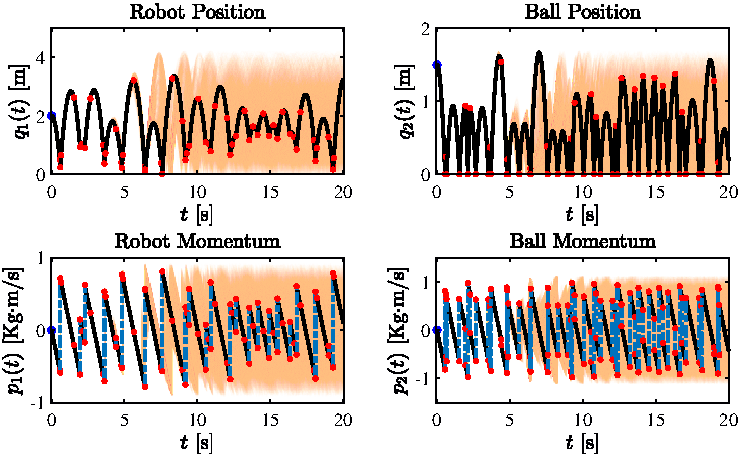
\includegraphics[width = \linewidth]{Figures/chaos1.pdf}
%    \caption[Time evolution of the autonomous system' state in the Monte Carlo simulation]{Time evolution of the autonomous system' state in the Monte Carlo simulation. The black trajectory is the nominal one (starting from $\xb_0$), where red dots and dashed blue lines indicate discrete events (impacts) and the value of the state after the events, respectively. Orange lines show the traces of all the other trajectories of the Monte Carlo runs (with initial condition sampled from $\N(\xb_0,\sigma\mathbb{I}_n)$). The blue dots at $t=0$ are the initial conditions. It can be noticed how trajectories, starting very close, diverge, densely covering the state--space.}
%    \label{fig:chaos1}
%\end{figure}
%%
%
%This phenomenon is further emphasized by looking at the phase--space trajectories of the robot and the ball, respectively, represented in Fig. \ref{fig:chaos2}. 
%%
%\begin{figure}[!ht]
%    \centering
%    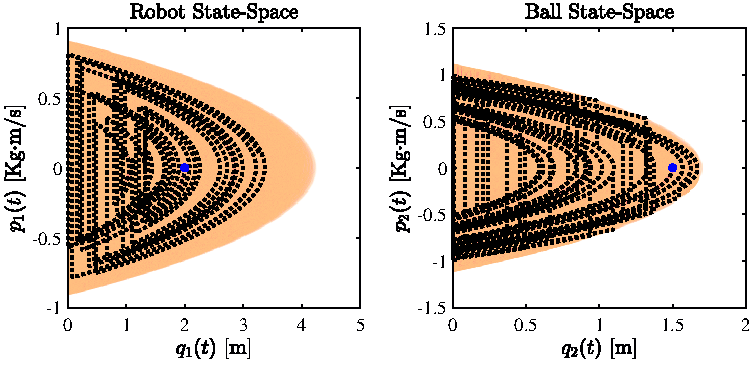
\includegraphics[width = \linewidth]{Figures/chaos2.pdf}
%    \caption[Phase--space trajectory of the autonomous system in the Monte Carlo simulation]{Phase--space trajectory of the autonomous system in the Monte Carlo simulation. The dashed black line is the nominal one (starting from $\xb_0$). Orange lines show the traces of all the other trajectories of the Monte Carlo runs (with initial condition sampled from $\N(\xb_0,\sigma\mathbb{I}_n)$). The blue dots at are the initial conditions. It can be noticed how trajectories, starting very close, diverge, densely covering the state--space.}
%    \label{fig:chaos2}
%\end{figure}
%%
%\begin{figure}[!ht]
%    \centering
%    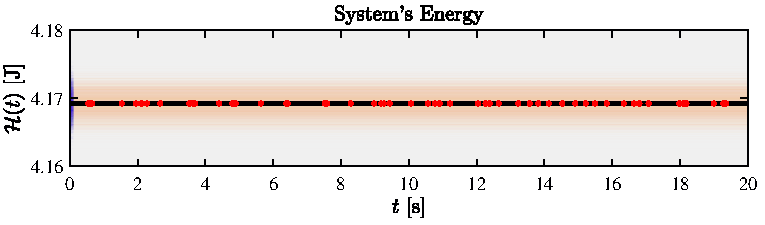
\includegraphics[width = \linewidth]{Figures/chaos3.pdf}
%    \caption[Time evolution of the energy in the Monte Carlo simulation]{Time evolution of the energy in the Monte Carlo simulation. The black trajectory is the nominal one (starting from $\xb_0$), where red dots indicate discrete events (impacts). Orange lines show the traces of all the other trajectories of the Monte Carlo runs (with initial condition sampled from $\N(\xb_0,\sigma\mathbb{I}_n)$). The blue dots at $t=0$ are the initial energies of each Monte Carlo run. It can be noticed how, regardless the initial condition, energy is conserved in time.}
%    \label{fig:chaos3}
%\end{figure}
%
%The time evolution of the energy (Hamiltonian function) among the Monte Carlo runs is also shown in Fig. \ref{fig:chaos3}. As expected, the energy is conserved trough time.
%%
%
%%
%The experiment which has been done here numerically can be formalized as follows.
%Instead of an initial condition $\x_0$, an initial (probability) density of the state in space
%%
%\begin{equation}
%	\psi(\xb_0)=\N(\xb_0,\sigma\mathbb{I}_n)
%\end{equation}
%%
%has been considered and we observed how this distribution evolved in time through the dynamics of the system, i.e. the solution of a distributed parameters system has been numerically approximated.
%%partial differential equation of type
%%%
%%\begin{equation}
%%    \partial_t\psi(\xb) = \Gamma(\psi(\xb)).
%%\end{equation}
%%%
%%
%
%\clearpage
%From the numerical experiment's results, the histograms of state density in space at each time instant have been built. 
%The initial and final spatial density functions
%%
%\begin{equation}
%	\psi_i\triangleq\psi(\x_0)= \N(\xb_0,\sigma\mathbb{I}_n),~~ \psi_f = \psi(\xb(t = 20s))
%\end{equation}
%%
%displayed in Fig. \ref{fig:hist}.
%%
%\begin{figure}[!ht]
%	\centering
%	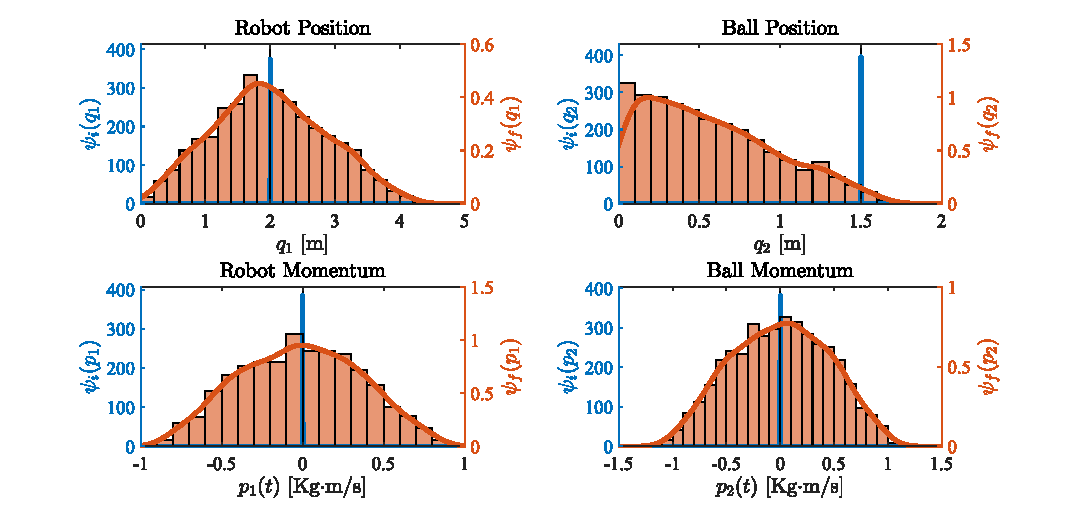
\includegraphics[width = 1\linewidth]{Figures/Hist.pdf}
%	\caption[Histograms and reconstructed spatial (probability) density functions of the state]{Histograms and reconstructed spatial (probability) density functions of the state. Blue and orange histograms (lines) represent, respectively, initial and final spatial densities of each state.}
%	\label{fig:hist}
%\end{figure}
%%
%
%Then, the time evolution of state probability distribution \footnote{i.e., the probability of finding the state of the system somewhere in the state--space.} have been plot (in a phasegram) for each state of the system. Results are reported in Figure \ref{fig:phasegram}. 
%%
%\begin{figure}[!ht]
%    \centering
%    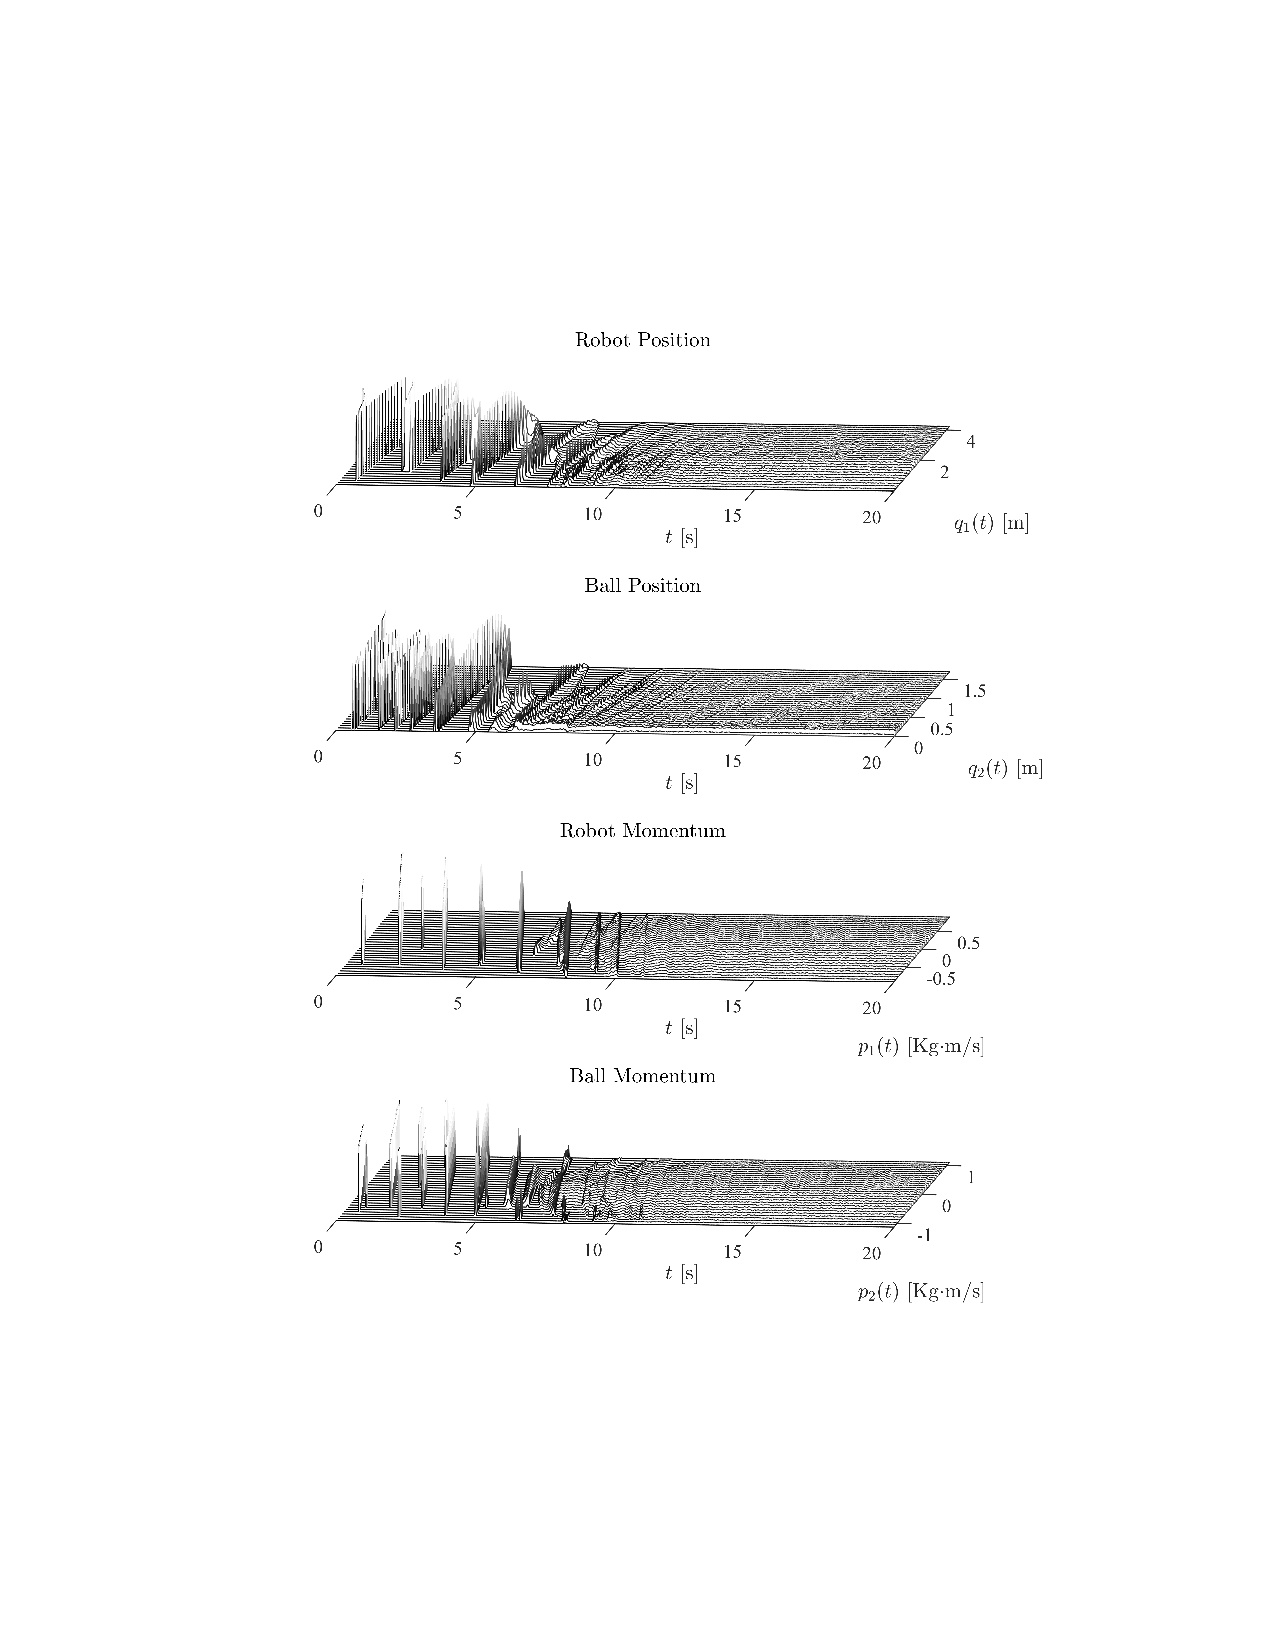
\includegraphics[width = 1\linewidth, trim={5cm 5.75cm 3.9cm 5.5cm},clip]{Figures/PhaseGram.pdf}
%    \caption[Phasegram of the state spatial density function]{Phasegram of the state spatial (probability) density function computed from the Monte Carlo experiment. At $t=0$ the state spatial density is just a spike across the initial condition. Throughout time, the density relaxes to a much larger variance function.}
%    \label{fig:phasegram}
%\end{figure}
%%
%
%At $t=0$ the state probability is just a \textit{spike} across the nominal initial condition. Throughout time, however, the spatial (probability) of each state relaxes to a function with much larger variance.
%The outcome of this experiment is the following: although all trajectories started very close one to the other, after a short period of time, the state could be almost everywhere in the state--space. Thus, the essence of the autonomous conservative ball--dribbling robot, resembles the one of a stochastic process although it is deterministic in nature.
Let us consider the uncontrolled system and set the physical parameters so that the system is conservative, i.e. $c_i = c_g = 1$, $\beta_1=\beta_2=0$. In this case, the Hamiltonian is constant,
%
\begin{align}
%
&\forall t\geq 0,\xb\in\C &&\dot{\Ha}(\xb(t)) = 0,\\
%
&\forall t\geq 0,\xb\in\D,\gb\in\G && \Ha(\gb(\xb(t)))-\Ha(\xb(t))=0.
%
\end{align}
%

Thus, trajectories lie on foliations of level sets Hamiltonian corresponding to possible initial conditions $\xb_0$:
%
\begin{equation}
\forall t\geq 0 \quad \xb(t)\in\left\{\xb:\Ha(\xb) = \Ha(\x_0)\right\}
\end{equation}
%
and the Liouville theorem (a reference is necessary HERE) (in the form of Boltzmann equation) also guarantees conservation of the phase--space measure.
%

However, although the system is linear, chaos emerges due to the presence of impacts. The system is in fact characterized by an exceptional sensitivity to the initial condition: trajectories starting ``very close'' tend to diverge in time (within the limited phase--space).
%

With the aim of revealing the dawn of chaos, a numerical experiment has been performed in the modus operandi of a Monte Carlo simulation. The system has been integrated for 3000 different initial conditions $\xb_0^i$ sampled by a multivariate normal distribution centered in a nominal initial condition $\xb_0$ and with variance $\sigma = 10^{-6}$:
%
\begin{equation}
\xb_0^i \sim \N(\xb_0,\sigma\mathbb{I}_n).
\end{equation}
%
\begin{figure}[t!]
	\centering
	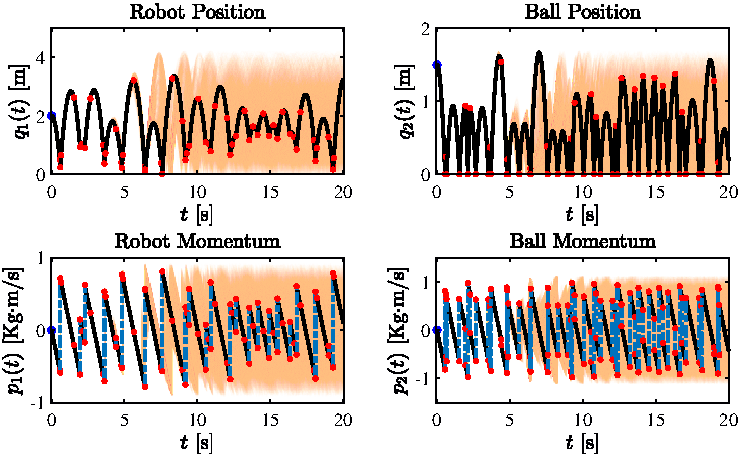
\includegraphics[width = \linewidth]{Figures/chaos1.pdf}
	\caption[Time evolution of the autonomous system' state in the Monte Carlo simulation]{Time evolution of the autonomous system' state in the Monte Carlo simulation. The black trajectory is the nominal one (starting from $\xb_0$), where red dots and dashed blue lines indicate discrete events (impacts) and the value of the state after the events, respectively. Orange lines show the traces of all the other trajectories of the Monte Carlo runs (with initial condition sampled from $\N(\xb_0,\sigma\mathbb{I}_n)$). The blue dots at $t=0$ are the initial conditions. It can be noticed how trajectories, starting very close, diverge, densely covering the state--space.}
	\label{fig:chaos1}
\end{figure}
Choosing $\x_0\triangleq(2,1.5,0,0)$, $m_1 = 1\text{Kg}$ and $m_2 = 0.15\text{Kg}$, the nominal trajectory and the other 3000 ones have been integrated for $t = 20s$. The experiments have been carried out with the \textit{Hybrid Equations (HyEQ) Toolbox} \citep{sanfelice2013toolbox} for the \textsc{Matlab} environment. The time evolution of the system's state in all the trials is shown in Fig. \ref{fig:chaos1}. The black trajectory represents the nominal one (starting from $\xb_0$), where red dots and dashed blue lines indicate discrete events (impacts) and the value of the state after the events, respectively. Orange lines show the traces of all other trajectories for each Monte Carlo run. The blue dots at $t=0$ are the initial conditions. It can be noticed how trajectories, starting indistinguishably close, diverge, densely covering to the state--space.
%

%

This phenomenon is further emphasized in Fig. \ref{fig:chaos2}, which shows the phase--space trajectories of the robot and the ball, respectively. 
%
\begin{figure}[!ht]
	\centering
	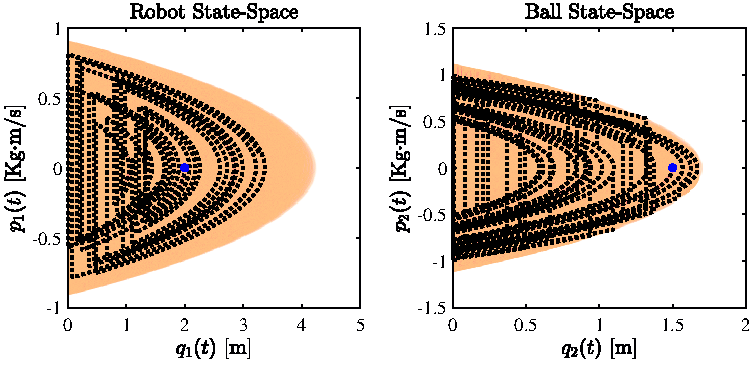
\includegraphics[width = \linewidth]{Figures/chaos2.pdf}
	\caption[Phase--space trajectory of the autonomous system in the Monte Carlo simulation]{Phase--space trajectory of the autonomous system in the Monte Carlo simulation. The dashed black line is the nominal one (starting from $\xb_0$). Orange lines show the traces of all the other trajectories of the Monte Carlo runs (with initial condition sampled from $\N(\xb_0,\sigma\mathbb{I}_n)$). The blue dots at are the initial conditions. It can be noticed how trajectories, starting very close, diverge, densely covering the state--space.}
	\label{fig:chaos2}
\end{figure}
%
\begin{figure}[hb!]
	\centering
	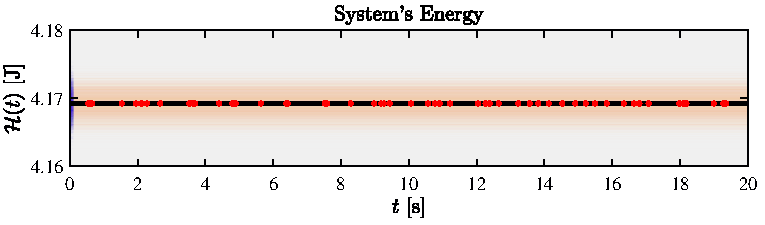
\includegraphics[width = \linewidth]{Figures/chaos3.pdf}
	\caption[Time evolution of the energy in the Monte Carlo simulation]{Time evolution of the energy in the Monte Carlo simulation. The black trajectory is the nominal one (starting from $\xb_0$), where red dots indicate discrete events (impacts). Orange lines show the traces of all the other trajectories of the Monte Carlo runs (with initial condition sampled from $\N(\xb_0,\sigma\mathbb{I}_n)$). The blue dots at $t=0$ are the initial energies of each Monte Carlo run. It can be noticed how, regardless the initial condition, energy is conserved in time.}
	\label{fig:chaos3}
\end{figure}

The time evolution of the energy (Hamiltonian function) among the Monte Carlo runs is also shown in Fig. \ref{fig:chaos3}. As expected, the energy is conserved trough time.
%

%
The experiment which has been done here numerically can be formalized as follows.
Instead of an initial condition $\x_0$, an initial (probability) density of the state in space
%
\begin{equation}
\psi(\xb_0)=\N(\xb_0,\sigma\mathbb{I}_n)
\end{equation}
%
has been considered and the evolution in time of this distribution has been observed through the dynamics of the system, i.e. the solution of a distributed parameters system has been numerically approximated.
%partial differential equation of type
%%
%\begin{equation}
%    \partial_t\psi(\xb) = \Gamma(\psi(\xb)).
%\end{equation}
%%
%

From the numerical experiment's results, the histograms of state density in space at each time instant have been built. 
The initial and final spatial density functions
%
\begin{equation}
\psi_i\triangleq\psi(\x_0)= \N(\xb_0,\sigma\mathbb{I}_n),~~ \psi_f = \psi(\xb(t = 20s))
\end{equation}
%
displayed in Fig. \ref{fig:hist}.

The time evolution of state probability distribution \footnote{i.e. the probability of finding the state of the system somewhere in the state--space.} have been plotted (in a phase-gram) for each state of the system. Results are reported in Figure \ref{fig:phasegram}. 

\begin{figure}[t!]
	\centering
	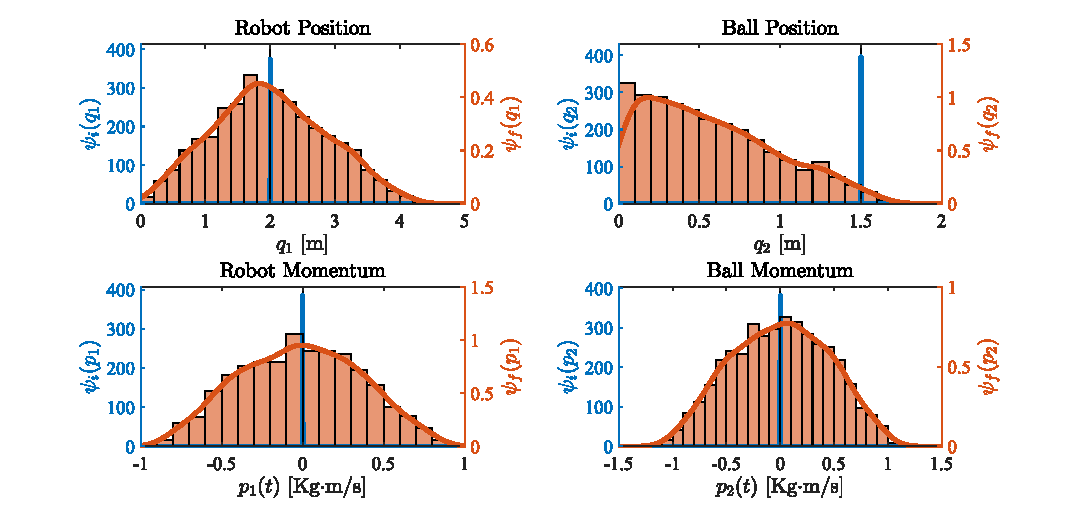
\includegraphics[width = 1\linewidth]{Figures/Hist.pdf}
	\caption[Histograms and reconstructed spatial (probability) density functions of the state]{Histograms and reconstructed spatial (probability) density functions of the state. Blue and orange histograms (lines) represent, respectively, initial and final spatial densities of each state.}
	\label{fig:hist}
\end{figure}

\begin{figure}[!ht]
	\centering
	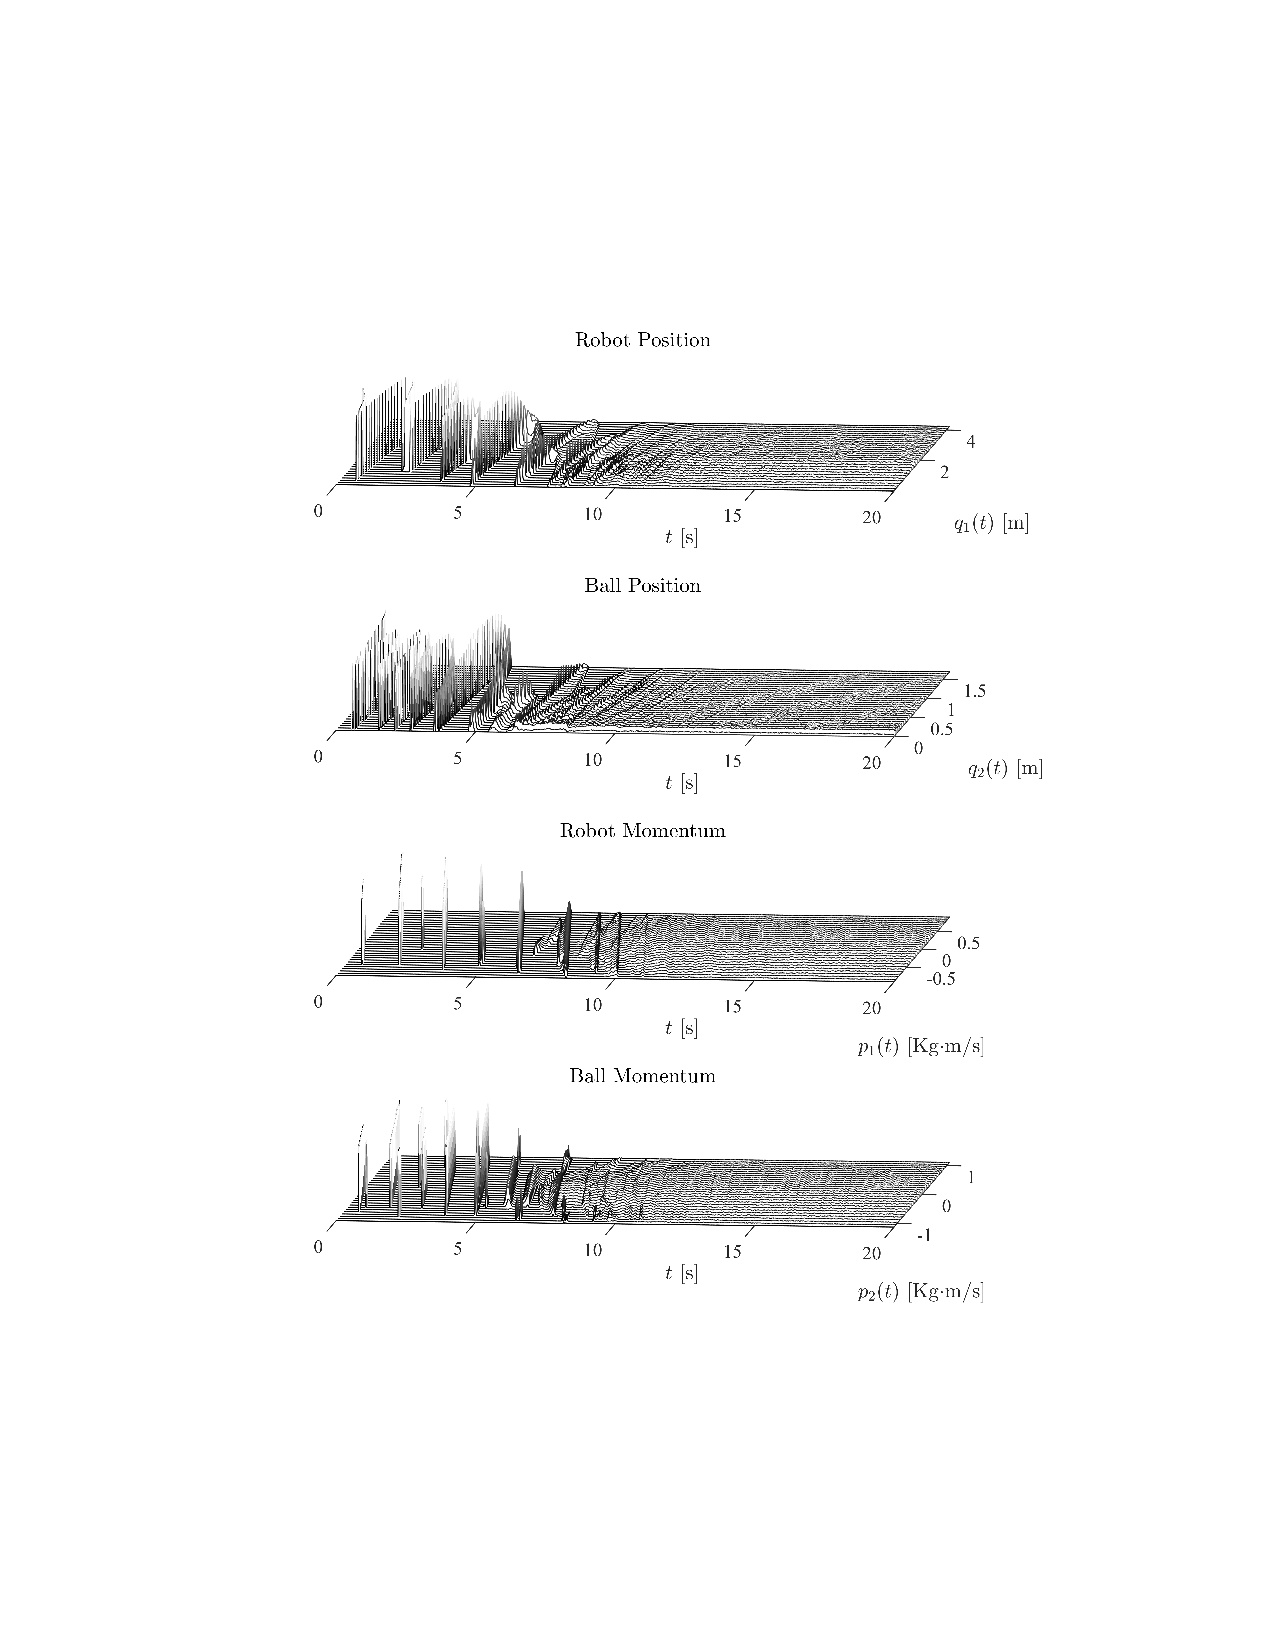
\includegraphics[width = 1\linewidth, trim={5cm 5.75cm 3.9cm 5.5cm},clip]{Figures/PhaseGram.pdf}
	\caption[Phase--gram of the state spatial density function]{Phase--gram of the state spatial (probability) density function computed from the Monte Carlo experiment. At $t=0$ the state spatial density is just a spike across the initial condition. Throughout time, the density relaxes to a function with larger variance.}
	\label{fig:phasegram}
\end{figure}
%

At $t=0$ the state probability is just a \textit{spike} across the nominal initial condition. Throughout time, however, the spatial (probability) of each state relaxes to a function with much larger variance.
This experiment demonstrated that, although all trajectories started very close one to each other, after a short period of time, the state can be almost everywhere in the state--space. Thus, the essence of the autonomous conservative ball--dribbling robot, resembles the one of a stochastic process, despite the fact that  it is deterministic in nature.
\clearpage
%%%%%%%%%%%%%%%%%%%%%%%%%%%%%%%%%%%%%%%%%%%%%%%%%%%%%%%%%%%%%%%%%%%%%%%%
\section{Dribbling Control}\label{sec:control}
%
Let us consider the control task of continuously hitting the ball such that it reaches, at every cycle, the same maximum height $q_{2,max}^*$. In order to address this control problem, it is possible to design an hybrid controller with two modes, i.e., a \textit{wait mode} ($S_{w}$) and a \textit{hit mode} ($S_{h}$). In the wait state, the robot must stay at a constant height above the ball, to overcome any interference between its motion and the one of the ball and, at the same time, stay close enough to the ball to hit it quickly at the right time.
Then, in the hit state, the controller must move the robot toward the ball so that the exchanged impulse during the impact would lead the ball to come back to the desired peak $q_{2,max}^*$. In particular, the system would enter in the hit state whenever the ball reaches the peak of its bounce and switch back to the wait mode immediately after the impact between the two bodies. 
%
In both modes, it is desirable to exploit the passivity--based control theory. Besides, the system is under--actuated and the flows are decoupled. Therefore, it is impossible to shape the total energy of system setting its minimum in a desired configuration different from the origin. Although it is not possible to modify the energy of the ball, it is however possible to partially shape the Hamiltonian, i.e. the part relative to the robot. If 
%
\begin{equation}
    \Ha(\xb) = \Ha_1(q_1,p_1) + \Ha_2(q_2,p_2),
\end{equation}
%
it is possible to obtained a desired-shape Hamiltonian
%
\begin{equation}
     \Ha^*(\xb)  = \Ha_1^*(q_1,p_1) + \Ha_2(q_2,p_2),
\end{equation}
%
allowing to bring the robot in a desired configuration $q_1^*$. This might be achieved through an \textit{energy--balancing passivity--based controller}\footnote{In this case $q_1^*$ becomes a strict minimum of $\Ha_1^*$ and asymptotic stabilization must be achieved with $p_1 = 0$ at steady--state} \citep{ortega2001putting,ortega2008control,secchi2007control} described in Chapter \ref{chap:preliminaries}:
%
\begin{align}
u &= \beta(\xb) + v = \beta(\xb) - k_dy \\
&= \frac{\partial V_1(q_1)}{\partial q_1} - k_p(q_1 -q_1^*) - k_d\dot{q}_1\\
&= \gamma m_1q_1- k_p(q_1 -q_1^*) - k_d\dot{q}_1.
\end{align}
%

As pointed out before, the controller has two separate modes and the control parameters $k_p$, $k_d$, $q_1^*$ should be changed during the state transitions.
% 
For this reason, let us collect the control parameters in a vector 
%
\begin{equation}
    \bm\omega = (k_p,k_d,q_1^*)
\end{equation}
%
and consider it as part of the state vector. The augmented model of the controlled system can be then rewritten as follows:
\begin{equation}\label{eq:HpHc}
    %
    \left\{ 
        \begin{matrix*}[l]\vspace{1pt}
            %
            \begin{bmatrix}\dot{\xb}\\\dot{\bm\omega}\end{bmatrix} = \begin{bmatrix}\left[\Jb-\Rb\right]{\dH^*(\xb)}+\Gb v(\x,\bm\omega)\\\mymathbb{0}_3\end{bmatrix} &(\xb,\bm\omega,v)\in\C\times\Omega\times\U\\
            %
            \begin{bmatrix}{\xb}^+\\{\bm\omega}^+\end{bmatrix} \in \G\times\Lambda&(\xb,\bm\omega)\in\D\times\Omega\\
            %
            y = \Gb^\top{\dH^*(\xb)}
        \end{matrix*}
    \right.~~,
    %
\end{equation}
%
where $\Omega$ is the space of admissible parameters values and $\Lambda$ is the jump set--valued mapping of the control parameters. The shaped Hamiltonian $\Ha^*(\xb,\bm\omega)$, results to be
%
\begin{equation}
	\Ha^*(\xb,\bm\omega) = \frac{1}{2}\pb^\top \Mb^{-1}\pb + \frac{1}{2}k_p(q_1 - q_1^*)^2+ \gamma m_2q_2.
\end{equation}
%

Notice that the choice of the control parameters influences both the closed-loop energy $\Ha^*$ (with $k_p$ and $q_1^*$) and the output feedback $v$ (with $k_d$).
%
Let us define a jump set $\D_3$ corresponding to the sub--manifold of the state--space where the ball reaches the peak $q_{2,max}$ of its bounce: $\D_3 = \left\{\xb:~p_2=0\right\}$.
It is clear that during the time evolution of the system, the state will cyclically enter in $\D_3$ and therefore the controller will periodically switch to $S_h$ where the robot moves toward the ball until they collide, i.e. $\xb\in\D_2$, when the controller switches back to $S_w$ where the robot waits above the ball at a distance $\delta$. The jumps maps resetting the control parameters are the following:
%
\begin{align}
\bm\omega^+ = \bm\nu_{3}(\xb,\bm\omega) &=\begin{bmatrix}k_{p,h}&k_{d,h}&q_2\end{bmatrix}^\top &\quad&\xb\in\D_3,\\
\bm\omega^+ = \bm\nu_{2}(\xb,\bm\omega) &=\begin{bmatrix}k_{p,w}&k_{d,w}&q_2 + \delta\end{bmatrix}^\top &\quad&\xb\in\D_2,\\
\bm\omega^+ = \bm\nu_{1}(\xb,\bm\omega) &= \bm\omega &\quad&\xb\in\D_1.
\end{align}
%

Therefore,
%
\begin{equation}
    \Lambda \triangleq \left\{{\bm\nu}_i:\xb\in\D_i\Rightarrow \bm\omega^+ = \bm\nu_i(\bm\omega,\xb),~ i = 1,2,3\right\}.
\end{equation}
%

Figure \ref{fig:ctrl} shows the finite--state machine representing the controller.
When $\xb\in\D_3$, the state of the system does not jump, i.e. $\xb^+ = \gb_3(\xb)= \xb$ if $\xb\in\D_3$.
The set-valued mapping $\G$ is redefined considering $\gb_3$.
%
\begin{figure}[!ht]
	\centering
	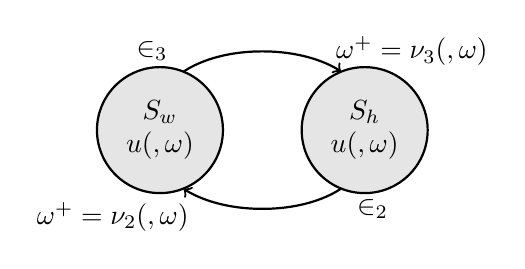
\begin{tikzpicture}
	%
	\fill[gray!20, draw = black,thick] (-1.3,0) circle (0.8cm);
	\fill[gray!20, draw = black,thick] (1.3,0) circle (0.8cm);
	%	
	\draw (-1.3,0) node[align = center](flow)  {$S_{w}$\\$u(\xb,\bm\omega)$};
	\draw (1.3,0) node[align = center](flow)  {$S_{h}$\\$u(\xb,\bm\omega)$};
	%
	\draw [thick,->] plot [smooth, tension=1.2] coordinates { (-1,0.74162) (0,1) (1,0.74162)};
	\draw [thick,->] plot [smooth, tension=1.2] coordinates { (1,-0.74162) (0,-1) (-1,-0.74162)};
	%
	\draw (1.9,1) node {$\bm\omega^+ = \bm\nu_{3}(\xb,\bm\omega)$};
	\draw (1.4,-1) node {$\xb\in\D_2$};
	%
	%
	\draw (-1.9,-1.1) node {$\bm\omega^+ = \bm\nu_{2}(\xb,\bm\omega)$};
	\draw (-1.4,1) node {$\xb\in\D_3$};
	%
	\end{tikzpicture}
	\caption[Finite state machine of the controller]{Finite state machine of the controller. It has an \textit{hit} state $S_h$ in which it forces the robot to move toward the ball and a \textit{wait} state $S_w$ in which it keeps the robot at a constant distance $\delta$ from the ball.The transitions happen as follows: $S_h\rightarrow S_w$ when the robot hits the ball, $S_w\rightarrow S_h$ when the ball reaches the peak of its bounce.}
	\label{fig:ctrl}
\end{figure}
%
\begin{rem}
    The behavior of the system strongly depends on the choice of the control parameters. Furthermore, unless a solution of (\ref{eq:HpHc}) is derived, it is not possible to find analytically two sets of control parameters (one for $S_{w}$ and one for $S_{h}$) which solve the control problem, i.e. ensuring that the ball bounces continuously reaching each time the desired peak $q_{2,max}^*$.
\end{rem}
 For the reasons stated in previous remark, a new paradigm of energy based control, which combines the traditional energy shaping approach with a basic form of {iterative learning control}: the \textit{iterative energy shaping}, has been introduced.
\begin{defn}[Iterative Energy Shaping Control]$\newline$
	First, let us define some further control parameters which are needed for the design.
	Let $\xi$ be a counter of the number of cycles of the system, i.e., the number of complete bounces of the ball. Let initialize $\xi$ to one. Let $e(\xi) = q_{2,max}^* - q_{2,max}$ computed when $\xb\in\D_3$ be the tracking error of the iterative energy shaping control loop. Thus, the control parameters vector can be redefined as 
	%
	\begin{equation}
	    \bm\omega \triangleq (k_p,k_d,q_1^*,\xi).
	\end{equation}
	%
	
	The iterative energy shaping control law is defined by means of the following control parameters jump maps:
	%
	\begin{align}
	&\bm\omega^+  \triangleq \bm\nu_{3}(\xb,\bm\omega)=\begin{bmatrix}k_0\varphi_\xi(e)&k_{d,h}&q_2&\xi+1\end{bmatrix}^\top &\xb\in\D_3,\\
	&\bm\omega^+  \triangleq \bm\nu_{2}(\xb,\bm\omega)=\begin{bmatrix}k_{p,w}&k_{d,w}&q_2 + \delta&\xi\end{bmatrix}^\top &\xb\in\D_2,
	\end{align}
	%
	where $\sigma>0$ is a constant scalar and $\varphi_\xi(e)$ is a scalar function of the error. When the controller is in the \textit{hit} state, the resulting shaped Hamiltonian assumes the following form:
	\begin{equation}
		\Ha^*(\xb,\bm\omega) = \frac{1}{2}\pb^\top \Mb^{-1}\pb + \frac{1}{2}k_0\varphi_\xi(e)(q_1 - q_1^*)^2+ \gamma m_2q_2.
	\end{equation}
\end{defn}
%
A representation of the \textit{hybrid automata} corresponding to the final controlled system is pictured in Fig. \ref{fig:cHPH}.
%
\begin{figure}[!ht]
	%
	\centering
	%
	\scalebox{1}{
		\begin{tikzpicture}
		% 
		\fill[gray!20, draw = black,thick] (0,0) ellipse (2.5cm and 1.5cm);
		%	
		\draw (0,0) node[align = center](flow)  {$\xb\in\C$\\\\$\begin{bmatrix}\dot{\xb}\\\dot{\bm\omega}\end{bmatrix} = \begin{bmatrix}\left[\Jb-\Rb\right]\dH^*(\xb)+\Gb v\\\mymathbb{0}_4\end{bmatrix}$\\$y = \Gb^\top\dH^*(\xb)$};
		%
		\draw [thick,->] plot [smooth, tension=2] coordinates { (-0.5,1.4697) (0,2.2) (0.5,1.4697)};
		\draw [thick,->] plot [smooth, tension=2] coordinates { (2.5,0) (2.9,-.7) (2.1,-0.8139)};
		\draw [thick,->] plot [smooth, tension=2] coordinates { (-2.5,0) (-2.9,-.7) (-2.1,-0.8139)};
		%
		\draw (3.1,0.2) node {$\xb\in\D_2$};
		\draw (2.9,-1.75) node[align = left] {$\begin{bmatrix}\xb^+\\\bm\omega^+\end{bmatrix} = \begin{bmatrix}\gb_2(\xb)\\\bm\nu_2(\xb,\bm\omega)\end{bmatrix}$};
		%
		\draw (-3.1,0.2) node {$\xb\in\D_1$};
		\draw (-2.7,-1.75) node[align = left] {$\begin{bmatrix}\xb^+\\\bm\omega^+\end{bmatrix} = \begin{bmatrix}\gb_1(\xb)\\\bm\nu_1(\xb,\bm\omega)\end{bmatrix}$};;
		%
		\draw (-1.1,1.7) node {$\xb\in\D_3$};
		\draw (2.2,1.9) node[align = left] {$\begin{bmatrix}\xb^+\\\bm\omega^+\end{bmatrix} = \begin{bmatrix}\gb_3(\xb)\\
		\bm\nu_3(\xb,\bm\omega)\end{bmatrix}$};
		%
		\end{tikzpicture}
	}
	\caption[Hybrid automata representing the controlled system]{Hybrid automata representing the controlled system. Although the \textit{iterative energy shaping} controller has two modes, the controlled system is still an impulsive port--Hamiltonian system}
	\label{fig:cHPH}
\end{figure}
%
The main idea is to iteratively adjust the slope (steepness) of the energy of the system as function of the error. For instance, when $e>0$, it can be derived that the robot had hit the ball with not enough momentum. Thus, at the next cycle, the energy function should be steeper so that the robot will accelerate faster toward the ball, since the dissipation rate $k_d$ of the damping injection didn't change. The same concept can be adopted for $e<0$, by making the the energy function less steep.
%
A possible choice of $\varphi_\xi(e)$ is
%
\begin{equation}
    \varphi_\xi(e)  \triangleq \varphi_0 + a\cdot e(\xi) + b\cdot\sum_{i = 1}^{\xi}e(i),
\end{equation}
%
which provides a proportional and integral action with a constant offset $\varphi_0$ in response to the error. The integral action should ensure zero steady state error.
%
\section{Numerical Simulations}
%
To validate the proposed control scheme, numerical simulations have been performed. The physical parameters of the system have been chosen as $m_1 = 0.1\text{Kg}$, $m_2 = 0.05\text{Kg}$, $\beta_1 = 0.2\text{N}\cdot \text{s}/\text{m}$, $\beta_2 = 0.3\text{N}\cdot \text{s}/\text{m}$, $c_g = c_i = 0.8$. The initial conditions have been set to $q_1(0) = 2$m, $q_2(0) = 1.5$m, $p_1(0) = p_2(0) = 0\text{Kg}\cdot \text{m}/\text{s}$. Note that the mass of the ball $m_2$ has been chosen similar to the one of a standard golf ball ($\approx 46g$).
%%%%%%%%%%%%%%%%%%%%%%%%%%%%%
%\subsection{Autonomous System}
%%
%Firstly, the behavior of the uncontrolled system has been simulated. The time evolution of the state variables are shown in Fig. \ref{fig:aut1}.
%%
%\begin{figure}[!ht]
%	\centering
%	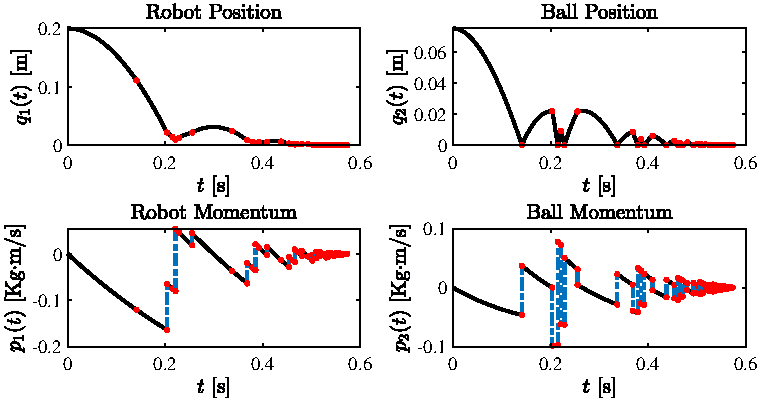
\includegraphics[width = \linewidth]{Figures/aut1.pdf}
%	\caption[Uncontrolled system: time evolution of the robot and ball position states]{Uncontrolled system: time evolution of the robot and ball position states (position and momentum). Red dots correspond to system's jumps while dashed blue lines highlight discontinuous state changes. Notice that both the position and velocity goes asymptotically to zero.}
%	\label{fig:aut1}
%\end{figure}
%%
%The phase--space trajectory of the autonomous system is also represented in Fig. \ref{fig:aut2} over the energy of the system. 
%%
%\begin{figure}[!ht]
%	\centering
%    \definecolor{ocean}{rgb}{0.00000,0.44700,0.74100}
\definecolor{mycolor1}{rgb}{0.00000,0.44700,0.74100}%

\begin{tikzpicture}
\begin{axis}[
width=5cm,
height=5cm,
at={(1in,0.331in)},
view={0}{90},
colorbar horizontal,
colormap = {whiteblack}{color(0cm)  = (white);color(1cm) = (black)},
colorbar style = {at = {(0,-0.25)}},
xmin=0,
xmax=.2,
xlabel style={font=\color{white!15!black},at = {(0.75in,-0.125in)}},
xlabel={$q_1(t)~[m]$},
ymin=-.2,
ymax=.1,
ylabel style={font=\color{white!15!black},at = {(-0.1in,0.75in)}},
ylabel={$p_1(t)~$[Kg$\cdot$m/s]},
title = {robot phase--space},
axis background/.style={fill=white},
]
\addplot3[contour filled={number = 25,labels={false}},mesh/rows=25,mesh/cols=25,mesh/check=false,forget plot
] table {H1_a.dat};
%%%%%%%%%%%%%%%%%%%%%%%%%%%%%%%%%%%%
\addplot [color=black, line width=1.5pt]
  table[row sep=crcr]{%
0.2	0\\
0.2	0\\
0.199999967381998	-7.99934763995355e-05\\
0.199998826071083	-0.000479765214216573\\
0.199989131483394	-0.00145882629667888\\
0.199969656068965	-0.00243593121379302\\
0.1999404193699	-0.00341108387397995\\
0.199901440889258	-0.00438428817785163\\
0.199852740091133	-0.00535554801822656\\
0.199794336400727	-0.00632486728014541\\
0.199726249204433	-0.00729224984088653\\
0.199648497849907	-0.00825769956998144\\
0.199561101646152	-0.00922122032923035\\
0.199464079863588	-0.0101828159727176\\
0.199357451734135	-0.011142490346827\\
0.199241236451287	-0.0121002472902574\\
0.199115453170189	-0.0130560906340378\\
0.198980121007714	-0.0140100242015429\\
0.198835259042541	-0.0149620518085082\\
0.198680886315227	-0.0159121772630453\\
0.198517021828288	-0.0168604043656575\\
0.198343684546272	-0.0178067369092544\\
0.198160893395837	-0.0187511786791674\\
0.197968667265824	-0.0196937334531649\\
0.197767025007336	-0.0206344050014671\\
0.197555985433808	-0.0215731970867617\\
0.19733556732109	-0.0225101134642181\\
0.197105789407515	-0.0234451578815031\\
0.196866670393978	-0.0243783340787956\\
0.196618228944009	-0.0253096457888017\\
0.196360483683848	-0.0262390967367695\\
0.19609345320252	-0.027166690640504\\
0.19581715605191	-0.028092431210382\\
0.195531610746835	-0.0290163221493671\\
0.195236835765121	-0.0299383671530242\\
0.194932849547673	-0.0308585699095347\\
0.194619670498553	-0.0317769340997106\\
0.194297316985051	-0.0326934633970102\\
0.193965807337758	-0.0336081614675517\\
0.193625159850643	-0.0345210319701286\\
0.193275392781121	-0.0354320785562243\\
0.192916524350131	-0.0363413048700261\\
0.192548572742204	-0.0372487145484408\\
0.19217155610554	-0.038154311221108\\
0.191785492552079	-0.0390580985104158\\
0.191390400157573	-0.0399600800315146\\
0.190986296961657	-0.0408602593923315\\
0.190573200967926	-0.0417586401935853\\
0.190151130144001	-0.0426552260288003\\
0.189720102421606	-0.0435500204843211\\
0.189280135696634	-0.0444430271393267\\
0.188831247829225	-0.045334249565845\\
0.188373456643834	-0.0462236913287668\\
0.187906779929302	-0.0471113559858603\\
0.187431235438927	-0.0479972470877854\\
0.186946840890538	-0.0488813681781077\\
0.186453613966563	-0.0497637227933127\\
0.1859515723141	-0.05064431446282\\
0.185440733544988	-0.0515231467089975\\
0.184921115235877	-0.0524002230471754\\
0.184392734928301	-0.0532755469856602\\
0.183855610128744	-0.0541491220257488\\
0.183309758308713	-0.0550209516617425\\
0.182755196904805	-0.0558910393809611\\
0.182191943318783	-0.0567593886637566\\
0.181620014917636	-0.0576260029835272\\
0.181039429033657	-0.0584908858067314\\
0.180450202964509	-0.0593540405929017\\
0.179852353973292	-0.0602154707946584\\
0.179245899288617	-0.0610751798577234\\
0.17863085610467	-0.0619331712209341\\
0.178007241581285	-0.0627894483162571\\
0.17737507284401	-0.0636440145688019\\
0.176734366984174	-0.0644968733968348\\
0.17608514105896	-0.0653480282117921\\
0.175427412091471	-0.0661974824182942\\
0.174761197070796	-0.0670452394141591\\
0.17408651295208	-0.067891302590416\\
0.173403376656593	-0.0687356753313186\\
0.172711805071795	-0.0695783610143591\\
0.172011815051406	-0.0704193630102812\\
0.171303423415471	-0.0712586846830942\\
0.170586646950429	-0.0720963293900858\\
0.16986150240918	-0.072932300481836\\
0.169128006511151	-0.0737666013022302\\
0.168386175942364	-0.0745992351884729\\
0.167636027355503	-0.0754302054711006\\
0.166877577369979	-0.0762595154739958\\
0.166110842571997	-0.0770871685143994\\
0.165335839514624	-0.0779131679029247\\
0.164552584717852	-0.0787375169435705\\
0.163761094668669	-0.0795602189337339\\
0.16296138582112	-0.080381277164224\\
0.162153474596374	-0.0812006949192748\\
0.161337377382792	-0.0820184754765585\\
0.160513110535992	-0.0828346221071984\\
0.15968069037891	-0.083649138075782\\
0.158840133201872	-0.0844620266403744\\
0.157991455262655	-0.0852732910525309\\
0.157134672786551	-0.0860829345573103\\
0.156269801966437	-0.0868909603932875\\
0.155396858962835	-0.0876973717925671\\
0.154515859903979	-0.0885021719807957\\
0.153626820885876	-0.0893053641771752\\
0.152729757972377	-0.0901069515944754\\
0.151824687195235	-0.090906937439047\\
0.150911624554173	-0.0917053249108346\\
0.149990586016945	-0.092502117203389\\
0.149061587519402	-0.0932973175038804\\
0.148124644965556	-0.0940909289931113\\
0.147179774227642	-0.0948829548455284\\
0.146226991146182	-0.0956733982292365\\
0.145266311530049	-0.0964622623060099\\
0.144297751156531	-0.0972495502313062\\
0.14332132577139	-0.0980352651542779\\
0.14233705108893	-0.098819410217786\\
0.141344942792058	-0.0996019885584117\\
0.140345016532346	-0.100383003306469\\
0.139337287930095	-0.101162457586019\\
0.138321772574394	-0.101940354514879\\
0.137298486023188	-0.102716697204638\\
0.136267443803336	-0.103491488760667\\
0.135228661410673	-0.104264732282135\\
0.134182154310077	-0.105036430862015\\
0.133127937935522	-0.105806587587104\\
0.13206602769015	-0.10657520553803\\
0.130996438946323	-0.107342287789265\\
0.129919187045693	-0.108107837409139\\
0.128834287299257	-0.108871857459852\\
0.127741754987421	-0.109634350997484\\
0.12664160536006	-0.110395321072012\\
0.125533853636582	-0.111154770727317\\
0.124418515005985	-0.111912703001197\\
0.123295604626918	-0.112669120925384\\
0.122165137627746	-0.113424027525549\\
0.121027129106605	-0.114177425821321\\
0.119881594131468	-0.114929318826294\\
0.118728547740197	-0.11567970954804\\
0.117568004940614	-0.116428600988123\\
0.116399980710552	-0.117175996142111\\
0.115224489997919	-0.117921897999584\\
0.114041547720758	-0.118666309544152\\
0.112851168767303	-0.119409233753461\\
0.111653367996044	-0.120150673599209\\
0.111003126035683	-0.120550649027536\\
};

\addplot [color=black, line width=1.5pt]
  table[row sep=crcr]{%
0.111003126035683	-0.120550649027536\\
0.111003126035683	-0.120550649027536\\
0.110873945268924	-0.120629901224444\\
0.110226768466994	-0.121025907615357\\
0.109012817113077	-0.121764117344574\\
0.107791491039044	-0.122500852129767\\
0.106562804979595	-0.123236114917877\\
0.105326773639992	-0.123969908649957\\
0.104083411696113	-0.124702236261181\\
0.102832733794515	-0.125433100680861\\
0.101574754552493	-0.126162504832457\\
0.100309488558133	-0.126890451633585\\
0.0990369503703772	-0.127616943996034\\
0.0977571545190772	-0.128341984825774\\
0.0964701155050545	-0.129065577022969\\
0.0951758478001579	-0.12978772348199\\
0.0938743658473213	-0.130508427091422\\
0.0925656840606218	-0.131227690734083\\
0.0912498168253371	-0.131945517287026\\
0.0899267784980029	-0.132661909621559\\
0.0885965834064708	-0.133376870603252\\
0.0872592458499652	-0.134090403091951\\
0.0859147800991405	-0.134802509941786\\
0.0845632003961387	-0.135513194001186\\
0.0832045209546456	-0.136222458112887\\
0.0818387559599481	-0.136930305113948\\
0.0804659195689911	-0.137636737835756\\
0.0790860259104336	-0.138341759104045\\
0.0776990890847058	-0.139045371738899\\
0.076305123164065	-0.139747578554771\\
0.0749041421926524	-0.140448382360489\\
0.0734961601865485	-0.141147785959268\\
0.0720811911338302	-0.141845792148724\\
0.0706592489946258	-0.142542403720883\\
0.0692303477011715	-0.143237623462193\\
0.0677945011578667	-0.143931454153532\\
0.0663517232413299	-0.144623898570224\\
0.0649020278004541	-0.145314959482049\\
0.063445428656462	-0.146004639653251\\
0.0619819396029617	-0.146692941842551\\
0.0605115744060017	-0.147379868803159\\
0.0590343468041257	-0.148065423282783\\
0.0575502705084279	-0.148749608023644\\
0.0560593592026076	-0.14943242576248\\
0.0545616265430243	-0.150113879230563\\
0.0530570861587518	-0.150793971153709\\
0.0515457516516331	-0.151472704252285\\
0.0500276365963347	-0.152150081241225\\
0.048502754540401	-0.152826104830038\\
0.0469711190043082	-0.15350077772282\\
0.0454327434815187	-0.154174102618262\\
0.0438876414385349	-0.154846082209665\\
0.0423358263149532	-0.155516719184949\\
0.0407773115235174	-0.156186016226662\\
0.0392121104501729	-0.156853976011993\\
0.03764023645412	-0.157520601212782\\
0.0360617028678669	-0.158185894495532\\
0.0344765229972839	-0.158849858521415\\
0.0328847101216559	-0.159512495946289\\
0.0312862774937359	-0.160173809420705\\
0.0296812383397976	-0.160833801589918\\
0.028069605859689	-0.161492475093896\\
0.0264513932268845	-0.162149832567335\\
0.0248266135885379	-0.162805876639666\\
0.0231952800655351	-0.163460609935065\\
0.0219480095000046	-0.163958559802086\\
};
%\addlegendentry{data2}

\addplot [color=mycolor1, dashdotted, line width=1pt, mark size=0.5pt, mark=*, mark options={solid, fill=red, red}]
  table[row sep=crcr]{%
0.111003126035683	-0.120550649027536\\
0.111003126035683	-0.120550649027536\\
};
%\addlegendentry{data3}

\addplot [color=black, line width=1.5pt]
  table[row sep=crcr]{%
0.0219480096000046	-0.065408056320056\\
0.0219480096000046	-0.065408056320056\\
0.0213610862698025	-0.0661658766261791\\
0.0206951869912011	-0.0670136967704588\\
0.0200208179837062	-0.0678598229689598\\
0.0193379961698475	-0.0687042586061881\\
0.0186467384383433	-0.0695470070598872\\
0.0179470616441683	-0.0703880717010522\\
0.017238982608621	-0.0712274558939427\\
0.0165225181193908	-0.0720651629960967\\
0.0157976849306254	-0.0729011963583436\\
0.0150644997629975	-0.0737355593248181\\
0.0143229793037722	-0.074568255232973\\
0.0140822597838371	-0.0748362274183675\\
};
%\addlegendentry{data4}

\addplot [color=mycolor1, dashdotted, line width=1pt, mark size=0.5pt, mark=*, mark options={solid, fill=red, red}]
  table[row sep=crcr]{%
0.0219480095000046	-0.163958559802086\\
0.0219480096000046	-0.065408056320056\\
};
%\addlegendentry{data5}

\addplot [color=black, line width=1.5pt]
  table[row sep=crcr]{%
0.0140822597838371	-0.0748362274183675\\
0.0140822597838371	-0.0748362274183675\\
0.014043800523677	-0.0748789359842696\\
0.0138511751519139	-0.0750924129995873\\
0.013096099715432	-0.0759223979122909\\
0.0123327327241388	-0.0767507245140323\\
0.0115610907445722	-0.077577396118119\\
0.0107811903101695	-0.0784024160312385\\
0.00999304792133467	-0.0792257875534715\\
0.00928590400525915	-0.0799559502607498\\
};
%\addlegendentry{data6}

\addplot [color=mycolor1, dashdotted, line width=1pt, mark size=0.5pt, mark=*, mark options={solid, fill=red, red}]
  table[row sep=crcr]{%
0.0140822597838371	-0.0748362274183675\\
0.0140822597838371	-0.0748362274183675\\
};
%\addlegendentry{data7}

\addplot [color=black, line width=1.5pt]
  table[row sep=crcr]{%
0.00928590410525915	0.0544550947842129\\
0.00928590410525915	0.0544550947842129\\
0.00960822168881119	0.0538065018345354\\
0.0101408472708482	0.0527189767181279\\
0.0106626084697222	0.0516336244783532\\
0.0111735269924851	0.0505504407738006\\
0.0116736245028183	0.0494694212717339\\
0.012162922621119	0.0483905616480738\\
0.012641442924587	0.0473138575873802\\
0.0130153166228394	0.0464568105343072\\
};
%\addlegendentry{data8}

\addplot [color=mycolor1, dashdotted, line width=1pt, mark size=0.5pt, mark=*, mark options={solid, fill=red, red}]
  table[row sep=crcr]{%
0.00928590400525915	-0.0799559502607498\\
0.00928590410525915	0.0544550947842129\\
};
%\addlegendentry{data9}

\addplot [color=black, line width=1.5pt]
  table[row sep=crcr]{%
0.0130153166228394	0.0464568105343072\\
0.0130153166228394	0.0464568105343072\\
0.0130520250736697	0.0463718829387801\\
0.0132345600994249	0.0459474464068239\\
0.0136886736653454	0.0448756236936398\\
0.0141320797152157	0.0438059424836657\\
0.0145647996426671	0.0427383984981754\\
0.0149868547985866	0.0416729874669916\\
0.0153982664912017	0.0406097051284685\\
0.0157990559861665	0.0395485472294756\\
0.0161892445066459	0.0384895095253797\\
0.0165688532334012	0.0374325877800286\\
0.0169379033048743	0.036377777765734\\
0.0172964158172725	0.0353250752632544\\
0.0176444118246529	0.0342744760617783\\
0.0179819123390066	0.0332259759589075\\
0.0183089383303426	0.0321795707606403\\
0.0186255107267718	0.0311352562813545\\
0.0189316504145909	0.0300930283437907\\
0.0192273782383656	0.0290528827790357\\
0.019512715001014	0.028014815426506\\
0.0197876814638903	0.0269788221339308\\
0.0200522983468671	0.0259448987573354\\
0.0203065863284188	0.0249130411610251\\
0.0205505660457044	0.023883245217568\\
0.0207842580946495	0.0228555068077789\\
0.0210076830300293	0.021829821820703\\
0.0212208613655503	0.0208061861535988\\
0.0214238135739326	0.0197845957119223\\
0.021616560086992	0.0187650464093104\\
0.0216673234911117	0.018487535439195\\
};
%\addlegendentry{data10}

\addplot [color=mycolor1, dashdotted, line width=1pt, mark size=0.5pt, mark=*, mark options={solid, fill=red, red}]
  table[row sep=crcr]{%
0.0130153166228394	0.0464568105343072\\
0.0130153166228394	0.0464568105343072\\
};
%\addlegendentry{data11}

\addplot [color=black, line width=1.5pt]
  table[row sep=crcr]{%
0.0216673235911117	0.0445428893967084\\
0.0216673235911117	0.0445428893967084\\
0.0220002095780532	0.0437364747396123\\
0.0224322355222784	0.0426690695507672\\
0.0228535980815511	0.0416037970389127\\
0.0232643185613285	0.0405406529429573\\
0.0236644182244996	0.039479633010323\\
0.0240539182914703	0.0384207329969289\\
0.0244328399402478	0.0373639486671734\\
0.0248012043065259	0.0363092757939178\\
0.025159032483769	0.0352567101584692\\
0.0255063455232968	0.0342062475505636\\
0.0258431644343686	0.0331578837683492\\
0.026169510184267	0.0321116146183695\\
0.0264854036983819	0.0310674359155466\\
0.0267908658602945	0.030025343483164\\
0.0270859175118602	0.0289853331528509\\
0.0273705794532927	0.0279474007645644\\
0.0276448724432468	0.0269115421665736\\
0.0279088171989011	0.0258777532154427\\
0.0281624343960417	0.0248460297760146\\
0.0284057446691443	0.0238163677213941\\
0.0286387686114568	0.0227887629329316\\
0.0288615267750819	0.0217632113002066\\
0.029074039671059	0.0207397087210111\\
0.0292763277694467	0.0197182511013336\\
0.029468411499404	0.0186988343553421\\
0.0296503112492728	0.0176814544053684\\
0.0298220473666587	0.0166661071818912\\
0.0299836401585132	0.0156527886235203\\
0.0301351098912141	0.0146414946769801\\
0.0302764767906471	0.0136322212970935\\
0.0304077610422866	0.0126249644467656\\
0.0305289827912762	0.0116197200969677\\
0.0306401621425097	0.010616484226721\\
0.0307413191607112	0.00961525282308071\\
0.0308324738705154	0.00861602188111986\\
0.030913646256548	0.00761878740391335\\
0.030984856263505	0.00662354540252195\\
0.0310461237962332	0.00563029189597632\\
0.0310974687198092	0.0046390229112611\\
0.0311389108596196	0.00364973448329904\\
0.0311704700014393	0.00266242265493509\\
0.0311921658915116	0.00167708347692064\\
0.0312040182366266	0.000693713007897637\\
0.0312060467042002	-0.000287692685617093\\
0.0311982709223529	-0.00126713752924764\\
0.0311807104799882	-0.00224462544077469\\
0.0311533849268707	-0.00322016033015118\\
0.0311163137737047	-0.004193746099518\\
0.0310695164922122	-0.0051653866432195\\
0.0310130125152106	-0.00613508584781916\\
0.0309468212366903	-0.00710284759211511\\
0.0308709620118927	-0.0080686757471556\\
0.0307854541573875	-0.00903257417625454\\
0.0306903169511495	-0.00999454673500695\\
0.0305855696326365	-0.0109545972713043\\
0.0304712314028655	-0.0119127296253502\\
0.0303473214244901	-0.0128689476296751\\
0.0302138588218766	-0.0138232551091524\\
0.0300708626811812	-0.0147756558810133\\
0.0299183520504255	-0.0157261537548621\\
0.0297563459395734	-0.0166747525326917\\
0.0295848633206068	-0.0176214560088984\\
0.0294039231276015	-0.0185662679702974\\
0.0292135442568031	-0.0195091921961377\\
0.0290137455667024	-0.0204502324581175\\
0.0288045458781109	-0.0213893925203992\\
0.0285859639742362	-0.0223266761396243\\
0.0283580186007568	-0.0232620870649284\\
0.0281207284658976	-0.0241956290379566\\
0.0278741122405042	-0.0251273057928779\\
0.027618188558118	-0.0260571210564007\\
0.0273529760150504	-0.0269850785477871\\
0.0270784931704575	-0.0279111819788686\\
0.0267947585464141	-0.0288354350540599\\
0.0265017906279878	-0.0297578414703746\\
0.0261996078633131	-0.0306784049174397\\
0.0258882286636652	-0.0315971290775101\\
0.0255676714035334	-0.0325140176254837\\
0.0252379544206947	-0.033429074228916\\
0.0248990960162873	-0.0343423025480345\\
0.0245511144548837	-0.0352537062357538\\
0.024206561480461	-0.03613178120804\\
};
%\addlegendentry{data12}

\addplot [color=mycolor1, dashdotted, line width=1pt, mark size=0.5pt, mark=*, mark options={solid, fill=red, red}]
  table[row sep=crcr]{%
0.0216673234911117	0.018487535439195\\
0.0216673235911117	0.0445428893967084\\
};
%\addlegendentry{data13}

\addplot [color=black, line width=1.5pt]
  table[row sep=crcr]{%
0.024206561480461	-0.03613178120804\\
0.024206561480461	-0.03613178120804\\
0.0241434365718622	-0.0362901693707391\\
0.0238236730155906	-0.0370812823815791\\
0.0234483290273901	-0.037987213583939\\
0.0230639347804385	-0.0388913347345487\\
0.0226705083571647	-0.0397936494498939\\
0.0222680678038693	-0.0406941613392348\\
0.0218566311307959	-0.0415928740046201\\
0.021436216312204	-0.0424897910409018\\
0.0210068412864401	-0.043384916035749\\
0.0205685239560102	-0.044278252569663\\
0.0201212821876509	-0.0451698042159911\\
0.0196651338124011	-0.0460595745409412\\
0.0192000966256733	-0.0469475671035956\\
0.0187261883873246	-0.0478337854559259\\
0.018243426821728	-0.0487182331428066\\
0.0177518296178431	-0.0496009137020296\\
0.0172514144292871	-0.0504818306643184\\
0.016742198874405	-0.051360987553342\\
0.0162242005363405	-0.0522383878857291\\
0.0156974369631062	-0.0531140351710822\\
0.0151619256676535	-0.0539879329119917\\
0.0146176841279432	-0.0548600846040496\\
0.0140647297870148	-0.0557304937358639\\
0.0135030800530569	-0.0565991637890723\\
0.0129327522994763	-0.0574660982383562\\
0.0123537638649678	-0.0583313005514545\\
0.0117661320535834	-0.0591947741891777\\
0.0111698741348017	-0.0600565226054213\\
0.0105650073435967	-0.0609165492471803\\
0.00995154888050709	-0.0617748575545624\\
0.00932951591170463	-0.0626314509608019\\
0.00869892556906321	-0.0634863328922736\\
0.00857212106226058	-0.0636566496567663\\
};
%\addlegendentry{data14}

\addplot [color=mycolor1, dashdotted, line width=1pt, mark size=0.5pt, mark=*, mark options={solid, fill=red, red}]
  table[row sep=crcr]{%
0.024206561480461	-0.03613178120804\\
0.024206561480461	-0.03613178120804\\
};
%\addlegendentry{data15}

\addplot [color=black, line width=1.5pt]
  table[row sep=crcr]{%
0.00857212116226058	-0.0194049517610908\\
0.00857212116226058	-0.0194049517610908\\
0.00839879882932497	-0.0202282951193367\\
0.00819181629622749	-0.0211678986127172\\
0.00797544711796713	-0.0221056247770652\\
0.00774971004907341	-0.0230414773632864\\
0.00751462380660433	-0.0239754601147926\\
0.00727020707022115	-0.024907576767516\\
0.00701647848226316	-0.0258378310499244\\
0.00675345664782221	-0.0267662266830362\\
0.00648116013481716	-0.0276927673804352\\
0.00619960747406817	-0.0286174568482854\\
0.0059965560509815	-0.0292651122340497\\
};
%\addlegendentry{data16}

\addplot [color=mycolor1, dashdotted, line width=1pt, mark size=0.5pt, mark=*, mark options={solid, fill=red, red}]
  table[row sep=crcr]{%
0.00857212106226058	-0.0636566496567663\\
0.00857212116226058	-0.0194049517610908\\
};
%\addlegendentry{data17}

\addplot [color=black, line width=1.5pt]
  table[row sep=crcr]{%
0.0059965560509815	-0.0292651122340497\\
0.0059965560509815	-0.0292651122340497\\
0.00596150042181735	-0.0293753905855554\\
0.00578424539213988	-0.0299263869663126\\
0.00548037885683717	-0.030846613659252\\
0.00516731925073715	-0.031765001738032\\
0.00484508494160753	-0.0326815548762061\\
0.0045136942605172	-0.033596276739988\\
0.00417316550190955	-0.0345091709882665\\
0.00396077363772996	-0.0350656338020219\\
};
%\addlegendentry{data18}

\addplot [color=mycolor1, dashdotted, line width=1pt, mark size=0.5pt, mark=*, mark options={solid, fill=red, red}]
  table[row sep=crcr]{%
0.0059965560509815	-0.0292651122340497\\
0.0059965560509815	-0.0292651122340497\\
};
%\addlegendentry{data19}

\addplot [color=black, line width=1.5pt]
  table[row sep=crcr]{%
0.00396077373772996	0.0209700851431617\\
0.00396077373772996	0.0209700851431617\\
0.00408263075107509	0.0203673416367906\\
0.0042811988998089	0.0193466280070438\\
0.00446957011257679	0.0183279537644902\\
0.0046477647628704	0.0173113148344315\\
0.00481580318347514	0.0162967071503105\\
0.00497370566655146	0.0152841266536953\\
0.00512149246371605	0.0142735692942624\\
0.0051886124074337	0.0137909054927752\\
};
%\addlegendentry{data20}

\addplot [color=mycolor1, dashdotted, line width=1pt, mark size=0.5pt, mark=*, mark options={solid, fill=red, red}]
  table[row sep=crcr]{%
0.00396077363772996	-0.0350656338020219\\
0.00396077373772996	0.0209700851431617\\
};
%\addlegendentry{data21}

\addplot [color=black, line width=1.5pt]
  table[row sep=crcr]{%
0.0051886124074337	0.0137909054927752\\
0.0051886124074337	0.0137909054927752\\
0.00521211858182868	0.0136179405861344\\
0.0053252021435366	0.012754005514984\\
0.00544771301365799	0.0117485033409597\\
0.00556017891035754	0.0107450101616198\\
0.00566261990350552	0.00974352196299019\\
0.0057550560228726	0.00874403473911678\\
0.00583750725820995	0.00774654449204931\\
0.00590999355932915	0.00675104723182547\\
0.00597253483618207	0.00575753897645488\\
0.00602515095894044	0.00476601575190321\\
0.00606786175807539	0.00377647359207622\\
0.00610068702443673	0.00278890853880395\\
0.0061236465093321	0.00180331664182488\\
0.00613675992460604	0.000819693958770088\\
0.00614004694271878	-0.00016196344485246\\
0.00613352719682495	-0.00114165949567369\\
0.00611722028085211	-0.00211939811247913\\
0.00609960132863689	-0.00281623485816333\\
};
%\addlegendentry{data22}

\addplot [color=mycolor1, dashdotted, line width=1pt, mark size=0.5pt, mark=*, mark options={solid, fill=red, red}]
  table[row sep=crcr]{%
0.0051886124074337	0.0137909054927752\\
0.0051886124074337	0.0137909054927752\\
};
%\addlegendentry{data23}

\addplot [color=black, line width=1.5pt]
  table[row sep=crcr]{%
0.00609960142863689	0.0148073343004338\\
0.00609960142863689	0.0148073343004338\\
0.0062076066075732	0.0140514417459856\\
0.00634307887429187	0.0130433472926419\\
0.00646848027070101	0.0120372670133601\\
0.00658383091841293	0.0110331968838177\\
0.00668915089883691	0.0100311328877329\\
0.00678446025325958	0.00903107101684836\\
0.00686977898292504	0.00803300727091527\\
0.00694512704911486	0.0070369376576773\\
0.00701052437322798	0.00604285819285468\\
0.00706599083686032	0.00505076490012821\\
0.00711154628188437	0.0040606538111234\\
0.00714721051052851	0.00307252096539457\\
0.00717300328545628	0.00208636241040902\\
0.00718894432984535	0.00110217420153121\\
0.00719505332746647	0.000119952402006983\\
0.0071913499227622	-0.000860306917052164\\
0.00717785372092547	-0.00183860767668482\\
0.00715458428797801	-0.00281495379009532\\
0.0071215611508486	-0.00378934916266944\\
0.0070788037974512	-0.00476179769198996\\
0.0070263316767629	-0.0057323032678523\\
0.00696416419890171	-0.00670086977228006\\
0.00689232073520416	-0.00766750107954056\\
0.00681082061830288	-0.0086322010561603\\
0.00671968314220383	-0.00959497356094049\\
0.00661892756236354	-0.0105558224449724\\
0.00650857309576612	-0.0115147515516529\\
0.0063886389210001	-0.0124717647166997\\
0.00626953434501743	-0.0133528207835174\\
};
%\addlegendentry{data24}

\addplot [color=mycolor1, dashdotted, line width=1pt, mark size=0.5pt, mark=*, mark options={solid, fill=red, red}]
  table[row sep=crcr]{%
0.00609960132863689	-0.00281623485816333\\
0.00609960142863689	0.0148073343004338\\
};
%\addlegendentry{data25}

\addplot [color=black, line width=1.5pt]
  table[row sep=crcr]{%
0.00626953434501743	-0.0133528207835174\\
0.00626953434501743	-0.0133528207835174\\
0.00622882912717154	-0.0136405433875997\\
0.00608765827779247	-0.0145933092177239\\
0.00593696929141868	-0.0155441714204491\\
0.00577678118530058	-0.0164931337992255\\
0.00560711293869209	-0.0174402001499038\\
0.00542798349292655	-0.0183853742607507\\
0.00523941175149249	-0.0193286599124639\\
0.00504141658010924	-0.0202700608781873\\
0.00483401680680241	-0.0212095809235259\\
0.00461723122197918	-0.0221472238065612\\
0.00439107857850348	-0.0230829932778661\\
0.00415557759177097	-0.0240168930805196\\
0.00391074693978396	-0.0249489269501222\\
0.00365660526322606	-0.0258790986148106\\
0.00339317116553678	-0.0268074117952728\\
0.00312046321298593	-0.0277338702047626\\
0.00285293223138698	-0.0286119210740206\\
};
%\addlegendentry{data26}

\addplot [color=mycolor1, dashdotted, line width=1pt, mark size=0.5pt, mark=*, mark options={solid, fill=red, red}]
  table[row sep=crcr]{%
0.00626953434501743	-0.0133528207835174\\
0.00626953434501743	-0.0133528207835174\\
};
%\addlegendentry{data27}

\addplot [color=black, line width=1.5pt]
  table[row sep=crcr]{%
0.00285293233138698	-0.00612183687227498\\
0.00285293233138698	-0.00612183687227498\\
0.00282074635778622	-0.00661133631787923\\
0.00274979733389503	-0.007578146513101\\
0.00266918986970818	-0.00854302502026363\\
0.00257894326280225	-0.00950597569888244\\
0.00247907677219724	-0.0104670024007614\\
0.00236960961843362	-0.0114261089700087\\
0.00225056098364917	-0.0123832992430518\\
0.00214401085310514	-0.01317976879219\\
};
%\addlegendentry{data28}

\addplot [color=mycolor1, dashdotted, line width=1pt, mark size=0.5pt, mark=*, mark options={solid, fill=red, red}]
  table[row sep=crcr]{%
0.00285293223138698	-0.0286119210740206\\
0.00285293233138698	-0.00612183687227498\\
};
%\addlegendentry{data29}

\addplot [color=black, line width=1.5pt]
  table[row sep=crcr]{%
0.00214401085310514	-0.01317976879219\\
0.00214401085310514	-0.01317976879219\\
0.00211205028664813	-0.0134092134158833\\
0.0019731904252287	-0.0143624414435994\\
0.00182480780945754	-0.0153137649204451\\
0.00166692146581052	-0.0162631876517157\\
0.00149955038274863	-0.0172107134351034\\
0.00142542143172391	-0.0176135299265998\\
};
%\addlegendentry{data30}

\addplot [color=mycolor1, dashdotted, line width=1pt, mark size=0.5pt, mark=*, mark options={solid, fill=red, red}]
  table[row sep=crcr]{%
0.00214401085310514	-0.01317976879219\\
0.00214401085310514	-0.01317976879219\\
};
%\addlegendentry{data31}

\addplot [color=black, line width=1.5pt]
  table[row sep=crcr]{%
0.00142542153172391	0.00966130388497102\\
0.00142542153172391	0.00966130388497102\\
0.00146576456921494	0.009234338191552\\
0.0015531139393108	0.00823586831753283\\
0.00163048858870874	0.00723939338765324\\
0.00169790844691402	0.00624490941601218\\
0.00175539340361271	0.00525241242467244\\
0.0017821155832731	0.00472139710086196\\
};
%\addlegendentry{data32}

\addplot [color=mycolor1, dashdotted, line width=1pt, mark size=0.5pt, mark=*, mark options={solid, fill=red, red}]
  table[row sep=crcr]{%
0.00142542143172391	-0.0176135299265998\\
0.00142542153172391	0.00966130388497102\\
};
%\addlegendentry{data33}

\addplot [color=black, line width=1.5pt]
  table[row sep=crcr]{%
0.0017821155832731	0.00472139710086196\\
0.0017821155832731	0.00472139710086196\\
0.00179696079242596	0.00439907607525733\\
0.00183600586174495	0.00341026706139354\\
0.00186517272242339	0.00242343368925785\\
0.0018844811111353	0.00143857201151547\\
0.00189395072512082	0.000455678088718362\\
0.00189360122226497	-0.000525252010710468\\
0.00188345222117629	-0.00150422221049273\\
0.00186352330126532	-0.00248123642651054\\
0.0018338340028229	-0.00345629856682206\\
0.00179806688381793	-0.00434826798347653\\
};
%\addlegendentry{data34}

\addplot [color=mycolor1, dashdotted, line width=1pt, mark size=0.5pt, mark=*, mark options={solid, fill=red, red}]
  table[row sep=crcr]{%
0.0017821155832731	0.00472139710086196\\
0.0017821155832731	0.00472139710086196\\
};
%\addlegendentry{data35}

\addplot [color=black, line width=1.5pt]
  table[row sep=crcr]{%
0.00179806698381793	0.00691836295720311\\
0.00179806698381793	0.00691836295720311\\
0.00183501769548037	0.0063652017242605\\
0.00189370437314041	0.0053724643887285\\
0.00194247359820024	0.00438171054371653\\
0.00198134518574337	0.0033929362262079\\
0.00201033891126276	0.00240613748110403\\
0.00202947451073991	0.0014213103612086\\
0.00203877168072378	0.000438450927211822\\
0.00203825007840964	-0.000542444752325349\\
0.00202792932171761	-0.00152138060098694\\
0.00200782898937121	-0.00249836053451766\\
0.00197796862097564	-0.00347338846083855\\
0.00193836771709594	-0.00444646828006261\\
0.00188904573933499	-0.00541760388451042\\
0.0018708695040819	-0.00573376493530827\\
};
%\addlegendentry{data36}

\addplot [color=mycolor1, dashdotted, line width=1pt, mark size=0.5pt, mark=*, mark options={solid, fill=red, red}]
  table[row sep=crcr]{%
0.00179806688381793	-0.00434826798347653\\
0.00179806698381793	0.00691836295720311\\
};
%\addlegendentry{data37}

\addplot [color=black, line width=1.5pt]
  table[row sep=crcr]{%
0.0018708695040819	-0.00573376493530827\\
0.0018708695040819	-0.00573376493530827\\
0.00184265740060167	-0.00619224917976965\\
0.00177589506001411	-0.00715989671165214\\
0.00169946591413206	-0.00812561088247573\\
0.00161338927724539	-0.0090893955550984\\
0.00151768442505398	-0.0100512545846601\\
0.00141237059474487	-0.0110111918185983\\
0.00129746698506912	-0.0119692110966631\\
0.00117299275641872	-0.0129253162509331\\
0.00103896703090312	-0.0138795111058299\\
0.000980712432770619	-0.0142738343263795\\
};
%\addlegendentry{data38}

\addplot [color=mycolor1, dashdotted, line width=1pt, mark size=0.5pt, mark=*, mark options={solid, fill=red, red}]
  table[row sep=crcr]{%
0.0018708695040819	-0.00573376493530827\\
0.0018708695040819	-0.00573376493530827\\
};
%\addlegendentry{data39}

\addplot [color=black, line width=1.5pt]
  table[row sep=crcr]{%
0.000980712532770619	-0.00185543192945192\\
0.000980712532770619	-0.00185543192945192\\
0.000977781716352219	-0.0020038439412614\\
0.000959748306196302	-0.00274522813469598\\
0.000927421728829168	-0.00371976281922255\\
0.000885359543466716	-0.00469235038215006\\
0.000833581201866701	-0.00566299471383006\\
0.000780137689771391	-0.00651342936220997\\
};
%\addlegendentry{data40}

\addplot [color=mycolor1, dashdotted, line width=1pt, mark size=0.5pt, mark=*, mark options={solid, fill=red, red}]
  table[row sep=crcr]{%
0.000980712432770619	-0.0142738343263795\\
0.000980712532770619	-0.00185543192945192\\
};
%\addlegendentry{data41}

\addplot [color=black, line width=1.5pt]
  table[row sep=crcr]{%
0.000780137689771391	-0.00651342936220997\\
0.000780137689771391	-0.00651342936220997\\
0.00075026486957975	-0.0069430098186365\\
0.000676002425204839	-0.00790915732976152\\
0.000592088160752806	-0.00887337447687111\\
0.000521827334489144	-0.00960531857584212\\
};
%\addlegendentry{data42}

\addplot [color=mycolor1, dashdotted, line width=1pt, mark size=0.5pt, mark=*, mark options={solid, fill=red, red}]
  table[row sep=crcr]{%
0.000780137689771391	-0.00651342936220997\\
0.000780137689771391	-0.00651342936220997\\
};
%\addlegendentry{data43}

\addplot [color=black, line width=1.5pt]
  table[row sep=crcr]{%
0.000521827434489144	0.00489491768421751\\
0.000521827434489144	0.00489491768421751\\
0.000540400142507708	0.00450347899956732\\
0.000580488197736579	0.00351446138852155\\
0.000610695960437651	0.00252741983598133\\
0.000629242594361201	0.0016532601739544\\
};
%\addlegendentry{data44}

\addplot [color=mycolor1, dashdotted, line width=1pt, mark size=0.5pt, mark=*, mark options={solid, fill=red, red}]
  table[row sep=crcr]{%
0.000521827334489144	-0.00960531857584212\\
0.000521827434489144	0.00489491768421751\\
};
%\addlegendentry{data45}

\addplot [color=black, line width=1.5pt]
  table[row sep=crcr]{%
0.000629242594361201	0.0016532601739544\\
0.000629242594361201	0.0016532601739544\\
0.000631375221281167	0.00152101713027072\\
0.000639374253417065	0.000860334732345105\\
0.000643067273128758	-0.000121403871597233\\
0.000636952717642142	-0.00110118096049991\\
0.000621050182505542	-0.00207900045347259\\
0.000595379224115347	-0.00305486626179455\\
0.00058160142878978	-0.00346661464517546\\
};
%\addlegendentry{data46}

\addplot [color=mycolor1, dashdotted, line width=1pt, mark size=0.5pt, mark=*, mark options={solid, fill=red, red}]
  table[row sep=crcr]{%
0.000629242594361201	0.0016532601739544\\
0.000629242594361201	0.0016532601739544\\
};
%\addlegendentry{data47}

\addplot [color=black, line width=1.5pt]
  table[row sep=crcr]{%
0.00058160152878978	0.00365232408507802\\
0.00058160152878978	0.00365232408507802\\
0.000591967561217827	0.00336022452414024\\
0.000620634496615485	0.00237349113706071\\
0.000639443958897996	0.00138872924460421\\
0.000648415643309787	0.000405934907721849\\
0.000647569205744161	-0.000574895804765026\\
0.000636924262821919	-0.00155376681618058\\
0.00061650039196983	-0.00253068204201016\\
0.000610022731433868	-0.00276918721697588\\
};
%\addlegendentry{data48}

\addplot [color=mycolor1, dashdotted, line width=1pt, mark size=0.5pt, mark=*, mark options={solid, fill=red, red}]
  table[row sep=crcr]{%
0.00058160142878978	-0.00346661464517546\\
0.00058160152878978	0.00365232408507802\\
};
%\addlegendentry{data49}

\addplot [color=black, line width=1.5pt]
  table[row sep=crcr]{%
0.000610022731433868	-0.00276918721697588\\
0.000610022731433868	-0.00276918721697588\\
0.000603482166756855	-0.00299067188962254\\
0.000568703604641713	-0.00396471617719951\\
0.000524194333600049	-0.00493681432299118\\
0.000469973795601271	-0.00590697021539142\\
0.00040606139376971	-0.00687518773502511\\
0.00034860389594168	-0.00764031452644096\\
};
%\addlegendentry{data50}

\addplot [color=mycolor1, dashdotted, line width=1pt, mark size=0.5pt, mark=*, mark options={solid, fill=red, red}, forget plot]
  table[row sep=crcr]{%
0.000610022731433868	-0.00276918721697588\\
0.000610022731433868	-0.00276918721697588\\
};
\addplot [color=black, line width=1.5pt, forget plot]
  table[row sep=crcr]{%
0.00034860399594168	-0.000420568760888225\\
0.00034860399594168	-0.000420568760888225\\
0.000348228084156763	-0.000500562231689743\\
0.000345369465174334	-0.000900333773685764\\
0.000331473394772989	-0.00187855455960549\\
0.000307804892198833	-0.00285482085909066\\
0.000290383317424595	-0.0033979807877573\\
};
\addplot [color=mycolor1, dashdotted, line width=1pt, mark size=0.5pt, mark=*, mark options={solid, fill=red, red}, forget plot]
  table[row sep=crcr]{%
0.00034860389594168	-0.00764031452644096\\
0.00034860399594168	-0.000420568760888225\\
};
\addplot [color=black, line width=1.5pt, forget plot]
  table[row sep=crcr]{%
0.000290383317424595	-0.0033979807877573\\
0.000290383317424595	-0.0033979807877573\\
0.000280522517853088	-0.00366974341204125\\
0.00023896002670184	-0.004642430913811\\
0.000195566319906646	-0.00547521703280799\\
};
\addplot [color=mycolor1, dashdotted, line width=1pt, mark size=0.5pt, mark=*, mark options={solid, fill=red, red}, forget plot]
  table[row sep=crcr]{%
0.000290383317424595	-0.0033979807877573\\
0.000290383317424595	-0.0033979807877573\\
};
\addplot [color=black, line width=1.5pt, forget plot]
  table[row sep=crcr]{%
0.000195566419906646	0.00263864894976143\\
0.000195566419906646	0.00263864894976143\\
0.000200988026427225	0.00242760220711973\\
0.000220338058660366	0.0014427322006731\\
0.000229443368945818	0.000539588186558895\\
};
\addplot [color=mycolor1, dashdotted, line width=1pt, mark size=0.5pt, mark=*, mark options={solid, fill=red, red}, forget plot]
  table[row sep=crcr]{%
0.000195566319906646	-0.00547521703280799\\
0.000195566419906646	0.00263864894976143\\
};
\addplot [color=black, line width=1.5pt, forget plot]
  table[row sep=crcr]{%
0.000229443368945818	0.000539588186558895\\
0.000229443368945818	0.000539588186558895\\
0.000229850334388801	0.000459594702991167\\
0.000230908015228472	5.98227144275726e-05\\
0.000226603914544422	-0.000920316465435617\\
0.000212508216919277	-0.00189849732591059\\
0.000200267734393859	-0.00244850486160012\\
};
\addplot [color=mycolor1, dashdotted, line width=1pt, mark size=0.5pt, mark=*, mark options={solid, fill=red, red}, forget plot]
  table[row sep=crcr]{%
0.000229443368945818	0.000539588186558895\\
0.000229443368945818	0.000539588186558895\\
};
\addplot [color=black, line width=1.5pt, forget plot]
  table[row sep=crcr]{%
0.000200267834393859	0.0020264414715916\\
0.000200267834393859	0.0020264414715916\\
0.0002034694691702	0.00186435283110484\\
0.000215478690696632	0.00105470941914211\\
0.000221113514825257	7.25824543163808e-05\\
0.000216936884027761	-0.00090758221952412\\
0.000210183977805814	-0.00146470573427115\\
};
\addplot [color=mycolor1, dashdotted, line width=1pt, mark size=0.5pt, mark=*, mark options={solid, fill=red, red}, forget plot]
  table[row sep=crcr]{%
0.000200267734393859	-0.00244850486160012\\
0.000200267834393859	0.0020264414715916\\
};
\addplot [color=black, line width=1.5pt, forget plot]
  table[row sep=crcr]{%
0.000210183977805814	-0.00146470573427115\\
0.000210183977805814	-0.00146470573427115\\
0.00020835902114051	-0.00158186815596274\\
0.000197129689168508	-0.0021672593546916\\
0.000170577023766744	-0.00314294882161124\\
0.000134277214085855	-0.00411668885967506\\
0.000126916914841352	-0.0042870555615173\\
};
\addplot [color=mycolor1, dashdotted, line width=1pt, mark size=0.5pt, mark=*, mark options={solid, fill=red, red}, forget plot]
  table[row sep=crcr]{%
0.000210183977805814	-0.00146470573427115\\
0.000210183977805814	-0.00146470573427115\\
};
\addplot [color=black, line width=1.5pt, forget plot]
  table[row sep=crcr]{%
0.000126917014841352	4.44811841664857e-05\\
0.000126917014841352	4.44811841664857e-05\\
0.000126920670663641	-3.55122928245592e-05\\
0.000125960817540436	-0.000435284051332853\\
0.000116710596965728	-0.00141443400721791\\
0.000109831796217915	-0.00182914122836748\\
};
\addplot [color=mycolor1, dashdotted, line width=1pt, mark size=0.5pt, mark=*, mark options={solid, fill=red, red}, forget plot]
  table[row sep=crcr]{%
0.000126916914841352	-0.0042870555615173\\
0.000126917014841352	4.44811841664857e-05\\
};
\addplot [color=black, line width=1.5pt, forget plot]
  table[row sep=crcr]{%
0.000109831796217915	-0.00182914122836748\\
0.000109831796217915	-0.00182914122836748\\
0.000106983601349895	-0.00197545061954836\\
8.94585313885702e-05	-0.00270634075632856\\
7.45569301785839e-05	-0.00319848954150899\\
};
\addplot [color=mycolor1, dashdotted, line width=1pt, mark size=0.5pt, mark=*, mark options={solid, fill=red, red}, forget plot]
  table[row sep=crcr]{%
0.000109831796217915	-0.00182914122836748\\
0.000109831796217915	-0.00182914122836748\\
};
\addplot [color=black, line width=1.5pt, forget plot]
  table[row sep=crcr]{%
7.45570301785839e-05	0.00148318122669002\\
7.45570301785839e-05	0.00148318122669002\\
7.62740324206751e-05	0.00136454103570864\\
8.27140055718687e-05	0.000771769088413565\\
8.56607810885494e-05	0.000129805007081366\\
};
\addplot [color=mycolor1, dashdotted, line width=1pt, mark size=0.5pt, mark=*, mark options={solid, fill=red, red}, forget plot]
  table[row sep=crcr]{%
7.45569301785839e-05	-0.00319848954150899\\
7.45570301785839e-05	0.00148318122669002\\
};
\addplot [color=black, line width=1.5pt, forget plot]
  table[row sep=crcr]{%
8.56607810885494e-05	0.000129805007081366\\
8.56607810885494e-05	0.000129805007081366\\
8.57339989650348e-05	4.98115289559875e-05\\
8.51221261518567e-05	-0.000349960269231783\\
7.67242907291627e-05	-0.00132928070214724\\
7.17393969719491e-05	-0.00165590922319704\\
};
\addplot [color=mycolor1, dashdotted, line width=1pt, mark size=0.5pt, mark=*, mark options={solid, fill=red, red}, forget plot]
  table[row sep=crcr]{%
8.56607810885494e-05	0.000129805007081366\\
8.56607810885494e-05	0.000129805007081366\\
};
\addplot [color=black, line width=1.5pt, forget plot]
  table[row sep=crcr]{%
7.17394969719491e-05	0.00115013564941973\\
7.17394969719491e-05	0.00115013564941973\\
7.27726729971811e-05	0.00105813340670688\\
7.66476503174454e-05	0.000598380373703837\\
7.77237442399492e-05	-0.000382834845080664\\
7.49786230947567e-05	-0.000827321658702344\\
};
\addplot [color=mycolor1, dashdotted, line width=1pt, mark size=0.5pt, mark=*, mark options={solid, fill=red, red}, forget plot]
  table[row sep=crcr]{%
7.17393969719491e-05	-0.00165590922319704\\
7.17394969719491e-05	0.00115013564941973\\
};
\addplot [color=black, line width=1.5pt, forget plot]
  table[row sep=crcr]{%
7.49786230947567e-05	-0.000827321658702344\\
7.49786230947567e-05	-0.000827321658702344\\
7.4270133919241e-05	-0.000907315124080595\\
6.97478150250711e-05	-0.00130708647636853\\
5.17882824122396e-05	-0.00228449456984596\\
4.69597924718943e-05	-0.00248226898220548\\
};
\addplot [color=mycolor1, dashdotted, line width=1pt, mark size=0.5pt, mark=*, mark options={solid, fill=red, red}, forget plot]
  table[row sep=crcr]{%
7.49786230947567e-05	-0.000827321658702344\\
7.49786230947567e-05	-0.000827321658702344\\
};
\addplot [color=black, line width=1.5pt, forget plot]
  table[row sep=crcr]{%
4.69598924718943e-05	0.000165867533867384\\
4.69598924718943e-05	0.000165867533867384\\
4.70625038138379e-05	8.58740552626927e-05\\
4.65976701780048e-05	-0.000313897759691654\\
4.1962115349912e-05	-0.00100334193891583\\
};
\addplot [color=mycolor1, dashdotted, line width=1pt, mark size=0.5pt, mark=*, mark options={solid, fill=red, red}, forget plot]
  table[row sep=crcr]{%
4.69597924718943e-05	-0.00248226898220548\\
4.69598924718943e-05	0.000165867533867384\\
};
\addplot [color=black, line width=1.5pt, forget plot]
  table[row sep=crcr]{%
4.1962115349912e-05	-0.00100334193891583\\
4.1962115349912e-05	-0.00100334193891583\\
4.11065747614551e-05	-0.00108360271329353\\
3.58420851843646e-05	-0.00148470922785508\\
2.873385279495e-05	-0.00189582887481209\\
};
\addplot [color=mycolor1, dashdotted, line width=1pt, mark size=0.5pt, mark=*, mark options={solid, fill=red, red}, forget plot]
  table[row sep=crcr]{%
4.1962115349912e-05	-0.00100334193891583\\
4.1962115349912e-05	-0.00100334193891583\\
};
\addplot [color=black, line width=1.5pt, forget plot]
  table[row sep=crcr]{%
2.873395279495e-05	0.000857611670962626\\
2.873395279495e-05	0.000857611670962626\\
2.93995485422415e-05	0.000777618183177468\\
3.17510131057824e-05	0.000377846047086261\\
3.24774381060671e-05	-1.30346304575927e-05\\
};
\addplot [color=mycolor1, dashdotted, line width=1pt, mark size=0.5pt, mark=*, mark options={solid, fill=red, red}, forget plot]
  table[row sep=crcr]{%
2.873385279495e-05	-0.00189582887481209\\
2.873395279495e-05	0.000857611670962626\\
};
\addplot [color=black, line width=1.5pt, forget plot]
  table[row sep=crcr]{%
3.24774381060671e-05	-1.30346304575927e-05\\
3.24774381060671e-05	-1.30346304575927e-05\\
3.24341892864308e-05	-9.30281066837738e-05\\
3.12396982988477e-05	-0.000492799838436799\\
2.63407033228174e-05	-0.00109654114135034\\
};
\addplot [color=mycolor1, dashdotted, line width=1pt, mark size=0.5pt, mark=*, mark options={solid, fill=red, red}, forget plot]
  table[row sep=crcr]{%
3.24774381060671e-05	-1.30346304575927e-05\\
3.24774381060671e-05	-1.30346304575927e-05\\
};
\addplot [color=black, line width=1.5pt, forget plot]
  table[row sep=crcr]{%
2.63408033228174e-05	0.000660884516874579\\
2.63408033228174e-05	0.000660884516874579\\
2.68464516414623e-05	0.00058089103169765\\
2.83977880822746e-05	0.000181118986843487\\
2.73501852459943e-05	-0.000488034676284198\\
};
\addplot [color=mycolor1, dashdotted, line width=1pt, mark size=0.5pt, mark=*, mark options={solid, fill=red, red}, forget plot]
  table[row sep=crcr]{%
2.63407033228174e-05	-0.00109654114135034\\
2.63408033228174e-05	0.000660884516874579\\
};
\addplot [color=black, line width=1.5pt, forget plot]
  table[row sep=crcr]{%
2.73501852459943e-05	-0.000488034676284198\\
2.73501852459943e-05	-0.000488034676284198\\
2.69191488331445e-05	-0.000568028146186811\\
2.37847719632854e-05	-0.000967799656738751\\
1.75657712168782e-05	-0.00146756007799054\\
};
\addplot [color=mycolor1, dashdotted, line width=1pt, mark size=0.5pt, mark=*, mark options={solid, fill=red, red}, forget plot]
  table[row sep=crcr]{%
2.73501852459943e-05	-0.000488034676284198\\
2.73501852459943e-05	-0.000488034676284198\\
};
\addplot [color=black, line width=1.5pt, forget plot]
  table[row sep=crcr]{%
1.75658712168782e-05	0.000169089056717079\\
1.75658712168782e-05	0.000169089056717079\\
1.76711081135961e-05	8.90955780695738e-05\\
1.72194086696005e-05	-0.000310676238382438\\
1.61275563225377e-05	-0.000557267063862291\\
};
\addplot [color=mycolor1, dashdotted, line width=1pt, mark size=0.5pt, mark=*, mark options={solid, fill=red, red}, forget plot]
  table[row sep=crcr]{%
1.75657712168782e-05	-0.00146756007799054\\
1.75658712168782e-05	0.000169089056717079\\
};
\addplot [color=black, line width=1.5pt, forget plot]
  table[row sep=crcr]{%
1.61275563225377e-05	-0.000557267063862291\\
1.61275563225377e-05	-0.000557267063862291\\
1.56399361607626e-05	-0.000637260532842205\\
1.22225022318214e-05	-0.00103703201111776\\
1.11427245177083e-05	-0.00113438024826582\\
};
\addplot [color=mycolor1, dashdotted, line width=1pt, mark size=0.5pt, mark=*, mark options={solid, fill=red, red}, forget plot]
  table[row sep=crcr]{%
1.61275563225377e-05	-0.000557267063862291\\
1.61275563225377e-05	-0.000557267063862291\\
};
\addplot [color=black, line width=1.5pt, forget plot]
  table[row sep=crcr]{%
1.11428245177083e-05	0.000505393295994686\\
1.11428245177083e-05	0.000505393295994686\\
1.15219612642796e-05	0.000425399812880754\\
1.24404305967572e-05	2.562784019117e-05\\
1.24292438527032e-05	-5.33985318887742e-05\\
};
\addplot [color=mycolor1, dashdotted, line width=1pt, mark size=0.5pt, mark=*, mark options={solid, fill=red, red}, forget plot]
  table[row sep=crcr]{%
1.11427245177083e-05	-0.00113438024826582\\
1.11428245177083e-05	0.000505393295994686\\
};
\addplot [color=black, line width=1.5pt, forget plot]
  table[row sep=crcr]{%
1.24292438527032e-05	-5.33985318887742e-05\\
1.24292438527032e-05	-5.33985318887742e-05\\
1.23530713546406e-05	-0.000133392007578076\\
1.09938814955621e-05	-0.000533163720550831\\
9.82189865431345e-06	-0.000716876213945636\\
};
\addplot [color=mycolor1, dashdotted, line width=1pt, mark size=0.5pt, mark=*, mark options={solid, fill=red, red}, forget plot]
  table[row sep=crcr]{%
1.24292438527032e-05	-5.33985318887742e-05\\
1.24292438527032e-05	-5.33985318887742e-05\\
};
\addplot [color=black, line width=1.5pt, forget plot]
  table[row sep=crcr]{%
9.82199865431345e-06	0.000383067996564263\\
9.82199865431345e-06	0.000383067996564263\\
1.01015521299867e-05	0.000303074515074214\\
1.05218616842544e-05	-9.66974008112104e-05\\
1.01243157213235e-05	-0.000295491275107081\\
};
\addplot [color=mycolor1, dashdotted, line width=1pt, mark size=0.5pt, mark=*, mark options={solid, fill=red, red}, forget plot]
  table[row sep=crcr]{%
9.82189865431345e-06	-0.000716876213945636\\
9.82199865431345e-06	0.000383067996564263\\
};
\addplot [color=black, line width=1.5pt, forget plot]
  table[row sep=crcr]{%
1.01243157213235e-05	-0.000295491275107081\\
1.01243157213235e-05	-0.000295491275107081\\
9.85056132439466e-06	-0.000375484747574457\\
7.50297899754795e-06	-0.000775256347842898\\
6.62027162827292e-06	-0.000879725549316961\\
};
\addplot [color=mycolor1, dashdotted, line width=1pt, mark size=0.5pt, mark=*, mark options={solid, fill=red, red}, forget plot]
  table[row sep=crcr]{%
1.01243157213235e-05	-0.000295491275107081\\
1.01243157213235e-05	-0.000295491275107081\\
};
\addplot [color=black, line width=1.5pt, forget plot]
  table[row sep=crcr]{%
6.62037162827292e-06	0.000137707903796761\\
6.62037162827292e-06	0.000137707903796761\\
6.70003128448286e-06	5.77144255663379e-05\\
6.21895294838287e-06	-0.000312532815660512\\
};
\addplot [color=mycolor1, dashdotted, line width=1pt, mark size=0.5pt, mark=*, mark options={solid, fill=red, red}, forget plot]
  table[row sep=crcr]{%
6.62027162827292e-06	-0.000879725549316961\\
6.62037162827292e-06	0.000137707903796761\\
};
\addplot [color=black, line width=1.5pt, forget plot]
  table[row sep=crcr]{%
6.21895294838287e-06	-0.000312532815660512\\
6.21895294838287e-06	-0.000312532815660512\\
5.93128289296735e-06	-0.000392526287900969\\
4.33416995733404e-06	-0.000683431330698999\\
};
\addplot [color=mycolor1, dashdotted, line width=1pt, mark size=0.5pt, mark=*, mark options={solid, fill=red, red}, forget plot]
  table[row sep=crcr]{%
6.21895294838287e-06	-0.000312532815660512\\
6.21895294838287e-06	-0.000312532815660512\\
};
\addplot [color=black, line width=1.5pt, forget plot]
  table[row sep=crcr]{%
4.33426995733404e-06	0.000301607036627855\\
4.33426995733404e-06	0.000301607036627855\\
4.54747969926847e-06	0.00022161355621966\\
4.78175228236076e-06	-5.59756045084833e-05\\
};
\addplot [color=mycolor1, dashdotted, line width=1pt, mark size=0.5pt, mark=*, mark options={solid, fill=red, red}, forget plot]
  table[row sep=crcr]{%
4.33416995733404e-06	-0.000683431330698999\\
4.33426995733404e-06	0.000301607036627855\\
};
\addplot [color=black, line width=1.5pt, forget plot]
  table[row sep=crcr]{%
4.78175228236076e-06	-5.59756045084833e-05\\
4.78175228236076e-06	-5.59756045084833e-05\\
4.7034775559213e-06	-0.000135969080163504\\
3.69803404912549e-06	-0.000464352075671536\\
};
\addplot [color=mycolor1, dashdotted, line width=1pt, mark size=0.5pt, mark=*, mark options={solid, fill=red, red}, forget plot]
  table[row sep=crcr]{%
4.78175228236076e-06	-5.59756045084833e-05\\
4.78175228236076e-06	-5.59756045084833e-05\\
};
\addplot [color=black, line width=1.5pt, forget plot]
  table[row sep=crcr]{%
3.69813404912549e-06	0.000223773688190195\\
3.69813404912549e-06	0.000223773688190195\\
3.84793389311432e-06	0.000143780208816011\\
3.78547142875405e-06	-0.000181426939446012\\
};
\addplot [color=mycolor1, dashdotted, line width=1pt, mark size=0.5pt, mark=*, mark options={solid, fill=red, red}, forget plot]
  table[row sep=crcr]{%
3.69803404912549e-06	-0.000464352075671536\\
3.69813404912549e-06	0.000223773688190195\\
};
\addplot [color=black, line width=1.5pt, forget plot]
  table[row sep=crcr]{%
3.78547142875405e-06	-0.000181426939446012\\
3.78547142875405e-06	-0.000181426939446012\\
3.60483396066264e-06	-0.000261420413431826\\
2.50858688928056e-06	-0.000532206308981788\\
};
\addplot [color=mycolor1, dashdotted, line width=1pt, mark size=0.5pt, mark=*, mark options={solid, fill=red, red}, forget plot]
  table[row sep=crcr]{%
3.78547142875405e-06	-0.000181426939446012\\
3.78547142875405e-06	-0.000181426939446012\\
};
\addplot [color=black, line width=1.5pt, forget plot]
  table[row sep=crcr]{%
2.50868688928056e-06	0.000102005632471936\\
2.50868688928056e-06	0.000102005632471936\\
2.55924339411308e-06	2.20121547160922e-05\\
2.40224908052496e-06	-0.000176859517101567\\
};
\addplot [color=mycolor1, dashdotted, line width=1pt, mark size=0.5pt, mark=*, mark options={solid, fill=red, red}, forget plot]
  table[row sep=crcr]{%
2.50858688928056e-06	-0.000532206308981788\\
2.50868688928056e-06	0.000102005632471936\\
};
\addplot [color=black, line width=1.5pt, forget plot]
  table[row sep=crcr]{%
2.40224908052496e-06	-0.000176859517101567\\
2.40224908052496e-06	-0.000176859517101567\\
2.22533934589414e-06	-0.000256852991148169\\
1.68757883074169e-06	-0.000414015218988446\\
};
\addplot [color=mycolor1, dashdotted, line width=1pt, mark size=0.5pt, mark=*, mark options={solid, fill=red, red}, forget plot]
  table[row sep=crcr]{%
2.40224908052496e-06	-0.000176859517101567\\
2.40224908052496e-06	-0.000176859517101567\\
};
\addplot [color=black, line width=1.5pt, forget plot]
  table[row sep=crcr]{%
1.68767883074169e-06	0.000181483251808093\\
1.68767883074169e-06	0.000181483251808093\\
1.80301672751159e-06	0.000101489772995872\\
1.84446598765784e-06	-4.65432569476017e-05\\
};
\addplot [color=mycolor1, dashdotted, line width=1pt, mark size=0.5pt, mark=*, mark options={solid, fill=red, red}, forget plot]
  table[row sep=crcr]{%
1.68757883074169e-06	-0.000414015218988446\\
1.68767883074169e-06	0.000181483251808093\\
};
\addplot [color=black, line width=1.5pt, forget plot]
  table[row sep=crcr]{%
1.84446598765784e-06	-4.65432569476017e-05\\
1.84446598765784e-06	-4.65432569476017e-05\\
1.77388552306966e-06	-0.000126536732728091\\
1.40096873662881e-06	-0.000298570569252322\\
};
\addplot [color=mycolor1, dashdotted, line width=1pt, mark size=0.5pt, mark=*, mark options={solid, fill=red, red}, forget plot]
  table[row sep=crcr]{%
1.84446598765784e-06	-4.65432569476017e-05\\
1.84446598765784e-06	-4.65432569476017e-05\\
};
\addplot [color=black, line width=1.5pt, forget plot]
  table[row sep=crcr]{%
1.40106873662881e-06	0.000131756620475232\\
1.40106873662881e-06	0.000131756620475232\\
1.47587742424822e-06	5.17631423239127e-05\\
1.42548587771999e-06	-0.000112089897637788\\
};
\addplot [color=mycolor1, dashdotted, line width=1pt, mark size=0.5pt, mark=*, mark options={solid, fill=red, red}, forget plot]
  table[row sep=crcr]{%
1.40096873662881e-06	-0.000298570569252322\\
1.40106873662881e-06	0.000131756620475232\\
};
\addplot [color=black, line width=1.5pt, forget plot]
  table[row sep=crcr]{%
1.42548587771999e-06	-0.000112089897637788\\
1.42548587771999e-06	-0.000112089897637788\\
1.30143084344538e-06	-0.00019208337254628\\
9.54451952936326e-07	-0.000323939336066794\\
};
\addplot [color=mycolor1, dashdotted, line width=1pt, mark size=0.5pt, mark=*, mark options={solid, fill=red, red}, forget plot]
  table[row sep=crcr]{%
1.42548587771999e-06	-0.000112089897637788\\
1.42548587771999e-06	-0.000112089897637788\\
};
\addplot [color=black, line width=1.5pt, forget plot]
  table[row sep=crcr]{%
9.54551952936326e-07	7.17212985919105e-05\\
9.54551952936326e-07	7.17212985919105e-05\\
9.80418485024004e-07	-8.27217876131965e-06\\
9.28753348561693e-07	-0.000101013513231144\\
};
\addplot [color=mycolor1, dashdotted, line width=1pt, mark size=0.5pt, mark=*, mark options={solid, fill=red, red}, forget plot]
  table[row sep=crcr]{%
9.54451952936326e-07	-0.000323939336066794\\
9.54551952936326e-07	7.17212985919105e-05\\
};
\addplot [color=black, line width=1.5pt, forget plot]
  table[row sep=crcr]{%
9.28753348561693e-07	-0.000101013513231144\\
9.28753348561693e-07	-0.000101013513231144\\
8.13735706178949e-07	-0.000181006988287006\\
6.57001037681289e-07	-0.000251994400282282\\
};
\addplot [color=mycolor1, dashdotted, line width=1pt, mark size=0.5pt, mark=*, mark options={solid, fill=red, red}, forget plot]
  table[row sep=crcr]{%
9.28753348561693e-07	-0.000101013513231144\\
9.28753348561693e-07	-0.000101013513231144\\
};
\addplot [color=black, line width=1.5pt, forget plot]
  table[row sep=crcr]{%
6.57101037681289e-07	0.000109781557641604\\
6.57101037681289e-07	0.000109781557641604\\
7.1399654562257e-07	2.97880797823906e-05\\
7.12247125999766e-07	-3.50780846560347e-05\\
};
\addplot [color=mycolor1, dashdotted, line width=1pt, mark size=0.5pt, mark=*, mark options={solid, fill=red, red}, forget plot]
  table[row sep=crcr]{%
6.57001037681289e-07	-0.000251994400282282\\
6.57101037681289e-07	0.000109781557641604\\
};
\addplot [color=black, line width=1.5pt, forget plot]
  table[row sep=crcr]{%
7.12247125999766e-07	-3.50780846560347e-05\\
7.12247125999766e-07	-3.50780846560347e-05\\
6.51018763689488e-07	-0.000115071560589027\\
5.32920432799918e-07	-0.000190800905004339\\
};
\addplot [color=mycolor1, dashdotted, line width=1pt, mark size=0.5pt, mark=*, mark options={solid, fill=red, red}, forget plot]
  table[row sep=crcr]{%
7.12247125999766e-07	-3.50780846560347e-05\\
7.12247125999766e-07	-3.50780846560347e-05\\
};
\addplot [color=black, line width=1.5pt, forget plot]
  table[row sep=crcr]{%
5.33020432799918e-07	7.82122522131221e-05\\
5.33020432799918e-07	7.82122522131221e-05\\
5.64179114994707e-07	-1.78122522640605e-06\\
5.39666881467137e-07	-6.93687256472047e-05\\
};
\addplot [color=mycolor1, dashdotted, line width=1pt, mark size=0.5pt, mark=*, mark options={solid, fill=red, red}, forget plot]
  table[row sep=crcr]{%
5.32920432799918e-07	-0.000190800905004339\\
5.33020432799918e-07	7.82122522131221e-05\\
};
\addplot [color=black, line width=1.5pt, forget plot]
  table[row sep=crcr]{%
5.39666881467137e-07	-6.93687256472047e-05\\
5.39666881467137e-07	-6.93687256472047e-05\\
4.50466457420446e-07	-0.000149362201124063\\
3.64347735896616e-07	-0.000197988734452657\\
};
\addplot [color=mycolor1, dashdotted, line width=1pt, mark size=0.5pt, mark=*, mark options={solid, fill=red, red}, forget plot]
  table[row sep=crcr]{%
5.39666881467137e-07	-6.93687256472047e-05\\
5.39666881467137e-07	-6.93687256472047e-05\\
};
\addplot [color=black, line width=1.5pt, forget plot]
  table[row sep=crcr]{%
3.64447735896616e-07	4.87916808393706e-05\\
3.64447735896616e-07	4.87916808393706e-05\\
3.71618362283979e-07	-3.12017962089895e-05\\
3.59275695822376e-07	-5.82662492858107e-05\\
};
\addplot [color=mycolor1, dashdotted, line width=1pt, mark size=0.5pt, mark=*, mark options={solid, fill=red, red}, forget plot]
  table[row sep=crcr]{%
3.64347735896616e-07	-0.000197988734452657\\
3.64447735896616e-07	4.87916808393706e-05\\
};
\addplot [color=black, line width=1.5pt, forget plot]
  table[row sep=crcr]{%
3.59275695822376e-07	-5.82662492858107e-05\\
3.59275695822376e-07	-5.82662492858107e-05\\
2.79132373903786e-07	-0.000138259724910361\\
2.55627068728123e-07	-0.000154032844034555\\
};
\addplot [color=mycolor1, dashdotted, line width=1pt, mark size=0.5pt, mark=*, mark options={solid, fill=red, red}, forget plot]
  table[row sep=crcr]{%
3.59275695822376e-07	-5.82662492858107e-05\\
3.59275695822376e-07	-5.82662492858107e-05\\
};
\addplot [color=black, line width=1.5pt, forget plot]
  table[row sep=crcr]{%
2.55727068728123e-07	6.66253653689177e-05\\
2.55727068728123e-07	6.66253653689177e-05\\
2.77438728958132e-07	-1.33681119165599e-05\\
2.7515192212238e-07	-2.50471522483232e-05\\
};
\addplot [color=mycolor1, dashdotted, line width=1pt, mark size=0.5pt, mark=*, mark options={solid, fill=red, red}, forget plot]
  table[row sep=crcr]{%
2.55627068728123e-07	-0.000154032844034555\\
2.55727068728123e-07	6.66253653689177e-05\\
};
\addplot [color=black, line width=1.5pt, forget plot]
  table[row sep=crcr]{%
2.7515192212238e-07	-2.50471522483232e-05\\
2.7515192212238e-07	-2.50471522483232e-05\\
2.22105398863326e-07	-0.000105040628314735\\
2.03330342808923e-07	-0.000121310956776515\\
};
\addplot [color=mycolor1, dashdotted, line width=1pt, mark size=0.5pt, mark=*, mark options={solid, fill=red, red}, forget plot]
  table[row sep=crcr]{%
2.7515192212238e-07	-2.50471522483232e-05\\
2.7515192212238e-07	-2.50471522483232e-05\\
};
\addplot [color=black, line width=1.5pt, forget plot]
  table[row sep=crcr]{%
2.03430342808923e-07	4.68040123752414e-05\\
2.03430342808923e-07	4.68040123752414e-05\\
2.08980220426145e-07	-3.31894646466895e-05\\
2.05214135320864e-07	-4.2899753597644e-05\\
};
\addplot [color=mycolor1, dashdotted, line width=1pt, mark size=0.5pt, mark=*, mark options={solid, fill=red, red}, forget plot]
  table[row sep=crcr]{%
2.03330342808923e-07	-0.000121310956776515\\
2.03430342808923e-07	4.68040123752414e-05\\
};
\addplot [color=black, line width=1.5pt, forget plot]
  table[row sep=crcr]{%
2.05214135320864e-07	-4.2899753597644e-05\\
2.05214135320864e-07	-4.2899753597644e-05\\
1.39507223471804e-07	-0.000121366231228192\\
};
\addplot [color=mycolor1, dashdotted, line width=1pt, mark size=0.5pt, mark=*, mark options={solid, fill=red, red}, forget plot]
  table[row sep=crcr]{%
2.05214135320864e-07	-4.2899753597644e-05\\
2.05214135320864e-07	-4.2899753597644e-05\\
};
\addplot [color=black, line width=1.5pt, forget plot]
  table[row sep=crcr]{%
1.39607223471804e-07	3.24423387016984e-05\\
1.39607223471804e-07	3.24423387016984e-05\\
1.39092224923929e-07	-3.39624559693223e-05\\
};
\addplot [color=mycolor1, dashdotted, line width=1pt, mark size=0.5pt, mark=*, mark options={solid, fill=red, red}, forget plot]
  table[row sep=crcr]{%
1.39507223471804e-07	-0.000121366231228192\\
1.39607223471804e-07	3.24423387016984e-05\\
};
\addplot [color=black, line width=1.5pt, forget plot]
  table[row sep=crcr]{%
1.39092224923929e-07	-3.39624559693223e-05\\
1.39092224923929e-07	-3.39624559693223e-05\\
9.94205623979776e-08	-9.45300671543424e-05\\
};
\addplot [color=mycolor1, dashdotted, line width=1pt, mark size=0.5pt, mark=*, mark options={solid, fill=red, red}, forget plot]
  table[row sep=crcr]{%
1.39092224923929e-07	-3.39624559693223e-05\\
1.39092224923929e-07	-3.39624559693223e-05\\
};
\addplot [color=black, line width=1.5pt, forget plot]
  table[row sep=crcr]{%
9.95205623979776e-08	4.0506283005182e-05\\
9.95205623979776e-08	4.0506283005182e-05\\
1.0635889925824e-07	-1.72910361455811e-05\\
};
\addplot [color=mycolor1, dashdotted, line width=1pt, mark size=0.5pt, mark=*, mark options={solid, fill=red, red}, forget plot]
  table[row sep=crcr]{%
9.94205623979776e-08	-9.45300671543424e-05\\
9.95205623979776e-08	4.0506283005182e-05\\
};
\addplot [color=black, line width=1.5pt, forget plot]
  table[row sep=crcr]{%
1.0635889925824e-07	-1.72910361455811e-05\\
1.0635889925824e-07	-1.72910361455811e-05\\
7.78003622579884e-08	-7.68215832963011e-05\\
};
\addplot [color=mycolor1, dashdotted, line width=1pt, mark size=0.5pt, mark=*, mark options={solid, fill=red, red}, forget plot]
  table[row sep=crcr]{%
1.0635889925824e-07	-1.72910361455811e-05\\
1.0635889925824e-07	-1.72910361455811e-05\\
};
\addplot [color=black, line width=1.5pt, forget plot]
  table[row sep=crcr]{%
7.79003622579883e-08	2.82153686858531e-05\\
7.79003622579883e-08	2.82153686858531e-05\\
7.83818854150029e-08	-2.64872877325279e-05\\
};
\addplot [color=mycolor1, dashdotted, line width=1pt, mark size=0.5pt, mark=*, mark options={solid, fill=red, red}, forget plot]
  table[row sep=crcr]{%
7.78003622579884e-08	-7.68215832963011e-05\\
7.79003622579883e-08	2.82153686858531e-05\\
};
\addplot [color=black, line width=1.5pt, forget plot]
  table[row sep=crcr]{%
7.83818854150029e-08	-2.64872877325279e-05\\
7.83818854150029e-08	-2.64872877325279e-05\\
5.36045613905762e-08	-7.45811554434384e-05\\
};
\addplot [color=mycolor1, dashdotted, line width=1pt, mark size=0.5pt, mark=*, mark options={solid, fill=red, red}, forget plot]
  table[row sep=crcr]{%
7.83818854150029e-08	-2.64872877325279e-05\\
7.83818854150029e-08	-2.64872877325279e-05\\
};
\addplot [color=black, line width=1.5pt, forget plot]
  table[row sep=crcr]{%
5.37045613905762e-08	2.12041345247276e-05\\
5.37045613905762e-08	2.12041345247276e-05\\
5.39544302397634e-08	-2.00141751497338e-05\\
};
\addplot [color=mycolor1, dashdotted, line width=1pt, mark size=0.5pt, mark=*, mark options={solid, fill=red, red}, forget plot]
  table[row sep=crcr]{%
5.36045613905762e-08	-7.45811554434384e-05\\
5.37045613905762e-08	2.12041345247276e-05\\
};
\addplot [color=black, line width=1.5pt, forget plot]
  table[row sep=crcr]{%
5.39544302397634e-08	-2.00141751497338e-05\\
5.39544302397634e-08	-2.00141751497338e-05\\
3.87002321062284e-08	-5.82510353113834e-05\\
};
\addplot [color=mycolor1, dashdotted, line width=1pt, mark size=0.5pt, mark=*, mark options={solid, fill=red, red}, forget plot]
  table[row sep=crcr]{%
5.39544302397634e-08	-2.00141751497338e-05\\
5.39544302397634e-08	-2.00141751497338e-05\\
};
\addplot [color=black, line width=1.5pt, forget plot]
  table[row sep=crcr]{%
3.88002321062284e-08	2.46357283415282e-05\\
3.88002321062284e-08	2.46357283415282e-05\\
4.1199023938487e-08	-1.16727750548323e-05\\
};
\addplot [color=mycolor1, dashdotted, line width=1pt, mark size=0.5pt, mark=*, mark options={solid, fill=red, red}, forget plot]
  table[row sep=crcr]{%
3.87002321062284e-08	-5.82510353113834e-05\\
3.88002321062284e-08	2.46357283415282e-05\\
};
\addplot [color=black, line width=1.5pt, forget plot]
  table[row sep=crcr]{%
4.1199023938487e-08	-1.16727750548323e-05\\
4.1199023938487e-08	-1.16727750548323e-05\\
2.98906279029883e-08	-4.85263621727454e-05\\
};
\addplot [color=mycolor1, dashdotted, line width=1pt, mark size=0.5pt, mark=*, mark options={solid, fill=red, red}, forget plot]
  table[row sep=crcr]{%
4.1199023938487e-08	-1.16727750548323e-05\\
4.1199023938487e-08	-1.16727750548323e-05\\
};
\addplot [color=black, line width=1.5pt, forget plot]
  table[row sep=crcr]{%
2.99906279029883e-08	1.71043636399018e-05\\
2.99906279029883e-08	1.71043636399018e-05\\
3.01223373422903e-08	-1.63311098384591e-05\\
};
\addplot [color=mycolor1, dashdotted, line width=1pt, mark size=0.5pt, mark=*, mark options={solid, fill=red, red}, forget plot]
  table[row sep=crcr]{%
2.98906279029883e-08	-4.85263621727454e-05\\
2.99906279029883e-08	1.71043636399018e-05\\
};
\addplot [color=black, line width=1.5pt, forget plot]
  table[row sep=crcr]{%
3.01223373422903e-08	-1.63311098384591e-05\\
3.01223373422903e-08	-1.63311098384591e-05\\
2.07126530696505e-08	-4.59647596284804e-05\\
};
\addplot [color=mycolor1, dashdotted, line width=1pt, mark size=0.5pt, mark=*, mark options={solid, fill=red, red}, forget plot]
  table[row sep=crcr]{%
3.01223373422903e-08	-1.63311098384591e-05\\
3.01223373422903e-08	-1.63311098384591e-05\\
};
\addplot [color=black, line width=1.5pt, forget plot]
  table[row sep=crcr]{%
2.08126530696505e-08	1.36593902549878e-05\\
2.08126530696505e-08	1.36593902549878e-05\\
2.10378550521542e-08	-1.1932667099286e-05\\
};
\addplot [color=mycolor1, dashdotted, line width=1pt, mark size=0.5pt, mark=*, mark options={solid, fill=red, red}, forget plot]
  table[row sep=crcr]{%
2.07126530696505e-08	-4.59647596284804e-05\\
2.08126530696505e-08	1.36593902549878e-05\\
};
\addplot [color=black, line width=1.5pt, forget plot]
  table[row sep=crcr]{%
2.10378550521542e-08	-1.1932667099286e-05\\
2.10378550521542e-08	-1.1932667099286e-05\\
1.51289602249869e-08	-3.60784172410033e-05\\
};
\addplot [color=mycolor1, dashdotted, line width=1pt, mark size=0.5pt, mark=*, mark options={solid, fill=red, red}, forget plot]
  table[row sep=crcr]{%
2.10378550521542e-08	-1.1932667099286e-05\\
2.10378550521542e-08	-1.1932667099286e-05\\
};
\addplot [color=black, line width=1.5pt, forget plot]
  table[row sep=crcr]{%
1.52289602249869e-08	1.49562703951094e-05\\
1.52289602249869e-08	1.49562703951094e-05\\
1.60614807678743e-08	-7.76816019438095e-06\\
};
\addplot [color=mycolor1, dashdotted, line width=1pt, mark size=0.5pt, mark=*, mark options={solid, fill=red, red}, forget plot]
  table[row sep=crcr]{%
1.51289602249869e-08	-3.60784172410033e-05\\
1.52289602249869e-08	1.49562703951094e-05\\
};
\addplot [color=black, line width=1.5pt, forget plot]
  table[row sep=crcr]{%
1.60614807678743e-08	-7.76816019438095e-06\\
1.60614807678743e-08	-7.76816019438095e-06\\
1.15787003056143e-08	-3.06566031759298e-05\\
};
\addplot [color=mycolor1, dashdotted, line width=1pt, mark size=0.5pt, mark=*, mark options={solid, fill=red, red}, forget plot]
  table[row sep=crcr]{%
1.60614807678743e-08	-7.76816019438095e-06\\
1.60614807678743e-08	-7.76816019438095e-06\\
};
\addplot [color=black, line width=1.5pt, forget plot]
  table[row sep=crcr]{%
1.16787003056143e-08	1.03861601928291e-05\\
1.16787003056143e-08	1.03861601928291e-05\\
1.17114688133316e-08	-1.00717542546223e-05\\
};
\addplot [color=mycolor1, dashdotted, line width=1pt, mark size=0.5pt, mark=*, mark options={solid, fill=red, red}, forget plot]
  table[row sep=crcr]{%
1.15787003056143e-08	-3.06566031759298e-05\\
1.16787003056143e-08	1.03861601928291e-05\\
};
\addplot [color=black, line width=1.5pt, forget plot]
  table[row sep=crcr]{%
1.17114688133316e-08	-1.00717542546223e-05\\
1.17114688133316e-08	-1.00717542546223e-05\\
8.09623714892442e-09	-2.84731224417785e-05\\
};
\addplot [color=mycolor1, dashdotted, line width=1pt, mark size=0.5pt, mark=*, mark options={solid, fill=red, red}, forget plot]
  table[row sep=crcr]{%
1.17114688133316e-08	-1.00717542546223e-05\\
1.17114688133316e-08	-1.00717542546223e-05\\
};
\addplot [color=black, line width=1.5pt, forget plot]
  table[row sep=crcr]{%
8.19623714892442e-09	8.66514802458014e-06\\
8.19623714892442e-09	8.66514802458014e-06\\
8.31383140791847e-09	-7.21189325878621e-06\\
};
\addplot [color=mycolor1, dashdotted, line width=1pt, mark size=0.5pt, mark=*, mark options={solid, fill=red, red}, forget plot]
  table[row sep=crcr]{%
8.09623714892442e-09	-2.84731224417785e-05\\
8.19623714892442e-09	8.66514802458014e-06\\
};
\addplot [color=black, line width=1.5pt, forget plot]
  table[row sep=crcr]{%
8.31383140791847e-09	-7.21189325878621e-06\\
8.31383140791847e-09	-7.21189325878621e-06\\
5.99090985435317e-09	-2.2533387972175e-05\\
};
\addplot [color=mycolor1, dashdotted, line width=1pt, mark size=0.5pt, mark=*, mark options={solid, fill=red, red}, forget plot]
  table[row sep=crcr]{%
8.31383140791847e-09	-7.21189325878621e-06\\
8.31383140791847e-09	-7.21189325878621e-06\\
};
\addplot [color=black, line width=1.5pt, forget plot]
  table[row sep=crcr]{%
6.09090985435317e-09	9.01926496230019e-06\\
6.09090985435317e-09	9.01926496230019e-06\\
6.37097760700933e-09	-5.13776871287761e-06\\
};
\addplot [color=mycolor1, dashdotted, line width=1pt, mark size=0.5pt, mark=*, mark options={solid, fill=red, red}, forget plot]
  table[row sep=crcr]{%
5.99090985435317e-09	-2.2533387972175e-05\\
6.09090985435317e-09	9.01926496230019e-06\\
};
\addplot [color=black, line width=1.5pt, forget plot]
  table[row sep=crcr]{%
6.37097760700933e-09	-5.13776871287761e-06\\
6.37097760700933e-09	-5.13776871287761e-06\\
4.57187805305721e-09	-1.94774264817493e-05\\
};
\addplot [color=mycolor1, dashdotted, line width=1pt, mark size=0.5pt, mark=*, mark options={solid, fill=red, red}, forget plot]
  table[row sep=crcr]{%
6.37097760700933e-09	-5.13776871287761e-06\\
6.37097760700933e-09	-5.13776871287761e-06\\
};
\addplot [color=black, line width=1.5pt, forget plot]
  table[row sep=crcr]{%
4.67187805305721e-09	6.26154116963357e-06\\
4.67187805305721e-09	6.26154116963357e-06\\
4.67325411499627e-09	-6.23989196693234e-06\\
};
\addplot [color=mycolor1, dashdotted, line width=1pt, mark size=0.5pt, mark=*, mark options={solid, fill=red, red}, forget plot]
  table[row sep=crcr]{%
4.57187805305721e-09	-1.94774264817493e-05\\
4.67187805305721e-09	6.26154116963357e-06\\
};
\addplot [color=black, line width=1.5pt, forget plot]
  table[row sep=crcr]{%
4.67325411499627e-09	-6.23989196693234e-06\\
4.67325411499627e-09	-6.23989196693234e-06\\
3.25002364755389e-09	-1.78372275593151e-05\\
};
\addplot [color=mycolor1, dashdotted, line width=1pt, mark size=0.5pt, mark=*, mark options={solid, fill=red, red}, forget plot]
  table[row sep=crcr]{%
4.67325411499627e-09	-6.23989196693234e-06\\
4.67325411499627e-09	-6.23989196693234e-06\\
};
\addplot [color=black, line width=1.5pt, forget plot]
  table[row sep=crcr]{%
3.35002364755389e-09	5.37223103270537e-06\\
3.35002364755389e-09	5.37223103270537e-06\\
3.3964636736878e-09	-4.44398513453876e-06\\
};
\addplot [color=mycolor1, dashdotted, line width=1pt, mark size=0.5pt, mark=*, mark options={solid, fill=red, red}, forget plot]
  table[row sep=crcr]{%
3.25002364755389e-09	-1.78372275593151e-05\\
3.35002364755389e-09	5.37223103270537e-06\\
};
\addplot [color=black, line width=1.5pt, forget plot]
  table[row sep=crcr]{%
3.3964636736878e-09	-4.44398513453876e-06\\
3.3964636736878e-09	-4.44398513453876e-06\\
2.45236965073737e-09	-1.43169962804061e-05\\
};
\addplot [color=mycolor1, dashdotted, line width=1pt, mark size=0.5pt, mark=*, mark options={solid, fill=red, red}, forget plot]
  table[row sep=crcr]{%
3.3964636736878e-09	-4.44398513453876e-06\\
3.3964636736878e-09	-4.44398513453876e-06\\
};
\addplot [color=black, line width=1.5pt, forget plot]
  table[row sep=crcr]{%
2.55236965073737e-09	5.33471815437812e-06\\
2.55236965073737e-09	5.33471815437812e-06\\
2.63786299756522e-09	-3.41835678467351e-06\\
};
\addplot [color=mycolor1, dashdotted, line width=1pt, mark size=0.5pt, mark=*, mark options={solid, fill=red, red}, forget plot]
  table[row sep=crcr]{%
2.45236965073737e-09	-1.43169962804061e-05\\
2.55236965073737e-09	5.33471815437812e-06\\
};
\addplot [color=black, line width=1.5pt, forget plot]
  table[row sep=crcr]{%
2.63786299756522e-09	-3.41835678467351e-06\\
2.63786299756522e-09	-3.41835678467351e-06\\
1.88815126588612e-09	-1.26006325448382e-05\\
};
\addplot [color=mycolor1, dashdotted, line width=1pt, mark size=0.5pt, mark=*, mark options={solid, fill=red, red}, forget plot]
  table[row sep=crcr]{%
2.63786299756522e-09	-3.41835678467351e-06\\
2.63786299756522e-09	-3.41835678467351e-06\\
};
\addplot [color=black, line width=1.5pt, forget plot]
  table[row sep=crcr]{%
1.98815126588612e-09	3.66689943118662e-06\\
1.98815126588612e-09	3.66689943118662e-06\\
1.97822139921412e-09	-3.92354974933398e-06\\
};
\addplot [color=mycolor1, dashdotted, line width=1pt, mark size=0.5pt, mark=*, mark options={solid, fill=red, red}, forget plot]
  table[row sep=crcr]{%
1.88815126588612e-09	-1.26006325448382e-05\\
1.98815126588612e-09	3.66689943118662e-06\\
};
\addplot [color=black, line width=1.5pt, forget plot]
  table[row sep=crcr]{%
1.97822139921412e-09	-3.92354974933398e-06\\
1.97822139921412e-09	-3.92354974933398e-06\\
1.38604229329409e-09	-1.14707373069275e-05\\
};
\addplot [color=mycolor1, dashdotted, line width=1pt, mark size=0.5pt, mark=*, mark options={solid, fill=red, red}, forget plot]
  table[row sep=crcr]{%
1.97822139921412e-09	-3.92354974933398e-06\\
1.97822139921412e-09	-3.92354974933398e-06\\
};
\addplot [color=black, line width=1.5pt, forget plot]
  table[row sep=crcr]{%
1.48604229329409e-09	3.17689761599272e-06\\
1.48604229329409e-09	3.17689761599272e-06\\
1.49656072114767e-09	-2.83352937416227e-06\\
};
\addplot [color=mycolor1, dashdotted, line width=1pt, mark size=0.5pt, mark=*, mark options={solid, fill=red, red}, forget plot]
  table[row sep=crcr]{%
1.38604229329409e-09	-1.14707373069275e-05\\
1.48604229329409e-09	3.17689761599272e-06\\
};
\addplot [color=black, line width=1.5pt, forget plot]
  table[row sep=crcr]{%
1.49656072114767e-09	-2.83352937416227e-06\\
1.49656072114767e-09	-2.83352937416227e-06\\
1.082855655157e-09	-9.44440093152173e-06\\
};
\addplot [color=mycolor1, dashdotted, line width=1pt, mark size=0.5pt, mark=*, mark options={solid, fill=red, red}, forget plot]
  table[row sep=crcr]{%
1.49656072114767e-09	-2.83352937416227e-06\\
1.49656072114767e-09	-2.83352937416227e-06\\
};
\addplot [color=black, line width=1.5pt, forget plot]
  table[row sep=crcr]{%
1.182855655157e-09	2.98955108064809e-06\\
1.182855655157e-09	2.98955108064809e-06\\
1.20051994873916e-09	-2.33915108264247e-06\\
};
\addplot [color=mycolor1, dashdotted, line width=1pt, mark size=0.5pt, mark=*, mark options={solid, fill=red, red}, forget plot]
  table[row sep=crcr]{%
1.082855655157e-09	-9.44440093152173e-06\\
1.182855655157e-09	2.98955108064809e-06\\
};
\addplot [color=black, line width=1.5pt, forget plot]
  table[row sep=crcr]{%
1.20051994873916e-09	-2.33915108264247e-06\\
1.20051994873916e-09	-2.33915108264247e-06\\
8.58601117852472e-10	-8.51793872464746e-06\\
};
\addplot [color=mycolor1, dashdotted, line width=1pt, mark size=0.5pt, mark=*, mark options={solid, fill=red, red}, forget plot]
  table[row sep=crcr]{%
1.20051994873916e-09	-2.33915108264247e-06\\
1.20051994873916e-09	-2.33915108264247e-06\\
};
\addplot [color=black, line width=1.5pt, forget plot]
  table[row sep=crcr]{%
9.58601117852472e-10	1.96550364753156e-06\\
9.58601117852472e-10	1.96550364753156e-06\\
9.44877022303634e-10	-2.56043730088156e-06\\
};
\addplot [color=mycolor1, dashdotted, line width=1pt, mark size=0.5pt, mark=*, mark options={solid, fill=red, red}, forget plot]
  table[row sep=crcr]{%
8.58601117852472e-10	-8.51793872464746e-06\\
9.58601117852472e-10	1.96550364753156e-06\\
};
\addplot [color=black, line width=1.5pt, forget plot]
  table[row sep=crcr]{%
9.44877022303634e-10	-2.56043730088156e-06\\
9.44877022303634e-10	-2.56043730088156e-06\\
6.67462095458498e-10	-7.80922682291495e-06\\
};
\addplot [color=mycolor1, dashdotted, line width=1pt, mark size=0.5pt, mark=*, mark options={solid, fill=red, red}, forget plot]
  table[row sep=crcr]{%
9.44877022303634e-10	-2.56043730088156e-06\\
9.44877022303634e-10	-2.56043730088156e-06\\
};
\addplot [color=black, line width=1.5pt, forget plot]
  table[row sep=crcr]{%
7.67462095458498e-10	1.66502264447696e-06\\
7.67462095458498e-10	1.66502264447696e-06\\
7.62649064097886e-10	-1.92784886770734e-06\\
};
\addplot [color=mycolor1, dashdotted, line width=1pt, mark size=0.5pt, mark=*, mark options={solid, fill=red, red}, forget plot]
  table[row sep=crcr]{%
6.67462095458498e-10	-7.80922682291495e-06\\
7.67462095458498e-10	1.66502264447696e-06\\
};
\addplot [color=black, line width=1.5pt, forget plot]
  table[row sep=crcr]{%
7.62649064097886e-10	-1.92784886770734e-06\\
7.62649064097886e-10	-1.92784886770734e-06\\
5.51682354766449e-10	-6.71623911049117e-06\\
};
\addplot [color=mycolor1, dashdotted, line width=1pt, mark size=0.5pt, mark=*, mark options={solid, fill=red, red}, forget plot]
  table[row sep=crcr]{%
7.62649064097886e-10	-1.92784886770734e-06\\
7.62649064097886e-10	-1.92784886770734e-06\\
};
\addplot [color=black, line width=1.5pt, forget plot]
  table[row sep=crcr]{%
6.51682354766449e-10	1.42903523707791e-06\\
6.51682354766449e-10	1.42903523707791e-06\\
6.47231039363508e-10	-1.70747742071245e-06\\
};
\addplot [color=mycolor1, dashdotted, line width=1pt, mark size=0.5pt, mark=*, mark options={solid, fill=red, red}, forget plot]
  table[row sep=crcr]{%
5.51682354766449e-10	-6.71623911049117e-06\\
6.51682354766449e-10	1.42903523707791e-06\\
};
\addplot [color=black, line width=1.5pt, forget plot]
  table[row sep=crcr]{%
6.47231039363508e-10	-1.70747742071245e-06\\
6.47231039363508e-10	-1.70747742071245e-06\\
4.61603143797732e-10	-6.27178952781923e-06\\
};
\addplot [color=mycolor1, dashdotted, line width=1pt, mark size=0.5pt, mark=*, mark options={solid, fill=red, red}, forget plot]
  table[row sep=crcr]{%
6.47231039363508e-10	-1.70747742071245e-06\\
6.47231039363508e-10	-1.70747742071245e-06\\
};
\addplot [color=black, line width=1.5pt, forget plot]
  table[row sep=crcr]{%
5.61603143797732e-10	7.85008359322944e-07\\
5.61603143797732e-10	7.85008359322944e-07\\
5.4818263481627e-10	-1.80259075373193e-06\\
};
\addplot [color=mycolor1, dashdotted, line width=1pt, mark size=0.5pt, mark=*, mark options={solid, fill=red, red}, forget plot]
  table[row sep=crcr]{%
4.61603143797732e-10	-6.27178952781923e-06\\
5.61603143797732e-10	7.85008359322944e-07\\
};
\addplot [color=black, line width=1.5pt, forget plot]
  table[row sep=crcr]{%
5.4818263481627e-10	-1.80259075373193e-06\\
5.4818263481627e-10	-1.80259075373193e-06\\
3.88267401068791e-10	-5.88425300884769e-06\\
};
\addplot [color=mycolor1, dashdotted, line width=1pt, mark size=0.5pt, mark=*, mark options={solid, fill=red, red}, forget plot]
  table[row sep=crcr]{%
5.4818263481627e-10	-1.80259075373193e-06\\
5.4818263481627e-10	-1.80259075373193e-06\\
};
\addplot [color=black, line width=1.5pt, forget plot]
  table[row sep=crcr]{%
4.88267401068791e-10	5.78698633524361e-07\\
4.88267401068791e-10	5.78698633524361e-07\\
4.79105774498401e-10	-1.46027352979023e-06\\
};
\addplot [color=mycolor1, dashdotted, line width=1pt, mark size=0.5pt, mark=*, mark options={solid, fill=red, red}, forget plot]
  table[row sep=crcr]{%
3.88267401068791e-10	-5.88425300884769e-06\\
4.88267401068791e-10	5.78698633524361e-07\\
};
\addplot [color=black, line width=1.5pt, forget plot]
  table[row sep=crcr]{%
4.79105774498401e-10	-1.46027352979023e-06\\
4.79105774498401e-10	-1.46027352979023e-06\\
3.43219663332529e-10	-5.36591540751304e-06\\
};
\addplot [color=mycolor1, dashdotted, line width=1pt, mark size=0.5pt, mark=*, mark options={solid, fill=red, red}, forget plot]
  table[row sep=crcr]{%
4.79105774498401e-10	-1.46027352979023e-06\\
4.79105774498401e-10	-1.46027352979023e-06\\
};
\addplot [color=black, line width=1.5pt, forget plot]
  table[row sep=crcr]{%
4.43219663332529e-10	3.47311848870759e-07\\
4.43219663332529e-10	3.47311848870759e-07\\
4.34128057482926e-10	-1.37999818298667e-06\\
};
\addplot [color=mycolor1, dashdotted, line width=1pt, mark size=0.5pt, mark=*, mark options={solid, fill=red, red}, forget plot]
  table[row sep=crcr]{%
3.43219663332529e-10	-5.36591540751304e-06\\
4.43219663332529e-10	3.47311848870759e-07\\
};
\addplot [color=black, line width=1.5pt, forget plot]
  table[row sep=crcr]{%
4.34128057482926e-10	-1.37999818298667e-06\\
4.34128057482926e-10	-1.37999818298667e-06\\
3.05953618364025e-10	-5.20115683266831e-06\\
};
\addplot [color=mycolor1, dashdotted, line width=1pt, mark size=0.5pt, mark=*, mark options={solid, fill=red, red}, forget plot]
  table[row sep=crcr]{%
4.34128057482926e-10	-1.37999818298667e-06\\
4.34128057482926e-10	-1.37999818298667e-06\\
};
\addplot [color=black, line width=1.5pt, forget plot]
  table[row sep=crcr]{%
4.05953618364025e-10	-5.44232496614156e-08\\
4.05953618364025e-10	-5.44232496614156e-08\\
3.95662847115956e-10	-1.42197303686914e-06\\
};
\addplot [color=mycolor1, dashdotted, line width=1pt, mark size=0.5pt, mark=*, mark options={solid, fill=red, red}, forget plot]
  table[row sep=crcr]{%
3.05953618364025e-10	-5.20115683266831e-06\\
4.05953618364025e-10	-5.44232496614156e-08\\
};
\addplot [color=black, line width=1.5pt, forget plot]
  table[row sep=crcr]{%
3.95662847115956e-10	-1.42197303686914e-06\\
3.95662847115956e-10	-1.42197303686914e-06\\
2.77253187189599e-10	-5.02531731567305e-06\\
};
\addplot [color=mycolor1, dashdotted, line width=1pt, mark size=0.5pt, mark=*, mark options={solid, fill=red, red}, forget plot]
  table[row sep=crcr]{%
3.95662847115956e-10	-1.42197303686914e-06\\
3.95662847115956e-10	-1.42197303686914e-06\\
};
\addplot [color=black, line width=1.5pt, forget plot]
  table[row sep=crcr]{%
3.77253187189599e-10	-1.95784489764721e-07\\
3.77253187189599e-10	-1.95784489764721e-07\\
3.69438318470824e-10	-1.25363716888057e-06\\
};
\addplot [color=mycolor1, dashdotted, line width=1pt, mark size=0.5pt, mark=*, mark options={solid, fill=red, red}, forget plot]
  table[row sep=crcr]{%
2.77253187189599e-10	-5.02531731567305e-06\\
3.77253187189599e-10	-1.95784489764721e-07\\
};
\addplot [color=black, line width=1.5pt, forget plot]
  table[row sep=crcr]{%
3.69438318470824e-10	-1.25363716888057e-06\\
3.69438318470824e-10	-1.25363716888057e-06\\
2.58954371963914e-10	-4.82166017928504e-06\\
};
\addplot [color=mycolor1, dashdotted, line width=1pt, mark size=0.5pt, mark=*, mark options={solid, fill=red, red}, forget plot]
  table[row sep=crcr]{%
3.69438318470824e-10	-1.25363716888057e-06\\
3.69438318470824e-10	-1.25363716888057e-06\\
};
\addplot [color=black, line width=1.5pt, forget plot]
  table[row sep=crcr]{%
3.58954371963914e-10	-3.76923008650907e-07\\
3.58954371963914e-10	-3.76923008650907e-07\\
3.51893010048175e-10	-1.23592381465792e-06\\
};
\addplot [color=mycolor1, dashdotted, line width=1pt, mark size=0.5pt, mark=*, mark options={solid, fill=red, red}, forget plot]
  table[row sep=crcr]{%
2.58954371963914e-10	-4.82166017928504e-06\\
3.58954371963914e-10	-3.76923008650907e-07\\
};
\addplot [color=black, line width=1.5pt, forget plot]
  table[row sep=crcr]{%
3.51893010048175e-10	-1.23592381465792e-06\\
3.51893010048175e-10	-1.23592381465792e-06\\
2.43056358129998e-10	-4.7834206059874e-06\\
};
\addplot [color=mycolor1, dashdotted, line width=1pt, mark size=0.5pt, mark=*, mark options={solid, fill=red, red}, forget plot]
  table[row sep=crcr]{%
3.51893010048175e-10	-1.23592381465792e-06\\
3.51893010048175e-10	-1.23592381465792e-06\\
};
\addplot [color=black, line width=1.5pt, forget plot]
  table[row sep=crcr]{%
3.43056358129998e-10	-6.04071958606768e-07\\
3.43056358129998e-10	-6.04071958606768e-07\\
3.36904479307806e-10	-1.25375403520746e-06\\
};
\addplot [color=mycolor1, dashdotted, line width=1pt, mark size=0.5pt, mark=*, mark options={solid, fill=red, red}, forget plot]
  table[row sep=crcr]{%
2.43056358129998e-10	-4.7834206059874e-06\\
3.43056358129998e-10	-6.04071958606768e-07\\
};
\addplot [color=black, line width=1.5pt, forget plot]
  table[row sep=crcr]{%
3.36904479307806e-10	-1.25375403520746e-06\\
3.36904479307806e-10	-1.25375403520746e-06\\
2.31612833994675e-10	-4.71486800613467e-06\\
};
\addplot [color=mycolor1, dashdotted, line width=1pt, mark size=0.5pt, mark=*, mark options={solid, fill=red, red}, forget plot]
  table[row sep=crcr]{%
3.36904479307806e-10	-1.25375403520746e-06\\
3.36904479307806e-10	-1.25375403520746e-06\\
};
\addplot [color=black, line width=1.5pt, forget plot]
  table[row sep=crcr]{%
3.31612833994675e-10	-6.86102339055494e-07\\
3.31612833994675e-10	-6.86102339055494e-07\\
3.26938513881133e-10	-1.17806461828997e-06\\
};
\addplot [color=mycolor1, dashdotted, line width=1pt, mark size=0.5pt, mark=*, mark options={solid, fill=red, red}, forget plot]
  table[row sep=crcr]{%
2.31612833994675e-10	-4.71486800613467e-06\\
3.31612833994675e-10	-6.86102339055494e-07\\
};
\addplot [color=black, line width=1.5pt, forget plot]
  table[row sep=crcr]{%
3.26938513881133e-10	-1.17806461828997e-06\\
3.26938513881133e-10	-1.17806461828997e-06\\
2.23950090077714e-10	-4.64693780163454e-06\\
};
\addplot [color=mycolor1, dashdotted, line width=1pt, mark size=0.5pt, mark=*, mark options={solid, fill=red, red}, forget plot]
  table[row sep=crcr]{%
3.26938513881133e-10	-1.17806461828997e-06\\
3.26938513881133e-10	-1.17806461828997e-06\\
};
\addplot [color=black, line width=1.5pt, forget plot]
  table[row sep=crcr]{%
3.23950090077714e-10	-7.96283623355431e-07\\
3.23950090077714e-10	-7.96283623355431e-07\\
3.20084494182587e-10	-1.18004066777788e-06\\
};
\addplot [color=mycolor1, dashdotted, line width=1pt, mark size=0.5pt, mark=*, mark options={solid, fill=red, red}, forget plot]
  table[row sep=crcr]{%
2.23950090077714e-10	-4.64693780163454e-06\\
3.23950090077714e-10	-7.96283623355431e-07\\
};
\addplot [color=black, line width=1.5pt, forget plot]
  table[row sep=crcr]{%
3.20084494182587e-10	-1.18004066777788e-06\\
3.20084494182587e-10	-1.18004066777788e-06\\
2.17221537285214e-10	-4.64479001226351e-06\\
};
\addplot [color=mycolor1, dashdotted, line width=1pt, mark size=0.5pt, mark=*, mark options={solid, fill=red, red}, forget plot]
  table[row sep=crcr]{%
3.20084494182587e-10	-1.18004066777788e-06\\
3.20084494182587e-10	-1.18004066777788e-06\\
};
\addplot [color=black, line width=1.5pt, forget plot]
  table[row sep=crcr]{%
3.17221537285214e-10	-9.05988486801768e-07\\
3.17221537285214e-10	-9.05988486801768e-07\\
3.14234599606534e-10	-1.18610752219475e-06\\
};
\addplot [color=mycolor1, dashdotted, line width=1pt, mark size=0.5pt, mark=*, mark options={solid, fill=red, red}, forget plot]
  table[row sep=crcr]{%
2.17221537285214e-10	-4.64479001226351e-06\\
3.17221537285214e-10	-9.05988486801768e-07\\
};
\addplot [color=black, line width=1.5pt, forget plot]
  table[row sep=crcr]{%
3.14234599606534e-10	-1.18610752219475e-06\\
3.14234599606534e-10	-1.18610752219475e-06\\
2.12687791994828e-10	-4.61846329208907e-06\\
};
\addplot [color=mycolor1, dashdotted, line width=1pt, mark size=0.5pt, mark=*, mark options={solid, fill=red, red}, forget plot]
  table[row sep=crcr]{%
3.14234599606534e-10	-1.18610752219475e-06\\
3.14234599606534e-10	-1.18610752219475e-06\\
};
\addplot [color=black, line width=1.5pt, forget plot]
  table[row sep=crcr]{%
3.12687791994828e-10	-9.44691618102147e-07\\
3.12687791994828e-10	-9.44691618102147e-07\\
3.10449335193196e-10	-1.15396123657479e-06\\
};
\addplot [color=mycolor1, dashdotted, line width=1pt, mark size=0.5pt, mark=*, mark options={solid, fill=red, red}, forget plot]
  table[row sep=crcr]{%
2.12687791994828e-10	-4.61846329208907e-06\\
3.12687791994828e-10	-9.44691618102147e-07\\
};
\addplot [color=black, line width=1.5pt, forget plot]
  table[row sep=crcr]{%
3.10449335193196e-10	-1.15396123657479e-06\\
3.10449335193196e-10	-1.15396123657479e-06\\
2.09517100370081e-10	-4.5972166732871e-06\\
};
\addplot [color=mycolor1, dashdotted, line width=1pt, mark size=0.5pt, mark=*, mark options={solid, fill=red, red}, forget plot]
  table[row sep=crcr]{%
3.10449335193196e-10	-1.15396123657479e-06\\
3.10449335193196e-10	-1.15396123657479e-06\\
};
\addplot [color=black, line width=1.5pt, forget plot]
  table[row sep=crcr]{%
3.09517100370081e-10	-9.9977964365147e-07\\
3.09517100370081e-10	-9.9977964365147e-07\\
3.07769067081946e-10	-1.15867282320891e-06\\
};
\addplot [color=mycolor1, dashdotted, line width=1pt, mark size=0.5pt, mark=*, mark options={solid, fill=red, red}, forget plot]
  table[row sep=crcr]{%
2.09517100370081e-10	-4.5972166732871e-06\\
3.09517100370081e-10	-9.9977964365147e-07\\
};
\addplot [color=black, line width=1.5pt, forget plot]
  table[row sep=crcr]{%
3.07769067081946e-10	-1.15867282320891e-06\\
3.07769067081946e-10	-1.15867282320891e-06\\
2.0676473916448e-10	-4.59993932273012e-06\\
};
\addplot [color=mycolor1, dashdotted, line width=1pt, mark size=0.5pt, mark=*, mark options={solid, fill=red, red}, forget plot]
  table[row sep=crcr]{%
3.07769067081946e-10	-1.15867282320891e-06\\
3.07769067081946e-10	-1.15867282320891e-06\\
};
\addplot [color=black, line width=1.5pt, forget plot]
  table[row sep=crcr]{%
3.0676473916448e-10	-1.04626610363711e-06\\
3.0676473916448e-10	-1.04626610363711e-06\\
3.05487286540607e-10	-1.15987430370367e-06\\
};
\addplot [color=mycolor1, dashdotted, line width=1pt, mark size=0.5pt, mark=*, mark options={solid, fill=red, red}, forget plot]
  table[row sep=crcr]{%
2.0676473916448e-10	-4.59993932273012e-06\\
3.0676473916448e-10	-1.04626610363711e-06\\
};
\addplot [color=black, line width=1.5pt, forget plot]
  table[row sep=crcr]{%
3.05487286540607e-10	-1.15987430370367e-06\\
3.05487286540607e-10	-1.15987430370367e-06\\
2.05003764839425e-10	-4.58912259797645e-06\\
};
\addplot [color=mycolor1, dashdotted, line width=1pt, mark size=0.5pt, mark=*, mark options={solid, fill=red, red}, forget plot]
  table[row sep=crcr]{%
3.05487286540607e-10	-1.15987430370367e-06\\
3.05487286540607e-10	-1.15987430370367e-06\\
};
\addplot [color=black, line width=1.5pt, forget plot]
  table[row sep=crcr]{%
3.05003764839425e-10	-1.0621591747446e-06\\
3.05003764839425e-10	-1.0621591747446e-06\\
3.04052113245195e-10	-1.14668903139834e-06\\
};
\addplot [color=mycolor1, dashdotted, line width=1pt, mark size=0.5pt, mark=*, mark options={solid, fill=red, red}, forget plot]
  table[row sep=crcr]{%
2.05003764839425e-10	-4.58912259797645e-06\\
3.05003764839425e-10	-1.0621591747446e-06\\
};
\addplot [color=black, line width=1.5pt, forget plot]
  table[row sep=crcr]{%
3.04052113245195e-10	-1.14668903139834e-06\\
3.04052113245195e-10	-1.14668903139834e-06\\
2.03722680116408e-10	-4.58251043332666e-06\\
};
\addplot [color=mycolor1, dashdotted, line width=1pt, mark size=0.5pt, mark=*, mark options={solid, fill=red, red}, forget plot]
  table[row sep=crcr]{%
3.04052113245195e-10	-1.14668903139834e-06\\
3.04052113245195e-10	-1.14668903139834e-06\\
};
\addplot [color=black, line width=1.5pt, forget plot]
  table[row sep=crcr]{%
3.03722680116408e-10	-1.08688041797073e-06\\
3.03722680116408e-10	-1.08688041797073e-06\\
3.03002226780695e-10	-1.1500702870091e-06\\
};
\addplot [color=mycolor1, dashdotted, line width=1pt, mark size=0.5pt, mark=*, mark options={solid, fill=red, red}, forget plot]
  table[row sep=crcr]{%
2.03722680116408e-10	-4.58251043332666e-06\\
3.03722680116408e-10	-1.08688041797073e-06\\
};
\addplot [color=black, line width=1.5pt, forget plot]
  table[row sep=crcr]{%
3.03002226780695e-10	-1.1500702870091e-06\\
3.03002226780695e-10	-1.1500702870091e-06\\
2.02627512791721e-10	-4.58432675200497e-06\\
};
\addplot [color=mycolor1, dashdotted, line width=1pt, mark size=0.5pt, mark=*, mark options={solid, fill=red, red}, forget plot]
  table[row sep=crcr]{%
3.03002226780695e-10	-1.1500702870091e-06\\
3.03002226780695e-10	-1.1500702870091e-06\\
};
\addplot [color=black, line width=1.5pt, forget plot]
  table[row sep=crcr]{%
3.02627512791721e-10	-1.10509762604608e-06\\
3.02627512791721e-10	-1.10509762604608e-06\\
3.02113782653483e-10	-1.14979754066561e-06\\
};
\addplot [color=mycolor1, dashdotted, line width=1pt, mark size=0.5pt, mark=*, mark options={solid, fill=red, red}, forget plot]
  table[row sep=crcr]{%
2.02627512791721e-10	-4.58432675200497e-06\\
3.02627512791721e-10	-1.10509762604608e-06\\
};
\addplot [color=black, line width=1.5pt, forget plot]
  table[row sep=crcr]{%
3.02113782653483e-10	-1.14979754066561e-06\\
3.02113782653483e-10	-1.14979754066561e-06\\
2.01953777858445e-10	-4.5796614440832e-06\\
};
\addplot [color=mycolor1, dashdotted, line width=1pt, mark size=0.5pt, mark=*, mark options={solid, fill=red, red}, forget plot]
  table[row sep=crcr]{%
3.02113782653483e-10	-1.14979754066561e-06\\
3.02113782653483e-10	-1.14979754066561e-06\\
};
\addplot [color=black, line width=1.5pt, forget plot]
  table[row sep=crcr]{%
3.01953777858445e-10	-1.11122288951693e-06\\
3.01953777858445e-10	-1.11122288951693e-06\\
3.01570701816179e-10	-1.1445416798222e-06\\
};
\addplot [color=mycolor1, dashdotted, line width=1pt, mark size=0.5pt, mark=*, mark options={solid, fill=red, red}, forget plot]
  table[row sep=crcr]{%
2.01953777858445e-10	-4.5796614440832e-06\\
3.01953777858445e-10	-1.11122288951693e-06\\
};
\addplot [color=black, line width=1.5pt, forget plot]
  table[row sep=crcr]{%
3.01570701816179e-10	-1.1445416798222e-06\\
3.01570701816179e-10	-1.1445416798222e-06\\
2.01443429667825e-10	-4.57764330348746e-06\\
};
\addplot [color=mycolor1, dashdotted, line width=1pt, mark size=0.5pt, mark=*, mark options={solid, fill=red, red}, forget plot]
  table[row sep=crcr]{%
3.01570701816179e-10	-1.1445416798222e-06\\
3.01570701816179e-10	-1.1445416798222e-06\\
};
\addplot [color=black, line width=1.5pt, forget plot]
  table[row sep=crcr]{%
3.01443429667825e-10	-1.12178667517731e-06\\
3.01443429667825e-10	-1.12178667517731e-06\\
3.0115833036008e-10	-1.14644742550664e-06\\
};
\addplot [color=mycolor1, dashdotted, line width=1pt, mark size=0.5pt, mark=*, mark options={solid, fill=red, red}, forget plot]
  table[row sep=crcr]{%
2.01443429667825e-10	-4.57764330348746e-06\\
3.01443429667825e-10	-1.12178667517731e-06\\
};
\addplot [color=black, line width=1.5pt, forget plot]
  table[row sep=crcr]{%
3.0115833036008e-10	-1.14644742550664e-06\\
3.0115833036008e-10	-1.14644742550664e-06\\
2.01014344924915e-10	-4.57847827801083e-06\\
};
\addplot [color=mycolor1, dashdotted, line width=1pt, mark size=0.5pt, mark=*, mark options={solid, fill=red, red}, forget plot]
  table[row sep=crcr]{%
3.0115833036008e-10	-1.14644742550664e-06\\
3.0115833036008e-10	-1.14644742550664e-06\\
};
\addplot [color=black, line width=1.5pt, forget plot]
  table[row sep=crcr]{%
3.01014344924915e-10	-1.12861558712592e-06\\
3.01014344924915e-10	-1.12861558712592e-06\\
3.008132674872e-10	-1.14596005397701e-06\\
};
\addplot [color=mycolor1, dashdotted, line width=1pt, mark size=0.5pt, mark=*, mark options={solid, fill=red, red}, forget plot]
  table[row sep=crcr]{%
2.01014344924915e-10	-4.57847827801083e-06\\
3.01014344924915e-10	-1.12861558712592e-06\\
};
\addplot [color=black, line width=1.5pt, forget plot]
  table[row sep=crcr]{%
3.008132674872e-10	-1.14596005397701e-06\\
3.008132674872e-10	-1.14596005397701e-06\\
2.00758628445854e-10	-4.5764414665684e-06\\
};
\addplot [color=mycolor1, dashdotted, line width=1pt, mark size=0.5pt, mark=*, mark options={solid, fill=red, red}, forget plot]
  table[row sep=crcr]{%
3.008132674872e-10	-1.14596005397701e-06\\
3.008132674872e-10	-1.14596005397701e-06\\
};
\addplot [color=black, line width=1.5pt, forget plot]
  table[row sep=crcr]{%
3.00758628445854e-10	-1.13094103859786e-06\\
3.00758628445854e-10	-1.13094103859786e-06\\
3.00608074473836e-10	-1.1439258077329e-06\\
};
\addplot [color=mycolor1, dashdotted, line width=1pt, mark size=0.5pt, mark=*, mark options={solid, fill=red, red}, forget plot]
  table[row sep=crcr]{%
2.00758628445854e-10	-4.5764414665684e-06\\
3.00758628445854e-10	-1.13094103859786e-06\\
};
\addplot [color=black, line width=1.5pt, forget plot]
  table[row sep=crcr]{%
3.00608074473836e-10	-1.1439258077329e-06\\
3.00608074473836e-10	-1.1439258077329e-06\\
2.0055630471755e-10	-4.57587099789875e-06\\
};
\addplot [color=mycolor1, dashdotted, line width=1pt, mark size=0.5pt, mark=*, mark options={solid, fill=red, red}, forget plot]
  table[row sep=crcr]{%
3.00608074473836e-10	-1.1439258077329e-06\\
3.00608074473836e-10	-1.1439258077329e-06\\
};
\addplot [color=black, line width=1.5pt, forget plot]
  table[row sep=crcr]{%
3.0055630471755e-10	-1.13535926216019e-06\\
3.0055630471755e-10	-1.13535926216019e-06\\
3.00445565336855e-10	-1.14488762337763e-06\\
};
\addplot [color=mycolor1, dashdotted, line width=1pt, mark size=0.5pt, mark=*, mark options={solid, fill=red, red}, forget plot]
  table[row sep=crcr]{%
2.0055630471755e-10	-4.57587099789875e-06\\
3.0055630471755e-10	-1.13535926216019e-06\\
};
\addplot [color=black, line width=1.5pt, forget plot]
  table[row sep=crcr]{%
3.00445565336855e-10	-1.14488762337763e-06\\
3.00445565336855e-10	-1.14488762337763e-06\\
2.00389631839118e-10	-4.5762007942162e-06\\
};
\addplot [color=mycolor1, dashdotted, line width=1pt, mark size=0.5pt, mark=*, mark options={solid, fill=red, red}, forget plot]
  table[row sep=crcr]{%
3.00445565336855e-10	-1.14488762337763e-06\\
3.00445565336855e-10	-1.14488762337763e-06\\
};
\addplot [color=black, line width=1.5pt, forget plot]
  table[row sep=crcr]{%
3.00389631839118e-10	-1.13784294666014e-06\\
3.00389631839118e-10	-1.13784294666014e-06\\
3.00311974235852e-10	-1.14451865759224e-06\\
};
\addplot [color=mycolor1, dashdotted, line width=1pt, mark size=0.5pt, mark=*, mark options={solid, fill=red, red}, forget plot]
  table[row sep=crcr]{%
2.00389631839118e-10	-4.5762007942162e-06\\
3.00389631839118e-10	-1.13784294666014e-06\\
};
\addplot [color=black, line width=1.5pt, forget plot]
  table[row sep=crcr]{%
3.00311974235852e-10	-1.14451865759224e-06\\
3.00311974235852e-10	-1.14451865759224e-06\\
2.00292914680237e-10	-4.57531795641755e-06\\
};
\addplot [color=mycolor1, dashdotted, line width=1pt, mark size=0.5pt, mark=*, mark options={solid, fill=red, red}, forget plot]
  table[row sep=crcr]{%
3.00311974235852e-10	-1.14451865759224e-06\\
3.00311974235852e-10	-1.14451865759224e-06\\
};
\addplot [color=black, line width=1.5pt, forget plot]
  table[row sep=crcr]{%
3.00292914680237e-10	-1.13873699627758e-06\\
3.00292914680237e-10	-1.13873699627758e-06\\
3.00234506781172e-10	-1.14375764470665e-06\\
};
\addplot [color=mycolor1, dashdotted, line width=1pt, mark size=0.5pt, mark=*, mark options={solid, fill=red, red}, forget plot]
  table[row sep=crcr]{%
2.00292914680237e-10	-4.57531795641755e-06\\
3.00292914680237e-10	-1.13873699627758e-06\\
};
\addplot [color=black, line width=1.5pt, forget plot]
  table[row sep=crcr]{%
3.00234506781172e-10	-1.14375764470665e-06\\
3.00234506781172e-10	-1.14375764470665e-06\\
2.00212714521795e-10	-4.57518624301451e-06\\
};
\addplot [color=mycolor1, dashdotted, line width=1pt, mark size=0.5pt, mark=*, mark options={solid, fill=red, red}, forget plot]
  table[row sep=crcr]{%
3.00234506781172e-10	-1.14375764470665e-06\\
3.00234506781172e-10	-1.14375764470665e-06\\
};
\addplot [color=black, line width=1.5pt, forget plot]
  table[row sep=crcr]{%
3.00212714521795e-10	-1.1405643301865e-06\\
3.00212714521795e-10	-1.1405643301865e-06\\
3.0017024544411e-10	-1.14421125887193e-06\\
};
\addplot [color=mycolor1, dashdotted, line width=1pt, mark size=0.5pt, mark=*, mark options={solid, fill=red, red}, forget plot]
  table[row sep=crcr]{%
2.00212714521795e-10	-4.57518624301451e-06\\
3.00212714521795e-10	-1.1405643301865e-06\\
};
\addplot [color=black, line width=1.5pt, forget plot]
  table[row sep=crcr]{%
3.0017024544411e-10	-1.14421125887193e-06\\
3.0017024544411e-10	-1.14421125887193e-06\\
2.00148359662822e-10	-4.57530166818726e-06\\
};
\addplot [color=mycolor1, dashdotted, line width=1pt, mark size=0.5pt, mark=*, mark options={solid, fill=red, red}, forget plot]
  table[row sep=crcr]{%
3.0017024544411e-10	-1.14421125887193e-06\\
3.0017024544411e-10	-1.14421125887193e-06\\
};
\addplot [color=black, line width=1.5pt, forget plot]
  table[row sep=crcr]{%
3.00148359662822e-10	-1.14144359761624e-06\\
3.00148359662822e-10	-1.14144359761624e-06\\
3.00118727163152e-10	-1.14398748657049e-06\\
};
\addplot [color=mycolor1, dashdotted, line width=1pt, mark size=0.5pt, mark=*, mark options={solid, fill=red, red}, forget plot]
  table[row sep=crcr]{%
2.00148359662822e-10	-4.57530166818726e-06\\
3.00148359662822e-10	-1.14144359761624e-06\\
};
\addplot [color=black, line width=1.5pt, forget plot]
  table[row sep=crcr]{%
3.00118727163152e-10	-1.14398748657049e-06\\
3.00118727163152e-10	-1.14398748657049e-06\\
2.00111811914738e-10	-4.57492471324275e-06\\
};
\addplot [color=mycolor1, dashdotted, line width=1pt, mark size=0.5pt, mark=*, mark options={solid, fill=red, red}, forget plot]
  table[row sep=crcr]{%
3.00118727163152e-10	-1.14398748657049e-06\\
3.00118727163152e-10	-1.14398748657049e-06\\
};
\addplot [color=black, line width=1.5pt, forget plot]
  table[row sep=crcr]{%
3.00111811914738e-10	-1.14179714354617e-06\\
3.00111811914738e-10	-1.14179714354617e-06\\
3.00089474792827e-10	-1.14371467163748e-06\\
};
\addplot [color=mycolor1, dashdotted, line width=1pt, mark size=0.5pt, mark=*, mark options={solid, fill=red, red}, forget plot]
  table[row sep=crcr]{%
2.00111811914738e-10	-4.57492471324275e-06\\
3.00111811914738e-10	-1.14179714354617e-06\\
};
\addplot [color=black, line width=1.5pt, forget plot]
  table[row sep=crcr]{%
3.00089474792827e-10	-1.14371467163748e-06\\
3.00089474792827e-10	-1.14371467163748e-06\\
2.00079966787841e-10	-4.574912098718e-06\\
};
\addplot [color=mycolor1, dashdotted, line width=1pt, mark size=0.5pt, mark=*, mark options={solid, fill=red, red}, forget plot]
  table[row sep=crcr]{%
3.00089474792827e-10	-1.14371467163748e-06\\
3.00089474792827e-10	-1.14371467163748e-06\\
};
\addplot [color=black, line width=1.5pt, forget plot]
  table[row sep=crcr]{%
3.00079966787841e-10	-1.1425466687303e-06\\
3.00079966787841e-10	-1.1425466687303e-06\\
3.00063983279648e-10	-1.14391819953397e-06\\
};
\addplot [color=mycolor1, dashdotted, line width=1pt, mark size=0.5pt, mark=*, mark options={solid, fill=red, red}, forget plot]
  table[row sep=crcr]{%
2.00079966787841e-10	-4.574912098718e-06\\
3.00079966787841e-10	-1.1425466687303e-06\\
};
\addplot [color=black, line width=1.5pt, forget plot]
  table[row sep=crcr]{%
3.00063983279648e-10	-1.14391819953397e-06\\
3.00063983279648e-10	-1.14391819953397e-06\\
2.00055251860548e-10	-4.57494633193765e-06\\
};
\addplot [color=mycolor1, dashdotted, line width=1pt, mark size=0.5pt, mark=*, mark options={solid, fill=red, red}, forget plot]
  table[row sep=crcr]{%
3.00063983279648e-10	-1.14391819953397e-06\\
3.00063983279648e-10	-1.14391819953397e-06\\
};
\addplot [color=black, line width=1.5pt, forget plot]
  table[row sep=crcr]{%
3.00055251860548e-10	-1.14284884368352e-06\\
3.00055251860548e-10	-1.14284884368352e-06\\
3.00044206871499e-10	-1.14379652968043e-06\\
};
\addplot [color=mycolor1, dashdotted, line width=1pt, mark size=0.5pt, mark=*, mark options={solid, fill=red, red}, forget plot]
  table[row sep=crcr]{%
2.00055251860548e-10	-4.57494633193765e-06\\
3.00055251860548e-10	-1.14284884368352e-06\\
};
\addplot [color=black, line width=1.5pt, forget plot]
  table[row sep=crcr]{%
3.00044206871499e-10	-1.14379652968043e-06\\
3.00044206871499e-10	-1.14379652968043e-06\\
2.00041427738632e-10	-4.57478827580853e-06\\
};
\addplot [color=mycolor1, dashdotted, line width=1pt, mark size=0.5pt, mark=*, mark options={solid, fill=red, red}, forget plot]
  table[row sep=crcr]{%
3.00044206871499e-10	-1.14379652968043e-06\\
3.00044206871499e-10	-1.14379652968043e-06\\
};
\addplot [color=black, line width=1.5pt, forget plot]
  table[row sep=crcr]{%
3.00041427738632e-10	-1.14299366137082e-06\\
3.00041427738632e-10	-1.14299366137082e-06\\
3.00033145518162e-10	-1.1437042789998e-06\\
};
\addplot [color=mycolor1, dashdotted, line width=1pt, mark size=0.5pt, mark=*, mark options={solid, fill=red, red}, forget plot]
  table[row sep=crcr]{%
2.00041427738632e-10	-4.57478827580853e-06\\
3.00041427738632e-10	-1.14299366137082e-06\\
};
\addplot [color=black, line width=1.5pt, forget plot]
  table[row sep=crcr]{%
3.00033145518162e-10	-1.1437042789998e-06\\
3.00033145518162e-10	-1.1437042789998e-06\\
2.00028757253579e-10	-4.5747997174905e-06\\
};
\addplot [color=mycolor1, dashdotted, line width=1pt, mark size=0.5pt, mark=*, mark options={solid, fill=red, red}, forget plot]
  table[row sep=crcr]{%
3.00033145518162e-10	-1.1437042789998e-06\\
3.00033145518162e-10	-1.1437042789998e-06\\
};
\addplot [color=black, line width=1.5pt, forget plot]
  table[row sep=crcr]{%
3.00028757253579e-10	-1.14329856494602e-06\\
3.00028757253579e-10	-1.14329856494602e-06\\
3.00023006840154e-10	-1.1437918679075e-06\\
};
\addplot [color=mycolor1, dashdotted, line width=1pt, mark size=0.5pt, mark=*, mark options={solid, fill=red, red}, forget plot]
  table[row sep=crcr]{%
2.00028757253579e-10	-4.5747997174905e-06\\
3.00028757253579e-10	-1.14329856494602e-06\\
};
\addplot [color=black, line width=1.5pt, forget plot]
  table[row sep=crcr]{%
3.00023006840154e-10	-1.1437918679075e-06\\
3.00023006840154e-10	-1.1437918679075e-06\\
2.00019318869326e-10	-4.57480659882775e-06\\
};
\addplot [color=mycolor1, dashdotted, line width=1pt, mark size=0.5pt, mark=*, mark options={solid, fill=red, red}, forget plot]
  table[row sep=crcr]{%
3.00023006840154e-10	-1.1437918679075e-06\\
3.00023006840154e-10	-1.1437918679075e-06\\
};
\addplot [color=black, line width=1.5pt, forget plot]
  table[row sep=crcr]{%
3.00019318869326e-10	-1.14339865898676e-06\\
3.00019318869326e-10	-1.14339865898676e-06\\
3.00015455667576e-10	-1.14373006071756e-06\\
};
\addplot [color=mycolor1, dashdotted, line width=1pt, mark size=0.5pt, mark=*, mark options={solid, fill=red, red}, forget plot]
  table[row sep=crcr]{%
2.00019318869326e-10	-4.57480659882775e-06\\
3.00019318869326e-10	-1.14339865898676e-06\\
};
\addplot [color=black, line width=1.5pt, forget plot]
  table[row sep=crcr]{%
3.00015455667576e-10	-1.14373006071756e-06\\
3.00015455667576e-10	-1.14373006071756e-06\\
2.00014075774088e-10	-4.57474165301244e-06\\
};
\addplot [color=mycolor1, dashdotted, line width=1pt, mark size=0.5pt, mark=*, mark options={solid, fill=red, red}, forget plot]
  table[row sep=crcr]{%
3.00015455667576e-10	-1.14373006071756e-06\\
3.00015455667576e-10	-1.14373006071756e-06\\
};
\addplot [color=black, line width=1.5pt, forget plot]
  table[row sep=crcr]{%
3.00014075774088e-10	-1.14346011636514e-06\\
3.00014075774088e-10	-1.14346011636514e-06\\
3.00011260951523e-10	-1.14370158022863e-06\\
};
\addplot [color=mycolor1, dashdotted, line width=1pt, mark size=0.5pt, mark=*, mark options={solid, fill=red, red}, forget plot]
  table[row sep=crcr]{%
2.00014075774088e-10	-4.57474165301244e-06\\
3.00014075774088e-10	-1.14346011636514e-06\\
};
\addplot [color=black, line width=1.5pt, forget plot]
  table[row sep=crcr]{%
3.00011260951523e-10	-1.14370158022863e-06\\
3.00011260951523e-10	-1.14370158022863e-06\\
2.00009026138286e-10	-4.57475286532443e-06\\
};
\addplot [color=mycolor1, dashdotted, line width=1pt, mark size=0.5pt, mark=*, mark options={solid, fill=red, red}, forget plot]
  table[row sep=crcr]{%
3.00011260951523e-10	-1.14370158022863e-06\\
3.00011260951523e-10	-1.14370158022863e-06\\
};
\addplot [color=black, line width=1.5pt, forget plot]
  table[row sep=crcr]{%
3.00009026138286e-10	-1.14358298252444e-06\\
3.00009026138286e-10	-1.14358298252444e-06\\
3.00007220973697e-10	-1.14373782414764e-06\\
};
\addplot [color=mycolor1, dashdotted, line width=1pt, mark size=0.5pt, mark=*, mark options={solid, fill=red, red}, forget plot]
  table[row sep=crcr]{%
2.00009026138286e-10	-4.57475286532443e-06\\
3.00009026138286e-10	-1.14358298252444e-06\\
};
\addplot [color=black, line width=1.5pt, forget plot]
  table[row sep=crcr]{%
3.00007220973697e-10	-1.14373782414764e-06\\
3.00007220973697e-10	-1.14373782414764e-06\\
2.00005443180962e-10	-4.57475212633319e-06\\
};
\addplot [color=mycolor1, dashdotted, line width=1pt, mark size=0.5pt, mark=*, mark options={solid, fill=red, red}, forget plot]
  table[row sep=crcr]{%
3.00007220973697e-10	-1.14373782414764e-06\\
3.00007220973697e-10	-1.14373782414764e-06\\
};
\addplot [color=black, line width=1.5pt, forget plot]
  table[row sep=crcr]{%
3.00005443180962e-10	-1.14361455586105e-06\\
3.00005443180962e-10	-1.14361455586105e-06\\
3.00004354391794e-10	-1.14370794887244e-06\\
};
\addplot [color=mycolor1, dashdotted, line width=1pt, mark size=0.5pt, mark=*, mark options={solid, fill=red, red}, forget plot]
  table[row sep=crcr]{%
2.00005443180962e-10	-4.57475212633319e-06\\
3.00005443180962e-10	-1.14361455586105e-06\\
};
\addplot [color=black, line width=1.5pt, forget plot]
  table[row sep=crcr]{%
3.00004354391794e-10	-1.14370794887244e-06\\
3.00004354391794e-10	-1.14370794887244e-06\\
2.00003446452934e-10	-4.57472600447867e-06\\
};
\addplot [color=mycolor1, dashdotted, line width=1pt, mark size=0.5pt, mark=*, mark options={solid, fill=red, red}, forget plot]
  table[row sep=crcr]{%
3.00004354391794e-10	-1.14370794887244e-06\\
3.00004354391794e-10	-1.14370794887244e-06\\
};
\addplot [color=black, line width=1.5pt, forget plot]
  table[row sep=crcr]{%
3.00003446452934e-10	-1.14364137740721e-06\\
3.00003446452934e-10	-1.14364137740721e-06\\
3.00002757103922e-10	-1.14370050716033e-06\\
};
\addplot [color=mycolor1, dashdotted, line width=1pt, mark size=0.5pt, mark=*, mark options={solid, fill=red, red}, forget plot]
  table[row sep=crcr]{%
2.00003446452934e-10	-4.57472600447867e-06\\
3.00003446452934e-10	-1.14364137740721e-06\\
};
\addplot [color=black, line width=1.5pt, forget plot]
  table[row sep=crcr]{%
3.00002757103922e-10	-1.14370050716033e-06\\
3.00002757103922e-10	-1.14370050716033e-06\\
2.00001431913434e-10	-4.5747330914433e-06\\
};
\addplot [color=mycolor1, dashdotted, line width=1pt, mark size=0.5pt, mark=*, mark options={solid, fill=red, red}, forget plot]
  table[row sep=crcr]{%
3.00002757103922e-10	-1.14370050716033e-06\\
3.00002757103922e-10	-1.14370050716033e-06\\
};
\addplot [color=black, line width=1.5pt, forget plot]
  table[row sep=crcr]{%
3.00001431913434e-10	-1.14369038398553e-06\\
3.00001431913434e-10	-1.14369038398553e-06\\
3.00001145373175e-10	-1.14371496164409e-06\\
};
\addplot [color=mycolor1, dashdotted, line width=1pt, mark size=0.5pt, mark=*, mark options={solid, fill=red, red}, forget plot]
  table[row sep=crcr]{%
2.00001431913434e-10	-4.5747330914433e-06\\
3.00001431913434e-10	-1.14369038398553e-06\\
};
\addplot [color=black, line width=1.5pt, forget plot]
  table[row sep=crcr]{%
3.00001145373175e-10	-1.14371496164409e-06\\
3.00001145373175e-10	-1.14371496164409e-06\\
2.00000081198595e-10	-4.57473110797631e-06\\
};
\addplot [color=mycolor1, dashdotted, line width=1pt, mark size=0.5pt, mark=*, mark options={solid, fill=red, red}, forget plot]
  table[row sep=crcr]{%
3.00001145373175e-10	-1.14371496164409e-06\\
3.00001145373175e-10	-1.14371496164409e-06\\
};
\addplot [color=black, line width=1.5pt, forget plot]
  table[row sep=crcr]{%
3.00000081198595e-10	-1.14369961716975e-06\\
3.00000081198595e-10	-1.14369961716975e-06\\
3.00000064911353e-10	-1.14370101419198e-06\\
};
\addplot [color=mycolor1, dashdotted, line width=1pt, mark size=0.5pt, mark=*, mark options={solid, fill=red, red}, forget plot]
  table[row sep=crcr]{%
2.00000081198595e-10	-4.57473110797631e-06\\
3.00000081198595e-10	-1.14369961716975e-06\\
};
\addplot [color=black, line width=1.5pt, forget plot]
  table[row sep=crcr]{%
3.00000064911353e-10	-1.14370101419198e-06\\
3.00000064911353e-10	-1.14370101419198e-06\\
1.99999315693391e-10	-4.57472086721919e-06\\
};
\addplot [color=mycolor1, dashdotted, line width=1pt, mark size=0.5pt, mark=*, mark options={solid, fill=red, red}, forget plot]
  table[row sep=crcr]{%
3.00000064911353e-10	-1.14370101419198e-06\\
3.00000064911353e-10	-1.14370101419198e-06\\
};
\addplot [color=mycolor1, dashdotted, line width=1pt, mark size=0.5pt, mark=*, mark options={solid, fill=red, red}, forget plot]
  table[row sep=crcr]{%
1.99999315693391e-10	-4.57472086721919e-06\\
2.99999315693391e-10	-1.14371161764111e-06\\
};
\addplot [color=black, line width=1.5pt, forget plot]
  table[row sep=crcr]{%
2.99999315693391e-10	-1.14371161764111e-06\\
2.99999315693391e-10	-1.14371161764111e-06\\
1.99999212333236e-10	-4.57470966850851e-06\\
};
\addplot [color=mycolor1, dashdotted, line width=1pt, mark size=0.5pt, mark=*, mark options={solid, fill=red, red}, forget plot]
  table[row sep=crcr]{%
2.99999315693391e-10	-1.14371161764111e-06\\
2.99999315693391e-10	-1.14371161764111e-06\\
};
\addplot [color=mycolor1, dashdotted, line width=1pt, mark size=0.5pt, mark=*, mark options={solid, fill=red, red}, forget plot]
  table[row sep=crcr]{%
1.99999212333236e-10	-4.57470966850851e-06\\
2.99999212333236e-10	-1.1437032012088e-06\\
};
\addplot [color=black, line width=1.5pt, forget plot]
  table[row sep=crcr]{%
2.99999212333236e-10	-1.1437032012088e-06\\
2.99999212333236e-10	-1.1437032012088e-06\\
1.99999061531527e-10	-4.57470858168564e-06\\
};
\addplot [color=mycolor1, dashdotted, line width=1pt, mark size=0.5pt, mark=*, mark options={solid, fill=red, red}, forget plot]
  table[row sep=crcr]{%
2.99999212333236e-10	-1.1437032012088e-06\\
2.99999212333236e-10	-1.1437032012088e-06\\
};
\addplot [color=mycolor1, dashdotted, line width=1pt, mark size=0.5pt, mark=*, mark options={solid, fill=red, red}, forget plot]
  table[row sep=crcr]{%
1.99999061531527e-10	-4.57470858168564e-06\\
2.99999061531527e-10	-1.14371298470529e-06\\
};
\addplot [color=black, line width=1.5pt, forget plot]
  table[row sep=crcr]{%
2.99999061531527e-10	-1.14371298470529e-06\\
2.99999061531527e-10	-1.14371298470529e-06\\
1.99998978112052e-10	-4.57470958267888e-06\\
};
\addplot [color=mycolor1, dashdotted, line width=1pt, mark size=0.5pt, mark=*, mark options={solid, fill=red, red}, forget plot]
  table[row sep=crcr]{%
2.99999061531527e-10	-1.14371298470529e-06\\
2.99999061531527e-10	-1.14371298470529e-06\\
};
\addplot [color=mycolor1, dashdotted, line width=1pt, mark size=0.5pt, mark=*, mark options={solid, fill=red, red}, forget plot]
  table[row sep=crcr]{%
1.99998978112052e-10	-4.57470958267888e-06\\
2.99998978112052e-10	-1.14371037643433e-06\\
};
\addplot [color=black, line width=1.5pt, forget plot]
  table[row sep=crcr]{%
2.99998978112052e-10	-1.14371037643433e-06\\
2.99998978112052e-10	-1.14371037643433e-06\\
1.99999095788494e-10	-4.57470461833584e-06\\
};
\addplot [color=mycolor1, dashdotted, line width=1pt, mark size=0.5pt, mark=*, mark options={solid, fill=red, red}, forget plot]
  table[row sep=crcr]{%
2.99998978112052e-10	-1.14371037643433e-06\\
2.99998978112052e-10	-1.14371037643433e-06\\
};
\addplot [color=mycolor1, dashdotted, line width=1pt, mark size=0.5pt, mark=*, mark options={solid, fill=red, red}, forget plot]
  table[row sep=crcr]{%
1.99999095788494e-10	-4.57470461833584e-06\\
2.99999095788494e-10	-1.14370591908302e-06\\
};
\addplot [color=black, line width=1.5pt, forget plot]
  table[row sep=crcr]{%
2.99999095788494e-10	-1.14370591908302e-06\\
2.99999095788494e-10	-1.14370591908302e-06\\
1.99998941579703e-10	-4.57470933422627e-06\\
};
\addplot [color=mycolor1, dashdotted, line width=1pt, mark size=0.5pt, mark=*, mark options={solid, fill=red, red}, forget plot]
  table[row sep=crcr]{%
2.99999095788494e-10	-1.14370591908302e-06\\
2.99999095788494e-10	-1.14370591908302e-06\\
};
\addplot [color=mycolor1, dashdotted, line width=1pt, mark size=0.5pt, mark=*, mark options={solid, fill=red, red}, forget plot]
  table[row sep=crcr]{%
1.99998941579703e-10	-4.57470933422627e-06\\
2.99998941579703e-10	-1.14371577340699e-06\\
};
\addplot [color=black, line width=1.5pt, forget plot]
  table[row sep=crcr]{%
2.99998941579703e-10	-1.14371577340699e-06\\
2.99998941579703e-10	-1.14371577340699e-06\\
1.99999032492506e-10	-4.57470654152688e-06\\
};
\addplot [color=mycolor1, dashdotted, line width=1pt, mark size=0.5pt, mark=*, mark options={solid, fill=red, red}, forget plot]
  table[row sep=crcr]{%
2.99998941579703e-10	-1.14371577340699e-06\\
2.99998941579703e-10	-1.14371577340699e-06\\
};
\addplot [color=mycolor1, dashdotted, line width=1pt, mark size=0.5pt, mark=*, mark options={solid, fill=red, red}, forget plot]
  table[row sep=crcr]{%
1.99999032492506e-10	-4.57470654152688e-06\\
2.99999032492506e-10	-1.14370562658293e-06\\
};
%
\end{axis}
%
%
%%%%%%%%%%%%%%%%%%%%%%%%%%%%%%%%%%%%%%%%%%%%%%%%%%%%%%%%%%%%%%%%%%%%%%%%%%%%%%
%
%
\begin{axis}[
width=5cm,
height=5cm,
at={(3.2in,0.331in)},
view={0}{90},
%point meta max=1,
%point meta min=0,
colorbar horizontal,
colorbar style = {at = {(0,-0.25)}},
colormap = {whiteblack}{color(0cm)  = (white);color(1cm) = (black)},
xmin=0,
xmax=.1,
xlabel style={font=\color{white!15!black},at = {(.75in,-.1)}},
xlabel={$q_2(t)~[m]$},
ymin=-.1,
ymax=.1,
ylabel style={font=\color{white!15!black},at = {(-.1,.75in)}},
ylabel={$p_2(t)~$[Kg$\cdot$m/s]},
title = {ball phase--space},
]
\addplot3[contour filled={number = 25,labels={false}},mesh/rows=25,mesh/cols=25,mesh/check=false,forget plot
] table {H2_a.dat};
%
\addplot [color=black, line width=1.5pt]
  table[row sep=crcr]{%
0.075	0\\
0.075	0\\
0.0749999673855445	-3.99902156633529e-05\\
0.0749988268368112	-0.000239648051043363\\
0.0749891530359156	-0.000727245910774691\\
0.0749697564751853	-0.00121192694255558\\
0.0749406953165195	-0.00169370859495585\\
0.074902027373891	-0.00217260821216731\\
0.0748538101154274	-0.00264864303462823\\
0.0747961006654798	-0.00312183019964394\\
0.0747289558066793	-0.00359218674200378\\
0.0746524319819813	-0.00405972959459439\\
0.0745665852966975	-0.00452447558900926\\
0.0744714715205156	-0.00498644145615469\\
0.0743671460895069	-0.00544564382685208\\
0.0742536641081222	-0.00590209923243667\\
0.0741310803511755	-0.00635582410535266\\
0.0739994492658159	-0.00680683477974477\\
0.0738588249734876	-0.00725514749204629\\
0.0737092612718785	-0.00770077838156356\\
0.0735508116368568	-0.00814374349105702\\
0.0733835292243959	-0.00858405876731875\\
0.0732074668724885	-0.00902174006174654\\
0.0730226771030485	-0.00945680313091453\\
0.0728292121238016	-0.00988926363714048\\
0.0726271238301654	-0.0103191371490496\\
0.0724164638071169	-0.0107464391421351\\
0.07219728333105	-0.011171184999315\\
0.0719696333716215	-0.0115933900114864\\
0.0717335645935857	-0.0120130693780757\\
0.0714891273586185	-0.0124302382075855\\
0.0712363717271307	-0.0128449115181392\\
0.0709753474600696	-0.0132571042380209\\
0.0707061040207109	-0.0136668312062133\\
0.0704286905764393	-0.0140741071729318\\
0.0701431560005182	-0.0144789468001554\\
0.0698495488738495	-0.0148813646621548\\
0.0695479174867223	-0.0152813752460167\\
0.0692383098405517	-0.0156789929521655\\
0.0689207736496064	-0.0160742320948819\\
0.0685953563427266	-0.016467106902818\\
0.0682621050650316	-0.0168576315195095\\
0.0679210666796168	-0.017245820003885\\
0.0675722877692409	-0.0176316863307723\\
0.067215814638003	-0.0180152443914009\\
0.0668516933130091	-0.0183965079939027\\
0.0664799695460297	-0.0187754908638089\\
0.0661006888151465	-0.0191522066445439\\
0.0657138963263895	-0.0195266688979168\\
0.0653196370153647	-0.0198988911046094\\
0.0649179555488719	-0.0202688866646616\\
0.0645088963265121	-0.0206366688979536\\
0.0640925034822867	-0.021002251044686\\
0.0636688208861855	-0.0213656462658556\\
0.0632378921457668	-0.02172686764373\\
0.0627997606077267	-0.022085928182318\\
0.0623544693594599	-0.022442840807838\\
0.0619020612306107	-0.0227976183691832\\
0.061442578794615	-0.0231502736383845\\
0.0609760643702328	-0.0235008193110698\\
0.0605025600230717	-0.0238492680069215\\
0.0600221075671016	-0.0241956322701305\\
0.0595347485661593	-0.0245399245698478\\
0.0590405243354456	-0.0248821573006337\\
0.0585394759430121	-0.0252223427829036\\
0.0580316442112398	-0.0255604932633719\\
0.057517069718309	-0.0258966209154927\\
0.0569957927996596	-0.0262307378398979\\
0.0564678535494435	-0.026562856064833\\
0.055933291821968	-0.0268929875465904\\
0.0553921472331304	-0.0272211441699391\\
0.0548444591618446	-0.0275473377485534\\
0.0542902667514579	-0.0278715800254373\\
0.053729608911161	-0.0281938826733483\\
0.0531625243173886	-0.0285142572952166\\
0.0525890514152111	-0.0288327154245633\\
0.0520092284197194	-0.0291492685259158\\
0.0514230933174004	-0.0294639279952201\\
0.0508306838675044	-0.0297767051602513\\
0.0502320376034044	-0.0300876112810213\\
0.0496271918339475	-0.0303966575501842\\
0.0490161836447979	-0.0307038550934393\\
0.0483990498997721	-0.0310092149699316\\
0.0477758272421658	-0.0313127481726497\\
0.0471465520960734	-0.031614465628822\\
0.0465112606676988	-0.0319143782003096\\
0.0458699889466593	-0.0322124966839978\\
0.0452227727072808	-0.0325088318121842\\
0.044569647509886	-0.0328033942529658\\
0.0439106487020745	-0.0330961946106224\\
0.0432458114199954	-0.0333872434259986\\
0.0425751705896118	-0.0336765511768835\\
0.0418987609279586	-0.0339641282783876\\
0.0412166169443921	-0.0342499850833176\\
0.0405287729418326	-0.0345341318825498\\
0.0398352630179987	-0.0348165789053996\\
0.0391361210666356	-0.0350973363199907\\
0.0384313807787346	-0.0353764142336204\\
0.0377210756437465	-0.0356538226931239\\
0.0370052389507869	-0.035929571685236\\
0.0362839037898347	-0.0362036711369504\\
0.0355571030529233	-0.036476130915877\\
0.034824869435325	-0.0367469608305975\\
0.0340872354367276	-0.0370161706310183\\
0.0333442333624046	-0.0372837700087214\\
0.0325958953243783	-0.0375497685973135\\
0.0318422532425757	-0.0378141759727727\\
0.0310833388459775	-0.0380770016537932\\
0.0303191836737606	-0.0383382551021282\\
0.0295498190764336	-0.0385979457229301\\
0.0287752762169649	-0.0388560828650895\\
0.0279955860719051	-0.0391126758215715\\
0.0272107794325018	-0.0393677338297505\\
0.0264208869058085	-0.0396212660717426\\
0.0256259389157861	-0.0398732816747358\\
0.024825965704398	-0.0401237897113194\\
0.0240209973326996	-0.0403727991998099\\
0.0232110636819194	-0.0406203191045758\\
0.0223961944545359	-0.0408663583363608\\
0.0215764191753459	-0.0411109257526038\\
0.0207517671925279	-0.0413540301577584\\
0.0199222676786985	-0.0415956803036096\\
0.0190879496319629	-0.0418358848895889\\
0.0182488418769583	-0.0420746525630875\\
0.0174049730658921	-0.0423119919197676\\
0.0165563716795729	-0.0425479115038719\\
0.0157030660284363	-0.0427824198085309\\
0.0148450842535638	-0.0430155252760691\\
0.013982454327696	-0.0432472362983088\\
0.0131152040562393	-0.0434775612168718\\
0.0122433610782676	-0.0437065083234803\\
0.0113669528675164	-0.0439340858602549\\
0.0104860067333726	-0.0441603020200118\\
0.0096005498218573	-0.0443851649465572\\
0.00871060911660315	-0.0446086827349809\\
0.00781621143982571	-0.0448308634319477\\
0.00691738345328906	-0.0450517150359867\\
0.00601415165926568	-0.0452712454977797\\
0.00510654240149049	-0.0454894627204471\\
0.00419458186610925	-0.0457063745598328\\
0.00327829608262124	-0.0459219888247864\\
0.00235771092481634	-0.0461363132774449\\
0.00143285211170649	-0.0463493556335119\\
0.000503745208451588	-0.0465611235625355\\
-1.19414027277553e-15	-0.0466750119101993\\
};
%\addlegendentry{data1}

\addplot [color=black, line width=1.5pt]
  table[row sep=crcr]{%
1.19414027277553e-15	0.0373400095281594\\
1.19414027277553e-15	0.0373400095281594\\
7.99180206158578e-05	0.0372634899468451\\
0.000477051902412443	0.0368816289066566\\
0.00120758081860664	0.0361719702317984\\
0.00192395905566513	0.0354665567606808\\
0.00262627126345992	0.0347653630983424\\
0.00331460158548444	0.034068364001735\\
0.00398903366188271	0.0333755343788155\\
0.00464965063246042	0.0326868492876422\\
0.00529653513967792	0.032002283935477\\
0.0059297693316254	0.0313218136778927\\
0.00654943486498023	0.0306454140178863\\
0.00715561290794656	0.0299730606049964\\
0.00774838414317746	0.0293047292344271\\
0.00832782877067944	0.0286403958461765\\
0.00889402651069971	0.0279800365241704\\
0.00944705660659605	0.0273236274954015\\
0.00998699782768965	0.0266711451290734\\
0.0105139284721008	0.0260225659357501\\
0.0110279263695676	0.0253778665665101\\
0.0115290688842478	0.024737023812106\\
0.012017432917504	0.0241000146021291\\
0.0124930949106722	0.0234668160041787\\
0.0129561308478135	0.0228374052230363\\
0.0134066162584494	0.0222117595998455\\
0.0138446262202815	0.0215898566112959\\
0.0142702353618935	0.0209716738688123\\
0.0146835178654385	0.0203571891177488\\
0.0150845474693091	0.0197463802365876\\
0.0154733974707923	0.0191392252361426\\
0.015850140728708	0.0185357022587679\\
0.0162148496660321	0.0179357895775707\\
0.0165675962725036	0.0173394655956292\\
0.0169084521072164	0.0167467088452154\\
0.017237488301195	0.0161574979870218\\
0.017554775559956	0.0155718118093935\\
0.0178603841660527	0.0149896292275645\\
0.0181543839816059	0.0144109292828986\\
0.0184368444508184	0.0138356911421348\\
0.0187078346024755	0.0132638940966377\\
0.0189674230524297	0.0126955175616514\\
0.0192156780060712	0.012130541075559\\
0.0194526672607827	0.0115689442991455\\
0.019678458208381	0.011010707014866\\
0.0198931178375423	0.0104558091261177\\
0.0200967127362142	0.00990423065651609\\
0.0202893090940128	0.00935595174917651\\
0.0204709727046056	0.00881095266599867\\
0.0206417689680799	0.00826921378695637\\
0.0208017628932975	0.0077307156093911\\
0.0209510191002346	0.00719543874730996\\
0.0210896018223086	0.00666336393068776\\
0.0212175749086902	0.00613447200477328\\
0.021335001826602	0.00560874392939974\\
0.0214419456636035	0.00508616077829929\\
0.0215384691298621	0.00456670373842171\\
0.0216246345604107	0.00405035410925714\\
0.0217005039173917	0.00353709330216281\\
0.0217661387922881	0.00302690283969392\\
0.0218216004081399	0.00251976435493837\\
0.0218669496217491	0.00201565959085561\\
0.0219022469258699	0.00151457039961937\\
0.0219275524513868	0.00101647874196431\\
0.021942925969479	0.000521366686536642\\
0.0219480094000054	0.000146139667315314\\
};
%\addlegendentry{data2}

\addplot [color=mycolor1, dashdotted, line width=1pt, mark size=0.5pt, mark=*, mark options={solid, fill=red, red}]
  table[row sep=crcr]{%
-1.19414027277553e-15	-0.0466750119101993\\
1.19414027277553e-15	0.0373400095281594\\
};
%\addlegendentry{data3}

\addplot [color=black, line width=1.5pt]
  table[row sep=crcr]{%
0.0219480093000054	-0.0984043638147146\\
0.0219480093000054	-0.0984043638147146\\
0.0201929624915149	-0.0983154522582492\\
0.0182276453856311	-0.098216357126484\\
0.0162643042485662	-0.0981178547853646\\
0.0143029272600034	-0.0980199416887957\\
0.0123435026703359	-0.0979226143118954\\
0.0103860188002429	-0.0978258691508676\\
0.00843046404027034	-0.0977297027228758\\
0.00647682685041187	-0.0976341115659183\\
0.00452509575969408	-0.0975390922387029\\
0.00257525936576327	-0.0974446413205237\\
0.000627306334475071	-0.0973507554111372\\
-2.32171053216046e-15	-0.0973206215554848\\
};
%\addlegendentry{data4}

\addplot [color=mycolor1, dashdotted, line width=1pt, mark size=0.5pt, mark=*, mark options={solid, fill=red, red}]
  table[row sep=crcr]{%
0.0219480094000054	0.000146139667315314\\
0.0219480093000054	-0.0984043638147146\\
};
%\addlegendentry{data5}

\addplot [color=black, line width=1.5pt]
  table[row sep=crcr]{%
2.32171053216046e-15	0.0778564972443879\\
2.32171053216046e-15	0.0778564972443879\\
7.99747252184658e-05	0.077807304617856\\
0.000479090575168895	0.0775615688180357\\
0.00202078237478878	0.0766085612781497\\
0.00354347108970244	0.0756612546636756\\
0.00504727039704669	0.0747196148714723\\
0.00653229329393764	0.0737836080024051\\
0.00799865210153855	0.0728532003601248\\
0.00928590390526314	0.0720312290737607\\
};
%\addlegendentry{data6}

\addplot [color=mycolor1, dashdotted, line width=1pt, mark size=0.5pt, mark=*, mark options={solid, fill=red, red}]
  table[row sep=crcr]{%
-2.32171053216046e-15	-0.0973206215554848\\
2.32171053216046e-15	0.0778564972443879\\
};
%\addlegendentry{data7}

\addplot [color=black, line width=1.5pt]
  table[row sep=crcr]{%
0.00928590380526314	-0.062379815971202\\
0.00928590380526314	-0.062379815971202\\
0.00854261992710051	-0.0624488955242368\\
0.00729248626647977	-0.0625643554260506\\
0.00604005032156167	-0.0626791246425751\\
0.00478532586469376	-0.0627932073055148\\
0.00352832658583692	-0.0629066075218577\\
0.00226906609305818	-0.0630193293740241\\
0.00100755791302061	-0.0631313769200128\\
-1.19500763451352e-15	-0.0632202457028175\\
};
%\addlegendentry{data8}

\addplot [color=mycolor1, dashdotted, line width=1pt, mark size=0.5pt, mark=*, mark options={solid, fill=red, red}]
  table[row sep=crcr]{%
0.00928590390526314	0.0720312290737607\\
0.00928590380526314	-0.062379815971202\\
};
%\addlegendentry{data9}

\addplot [color=black, line width=1.5pt]
  table[row sep=crcr]{%
1.19500763451352e-15	0.050576196562254\\
1.19500763451352e-15	0.050576196562254\\
7.99503457966198e-05	0.0505134185058349\\
0.000478213861985041	0.0501999746875758\\
0.00147431219125226	0.0494106451887956\\
0.00245467119559427	0.048626037487493\\
0.00341938502821938	0.0478461233377055\\
0.00436854727910803	0.0470708746624389\\
0.00530225097838202	0.0463002635526567\\
0.00622058859965362	0.0455342622662752\\
0.00712365206335462	0.0447728432271649\\
0.00801153274004547	0.0440159790241577\\
0.00888432145370466	0.0432636424100599\\
0.00974210848499834	0.0425158063006718\\
0.0105849835745305	0.0417724437738121\\
0.0114130359260736	0.0410335280683492\\
0.0122263542097798	0.0402990325832374\\
0.0130250265653735	0.0395689308765593\\
0.0138091406053238	0.0388431966645742\\
0.014578783417999	0.0381218038207716\\
0.0153340415708016	0.0374047263749308\\
0.0160750011132849	0.0366919385121858\\
0.0168017475802505	0.0359834145720961\\
0.0175143659948279	0.0352791290477229\\
0.0182129408715349	0.0345790565847108\\
0.0188975562193209	0.033883171980375\\
0.0195682955445902	0.0331914501827942\\
0.0202252418542091	0.0325038662899086\\
0.0208684776584939	0.0318203955486231\\
0.0214980849741809	0.031141013353917\\
0.0216673233911118	0.030956562684192\\
};
%\addlegendentry{data10}

\addplot [color=mycolor1, dashdotted, line width=1pt, mark size=0.5pt, mark=*, mark options={solid, fill=red, red}]
  table[row sep=crcr]{%
-1.19500763451352e-15	-0.0632202457028175\\
1.19500763451352e-15	0.050576196562254\\
};
%\addlegendentry{data11}

\addplot [color=black, line width=1.5pt]
  table[row sep=crcr]{%
0.0216673232911118	0.00490120872667858\\
0.0216673232911118	0.00490120872667858\\
0.0217382972498446	0.00450999780920483\\
0.0218233319573599	0.00399398739695025\\
0.0218980773553336	0.00348106377755814\\
0.0219625949947857	0.0029712084857225\\
0.0220169460585361	0.0024644031665974\\
0.0220611913634064	0.0019606295751363\\
0.0220953913624102	0.00145986957543517\\
0.0221196061469287	0.000962105140079611\\
0.0221338954488745	0.00046731834949587\\
0.0221383186428417	-2.45086086942754e-05\\
0.0221329347482433	-0.000513393440314756\\
0.0221178024314362	-0.00099935374527263\\
0.022092980007833	-0.00148240701819167\\
0.0220585254440014	-0.0019625706490422\\
0.022014496359751	-0.00243986192376709\\
0.0219609500302077	-0.00291429802490408\\
0.0218979433878753	-0.00338589603220438\\
0.0218255330246856	-0.00385467292324747\\
0.0217437751940353	-0.00432064557405238\\
0.0216527258128113	-0.00478383075968516\\
0.0215524404634035	-0.00524424515486282\\
0.0214429743957061	-0.0057019053345536\\
0.0213243825291064	-0.00615682777457371\\
0.0211967194544621	-0.00660902885218041\\
0.0210600394360662	-0.00705852484666163\\
0.0209143964136007	-0.007505331939922\\
0.0207598440040789	-0.00794946621706544\\
0.0205964355037746	-0.00839094366697417\\
0.0204242238901419	-0.00882978018288436\\
0.0202432618237216	-0.00926599156295826\\
0.0200536016500372	-0.00969959351085295\\
0.0198552954014796	-0.0101306016362857\\
0.0196483947991799	-0.0105590314555957\\
0.0194329512548715	-0.0109848983923032\\
0.0192090158727412	-0.0114082177776641\\
0.0189766394512684	-0.0118290048512223\\
0.0187358724850545	-0.0122472747613581\\
0.01848676516664	-0.0126630425658338\\
0.0182293673883122	-0.0130763232323354\\
0.0179637287439006	-0.013487131639012\\
0.0176898985305629	-0.0138954825750107\\
0.0174079257505593	-0.0143013907410096\\
0.0171178591130167	-0.0147048707497468\\
0.0168197470356822	-0.0151059371265465\\
0.0165136376466665	-0.0155046043098417\\
0.0161995787861757	-0.0159008866516945\\
0.0158776180082345	-0.0162947984183121\\
0.0155478025823975	-0.016686353790561\\
0.0152101794954513	-0.0170755668644772\\
0.0148647954531056	-0.0174624516517735\\
0.014511696881675	-0.0178470220803443\\
0.0141509299297503	-0.0182292919947669\\
0.0137825404698596	-0.0186092751567997\\
0.01340657410012	-0.0189869852458778\\
0.013023076145879	-0.0193624358596055\\
0.0126320916613462	-0.0197356405142456\\
0.0122336654312152	-0.0201066126452064\\
0.0118278419722763	-0.0204753656075247\\
0.0114146655350184	-0.0208419126763473\\
0.0109941801052225	-0.0212062670474085\\
0.0105664294055451	-0.0215684418375053\\
0.0101314568970923	-0.0219284500849695\\
0.00968930578098396	-0.022286304750137\\
0.00924001899990966	-0.0226420187158147\\
0.00878363923967407	-0.022995604787744\\
0.00832020893073388	-0.023347075695062\\
0.00784977024972526	-0.0236964440907594\\
0.00737236512098223	-0.0240437225521365\\
0.00688803521804592	-0.0243889235812556\\
0.00639682196516486	-0.0247320596053912\\
0.0058987665387862	-0.0250731429774776\\
0.00539390986903814	-0.0254121859765532\\
0.00488229264120335	-0.0257492008082028\\
0.00436395529718369	-0.0260841996049969\\
0.0038389380369561	-0.0264171944269286\\
0.00330728082001981	-0.0267481972618477\\
0.0027690233668349	-0.0270772200258923\\
0.0022242051602522	-0.0274042745639174\\
0.00167286544693474	-0.0277293726499222\\
0.00111504323877058	-0.028052525987473\\
0.000550777314277247	-0.028373746210125\\
-4.77048955893622e-18	-0.0286820057994272\\
};
%\addlegendentry{data12}

\addplot [color=mycolor1, dashdotted, line width=1pt, mark size=0.5pt, mark=*, mark options={solid, fill=red, red}]
  table[row sep=crcr]{%
0.0216673233911118	0.030956562684192\\
0.0216673232911118	0.00490120872667858\\
};
%\addlegendentry{data13}

\addplot [color=black, line width=1.5pt]
  table[row sep=crcr]{%
4.77048955893622e-18	0.0229456046395417\\
4.77048955893622e-18	0.0229456046395417\\
7.98091688680449e-05	0.0228361553166719\\
0.000473142047783011	0.0222906225919502\\
0.00091272454714121	0.0216682478421428\\
0.00133989681930328	0.0210495961604942\\
0.00175473310269507	0.0204346452754766\\
0.00215730719164551	0.0198233730487915\\
0.00254769243904318	0.0192157574745722\\
0.00292596175897704	0.018611776678592\\
0.00329218762936137	0.0180114089174767\\
0.00364644209454493	0.0174146325779217\\
0.00398879676790459	0.0168214261759138\\
0.00431932283442345	0.0162317683559581\\
0.00463809105325346	0.0156456378903091\\
0.00494517176026277	0.0150630136782063\\
0.00524063487056785	0.0144838747451148\\
0.00552454988105041	0.01390820024197\\
0.00579698587285932	0.0133359694444273\\
0.00605801151389753	0.0127671617521159\\
0.00630769506129413	0.0122017566878969\\
0.0065461043638616	0.0116397338971267\\
0.00677330686453837	0.0110810731469236\\
0.00698936960281681	0.0105257543254401\\
0.0071943592171566	0.00997375744113816\\
0.00738834194738379	0.00942506262207001\\
0.00757138363707538	0.00887965011516253\\
0.00774354973592974	0.00833750028550622\\
0.00790490530212276	0.00779859361564832\\
0.00805551500465002	0.00726291070489014\\
0.00819544312565482	0.0067304322685887\\
0.00832475356274235	0.00620113913746244\\
0.00844350983128005	0.00567501225690113\\
0.00855177506668413	0.00515203268627991\\
0.00857212096226281	0.00504809008467972\\
};
%\addlegendentry{data14}

\addplot [color=mycolor1, dashdotted, line width=1pt, mark size=0.5pt, mark=*, mark options={solid, fill=red, red}]
  table[row sep=crcr]{%
-4.77048955893622e-18	-0.0286820057994272\\
4.77048955893622e-18	0.0229456046395417\\
};
%\addlegendentry{data15}

\addplot [color=black, line width=1.5pt]
  table[row sep=crcr]{%
0.00857212086226281	-0.0392036078109957\\
0.00857212086226281	-0.0392036078109957\\
0.00788440180605394	-0.0394262960065496\\
0.00709334154252782	-0.0396794779274917\\
0.00629723280111629	-0.0399311453050682\\
0.00549610578199579	-0.0401813071993321\\
0.00468999050468424	-0.0404299726161386\\
0.00387891680912173	-0.0406771505074699\\
0.00306291435674472	-0.0409228497717568\\
0.00224201263155391	-0.0411670792541995\\
0.00141624094117566	-0.0414098477470861\\
0.000585628417917038	-0.0416511639901085\\
-2.54548986056147e-15	-0.0418196082999234\\
};
%\addlegendentry{data16}

\addplot [color=mycolor1, dashdotted, line width=1pt, mark size=0.5pt, mark=*, mark options={solid, fill=red, red}]
  table[row sep=crcr]{%
0.00857212096226281	0.00504809008467972\\
0.00857212086226281	-0.0392036078109957\\
};
%\addlegendentry{data17}

\addplot [color=black, line width=1.5pt]
  table[row sep=crcr]{%
2.54548986056147e-15	0.0334556866399387\\
2.54548986056147e-15	0.0334556866399387\\
7.99012126395954e-05	0.0333730715374784\\
0.00047644790512181	0.0329608838363874\\
0.00112879669412543	0.0322746791996863\\
0.00176746248032868	0.0315925794638253\\
0.0023925271159469	0.0309145600731398\\
0.00300407196355251	0.0302405966188582\\
0.00360217789900414	0.0295706648382227\\
0.00396077353773183	0.0291636155533087\\
};
%\addlegendentry{data18}

\addplot [color=mycolor1, dashdotted, line width=1pt, mark size=0.5pt, mark=*, mark options={solid, fill=red, red}]
  table[row sep=crcr]{%
-2.54548986056147e-15	-0.0418196082999234\\
2.54548986056147e-15	0.0334556866399387\\
};
%\addlegendentry{data19}

\addplot [color=black, line width=1.5pt]
  table[row sep=crcr]{%
0.00396077343773184	-0.0268721033918749\\
0.00396077343773184	-0.0268721033918749\\
0.00364276838705471	-0.0270658879285228\\
0.00309817614385341	-0.0273930102555624\\
0.00254706104219626	-0.0277181757250653\\
0.00198946210205738	-0.0280413960430236\\
0.00142541810999196	-0.028362682845404\\
0.000854967620532665	-0.0286820476985662\\
0.000278148957577532	-0.0289995020996796\\
-1.81972492629967e-15	-0.0291506773187777\\
};
%\addlegendentry{data20}

\addplot [color=mycolor1, dashdotted, line width=1pt, mark size=0.5pt, mark=*, mark options={solid, fill=red, red}]
  table[row sep=crcr]{%
0.00396077353773183	0.0291636155533087\\
0.00396077343773184	-0.0268721033918749\\
};
%\addlegendentry{data21}

\addplot [color=black, line width=1.5pt]
  table[row sep=crcr]{%
1.81972492629967e-15	0.0233205418550221\\
1.81972492629967e-15	0.0233205418550221\\
7.98145930889867e-05	0.0232124656412151\\
0.000473336792637288	0.0226737498019462\\
0.000920558894538071	0.022049083171376\\
0.00135532506886529	0.0214281533190778\\
0.0017777098274261	0.0208109378915095\\
0.00218778723629534	0.0201974146688488\\
0.00258563091848195	0.0195875615641928\\
0.00297131405657934	0.0189813566227636\\
0.00334490939540004	0.0183787780211174\\
0.00370648924459448	0.017779804066359\\
0.00405612548125417	0.0171844131953611\\
0.00439388955249926	0.0165925839739876\\
0.00471985247805065	0.0160042950963222\\
0.00503408485278672	0.0154195253839014\\
0.00533665684928476	0.0148382537849519\\
0.00562763822034716	0.0142604593736332\\
0.00590709830151253	0.0136861213492836\\
0.00609960122863702	0.0132781902030826\\
};
%\addlegendentry{data22}

\addplot [color=mycolor1, dashdotted, line width=1pt, mark size=0.5pt, mark=*, mark options={solid, fill=red, red}]
  table[row sep=crcr]{%
-1.81972492629967e-15	-0.0291506773187777\\
1.81972492629967e-15	0.0233205418550221\\
};
%\addlegendentry{data23}

\addplot [color=black, line width=1.5pt]
  table[row sep=crcr]{%
0.00609960112863702	-0.00434537895551452\\
0.00609960112863702	-0.00434537895551452\\
0.00603195148863888	-0.00469222982284555\\
0.00593349267290376	-0.00515319217812501\\
0.00582584221248889	-0.00561139704000055\\
0.00570905509214363	-0.00606686090389697\\
0.00558318596769662	-0.00651960016656287\\
0.00544828916802333	-0.00696963112666089\\
0.00530441869700198	-0.00741696998535448\\
0.00515162823545761	-0.00786163284689117\\
0.00498997114309466	-0.00830363571918228\\
0.00481950046041788	-0.00874299451437925\\
0.00464026891064182	-0.00917972504944643\\
0.00445232890158885	-0.00961384304673054\\
0.00425573252757588	-0.0100453641345266\\
0.00405053157128972	-0.0104743038476408\\
0.0038367775056513	-0.0109006776279493\\
0.00361452149566868	-0.0113245008249545\\
0.00338381440027898	-0.0117457886963376\\
0.00314470677417937	-0.0121645564085077\\
0.00289724886964696	-0.012580819037148\\
0.00264149063834794	-0.0129945915677583\\
0.00237748173313585	-0.0134058888961946\\
0.00210527150983906	-0.0138147258292056\\
0.00182490902903761	-0.0142211170849652\\
0.00153644305782935	-0.0146250772936027\\
0.00123992207158564	-0.0150266209977296\\
0.000935394255696389	-0.0154257626529628\\
0.000622907507304793	-0.0158225166284453\\
0.000302509437031598	-0.0162168972073634\\
-3.45372602045257e-16	-0.0165785828672609\\
};
%\addlegendentry{data24}

\addplot [color=mycolor1, dashdotted, line width=1pt, mark size=0.5pt, mark=*, mark options={solid, fill=red, red}]
  table[row sep=crcr]{%
0.00609960122863702	0.0132781902030826\\
0.00609960112863702	-0.00434537895551452\\
};
%\addlegendentry{data25}

\addplot [color=black, line width=1.5pt]
  table[row sep=crcr]{%
3.45372602045257e-16	0.0132628662938087\\
3.45372602045257e-16	0.0132628662938087\\
7.94817768264716e-05	0.0130910899369351\\
0.000335624491099751	0.0125237471226532\\
0.000580454321575109	0.0119597981735105\\
0.00081403894233069	0.0113992227872839\\
0.00103644562261587	0.0108420007831983\\
0.00124774122927293	0.0102881121012012\\
0.00144799222914434	0.00973753680123978\\
0.00163726469146547	0.00919025506254344\\
0.0018156242902432	0.00864624718291012\\
0.00198313630662009	0.00810549357799705\\
0.00213986563122458	0.0075679747806157\\
0.00228587676650703	0.00703367144003097\\
0.00242123382906182	0.00650256432126453\\
0.00254600055193555	0.00597463430440241\\
0.00266024028692145	0.00544986238390664\\
0.00276401600684004	0.00492822966793107\\
0.00285293213138823	0.00443577629777772\\
};
%\addlegendentry{data26}

\addplot [color=mycolor1, dashdotted, line width=1pt, mark size=0.5pt, mark=*, mark options={solid, fill=red, red}]
  table[row sep=crcr]{%
-3.45372602045257e-16	-0.0165785828672609\\
3.45372602045257e-16	0.0132628662938087\\
};
%\addlegendentry{data27}

\addplot [color=black, line width=1.5pt]
  table[row sep=crcr]{%
0.00285293203138823	-0.0180543079039679\\
0.00285293203138823	-0.0180543079039679\\
0.00266941209051049	-0.0182472202418668\\
0.00230066513922124	-0.01862709615648\\
0.00192434341660949	-0.0190046996396965\\
0.00154049223522998	-0.0193800442852826\\
0.00114915663657613	-0.0197531436056865\\
0.000750381392701512	-0.0201240110325241\\
0.000344211007831658	-0.0204926599170631\\
-7.08742960153774e-16	-0.0207982864023369\\
};
%\addlegendentry{data28}

\addplot [color=mycolor1, dashdotted, line width=1pt, mark size=0.5pt, mark=*, mark options={solid, fill=red, red}]
  table[row sep=crcr]{%
0.00285293213138823	0.00443577629777772\\
0.00285293203138823	-0.0180543079039679\\
};
%\addlegendentry{data29}

\addplot [color=black, line width=1.5pt]
  table[row sep=crcr]{%
7.08742960153774e-16	0.0166386291218695\\
7.08742960153774e-16	0.0166386291218695\\
7.96589860100802e-05	0.0164968130575744\\
0.00040371222799568	0.0159090970849787\\
0.000716046342961805	0.0153248968504889\\
0.00101673143514818	0.0147441913228329\\
0.00130583718942842	0.0141669595965489\\
0.00142542133172515	0.0139222632130091\\
};
%\addlegendentry{data30}

\addplot [color=mycolor1, dashdotted, line width=1pt, mark size=0.5pt, mark=*, mark options={solid, fill=red, red}]
  table[row sep=crcr]{%
-7.08742960153774e-16	-0.0207982864023369\\
7.08742960153774e-16	0.0166386291218695\\
};
%\addlegendentry{data31}

\addplot [color=black, line width=1.5pt]
  table[row sep=crcr]{%
0.00142542123172515	-0.0133525705985617\\
0.00142542123172515	-0.0133525705985617\\
0.00131063988611154	-0.0135275847378381\\
0.00103600303312888	-0.0139356936819433\\
0.000753228438827691	-0.0143413613036529\\
0.000462364783469495	-0.0147446022070454\\
0.000163460456108744	-0.0151454309088372\\
-4.61951440641761e-16	-0.0153592282159437\\
};
%\addlegendentry{data32}

\addplot [color=mycolor1, dashdotted, line width=1pt, mark size=0.5pt, mark=*, mark options={solid, fill=red, red}]
  table[row sep=crcr]{%
0.00142542133172515	0.0139222632130091\\
0.00142542123172515	-0.0133525705985617\\
};
%\addlegendentry{data33}

\addplot [color=black, line width=1.5pt]
  table[row sep=crcr]{%
4.61951440641761e-16	0.0122873825727549\\
4.61951440641761e-16	0.0122873825727549\\
7.94024556363389e-05	0.0121038858441771\\
0.000315860201835532	0.0115424485203174\\
0.000541122820424483	0.0109843697347407\\
0.000755257281059581	0.0104296293965502\\
0.000958330152782319	0.00987820753503335\\
0.00115040760641579	0.00933008429894331\\
0.00133155541694683	0.00878523995578399\\
0.00150183896589396	0.00824365489109985\\
0.00166132324366108	0.00770530960776972\\
0.00179806678381847	0.00721472512549477\\
};
%\addlegendentry{data34}

\addplot [color=mycolor1, dashdotted, line width=1pt, mark size=0.5pt, mark=*, mark options={solid, fill=red, red}]
  table[row sep=crcr]{%
-4.61951440641761e-16	-0.0153592282159437\\
4.61951440641761e-16	0.0122873825727549\\
};
%\addlegendentry{data35}

\addplot [color=black, line width=1.5pt]
  table[row sep=crcr]{%
0.00179806668381847	-0.00405190581518487\\
0.00179806668381847	-0.00405190581518487\\
0.00175154048763709	-0.00431083350163552\\
0.00166068676031446	-0.00477407738343873\\
0.0015605958943994	-0.00523455012366421\\
0.00145132314678752	-0.00569226829938065\\
0.00133292344382568	-0.00614724838849209\\
0.00120545138328934	-0.00659950677033119\\
0.00106896123634812	-0.00704905972624883\\
0.000923506949519553	-0.00749592344020026\\
0.000769142146611147	-0.00794011399932774\\
0.000605920130650872	-0.00838164739453965\\
0.000433893885806064	-0.00882053952108621\\
0.000253116079290862	-0.00925680617913165\\
6.36390632622359e-05	-0.00969046307432306\\
-3.26412616553917e-16	-0.00983126950426853\\
};
%\addlegendentry{data36}

\addplot [color=mycolor1, dashdotted, line width=1pt, mark size=0.5pt, mark=*, mark options={solid, fill=red, red}]
  table[row sep=crcr]{%
0.00179806678381847	0.00721472512549477\\
0.00179806668381847	-0.00405190581518487\\
};
%\addlegendentry{data37}

\addplot [color=black, line width=1.5pt]
  table[row sep=crcr]{%
3.26412616553917e-16	0.00786501560341482\\
3.26412616553917e-16	0.00786501560341482\\
7.32188542065835e-05	0.00761098661457423\\
0.000220087650619587	0.00707642597565033\\
0.000356297243745172	0.00654506309771266\\
0.000481911397321134	0.00601687885163987\\
0.000596993493648295	0.00549185422274172\\
0.000701606535872272	0.00496997031007452\\
0.000795813150251595	0.00445120832576073\\
0.000879675588412263	0.00393554959431253\\
0.000953255729588806	0.00342297555195956\\
0.000980712332771951	0.00321175150091658\\
};
%\addlegendentry{data38}

\addplot [color=mycolor1, dashdotted, line width=1pt, mark size=0.5pt, mark=*, mark options={solid, fill=red, red}]
  table[row sep=crcr]{%
-3.26412616553917e-16	-0.00983126950426853\\
3.26412616553917e-16	0.00786501560341482\\
};
%\addlegendentry{data39}

\addplot [color=black, line width=1.5pt]
  table[row sep=crcr]{%
0.000980712232771951	-0.00920665089601103\\
0.000980712232771951	-0.00920665089601103\\
0.000952645000383243	-0.009272729813841\\
0.000809302968352084	-0.00960222264196453\\
0.000612938306604594	-0.0100338132434403\\
0.000407967676472806	-0.0104628220544007\\
0.000194442559169408	-0.0108892645192097\\
-1.56726845043642e-15	-0.0112614934268579\\
};
%\addlegendentry{data40}

\addplot [color=mycolor1, dashdotted, line width=1pt, mark size=0.5pt, mark=*, mark options={solid, fill=red, red}]
  table[row sep=crcr]{%
0.000980712332771951	0.00321175150091658\\
0.000980712232771951	-0.00920665089601103\\
};
%\addlegendentry{data41}

\addplot [color=black, line width=1.5pt]
  table[row sep=crcr]{%
1.56726845043642e-15	0.00900919474148634\\
1.56726845043642e-15	0.00900919474148634\\
7.89274832088414e-05	0.00876773898629173\\
0.000248862060724177	0.00822625861303713\\
0.000407999454619171	0.00768801739486863\\
0.000521827234490687	0.0072808709287953\\
};
%\addlegendentry{data42}

\addplot [color=mycolor1, dashdotted, line width=1pt, mark size=0.5pt, mark=*, mark options={solid, fill=red, red}]
  table[row sep=crcr]{%
-1.56726845043642e-15	-0.0112614934268579\\
1.56726845043642e-15	0.00900919474148634\\
};
%\addlegendentry{data43}

\addplot [color=black, line width=1.5pt]
  table[row sep=crcr]{%
0.000521827134490687	-0.00721936533126433\\
0.000521827134490687	-0.00721936533126433\\
0.000464062430441206	-0.00739589799157273\\
0.000311692146981487	-0.00784068690653481\\
0.000150452719182754	-0.00828281507819519\\
-7.61895971659876e-16	-0.00867290443006125\\
};
%\addlegendentry{data44}

\addplot [color=mycolor1, dashdotted, line width=1pt, mark size=0.5pt, mark=*, mark options={solid, fill=red, red}]
  table[row sep=crcr]{%
0.000521827234490687	0.0072808709287953\\
0.000521827134490687	-0.00721936533126433\\
};
%\addlegendentry{data45}

\addplot [color=black, line width=1.5pt]
  table[row sep=crcr]{%
7.61895971659876e-16	0.006938323544049\\
7.61895971659876e-16	0.006938323544049\\
1.85499356354911e-05	0.00686685030420874\\
0.000108422722978209	0.00651034717225671\\
0.000233344636834668	0.00598237059809977\\
0.000347738634445249	0.00545755239881659\\
0.00045166769418394	0.00493587368089499\\
0.000545194417685828	0.00441731566384442\\
0.000581601328789956	0.00419914161929017\\
};
%\addlegendentry{data46}

\addplot [color=mycolor1, dashdotted, line width=1pt, mark size=0.5pt, mark=*, mark options={solid, fill=red, red}]
  table[row sep=crcr]{%
-7.61895971659876e-16	-0.00867290443006125\\
7.61895971659876e-16	0.006938323544049\\
};
%\addlegendentry{data47}

\addplot [color=black, line width=1.5pt]
  table[row sep=crcr]{%
0.000581601228789956	-0.00291979711096331\\
0.000581601228789956	-0.00291979711096331\\
0.000563923677833665	-0.00305950702290251\\
0.000498021550656146	-0.00353023638474925\\
0.000422733023515879	-0.00399814982660717\\
0.000338114246195353	-0.00446326419341102\\
0.000244221032587034	-0.00492559622932852\\
0.000141108862702676	-0.00538516257836321\\
2.88328846706044e-05	-0.00584197978495359\\
-7.91653933162814e-16	-0.00595323027308863\\
};
%\addlegendentry{data48}

\addplot [color=mycolor1, dashdotted, line width=1pt, mark size=0.5pt, mark=*, mark options={solid, fill=red, red}]
  table[row sep=crcr]{%
0.000581601328789956	0.00419914161929017\\
0.000581601228789956	-0.00291979711096331\\
};
%\addlegendentry{data49}

\addplot [color=black, line width=1.5pt]
  table[row sep=crcr]{%
7.91653933162814e-16	0.0047625842184709\\
7.91653933162814e-16	0.0047625842184709\\
2.13647967704454e-05	0.00464477838664897\\
0.000109087045173632	0.00412796171212802\\
0.00018650390706887	0.00361423665355945\\
0.000253677029649244	0.00310358471678533\\
0.00031066769133211	0.00259598751828047\\
0.000348603795941942	0.0021962975414068\\
};
% %\addlegendentry{data50}

% \addplot [color=mycolor1, dashdotted, line width=1pt, mark size=0.5pt, mark=*, mark options={solid, fill=red, red}, forget plot]
%   table[row sep=crcr]{%
% -7.91653933162814e-16	-0.00595323027308863\\
% 7.91653933162814e-16	0.0047625842184709\\
% };
% \addplot [color=black, line width=1.5pt, forget plot]
%   table[row sep=crcr]{%
% 0.000348603695941942	-0.00502344822414593\\
% 0.000348603695941942	-0.00502344822414593\\
% 0.000340372814225363	-0.00506101328621021\\
% 0.000298299419692362	-0.00524856290074656\\
% 0.000188747255623928	-0.00570619725152603\\
% 7.00698076848286e-05	-0.0061610940171443\\
% -6.43433331788679e-16	-0.0064133951966494\\
% };
% \addplot [color=mycolor1, dashdotted, line width=1pt, mark size=0.5pt, mark=*, mark options={solid, fill=red, red}, forget plot]
%   table[row sep=crcr]{%
% 0.000348603795941942	0.0021962975414068\\
% 0.000348603695941942	-0.00502344822414593\\
% };
% \addplot [color=black, line width=1.5pt, forget plot]
%   table[row sep=crcr]{%
% 6.43433331788679e-16	0.00513071615731952\\
% 6.43433331788679e-16	0.00513071615731952\\
% 2.82274867382173e-05	0.00498538051919912\\
% 0.00012274138253671	0.00446652635045958\\
% 0.000195566219906828	0.00402394646907053\\
% };
% \addplot [color=mycolor1, dashdotted, line width=1pt, mark size=0.5pt, mark=*, mark options={solid, fill=red, red}, forget plot]
%   table[row sep=crcr]{%
% -6.43433331788679e-16	-0.0064133951966494\\
% 6.43433331788679e-16	0.00513071615731952\\
% };
% \addplot [color=black, line width=1.5pt, forget plot]
%   table[row sep=crcr]{%
% 0.000195566119906828	-0.0040899195134989\\
% 0.000195566119906828	-0.0040899195134989\\
% 0.000177845536865412	-0.00418958454925527\\
% 8.94095282031157e-05	-0.00465355374665658\\
% -5.1570076334273e-16	-0.00507739236422405\\
% };
% \addplot [color=mycolor1, dashdotted, line width=1pt, mark size=0.5pt, mark=*, mark options={solid, fill=red, red}, forget plot]
%   table[row sep=crcr]{%
% 0.000195566219906828	0.00402394646907053\\
% 0.000195566119906828	-0.0040899195134989\\
% };
% \addplot [color=black, line width=1.5pt, forget plot]
%   table[row sep=crcr]{%
% 5.1570076334273e-16	0.00406191389137924\\
% 5.1570076334273e-16	0.00406191389137924\\
% 6.58349629547861e-06	0.00401998279725118\\
% 3.84771858749869e-05	0.0038106344641795\\
% 0.000109566504366862	0.00329880766863194\\
% 0.000170449935136303	0.00279004263940111\\
% 0.000200267634394381	0.00250486951352637\\
% };
% \addplot [color=mycolor1, dashdotted, line width=1pt, mark size=0.5pt, mark=*, mark options={solid, fill=red, red}, forget plot]
%   table[row sep=crcr]{%
% -5.1570076334273e-16	-0.00507739236422405\\
% 5.1570076334273e-16	0.00406191389137924\\
% };
% \addplot [color=black, line width=1.5pt, forget plot]
%   table[row sep=crcr]{%
% 0.000200267534394381	-0.00197007681966535\\
% 0.000200267534394381	-0.00197007681966535\\
% 0.000193653409232229	-0.00204881673888245\\
% 0.000156702225884573	-0.00244135216770687\\
% 0.000103126180698237	-0.00291577935415097\\
% 4.00900004829446e-05	-0.00338736850008639\\
% -2.335303716898e-16	-0.00365457854793714\\
% };
% \addplot [color=mycolor1, dashdotted, line width=1pt, mark size=0.5pt, mark=*, mark options={solid, fill=red, red}, forget plot]
%   table[row sep=crcr]{%
% 0.000200267634394381	0.00250486951352637\\
% 0.000200267534394381	-0.00197007681966535\\
% };
% \addplot [color=black, line width=1.5pt, forget plot]
%   table[row sep=crcr]{%
% 2.335303716898e-16	0.00292366283834971\\
% 2.335303716898e-16	0.00292366283834971\\
% 6.93241011888986e-06	0.00286281940880179\\
% 3.94105615769564e-05	0.00255925743080274\\
% 8.55472718580548e-05	0.00205491641771841\\
% 0.00012162736181733	0.00155359239073063\\
% 0.00012691681484143	0.00146608617397784\\
% };
% \addplot [color=mycolor1, dashdotted, line width=1pt, mark size=0.5pt, mark=*, mark options={solid, fill=red, red}, forget plot]
%   table[row sep=crcr]{%
% -2.335303716898e-16	-0.00365457854793714\\
% 2.335303716898e-16	0.00292366283834971\\
% };
% \addplot [color=black, line width=1.5pt, forget plot]
%   table[row sep=crcr]{%
% 0.00012691671484143	-0.00286545057170594\\
% 0.00012691671484143	-0.00286545057170594\\
% 0.000122212155303778	-0.00290403557675794\\
% 9.77463140120596e-05	-0.00309667768893689\\
% 3.11029992933353e-05	-0.00356718469452128\\
% -2.56000461714562e-16	-0.00376589528538276\\
% };
% \addplot [color=mycolor1, dashdotted, line width=1pt, mark size=0.5pt, mark=*, mark options={solid, fill=red, red}, forget plot]
%   table[row sep=crcr]{%
% 0.00012691681484143	0.00146608617397784\\
% 0.00012691671484143	-0.00286545057170594\\
% };
% \addplot [color=black, line width=1.5pt, forget plot]
%   table[row sep=crcr]{%
% 2.56000461714562e-16	0.00301271622830621\\
% 2.56000461714562e-16	0.00301271622830621\\
% 8.90753087535294e-06	0.00293660445396644\\
% 5.00320907975574e-05	0.00255706951060355\\
% 7.45568301785972e-05	0.00230214753607802\\
% };
% \addplot [color=mycolor1, dashdotted, line width=1pt, mark size=0.5pt, mark=*, mark options={solid, fill=red, red}, forget plot]
%   table[row sep=crcr]{%
% -2.56000461714562e-16	-0.00376589528538276\\
% 2.56000461714562e-16	0.00301271622830621\\
% };
% \addplot [color=black, line width=1.5pt, forget plot]
%   table[row sep=crcr]{%
% 7.45567301785972e-05	-0.002379523232121\\
% 7.45567301785972e-05	-0.002379523232121\\
% 6.87486600070005e-05	-0.002436929206336\\
% 3.76343222050939e-05	-0.00272333688132785\\
% -4.76506854807379e-17	-0.00303273394778074\\
% };
% \addplot [color=mycolor1, dashdotted, line width=1pt, mark size=0.5pt, mark=*, mark options={solid, fill=red, red}, forget plot]
%   table[row sep=crcr]{%
% 7.45568301785972e-05	0.00230214753607802\\
% 7.45567301785972e-05	-0.002379523232121\\
% };
% \addplot [color=black, line width=1.5pt, forget plot]
%   table[row sep=crcr]{%
% 4.76506854807379e-17	0.00242618715822459\\
% 4.76506854807379e-17	0.00242618715822459\\
% 3.9224725061646e-06	0.00238502099919771\\
% 2.25288811010831e-05	0.00217949199024404\\
% 6.1093022925588e-05	0.00167742274769668\\
% 7.17392969720578e-05	0.00151041611558212\\
% };
% \addplot [color=mycolor1, dashdotted, line width=1pt, mark size=0.5pt, mark=*, mark options={solid, fill=red, red}, forget plot]
%   table[row sep=crcr]{%
% -4.76506854807379e-17	-0.00303273394778074\\
% 4.76506854807379e-17	0.00242618715822459\\
% };
% \addplot [color=black, line width=1.5pt, forget plot]
%   table[row sep=crcr]{%
% 7.17391969720578e-05	-0.00129562875703465\\
% 7.17391969720578e-05	-0.00129562875703465\\
% 6.92722069148095e-05	-0.00134078646377138\\
% 5.56708916840664e-05	-0.00156619508797165\\
% 1.95455836865012e-05	-0.00204585749557238\\
% -2.93557902595817e-16	-0.0022625117393917\\
% };
% \addplot [color=mycolor1, dashdotted, line width=1pt, mark size=0.5pt, mark=*, mark options={solid, fill=red, red}, forget plot]
%   table[row sep=crcr]{%
% 7.17392969720578e-05	0.00151041611558212\\
% 7.17391969720578e-05	-0.00129562875703465\\
% };
% \addplot [color=black, line width=1.5pt, forget plot]
%   table[row sep=crcr]{%
% 2.93557902595817e-16	0.00181000939151336\\
% 2.93557902595817e-16	0.00181000939151336\\
% 2.92364342404338e-06	0.00176906471687956\\
% 1.65393649688478e-05	0.00156464209238273\\
% 4.28433260480105e-05	0.00106625090405898\\
% 4.69596924720368e-05	0.000965645938957981\\
% };
% \addplot [color=mycolor1, dashdotted, line width=1pt, mark size=0.5pt, mark=*, mark options={solid, fill=red, red}, forget plot]
%   table[row sep=crcr]{%
% -2.93557902595817e-16	-0.0022625117393917\\
% 2.93557902595817e-16	0.00181000939151336\\
% };
% \addplot [color=black, line width=1.5pt, forget plot]
%   table[row sep=crcr]{%
% 4.69595924720368e-05	-0.00168249057711489\\
% 4.69595924720368e-05	-0.00168249057711489\\
% 4.41844752172314e-05	-0.0017216445201066\\
% 2.93521766401394e-05	-0.00191712722137423\\
% -1.90121627208911e-16	-0.00225350721347702\\
% };
% \addplot [color=mycolor1, dashdotted, line width=1pt, mark size=0.5pt, mark=*, mark options={solid, fill=red, red}, forget plot]
%   table[row sep=crcr]{%
% 4.69596924720368e-05	0.000965645938957981\\
% 4.69595924720368e-05	-0.00168249057711489\\
% };
% \addplot [color=black, line width=1.5pt, forget plot]
%   table[row sep=crcr]{%
% 1.90121627208911e-16	0.00180280577078162\\
% 1.90121627208911e-16	0.00180280577078162\\
% 2.92253506188785e-06	0.00176171306901541\\
% 1.65253684439086e-05	0.00155655251276232\\
% 2.87337527949991e-05	0.00134661935073955\\
% };
% \addplot [color=mycolor1, dashdotted, line width=1pt, mark size=0.5pt, mark=*, mark options={solid, fill=red, red}, forget plot]
%   table[row sep=crcr]{%
% -1.90121627208911e-16	-0.00225350721347702\\
% 1.90121627208911e-16	0.00180280577078162\\
% };
% \addplot [color=black, line width=1.5pt, forget plot]
%   table[row sep=crcr]{%
% 2.87336527949991e-05	-0.00140682119503516\\
% 2.87336527949991e-05	-0.00140682119503516\\
% 2.64112066043882e-05	-0.00144605464549583\\
% 1.38416690189697e-05	-0.00164193470580945\\
% -2.3046072428895e-17	-0.00183314990137565\\
% };
% \addplot [color=mycolor1, dashdotted, line width=1pt, mark size=0.5pt, mark=*, mark options={solid, fill=red, red}, forget plot]
%   table[row sep=crcr]{%
% 2.87337527949991e-05	0.00134661935073955\\
% 2.87336527949991e-05	-0.00140682119503516\\
% };
% \addplot [color=black, line width=1.5pt, forget plot]
%   table[row sep=crcr]{%
% 2.3046072428895e-17	0.00146651992110052\\
% 2.3046072428895e-17	0.00146651992110052\\
% 2.35873981773497e-06	0.00142581123616016\\
% 1.31573745654212e-05	0.00122256633076058\\
% 2.63406033229949e-05	0.000916250811178931\\
% };
% \addplot [color=mycolor1, dashdotted, line width=1pt, mark size=0.5pt, mark=*, mark options={solid, fill=red, red}, forget plot]
%   table[row sep=crcr]{%
% -2.3046072428895e-17	-0.00183314990137565\\
% 2.3046072428895e-17	0.00146651992110052\\
% };
% \addplot [color=black, line width=1.5pt, forget plot]
%   table[row sep=crcr]{%
% 2.63405033229949e-05	-0.000841174847045993\\
% 2.63405033229949e-05	-0.000841174847045993\\
% 2.49382105456563e-05	-0.000880700336969391\\
% 1.69619282431896e-05	-0.00107803834106165\\
% -3.29868510978715e-17	-0.00140763135443616\\
% };
% \addplot [color=mycolor1, dashdotted, line width=1pt, mark size=0.5pt, mark=*, mark options={solid, fill=red, red}, forget plot]
%   table[row sep=crcr]{%
% 2.63406033229949e-05	0.000916250811178931\\
% 2.63405033229949e-05	-0.000841174847045993\\
% };
% \addplot [color=black, line width=1.5pt, forget plot]
%   table[row sep=crcr]{%
% 3.29868510978715e-17	0.00112610508354892\\
% 3.29868510978715e-17	0.00112610508354892\\
% 1.80536441054672e-06	0.00108552363563318\\
% 9.83927154441247e-06	0.000882914270530063\\
% 1.75656712170167e-05	0.000630094239927746\\
% };
% \addplot [color=mycolor1, dashdotted, line width=1pt, mark size=0.5pt, mark=*, mark options={solid, fill=red, red}, forget plot]
%   table[row sep=crcr]{%
% -3.29868510978715e-17	-0.00140763135443616\\
% 3.29868510978715e-17	0.00112610508354892\\
% };
% \addplot [color=black, line width=1.5pt, forget plot]
%   table[row sep=crcr]{%
% 1.75655712170167e-05	-0.00100655489477987\\
% 1.75655712170167e-05	-0.00100655489477987\\
% 1.58922665173062e-05	-0.00104603911900404\\
% 6.56096674301566e-06	-0.00124317080724216\\
% -1.94423707548016e-16	-0.00136460711519383\\
% };
% \addplot [color=mycolor1, dashdotted, line width=1pt, mark size=0.5pt, mark=*, mark options={solid, fill=red, red}, forget plot]
%   table[row sep=crcr]{%
% 1.75656712170167e-05	0.000630094239927746\\
% 1.75655712170167e-05	-0.00100655489477987\\
% };
% \addplot [color=black, line width=1.5pt, forget plot]
%   table[row sep=crcr]{%
% 1.94423707548016e-16	0.00109168569215506\\
% 1.94423707548016e-16	0.00109168569215506\\
% 1.74942711008612e-06	0.00105111536751596\\
% 9.50377975497561e-06	0.000848561579191824\\
% 1.11426245178921e-05	0.00079928782941751\\
% };
% \addplot [color=mycolor1, dashdotted, line width=1pt, mark size=0.5pt, mark=*, mark options={solid, fill=red, red}, forget plot]
%   table[row sep=crcr]{%
% -1.94423707548016e-16	-0.00136460711519383\\
% 1.94423707548016e-16	0.00109168569215506\\
% };
% \addplot [color=black, line width=1.5pt, forget plot]
%   table[row sep=crcr]{%
% 1.11425245178921e-05	-0.000840485714842991\\
% 1.11425245178921e-05	-0.000840485714842991\\
% 9.74090000302669e-06	-0.00088002405537084\\
% 1.76733996598658e-06	-0.00107742612677127\\
% -1.01701340152693e-16	-0.00111641022949582\\
% };
% \addplot [color=mycolor1, dashdotted, line width=1pt, mark size=0.5pt, mark=*, mark options={solid, fill=red, red}, forget plot]
%   table[row sep=crcr]{%
% 1.11426245178921e-05	0.00079928782941751\\
% 1.11425245178921e-05	-0.000840485714842991\\
% };
% \addplot [color=black, line width=1.5pt, forget plot]
%   table[row sep=crcr]{%
% 1.01701340152693e-16	0.000893128183596659\\
% 1.01701340152693e-16	0.000893128183596659\\
% 1.4238627010306e-06	0.000852696669691923\\
% 7.55480564241027e-06	0.000650835611337223\\
% 9.82179865440671e-06	0.000558182068452097\\
% };
% \addplot [color=mycolor1, dashdotted, line width=1pt, mark size=0.5pt, mark=*, mark options={solid, fill=red, red}, forget plot]
%   table[row sep=crcr]{%
% -1.01701340152693e-16	-0.00111641022949582\\
% 1.01701340152693e-16	0.000893128183596659\\
% };
% \addplot [color=black, line width=1.5pt, forget plot]
%   table[row sep=crcr]{%
% 9.82169865440671e-06	-0.000541762142057801\\
% 9.82169865440671e-06	-0.000541762142057801\\
% 8.90643243595284e-06	-0.000581456347589722\\
% 3.36061669429329e-06	-0.000779636529854509\\
% -7.71964652303888e-17	-0.000878065036590426\\
% };
% \addplot [color=mycolor1, dashdotted, line width=1pt, mark size=0.5pt, mark=*, mark options={solid, fill=red, red}, forget plot]
%   table[row sep=crcr]{%
% 9.82179865440671e-06	0.000558182068452097\\
% 9.82169865440671e-06	-0.000541762142057801\\
% };
% \addplot [color=black, line width=1.5pt, forget plot]
%   table[row sep=crcr]{%
% 7.71964652303888e-17	0.000702452029272341\\
% 7.71964652303888e-17	0.000702452029272341\\
% 1.1134476293292e-06	0.000662093883310184\\
% 5.69362193788628e-06	0.000460599272650712\\
% 6.62017162832486e-06	0.000407998436269621\\
% };
% \addplot [color=mycolor1, dashdotted, line width=1pt, mark size=0.5pt, mark=*, mark options={solid, fill=red, red}, forget plot]
%   table[row sep=crcr]{%
% -7.71964652303888e-17	-0.000878065036590426\\
% 7.71964652303888e-17	0.000702452029272341\\
% };
% \addplot [color=black, line width=1.5pt, forget plot]
%   table[row sep=crcr]{%
% 6.62007162832486e-06	-0.000609435016844101\\
% 6.62007162832486e-06	-0.000609435016844101\\
% 5.59401577972715e-06	-0.000649115973239112\\
% -1.84320298553167e-16	-0.000832609496952174\\
% };
% \addplot [color=mycolor1, dashdotted, line width=1pt, mark size=0.5pt, mark=*, mark options={solid, fill=red, red}, forget plot]
%   table[row sep=crcr]{%
% 6.62017162832486e-06	0.000407998436269621\\
% 6.62007162832486e-06	-0.000609435016844101\\
% };
% \addplot [color=black, line width=1.5pt, forget plot]
%   table[row sep=crcr]{%
% 1.84320298553167e-16	0.000666087597561739\\
% 1.84320298553167e-16	0.000666087597561739\\
% 1.05415192512214e-06	0.000625745848858488\\
% 4.33406995744505e-06	0.000479149640756213\\
% };
% \addplot [color=mycolor1, dashdotted, line width=1pt, mark size=0.5pt, mark=*, mark options={solid, fill=red, red}, forget plot]
%   table[row sep=crcr]{%
% -1.84320298553167e-16	-0.000832609496952174\\
% 1.84320298553167e-16	0.000666087597561739\\
% };
% \addplot [color=black, line width=1.5pt, forget plot]
%   table[row sep=crcr]{%
% 4.33396995744505e-06	-0.000505888726570642\\
% 4.33396995744505e-06	-0.000505888726570642\\
% 3.47700534760009e-06	-0.000545607056417593\\
% -6.16813627355318e-17	-0.000683335107919057\\
% };
% \addplot [color=mycolor1, dashdotted, line width=1pt, mark size=0.5pt, mark=*, mark options={solid, fill=red, red}, forget plot]
%   table[row sep=crcr]{%
% 4.33406995744505e-06	0.000479149640756213\\
% 4.33396995744505e-06	-0.000505888726570642\\
% };
% \addplot [color=black, line width=1.5pt, forget plot]
%   table[row sep=crcr]{%
% 6.16813627355318e-17	0.000546668086335245\\
% 6.16813627355318e-17	0.000546668086335245\\
% 8.58871235664702e-07	0.00050640585966441\\
% 3.69793404913073e-06	0.000341262098715675\\
% };
% \addplot [color=mycolor1, dashdotted, line width=1pt, mark size=0.5pt, mark=*, mark options={solid, fill=red, red}, forget plot]
%   table[row sep=crcr]{%
% -6.16813627355318e-17	-0.000683335107919057\\
% 6.16813627355318e-17	0.000546668086335245\\
% };
% \addplot [color=black, line width=1.5pt, forget plot]
%   table[row sep=crcr]{%
% 3.69783404913073e-06	-0.000346863665146057\\
% 3.69783404913073e-06	-0.000346863665146057\\
% 3.09991481460935e-06	-0.000386666049078393\\
% -1.24753977086929e-16	-0.000548345895011421\\
% };
% \addplot [color=mycolor1, dashdotted, line width=1pt, mark size=0.5pt, mark=*, mark options={solid, fill=red, red}, forget plot]
%   table[row sep=crcr]{%
% 3.69793404913073e-06	0.000341262098715675\\
% 3.69783404913073e-06	-0.000346863665146057\\
% };
% \addplot [color=black, line width=1.5pt, forget plot]
%   table[row sep=crcr]{%
% 1.24753977086929e-16	0.000438676716009136\\
% 1.24753977086929e-16	0.000438676716009136\\
% 6.82927809616291e-07	0.000398457036926573\\
% 2.50848688931851e-06	0.000262406796720543\\
% };
% \addplot [color=mycolor1, dashdotted, line width=1pt, mark size=0.5pt, mark=*, mark options={solid, fill=red, red}, forget plot]
%   table[row sep=crcr]{%
% -1.24753977086929e-16	-0.000548345895011421\\
% 1.24753977086929e-16	0.000438676716009136\\
% };
% \addplot [color=black, line width=1.5pt, forget plot]
%   table[row sep=crcr]{%
% 2.50838688931851e-06	-0.000371805144733181\\
% 2.50838688931851e-06	-0.000371805144733181\\
% 1.86965032735184e-06	-0.00041160520699203\\
% -9.70964455349445e-17	-0.000510495847233984\\
% };
% \addplot [color=mycolor1, dashdotted, line width=1pt, mark size=0.5pt, mark=*, mark options={solid, fill=red, red}, forget plot]
%   table[row sep=crcr]{%
% 2.50848688931851e-06	0.000262406796720543\\
% 2.50838688931851e-06	-0.000371805144733181\\
% };
% \addplot [color=black, line width=1.5pt, forget plot]
%   table[row sep=crcr]{%
% 9.70964455349445e-17	0.000408396677787187\\
% 9.70964455349445e-17	0.000408396677787187\\
% 6.33529626206115e-07	0.000368192190902591\\
% 1.68747883079593e-06	0.00028924111616956\\
% };
% \addplot [color=mycolor1, dashdotted, line width=1pt, mark size=0.5pt, mark=*, mark options={solid, fill=red, red}, forget plot]
%   table[row sep=crcr]{%
% -9.70964455349445e-17	-0.000510495847233984\\
% 9.70964455349445e-17	0.000408396677787187\\
% };
% \addplot [color=black, line width=1.5pt, forget plot]
%   table[row sep=crcr]{%
% 1.68737883079593e-06	-0.00030625735462698\\
% 1.68737883079593e-06	-0.00030625735462698\\
% 1.15559302093018e-06	-0.000346083024500453\\
% -8.85075314497859e-17	-0.00041974871663987\\
% };
% \addplot [color=mycolor1, dashdotted, line width=1pt, mark size=0.5pt, mark=*, mark options={solid, fill=red, red}, forget plot]
%   table[row sep=crcr]{%
% 1.68747883079593e-06	0.00028924111616956\\
% 1.68737883079593e-06	-0.00030625735462698\\
% };
% \addplot [color=black, line width=1.5pt, forget plot]
%   table[row sep=crcr]{%
% 8.85075314497859e-17	0.000335798973311896\\
% 8.85075314497859e-17	0.000335798973311896\\
% 5.14981695580213e-07	0.000295640682866545\\
% 1.40086873664147e-06	0.000209320706813467\\
% };
% \addplot [color=mycolor1, dashdotted, line width=1pt, mark size=0.5pt, mark=*, mark options={solid, fill=red, red}, forget plot]
%   table[row sep=crcr]{%
% -8.85075314497859e-17	-0.00041974871663987\\
% 8.85075314497859e-17	0.000335798973311896\\
% };
% \addplot [color=black, line width=1.5pt, forget plot]
%   table[row sep=crcr]{%
% 1.40076873664147e-06	-0.000221006482914086\\
% 1.40076873664147e-06	-0.000221006482914086\\
% 1.00789762218972e-06	-0.000260877879786649\\
% -1.00326817437536e-17	-0.000342507069635492\\
% };
% \addplot [color=mycolor1, dashdotted, line width=1pt, mark size=0.5pt, mark=*, mark options={solid, fill=red, red}, forget plot]
%   table[row sep=crcr]{%
% 1.40086873664147e-06	0.000209320706813467\\
% 1.40076873664147e-06	-0.000221006482914086\\
% };
% \addplot [color=black, line width=1.5pt, forget plot]
%   table[row sep=crcr]{%
% 1.00326817437536e-17	0.000274005655708394\\
% 1.00326817437536e-17	0.000274005655708394\\
% 4.14263570641004e-07	0.000233872233679531\\
% 9.54351952973996e-07	0.000167747527515523\\
% };
% \addplot [color=mycolor1, dashdotted, line width=1pt, mark size=0.5pt, mark=*, mark options={solid, fill=red, red}, forget plot]
%   table[row sep=crcr]{%
% -1.00326817437536e-17	-0.000342507069635492\\
% 1.00326817437536e-17	0.000274005655708394\\
% };
% \addplot [color=black, line width=1.5pt, forget plot]
%   table[row sep=crcr]{%
% 9.54251952973996e-07	-0.000227913107143181\\
% 9.54251952973996e-07	-0.000227913107143181\\
% 5.50068556246606e-07	-0.000267786004147569\\
% -5.94423370185834e-17	-0.000313996817329236\\
% };
% \addplot [color=mycolor1, dashdotted, line width=1pt, mark size=0.5pt, mark=*, mark options={solid, fill=red, red}, forget plot]
%   table[row sep=crcr]{%
% 9.54351952973996e-07	0.000167747527515523\\
% 9.54251952973996e-07	-0.000227913107143181\\
% };
% \addplot [color=black, line width=1.5pt, forget plot]
%   table[row sep=crcr]{%
% 5.94423370185834e-17	0.000251197453863388\\
% 5.94423370185834e-17	0.000251197453863388\\
% 3.77056472429153e-07	0.000211076097629508\\
% 6.56901037728651e-07	0.00017548276479543\\
% };
% \addplot [color=mycolor1, dashdotted, line width=1pt, mark size=0.5pt, mark=*, mark options={solid, fill=red, red}, forget plot]
%   table[row sep=crcr]{%
% -5.94423370185834e-17	-0.000313996817329236\\
% 5.94423370185834e-17	0.000251197453863388\\
% };
% \addplot [color=black, line width=1.5pt, forget plot]
%   table[row sep=crcr]{%
% 6.56801037728651e-07	-0.000186293193128455\\
% 6.56801037728651e-07	-0.000186293193128455\\
% 3.20501344791695e-07	-0.000226183352599387\\
% -1.88579709607553e-17	-0.000258520459357118\\
% };
% \addplot [color=mycolor1, dashdotted, line width=1pt, mark size=0.5pt, mark=*, mark options={solid, fill=red, red}, forget plot]
%   table[row sep=crcr]{%
% 6.56901037728651e-07	0.00017548276479543\\
% 6.56801037728651e-07	-0.000186293193128455\\
% };
% \addplot [color=black, line width=1.5pt, forget plot]
%   table[row sep=crcr]{%
% 1.88579709607553e-17	0.000206816367485695\\
% 1.88579709607553e-17	0.000206816367485695\\
% 3.04637658765221e-07	0.000166722115385344\\
% 5.32820432822308e-07	0.000128777178512381\\
% };
% \addplot [color=mycolor1, dashdotted, line width=1pt, mark size=0.5pt, mark=*, mark options={solid, fill=red, red}, forget plot]
%   table[row sep=crcr]{%
% -1.88579709607553e-17	-0.000258520459357118\\
% 1.88579709607553e-17	0.000206816367485695\\
% };
% \addplot [color=black, line width=1.5pt, forget plot]
%   table[row sep=crcr]{%
% 5.32720432822308e-07	-0.00014023597870508\\
% 5.32720432822308e-07	-0.00014023597870508\\
% 2.71485461093436e-07	-0.000180151231065106\\
% -3.63971645621949e-17	-0.000213865986860519\\
% };
% \addplot [color=mycolor1, dashdotted, line width=1pt, mark size=0.5pt, mark=*, mark options={solid, fill=red, red}, forget plot]
%   table[row sep=crcr]{%
% 5.32820432822308e-07	0.000128777178512381\\
% 5.32720432822308e-07	-0.00014023597870508\\
% };
% \addplot [color=black, line width=1.5pt, forget plot]
%   table[row sep=crcr]{%
% 3.63971645621949e-17	0.000171092789488415\\
% 3.63971645621949e-17	0.000171092789488415\\
% 2.46397932320635e-07	0.000131013212327896\\
% 3.64247735939736e-07	0.000106655978850361\\
% };
% \addplot [color=mycolor1, dashdotted, line width=1pt, mark size=0.5pt, mark=*, mark options={solid, fill=red, red}, forget plot]
%   table[row sep=crcr]{%
% -3.63971645621949e-17	-0.000213865986860519\\
% 3.63971645621949e-17	0.000171092789488415\\
% };
% \addplot [color=black, line width=1.5pt, forget plot]
%   table[row sep=crcr]{%
% 3.64147735939736e-07	-0.000140124436441666\\
% 3.64147735939736e-07	-0.000140124436441666\\
% 1.03077006420899e-07	-0.000180042136684352\\
% -3.20307494237684e-17	-0.000193544674387473\\
% };
% \addplot [color=mycolor1, dashdotted, line width=1pt, mark size=0.5pt, mark=*, mark options={solid, fill=red, red}, forget plot]
%   table[row sep=crcr]{%
% 3.64247735939736e-07	0.000106655978850361\\
% 3.64147735939736e-07	-0.000140124436441666\\
% };
% \addplot [color=black, line width=1.5pt, forget plot]
%   table[row sep=crcr]{%
% 3.20307494237684e-17	0.000154835739509978\\
% 3.20307494237684e-17	0.000154835739509978\\
% 2.19881365405546e-07	0.000114765022955899\\
% 2.55527068744776e-07	0.000106865419152283\\
% };
% \addplot [color=mycolor1, dashdotted, line width=1pt, mark size=0.5pt, mark=*, mark options={solid, fill=red, red}, forget plot]
%   table[row sep=crcr]{%
% -3.20307494237684e-17	-0.000193544674387473\\
% 3.20307494237684e-17	0.000154835739509978\\
% };
% \addplot [color=black, line width=1.5pt, forget plot]
%   table[row sep=crcr]{%
% 2.55427068744776e-07	-0.000113792790251189\\
% 2.55427068744776e-07	-0.000113792790251189\\
% 3.72972978434959e-08	-0.000153721918796635\\
% -1.20955113727832e-17	-0.000159550478453843\\
% };
% \addplot [color=mycolor1, dashdotted, line width=1pt, mark size=0.5pt, mark=*, mark options={solid, fill=red, red}, forget plot]
%   table[row sep=crcr]{%
% 2.55527068744776e-07	0.000106865419152283\\
% 2.55427068744776e-07	-0.000113792790251189\\
% };
% \addplot [color=black, line width=1.5pt, forget plot]
%   table[row sep=crcr]{%
% 1.20955113727832e-17	0.000127640382763075\\
% 1.20955113727832e-17	0.000127640382763075\\
% 1.75521950073318e-07	8.75856834925244e-05\\
% 2.03230342817082e-07	7.9440329238206e-05\\
% };
% \addplot [color=mycolor1, dashdotted, line width=1pt, mark size=0.5pt, mark=*, mark options={solid, fill=red, red}, forget plot]
%   table[row sep=crcr]{%
% -1.20955113727832e-17	-0.000159550478453843\\
% 1.20955113727832e-17	0.000127640382763075\\
% };
% \addplot [color=black, line width=1.5pt, forget plot]
%   table[row sep=crcr]{%
% 2.03130342817082e-07	-8.867463991355e-05\\
% 2.03130342817082e-07	-8.867463991355e-05\\
% 2.59439362400707e-08	-0.000128617667514781\\
% -2.02277390417513e-17	-0.00013346540541789\\
% };
% \addplot [color=mycolor1, dashdotted, line width=1pt, mark size=0.5pt, mark=*, mark options={solid, fill=red, red}, forget plot]
%   table[row sep=crcr]{%
% 2.03230342817082e-07	7.9440329238206e-05\\
% 2.03130342817082e-07	-8.867463991355e-05\\
% };
% \addplot [color=black, line width=1.5pt, forget plot]
%   table[row sep=crcr]{%
% 2.02277390417513e-17	0.000106772324334312\\
% 2.02277390417513e-17	0.000106772324334312\\
% 1.39407223489423e-07	6.74906926608127e-05\\
% };
% \addplot [color=mycolor1, dashdotted, line width=1pt, mark size=0.5pt, mark=*, mark options={solid, fill=red, red}, forget plot]
%   table[row sep=crcr]{%
% -2.02277390417513e-17	-0.00013346540541789\\
% 2.02277390417513e-17	0.000106772324334312\\
% };
% \addplot [color=black, line width=1.5pt, forget plot]
%   table[row sep=crcr]{%
% 1.39307223489423e-07	-8.63178772690777e-05\\
% 1.39307223489423e-07	-8.63178772690777e-05\\
% -3.97025518201772e-18	-0.000119478533937395\\
% };
% \addplot [color=mycolor1, dashdotted, line width=1pt, mark size=0.5pt, mark=*, mark options={solid, fill=red, red}, forget plot]
%   table[row sep=crcr]{%
% 1.39407223489423e-07	6.74906926608127e-05\\
% 1.39307223489423e-07	-8.63178772690777e-05\\
% };
% \addplot [color=black, line width=1.5pt, forget plot]
%   table[row sep=crcr]{%
% 3.97025518201772e-18	9.55828271499159e-05\\
% 3.97025518201772e-18	9.55828271499159e-05\\
% 9.93205624064509e-08	6.52652582224325e-05\\
% };
% \addplot [color=mycolor1, dashdotted, line width=1pt, mark size=0.5pt, mark=*, mark options={solid, fill=red, red}, forget plot]
%   table[row sep=crcr]{%
% -3.97025518201772e-18	-0.000119478533937395\\
% 3.97025518201772e-18	9.55828271499159e-05\\
% };
% \addplot [color=black, line width=1.5pt, forget plot]
%   table[row sep=crcr]{%
% 9.92205624064509e-08	-6.97710919370919e-05\\
% 9.92205624064509e-08	-6.97710919370919e-05\\
% -8.04740856895689e-18	-9.86393015100631e-05\\
% };
% \addplot [color=mycolor1, dashdotted, line width=1pt, mark size=0.5pt, mark=*, mark options={solid, fill=red, red}, forget plot]
%   table[row sep=crcr]{%
% 9.93205624064509e-08	6.52652582224325e-05\\
% 9.92205624064509e-08	-6.97710919370919e-05\\
% };
% \addplot [color=black, line width=1.5pt, forget plot]
%   table[row sep=crcr]{%
% 8.04740856895689e-18	7.89114412080505e-05\\
% 8.04740856895689e-18	7.89114412080505e-05\\
% 7.77003622717733e-08	4.91200016703113e-05\\
% };
% \addplot [color=mycolor1, dashdotted, line width=1pt, mark size=0.5pt, mark=*, mark options={solid, fill=red, red}, forget plot]
%   table[row sep=crcr]{%
% -8.04740856895689e-18	-9.86393015100631e-05\\
% 8.04740856895689e-18	7.89114412080505e-05\\
% };
% \addplot [color=black, line width=1.5pt, forget plot]
%   table[row sep=crcr]{%
% 7.76003622717733e-08	-5.59169503118429e-05\\
% 7.76003622717733e-08	-5.59169503118429e-05\\
% -3.61565277958359e-18	-8.32449502600351e-05\\
% };
% \addplot [color=mycolor1, dashdotted, line width=1pt, mark size=0.5pt, mark=*, mark options={solid, fill=red, red}, forget plot]
%   table[row sep=crcr]{%
% 7.77003622717733e-08	4.91200016703113e-05\\
% 7.76003622717733e-08	-5.59169503118429e-05\\
% };
% \addplot [color=black, line width=1.5pt, forget plot]
%   table[row sep=crcr]{%
% 3.61565277958359e-18	6.65959602080281e-05\\
% 3.61565277958359e-18	6.65959602080281e-05\\
% 5.35045613967087e-08	4.25304972517525e-05\\
% };
% \addplot [color=mycolor1, dashdotted, line width=1pt, mark size=0.5pt, mark=*, mark options={solid, fill=red, red}, forget plot]
%   table[row sep=crcr]{%
% -3.61565277958359e-18	-8.32449502600351e-05\\
% 3.61565277958359e-18	6.65959602080281e-05\\
% };
% \addplot [color=black, line width=1.5pt, forget plot]
%   table[row sep=crcr]{%
% 5.34045613967087e-08	-5.32547927164135e-05\\
% 5.34045613967087e-08	-5.32547927164135e-05\\
% -2.61989275819225e-18	-7.38479011983395e-05\\
% };
% \addplot [color=mycolor1, dashdotted, line width=1pt, mark size=0.5pt, mark=*, mark options={solid, fill=red, red}, forget plot]
%   table[row sep=crcr]{%
% 5.35045613967087e-08	4.25304972517525e-05\\
% 5.34045613967087e-08	-5.32547927164135e-05\\
% };
% \addplot [color=black, line width=1.5pt, forget plot]
%   table[row sep=crcr]{%
% 2.61989275819225e-18	5.90783209586716e-05\\
% 2.61989275819225e-18	5.90783209586716e-05\\
% 3.86002321098738e-08	3.99467853884013e-05\\
% };
% \addplot [color=mycolor1, dashdotted, line width=1pt, mark size=0.5pt, mark=*, mark options={solid, fill=red, red}, forget plot]
%   table[row sep=crcr]{%
% -2.61989275819225e-18	-7.38479011983395e-05\\
% 2.61989275819225e-18	5.90783209586716e-05\\
% };
% \addplot [color=black, line width=1.5pt, forget plot]
%   table[row sep=crcr]{%
% 3.85002321098738e-08	-4.29399782645103e-05\\
% 3.85002321098738e-08	-4.29399782645103e-05\\
% -2.68124970730899e-18	-6.10824400138735e-05\\
% };
% \addplot [color=mycolor1, dashdotted, line width=1pt, mark size=0.5pt, mark=*, mark options={solid, fill=red, red}, forget plot]
%   table[row sep=crcr]{%
% 3.86002321098738e-08	3.99467853884013e-05\\
% 3.85002321098738e-08	-4.29399782645103e-05\\
% };
% \addplot [color=black, line width=1.5pt, forget plot]
%   table[row sep=crcr]{%
% 2.68124970730899e-18	4.88659520110988e-05\\
% 2.68124970730899e-18	4.88659520110988e-05\\
% 2.97906279095254e-08	3.04290904241667e-05\\
% };
% \addplot [color=mycolor1, dashdotted, line width=1pt, mark size=0.5pt, mark=*, mark options={solid, fill=red, red}, forget plot]
%   table[row sep=crcr]{%
% -2.68124970730899e-18	-6.10824400138735e-05\\
% 2.68124970730899e-18	4.88659520110988e-05\\
% };
% \addplot [color=black, line width=1.5pt, forget plot]
%   table[row sep=crcr]{%
% 2.96906279095254e-08	-3.52016353884806e-05\\
% 2.96906279095254e-08	-3.52016353884806e-05\\
% -3.13838610975274e-18	-5.19104517683433e-05\\
% };
% \addplot [color=mycolor1, dashdotted, line width=1pt, mark size=0.5pt, mark=*, mark options={solid, fill=red, red}, forget plot]
%   table[row sep=crcr]{%
% 2.97906279095254e-08	3.04290904241667e-05\\
% 2.96906279095254e-08	-3.52016353884806e-05\\
% };
% \addplot [color=black, line width=1.5pt, forget plot]
%   table[row sep=crcr]{%
% 3.13838610975274e-18	4.15283614146747e-05\\
% 3.13838610975274e-18	4.15283614146747e-05\\
% 2.06126530700246e-08	2.67044117553167e-05\\
% };
% \addplot [color=mycolor1, dashdotted, line width=1pt, mark size=0.5pt, mark=*, mark options={solid, fill=red, red}, forget plot]
%   table[row sep=crcr]{%
% -3.13838610975274e-18	-5.19104517683433e-05\\
% 3.13838610975274e-18	4.15283614146747e-05\\
% };
% \addplot [color=black, line width=1.5pt, forget plot]
%   table[row sep=crcr]{%
% 2.05126530700246e-08	-3.29197381281516e-05\\
% 2.05126530700246e-08	-3.29197381281516e-05\\
% -5.81151290344646e-18	-4.57095904891675e-05\\
% };
% \addplot [color=mycolor1, dashdotted, line width=1pt, mark size=0.5pt, mark=*, mark options={solid, fill=red, red}, forget plot]
%   table[row sep=crcr]{%
% 2.06126530700246e-08	2.67044117553167e-05\\
% 2.05126530700246e-08	-3.29197381281516e-05\\
% };
% \addplot [color=black, line width=1.5pt, forget plot]
%   table[row sep=crcr]{%
% 5.81151290344646e-18	3.6567672391334e-05\\
% 5.81151290344646e-18	3.6567672391334e-05\\
% 1.5028960229233e-08	2.44896977429256e-05\\
% };
% \addplot [color=mycolor1, dashdotted, line width=1pt, mark size=0.5pt, mark=*, mark options={solid, fill=red, red}, forget plot]
%   table[row sep=crcr]{%
% -5.81151290344646e-18	-4.57095904891675e-05\\
% 5.81151290344646e-18	3.6567672391334e-05\\
% };
% \addplot [color=black, line width=1.5pt, forget plot]
%   table[row sep=crcr]{%
% 1.4928960229233e-08	-2.65449898931871e-05\\
% 1.4928960229233e-08	-2.65449898931871e-05\\
% -1.22363504525989e-18	-3.79026432478088e-05\\
% };
% \addplot [color=mycolor1, dashdotted, line width=1pt, mark size=0.5pt, mark=*, mark options={solid, fill=red, red}, forget plot]
%   table[row sep=crcr]{%
% 1.5028960229233e-08	2.44896977429256e-05\\
% 1.4928960229233e-08	-2.65449898931871e-05\\
% };
% \addplot [color=black, line width=1.5pt, forget plot]
%   table[row sep=crcr]{%
% 1.22363504525989e-18	3.03221145982471e-05\\
% 1.22363504525989e-18	3.03221145982471e-05\\
% 1.14787003086295e-08	1.88740012193342e-05\\
% };
% \addplot [color=mycolor1, dashdotted, line width=1pt, mark size=0.5pt, mark=*, mark options={solid, fill=red, red}, forget plot]
%   table[row sep=crcr]{%
% -1.22363504525989e-18	-3.79026432478088e-05\\
% 1.22363504525989e-18	3.03221145982471e-05\\
% };
% \addplot [color=black, line width=1.5pt, forget plot]
%   table[row sep=crcr]{%
% 1.13787003086295e-08	-2.21687621494247e-05\\
% 1.13787003086295e-08	-2.21687621494247e-05\\
% -2.89021869109703e-18	-3.23943024862062e-05\\
% };
% \addplot [color=mycolor1, dashdotted, line width=1pt, mark size=0.5pt, mark=*, mark options={solid, fill=red, red}, forget plot]
%   table[row sep=crcr]{%
% 1.14787003086295e-08	1.88740012193342e-05\\
% 1.13787003086295e-08	-2.21687621494247e-05\\
% };
% \addplot [color=black, line width=1.5pt, forget plot]
%   table[row sep=crcr]{%
% 2.89021869109703e-18	2.5915441988965e-05\\
% 2.89021869109703e-18	2.5915441988965e-05\\
% 7.99623715012424e-09	1.67119975010763e-05\\
% };
% \addplot [color=mycolor1, dashdotted, line width=1pt, mark size=0.5pt, mark=*, mark options={solid, fill=red, red}, forget plot]
%   table[row sep=crcr]{%
% -2.89021869109703e-18	-3.23943024862062e-05\\
% 2.89021869109703e-18	2.5915441988965e-05\\
% };
% \addplot [color=black, line width=1.5pt, forget plot]
%   table[row sep=crcr]{%
% 7.89623715012424e-09	-2.04262729652823e-05\\
% 7.89623715012424e-09	-2.04262729652823e-05\\
% -1.04955984843178e-18	-2.83624129763943e-05\\
% };
% \addplot [color=mycolor1, dashdotted, line width=1pt, mark size=0.5pt, mark=*, mark options={solid, fill=red, red}, forget plot]
%   table[row sep=crcr]{%
% 7.99623715012424e-09	1.67119975010763e-05\\
% 7.89623715012424e-09	-2.04262729652823e-05\\
% };
% \addplot [color=black, line width=1.5pt, forget plot]
%   table[row sep=crcr]{%
% 1.04955984843178e-18	2.26899303811154e-05\\
% 1.04955984843178e-18	2.26899303811154e-05\\
% 5.89090985818435e-09	1.50271834593085e-05\\
% };
% \addplot [color=mycolor1, dashdotted, line width=1pt, mark size=0.5pt, mark=*, mark options={solid, fill=red, red}, forget plot]
%   table[row sep=crcr]{%
% -1.04955984843178e-18	-2.83624129763943e-05\\
% 1.04955984843178e-18	2.26899303811154e-05\\
% };
% \addplot [color=black, line width=1.5pt, forget plot]
%   table[row sep=crcr]{%
% 5.79090985818435e-09	-1.65254694751667e-05\\
% 5.79090985818435e-09	-1.65254694751667e-05\\
% -2.02553453675146e-18	-2.36022210330223e-05\\
% };
% \addplot [color=mycolor1, dashdotted, line width=1pt, mark size=0.5pt, mark=*, mark options={solid, fill=red, red}, forget plot]
%   table[row sep=crcr]{%
% 5.89090985818435e-09	1.50271834593085e-05\\
% 5.79090985818435e-09	-1.65254694751667e-05\\
% };
% \addplot [color=black, line width=1.5pt, forget plot]
%   table[row sep=crcr]{%
% 2.02553453675146e-18	1.88817768264178e-05\\
% 2.02553453675146e-18	1.88817768264178e-05\\
% 4.47187805383344e-09	1.17104264686111e-05\\
% };
% \addplot [color=mycolor1, dashdotted, line width=1pt, mark size=0.5pt, mark=*, mark options={solid, fill=red, red}, forget plot]
%   table[row sep=crcr]{%
% -2.02553453675146e-18	-2.36022210330223e-05\\
% 2.02553453675146e-18	1.88817768264178e-05\\
% };
% \addplot [color=black, line width=1.5pt, forget plot]
%   table[row sep=crcr]{%
% 4.37187805383344e-09	-1.40285411827718e-05\\
% 4.37187805383344e-09	-1.40285411827718e-05\\
% -8.14473463982988e-19	-2.02779460500321e-05\\
% };
% \addplot [color=mycolor1, dashdotted, line width=1pt, mark size=0.5pt, mark=*, mark options={solid, fill=red, red}, forget plot]
%   table[row sep=crcr]{%
% 4.47187805383344e-09	1.17104264686111e-05\\
% 4.37187805383344e-09	-1.40285411827718e-05\\
% };
% \addplot [color=black, line width=1.5pt, forget plot]
%   table[row sep=crcr]{%
% 8.14473463982988e-19	1.62223568400257e-05\\
% 8.14473463982988e-19	1.62223568400257e-05\\
% 3.15002365005572e-09	1.04226017136928e-05\\
% };
% \addplot [color=mycolor1, dashdotted, line width=1pt, mark size=0.5pt, mark=*, mark options={solid, fill=red, red}, forget plot]
%   table[row sep=crcr]{%
% -8.14473463982988e-19	-2.02779460500321e-05\\
% 8.14473463982988e-19	1.62223568400257e-05\\
% };
% \addplot [color=black, line width=1.5pt, forget plot]
%   table[row sep=crcr]{%
% 3.05002365005572e-09	-1.27868568783276e-05\\
% 3.05002365005572e-09	-1.27868568783276e-05\\
% -3.07666726911802e-18	-1.76940453108511e-05\\
% };
% \addplot [color=mycolor1, dashdotted, line width=1pt, mark size=0.5pt, mark=*, mark options={solid, fill=red, red}, forget plot]
%   table[row sep=crcr]{%
% 3.15002365005572e-09	1.04226017136928e-05\\
% 3.05002365005572e-09	-1.27868568783276e-05\\
% };
% \addplot [color=black, line width=1.5pt, forget plot]
%   table[row sep=crcr]{%
% 3.07666726911802e-18	1.41552362486809e-05\\
% 3.07666726911802e-18	1.41552362486809e-05\\
% 2.35236965118556e-09	9.21793055545048e-06\\
% };
% \addplot [color=mycolor1, dashdotted, line width=1pt, mark size=0.5pt, mark=*, mark options={solid, fill=red, red}, forget plot]
%   table[row sep=crcr]{%
% -3.07666726911802e-18	-1.76940453108511e-05\\
% 3.07666726911802e-18	1.41552362486809e-05\\
% };
% \addplot [color=black, line width=1.5pt, forget plot]
%   table[row sep=crcr]{%
% 2.25236965118556e-09	-1.04337838793338e-05\\
% 2.25236965118556e-09	-1.04337838793338e-05\\
% -6.39790289404652e-19	-1.48096370886294e-05\\
% };
% \addplot [color=mycolor1, dashdotted, line width=1pt, mark size=0.5pt, mark=*, mark options={solid, fill=red, red}, forget plot]
%   table[row sep=crcr]{%
% 2.35236965118556e-09	9.21793055545048e-06\\
% 2.25236965118556e-09	-1.04337838793338e-05\\
% };
% \addplot [color=black, line width=1.5pt, forget plot]
%   table[row sep=crcr]{%
% 6.39790289404652e-19	1.18477096709035e-05\\
% 6.39790289404652e-19	1.18477096709035e-05\\
% 1.78815126632924e-09	7.25596037426826e-06\\
% };
% \addplot [color=mycolor1, dashdotted, line width=1pt, mark size=0.5pt, mark=*, mark options={solid, fill=red, red}, forget plot]
%   table[row sep=crcr]{%
% -6.39790289404652e-19	-1.48096370886294e-05\\
% 6.39790289404652e-19	1.18477096709035e-05\\
% };
% \addplot [color=black, line width=1.5pt, forget plot]
%   table[row sep=crcr]{%
% 1.68815126632924e-09	-9.01157160175658e-06\\
% 1.68815126632924e-09	-9.01157160175658e-06\\
% -2.18032587875428e-18	-1.2806290739623e-05\\
% };
% \addplot [color=mycolor1, dashdotted, line width=1pt, mark size=0.5pt, mark=*, mark options={solid, fill=red, red}, forget plot]
%   table[row sep=crcr]{%
% 1.78815126632924e-09	7.25596037426826e-06\\
% 1.68815126632924e-09	-9.01157160175658e-06\\
% };
% \addplot [color=black, line width=1.5pt, forget plot]
%   table[row sep=crcr]{%
% 2.18032587875428e-18	1.02450325916984e-05\\
% 2.18032587875428e-18	1.02450325916984e-05\\
% 1.28604229537719e-09	6.47099378230309e-06\\
% };
% \addplot [color=mycolor1, dashdotted, line width=1pt, mark size=0.5pt, mark=*, mark options={solid, fill=red, red}, forget plot]
%   table[row sep=crcr]{%
% -2.18032587875428e-18	-1.2806290739623e-05\\
% 2.18032587875428e-18	1.02450325916984e-05\\
% };
% \addplot [color=black, line width=1.5pt, forget plot]
%   table[row sep=crcr]{%
% 1.18604229537719e-09	-8.17664114061711e-06\\
% 1.18604229537719e-09	-8.17664114061711e-06\\
% -1.32616904526952e-19	-1.11814977711632e-05\\
% };
% \addplot [color=mycolor1, dashdotted, line width=1pt, mark size=0.5pt, mark=*, mark options={solid, fill=red, red}, forget plot]
%   table[row sep=crcr]{%
% 1.28604229537719e-09	6.47099378230309e-06\\
% 1.18604229537719e-09	-8.17664114061711e-06\\
% };
% \addplot [color=black, line width=1.5pt, forget plot]
%   table[row sep=crcr]{%
% 1.32616904526952e-19	8.94519821693053e-06\\
% 1.32616904526952e-19	8.94519821693053e-06\\
% 9.82855656393683e-10	5.63942621104732e-06\\
% };
% \addplot [color=mycolor1, dashdotted, line width=1pt, mark size=0.5pt, mark=*, mark options={solid, fill=red, red}, forget plot]
%   table[row sep=crcr]{%
% -1.32616904526952e-19	-1.11814977711632e-05\\
% 1.32616904526952e-19	8.94519821693053e-06\\
% };
% \addplot [color=black, line width=1.5pt, forget plot]
%   table[row sep=crcr]{%
% 8.82855656393683e-10	-6.7945258011225e-06\\
% 8.82855656393683e-10	-6.7945258011225e-06\\
% -2.87077581079897e-19	-9.45861025964141e-06\\
% };
% \addplot [color=mycolor1, dashdotted, line width=1pt, mark size=0.5pt, mark=*, mark options={solid, fill=red, red}, forget plot]
%   table[row sep=crcr]{%
% 9.82855656393683e-10	5.63942621104732e-06\\
% 8.82855656393683e-10	-6.7945258011225e-06\\
% };
% \addplot [color=black, line width=1.5pt, forget plot]
%   table[row sep=crcr]{%
% 2.87077581079897e-19	7.56688820771313e-06\\
% 2.87077581079897e-19	7.56688820771313e-06\\
% 7.58601118363268e-10	4.47723261449212e-06\\
% };
% \addplot [color=mycolor1, dashdotted, line width=1pt, mark size=0.5pt, mark=*, mark options={solid, fill=red, red}, forget plot]
%   table[row sep=crcr]{%
% -2.87077581079897e-19	-9.45861025964141e-06\\
% 2.87077581079897e-19	7.56688820771313e-06\\
% };
% \addplot [color=black, line width=1.5pt, forget plot]
%   table[row sep=crcr]{%
% 6.58601118363268e-10	-6.0062097576869e-06\\
% 6.58601118363268e-10	-6.0062097576869e-06\\
% -3.19730328965275e-19	-8.26898402396741e-06\\
% };
% \addplot [color=mycolor1, dashdotted, line width=1pt, mark size=0.5pt, mark=*, mark options={solid, fill=red, red}, forget plot]
%   table[row sep=crcr]{%
% 7.58601118363268e-10	4.47723261449212e-06\\
% 6.58601118363268e-10	-6.0062097576869e-06\\
% };
% \addplot [color=black, line width=1.5pt, forget plot]
%   table[row sep=crcr]{%
% 3.19730328965275e-19	6.61518721917393e-06\\
% 3.19730328965275e-19	6.61518721917393e-06\\
% 5.67462096193393e-10	3.99059447803578e-06\\
% };
% \addplot [color=mycolor1, dashdotted, line width=1pt, mark size=0.5pt, mark=*, mark options={solid, fill=red, red}, forget plot]
%   table[row sep=crcr]{%
% -3.19730328965275e-19	-8.26898402396741e-06\\
% 3.19730328965275e-19	6.61518721917393e-06\\
% };
% \addplot [color=black, line width=1.5pt, forget plot]
%   table[row sep=crcr]{%
% 4.67462096193393e-10	-5.48365498935613e-06\\
% 4.67462096193393e-10	-5.48365498935613e-06\\
% -1.0582412123581e-18	-7.27995098812224e-06\\
% };
% \addplot [color=mycolor1, dashdotted, line width=1pt, mark size=0.5pt, mark=*, mark options={solid, fill=red, red}, forget plot]
%   table[row sep=crcr]{%
% 5.67462096193393e-10	3.99059447803578e-06\\
% 4.67462096193393e-10	-5.48365498935613e-06\\
% };
% \addplot [color=black, line width=1.5pt, forget plot]
%   table[row sep=crcr]{%
% 1.0582412123581e-18	5.82396079049779e-06\\
% 1.0582412123581e-18	5.82396079049779e-06\\
% 4.51682355355241e-10	3.42960906772865e-06\\
% };
% \addplot [color=mycolor1, dashdotted, line width=1pt, mark size=0.5pt, mark=*, mark options={solid, fill=red, red}, forget plot]
%   table[row sep=crcr]{%
% -1.0582412123581e-18	-7.27995098812224e-06\\
% 1.0582412123581e-18	5.82396079049779e-06\\
% };
% \addplot [color=black, line width=1.5pt, forget plot]
%   table[row sep=crcr]{%
% 3.51682355355241e-10	-4.71566527984043e-06\\
% 3.51682355355241e-10	-4.71566527984043e-06\\
% -6.77021637076876e-19	-6.28381654916034e-06\\
% };
% \addplot [color=mycolor1, dashdotted, line width=1pt, mark size=0.5pt, mark=*, mark options={solid, fill=red, red}, forget plot]
%   table[row sep=crcr]{%
% 4.51682355355241e-10	3.42960906772865e-06\\
% 3.51682355355241e-10	-4.71566527984043e-06\\
% };
% \addplot [color=black, line width=1.5pt, forget plot]
%   table[row sep=crcr]{%
% 6.77021637076876e-19	5.02705323932828e-06\\
% 6.77021637076876e-19	5.02705323932828e-06\\
% 3.6160314444445e-10	2.7447701420422e-06\\
% };
% \addplot [color=mycolor1, dashdotted, line width=1pt, mark size=0.5pt, mark=*, mark options={solid, fill=red, red}, forget plot]
%   table[row sep=crcr]{%
% -6.77021637076876e-19	-6.28381654916034e-06\\
% 6.77021637076876e-19	5.02705323932828e-06\\
% };
% \addplot [color=black, line width=1.5pt, forget plot]
%   table[row sep=crcr]{%
% 2.6160314444445e-10	-4.31202774509998e-06\\
% 2.6160314444445e-10	-4.31202774509998e-06\\
% -4.04226776838778e-19	-5.60575016273486e-06\\
% };
% \addplot [color=mycolor1, dashdotted, line width=1pt, mark size=0.5pt, mark=*, mark options={solid, fill=red, red}, forget plot]
%   table[row sep=crcr]{%
% 3.6160314444445e-10	2.7447701420422e-06\\
% 2.6160314444445e-10	-4.31202774509998e-06\\
% };
% \addplot [color=black, line width=1.5pt, forget plot]
%   table[row sep=crcr]{%
% 4.04226776838778e-19	4.48460013018789e-06\\
% 4.04226776838778e-19	4.48460013018789e-06\\
% 2.88267401844742e-10	2.4436665308862e-06\\
% };
% \addplot [color=mycolor1, dashdotted, line width=1pt, mark size=0.5pt, mark=*, mark options={solid, fill=red, red}, forget plot]
%   table[row sep=crcr]{%
% -4.04226776838778e-19	-5.60575016273486e-06\\
% 4.04226776838778e-19	4.48460013018789e-06\\
% };
% \addplot [color=black, line width=1.5pt, forget plot]
%   table[row sep=crcr]{%
% 1.88267401844742e-10	-4.01928511148586e-06\\
% 1.88267401844742e-10	-4.01928511148586e-06\\
% -1.46759935242807e-21	-5.03871562908525e-06\\
% };
% \addplot [color=mycolor1, dashdotted, line width=1pt, mark size=0.5pt, mark=*, mark options={solid, fill=red, red}, forget plot]
%   table[row sep=crcr]{%
% 2.88267401844742e-10	2.4436665308862e-06\\
% 1.88267401844742e-10	-4.01928511148586e-06\\
% };
% \addplot [color=black, line width=1.5pt, forget plot]
%   table[row sep=crcr]{%
% 1.46759935242807e-21	4.0309725032682e-06\\
% 1.46759935242807e-21	4.0309725032682e-06\\
% 2.43219663435802e-10	2.07806500989665e-06\\
% };
% \addplot [color=mycolor1, dashdotted, line width=1pt, mark size=0.5pt, mark=*, mark options={solid, fill=red, red}, forget plot]
%   table[row sep=crcr]{%
% -1.46759935242807e-21	-5.03871562908525e-06\\
% 1.46759935242807e-21	4.0309725032682e-06\\
% };
% \addplot [color=black, line width=1.5pt, forget plot]
%   table[row sep=crcr]{%
% 1.43219663435802e-10	-3.63516224648716e-06\\
% 1.43219663435802e-10	-3.63516224648716e-06\\
% -7.8266534505121e-19	-4.49877520567719e-06\\
% };
% \addplot [color=mycolor1, dashdotted, line width=1pt, mark size=0.5pt, mark=*, mark options={solid, fill=red, red}, forget plot]
%   table[row sep=crcr]{%
% 2.43219663435802e-10	2.07806500989665e-06\\
% 1.43219663435802e-10	-3.63516224648716e-06\\
% };
% \addplot [color=black, line width=1.5pt, forget plot]
%   table[row sep=crcr]{%
% 7.8266534505121e-19	3.59902016454175e-06\\
% 7.8266534505121e-19	3.59902016454175e-06\\
% 2.05953618900569e-10	1.68836623617159e-06\\
% };
% \addplot [color=mycolor1, dashdotted, line width=1pt, mark size=0.5pt, mark=*, mark options={solid, fill=red, red}, forget plot]
%   table[row sep=crcr]{%
% -7.8266534505121e-19	-4.49877520567719e-06\\
% 7.8266534505121e-19	3.59902016454175e-06\\
% };
% \addplot [color=black, line width=1.5pt, forget plot]
%   table[row sep=crcr]{%
% 1.05953618900569e-10	-3.4583673468353e-06\\
% 1.05953618900569e-10	-3.4583673468353e-06\\
% -6.72484771136873e-19	-4.14211148343041e-06\\
% };
% \addplot [color=mycolor1, dashdotted, line width=1pt, mark size=0.5pt, mark=*, mark options={solid, fill=red, red}, forget plot]
%   table[row sep=crcr]{%
% 2.05953618900569e-10	1.68836623617159e-06\\
% 1.05953618900569e-10	-3.4583673468353e-06\\
% };
% \addplot [color=black, line width=1.5pt, forget plot]
%   table[row sep=crcr]{%
% 6.72484771136873e-19	3.31368918674433e-06\\
% 6.72484771136873e-19	3.31368918674433e-06\\
% 1.77253187213403e-10	1.51195203042042e-06\\
% };
% \addplot [color=mycolor1, dashdotted, line width=1pt, mark size=0.5pt, mark=*, mark options={solid, fill=red, red}, forget plot]
%   table[row sep=crcr]{%
% -6.72484771136873e-19	-4.14211148343041e-06\\
% 6.72484771136873e-19	3.31368918674433e-06\\
% };
% \addplot [color=black, line width=1.5pt, forget plot]
%   table[row sep=crcr]{%
% 7.7253187213403e-11	-3.31758079548791e-06\\
% 7.7253187213403e-11	-3.31758079548791e-06\\
% -1.17969397035016e-19	-3.84648474057651e-06\\
% };
% \addplot [color=mycolor1, dashdotted, line width=1pt, mark size=0.5pt, mark=*, mark options={solid, fill=red, red}, forget plot]
%   table[row sep=crcr]{%
% 1.77253187213403e-10	1.51195203042042e-06\\
% 7.7253187213403e-11	-3.31758079548791e-06\\
% };
% \addplot [color=black, line width=1.5pt, forget plot]
%   table[row sep=crcr]{%
% 1.17969397035016e-19	3.07718779246121e-06\\
% 1.17969397035016e-19	3.07718779246121e-06\\
% 1.58954372554517e-10	1.29311755255259e-06\\
% };
% \addplot [color=mycolor1, dashdotted, line width=1pt, mark size=0.5pt, mark=*, mark options={solid, fill=red, red}, forget plot]
%   table[row sep=crcr]{%
% -1.17969397035016e-19	-3.84648474057651e-06\\
% 1.17969397035016e-19	3.07718779246121e-06\\
% };
% \addplot [color=black, line width=1.5pt, forget plot]
%   table[row sep=crcr]{%
% 5.89543725545172e-11	-3.15161961808154e-06\\
% 5.89543725545172e-11	-3.15161961808154e-06\\
% -4.6335995427624e-19	-3.58110304090933e-06\\
% };
% \addplot [color=mycolor1, dashdotted, line width=1pt, mark size=0.5pt, mark=*, mark options={solid, fill=red, red}, forget plot]
%   table[row sep=crcr]{%
% 1.58954372554517e-10	1.29311755255259e-06\\
% 5.89543725545172e-11	-3.15161961808154e-06\\
% };
% \addplot [color=black, line width=1.5pt, forget plot]
%   table[row sep=crcr]{%
% 4.6335995427624e-19	2.86488243272747e-06\\
% 4.6335995427624e-19	2.86488243272747e-06\\
% 1.43056358374937e-10	1.09108023649016e-06\\
% };
% \addplot [color=mycolor1, dashdotted, line width=1pt, mark size=0.5pt, mark=*, mark options={solid, fill=red, red}, forget plot]
%   table[row sep=crcr]{%
% -4.6335995427624e-19	-3.58110304090933e-06\\
% 4.6335995427624e-19	2.86488243272747e-06\\
% };
% \addplot [color=black, line width=1.5pt, forget plot]
%   table[row sep=crcr]{%
% 4.30563583749365e-11	-3.08826841089047e-06\\
% 4.30563583749365e-11	-3.08826841089047e-06\\
% -4.3114011911926e-19	-3.41309714747106e-06\\
% };
% \addplot [color=mycolor1, dashdotted, line width=1pt, mark size=0.5pt, mark=*, mark options={solid, fill=red, red}, forget plot]
%   table[row sep=crcr]{%
% 1.43056358374937e-10	1.09108023649016e-06\\
% 4.30563583749365e-11	-3.08826841089047e-06\\
% };
% \addplot [color=black, line width=1.5pt, forget plot]
%   table[row sep=crcr]{%
% 4.3114011911926e-19	2.73047771797685e-06\\
% 4.3114011911926e-19	2.73047771797685e-06\\
% 1.31612833994694e-10	9.99870719498644e-07\\
% };
% \addplot [color=mycolor1, dashdotted, line width=1pt, mark size=0.5pt, mark=*, mark options={solid, fill=red, red}, forget plot]
%   table[row sep=crcr]{%
% -4.3114011911926e-19	-3.41309714747106e-06\\
% 4.3114011911926e-19	2.73047771797685e-06\\
% };
% \addplot [color=black, line width=1.5pt, forget plot]
%   table[row sep=crcr]{%
% 3.16128339946943e-11	-3.02889494758053e-06\\
% 3.16128339946943e-11	-3.02889494758053e-06\\
% -6.0827912831278e-19	-3.2748670707794e-06\\
% };
% \addplot [color=mycolor1, dashdotted, line width=1pt, mark size=0.5pt, mark=*, mark options={solid, fill=red, red}, forget plot]
%   table[row sep=crcr]{%
% 1.31612833994694e-10	9.99870719498644e-07\\
% 3.16128339946943e-11	-3.02889494758053e-06\\
% };
% \addplot [color=black, line width=1.5pt, forget plot]
%   table[row sep=crcr]{%
% 6.0827912831278e-19	2.61989365662352e-06\\
% 6.0827912831278e-19	2.61989365662352e-06\\
% 1.23950090167905e-10	8.85409581081987e-07\\
% };
% \addplot [color=mycolor1, dashdotted, line width=1pt, mark size=0.5pt, mark=*, mark options={solid, fill=red, red}, forget plot]
%   table[row sep=crcr]{%
% -6.0827912831278e-19	-3.2748670707794e-06\\
% 6.0827912831278e-19	2.61989365662352e-06\\
% };
% \addplot [color=black, line width=1.5pt, forget plot]
%   table[row sep=crcr]{%
% 2.3950090167905e-11	-2.96524459719712e-06\\
% 2.3950090167905e-11	-2.96524459719712e-06\\
% -4.24378783566343e-19	-3.15711632094076e-06\\
% };
% \addplot [color=mycolor1, dashdotted, line width=1pt, mark size=0.5pt, mark=*, mark options={solid, fill=red, red}, forget plot]
%   table[row sep=crcr]{%
% 1.23950090167905e-10	8.85409581081987e-07\\
% 2.3950090167905e-11	-2.96524459719712e-06\\
% };
% \addplot [color=black, line width=1.5pt, forget plot]
%   table[row sep=crcr]{%
% 4.24378783566343e-19	2.52569305675261e-06\\
% 4.24378783566343e-19	2.52569305675261e-06\\
% 1.17221537339967e-10	7.93272931753029e-07\\
% };
% \addplot [color=mycolor1, dashdotted, line width=1pt, mark size=0.5pt, mark=*, mark options={solid, fill=red, red}, forget plot]
%   table[row sep=crcr]{%
% -4.24378783566343e-19	-3.15711632094076e-06\\
% 4.24378783566343e-19	2.52569305675261e-06\\
% };
% \addplot [color=black, line width=1.5pt, forget plot]
%   table[row sep=crcr]{%
% 1.72215373399672e-11	-2.94552859370871e-06\\
% 1.72215373399672e-11	-2.94552859370871e-06\\
% -2.87130569106715e-19	-3.08558324363768e-06\\
% };
% \addplot [color=mycolor1, dashdotted, line width=1pt, mark size=0.5pt, mark=*, mark options={solid, fill=red, red}, forget plot]
%   table[row sep=crcr]{%
% 1.17221537339967e-10	7.93272931753029e-07\\
% 1.72215373399672e-11	-2.94552859370871e-06\\
% };
% \addplot [color=black, line width=1.5pt, forget plot]
%   table[row sep=crcr]{%
% 2.87130569106715e-19	2.46846659491014e-06\\
% 2.87130569106715e-19	2.46846659491014e-06\\
% 1.1268779248112e-10	7.52244748944566e-07\\
% };
% \addplot [color=mycolor1, dashdotted, line width=1pt, mark size=0.5pt, mark=*, mark options={solid, fill=red, red}, forget plot]
%   table[row sep=crcr]{%
% -2.87130569106715e-19	-3.08558324363768e-06\\
% 2.87130569106715e-19	2.46846659491014e-06\\
% };
% \addplot [color=black, line width=1.5pt, forget plot]
%   table[row sep=crcr]{%
% 1.26877924811204e-11	-2.92152692504235e-06\\
% 1.26877924811204e-11	-2.92152692504235e-06\\
% -1.02760938303147e-19	-3.02615815178658e-06\\
% };
% \addplot [color=mycolor1, dashdotted, line width=1pt, mark size=0.5pt, mark=*, mark options={solid, fill=red, red}, forget plot]
%   table[row sep=crcr]{%
% 1.1268779248112e-10	7.52244748944566e-07\\
% 1.26877924811204e-11	-2.92152692504235e-06\\
% };
% \addplot [color=black, line width=1.5pt, forget plot]
%   table[row sep=crcr]{%
% 1.02760938303147e-19	2.42092652142926e-06\\
% 1.02760938303147e-19	2.42092652142926e-06\\
% 1.09517100620988e-10	6.99255854719474e-07\\
% };
% \addplot [color=mycolor1, dashdotted, line width=1pt, mark size=0.5pt, mark=*, mark options={solid, fill=red, red}, forget plot]
%   table[row sep=crcr]{%
% -1.02760938303147e-19	-3.02615815178658e-06\\
% 1.02760938303147e-19	2.42092652142926e-06\\
% };
% \addplot [color=black, line width=1.5pt, forget plot]
%   table[row sep=crcr]{%
% 9.51710062098783e-12	-2.89818117491615e-06\\
% 9.51710062098783e-12	-2.89818117491615e-06\\
% -2.37945235352465e-19	-2.97762508436794e-06\\
% };
% \addplot [color=mycolor1, dashdotted, line width=1pt, mark size=0.5pt, mark=*, mark options={solid, fill=red, red}, forget plot]
%   table[row sep=crcr]{%
% 1.09517100620988e-10	6.99255854719474e-07\\
% 9.51710062098783e-12	-2.89818117491615e-06\\
% };
% \addplot [color=black, line width=1.5pt, forget plot]
%   table[row sep=crcr]{%
% 2.37945235352465e-19	2.38210006749435e-06\\
% 2.37945235352465e-19	2.38210006749435e-06\\
% 1.06764739725562e-10	6.61424687879111e-07\\
% };
% \addplot [color=mycolor1, dashdotted, line width=1pt, mark size=0.5pt, mark=*, mark options={solid, fill=red, red}, forget plot]
%   table[row sep=crcr]{%
% -2.37945235352465e-19	-2.97762508436794e-06\\
% 2.37945235352465e-19	2.38210006749435e-06\\
% };
% \addplot [color=black, line width=1.5pt, forget plot]
%   table[row sep=crcr]{%
% 6.76473972556178e-12	-2.89224853121389e-06\\
% 6.76473972556178e-12	-2.89224853121389e-06\\
% -2.10192483272621e-19	-2.94905072957045e-06\\
% };
% \addplot [color=mycolor1, dashdotted, line width=1pt, mark size=0.5pt, mark=*, mark options={solid, fill=red, red}, forget plot]
%   table[row sep=crcr]{%
% 1.06764739725562e-10	6.61424687879111e-07\\
% 6.76473972556178e-12	-2.89224853121389e-06\\
% };
% \addplot [color=black, line width=1.5pt, forget plot]
%   table[row sep=crcr]{%
% 2.10192483272621e-19	2.35924058365636e-06\\
% 2.10192483272621e-19	2.35924058365636e-06\\
% 1.05003765149419e-10	6.44574887038317e-07\\
% };
% \addplot [color=mycolor1, dashdotted, line width=1pt, mark size=0.5pt, mark=*, mark options={solid, fill=red, red}, forget plot]
%   table[row sep=crcr]{%
% -2.10192483272621e-19	-2.94905072957045e-06\\
% 2.10192483272621e-19	2.35924058365636e-06\\
% };
% \addplot [color=black, line width=1.5pt, forget plot]
%   table[row sep=crcr]{%
% 5.00376514941912e-12	-2.88238853619353e-06\\
% 5.00376514941912e-12	-2.88238853619353e-06\\
% -5.42074395127713e-19	-2.92465205855585e-06\\
% };
% \addplot [color=mycolor1, dashdotted, line width=1pt, mark size=0.5pt, mark=*, mark options={solid, fill=red, red}, forget plot]
%   table[row sep=crcr]{%
% 1.05003765149419e-10	6.44574887038317e-07\\
% 5.00376514941912e-12	-2.88238853619353e-06\\
% };
% \addplot [color=black, line width=1.5pt, forget plot]
%   table[row sep=crcr]{%
% 5.42074395127713e-19	2.33972164684468e-06\\
% 5.42074395127713e-19	2.33972164684468e-06\\
% 1.03722680299372e-10	6.21769796133282e-07\\
% };
% \addplot [color=mycolor1, dashdotted, line width=1pt, mark size=0.5pt, mark=*, mark options={solid, fill=red, red}, forget plot]
%   table[row sep=crcr]{%
% -5.42074395127713e-19	-2.92465205855585e-06\\
% 5.42074395127713e-19	2.33972164684468e-06\\
% };
% \addplot [color=black, line width=1.5pt, forget plot]
%   table[row sep=crcr]{%
% 3.7226802993723e-12	-2.87386021922265e-06\\
% 3.7226802993723e-12	-2.87386021922265e-06\\
% -1.10878375078034e-19	-2.90545410898305e-06\\
% };
% \addplot [color=mycolor1, dashdotted, line width=1pt, mark size=0.5pt, mark=*, mark options={solid, fill=red, red}, forget plot]
%   table[row sep=crcr]{%
% 1.03722680299372e-10	6.21769796133282e-07\\
% 3.7226802993723e-12	-2.87386021922265e-06\\
% };
% \addplot [color=black, line width=1.5pt, forget plot]
%   table[row sep=crcr]{%
% 1.10878375078034e-19	2.32436328718644e-06\\
% 1.10878375078034e-19	2.32436328718644e-06\\
% 1.02627512943243e-10	6.0719422896326e-07\\
% };
% \addplot [color=mycolor1, dashdotted, line width=1pt, mark size=0.5pt, mark=*, mark options={solid, fill=red, red}, forget plot]
%   table[row sep=crcr]{%
% -1.10878375078034e-19	-2.90545410898305e-06\\
% 1.10878375078034e-19	2.32436328718644e-06\\
% };
% \addplot [color=black, line width=1.5pt, forget plot]
%   table[row sep=crcr]{%
% 2.62751294324348e-12	-2.87203489699563e-06\\
% 2.62751294324348e-12	-2.87203489699563e-06\\
% -1.05151298422453e-19	-2.8943841174245e-06\\
% };
% \addplot [color=mycolor1, dashdotted, line width=1pt, mark size=0.5pt, mark=*, mark options={solid, fill=red, red}, forget plot]
%   table[row sep=crcr]{%
% 1.02627512943243e-10	6.0719422896326e-07\\
% 2.62751294324348e-12	-2.87203489699563e-06\\
% };
% \addplot [color=black, line width=1.5pt, forget plot]
%   table[row sep=crcr]{%
% 1.05151298422453e-19	2.3155072939396e-06\\
% 1.05151298422453e-19	2.3155072939396e-06\\
% 1.01953777997135e-10	6.00534740096961e-07\\
% };
% \addplot [color=mycolor1, dashdotted, line width=1pt, mark size=0.5pt, mark=*, mark options={solid, fill=red, red}, forget plot]
%   table[row sep=crcr]{%
% -1.05151298422453e-19	-2.8943841174245e-06\\
% 1.05151298422453e-19	2.3155072939396e-06\\
% };
% \addplot [color=black, line width=1.5pt, forget plot]
%   table[row sep=crcr]{%
% 1.95377799713462e-12	-2.86790381446931e-06\\
% 1.95377799713462e-12	-2.86790381446931e-06\\
% -4.42843017515181e-19	-2.88456266179602e-06\\
% };
% \addplot [color=mycolor1, dashdotted, line width=1pt, mark size=0.5pt, mark=*, mark options={solid, fill=red, red}, forget plot]
%   table[row sep=crcr]{%
% 1.01953777997135e-10	6.00534740096961e-07\\
% 1.95377799713462e-12	-2.86790381446931e-06\\
% };
% \addplot [color=black, line width=1.5pt, forget plot]
%   table[row sep=crcr]{%
% 4.42843017515181e-19	2.30765012943682e-06\\
% 4.42843017515181e-19	2.30765012943682e-06\\
% 1.01443430137039e-10	5.91058871848064e-07\\
% };
% \addplot [color=mycolor1, dashdotted, line width=1pt, mark size=0.5pt, mark=*, mark options={solid, fill=red, red}, forget plot]
%   table[row sep=crcr]{%
% -4.42843017515181e-19	-2.88456266179602e-06\\
% 4.42843017515181e-19	2.30765012943682e-06\\
% };
% \addplot [color=black, line width=1.5pt, forget plot]
%   table[row sep=crcr]{%
% 1.44343013703862e-12	-2.86479775646209e-06\\
% 1.44343013703862e-12	-2.86479775646209e-06\\
% -2.21240098315345e-19	-2.87712772710758e-06\\
% };
% \addplot [color=mycolor1, dashdotted, line width=1pt, mark size=0.5pt, mark=*, mark options={solid, fill=red, red}, forget plot]
%   table[row sep=crcr]{%
% 1.01443430137039e-10	5.91058871848064e-07\\
% 1.44343013703862e-12	-2.86479775646209e-06\\
% };
% \addplot [color=black, line width=1.5pt, forget plot]
%   table[row sep=crcr]{%
% 2.21240098315345e-19	2.30170218168606e-06\\
% 2.21240098315345e-19	2.30170218168606e-06\\
% 1.0101434492742e-10	5.85646436732013e-07\\
% };
% \addplot [color=mycolor1, dashdotted, line width=1pt, mark size=0.5pt, mark=*, mark options={solid, fill=red, red}, forget plot]
%   table[row sep=crcr]{%
% -2.21240098315345e-19	-2.87712772710758e-06\\
% 2.21240098315345e-19	2.30170218168606e-06\\
% };
% \addplot [color=black, line width=1.5pt, forget plot]
%   table[row sep=crcr]{%
% 1.01434492741967e-12	-2.8642162541529e-06\\
% 1.01434492741967e-12	-2.8642162541529e-06\\
% -1.1637364769554e-19	-2.87288820338268e-06\\
% };
% \addplot [color=mycolor1, dashdotted, line width=1pt, mark size=0.5pt, mark=*, mark options={solid, fill=red, red}, forget plot]
%   table[row sep=crcr]{%
% 1.0101434492742e-10	5.85646436732013e-07\\
% 1.01434492741967e-12	-2.8642162541529e-06\\
% };
% \addplot [color=black, line width=1.5pt, forget plot]
%   table[row sep=crcr]{%
% 1.1637364769554e-19	2.29831056270614e-06\\
% 1.1637364769554e-19	2.29831056270614e-06\\
% 1.00758628889493e-10	5.83029623357915e-07\\
% };
% \addplot [color=mycolor1, dashdotted, line width=1pt, mark size=0.5pt, mark=*, mark options={solid, fill=red, red}, forget plot]
%   table[row sep=crcr]{%
% -1.1637364769554e-19	-2.87288820338268e-06\\
% 1.1637364769554e-19	2.29831056270614e-06\\
% };
% \addplot [color=black, line width=1.5pt, forget plot]
%   table[row sep=crcr]{%
% 7.58628889493461e-13	-2.86247080461262e-06\\
% 7.58628889493461e-13	-2.86247080461262e-06\\
% -2.34204912838402e-19	-2.8689629766468e-06\\
% };
% \addplot [color=mycolor1, dashdotted, line width=1pt, mark size=0.5pt, mark=*, mark options={solid, fill=red, red}, forget plot]
%   table[row sep=crcr]{%
% 1.00758628889493e-10	5.83029623357915e-07\\
% 7.58628889493461e-13	-2.86247080461262e-06\\
% };
% \addplot [color=black, line width=1.5pt, forget plot]
%   table[row sep=crcr]{%
% 2.34204912838402e-19	2.29517038131744e-06\\
% 2.34204912838402e-19	2.29517038131744e-06\\
% 1.00556305046784e-10	5.79157614166095e-07\\
% };
% \addplot [color=mycolor1, dashdotted, line width=1pt, mark size=0.5pt, mark=*, mark options={solid, fill=red, red}, forget plot]
%   table[row sep=crcr]{%
% -2.34204912838402e-19	-2.8689629766468e-06\\
% 2.34204912838402e-19	2.29517038131744e-06\\
% };
% \addplot [color=black, line width=1.5pt, forget plot]
%   table[row sep=crcr]{%
% 5.56305046784226e-13	-2.86135412157247e-06\\
% 5.56305046784226e-13	-2.86135412157247e-06\\
% -2.69015507360311e-19	-2.86611814636354e-06\\
% };
% \addplot [color=mycolor1, dashdotted, line width=1pt, mark size=0.5pt, mark=*, mark options={solid, fill=red, red}, forget plot]
%   table[row sep=crcr]{%
% 1.00556305046784e-10	5.79157614166095e-07\\
% 5.56305046784226e-13	-2.86135412157247e-06\\
% };
% \addplot [color=black, line width=1.5pt, forget plot]
%   table[row sep=crcr]{%
% 2.69015507360311e-19	2.29289451709083e-06\\
% 2.69015507360311e-19	2.29289451709083e-06\\
% 1.00389632201632e-10	5.77197809188616e-07\\
% };
% \addplot [color=mycolor1, dashdotted, line width=1pt, mark size=0.5pt, mark=*, mark options={solid, fill=red, red}, forget plot]
%   table[row sep=crcr]{%
% -2.69015507360311e-19	-2.86611814636354e-06\\
% 2.69015507360311e-19	2.29289451709083e-06\\
% };
% \addplot [color=black, line width=1.5pt, forget plot]
%   table[row sep=crcr]{%
% 3.89632201632246e-13	-2.86116003836744e-06\\
% 3.89632201632246e-13	-2.86116003836744e-06\\
% -6.59471524542716e-20	-2.86449778470957e-06\\
% };
% \addplot [color=mycolor1, dashdotted, line width=1pt, mark size=0.5pt, mark=*, mark options={solid, fill=red, red}, forget plot]
%   table[row sep=crcr]{%
% 1.00389632201632e-10	5.77197809188616e-07\\
% 3.89632201632246e-13	-2.86116003836744e-06\\
% };
% \addplot [color=black, line width=1.5pt, forget plot]
%   table[row sep=crcr]{%
% 6.59471524542716e-20	2.29159822776766e-06\\
% 6.59471524542716e-20	2.29159822776766e-06\\
% 1.00292915099181e-10	5.76158488574537e-07\\
% };
% \addplot [color=mycolor1, dashdotted, line width=1pt, mark size=0.5pt, mark=*, mark options={solid, fill=red, red}, forget plot]
%   table[row sep=crcr]{%
% -6.59471524542716e-20	-2.86449778470957e-06\\
% 6.59471524542716e-20	2.29159822776766e-06\\
% };
% \addplot [color=black, line width=1.5pt, forget plot]
%   table[row sep=crcr]{%
% 2.92915099181439e-13	-2.86042247156544e-06\\
% 2.92915099181439e-13	-2.86042247156544e-06\\
% -5.08128072372648e-19	-2.86293271374608e-06\\
% };
% \addplot [color=mycolor1, dashdotted, line width=1pt, mark size=0.5pt, mark=*, mark options={solid, fill=red, red}, forget plot]
%   table[row sep=crcr]{%
% 1.00292915099181e-10	5.76158488574537e-07\\
% 2.92915099181439e-13	-2.86042247156544e-06\\
% };
% \addplot [color=black, line width=1.5pt, forget plot]
%   table[row sep=crcr]{%
% 5.08128072372648e-19	2.29034617099687e-06\\
% 5.08128072372648e-19	2.29034617099687e-06\\
% 1.00212714812709e-10	5.74591805849421e-07\\
% };
% \addplot [color=mycolor1, dashdotted, line width=1pt, mark size=0.5pt, mark=*, mark options={solid, fill=red, red}, forget plot]
%   table[row sep=crcr]{%
% -5.08128072372648e-19	-2.86293271374608e-06\\
% 5.08128072372648e-19	2.29034617099687e-06\\
% };
% \addplot [color=black, line width=1.5pt, forget plot]
%   table[row sep=crcr]{%
% 2.12714812708734e-13	-2.86003010697859e-06\\
% 2.12714812708734e-13	-2.86003010697859e-06\\
% -2.74997409791971e-19	-2.86185351175369e-06\\
% };
% \addplot [color=mycolor1, dashdotted, line width=1pt, mark size=0.5pt, mark=*, mark options={solid, fill=red, red}, forget plot]
%   table[row sep=crcr]{%
% 1.00212714812709e-10	5.74591805849421e-07\\
% 2.12714812708734e-13	-2.86003010697859e-06\\
% };
% \addplot [color=black, line width=1.5pt, forget plot]
%   table[row sep=crcr]{%
% 2.74997409791971e-19	2.28948280940295e-06\\
% 2.74997409791971e-19	2.28948280940295e-06\\
% 1.00148359694269e-10	5.73897558048883e-07\\
% };
% \addplot [color=mycolor1, dashdotted, line width=1pt, mark size=0.5pt, mark=*, mark options={solid, fill=red, red}, forget plot]
%   table[row sep=crcr]{%
% -2.74997409791971e-19	-2.86185351175369e-06\\
% 2.74997409791971e-19	2.28948280940295e-06\\
% };
% \addplot [color=black, line width=1.5pt, forget plot]
%   table[row sep=crcr]{%
% 1.48359694269177e-13	-2.85996051252213e-06\\
% 1.48359694269177e-13	-2.85996051252213e-06\\
% -2.79237382591283e-19	-2.86123241545451e-06\\
% };
% \addplot [color=mycolor1, dashdotted, line width=1pt, mark size=0.5pt, mark=*, mark options={solid, fill=red, red}, forget plot]
%   table[row sep=crcr]{%
% 1.00148359694269e-10	5.73897558048883e-07\\
% 1.48359694269177e-13	-2.85996051252213e-06\\
% };
% \addplot [color=black, line width=1.5pt, forget plot]
%   table[row sep=crcr]{%
% 2.79237382591283e-19	2.28898593236361e-06\\
% 2.79237382591283e-19	2.28898593236361e-06\\
% 1.00111811997556e-10	5.7347728479244e-07\\
% };
% \addplot [color=mycolor1, dashdotted, line width=1pt, mark size=0.5pt, mark=*, mark options={solid, fill=red, red}, forget plot]
%   table[row sep=crcr]{%
% -2.79237382591283e-19	-2.86123241545451e-06\\
% 2.79237382591283e-19	2.28898593236361e-06\\
% };
% \addplot [color=black, line width=1.5pt, forget plot]
%   table[row sep=crcr]{%
% 1.11811997555629e-13	-2.85965028490414e-06\\
% 1.11811997555629e-13	-2.85965028490414e-06\\
% -2.70098853638657e-19	-2.86060901763983e-06\\
% };
% \addplot [color=mycolor1, dashdotted, line width=1pt, mark size=0.5pt, mark=*, mark options={solid, fill=red, red}, forget plot]
%   table[row sep=crcr]{%
% 1.00111811997556e-10	5.7347728479244e-07\\
% 1.11811997555629e-13	-2.85965028490414e-06\\
% };
% \addplot [color=black, line width=1.5pt, forget plot]
%   table[row sep=crcr]{%
% 2.70098853638657e-19	2.28848721411186e-06\\
% 2.70098853638657e-19	2.28848721411186e-06\\
% 1.00079967128568e-10	5.72848475630746e-07\\
% };
% \addplot [color=mycolor1, dashdotted, line width=1pt, mark size=0.5pt, mark=*, mark options={solid, fill=red, red}, forget plot]
%   table[row sep=crcr]{%
% -2.70098853638657e-19	-2.86060901763983e-06\\
% 2.70098853638657e-19	2.28848721411186e-06\\
% };
% \addplot [color=black, line width=1.5pt, forget plot]
%   table[row sep=crcr]{%
% 7.99671285678312e-14	-2.85951695435695e-06\\
% 7.99671285678312e-14	-2.85951695435695e-06\\
% -1.49463359646489e-19	-2.86020269736695e-06\\
% };
% \addplot [color=mycolor1, dashdotted, line width=1pt, mark size=0.5pt, mark=*, mark options={solid, fill=red, red}, forget plot]
%   table[row sep=crcr]{%
% 1.00079967128568e-10	5.72848475630746e-07\\
% 7.99671285678312e-14	-2.85951695435695e-06\\
% };
% \addplot [color=black, line width=1.5pt, forget plot]
%   table[row sep=crcr]{%
% 1.49463359646489e-19	2.28816215789356e-06\\
% 1.49463359646489e-19	2.28816215789356e-06\\
% 1.00055252241329e-10	5.72608074242952e-07\\
% };
% \addplot [color=mycolor1, dashdotted, line width=1pt, mark size=0.5pt, mark=*, mark options={solid, fill=red, red}, forget plot]
%   table[row sep=crcr]{%
% -1.49463359646489e-19	-2.86020269736695e-06\\
% 1.49463359646489e-19	2.28816215789356e-06\\
% };
% \addplot [color=black, line width=1.5pt, forget plot]
%   table[row sep=crcr]{%
% 5.52522413290617e-14	-2.85948941401118e-06\\
% 5.52522413290617e-14	-2.85948941401118e-06\\
% -1.32023537484121e-19	-2.85996324153842e-06\\
% };
% \addplot [color=mycolor1, dashdotted, line width=1pt, mark size=0.5pt, mark=*, mark options={solid, fill=red, red}, forget plot]
%   table[row sep=crcr]{%
% 1.00055252241329e-10	5.72608074242952e-07\\
% 5.52522413290617e-14	-2.85948941401118e-06\\
% };
% \addplot [color=black, line width=1.5pt, forget plot]
%   table[row sep=crcr]{%
% 1.32023537484121e-19	2.28797059323074e-06\\
% 1.32023537484121e-19	2.28797059323074e-06\\
% 1.00041427763055e-10	5.72434707460489e-07\\
% };
% \addplot [color=mycolor1, dashdotted, line width=1pt, mark size=0.5pt, mark=*, mark options={solid, fill=red, red}, forget plot]
%   table[row sep=crcr]{%
% -1.32023537484121e-19	-2.85996324153842e-06\\
% 1.32023537484121e-19	2.28797059323074e-06\\
% };
% \addplot [color=black, line width=1.5pt, forget plot]
%   table[row sep=crcr]{%
% 4.14277630549579e-14	-2.85935990697721e-06\\
% 4.14277630549579e-14	-2.85935990697721e-06\\
% -2.19296896610115e-19	-2.85971520419153e-06\\
% };
% \addplot [color=mycolor1, dashdotted, line width=1pt, mark size=0.5pt, mark=*, mark options={solid, fill=red, red}, forget plot]
%   table[row sep=crcr]{%
% 1.00041427763055e-10	5.72434707460489e-07\\
% 4.14277630549579e-14	-2.85935990697721e-06\\
% };
% \addplot [color=black, line width=1.5pt, forget plot]
%   table[row sep=crcr]{%
% 2.19296896610115e-19	2.28777216335322e-06\\
% 2.19296896610115e-19	2.28777216335322e-06\\
% 1.00028757635133e-10	5.72184435041817e-07\\
% };
% \addplot [color=mycolor1, dashdotted, line width=1pt, mark size=0.5pt, mark=*, mark options={solid, fill=red, red}, forget plot]
%   table[row sep=crcr]{%
% -2.19296896610115e-19	-2.85971520419153e-06\\
% 2.19296896610115e-19	2.28777216335322e-06\\
% };
% \addplot [color=black, line width=1.5pt, forget plot]
%   table[row sep=crcr]{%
% 2.87576351333646e-14	-2.85931671750266e-06\\
% 2.87576351333646e-14	-2.85931671750266e-06\\
% -2.34960395019239e-19	-2.85956336093108e-06\\
% };
% \addplot [color=mycolor1, dashdotted, line width=1pt, mark size=0.5pt, mark=*, mark options={solid, fill=red, red}, forget plot]
%   table[row sep=crcr]{%
% 1.00028757635133e-10	5.72184435041817e-07\\
% 2.87576351333646e-14	-2.85931671750266e-06\\
% };
% \addplot [color=black, line width=1.5pt, forget plot]
%   table[row sep=crcr]{%
% 2.34960395019239e-19	2.28765068874487e-06\\
% 2.34960395019239e-19	2.28765068874487e-06\\
% 1.0001931910722e-10	5.72103317120282e-07\\
% };
% \addplot [color=mycolor1, dashdotted, line width=1pt, mark size=0.5pt, mark=*, mark options={solid, fill=red, red}, forget plot]
%   table[row sep=crcr]{%
% -2.34960395019239e-19	-2.85956336093108e-06\\
% 2.34960395019239e-19	2.28765068874487e-06\\
% };
% \addplot [color=black, line width=1.5pt, forget plot]
%   table[row sep=crcr]{%
% 1.93191072202413e-14	-2.85930462272071e-06\\
% 1.93191072202413e-14	-2.85930462272071e-06\\
% -1.21444553576737e-19	-2.85947031817666e-06\\
% };
% \addplot [color=mycolor1, dashdotted, line width=1pt, mark size=0.5pt, mark=*, mark options={solid, fill=red, red}, forget plot]
%   table[row sep=crcr]{%
% 1.0001931910722e-10	5.72103317120282e-07\\
% 1.93191072202413e-14	-2.85930462272071e-06\\
% };
% \addplot [color=black, line width=1.5pt, forget plot]
%   table[row sep=crcr]{%
% 1.21444553576737e-19	2.28757625454133e-06\\
% 1.21444553576737e-19	2.28757625454133e-06\\
% 1.00014075786548e-10	5.72030454033199e-07\\
% };
% \addplot [color=mycolor1, dashdotted, line width=1pt, mark size=0.5pt, mark=*, mark options={solid, fill=red, red}, forget plot]
%   table[row sep=crcr]{%
% -1.21444553576737e-19	-2.85947031817666e-06\\
% 1.21444553576737e-19	2.28757625454133e-06\\
% };
% \addplot [color=black, line width=1.5pt, forget plot]
%   table[row sep=crcr]{%
% 1.40757865479259e-14	-2.8592510826141e-06\\
% 1.40757865479259e-14	-2.8592510826141e-06\\
% -9.51749444494234e-20	-2.85937181060456e-06\\
% };
% \addplot [color=mycolor1, dashdotted, line width=1pt, mark size=0.5pt, mark=*, mark options={solid, fill=red, red}, forget plot]
%   table[row sep=crcr]{%
% 1.00014075786548e-10	5.72030454033199e-07\\
% 1.40757865479259e-14	-2.8592510826141e-06\\
% };
% \addplot [color=black, line width=1.5pt, forget plot]
%   table[row sep=crcr]{%
% 9.51749444494234e-20	2.28749744848365e-06\\
% 9.51749444494234e-20	2.28749744848365e-06\\
% 1.00009026195304e-10	5.7193180300444e-07\\
% };
% \addplot [color=mycolor1, dashdotted, line width=1pt, mark size=0.5pt, mark=*, mark options={solid, fill=red, red}, forget plot]
%   table[row sep=crcr]{%
% -9.51749444494234e-20	-2.85937181060456e-06\\
% 9.51749444494234e-20	2.28749744848365e-06\\
% };
% \addplot [color=black, line width=1.5pt, forget plot]
%   table[row sep=crcr]{%
% 9.02619530378087e-15	-2.85923807979554e-06\\
% 9.02619530378087e-15	-2.85923807979554e-06\\
% -2.47058910289329e-20	-2.8593154980798e-06\\
% };
% \addplot [color=mycolor1, dashdotted, line width=1pt, mark size=0.5pt, mark=*, mark options={solid, fill=red, red}, forget plot]
%   table[row sep=crcr]{%
% 1.00009026195304e-10	5.7193180300444e-07\\
% 9.02619530378087e-15	-2.85923807979554e-06\\
% };
% \addplot [color=black, line width=1.5pt, forget plot]
%   table[row sep=crcr]{%
% 2.47058910289329e-20	2.28745239846384e-06\\
% 2.47058910289329e-20	2.28745239846384e-06\\
% 1.00005443685607e-10	5.71905245560186e-07\\
% };
% \addplot [color=mycolor1, dashdotted, line width=1pt, mark size=0.5pt, mark=*, mark options={solid, fill=red, red}, forget plot]
%   table[row sep=crcr]{%
% -2.47058910289329e-20	-2.8593154980798e-06\\
% 2.47058910289329e-20	2.28745239846384e-06\\
% };
% \addplot [color=black, line width=1.5pt, forget plot]
%   table[row sep=crcr]{%
% 5.4436856066035e-15	-2.85923232491195e-06\\
% 5.4436856066035e-15	-2.85923232491195e-06\\
% -4.55478242169448e-19	-2.85927901989328e-06\\
% };
% \addplot [color=mycolor1, dashdotted, line width=1pt, mark size=0.5pt, mark=*, mark options={solid, fill=red, red}, forget plot]
%   table[row sep=crcr]{%
% 1.00005443685607e-10	5.71905245560186e-07\\
% 5.4436856066035e-15	-2.85923232491195e-06\\
% };
% \addplot [color=black, line width=1.5pt, forget plot]
%   table[row sep=crcr]{%
% 4.55478242169448e-19	2.28742321591463e-06\\
% 4.55478242169448e-19	2.28742321591463e-06\\
% 1.00003446585514e-10	5.7187418698688e-07\\
% };
% \addplot [color=mycolor1, dashdotted, line width=1pt, mark size=0.5pt, mark=*, mark options={solid, fill=red, red}, forget plot]
%   table[row sep=crcr]{%
% -4.55478242169448e-19	-2.85927901989328e-06\\
% 4.55478242169448e-19	2.28742321591463e-06\\
% };
% \addplot [color=black, line width=1.5pt, forget plot]
%   table[row sep=crcr]{%
% 3.44658551379839e-15	-2.85921044008458e-06\\
% 3.44658551379839e-15	-2.85921044008458e-06\\
% -2.17252289414304e-19	-2.85924000399603e-06\\
% };
% \addplot [color=mycolor1, dashdotted, line width=1pt, mark size=0.5pt, mark=*, mark options={solid, fill=red, red}, forget plot]
%   table[row sep=crcr]{%
% 1.00003446585514e-10	5.7187418698688e-07\\
% 3.44658551379839e-15	-2.85921044008458e-06\\
% };
% \addplot [color=black, line width=1.5pt, forget plot]
%   table[row sep=crcr]{%
% 2.17252289414304e-19	2.28739200319682e-06\\
% 2.17252289414304e-19	2.28739200319682e-06\\
% 1.0000143242721e-10	5.71835710493156e-07\\
% };
% \addplot [color=mycolor1, dashdotted, line width=1pt, mark size=0.5pt, mark=*, mark options={solid, fill=red, red}, forget plot]
%   table[row sep=crcr]{%
% -2.17252289414304e-19	-2.85924000399603e-06\\
% 2.17252289414304e-19	2.28739200319682e-06\\
% };
% \addplot [color=black, line width=1.5pt, forget plot]
%   table[row sep=crcr]{%
% 1.4324272097182e-15	-2.85920699696461e-06\\
% 1.4324272097182e-15	-2.85920699696461e-06\\
% -2.52263762342065e-19	-2.85921928539274e-06\\
% };
% \addplot [color=mycolor1, dashdotted, line width=1pt, mark size=0.5pt, mark=*, mark options={solid, fill=red, red}, forget plot]
%   table[row sep=crcr]{%
% 1.0000143242721e-10	5.71835710493156e-07\\
% 1.4324272097182e-15	-2.85920699696461e-06\\
% };
% \addplot [color=black, line width=1.5pt, forget plot]
%   table[row sep=crcr]{%
% 2.52263762342065e-19	2.28737542831419e-06\\
% 2.52263762342065e-19	2.28737542831419e-06\\
% 1.0000008142593e-10	5.71827355017313e-07\\
% };
% \addplot [color=mycolor1, dashdotted, line width=1pt, mark size=0.5pt, mark=*, mark options={solid, fill=red, red}, forget plot]
%   table[row sep=crcr]{%
% -2.52263762342065e-19	-2.85921928539274e-06\\
% 2.52263762342065e-19	2.28737542831419e-06\\
% };
% \addplot [color=black, line width=1.5pt, forget plot]
%   table[row sep=crcr]{%
% 8.14259299296827e-17	-2.85920413578925e-06\\
% 8.14259299296827e-17	-2.85920413578925e-06\\
% -8.96429721922761e-21	-2.85920483427756e-06\\
% };
% \addplot [color=mycolor1, dashdotted, line width=1pt, mark size=0.5pt, mark=*, mark options={solid, fill=red, red}, forget plot]
%   table[row sep=crcr]{%
% 1.0000008142593e-10	5.71827355017313e-07\\
% 8.14259299296827e-17	-2.85920413578925e-06\\
% };
% \addplot [color=black, line width=1.5pt, forget plot]
%   table[row sep=crcr]{%
% 8.96429721922761e-21	2.28736386742205e-06\\
% 8.96429721922761e-21	2.28736386742205e-06\\
% 9.99993157205443e-11	5.7181394103881e-07\\
% };
% \addplot [color=mycolor1, dashdotted, line width=1pt, mark size=0.5pt, mark=*, mark options={solid, fill=red, red}, forget plot]
%   table[row sep=crcr]{%
% -8.96429721922761e-21	-2.85920483427756e-06\\
% 8.96429721922761e-21	2.28736386742205e-06\\
% };
% \addplot [color=mycolor1, dashdotted, line width=1pt, mark size=0.5pt, mark=*, mark options={solid, fill=red, red}, forget plot]
%   table[row sep=crcr]{%
% 9.99993157205443e-11	5.7181394103881e-07\\
% -6.8427945568753e-16	-2.85919530853928e-06\\
% };
% \addplot [color=black, line width=1.5pt, forget plot]
%   table[row sep=crcr]{%
% 6.8427945568753e-16	2.28735624683142e-06\\
% 6.8427945568753e-16	2.28735624683142e-06\\
% 9.9999212772206e-11	5.71817221828835e-07\\
% };
% \addplot [color=mycolor1, dashdotted, line width=1pt, mark size=0.5pt, mark=*, mark options={solid, fill=red, red}, forget plot]
%   table[row sep=crcr]{%
% -6.8427945568753e-16	-2.85919530853928e-06\\
% 6.8427945568753e-16	2.28735624683142e-06\\
% };
% \addplot [color=mycolor1, dashdotted, line width=1pt, mark size=0.5pt, mark=*, mark options={solid, fill=red, red}, forget plot]
%   table[row sep=crcr]{%
% 9.9999212772206e-11	5.71817221828835e-07\\
% -7.87227793981499e-16	-2.85918924547087e-06\\
% };
% \addplot [color=black, line width=1.5pt, forget plot]
%   table[row sep=crcr]{%
% 7.87227793981499e-16	2.2873513963767e-06\\
% 7.87227793981499e-16	2.2873513963767e-06\\
% 9.99990618842466e-11	5.71808706640807e-07\\
% };
% \addplot [color=mycolor1, dashdotted, line width=1pt, mark size=0.5pt, mark=*, mark options={solid, fill=red, red}, forget plot]
%   table[row sep=crcr]{%
% -7.87227793981499e-16	-2.85918924547087e-06\\
% 7.87227793981499e-16	2.2873513963767e-06\\
% };
% \addplot [color=mycolor1, dashdotted, line width=1pt, mark size=0.5pt, mark=*, mark options={solid, fill=red, red}, forget plot]
%   table[row sep=crcr]{%
% 9.99990618842466e-11	5.71808706640807e-07\\
% -9.38115753404661e-16	-2.85918689033954e-06\\
% };
% \addplot [color=black, line width=1.5pt, forget plot]
%   table[row sep=crcr]{%
% 9.38115753404661e-16	2.28734951227163e-06\\
% 9.38115753404661e-16	2.28734951227163e-06\\
% 9.99989785975585e-11	5.71811213864351e-07\\
% };
% \addplot [color=mycolor1, dashdotted, line width=1pt, mark size=0.5pt, mark=*, mark options={solid, fill=red, red}, forget plot]
%   table[row sep=crcr]{%
% -9.38115753404661e-16	-2.85918689033954e-06\\
% 9.38115753404661e-16	2.28734951227163e-06\\
% };
% \addplot [color=mycolor1, dashdotted, line width=1pt, mark size=0.5pt, mark=*, mark options={solid, fill=red, red}, forget plot]
%   table[row sep=crcr]{%
% 9.99989785975585e-11	5.71811213864351e-07\\
% -1.02140244148975e-15	-2.8591879923802e-06\\
% };
% \addplot [color=black, line width=1.5pt, forget plot]
%   table[row sep=crcr]{%
% 1.02140244148975e-15	2.28735039390416e-06\\
% 1.02140244148975e-15	2.28735039390416e-06\\
% 9.99990960862548e-11	5.71813273542766e-07\\
% };
% \addplot [color=mycolor1, dashdotted, line width=1pt, mark size=0.5pt, mark=*, mark options={solid, fill=red, red}, forget plot]
%   table[row sep=crcr]{%
% -1.02140244148975e-15	-2.8591879923802e-06\\
% 1.02140244148975e-15	2.28735039390416e-06\\
% };
% \addplot [color=mycolor1, dashdotted, line width=1pt, mark size=0.5pt, mark=*, mark options={solid, fill=red, red}, forget plot]
%   table[row sep=crcr]{%
% 9.99990960862548e-11	5.71813273542766e-07\\
% -9.03913745190724e-16	-2.85918542571006e-06\\
% };
% \addplot [color=black, line width=1.5pt, forget plot]
%   table[row sep=crcr]{%
% 9.03913745190724e-16	2.28734834056804e-06\\
% 9.03913745190724e-16	2.28734834056804e-06\\
% 9.9998941908893e-11	5.71806633569599e-07\\
% };
% \addplot [color=mycolor1, dashdotted, line width=1pt, mark size=0.5pt, mark=*, mark options={solid, fill=red, red}, forget plot]
%   table[row sep=crcr]{%
% -9.03913745190724e-16	-2.85918542571006e-06\\
% 9.03913745190724e-16	2.28734834056804e-06\\
% };
% \addplot [color=mycolor1, dashdotted, line width=1pt, mark size=0.5pt, mark=*, mark options={solid, fill=red, red}, forget plot]
%   table[row sep=crcr]{%
% 9.9998941908893e-11	5.71806633569599e-07\\
% -1.05809110696842e-15	-2.85918692724968e-06\\
% };
% \addplot [color=black, line width=1.5pt, forget plot]
%   table[row sep=crcr]{%
% 1.05809110696842e-15	2.28734954179975e-06\\
% 1.05809110696842e-15	2.28734954179975e-06\\
% 9.99990326749425e-11	5.71814158356517e-07\\
% };
% \addplot [color=mycolor1, dashdotted, line width=1pt, mark size=0.5pt, mark=*, mark options={solid, fill=red, red}, forget plot]
%   table[row sep=crcr]{%
% -1.05809110696842e-15	-2.85918692724968e-06\\
% 1.05809110696842e-15	2.28734954179975e-06\\
% };
% \addplot [color=mycolor1, dashdotted, line width=1pt, mark size=0.5pt, mark=*, mark options={solid, fill=red, red}, forget plot]
%   table[row sep=crcr]{%
% 9.99990326749425e-11	5.71814158356517e-07\\
% -9.67325057497348e-16	-2.85918675658743e-06\\
%};
%
\end{axis}
\end{tikzpicture}
%	\caption[Uncontrolled system: Phase--space trajectory over the energy function]{Uncontrolled system: Phase--space trajectory over the energy function. Red dots correspond to system's jumps while dashed blue lines highlight discontinuous state changes. Notice that both the position and velocity goes asymptotically to zero.}
%	\label{fig:aut2}
%\end{figure}
%%
%Finally, the time evolution of the Hamiltonian function is shown in Fig. \ref{fig:aut3} while Fig. \ref{fig:aut4} shows how the energy is distributed within the system during its time evolution.
%%
%\begin{figure}[!ht]
%	\centering
%	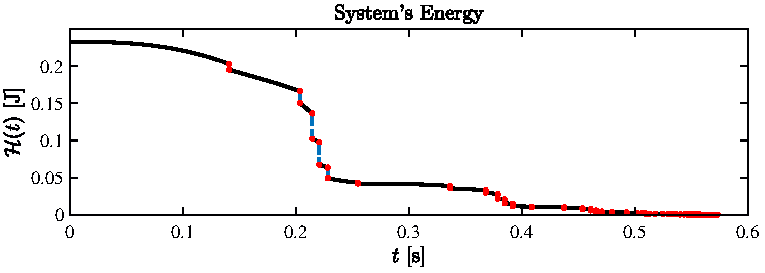
\includegraphics[width=\linewidth]{Figures/aut3.pdf}
%	\caption[Uncontrolled system: time evolution of the Hamiltonian function]{Uncontrolled system: time evolution of the Hamiltonian function. Due to system's passivity, the energy monotonically decreases to zero both during flow and jumps.}
%	\label{fig:aut3}
%\end{figure}
%%
%\begin{figure}[!ht]
%	\centering
%	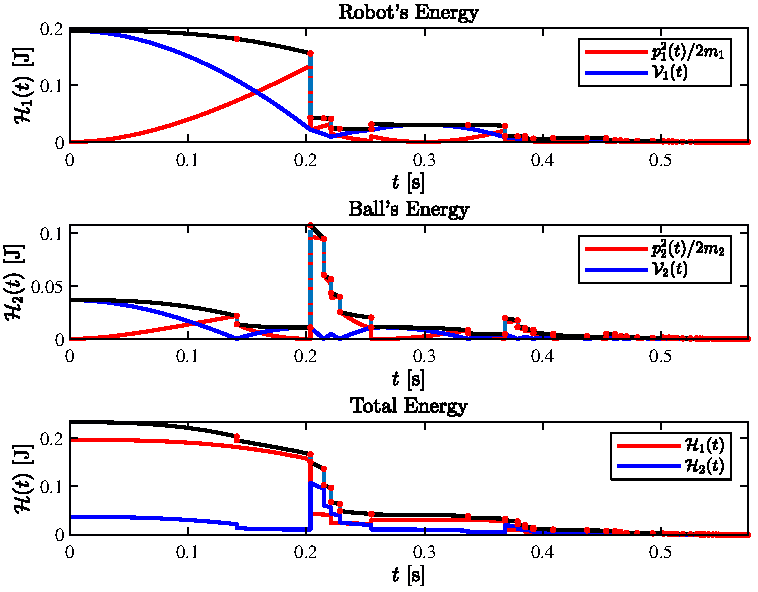
\includegraphics[width=\linewidth]{Figures/aut4.pdf}
%	\caption[Uncontrolled system: Energy distribution within the system]{Uncontrolled system: Energy distribution within the system. Trajectories happen on decreasing level--sets of $\Ha$, even if $\Ha_1$ and $\Ha_2$ may locally increase after some ball--robot impacts.}
%	\label{fig:aut4}
%\end{figure}
%%
%%
%It can be noticed that $\Ha$ presents a monotonically decreasing trend, in both flows (due to the viscous friction terms) and jumps (since the restitution coefficients are less than one). In fact, trajectories happen on decreasing level--sets of $\Ha$, even if $\Ha_1$ and $\Ha_2$ may locally increase after some ball--robot impacts. Moreover, from the figures it is easily to verify the asymptotic stability and attractivity of the origin ($x = \mymathbb{0}_4$) and the \textit{Zeno behavior} of the autonomous system (see \cite{goebel2009hybrid}).
%%%%%%%%%%%%%%%%%%%%%%%%%%%%%%%
%\subsection{Controlled System}\label{sec:controlled_bd}
%%
%Simulations of the system controlled via iterative energy shaping have also been performed. The control parameters have been chosen as: $k_{p,w} = 10^4$, $k_{d,w} = 10^3$, $\delta = 0.05$m, $k_0 = 10$, $k_{d,h} = 0$, $\varphi_\xi(e) = 10e + 100\sum_{i = 1}^{\xi}e(i)$, $q_{2,max}^* = 0.1$m. The time evolution of the state variables are shown in Figs. \ref{fig:ctrl1} and \ref{fig:ctrl1_det}.
%%
%\begin{figure}[!ht]
%	\centering
%	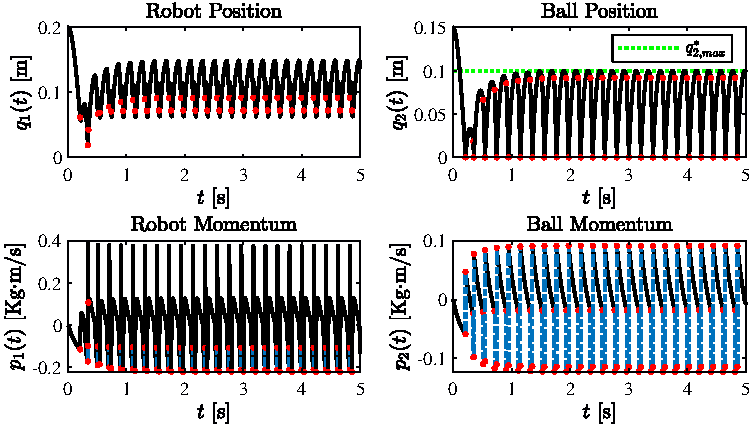
\includegraphics[width=\linewidth]{Figures/ctrl1.pdf}
%	\caption[Iterative energy shaping control: time evolution of the robot and ball states]{Iterative energy shaping control: time evolution of the robot and ball states (position and momentum). Red dots correspond to system's jumps while dashed blue lines highlight discontinuous state changes. Notice that the ball states converge on a periodic trajectory reaching at each bounce the desired peak $q^*_{2,max}$ (dotted green line).}
%	\label{fig:ctrl1}
%\end{figure}
%%
%%
%\begin{figure}[!ht]
%	\centering
%	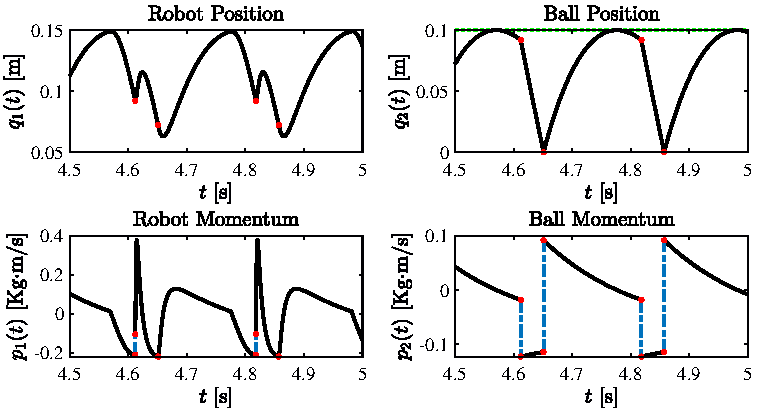
\includegraphics[width=\linewidth]{Figures/ctrl1_det.pdf}
%	\caption[Iterative energy shaping control: detailed view of the time evolution of the ball and robot positions at steady state]{Iterative energy shaping control: detailed view of the time evolution of the ball and robot positions at steady state.}
%	\label{fig:ctrl1_det}
%\end{figure}
%%
%%
%Notice that the trajectory of the ball becomes periodic (asymptotically), reaching at each bounce the desired peak $q_{2,max}^*$, proving the effectiveness of the proposed control scheme. Furthermore, the time evolution of the energy function is shown in Figs. \ref{fig:ctrl3} and \ref{fig:ctrl3_det} while Figs. \ref{fig:ctrl4} and \ref{fig:ctrl4_det} show how the energy flows across the system during each period. 
%%
%\begin{figure}[!ht]
%	\centering
%	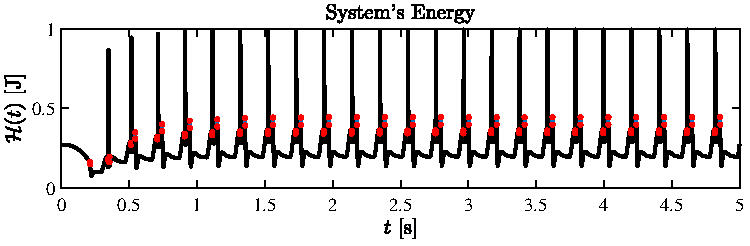
\includegraphics[width=\linewidth]{Figures/ctrl3.pdf}
%	\caption[Iterative energy shaping control: the time evolution of the Hamiltonian function]{Iterative energy shaping control: the time evolution of the Hamiltonian function. After a short transient also the system's energy becomes periodic.}
%	\label{fig:ctrl3}
%\end{figure}
%%
%\begin{figure}[!ht]
%	\centering
%	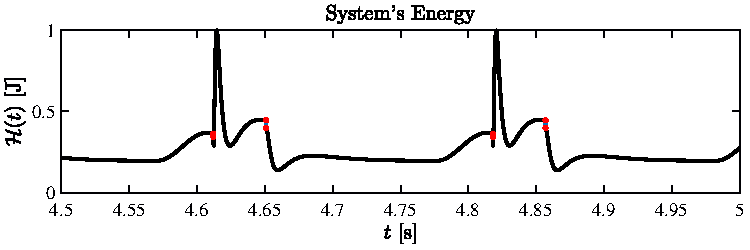
\includegraphics[width=\linewidth]{Figures/ctrl3_det.pdf}
%	\caption[Iterative energy shaping control: detailed view of the the Hamiltonian at steady--state]{Iterative energy shaping control: detailed view of the time evolution of the Hamiltonian function at steady--state to highlight its (asymptotic) periodicity.}
%	\label{fig:ctrl3_det}
%\end{figure}
%%
%\begin{figure}[!ht]
%	\centering
%	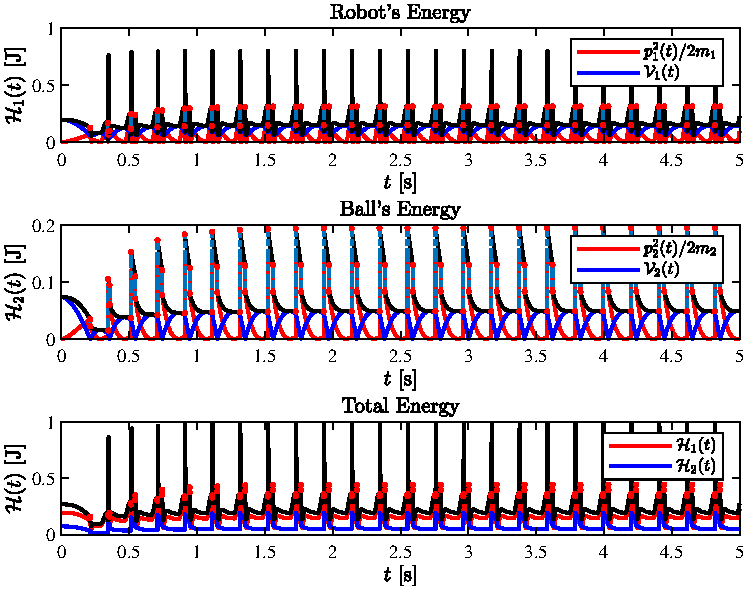
\includegraphics[width=\linewidth]{Figures/ctrl4.pdf}
%	\caption[Iterative energy shaping control: Distribution of the energy across the system's components and time]{Iterative energy shaping control: Distribution of the energy across the system's components and time. After a short transient also the system's energy becomes periodic.}
%	\label{fig:ctrl4}
%\end{figure}
%%
%\begin{figure}[!ht]
%	\centering
%	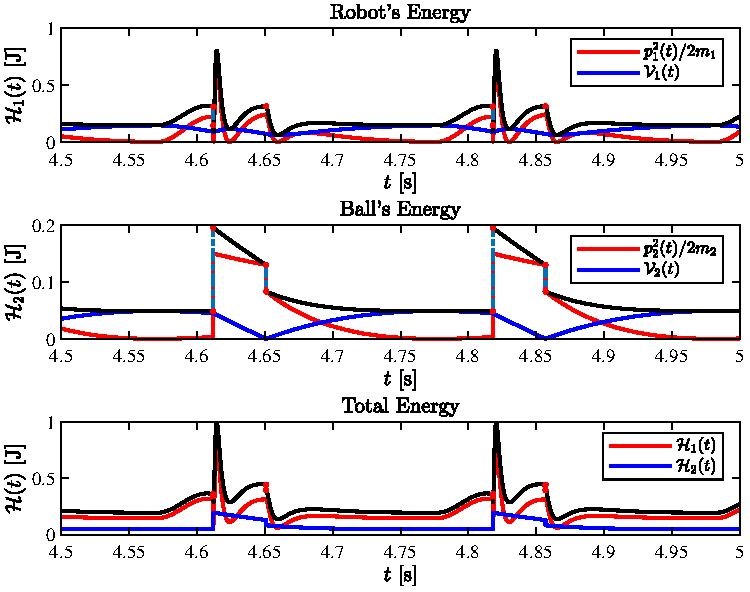
\includegraphics[width=\linewidth]{Figures/ctrl4_det.pdf}
%	\caption[Iterative energy shaping control: detailed view of the energy distribution across the system's components and time]{Iterative energy shaping control: detailed view of the energy distribution across the system's components and time. at steady state to highlight its (asymptotic) periodicity.}
%	\label{fig:ctrl4_det}
%\end{figure}
%%
%As expected also the energy becomes periodic. In fact, the energy at the beginning and at the end of each cycle (bounce) become exactly the same. Moreover, we can see that, at steady state, during the ball--robot impact, the robot transfers to the ball the exact amount of energy necessary to reach the desired bounce peak. Finally, as shown in Fig. \ref{fig:ctrl5} the error goes to zero with the number of cycles.
%%
%\begin{figure}[!ht]
%	\centering
%	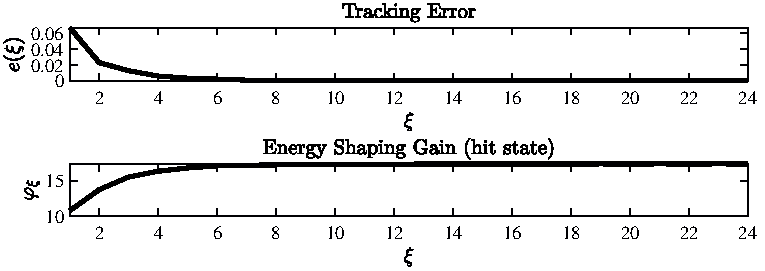
\includegraphics[width=\linewidth]{Figures/ctrl5.pdf}
%	\caption[Iterative energy shaping control: (discrete) time evolution of the tracking error $e$ and of the energy shaping gain $\varphi_\xi(e)$]{Iterative energy shaping control: (discrete) time evolution of the tracking error $e$ and of the energy shaping gain $\varphi_\xi(e)$. As the number of cycles $\xi$ increases, the tracking error $e$, i.e. the difference between the desired and ball's bounce peak, goes asymptotically to zero. Instead, the energy shaping gain converges, increasing monotonically, to a constant value.}
%	\label{fig:ctrl5}
%\end{figure}
%%
%On the other hand, the function $\varphi_\xi(e)$ converges exponentially to a positive constant value. 
%%
%A final consideration about the convergence of the system to the desired periodic trajectory can be made from the phase-space portrait of the system's trajectory (Fig. \ref{fig:ctrl2}). Being the time represented by the color transition, it can be noticed that the system approaches a limit cycle, an attractive asymptotically periodic trajectory, in which the tracking error is zero.
%%
%%
%\begin{figure}[!ht]
%	\centering
%	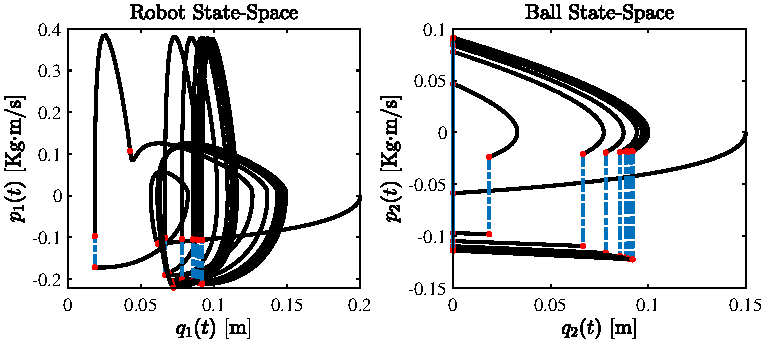
\includegraphics[width=\linewidth]{Figures/ctrl2.pdf}
%	\caption[Iterative energy shaping control: phase--space trajectories]{Iterative energy shaping control: projections on the $q_1-p_1$ plane (above) and the $q_2-p_2$ plane (below) of the phase-space trajectory of the system. The system converges to a hybrid limit cycle in which $e=0$.}
%	\label{fig:ctrl2}
%\end{figure}
%%
%\clearpage
%%
%\subsection{Numerical Stability and Robustnes Analysis}
%%
%\subsubsection{Robustness to Initial Condition}
%In order to prove numerically the stability and robustness of the proposed control scheme, a Monte Carlo experiment similar to the one in Section \ref{sec:analysis_aut}, has been performed. In particular, choosing as physical parameters $m_1=0.1\text{Kg}$, $m_2=0.15\text{Kg}$, $\beta_1=0.2$, $\beta_2=0.3$, $c_1=c_2=0.8$ and control parameters $k_{p,w} = 10^4$, $k_{d,w} = 10^3$, $\delta = 0.5$, $\sigma = 10$, $k_{d,h} = 10^2$, $\varphi_\xi(e) = 3000 + 10e + 300\sum_{i = 1}^{\xi}e(i)$, $q_{2,max}^* = 1$, a total of 3000 trajectories has been computed starting from initial conditions $\xb_0^i$ sampled by the normal distribution
%%
%\begin{equation}
%    \N(\xb_0,\sigma\mathbb{I}_n),
%\end{equation}
%%
%with $\xb_0\triangleq(2,1.5,0,0)$ and $\sigma=1$\footnote{The reason why we chose larger physical and control parameters with respect to the one used in the previous section is that we wanted to minimize the effects of numerical instabilities of the \textit{HyEq} solver}. The time evolution of the system's state in the nominal case ($\xb(t=0) = \xb_0$) and all the Monte Carlo trials are displayed in Fig. \ref{fig:reg1}.
%%
%\begin{figure}[!ht]
%    \centering
%    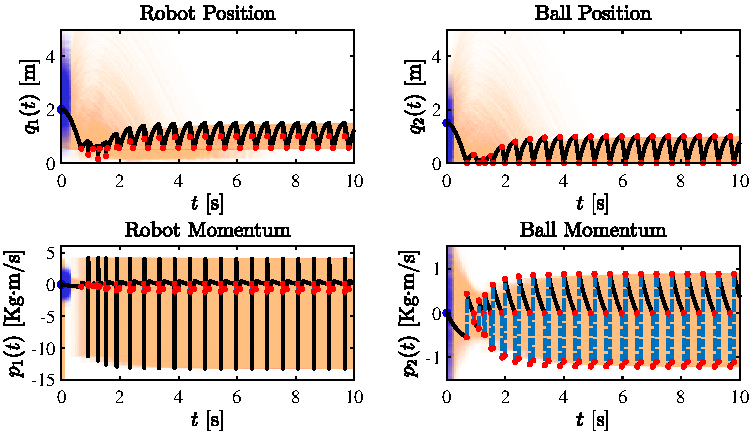
\includegraphics[width = \linewidth]{Figures/reg1.pdf}
%    \caption[Time evolution of the controlled system' state in the Monte Carlo simulation]{Time evolution of the controlled system' state in the Monte Carlo simulation. The black trajectory is the nominal one (starting from $\xb_0$), where red dots and dashed blue lines indicate discrete events (impacts) and the value of the state after the events, respectively. Orange lines show the traces of all the other trajectories of the Monte Carlo runs (with initial condition sampled from $\N(\xb_0,\sigma\mathbb{I}_n)$). The blue dots at $t=0$ are the initial conditions. It can be noticed how trajectories, starting far from each other, eventually converge to the nominal trajectory.}
%    \label{fig:reg1}
%\end{figure}
%%
%It can be noticed how trajectories, starting far from each other, are all asymptotically periodic and eventually converge to the nominal trajectory. This means that the controller generates an attractive \textit{limit cycle} in the closed--loop system. This is further highlighted in Fig. \ref{fig:reg2} where the phase--space trajectories are represented.
%%
%\begin{figure}[!ht]
%    \centering
%    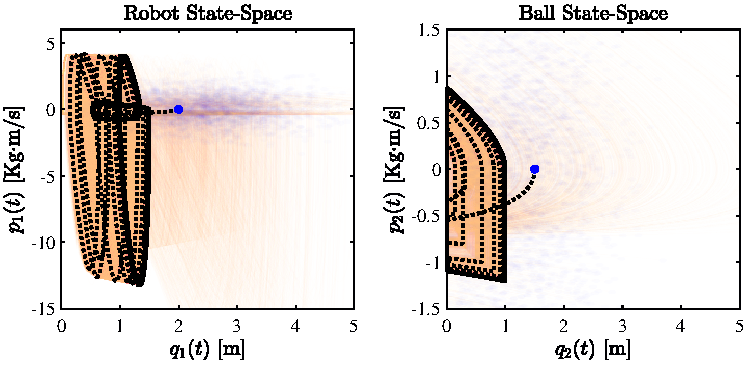
\includegraphics[width = \linewidth]{Figures/reg2.pdf}
%    \caption[Phase--space trajectory of the controlled system in the Monte Carlo simulation]{Phase--space trajectory of the controlled system in the Monte Carlo simulation. The dashed black line is the nominal one (starting from $\xb_0$). Orange lines show the traces of all the other trajectories of the Monte Carlo runs (with initial condition sampled from $\N(\xb_0,\sigma\mathbb{I}_n)$). The blue dots at are the initial conditions. It can be noticed how trajectories, starting far from each other, eventually converge to the nominal trajectory.}
%    \label{fig:reg2}
%\end{figure}
%%
%\vspace{-5mm}
%\begin{figure}[!ht]
%    \centering
%    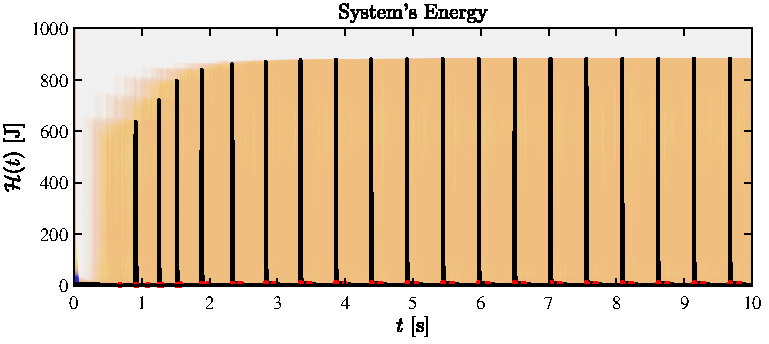
\includegraphics[width = \linewidth]{Figures/reg3.pdf}
%    \caption[Time evolution of the energy in the Monte Carlo simulation]{Time evolution of the energy in the Monte Carlo simulation. The black trajectory is the nominal one (starting from $\xb_0$), where red dots indicate discrete events (impacts). Orange lines show the traces of all the other trajectories of the Monte Carlo runs (with initial condition sampled from $\N(\xb_0,\sigma\mathbb{I}_n)$). The blue dots at $t=0$ are the initial energies of each Monte Carlo run.}
%    \label{fig:reg3}
%\end{figure}
%
%The time evolution of the energy (Hamiltonian function) among the Monte Carlo runs is also shown in Fig. \ref{fig:reg3}.
%
%A final results to show stability and attractivity to the nominal trajectory of the iterative energy shaping controlled system is the convergence of the tracking error and energy shaping gain, reported in Fig. \ref{fig:reg4}.  It is worth to be notices that the mean the both the error and gain among the Monte Carlo runs is almost identical to the nominal one. Further investigations might be interesting to be carried out to discover the source os this phenomenon.
%%
%\begin{figure}[!ht]
%	\centering
%	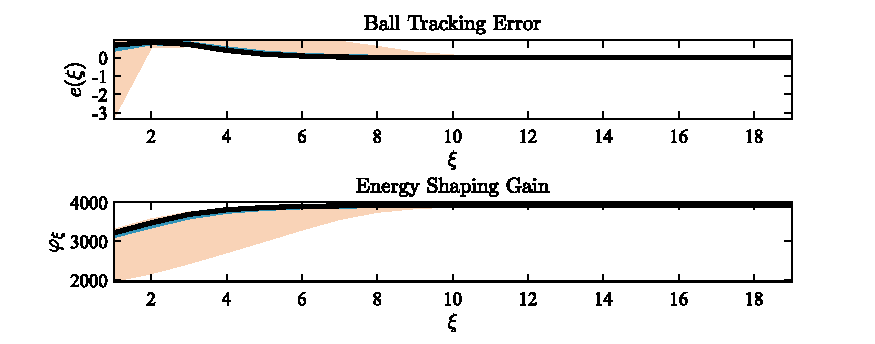
\includegraphics[width = \linewidth]{Figures/reg4.pdf}
%	\caption[Convergence of the tracking error and controller gain in the Monte Carlo simulation]{Convergence of the tracking error and energy shaping gain (hit state) in the Monte Carlo simulation. The black line indicates the nominal case. The orange area bounds the minimum and maximum among the values of each Monte Carlo runs while the blue line is their average.}
%	\label{fig:reg4}
%\end{figure}
%%
%\subsubsection{Robustness to Change of Parameters}
%%
%To prove the robustness against sudden changes of physical parameters of the system, several simulations has been performed with the same model and control parameters as in Subsection \ref{sec:controlled_bd} changing at time $t = 2.5s$ some parameter of the model. First we tried to change the reference from $0.1$m to $0.05$m (-50\%). Then, the mass of the ball $m_2$ has been change from $0.05$Kg to $0.25$Kg (+400\%). Finally, the restitution coefficient of the ball--robot collision has been changed from $0.8$ to $0.99$ (+23.75\%). The resulting states trajectories, tracking error, learned gains and energy are reported in Figs. \ref{fig:roba}, \ref{fig:robb} and \ref{fig:robc}.
%% 
%\begin{figure}[!ht]
%	\centering
%	\subfigure[States time evolution]{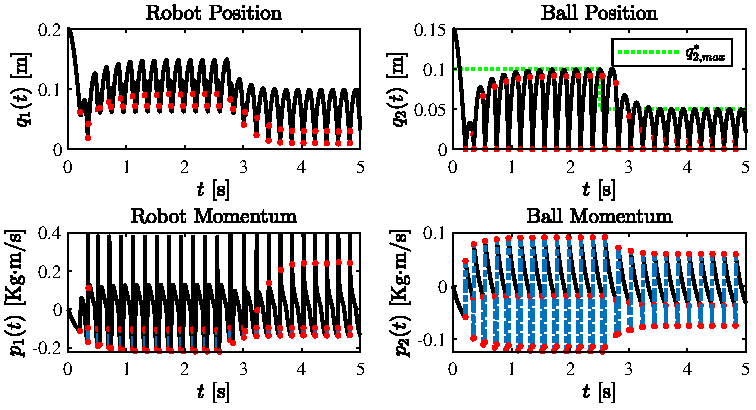
\includegraphics[width=.8\linewidth]{Figures/rob1.pdf}}
%	\subfigure[Tracking error and learned gain]{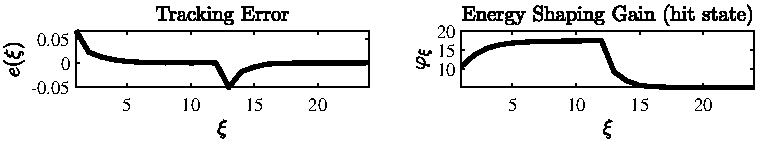
\includegraphics[width=.8\linewidth]{Figures/rob2l.pdf}}
%	\subfigure[System's energy]{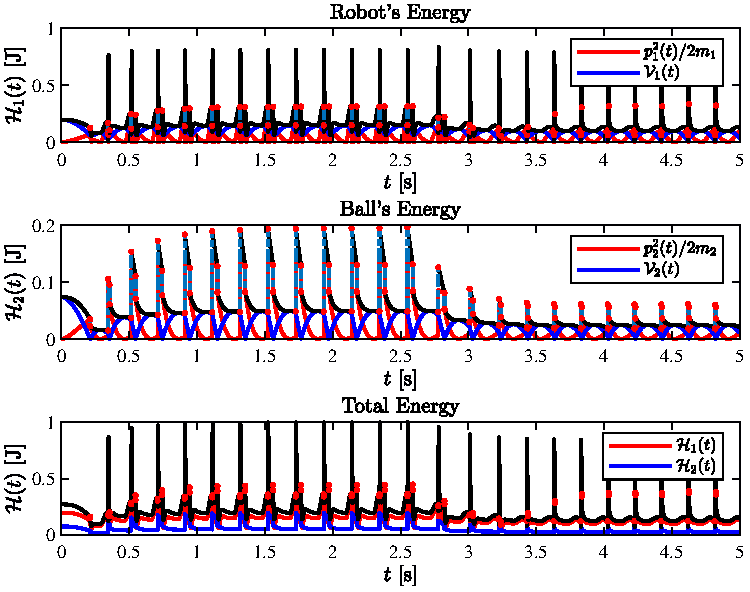
\includegraphics[width=.8\linewidth]{Figures/rob3.pdf}}
%	\caption[Robustness to parameters variations: reference position]{Robustness to parameters variations: reference position.}
%	\label{fig:roba}
%\end{figure}
%%
%\begin{figure}[!ht]
%	\centering
%	\subfigure[States time evolution]{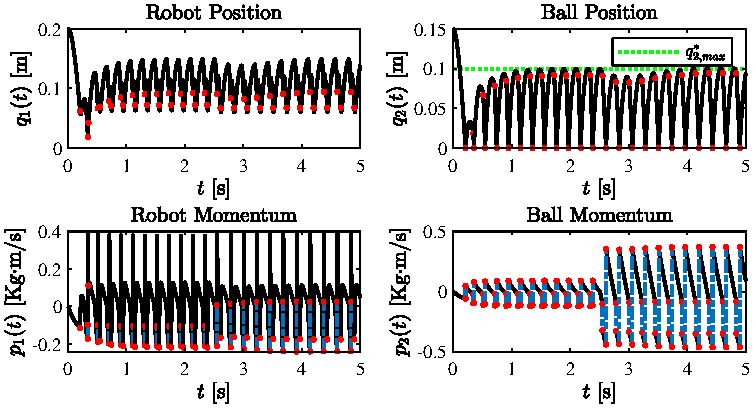
\includegraphics[width=.8\linewidth]{Figures/rob4.pdf}}
%	\subfigure[Tracking error and learned gain]{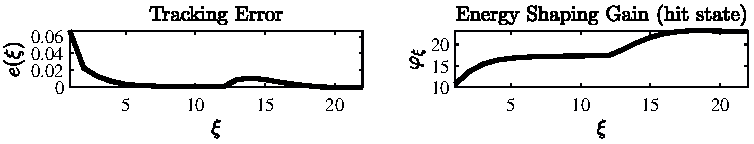
\includegraphics[width=.8\linewidth]{Figures/rob5l.pdf}}
%	\subfigure[System's energy]{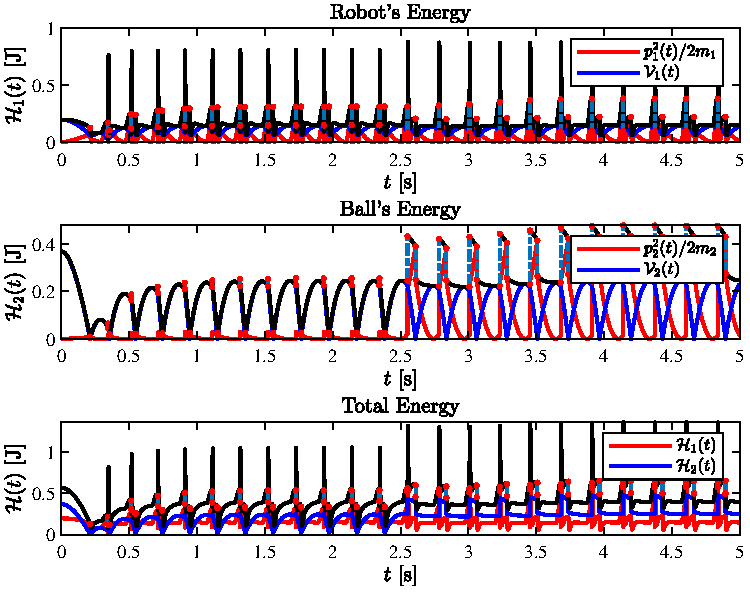
\includegraphics[width=.8\linewidth]{Figures/rob6.pdf}}
%	\caption[Robustness to parameters variations: ball's mass]{Robustness to parameters variations: ball's mass.}
%	\label{fig:robb}
%\end{figure}
%%
%\begin{figure}[!ht]
%	\centering
%	\subfigure[States time evolution]{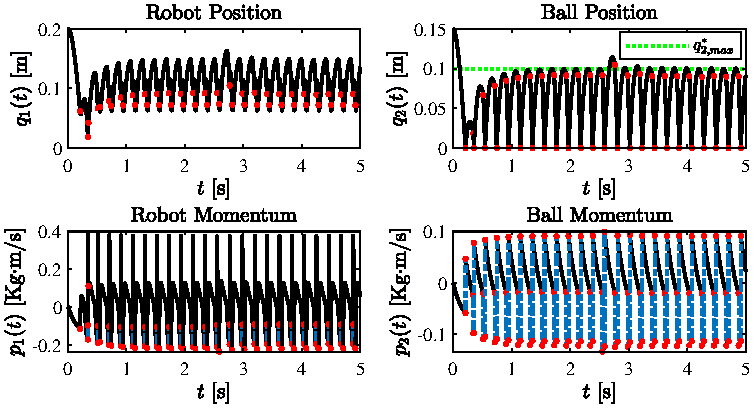
\includegraphics[width=.8\linewidth]{Figures/rob7.pdf}}
%	\subfigure[Tracking error and learned gain]{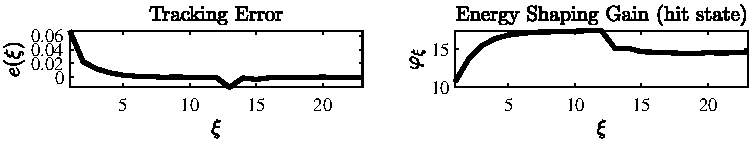
\includegraphics[width=.8\linewidth]{Figures/rob8l.pdf}}
%	\subfigure[System's energy]{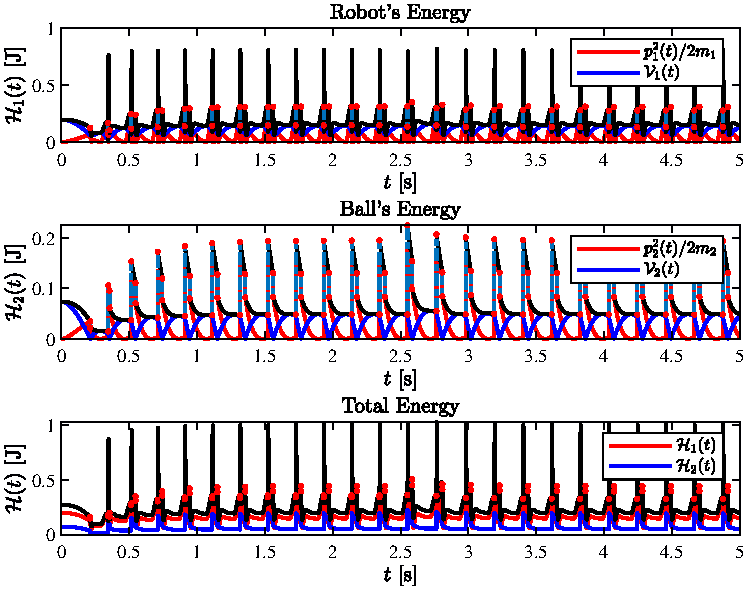
\includegraphics[width=.8\linewidth]{Figures/rob9.pdf}}
%	\caption[Robustness to parameters variations: restitution coefficients]{Robustness to parameters variations: restitution coefficients.}
%	\label{fig:robc}
%\end{figure}
%%
%
%The controller shows excellent robustness properties. In all three situations, the system recovers swiftly from the parameter change, adapting to the new value. 
%
%In particular, when the reference is changed from $0.1$m to $0.05$m, all the physical properties of the system are conserved, e.g. dissipation during flows and jumps. However the robot needs to transfer less momentum to the ball during their collision to stabilize the ball on the desired trajectory. The system thus adapts by decreasing the energy shaping gain in the hit state. 
%
%Instead, when the mass of the ball is increased from $0.05$Kg to $0.25$Kg, its momentum per unit of speed grows and thus, the conservation of momentum during the ball--robot collision implies that the robot needs more speed to transfer the same momentum to the ball. In turn, the acceleration of the robot during the hit mode is also controlled by the energy shaping gain. Consequently, it automatically adapts increasing towards the value of zero tracking error.
%
%Finally, when the the ball--robot collision's restitution coefficient is increased from 0.8 to 0.99, the percentage of momentum that the robot transfers to the ball, i.e elasticity of impact, increases. Consequently, the energy shaping gain lowers.    
%%
%Robustness to changes in the robot mass, friction coefficients and ball--ground restitution coefficients have also been tested, obtaining good results.
\subsection{Autonomous System}
%
Firstly, the behavior of the uncontrolled system has been simulated. The time evolution of the state variables are shown in Fig.~\ref{fig:aut1}.
%
\begin{figure}[ht!]
	\centering
	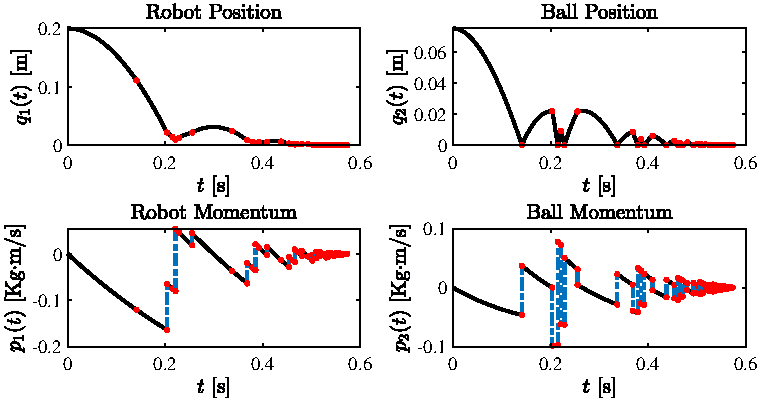
\includegraphics[width = \linewidth]{Figures/aut1.pdf}
	\caption[Uncontrolled system: time evolution of the robot and ball position states]{Uncontrolled system: time evolution of the robot and ball position states (position and momentum). Red dots correspond to system's jumps while dashed blue lines highlight discontinuous state changes. Notice that both the position and velocity go asymptotically to zero.}
	\label{fig:aut1}
\end{figure}
%
The phase--space trajectory of the autonomous system over the energy of the system is represented in Fig.~\ref{fig:aut2}. 
%
\begin{figure}[hb!]
	\centering
	\definecolor{ocean}{rgb}{0.00000,0.44700,0.74100}
\definecolor{mycolor1}{rgb}{0.00000,0.44700,0.74100}%

\begin{tikzpicture}
\begin{axis}[
width=5cm,
height=5cm,
at={(1in,0.331in)},
view={0}{90},
colorbar horizontal,
colormap = {whiteblack}{color(0cm)  = (white);color(1cm) = (black)},
colorbar style = {at = {(0,-0.25)}},
xmin=0,
xmax=.2,
xlabel style={font=\color{white!15!black},at = {(0.75in,-0.125in)}},
xlabel={$q_1(t)~[m]$},
ymin=-.2,
ymax=.1,
ylabel style={font=\color{white!15!black},at = {(-0.1in,0.75in)}},
ylabel={$p_1(t)~$[Kg$\cdot$m/s]},
title = {robot phase--space},
axis background/.style={fill=white},
]
\addplot3[contour filled={number = 25,labels={false}},mesh/rows=25,mesh/cols=25,mesh/check=false,forget plot
] table {H1_a.dat};
%%%%%%%%%%%%%%%%%%%%%%%%%%%%%%%%%%%%
\addplot [color=black, line width=1.5pt]
  table[row sep=crcr]{%
0.2	0\\
0.2	0\\
0.199999967381998	-7.99934763995355e-05\\
0.199998826071083	-0.000479765214216573\\
0.199989131483394	-0.00145882629667888\\
0.199969656068965	-0.00243593121379302\\
0.1999404193699	-0.00341108387397995\\
0.199901440889258	-0.00438428817785163\\
0.199852740091133	-0.00535554801822656\\
0.199794336400727	-0.00632486728014541\\
0.199726249204433	-0.00729224984088653\\
0.199648497849907	-0.00825769956998144\\
0.199561101646152	-0.00922122032923035\\
0.199464079863588	-0.0101828159727176\\
0.199357451734135	-0.011142490346827\\
0.199241236451287	-0.0121002472902574\\
0.199115453170189	-0.0130560906340378\\
0.198980121007714	-0.0140100242015429\\
0.198835259042541	-0.0149620518085082\\
0.198680886315227	-0.0159121772630453\\
0.198517021828288	-0.0168604043656575\\
0.198343684546272	-0.0178067369092544\\
0.198160893395837	-0.0187511786791674\\
0.197968667265824	-0.0196937334531649\\
0.197767025007336	-0.0206344050014671\\
0.197555985433808	-0.0215731970867617\\
0.19733556732109	-0.0225101134642181\\
0.197105789407515	-0.0234451578815031\\
0.196866670393978	-0.0243783340787956\\
0.196618228944009	-0.0253096457888017\\
0.196360483683848	-0.0262390967367695\\
0.19609345320252	-0.027166690640504\\
0.19581715605191	-0.028092431210382\\
0.195531610746835	-0.0290163221493671\\
0.195236835765121	-0.0299383671530242\\
0.194932849547673	-0.0308585699095347\\
0.194619670498553	-0.0317769340997106\\
0.194297316985051	-0.0326934633970102\\
0.193965807337758	-0.0336081614675517\\
0.193625159850643	-0.0345210319701286\\
0.193275392781121	-0.0354320785562243\\
0.192916524350131	-0.0363413048700261\\
0.192548572742204	-0.0372487145484408\\
0.19217155610554	-0.038154311221108\\
0.191785492552079	-0.0390580985104158\\
0.191390400157573	-0.0399600800315146\\
0.190986296961657	-0.0408602593923315\\
0.190573200967926	-0.0417586401935853\\
0.190151130144001	-0.0426552260288003\\
0.189720102421606	-0.0435500204843211\\
0.189280135696634	-0.0444430271393267\\
0.188831247829225	-0.045334249565845\\
0.188373456643834	-0.0462236913287668\\
0.187906779929302	-0.0471113559858603\\
0.187431235438927	-0.0479972470877854\\
0.186946840890538	-0.0488813681781077\\
0.186453613966563	-0.0497637227933127\\
0.1859515723141	-0.05064431446282\\
0.185440733544988	-0.0515231467089975\\
0.184921115235877	-0.0524002230471754\\
0.184392734928301	-0.0532755469856602\\
0.183855610128744	-0.0541491220257488\\
0.183309758308713	-0.0550209516617425\\
0.182755196904805	-0.0558910393809611\\
0.182191943318783	-0.0567593886637566\\
0.181620014917636	-0.0576260029835272\\
0.181039429033657	-0.0584908858067314\\
0.180450202964509	-0.0593540405929017\\
0.179852353973292	-0.0602154707946584\\
0.179245899288617	-0.0610751798577234\\
0.17863085610467	-0.0619331712209341\\
0.178007241581285	-0.0627894483162571\\
0.17737507284401	-0.0636440145688019\\
0.176734366984174	-0.0644968733968348\\
0.17608514105896	-0.0653480282117921\\
0.175427412091471	-0.0661974824182942\\
0.174761197070796	-0.0670452394141591\\
0.17408651295208	-0.067891302590416\\
0.173403376656593	-0.0687356753313186\\
0.172711805071795	-0.0695783610143591\\
0.172011815051406	-0.0704193630102812\\
0.171303423415471	-0.0712586846830942\\
0.170586646950429	-0.0720963293900858\\
0.16986150240918	-0.072932300481836\\
0.169128006511151	-0.0737666013022302\\
0.168386175942364	-0.0745992351884729\\
0.167636027355503	-0.0754302054711006\\
0.166877577369979	-0.0762595154739958\\
0.166110842571997	-0.0770871685143994\\
0.165335839514624	-0.0779131679029247\\
0.164552584717852	-0.0787375169435705\\
0.163761094668669	-0.0795602189337339\\
0.16296138582112	-0.080381277164224\\
0.162153474596374	-0.0812006949192748\\
0.161337377382792	-0.0820184754765585\\
0.160513110535992	-0.0828346221071984\\
0.15968069037891	-0.083649138075782\\
0.158840133201872	-0.0844620266403744\\
0.157991455262655	-0.0852732910525309\\
0.157134672786551	-0.0860829345573103\\
0.156269801966437	-0.0868909603932875\\
0.155396858962835	-0.0876973717925671\\
0.154515859903979	-0.0885021719807957\\
0.153626820885876	-0.0893053641771752\\
0.152729757972377	-0.0901069515944754\\
0.151824687195235	-0.090906937439047\\
0.150911624554173	-0.0917053249108346\\
0.149990586016945	-0.092502117203389\\
0.149061587519402	-0.0932973175038804\\
0.148124644965556	-0.0940909289931113\\
0.147179774227642	-0.0948829548455284\\
0.146226991146182	-0.0956733982292365\\
0.145266311530049	-0.0964622623060099\\
0.144297751156531	-0.0972495502313062\\
0.14332132577139	-0.0980352651542779\\
0.14233705108893	-0.098819410217786\\
0.141344942792058	-0.0996019885584117\\
0.140345016532346	-0.100383003306469\\
0.139337287930095	-0.101162457586019\\
0.138321772574394	-0.101940354514879\\
0.137298486023188	-0.102716697204638\\
0.136267443803336	-0.103491488760667\\
0.135228661410673	-0.104264732282135\\
0.134182154310077	-0.105036430862015\\
0.133127937935522	-0.105806587587104\\
0.13206602769015	-0.10657520553803\\
0.130996438946323	-0.107342287789265\\
0.129919187045693	-0.108107837409139\\
0.128834287299257	-0.108871857459852\\
0.127741754987421	-0.109634350997484\\
0.12664160536006	-0.110395321072012\\
0.125533853636582	-0.111154770727317\\
0.124418515005985	-0.111912703001197\\
0.123295604626918	-0.112669120925384\\
0.122165137627746	-0.113424027525549\\
0.121027129106605	-0.114177425821321\\
0.119881594131468	-0.114929318826294\\
0.118728547740197	-0.11567970954804\\
0.117568004940614	-0.116428600988123\\
0.116399980710552	-0.117175996142111\\
0.115224489997919	-0.117921897999584\\
0.114041547720758	-0.118666309544152\\
0.112851168767303	-0.119409233753461\\
0.111653367996044	-0.120150673599209\\
0.111003126035683	-0.120550649027536\\
};

\addplot [color=black, line width=1.5pt]
  table[row sep=crcr]{%
0.111003126035683	-0.120550649027536\\
0.111003126035683	-0.120550649027536\\
0.110873945268924	-0.120629901224444\\
0.110226768466994	-0.121025907615357\\
0.109012817113077	-0.121764117344574\\
0.107791491039044	-0.122500852129767\\
0.106562804979595	-0.123236114917877\\
0.105326773639992	-0.123969908649957\\
0.104083411696113	-0.124702236261181\\
0.102832733794515	-0.125433100680861\\
0.101574754552493	-0.126162504832457\\
0.100309488558133	-0.126890451633585\\
0.0990369503703772	-0.127616943996034\\
0.0977571545190772	-0.128341984825774\\
0.0964701155050545	-0.129065577022969\\
0.0951758478001579	-0.12978772348199\\
0.0938743658473213	-0.130508427091422\\
0.0925656840606218	-0.131227690734083\\
0.0912498168253371	-0.131945517287026\\
0.0899267784980029	-0.132661909621559\\
0.0885965834064708	-0.133376870603252\\
0.0872592458499652	-0.134090403091951\\
0.0859147800991405	-0.134802509941786\\
0.0845632003961387	-0.135513194001186\\
0.0832045209546456	-0.136222458112887\\
0.0818387559599481	-0.136930305113948\\
0.0804659195689911	-0.137636737835756\\
0.0790860259104336	-0.138341759104045\\
0.0776990890847058	-0.139045371738899\\
0.076305123164065	-0.139747578554771\\
0.0749041421926524	-0.140448382360489\\
0.0734961601865485	-0.141147785959268\\
0.0720811911338302	-0.141845792148724\\
0.0706592489946258	-0.142542403720883\\
0.0692303477011715	-0.143237623462193\\
0.0677945011578667	-0.143931454153532\\
0.0663517232413299	-0.144623898570224\\
0.0649020278004541	-0.145314959482049\\
0.063445428656462	-0.146004639653251\\
0.0619819396029617	-0.146692941842551\\
0.0605115744060017	-0.147379868803159\\
0.0590343468041257	-0.148065423282783\\
0.0575502705084279	-0.148749608023644\\
0.0560593592026076	-0.14943242576248\\
0.0545616265430243	-0.150113879230563\\
0.0530570861587518	-0.150793971153709\\
0.0515457516516331	-0.151472704252285\\
0.0500276365963347	-0.152150081241225\\
0.048502754540401	-0.152826104830038\\
0.0469711190043082	-0.15350077772282\\
0.0454327434815187	-0.154174102618262\\
0.0438876414385349	-0.154846082209665\\
0.0423358263149532	-0.155516719184949\\
0.0407773115235174	-0.156186016226662\\
0.0392121104501729	-0.156853976011993\\
0.03764023645412	-0.157520601212782\\
0.0360617028678669	-0.158185894495532\\
0.0344765229972839	-0.158849858521415\\
0.0328847101216559	-0.159512495946289\\
0.0312862774937359	-0.160173809420705\\
0.0296812383397976	-0.160833801589918\\
0.028069605859689	-0.161492475093896\\
0.0264513932268845	-0.162149832567335\\
0.0248266135885379	-0.162805876639666\\
0.0231952800655351	-0.163460609935065\\
0.0219480095000046	-0.163958559802086\\
};
%\addlegendentry{data2}

\addplot [color=mycolor1, dashdotted, line width=1pt, mark size=0.5pt, mark=*, mark options={solid, fill=red, red}]
  table[row sep=crcr]{%
0.111003126035683	-0.120550649027536\\
0.111003126035683	-0.120550649027536\\
};
%\addlegendentry{data3}

\addplot [color=black, line width=1.5pt]
  table[row sep=crcr]{%
0.0219480096000046	-0.065408056320056\\
0.0219480096000046	-0.065408056320056\\
0.0213610862698025	-0.0661658766261791\\
0.0206951869912011	-0.0670136967704588\\
0.0200208179837062	-0.0678598229689598\\
0.0193379961698475	-0.0687042586061881\\
0.0186467384383433	-0.0695470070598872\\
0.0179470616441683	-0.0703880717010522\\
0.017238982608621	-0.0712274558939427\\
0.0165225181193908	-0.0720651629960967\\
0.0157976849306254	-0.0729011963583436\\
0.0150644997629975	-0.0737355593248181\\
0.0143229793037722	-0.074568255232973\\
0.0140822597838371	-0.0748362274183675\\
};
%\addlegendentry{data4}

\addplot [color=mycolor1, dashdotted, line width=1pt, mark size=0.5pt, mark=*, mark options={solid, fill=red, red}]
  table[row sep=crcr]{%
0.0219480095000046	-0.163958559802086\\
0.0219480096000046	-0.065408056320056\\
};
%\addlegendentry{data5}

\addplot [color=black, line width=1.5pt]
  table[row sep=crcr]{%
0.0140822597838371	-0.0748362274183675\\
0.0140822597838371	-0.0748362274183675\\
0.014043800523677	-0.0748789359842696\\
0.0138511751519139	-0.0750924129995873\\
0.013096099715432	-0.0759223979122909\\
0.0123327327241388	-0.0767507245140323\\
0.0115610907445722	-0.077577396118119\\
0.0107811903101695	-0.0784024160312385\\
0.00999304792133467	-0.0792257875534715\\
0.00928590400525915	-0.0799559502607498\\
};
%\addlegendentry{data6}

\addplot [color=mycolor1, dashdotted, line width=1pt, mark size=0.5pt, mark=*, mark options={solid, fill=red, red}]
  table[row sep=crcr]{%
0.0140822597838371	-0.0748362274183675\\
0.0140822597838371	-0.0748362274183675\\
};
%\addlegendentry{data7}

\addplot [color=black, line width=1.5pt]
  table[row sep=crcr]{%
0.00928590410525915	0.0544550947842129\\
0.00928590410525915	0.0544550947842129\\
0.00960822168881119	0.0538065018345354\\
0.0101408472708482	0.0527189767181279\\
0.0106626084697222	0.0516336244783532\\
0.0111735269924851	0.0505504407738006\\
0.0116736245028183	0.0494694212717339\\
0.012162922621119	0.0483905616480738\\
0.012641442924587	0.0473138575873802\\
0.0130153166228394	0.0464568105343072\\
};
%\addlegendentry{data8}

\addplot [color=mycolor1, dashdotted, line width=1pt, mark size=0.5pt, mark=*, mark options={solid, fill=red, red}]
  table[row sep=crcr]{%
0.00928590400525915	-0.0799559502607498\\
0.00928590410525915	0.0544550947842129\\
};
%\addlegendentry{data9}

\addplot [color=black, line width=1.5pt]
  table[row sep=crcr]{%
0.0130153166228394	0.0464568105343072\\
0.0130153166228394	0.0464568105343072\\
0.0130520250736697	0.0463718829387801\\
0.0132345600994249	0.0459474464068239\\
0.0136886736653454	0.0448756236936398\\
0.0141320797152157	0.0438059424836657\\
0.0145647996426671	0.0427383984981754\\
0.0149868547985866	0.0416729874669916\\
0.0153982664912017	0.0406097051284685\\
0.0157990559861665	0.0395485472294756\\
0.0161892445066459	0.0384895095253797\\
0.0165688532334012	0.0374325877800286\\
0.0169379033048743	0.036377777765734\\
0.0172964158172725	0.0353250752632544\\
0.0176444118246529	0.0342744760617783\\
0.0179819123390066	0.0332259759589075\\
0.0183089383303426	0.0321795707606403\\
0.0186255107267718	0.0311352562813545\\
0.0189316504145909	0.0300930283437907\\
0.0192273782383656	0.0290528827790357\\
0.019512715001014	0.028014815426506\\
0.0197876814638903	0.0269788221339308\\
0.0200522983468671	0.0259448987573354\\
0.0203065863284188	0.0249130411610251\\
0.0205505660457044	0.023883245217568\\
0.0207842580946495	0.0228555068077789\\
0.0210076830300293	0.021829821820703\\
0.0212208613655503	0.0208061861535988\\
0.0214238135739326	0.0197845957119223\\
0.021616560086992	0.0187650464093104\\
0.0216673234911117	0.018487535439195\\
};
%\addlegendentry{data10}

\addplot [color=mycolor1, dashdotted, line width=1pt, mark size=0.5pt, mark=*, mark options={solid, fill=red, red}]
  table[row sep=crcr]{%
0.0130153166228394	0.0464568105343072\\
0.0130153166228394	0.0464568105343072\\
};
%\addlegendentry{data11}

\addplot [color=black, line width=1.5pt]
  table[row sep=crcr]{%
0.0216673235911117	0.0445428893967084\\
0.0216673235911117	0.0445428893967084\\
0.0220002095780532	0.0437364747396123\\
0.0224322355222784	0.0426690695507672\\
0.0228535980815511	0.0416037970389127\\
0.0232643185613285	0.0405406529429573\\
0.0236644182244996	0.039479633010323\\
0.0240539182914703	0.0384207329969289\\
0.0244328399402478	0.0373639486671734\\
0.0248012043065259	0.0363092757939178\\
0.025159032483769	0.0352567101584692\\
0.0255063455232968	0.0342062475505636\\
0.0258431644343686	0.0331578837683492\\
0.026169510184267	0.0321116146183695\\
0.0264854036983819	0.0310674359155466\\
0.0267908658602945	0.030025343483164\\
0.0270859175118602	0.0289853331528509\\
0.0273705794532927	0.0279474007645644\\
0.0276448724432468	0.0269115421665736\\
0.0279088171989011	0.0258777532154427\\
0.0281624343960417	0.0248460297760146\\
0.0284057446691443	0.0238163677213941\\
0.0286387686114568	0.0227887629329316\\
0.0288615267750819	0.0217632113002066\\
0.029074039671059	0.0207397087210111\\
0.0292763277694467	0.0197182511013336\\
0.029468411499404	0.0186988343553421\\
0.0296503112492728	0.0176814544053684\\
0.0298220473666587	0.0166661071818912\\
0.0299836401585132	0.0156527886235203\\
0.0301351098912141	0.0146414946769801\\
0.0302764767906471	0.0136322212970935\\
0.0304077610422866	0.0126249644467656\\
0.0305289827912762	0.0116197200969677\\
0.0306401621425097	0.010616484226721\\
0.0307413191607112	0.00961525282308071\\
0.0308324738705154	0.00861602188111986\\
0.030913646256548	0.00761878740391335\\
0.030984856263505	0.00662354540252195\\
0.0310461237962332	0.00563029189597632\\
0.0310974687198092	0.0046390229112611\\
0.0311389108596196	0.00364973448329904\\
0.0311704700014393	0.00266242265493509\\
0.0311921658915116	0.00167708347692064\\
0.0312040182366266	0.000693713007897637\\
0.0312060467042002	-0.000287692685617093\\
0.0311982709223529	-0.00126713752924764\\
0.0311807104799882	-0.00224462544077469\\
0.0311533849268707	-0.00322016033015118\\
0.0311163137737047	-0.004193746099518\\
0.0310695164922122	-0.0051653866432195\\
0.0310130125152106	-0.00613508584781916\\
0.0309468212366903	-0.00710284759211511\\
0.0308709620118927	-0.0080686757471556\\
0.0307854541573875	-0.00903257417625454\\
0.0306903169511495	-0.00999454673500695\\
0.0305855696326365	-0.0109545972713043\\
0.0304712314028655	-0.0119127296253502\\
0.0303473214244901	-0.0128689476296751\\
0.0302138588218766	-0.0138232551091524\\
0.0300708626811812	-0.0147756558810133\\
0.0299183520504255	-0.0157261537548621\\
0.0297563459395734	-0.0166747525326917\\
0.0295848633206068	-0.0176214560088984\\
0.0294039231276015	-0.0185662679702974\\
0.0292135442568031	-0.0195091921961377\\
0.0290137455667024	-0.0204502324581175\\
0.0288045458781109	-0.0213893925203992\\
0.0285859639742362	-0.0223266761396243\\
0.0283580186007568	-0.0232620870649284\\
0.0281207284658976	-0.0241956290379566\\
0.0278741122405042	-0.0251273057928779\\
0.027618188558118	-0.0260571210564007\\
0.0273529760150504	-0.0269850785477871\\
0.0270784931704575	-0.0279111819788686\\
0.0267947585464141	-0.0288354350540599\\
0.0265017906279878	-0.0297578414703746\\
0.0261996078633131	-0.0306784049174397\\
0.0258882286636652	-0.0315971290775101\\
0.0255676714035334	-0.0325140176254837\\
0.0252379544206947	-0.033429074228916\\
0.0248990960162873	-0.0343423025480345\\
0.0245511144548837	-0.0352537062357538\\
0.024206561480461	-0.03613178120804\\
};
%\addlegendentry{data12}

\addplot [color=mycolor1, dashdotted, line width=1pt, mark size=0.5pt, mark=*, mark options={solid, fill=red, red}]
  table[row sep=crcr]{%
0.0216673234911117	0.018487535439195\\
0.0216673235911117	0.0445428893967084\\
};
%\addlegendentry{data13}

\addplot [color=black, line width=1.5pt]
  table[row sep=crcr]{%
0.024206561480461	-0.03613178120804\\
0.024206561480461	-0.03613178120804\\
0.0241434365718622	-0.0362901693707391\\
0.0238236730155906	-0.0370812823815791\\
0.0234483290273901	-0.037987213583939\\
0.0230639347804385	-0.0388913347345487\\
0.0226705083571647	-0.0397936494498939\\
0.0222680678038693	-0.0406941613392348\\
0.0218566311307959	-0.0415928740046201\\
0.021436216312204	-0.0424897910409018\\
0.0210068412864401	-0.043384916035749\\
0.0205685239560102	-0.044278252569663\\
0.0201212821876509	-0.0451698042159911\\
0.0196651338124011	-0.0460595745409412\\
0.0192000966256733	-0.0469475671035956\\
0.0187261883873246	-0.0478337854559259\\
0.018243426821728	-0.0487182331428066\\
0.0177518296178431	-0.0496009137020296\\
0.0172514144292871	-0.0504818306643184\\
0.016742198874405	-0.051360987553342\\
0.0162242005363405	-0.0522383878857291\\
0.0156974369631062	-0.0531140351710822\\
0.0151619256676535	-0.0539879329119917\\
0.0146176841279432	-0.0548600846040496\\
0.0140647297870148	-0.0557304937358639\\
0.0135030800530569	-0.0565991637890723\\
0.0129327522994763	-0.0574660982383562\\
0.0123537638649678	-0.0583313005514545\\
0.0117661320535834	-0.0591947741891777\\
0.0111698741348017	-0.0600565226054213\\
0.0105650073435967	-0.0609165492471803\\
0.00995154888050709	-0.0617748575545624\\
0.00932951591170463	-0.0626314509608019\\
0.00869892556906321	-0.0634863328922736\\
0.00857212106226058	-0.0636566496567663\\
};
%\addlegendentry{data14}

\addplot [color=mycolor1, dashdotted, line width=1pt, mark size=0.5pt, mark=*, mark options={solid, fill=red, red}]
  table[row sep=crcr]{%
0.024206561480461	-0.03613178120804\\
0.024206561480461	-0.03613178120804\\
};
%\addlegendentry{data15}

\addplot [color=black, line width=1.5pt]
  table[row sep=crcr]{%
0.00857212116226058	-0.0194049517610908\\
0.00857212116226058	-0.0194049517610908\\
0.00839879882932497	-0.0202282951193367\\
0.00819181629622749	-0.0211678986127172\\
0.00797544711796713	-0.0221056247770652\\
0.00774971004907341	-0.0230414773632864\\
0.00751462380660433	-0.0239754601147926\\
0.00727020707022115	-0.024907576767516\\
0.00701647848226316	-0.0258378310499244\\
0.00675345664782221	-0.0267662266830362\\
0.00648116013481716	-0.0276927673804352\\
0.00619960747406817	-0.0286174568482854\\
0.0059965560509815	-0.0292651122340497\\
};
%\addlegendentry{data16}

\addplot [color=mycolor1, dashdotted, line width=1pt, mark size=0.5pt, mark=*, mark options={solid, fill=red, red}]
  table[row sep=crcr]{%
0.00857212106226058	-0.0636566496567663\\
0.00857212116226058	-0.0194049517610908\\
};
%\addlegendentry{data17}

\addplot [color=black, line width=1.5pt]
  table[row sep=crcr]{%
0.0059965560509815	-0.0292651122340497\\
0.0059965560509815	-0.0292651122340497\\
0.00596150042181735	-0.0293753905855554\\
0.00578424539213988	-0.0299263869663126\\
0.00548037885683717	-0.030846613659252\\
0.00516731925073715	-0.031765001738032\\
0.00484508494160753	-0.0326815548762061\\
0.0045136942605172	-0.033596276739988\\
0.00417316550190955	-0.0345091709882665\\
0.00396077363772996	-0.0350656338020219\\
};
%\addlegendentry{data18}

\addplot [color=mycolor1, dashdotted, line width=1pt, mark size=0.5pt, mark=*, mark options={solid, fill=red, red}]
  table[row sep=crcr]{%
0.0059965560509815	-0.0292651122340497\\
0.0059965560509815	-0.0292651122340497\\
};
%\addlegendentry{data19}

\addplot [color=black, line width=1.5pt]
  table[row sep=crcr]{%
0.00396077373772996	0.0209700851431617\\
0.00396077373772996	0.0209700851431617\\
0.00408263075107509	0.0203673416367906\\
0.0042811988998089	0.0193466280070438\\
0.00446957011257679	0.0183279537644902\\
0.0046477647628704	0.0173113148344315\\
0.00481580318347514	0.0162967071503105\\
0.00497370566655146	0.0152841266536953\\
0.00512149246371605	0.0142735692942624\\
0.0051886124074337	0.0137909054927752\\
};
%\addlegendentry{data20}

\addplot [color=mycolor1, dashdotted, line width=1pt, mark size=0.5pt, mark=*, mark options={solid, fill=red, red}]
  table[row sep=crcr]{%
0.00396077363772996	-0.0350656338020219\\
0.00396077373772996	0.0209700851431617\\
};
%\addlegendentry{data21}

\addplot [color=black, line width=1.5pt]
  table[row sep=crcr]{%
0.0051886124074337	0.0137909054927752\\
0.0051886124074337	0.0137909054927752\\
0.00521211858182868	0.0136179405861344\\
0.0053252021435366	0.012754005514984\\
0.00544771301365799	0.0117485033409597\\
0.00556017891035754	0.0107450101616198\\
0.00566261990350552	0.00974352196299019\\
0.0057550560228726	0.00874403473911678\\
0.00583750725820995	0.00774654449204931\\
0.00590999355932915	0.00675104723182547\\
0.00597253483618207	0.00575753897645488\\
0.00602515095894044	0.00476601575190321\\
0.00606786175807539	0.00377647359207622\\
0.00610068702443673	0.00278890853880395\\
0.0061236465093321	0.00180331664182488\\
0.00613675992460604	0.000819693958770088\\
0.00614004694271878	-0.00016196344485246\\
0.00613352719682495	-0.00114165949567369\\
0.00611722028085211	-0.00211939811247913\\
0.00609960132863689	-0.00281623485816333\\
};
%\addlegendentry{data22}

\addplot [color=mycolor1, dashdotted, line width=1pt, mark size=0.5pt, mark=*, mark options={solid, fill=red, red}]
  table[row sep=crcr]{%
0.0051886124074337	0.0137909054927752\\
0.0051886124074337	0.0137909054927752\\
};
%\addlegendentry{data23}

\addplot [color=black, line width=1.5pt]
  table[row sep=crcr]{%
0.00609960142863689	0.0148073343004338\\
0.00609960142863689	0.0148073343004338\\
0.0062076066075732	0.0140514417459856\\
0.00634307887429187	0.0130433472926419\\
0.00646848027070101	0.0120372670133601\\
0.00658383091841293	0.0110331968838177\\
0.00668915089883691	0.0100311328877329\\
0.00678446025325958	0.00903107101684836\\
0.00686977898292504	0.00803300727091527\\
0.00694512704911486	0.0070369376576773\\
0.00701052437322798	0.00604285819285468\\
0.00706599083686032	0.00505076490012821\\
0.00711154628188437	0.0040606538111234\\
0.00714721051052851	0.00307252096539457\\
0.00717300328545628	0.00208636241040902\\
0.00718894432984535	0.00110217420153121\\
0.00719505332746647	0.000119952402006983\\
0.0071913499227622	-0.000860306917052164\\
0.00717785372092547	-0.00183860767668482\\
0.00715458428797801	-0.00281495379009532\\
0.0071215611508486	-0.00378934916266944\\
0.0070788037974512	-0.00476179769198996\\
0.0070263316767629	-0.0057323032678523\\
0.00696416419890171	-0.00670086977228006\\
0.00689232073520416	-0.00766750107954056\\
0.00681082061830288	-0.0086322010561603\\
0.00671968314220383	-0.00959497356094049\\
0.00661892756236354	-0.0105558224449724\\
0.00650857309576612	-0.0115147515516529\\
0.0063886389210001	-0.0124717647166997\\
0.00626953434501743	-0.0133528207835174\\
};
%\addlegendentry{data24}

\addplot [color=mycolor1, dashdotted, line width=1pt, mark size=0.5pt, mark=*, mark options={solid, fill=red, red}]
  table[row sep=crcr]{%
0.00609960132863689	-0.00281623485816333\\
0.00609960142863689	0.0148073343004338\\
};
%\addlegendentry{data25}

\addplot [color=black, line width=1.5pt]
  table[row sep=crcr]{%
0.00626953434501743	-0.0133528207835174\\
0.00626953434501743	-0.0133528207835174\\
0.00622882912717154	-0.0136405433875997\\
0.00608765827779247	-0.0145933092177239\\
0.00593696929141868	-0.0155441714204491\\
0.00577678118530058	-0.0164931337992255\\
0.00560711293869209	-0.0174402001499038\\
0.00542798349292655	-0.0183853742607507\\
0.00523941175149249	-0.0193286599124639\\
0.00504141658010924	-0.0202700608781873\\
0.00483401680680241	-0.0212095809235259\\
0.00461723122197918	-0.0221472238065612\\
0.00439107857850348	-0.0230829932778661\\
0.00415557759177097	-0.0240168930805196\\
0.00391074693978396	-0.0249489269501222\\
0.00365660526322606	-0.0258790986148106\\
0.00339317116553678	-0.0268074117952728\\
0.00312046321298593	-0.0277338702047626\\
0.00285293223138698	-0.0286119210740206\\
};
%\addlegendentry{data26}

\addplot [color=mycolor1, dashdotted, line width=1pt, mark size=0.5pt, mark=*, mark options={solid, fill=red, red}]
  table[row sep=crcr]{%
0.00626953434501743	-0.0133528207835174\\
0.00626953434501743	-0.0133528207835174\\
};
%\addlegendentry{data27}

\addplot [color=black, line width=1.5pt]
  table[row sep=crcr]{%
0.00285293233138698	-0.00612183687227498\\
0.00285293233138698	-0.00612183687227498\\
0.00282074635778622	-0.00661133631787923\\
0.00274979733389503	-0.007578146513101\\
0.00266918986970818	-0.00854302502026363\\
0.00257894326280225	-0.00950597569888244\\
0.00247907677219724	-0.0104670024007614\\
0.00236960961843362	-0.0114261089700087\\
0.00225056098364917	-0.0123832992430518\\
0.00214401085310514	-0.01317976879219\\
};
%\addlegendentry{data28}

\addplot [color=mycolor1, dashdotted, line width=1pt, mark size=0.5pt, mark=*, mark options={solid, fill=red, red}]
  table[row sep=crcr]{%
0.00285293223138698	-0.0286119210740206\\
0.00285293233138698	-0.00612183687227498\\
};
%\addlegendentry{data29}

\addplot [color=black, line width=1.5pt]
  table[row sep=crcr]{%
0.00214401085310514	-0.01317976879219\\
0.00214401085310514	-0.01317976879219\\
0.00211205028664813	-0.0134092134158833\\
0.0019731904252287	-0.0143624414435994\\
0.00182480780945754	-0.0153137649204451\\
0.00166692146581052	-0.0162631876517157\\
0.00149955038274863	-0.0172107134351034\\
0.00142542143172391	-0.0176135299265998\\
};
%\addlegendentry{data30}

\addplot [color=mycolor1, dashdotted, line width=1pt, mark size=0.5pt, mark=*, mark options={solid, fill=red, red}]
  table[row sep=crcr]{%
0.00214401085310514	-0.01317976879219\\
0.00214401085310514	-0.01317976879219\\
};
%\addlegendentry{data31}

\addplot [color=black, line width=1.5pt]
  table[row sep=crcr]{%
0.00142542153172391	0.00966130388497102\\
0.00142542153172391	0.00966130388497102\\
0.00146576456921494	0.009234338191552\\
0.0015531139393108	0.00823586831753283\\
0.00163048858870874	0.00723939338765324\\
0.00169790844691402	0.00624490941601218\\
0.00175539340361271	0.00525241242467244\\
0.0017821155832731	0.00472139710086196\\
};
%\addlegendentry{data32}

\addplot [color=mycolor1, dashdotted, line width=1pt, mark size=0.5pt, mark=*, mark options={solid, fill=red, red}]
  table[row sep=crcr]{%
0.00142542143172391	-0.0176135299265998\\
0.00142542153172391	0.00966130388497102\\
};
%\addlegendentry{data33}

\addplot [color=black, line width=1.5pt]
  table[row sep=crcr]{%
0.0017821155832731	0.00472139710086196\\
0.0017821155832731	0.00472139710086196\\
0.00179696079242596	0.00439907607525733\\
0.00183600586174495	0.00341026706139354\\
0.00186517272242339	0.00242343368925785\\
0.0018844811111353	0.00143857201151547\\
0.00189395072512082	0.000455678088718362\\
0.00189360122226497	-0.000525252010710468\\
0.00188345222117629	-0.00150422221049273\\
0.00186352330126532	-0.00248123642651054\\
0.0018338340028229	-0.00345629856682206\\
0.00179806688381793	-0.00434826798347653\\
};
%\addlegendentry{data34}

\addplot [color=mycolor1, dashdotted, line width=1pt, mark size=0.5pt, mark=*, mark options={solid, fill=red, red}]
  table[row sep=crcr]{%
0.0017821155832731	0.00472139710086196\\
0.0017821155832731	0.00472139710086196\\
};
%\addlegendentry{data35}

\addplot [color=black, line width=1.5pt]
  table[row sep=crcr]{%
0.00179806698381793	0.00691836295720311\\
0.00179806698381793	0.00691836295720311\\
0.00183501769548037	0.0063652017242605\\
0.00189370437314041	0.0053724643887285\\
0.00194247359820024	0.00438171054371653\\
0.00198134518574337	0.0033929362262079\\
0.00201033891126276	0.00240613748110403\\
0.00202947451073991	0.0014213103612086\\
0.00203877168072378	0.000438450927211822\\
0.00203825007840964	-0.000542444752325349\\
0.00202792932171761	-0.00152138060098694\\
0.00200782898937121	-0.00249836053451766\\
0.00197796862097564	-0.00347338846083855\\
0.00193836771709594	-0.00444646828006261\\
0.00188904573933499	-0.00541760388451042\\
0.0018708695040819	-0.00573376493530827\\
};
%\addlegendentry{data36}

\addplot [color=mycolor1, dashdotted, line width=1pt, mark size=0.5pt, mark=*, mark options={solid, fill=red, red}]
  table[row sep=crcr]{%
0.00179806688381793	-0.00434826798347653\\
0.00179806698381793	0.00691836295720311\\
};
%\addlegendentry{data37}

\addplot [color=black, line width=1.5pt]
  table[row sep=crcr]{%
0.0018708695040819	-0.00573376493530827\\
0.0018708695040819	-0.00573376493530827\\
0.00184265740060167	-0.00619224917976965\\
0.00177589506001411	-0.00715989671165214\\
0.00169946591413206	-0.00812561088247573\\
0.00161338927724539	-0.0090893955550984\\
0.00151768442505398	-0.0100512545846601\\
0.00141237059474487	-0.0110111918185983\\
0.00129746698506912	-0.0119692110966631\\
0.00117299275641872	-0.0129253162509331\\
0.00103896703090312	-0.0138795111058299\\
0.000980712432770619	-0.0142738343263795\\
};
%\addlegendentry{data38}

\addplot [color=mycolor1, dashdotted, line width=1pt, mark size=0.5pt, mark=*, mark options={solid, fill=red, red}]
  table[row sep=crcr]{%
0.0018708695040819	-0.00573376493530827\\
0.0018708695040819	-0.00573376493530827\\
};
%\addlegendentry{data39}

\addplot [color=black, line width=1.5pt]
  table[row sep=crcr]{%
0.000980712532770619	-0.00185543192945192\\
0.000980712532770619	-0.00185543192945192\\
0.000977781716352219	-0.0020038439412614\\
0.000959748306196302	-0.00274522813469598\\
0.000927421728829168	-0.00371976281922255\\
0.000885359543466716	-0.00469235038215006\\
0.000833581201866701	-0.00566299471383006\\
0.000780137689771391	-0.00651342936220997\\
};
%\addlegendentry{data40}

\addplot [color=mycolor1, dashdotted, line width=1pt, mark size=0.5pt, mark=*, mark options={solid, fill=red, red}]
  table[row sep=crcr]{%
0.000980712432770619	-0.0142738343263795\\
0.000980712532770619	-0.00185543192945192\\
};
%\addlegendentry{data41}

\addplot [color=black, line width=1.5pt]
  table[row sep=crcr]{%
0.000780137689771391	-0.00651342936220997\\
0.000780137689771391	-0.00651342936220997\\
0.00075026486957975	-0.0069430098186365\\
0.000676002425204839	-0.00790915732976152\\
0.000592088160752806	-0.00887337447687111\\
0.000521827334489144	-0.00960531857584212\\
};
%\addlegendentry{data42}

\addplot [color=mycolor1, dashdotted, line width=1pt, mark size=0.5pt, mark=*, mark options={solid, fill=red, red}]
  table[row sep=crcr]{%
0.000780137689771391	-0.00651342936220997\\
0.000780137689771391	-0.00651342936220997\\
};
%\addlegendentry{data43}

\addplot [color=black, line width=1.5pt]
  table[row sep=crcr]{%
0.000521827434489144	0.00489491768421751\\
0.000521827434489144	0.00489491768421751\\
0.000540400142507708	0.00450347899956732\\
0.000580488197736579	0.00351446138852155\\
0.000610695960437651	0.00252741983598133\\
0.000629242594361201	0.0016532601739544\\
};
%\addlegendentry{data44}

\addplot [color=mycolor1, dashdotted, line width=1pt, mark size=0.5pt, mark=*, mark options={solid, fill=red, red}]
  table[row sep=crcr]{%
0.000521827334489144	-0.00960531857584212\\
0.000521827434489144	0.00489491768421751\\
};
%\addlegendentry{data45}

\addplot [color=black, line width=1.5pt]
  table[row sep=crcr]{%
0.000629242594361201	0.0016532601739544\\
0.000629242594361201	0.0016532601739544\\
0.000631375221281167	0.00152101713027072\\
0.000639374253417065	0.000860334732345105\\
0.000643067273128758	-0.000121403871597233\\
0.000636952717642142	-0.00110118096049991\\
0.000621050182505542	-0.00207900045347259\\
0.000595379224115347	-0.00305486626179455\\
0.00058160142878978	-0.00346661464517546\\
};
%\addlegendentry{data46}

\addplot [color=mycolor1, dashdotted, line width=1pt, mark size=0.5pt, mark=*, mark options={solid, fill=red, red}]
  table[row sep=crcr]{%
0.000629242594361201	0.0016532601739544\\
0.000629242594361201	0.0016532601739544\\
};
%\addlegendentry{data47}

\addplot [color=black, line width=1.5pt]
  table[row sep=crcr]{%
0.00058160152878978	0.00365232408507802\\
0.00058160152878978	0.00365232408507802\\
0.000591967561217827	0.00336022452414024\\
0.000620634496615485	0.00237349113706071\\
0.000639443958897996	0.00138872924460421\\
0.000648415643309787	0.000405934907721849\\
0.000647569205744161	-0.000574895804765026\\
0.000636924262821919	-0.00155376681618058\\
0.00061650039196983	-0.00253068204201016\\
0.000610022731433868	-0.00276918721697588\\
};
%\addlegendentry{data48}

\addplot [color=mycolor1, dashdotted, line width=1pt, mark size=0.5pt, mark=*, mark options={solid, fill=red, red}]
  table[row sep=crcr]{%
0.00058160142878978	-0.00346661464517546\\
0.00058160152878978	0.00365232408507802\\
};
%\addlegendentry{data49}

\addplot [color=black, line width=1.5pt]
  table[row sep=crcr]{%
0.000610022731433868	-0.00276918721697588\\
0.000610022731433868	-0.00276918721697588\\
0.000603482166756855	-0.00299067188962254\\
0.000568703604641713	-0.00396471617719951\\
0.000524194333600049	-0.00493681432299118\\
0.000469973795601271	-0.00590697021539142\\
0.00040606139376971	-0.00687518773502511\\
0.00034860389594168	-0.00764031452644096\\
};
%\addlegendentry{data50}

\addplot [color=mycolor1, dashdotted, line width=1pt, mark size=0.5pt, mark=*, mark options={solid, fill=red, red}, forget plot]
  table[row sep=crcr]{%
0.000610022731433868	-0.00276918721697588\\
0.000610022731433868	-0.00276918721697588\\
};
\addplot [color=black, line width=1.5pt, forget plot]
  table[row sep=crcr]{%
0.00034860399594168	-0.000420568760888225\\
0.00034860399594168	-0.000420568760888225\\
0.000348228084156763	-0.000500562231689743\\
0.000345369465174334	-0.000900333773685764\\
0.000331473394772989	-0.00187855455960549\\
0.000307804892198833	-0.00285482085909066\\
0.000290383317424595	-0.0033979807877573\\
};
\addplot [color=mycolor1, dashdotted, line width=1pt, mark size=0.5pt, mark=*, mark options={solid, fill=red, red}, forget plot]
  table[row sep=crcr]{%
0.00034860389594168	-0.00764031452644096\\
0.00034860399594168	-0.000420568760888225\\
};
\addplot [color=black, line width=1.5pt, forget plot]
  table[row sep=crcr]{%
0.000290383317424595	-0.0033979807877573\\
0.000290383317424595	-0.0033979807877573\\
0.000280522517853088	-0.00366974341204125\\
0.00023896002670184	-0.004642430913811\\
0.000195566319906646	-0.00547521703280799\\
};
\addplot [color=mycolor1, dashdotted, line width=1pt, mark size=0.5pt, mark=*, mark options={solid, fill=red, red}, forget plot]
  table[row sep=crcr]{%
0.000290383317424595	-0.0033979807877573\\
0.000290383317424595	-0.0033979807877573\\
};
\addplot [color=black, line width=1.5pt, forget plot]
  table[row sep=crcr]{%
0.000195566419906646	0.00263864894976143\\
0.000195566419906646	0.00263864894976143\\
0.000200988026427225	0.00242760220711973\\
0.000220338058660366	0.0014427322006731\\
0.000229443368945818	0.000539588186558895\\
};
\addplot [color=mycolor1, dashdotted, line width=1pt, mark size=0.5pt, mark=*, mark options={solid, fill=red, red}, forget plot]
  table[row sep=crcr]{%
0.000195566319906646	-0.00547521703280799\\
0.000195566419906646	0.00263864894976143\\
};
\addplot [color=black, line width=1.5pt, forget plot]
  table[row sep=crcr]{%
0.000229443368945818	0.000539588186558895\\
0.000229443368945818	0.000539588186558895\\
0.000229850334388801	0.000459594702991167\\
0.000230908015228472	5.98227144275726e-05\\
0.000226603914544422	-0.000920316465435617\\
0.000212508216919277	-0.00189849732591059\\
0.000200267734393859	-0.00244850486160012\\
};
\addplot [color=mycolor1, dashdotted, line width=1pt, mark size=0.5pt, mark=*, mark options={solid, fill=red, red}, forget plot]
  table[row sep=crcr]{%
0.000229443368945818	0.000539588186558895\\
0.000229443368945818	0.000539588186558895\\
};
\addplot [color=black, line width=1.5pt, forget plot]
  table[row sep=crcr]{%
0.000200267834393859	0.0020264414715916\\
0.000200267834393859	0.0020264414715916\\
0.0002034694691702	0.00186435283110484\\
0.000215478690696632	0.00105470941914211\\
0.000221113514825257	7.25824543163808e-05\\
0.000216936884027761	-0.00090758221952412\\
0.000210183977805814	-0.00146470573427115\\
};
\addplot [color=mycolor1, dashdotted, line width=1pt, mark size=0.5pt, mark=*, mark options={solid, fill=red, red}, forget plot]
  table[row sep=crcr]{%
0.000200267734393859	-0.00244850486160012\\
0.000200267834393859	0.0020264414715916\\
};
\addplot [color=black, line width=1.5pt, forget plot]
  table[row sep=crcr]{%
0.000210183977805814	-0.00146470573427115\\
0.000210183977805814	-0.00146470573427115\\
0.00020835902114051	-0.00158186815596274\\
0.000197129689168508	-0.0021672593546916\\
0.000170577023766744	-0.00314294882161124\\
0.000134277214085855	-0.00411668885967506\\
0.000126916914841352	-0.0042870555615173\\
};
\addplot [color=mycolor1, dashdotted, line width=1pt, mark size=0.5pt, mark=*, mark options={solid, fill=red, red}, forget plot]
  table[row sep=crcr]{%
0.000210183977805814	-0.00146470573427115\\
0.000210183977805814	-0.00146470573427115\\
};
\addplot [color=black, line width=1.5pt, forget plot]
  table[row sep=crcr]{%
0.000126917014841352	4.44811841664857e-05\\
0.000126917014841352	4.44811841664857e-05\\
0.000126920670663641	-3.55122928245592e-05\\
0.000125960817540436	-0.000435284051332853\\
0.000116710596965728	-0.00141443400721791\\
0.000109831796217915	-0.00182914122836748\\
};
\addplot [color=mycolor1, dashdotted, line width=1pt, mark size=0.5pt, mark=*, mark options={solid, fill=red, red}, forget plot]
  table[row sep=crcr]{%
0.000126916914841352	-0.0042870555615173\\
0.000126917014841352	4.44811841664857e-05\\
};
\addplot [color=black, line width=1.5pt, forget plot]
  table[row sep=crcr]{%
0.000109831796217915	-0.00182914122836748\\
0.000109831796217915	-0.00182914122836748\\
0.000106983601349895	-0.00197545061954836\\
8.94585313885702e-05	-0.00270634075632856\\
7.45569301785839e-05	-0.00319848954150899\\
};
\addplot [color=mycolor1, dashdotted, line width=1pt, mark size=0.5pt, mark=*, mark options={solid, fill=red, red}, forget plot]
  table[row sep=crcr]{%
0.000109831796217915	-0.00182914122836748\\
0.000109831796217915	-0.00182914122836748\\
};
\addplot [color=black, line width=1.5pt, forget plot]
  table[row sep=crcr]{%
7.45570301785839e-05	0.00148318122669002\\
7.45570301785839e-05	0.00148318122669002\\
7.62740324206751e-05	0.00136454103570864\\
8.27140055718687e-05	0.000771769088413565\\
8.56607810885494e-05	0.000129805007081366\\
};
\addplot [color=mycolor1, dashdotted, line width=1pt, mark size=0.5pt, mark=*, mark options={solid, fill=red, red}, forget plot]
  table[row sep=crcr]{%
7.45569301785839e-05	-0.00319848954150899\\
7.45570301785839e-05	0.00148318122669002\\
};
\addplot [color=black, line width=1.5pt, forget plot]
  table[row sep=crcr]{%
8.56607810885494e-05	0.000129805007081366\\
8.56607810885494e-05	0.000129805007081366\\
8.57339989650348e-05	4.98115289559875e-05\\
8.51221261518567e-05	-0.000349960269231783\\
7.67242907291627e-05	-0.00132928070214724\\
7.17393969719491e-05	-0.00165590922319704\\
};
\addplot [color=mycolor1, dashdotted, line width=1pt, mark size=0.5pt, mark=*, mark options={solid, fill=red, red}, forget plot]
  table[row sep=crcr]{%
8.56607810885494e-05	0.000129805007081366\\
8.56607810885494e-05	0.000129805007081366\\
};
\addplot [color=black, line width=1.5pt, forget plot]
  table[row sep=crcr]{%
7.17394969719491e-05	0.00115013564941973\\
7.17394969719491e-05	0.00115013564941973\\
7.27726729971811e-05	0.00105813340670688\\
7.66476503174454e-05	0.000598380373703837\\
7.77237442399492e-05	-0.000382834845080664\\
7.49786230947567e-05	-0.000827321658702344\\
};
\addplot [color=mycolor1, dashdotted, line width=1pt, mark size=0.5pt, mark=*, mark options={solid, fill=red, red}, forget plot]
  table[row sep=crcr]{%
7.17393969719491e-05	-0.00165590922319704\\
7.17394969719491e-05	0.00115013564941973\\
};
\addplot [color=black, line width=1.5pt, forget plot]
  table[row sep=crcr]{%
7.49786230947567e-05	-0.000827321658702344\\
7.49786230947567e-05	-0.000827321658702344\\
7.4270133919241e-05	-0.000907315124080595\\
6.97478150250711e-05	-0.00130708647636853\\
5.17882824122396e-05	-0.00228449456984596\\
4.69597924718943e-05	-0.00248226898220548\\
};
\addplot [color=mycolor1, dashdotted, line width=1pt, mark size=0.5pt, mark=*, mark options={solid, fill=red, red}, forget plot]
  table[row sep=crcr]{%
7.49786230947567e-05	-0.000827321658702344\\
7.49786230947567e-05	-0.000827321658702344\\
};
\addplot [color=black, line width=1.5pt, forget plot]
  table[row sep=crcr]{%
4.69598924718943e-05	0.000165867533867384\\
4.69598924718943e-05	0.000165867533867384\\
4.70625038138379e-05	8.58740552626927e-05\\
4.65976701780048e-05	-0.000313897759691654\\
4.1962115349912e-05	-0.00100334193891583\\
};
\addplot [color=mycolor1, dashdotted, line width=1pt, mark size=0.5pt, mark=*, mark options={solid, fill=red, red}, forget plot]
  table[row sep=crcr]{%
4.69597924718943e-05	-0.00248226898220548\\
4.69598924718943e-05	0.000165867533867384\\
};
\addplot [color=black, line width=1.5pt, forget plot]
  table[row sep=crcr]{%
4.1962115349912e-05	-0.00100334193891583\\
4.1962115349912e-05	-0.00100334193891583\\
4.11065747614551e-05	-0.00108360271329353\\
3.58420851843646e-05	-0.00148470922785508\\
2.873385279495e-05	-0.00189582887481209\\
};
\addplot [color=mycolor1, dashdotted, line width=1pt, mark size=0.5pt, mark=*, mark options={solid, fill=red, red}, forget plot]
  table[row sep=crcr]{%
4.1962115349912e-05	-0.00100334193891583\\
4.1962115349912e-05	-0.00100334193891583\\
};
\addplot [color=black, line width=1.5pt, forget plot]
  table[row sep=crcr]{%
2.873395279495e-05	0.000857611670962626\\
2.873395279495e-05	0.000857611670962626\\
2.93995485422415e-05	0.000777618183177468\\
3.17510131057824e-05	0.000377846047086261\\
3.24774381060671e-05	-1.30346304575927e-05\\
};
\addplot [color=mycolor1, dashdotted, line width=1pt, mark size=0.5pt, mark=*, mark options={solid, fill=red, red}, forget plot]
  table[row sep=crcr]{%
2.873385279495e-05	-0.00189582887481209\\
2.873395279495e-05	0.000857611670962626\\
};
\addplot [color=black, line width=1.5pt, forget plot]
  table[row sep=crcr]{%
3.24774381060671e-05	-1.30346304575927e-05\\
3.24774381060671e-05	-1.30346304575927e-05\\
3.24341892864308e-05	-9.30281066837738e-05\\
3.12396982988477e-05	-0.000492799838436799\\
2.63407033228174e-05	-0.00109654114135034\\
};
\addplot [color=mycolor1, dashdotted, line width=1pt, mark size=0.5pt, mark=*, mark options={solid, fill=red, red}, forget plot]
  table[row sep=crcr]{%
3.24774381060671e-05	-1.30346304575927e-05\\
3.24774381060671e-05	-1.30346304575927e-05\\
};
\addplot [color=black, line width=1.5pt, forget plot]
  table[row sep=crcr]{%
2.63408033228174e-05	0.000660884516874579\\
2.63408033228174e-05	0.000660884516874579\\
2.68464516414623e-05	0.00058089103169765\\
2.83977880822746e-05	0.000181118986843487\\
2.73501852459943e-05	-0.000488034676284198\\
};
\addplot [color=mycolor1, dashdotted, line width=1pt, mark size=0.5pt, mark=*, mark options={solid, fill=red, red}, forget plot]
  table[row sep=crcr]{%
2.63407033228174e-05	-0.00109654114135034\\
2.63408033228174e-05	0.000660884516874579\\
};
\addplot [color=black, line width=1.5pt, forget plot]
  table[row sep=crcr]{%
2.73501852459943e-05	-0.000488034676284198\\
2.73501852459943e-05	-0.000488034676284198\\
2.69191488331445e-05	-0.000568028146186811\\
2.37847719632854e-05	-0.000967799656738751\\
1.75657712168782e-05	-0.00146756007799054\\
};
\addplot [color=mycolor1, dashdotted, line width=1pt, mark size=0.5pt, mark=*, mark options={solid, fill=red, red}, forget plot]
  table[row sep=crcr]{%
2.73501852459943e-05	-0.000488034676284198\\
2.73501852459943e-05	-0.000488034676284198\\
};
\addplot [color=black, line width=1.5pt, forget plot]
  table[row sep=crcr]{%
1.75658712168782e-05	0.000169089056717079\\
1.75658712168782e-05	0.000169089056717079\\
1.76711081135961e-05	8.90955780695738e-05\\
1.72194086696005e-05	-0.000310676238382438\\
1.61275563225377e-05	-0.000557267063862291\\
};
\addplot [color=mycolor1, dashdotted, line width=1pt, mark size=0.5pt, mark=*, mark options={solid, fill=red, red}, forget plot]
  table[row sep=crcr]{%
1.75657712168782e-05	-0.00146756007799054\\
1.75658712168782e-05	0.000169089056717079\\
};
\addplot [color=black, line width=1.5pt, forget plot]
  table[row sep=crcr]{%
1.61275563225377e-05	-0.000557267063862291\\
1.61275563225377e-05	-0.000557267063862291\\
1.56399361607626e-05	-0.000637260532842205\\
1.22225022318214e-05	-0.00103703201111776\\
1.11427245177083e-05	-0.00113438024826582\\
};
\addplot [color=mycolor1, dashdotted, line width=1pt, mark size=0.5pt, mark=*, mark options={solid, fill=red, red}, forget plot]
  table[row sep=crcr]{%
1.61275563225377e-05	-0.000557267063862291\\
1.61275563225377e-05	-0.000557267063862291\\
};
\addplot [color=black, line width=1.5pt, forget plot]
  table[row sep=crcr]{%
1.11428245177083e-05	0.000505393295994686\\
1.11428245177083e-05	0.000505393295994686\\
1.15219612642796e-05	0.000425399812880754\\
1.24404305967572e-05	2.562784019117e-05\\
1.24292438527032e-05	-5.33985318887742e-05\\
};
\addplot [color=mycolor1, dashdotted, line width=1pt, mark size=0.5pt, mark=*, mark options={solid, fill=red, red}, forget plot]
  table[row sep=crcr]{%
1.11427245177083e-05	-0.00113438024826582\\
1.11428245177083e-05	0.000505393295994686\\
};
\addplot [color=black, line width=1.5pt, forget plot]
  table[row sep=crcr]{%
1.24292438527032e-05	-5.33985318887742e-05\\
1.24292438527032e-05	-5.33985318887742e-05\\
1.23530713546406e-05	-0.000133392007578076\\
1.09938814955621e-05	-0.000533163720550831\\
9.82189865431345e-06	-0.000716876213945636\\
};
\addplot [color=mycolor1, dashdotted, line width=1pt, mark size=0.5pt, mark=*, mark options={solid, fill=red, red}, forget plot]
  table[row sep=crcr]{%
1.24292438527032e-05	-5.33985318887742e-05\\
1.24292438527032e-05	-5.33985318887742e-05\\
};
\addplot [color=black, line width=1.5pt, forget plot]
  table[row sep=crcr]{%
9.82199865431345e-06	0.000383067996564263\\
9.82199865431345e-06	0.000383067996564263\\
1.01015521299867e-05	0.000303074515074214\\
1.05218616842544e-05	-9.66974008112104e-05\\
1.01243157213235e-05	-0.000295491275107081\\
};
\addplot [color=mycolor1, dashdotted, line width=1pt, mark size=0.5pt, mark=*, mark options={solid, fill=red, red}, forget plot]
  table[row sep=crcr]{%
9.82189865431345e-06	-0.000716876213945636\\
9.82199865431345e-06	0.000383067996564263\\
};
\addplot [color=black, line width=1.5pt, forget plot]
  table[row sep=crcr]{%
1.01243157213235e-05	-0.000295491275107081\\
1.01243157213235e-05	-0.000295491275107081\\
9.85056132439466e-06	-0.000375484747574457\\
7.50297899754795e-06	-0.000775256347842898\\
6.62027162827292e-06	-0.000879725549316961\\
};
\addplot [color=mycolor1, dashdotted, line width=1pt, mark size=0.5pt, mark=*, mark options={solid, fill=red, red}, forget plot]
  table[row sep=crcr]{%
1.01243157213235e-05	-0.000295491275107081\\
1.01243157213235e-05	-0.000295491275107081\\
};
\addplot [color=black, line width=1.5pt, forget plot]
  table[row sep=crcr]{%
6.62037162827292e-06	0.000137707903796761\\
6.62037162827292e-06	0.000137707903796761\\
6.70003128448286e-06	5.77144255663379e-05\\
6.21895294838287e-06	-0.000312532815660512\\
};
\addplot [color=mycolor1, dashdotted, line width=1pt, mark size=0.5pt, mark=*, mark options={solid, fill=red, red}, forget plot]
  table[row sep=crcr]{%
6.62027162827292e-06	-0.000879725549316961\\
6.62037162827292e-06	0.000137707903796761\\
};
\addplot [color=black, line width=1.5pt, forget plot]
  table[row sep=crcr]{%
6.21895294838287e-06	-0.000312532815660512\\
6.21895294838287e-06	-0.000312532815660512\\
5.93128289296735e-06	-0.000392526287900969\\
4.33416995733404e-06	-0.000683431330698999\\
};
\addplot [color=mycolor1, dashdotted, line width=1pt, mark size=0.5pt, mark=*, mark options={solid, fill=red, red}, forget plot]
  table[row sep=crcr]{%
6.21895294838287e-06	-0.000312532815660512\\
6.21895294838287e-06	-0.000312532815660512\\
};
\addplot [color=black, line width=1.5pt, forget plot]
  table[row sep=crcr]{%
4.33426995733404e-06	0.000301607036627855\\
4.33426995733404e-06	0.000301607036627855\\
4.54747969926847e-06	0.00022161355621966\\
4.78175228236076e-06	-5.59756045084833e-05\\
};
\addplot [color=mycolor1, dashdotted, line width=1pt, mark size=0.5pt, mark=*, mark options={solid, fill=red, red}, forget plot]
  table[row sep=crcr]{%
4.33416995733404e-06	-0.000683431330698999\\
4.33426995733404e-06	0.000301607036627855\\
};
\addplot [color=black, line width=1.5pt, forget plot]
  table[row sep=crcr]{%
4.78175228236076e-06	-5.59756045084833e-05\\
4.78175228236076e-06	-5.59756045084833e-05\\
4.7034775559213e-06	-0.000135969080163504\\
3.69803404912549e-06	-0.000464352075671536\\
};
\addplot [color=mycolor1, dashdotted, line width=1pt, mark size=0.5pt, mark=*, mark options={solid, fill=red, red}, forget plot]
  table[row sep=crcr]{%
4.78175228236076e-06	-5.59756045084833e-05\\
4.78175228236076e-06	-5.59756045084833e-05\\
};
\addplot [color=black, line width=1.5pt, forget plot]
  table[row sep=crcr]{%
3.69813404912549e-06	0.000223773688190195\\
3.69813404912549e-06	0.000223773688190195\\
3.84793389311432e-06	0.000143780208816011\\
3.78547142875405e-06	-0.000181426939446012\\
};
\addplot [color=mycolor1, dashdotted, line width=1pt, mark size=0.5pt, mark=*, mark options={solid, fill=red, red}, forget plot]
  table[row sep=crcr]{%
3.69803404912549e-06	-0.000464352075671536\\
3.69813404912549e-06	0.000223773688190195\\
};
\addplot [color=black, line width=1.5pt, forget plot]
  table[row sep=crcr]{%
3.78547142875405e-06	-0.000181426939446012\\
3.78547142875405e-06	-0.000181426939446012\\
3.60483396066264e-06	-0.000261420413431826\\
2.50858688928056e-06	-0.000532206308981788\\
};
\addplot [color=mycolor1, dashdotted, line width=1pt, mark size=0.5pt, mark=*, mark options={solid, fill=red, red}, forget plot]
  table[row sep=crcr]{%
3.78547142875405e-06	-0.000181426939446012\\
3.78547142875405e-06	-0.000181426939446012\\
};
\addplot [color=black, line width=1.5pt, forget plot]
  table[row sep=crcr]{%
2.50868688928056e-06	0.000102005632471936\\
2.50868688928056e-06	0.000102005632471936\\
2.55924339411308e-06	2.20121547160922e-05\\
2.40224908052496e-06	-0.000176859517101567\\
};
\addplot [color=mycolor1, dashdotted, line width=1pt, mark size=0.5pt, mark=*, mark options={solid, fill=red, red}, forget plot]
  table[row sep=crcr]{%
2.50858688928056e-06	-0.000532206308981788\\
2.50868688928056e-06	0.000102005632471936\\
};
\addplot [color=black, line width=1.5pt, forget plot]
  table[row sep=crcr]{%
2.40224908052496e-06	-0.000176859517101567\\
2.40224908052496e-06	-0.000176859517101567\\
2.22533934589414e-06	-0.000256852991148169\\
1.68757883074169e-06	-0.000414015218988446\\
};
\addplot [color=mycolor1, dashdotted, line width=1pt, mark size=0.5pt, mark=*, mark options={solid, fill=red, red}, forget plot]
  table[row sep=crcr]{%
2.40224908052496e-06	-0.000176859517101567\\
2.40224908052496e-06	-0.000176859517101567\\
};
\addplot [color=black, line width=1.5pt, forget plot]
  table[row sep=crcr]{%
1.68767883074169e-06	0.000181483251808093\\
1.68767883074169e-06	0.000181483251808093\\
1.80301672751159e-06	0.000101489772995872\\
1.84446598765784e-06	-4.65432569476017e-05\\
};
\addplot [color=mycolor1, dashdotted, line width=1pt, mark size=0.5pt, mark=*, mark options={solid, fill=red, red}, forget plot]
  table[row sep=crcr]{%
1.68757883074169e-06	-0.000414015218988446\\
1.68767883074169e-06	0.000181483251808093\\
};
\addplot [color=black, line width=1.5pt, forget plot]
  table[row sep=crcr]{%
1.84446598765784e-06	-4.65432569476017e-05\\
1.84446598765784e-06	-4.65432569476017e-05\\
1.77388552306966e-06	-0.000126536732728091\\
1.40096873662881e-06	-0.000298570569252322\\
};
\addplot [color=mycolor1, dashdotted, line width=1pt, mark size=0.5pt, mark=*, mark options={solid, fill=red, red}, forget plot]
  table[row sep=crcr]{%
1.84446598765784e-06	-4.65432569476017e-05\\
1.84446598765784e-06	-4.65432569476017e-05\\
};
\addplot [color=black, line width=1.5pt, forget plot]
  table[row sep=crcr]{%
1.40106873662881e-06	0.000131756620475232\\
1.40106873662881e-06	0.000131756620475232\\
1.47587742424822e-06	5.17631423239127e-05\\
1.42548587771999e-06	-0.000112089897637788\\
};
\addplot [color=mycolor1, dashdotted, line width=1pt, mark size=0.5pt, mark=*, mark options={solid, fill=red, red}, forget plot]
  table[row sep=crcr]{%
1.40096873662881e-06	-0.000298570569252322\\
1.40106873662881e-06	0.000131756620475232\\
};
\addplot [color=black, line width=1.5pt, forget plot]
  table[row sep=crcr]{%
1.42548587771999e-06	-0.000112089897637788\\
1.42548587771999e-06	-0.000112089897637788\\
1.30143084344538e-06	-0.00019208337254628\\
9.54451952936326e-07	-0.000323939336066794\\
};
\addplot [color=mycolor1, dashdotted, line width=1pt, mark size=0.5pt, mark=*, mark options={solid, fill=red, red}, forget plot]
  table[row sep=crcr]{%
1.42548587771999e-06	-0.000112089897637788\\
1.42548587771999e-06	-0.000112089897637788\\
};
\addplot [color=black, line width=1.5pt, forget plot]
  table[row sep=crcr]{%
9.54551952936326e-07	7.17212985919105e-05\\
9.54551952936326e-07	7.17212985919105e-05\\
9.80418485024004e-07	-8.27217876131965e-06\\
9.28753348561693e-07	-0.000101013513231144\\
};
\addplot [color=mycolor1, dashdotted, line width=1pt, mark size=0.5pt, mark=*, mark options={solid, fill=red, red}, forget plot]
  table[row sep=crcr]{%
9.54451952936326e-07	-0.000323939336066794\\
9.54551952936326e-07	7.17212985919105e-05\\
};
\addplot [color=black, line width=1.5pt, forget plot]
  table[row sep=crcr]{%
9.28753348561693e-07	-0.000101013513231144\\
9.28753348561693e-07	-0.000101013513231144\\
8.13735706178949e-07	-0.000181006988287006\\
6.57001037681289e-07	-0.000251994400282282\\
};
\addplot [color=mycolor1, dashdotted, line width=1pt, mark size=0.5pt, mark=*, mark options={solid, fill=red, red}, forget plot]
  table[row sep=crcr]{%
9.28753348561693e-07	-0.000101013513231144\\
9.28753348561693e-07	-0.000101013513231144\\
};
\addplot [color=black, line width=1.5pt, forget plot]
  table[row sep=crcr]{%
6.57101037681289e-07	0.000109781557641604\\
6.57101037681289e-07	0.000109781557641604\\
7.1399654562257e-07	2.97880797823906e-05\\
7.12247125999766e-07	-3.50780846560347e-05\\
};
\addplot [color=mycolor1, dashdotted, line width=1pt, mark size=0.5pt, mark=*, mark options={solid, fill=red, red}, forget plot]
  table[row sep=crcr]{%
6.57001037681289e-07	-0.000251994400282282\\
6.57101037681289e-07	0.000109781557641604\\
};
\addplot [color=black, line width=1.5pt, forget plot]
  table[row sep=crcr]{%
7.12247125999766e-07	-3.50780846560347e-05\\
7.12247125999766e-07	-3.50780846560347e-05\\
6.51018763689488e-07	-0.000115071560589027\\
5.32920432799918e-07	-0.000190800905004339\\
};
\addplot [color=mycolor1, dashdotted, line width=1pt, mark size=0.5pt, mark=*, mark options={solid, fill=red, red}, forget plot]
  table[row sep=crcr]{%
7.12247125999766e-07	-3.50780846560347e-05\\
7.12247125999766e-07	-3.50780846560347e-05\\
};
\addplot [color=black, line width=1.5pt, forget plot]
  table[row sep=crcr]{%
5.33020432799918e-07	7.82122522131221e-05\\
5.33020432799918e-07	7.82122522131221e-05\\
5.64179114994707e-07	-1.78122522640605e-06\\
5.39666881467137e-07	-6.93687256472047e-05\\
};
\addplot [color=mycolor1, dashdotted, line width=1pt, mark size=0.5pt, mark=*, mark options={solid, fill=red, red}, forget plot]
  table[row sep=crcr]{%
5.32920432799918e-07	-0.000190800905004339\\
5.33020432799918e-07	7.82122522131221e-05\\
};
\addplot [color=black, line width=1.5pt, forget plot]
  table[row sep=crcr]{%
5.39666881467137e-07	-6.93687256472047e-05\\
5.39666881467137e-07	-6.93687256472047e-05\\
4.50466457420446e-07	-0.000149362201124063\\
3.64347735896616e-07	-0.000197988734452657\\
};
\addplot [color=mycolor1, dashdotted, line width=1pt, mark size=0.5pt, mark=*, mark options={solid, fill=red, red}, forget plot]
  table[row sep=crcr]{%
5.39666881467137e-07	-6.93687256472047e-05\\
5.39666881467137e-07	-6.93687256472047e-05\\
};
\addplot [color=black, line width=1.5pt, forget plot]
  table[row sep=crcr]{%
3.64447735896616e-07	4.87916808393706e-05\\
3.64447735896616e-07	4.87916808393706e-05\\
3.71618362283979e-07	-3.12017962089895e-05\\
3.59275695822376e-07	-5.82662492858107e-05\\
};
\addplot [color=mycolor1, dashdotted, line width=1pt, mark size=0.5pt, mark=*, mark options={solid, fill=red, red}, forget plot]
  table[row sep=crcr]{%
3.64347735896616e-07	-0.000197988734452657\\
3.64447735896616e-07	4.87916808393706e-05\\
};
\addplot [color=black, line width=1.5pt, forget plot]
  table[row sep=crcr]{%
3.59275695822376e-07	-5.82662492858107e-05\\
3.59275695822376e-07	-5.82662492858107e-05\\
2.79132373903786e-07	-0.000138259724910361\\
2.55627068728123e-07	-0.000154032844034555\\
};
\addplot [color=mycolor1, dashdotted, line width=1pt, mark size=0.5pt, mark=*, mark options={solid, fill=red, red}, forget plot]
  table[row sep=crcr]{%
3.59275695822376e-07	-5.82662492858107e-05\\
3.59275695822376e-07	-5.82662492858107e-05\\
};
\addplot [color=black, line width=1.5pt, forget plot]
  table[row sep=crcr]{%
2.55727068728123e-07	6.66253653689177e-05\\
2.55727068728123e-07	6.66253653689177e-05\\
2.77438728958132e-07	-1.33681119165599e-05\\
2.7515192212238e-07	-2.50471522483232e-05\\
};
\addplot [color=mycolor1, dashdotted, line width=1pt, mark size=0.5pt, mark=*, mark options={solid, fill=red, red}, forget plot]
  table[row sep=crcr]{%
2.55627068728123e-07	-0.000154032844034555\\
2.55727068728123e-07	6.66253653689177e-05\\
};
\addplot [color=black, line width=1.5pt, forget plot]
  table[row sep=crcr]{%
2.7515192212238e-07	-2.50471522483232e-05\\
2.7515192212238e-07	-2.50471522483232e-05\\
2.22105398863326e-07	-0.000105040628314735\\
2.03330342808923e-07	-0.000121310956776515\\
};
\addplot [color=mycolor1, dashdotted, line width=1pt, mark size=0.5pt, mark=*, mark options={solid, fill=red, red}, forget plot]
  table[row sep=crcr]{%
2.7515192212238e-07	-2.50471522483232e-05\\
2.7515192212238e-07	-2.50471522483232e-05\\
};
\addplot [color=black, line width=1.5pt, forget plot]
  table[row sep=crcr]{%
2.03430342808923e-07	4.68040123752414e-05\\
2.03430342808923e-07	4.68040123752414e-05\\
2.08980220426145e-07	-3.31894646466895e-05\\
2.05214135320864e-07	-4.2899753597644e-05\\
};
\addplot [color=mycolor1, dashdotted, line width=1pt, mark size=0.5pt, mark=*, mark options={solid, fill=red, red}, forget plot]
  table[row sep=crcr]{%
2.03330342808923e-07	-0.000121310956776515\\
2.03430342808923e-07	4.68040123752414e-05\\
};
\addplot [color=black, line width=1.5pt, forget plot]
  table[row sep=crcr]{%
2.05214135320864e-07	-4.2899753597644e-05\\
2.05214135320864e-07	-4.2899753597644e-05\\
1.39507223471804e-07	-0.000121366231228192\\
};
\addplot [color=mycolor1, dashdotted, line width=1pt, mark size=0.5pt, mark=*, mark options={solid, fill=red, red}, forget plot]
  table[row sep=crcr]{%
2.05214135320864e-07	-4.2899753597644e-05\\
2.05214135320864e-07	-4.2899753597644e-05\\
};
\addplot [color=black, line width=1.5pt, forget plot]
  table[row sep=crcr]{%
1.39607223471804e-07	3.24423387016984e-05\\
1.39607223471804e-07	3.24423387016984e-05\\
1.39092224923929e-07	-3.39624559693223e-05\\
};
\addplot [color=mycolor1, dashdotted, line width=1pt, mark size=0.5pt, mark=*, mark options={solid, fill=red, red}, forget plot]
  table[row sep=crcr]{%
1.39507223471804e-07	-0.000121366231228192\\
1.39607223471804e-07	3.24423387016984e-05\\
};
\addplot [color=black, line width=1.5pt, forget plot]
  table[row sep=crcr]{%
1.39092224923929e-07	-3.39624559693223e-05\\
1.39092224923929e-07	-3.39624559693223e-05\\
9.94205623979776e-08	-9.45300671543424e-05\\
};
\addplot [color=mycolor1, dashdotted, line width=1pt, mark size=0.5pt, mark=*, mark options={solid, fill=red, red}, forget plot]
  table[row sep=crcr]{%
1.39092224923929e-07	-3.39624559693223e-05\\
1.39092224923929e-07	-3.39624559693223e-05\\
};
\addplot [color=black, line width=1.5pt, forget plot]
  table[row sep=crcr]{%
9.95205623979776e-08	4.0506283005182e-05\\
9.95205623979776e-08	4.0506283005182e-05\\
1.0635889925824e-07	-1.72910361455811e-05\\
};
\addplot [color=mycolor1, dashdotted, line width=1pt, mark size=0.5pt, mark=*, mark options={solid, fill=red, red}, forget plot]
  table[row sep=crcr]{%
9.94205623979776e-08	-9.45300671543424e-05\\
9.95205623979776e-08	4.0506283005182e-05\\
};
\addplot [color=black, line width=1.5pt, forget plot]
  table[row sep=crcr]{%
1.0635889925824e-07	-1.72910361455811e-05\\
1.0635889925824e-07	-1.72910361455811e-05\\
7.78003622579884e-08	-7.68215832963011e-05\\
};
\addplot [color=mycolor1, dashdotted, line width=1pt, mark size=0.5pt, mark=*, mark options={solid, fill=red, red}, forget plot]
  table[row sep=crcr]{%
1.0635889925824e-07	-1.72910361455811e-05\\
1.0635889925824e-07	-1.72910361455811e-05\\
};
\addplot [color=black, line width=1.5pt, forget plot]
  table[row sep=crcr]{%
7.79003622579883e-08	2.82153686858531e-05\\
7.79003622579883e-08	2.82153686858531e-05\\
7.83818854150029e-08	-2.64872877325279e-05\\
};
\addplot [color=mycolor1, dashdotted, line width=1pt, mark size=0.5pt, mark=*, mark options={solid, fill=red, red}, forget plot]
  table[row sep=crcr]{%
7.78003622579884e-08	-7.68215832963011e-05\\
7.79003622579883e-08	2.82153686858531e-05\\
};
\addplot [color=black, line width=1.5pt, forget plot]
  table[row sep=crcr]{%
7.83818854150029e-08	-2.64872877325279e-05\\
7.83818854150029e-08	-2.64872877325279e-05\\
5.36045613905762e-08	-7.45811554434384e-05\\
};
\addplot [color=mycolor1, dashdotted, line width=1pt, mark size=0.5pt, mark=*, mark options={solid, fill=red, red}, forget plot]
  table[row sep=crcr]{%
7.83818854150029e-08	-2.64872877325279e-05\\
7.83818854150029e-08	-2.64872877325279e-05\\
};
\addplot [color=black, line width=1.5pt, forget plot]
  table[row sep=crcr]{%
5.37045613905762e-08	2.12041345247276e-05\\
5.37045613905762e-08	2.12041345247276e-05\\
5.39544302397634e-08	-2.00141751497338e-05\\
};
\addplot [color=mycolor1, dashdotted, line width=1pt, mark size=0.5pt, mark=*, mark options={solid, fill=red, red}, forget plot]
  table[row sep=crcr]{%
5.36045613905762e-08	-7.45811554434384e-05\\
5.37045613905762e-08	2.12041345247276e-05\\
};
\addplot [color=black, line width=1.5pt, forget plot]
  table[row sep=crcr]{%
5.39544302397634e-08	-2.00141751497338e-05\\
5.39544302397634e-08	-2.00141751497338e-05\\
3.87002321062284e-08	-5.82510353113834e-05\\
};
\addplot [color=mycolor1, dashdotted, line width=1pt, mark size=0.5pt, mark=*, mark options={solid, fill=red, red}, forget plot]
  table[row sep=crcr]{%
5.39544302397634e-08	-2.00141751497338e-05\\
5.39544302397634e-08	-2.00141751497338e-05\\
};
\addplot [color=black, line width=1.5pt, forget plot]
  table[row sep=crcr]{%
3.88002321062284e-08	2.46357283415282e-05\\
3.88002321062284e-08	2.46357283415282e-05\\
4.1199023938487e-08	-1.16727750548323e-05\\
};
\addplot [color=mycolor1, dashdotted, line width=1pt, mark size=0.5pt, mark=*, mark options={solid, fill=red, red}, forget plot]
  table[row sep=crcr]{%
3.87002321062284e-08	-5.82510353113834e-05\\
3.88002321062284e-08	2.46357283415282e-05\\
};
\addplot [color=black, line width=1.5pt, forget plot]
  table[row sep=crcr]{%
4.1199023938487e-08	-1.16727750548323e-05\\
4.1199023938487e-08	-1.16727750548323e-05\\
2.98906279029883e-08	-4.85263621727454e-05\\
};
\addplot [color=mycolor1, dashdotted, line width=1pt, mark size=0.5pt, mark=*, mark options={solid, fill=red, red}, forget plot]
  table[row sep=crcr]{%
4.1199023938487e-08	-1.16727750548323e-05\\
4.1199023938487e-08	-1.16727750548323e-05\\
};
\addplot [color=black, line width=1.5pt, forget plot]
  table[row sep=crcr]{%
2.99906279029883e-08	1.71043636399018e-05\\
2.99906279029883e-08	1.71043636399018e-05\\
3.01223373422903e-08	-1.63311098384591e-05\\
};
\addplot [color=mycolor1, dashdotted, line width=1pt, mark size=0.5pt, mark=*, mark options={solid, fill=red, red}, forget plot]
  table[row sep=crcr]{%
2.98906279029883e-08	-4.85263621727454e-05\\
2.99906279029883e-08	1.71043636399018e-05\\
};
\addplot [color=black, line width=1.5pt, forget plot]
  table[row sep=crcr]{%
3.01223373422903e-08	-1.63311098384591e-05\\
3.01223373422903e-08	-1.63311098384591e-05\\
2.07126530696505e-08	-4.59647596284804e-05\\
};
\addplot [color=mycolor1, dashdotted, line width=1pt, mark size=0.5pt, mark=*, mark options={solid, fill=red, red}, forget plot]
  table[row sep=crcr]{%
3.01223373422903e-08	-1.63311098384591e-05\\
3.01223373422903e-08	-1.63311098384591e-05\\
};
\addplot [color=black, line width=1.5pt, forget plot]
  table[row sep=crcr]{%
2.08126530696505e-08	1.36593902549878e-05\\
2.08126530696505e-08	1.36593902549878e-05\\
2.10378550521542e-08	-1.1932667099286e-05\\
};
\addplot [color=mycolor1, dashdotted, line width=1pt, mark size=0.5pt, mark=*, mark options={solid, fill=red, red}, forget plot]
  table[row sep=crcr]{%
2.07126530696505e-08	-4.59647596284804e-05\\
2.08126530696505e-08	1.36593902549878e-05\\
};
\addplot [color=black, line width=1.5pt, forget plot]
  table[row sep=crcr]{%
2.10378550521542e-08	-1.1932667099286e-05\\
2.10378550521542e-08	-1.1932667099286e-05\\
1.51289602249869e-08	-3.60784172410033e-05\\
};
\addplot [color=mycolor1, dashdotted, line width=1pt, mark size=0.5pt, mark=*, mark options={solid, fill=red, red}, forget plot]
  table[row sep=crcr]{%
2.10378550521542e-08	-1.1932667099286e-05\\
2.10378550521542e-08	-1.1932667099286e-05\\
};
\addplot [color=black, line width=1.5pt, forget plot]
  table[row sep=crcr]{%
1.52289602249869e-08	1.49562703951094e-05\\
1.52289602249869e-08	1.49562703951094e-05\\
1.60614807678743e-08	-7.76816019438095e-06\\
};
\addplot [color=mycolor1, dashdotted, line width=1pt, mark size=0.5pt, mark=*, mark options={solid, fill=red, red}, forget plot]
  table[row sep=crcr]{%
1.51289602249869e-08	-3.60784172410033e-05\\
1.52289602249869e-08	1.49562703951094e-05\\
};
\addplot [color=black, line width=1.5pt, forget plot]
  table[row sep=crcr]{%
1.60614807678743e-08	-7.76816019438095e-06\\
1.60614807678743e-08	-7.76816019438095e-06\\
1.15787003056143e-08	-3.06566031759298e-05\\
};
\addplot [color=mycolor1, dashdotted, line width=1pt, mark size=0.5pt, mark=*, mark options={solid, fill=red, red}, forget plot]
  table[row sep=crcr]{%
1.60614807678743e-08	-7.76816019438095e-06\\
1.60614807678743e-08	-7.76816019438095e-06\\
};
\addplot [color=black, line width=1.5pt, forget plot]
  table[row sep=crcr]{%
1.16787003056143e-08	1.03861601928291e-05\\
1.16787003056143e-08	1.03861601928291e-05\\
1.17114688133316e-08	-1.00717542546223e-05\\
};
\addplot [color=mycolor1, dashdotted, line width=1pt, mark size=0.5pt, mark=*, mark options={solid, fill=red, red}, forget plot]
  table[row sep=crcr]{%
1.15787003056143e-08	-3.06566031759298e-05\\
1.16787003056143e-08	1.03861601928291e-05\\
};
\addplot [color=black, line width=1.5pt, forget plot]
  table[row sep=crcr]{%
1.17114688133316e-08	-1.00717542546223e-05\\
1.17114688133316e-08	-1.00717542546223e-05\\
8.09623714892442e-09	-2.84731224417785e-05\\
};
\addplot [color=mycolor1, dashdotted, line width=1pt, mark size=0.5pt, mark=*, mark options={solid, fill=red, red}, forget plot]
  table[row sep=crcr]{%
1.17114688133316e-08	-1.00717542546223e-05\\
1.17114688133316e-08	-1.00717542546223e-05\\
};
\addplot [color=black, line width=1.5pt, forget plot]
  table[row sep=crcr]{%
8.19623714892442e-09	8.66514802458014e-06\\
8.19623714892442e-09	8.66514802458014e-06\\
8.31383140791847e-09	-7.21189325878621e-06\\
};
\addplot [color=mycolor1, dashdotted, line width=1pt, mark size=0.5pt, mark=*, mark options={solid, fill=red, red}, forget plot]
  table[row sep=crcr]{%
8.09623714892442e-09	-2.84731224417785e-05\\
8.19623714892442e-09	8.66514802458014e-06\\
};
\addplot [color=black, line width=1.5pt, forget plot]
  table[row sep=crcr]{%
8.31383140791847e-09	-7.21189325878621e-06\\
8.31383140791847e-09	-7.21189325878621e-06\\
5.99090985435317e-09	-2.2533387972175e-05\\
};
\addplot [color=mycolor1, dashdotted, line width=1pt, mark size=0.5pt, mark=*, mark options={solid, fill=red, red}, forget plot]
  table[row sep=crcr]{%
8.31383140791847e-09	-7.21189325878621e-06\\
8.31383140791847e-09	-7.21189325878621e-06\\
};
\addplot [color=black, line width=1.5pt, forget plot]
  table[row sep=crcr]{%
6.09090985435317e-09	9.01926496230019e-06\\
6.09090985435317e-09	9.01926496230019e-06\\
6.37097760700933e-09	-5.13776871287761e-06\\
};
\addplot [color=mycolor1, dashdotted, line width=1pt, mark size=0.5pt, mark=*, mark options={solid, fill=red, red}, forget plot]
  table[row sep=crcr]{%
5.99090985435317e-09	-2.2533387972175e-05\\
6.09090985435317e-09	9.01926496230019e-06\\
};
\addplot [color=black, line width=1.5pt, forget plot]
  table[row sep=crcr]{%
6.37097760700933e-09	-5.13776871287761e-06\\
6.37097760700933e-09	-5.13776871287761e-06\\
4.57187805305721e-09	-1.94774264817493e-05\\
};
\addplot [color=mycolor1, dashdotted, line width=1pt, mark size=0.5pt, mark=*, mark options={solid, fill=red, red}, forget plot]
  table[row sep=crcr]{%
6.37097760700933e-09	-5.13776871287761e-06\\
6.37097760700933e-09	-5.13776871287761e-06\\
};
\addplot [color=black, line width=1.5pt, forget plot]
  table[row sep=crcr]{%
4.67187805305721e-09	6.26154116963357e-06\\
4.67187805305721e-09	6.26154116963357e-06\\
4.67325411499627e-09	-6.23989196693234e-06\\
};
\addplot [color=mycolor1, dashdotted, line width=1pt, mark size=0.5pt, mark=*, mark options={solid, fill=red, red}, forget plot]
  table[row sep=crcr]{%
4.57187805305721e-09	-1.94774264817493e-05\\
4.67187805305721e-09	6.26154116963357e-06\\
};
\addplot [color=black, line width=1.5pt, forget plot]
  table[row sep=crcr]{%
4.67325411499627e-09	-6.23989196693234e-06\\
4.67325411499627e-09	-6.23989196693234e-06\\
3.25002364755389e-09	-1.78372275593151e-05\\
};
\addplot [color=mycolor1, dashdotted, line width=1pt, mark size=0.5pt, mark=*, mark options={solid, fill=red, red}, forget plot]
  table[row sep=crcr]{%
4.67325411499627e-09	-6.23989196693234e-06\\
4.67325411499627e-09	-6.23989196693234e-06\\
};
\addplot [color=black, line width=1.5pt, forget plot]
  table[row sep=crcr]{%
3.35002364755389e-09	5.37223103270537e-06\\
3.35002364755389e-09	5.37223103270537e-06\\
3.3964636736878e-09	-4.44398513453876e-06\\
};
\addplot [color=mycolor1, dashdotted, line width=1pt, mark size=0.5pt, mark=*, mark options={solid, fill=red, red}, forget plot]
  table[row sep=crcr]{%
3.25002364755389e-09	-1.78372275593151e-05\\
3.35002364755389e-09	5.37223103270537e-06\\
};
\addplot [color=black, line width=1.5pt, forget plot]
  table[row sep=crcr]{%
3.3964636736878e-09	-4.44398513453876e-06\\
3.3964636736878e-09	-4.44398513453876e-06\\
2.45236965073737e-09	-1.43169962804061e-05\\
};
\addplot [color=mycolor1, dashdotted, line width=1pt, mark size=0.5pt, mark=*, mark options={solid, fill=red, red}, forget plot]
  table[row sep=crcr]{%
3.3964636736878e-09	-4.44398513453876e-06\\
3.3964636736878e-09	-4.44398513453876e-06\\
};
\addplot [color=black, line width=1.5pt, forget plot]
  table[row sep=crcr]{%
2.55236965073737e-09	5.33471815437812e-06\\
2.55236965073737e-09	5.33471815437812e-06\\
2.63786299756522e-09	-3.41835678467351e-06\\
};
\addplot [color=mycolor1, dashdotted, line width=1pt, mark size=0.5pt, mark=*, mark options={solid, fill=red, red}, forget plot]
  table[row sep=crcr]{%
2.45236965073737e-09	-1.43169962804061e-05\\
2.55236965073737e-09	5.33471815437812e-06\\
};
\addplot [color=black, line width=1.5pt, forget plot]
  table[row sep=crcr]{%
2.63786299756522e-09	-3.41835678467351e-06\\
2.63786299756522e-09	-3.41835678467351e-06\\
1.88815126588612e-09	-1.26006325448382e-05\\
};
\addplot [color=mycolor1, dashdotted, line width=1pt, mark size=0.5pt, mark=*, mark options={solid, fill=red, red}, forget plot]
  table[row sep=crcr]{%
2.63786299756522e-09	-3.41835678467351e-06\\
2.63786299756522e-09	-3.41835678467351e-06\\
};
\addplot [color=black, line width=1.5pt, forget plot]
  table[row sep=crcr]{%
1.98815126588612e-09	3.66689943118662e-06\\
1.98815126588612e-09	3.66689943118662e-06\\
1.97822139921412e-09	-3.92354974933398e-06\\
};
\addplot [color=mycolor1, dashdotted, line width=1pt, mark size=0.5pt, mark=*, mark options={solid, fill=red, red}, forget plot]
  table[row sep=crcr]{%
1.88815126588612e-09	-1.26006325448382e-05\\
1.98815126588612e-09	3.66689943118662e-06\\
};
\addplot [color=black, line width=1.5pt, forget plot]
  table[row sep=crcr]{%
1.97822139921412e-09	-3.92354974933398e-06\\
1.97822139921412e-09	-3.92354974933398e-06\\
1.38604229329409e-09	-1.14707373069275e-05\\
};
\addplot [color=mycolor1, dashdotted, line width=1pt, mark size=0.5pt, mark=*, mark options={solid, fill=red, red}, forget plot]
  table[row sep=crcr]{%
1.97822139921412e-09	-3.92354974933398e-06\\
1.97822139921412e-09	-3.92354974933398e-06\\
};
\addplot [color=black, line width=1.5pt, forget plot]
  table[row sep=crcr]{%
1.48604229329409e-09	3.17689761599272e-06\\
1.48604229329409e-09	3.17689761599272e-06\\
1.49656072114767e-09	-2.83352937416227e-06\\
};
\addplot [color=mycolor1, dashdotted, line width=1pt, mark size=0.5pt, mark=*, mark options={solid, fill=red, red}, forget plot]
  table[row sep=crcr]{%
1.38604229329409e-09	-1.14707373069275e-05\\
1.48604229329409e-09	3.17689761599272e-06\\
};
\addplot [color=black, line width=1.5pt, forget plot]
  table[row sep=crcr]{%
1.49656072114767e-09	-2.83352937416227e-06\\
1.49656072114767e-09	-2.83352937416227e-06\\
1.082855655157e-09	-9.44440093152173e-06\\
};
\addplot [color=mycolor1, dashdotted, line width=1pt, mark size=0.5pt, mark=*, mark options={solid, fill=red, red}, forget plot]
  table[row sep=crcr]{%
1.49656072114767e-09	-2.83352937416227e-06\\
1.49656072114767e-09	-2.83352937416227e-06\\
};
\addplot [color=black, line width=1.5pt, forget plot]
  table[row sep=crcr]{%
1.182855655157e-09	2.98955108064809e-06\\
1.182855655157e-09	2.98955108064809e-06\\
1.20051994873916e-09	-2.33915108264247e-06\\
};
\addplot [color=mycolor1, dashdotted, line width=1pt, mark size=0.5pt, mark=*, mark options={solid, fill=red, red}, forget plot]
  table[row sep=crcr]{%
1.082855655157e-09	-9.44440093152173e-06\\
1.182855655157e-09	2.98955108064809e-06\\
};
\addplot [color=black, line width=1.5pt, forget plot]
  table[row sep=crcr]{%
1.20051994873916e-09	-2.33915108264247e-06\\
1.20051994873916e-09	-2.33915108264247e-06\\
8.58601117852472e-10	-8.51793872464746e-06\\
};
\addplot [color=mycolor1, dashdotted, line width=1pt, mark size=0.5pt, mark=*, mark options={solid, fill=red, red}, forget plot]
  table[row sep=crcr]{%
1.20051994873916e-09	-2.33915108264247e-06\\
1.20051994873916e-09	-2.33915108264247e-06\\
};
\addplot [color=black, line width=1.5pt, forget plot]
  table[row sep=crcr]{%
9.58601117852472e-10	1.96550364753156e-06\\
9.58601117852472e-10	1.96550364753156e-06\\
9.44877022303634e-10	-2.56043730088156e-06\\
};
\addplot [color=mycolor1, dashdotted, line width=1pt, mark size=0.5pt, mark=*, mark options={solid, fill=red, red}, forget plot]
  table[row sep=crcr]{%
8.58601117852472e-10	-8.51793872464746e-06\\
9.58601117852472e-10	1.96550364753156e-06\\
};
\addplot [color=black, line width=1.5pt, forget plot]
  table[row sep=crcr]{%
9.44877022303634e-10	-2.56043730088156e-06\\
9.44877022303634e-10	-2.56043730088156e-06\\
6.67462095458498e-10	-7.80922682291495e-06\\
};
\addplot [color=mycolor1, dashdotted, line width=1pt, mark size=0.5pt, mark=*, mark options={solid, fill=red, red}, forget plot]
  table[row sep=crcr]{%
9.44877022303634e-10	-2.56043730088156e-06\\
9.44877022303634e-10	-2.56043730088156e-06\\
};
\addplot [color=black, line width=1.5pt, forget plot]
  table[row sep=crcr]{%
7.67462095458498e-10	1.66502264447696e-06\\
7.67462095458498e-10	1.66502264447696e-06\\
7.62649064097886e-10	-1.92784886770734e-06\\
};
\addplot [color=mycolor1, dashdotted, line width=1pt, mark size=0.5pt, mark=*, mark options={solid, fill=red, red}, forget plot]
  table[row sep=crcr]{%
6.67462095458498e-10	-7.80922682291495e-06\\
7.67462095458498e-10	1.66502264447696e-06\\
};
\addplot [color=black, line width=1.5pt, forget plot]
  table[row sep=crcr]{%
7.62649064097886e-10	-1.92784886770734e-06\\
7.62649064097886e-10	-1.92784886770734e-06\\
5.51682354766449e-10	-6.71623911049117e-06\\
};
\addplot [color=mycolor1, dashdotted, line width=1pt, mark size=0.5pt, mark=*, mark options={solid, fill=red, red}, forget plot]
  table[row sep=crcr]{%
7.62649064097886e-10	-1.92784886770734e-06\\
7.62649064097886e-10	-1.92784886770734e-06\\
};
\addplot [color=black, line width=1.5pt, forget plot]
  table[row sep=crcr]{%
6.51682354766449e-10	1.42903523707791e-06\\
6.51682354766449e-10	1.42903523707791e-06\\
6.47231039363508e-10	-1.70747742071245e-06\\
};
\addplot [color=mycolor1, dashdotted, line width=1pt, mark size=0.5pt, mark=*, mark options={solid, fill=red, red}, forget plot]
  table[row sep=crcr]{%
5.51682354766449e-10	-6.71623911049117e-06\\
6.51682354766449e-10	1.42903523707791e-06\\
};
\addplot [color=black, line width=1.5pt, forget plot]
  table[row sep=crcr]{%
6.47231039363508e-10	-1.70747742071245e-06\\
6.47231039363508e-10	-1.70747742071245e-06\\
4.61603143797732e-10	-6.27178952781923e-06\\
};
\addplot [color=mycolor1, dashdotted, line width=1pt, mark size=0.5pt, mark=*, mark options={solid, fill=red, red}, forget plot]
  table[row sep=crcr]{%
6.47231039363508e-10	-1.70747742071245e-06\\
6.47231039363508e-10	-1.70747742071245e-06\\
};
\addplot [color=black, line width=1.5pt, forget plot]
  table[row sep=crcr]{%
5.61603143797732e-10	7.85008359322944e-07\\
5.61603143797732e-10	7.85008359322944e-07\\
5.4818263481627e-10	-1.80259075373193e-06\\
};
\addplot [color=mycolor1, dashdotted, line width=1pt, mark size=0.5pt, mark=*, mark options={solid, fill=red, red}, forget plot]
  table[row sep=crcr]{%
4.61603143797732e-10	-6.27178952781923e-06\\
5.61603143797732e-10	7.85008359322944e-07\\
};
\addplot [color=black, line width=1.5pt, forget plot]
  table[row sep=crcr]{%
5.4818263481627e-10	-1.80259075373193e-06\\
5.4818263481627e-10	-1.80259075373193e-06\\
3.88267401068791e-10	-5.88425300884769e-06\\
};
\addplot [color=mycolor1, dashdotted, line width=1pt, mark size=0.5pt, mark=*, mark options={solid, fill=red, red}, forget plot]
  table[row sep=crcr]{%
5.4818263481627e-10	-1.80259075373193e-06\\
5.4818263481627e-10	-1.80259075373193e-06\\
};
\addplot [color=black, line width=1.5pt, forget plot]
  table[row sep=crcr]{%
4.88267401068791e-10	5.78698633524361e-07\\
4.88267401068791e-10	5.78698633524361e-07\\
4.79105774498401e-10	-1.46027352979023e-06\\
};
\addplot [color=mycolor1, dashdotted, line width=1pt, mark size=0.5pt, mark=*, mark options={solid, fill=red, red}, forget plot]
  table[row sep=crcr]{%
3.88267401068791e-10	-5.88425300884769e-06\\
4.88267401068791e-10	5.78698633524361e-07\\
};
\addplot [color=black, line width=1.5pt, forget plot]
  table[row sep=crcr]{%
4.79105774498401e-10	-1.46027352979023e-06\\
4.79105774498401e-10	-1.46027352979023e-06\\
3.43219663332529e-10	-5.36591540751304e-06\\
};
\addplot [color=mycolor1, dashdotted, line width=1pt, mark size=0.5pt, mark=*, mark options={solid, fill=red, red}, forget plot]
  table[row sep=crcr]{%
4.79105774498401e-10	-1.46027352979023e-06\\
4.79105774498401e-10	-1.46027352979023e-06\\
};
\addplot [color=black, line width=1.5pt, forget plot]
  table[row sep=crcr]{%
4.43219663332529e-10	3.47311848870759e-07\\
4.43219663332529e-10	3.47311848870759e-07\\
4.34128057482926e-10	-1.37999818298667e-06\\
};
\addplot [color=mycolor1, dashdotted, line width=1pt, mark size=0.5pt, mark=*, mark options={solid, fill=red, red}, forget plot]
  table[row sep=crcr]{%
3.43219663332529e-10	-5.36591540751304e-06\\
4.43219663332529e-10	3.47311848870759e-07\\
};
\addplot [color=black, line width=1.5pt, forget plot]
  table[row sep=crcr]{%
4.34128057482926e-10	-1.37999818298667e-06\\
4.34128057482926e-10	-1.37999818298667e-06\\
3.05953618364025e-10	-5.20115683266831e-06\\
};
\addplot [color=mycolor1, dashdotted, line width=1pt, mark size=0.5pt, mark=*, mark options={solid, fill=red, red}, forget plot]
  table[row sep=crcr]{%
4.34128057482926e-10	-1.37999818298667e-06\\
4.34128057482926e-10	-1.37999818298667e-06\\
};
\addplot [color=black, line width=1.5pt, forget plot]
  table[row sep=crcr]{%
4.05953618364025e-10	-5.44232496614156e-08\\
4.05953618364025e-10	-5.44232496614156e-08\\
3.95662847115956e-10	-1.42197303686914e-06\\
};
\addplot [color=mycolor1, dashdotted, line width=1pt, mark size=0.5pt, mark=*, mark options={solid, fill=red, red}, forget plot]
  table[row sep=crcr]{%
3.05953618364025e-10	-5.20115683266831e-06\\
4.05953618364025e-10	-5.44232496614156e-08\\
};
\addplot [color=black, line width=1.5pt, forget plot]
  table[row sep=crcr]{%
3.95662847115956e-10	-1.42197303686914e-06\\
3.95662847115956e-10	-1.42197303686914e-06\\
2.77253187189599e-10	-5.02531731567305e-06\\
};
\addplot [color=mycolor1, dashdotted, line width=1pt, mark size=0.5pt, mark=*, mark options={solid, fill=red, red}, forget plot]
  table[row sep=crcr]{%
3.95662847115956e-10	-1.42197303686914e-06\\
3.95662847115956e-10	-1.42197303686914e-06\\
};
\addplot [color=black, line width=1.5pt, forget plot]
  table[row sep=crcr]{%
3.77253187189599e-10	-1.95784489764721e-07\\
3.77253187189599e-10	-1.95784489764721e-07\\
3.69438318470824e-10	-1.25363716888057e-06\\
};
\addplot [color=mycolor1, dashdotted, line width=1pt, mark size=0.5pt, mark=*, mark options={solid, fill=red, red}, forget plot]
  table[row sep=crcr]{%
2.77253187189599e-10	-5.02531731567305e-06\\
3.77253187189599e-10	-1.95784489764721e-07\\
};
\addplot [color=black, line width=1.5pt, forget plot]
  table[row sep=crcr]{%
3.69438318470824e-10	-1.25363716888057e-06\\
3.69438318470824e-10	-1.25363716888057e-06\\
2.58954371963914e-10	-4.82166017928504e-06\\
};
\addplot [color=mycolor1, dashdotted, line width=1pt, mark size=0.5pt, mark=*, mark options={solid, fill=red, red}, forget plot]
  table[row sep=crcr]{%
3.69438318470824e-10	-1.25363716888057e-06\\
3.69438318470824e-10	-1.25363716888057e-06\\
};
\addplot [color=black, line width=1.5pt, forget plot]
  table[row sep=crcr]{%
3.58954371963914e-10	-3.76923008650907e-07\\
3.58954371963914e-10	-3.76923008650907e-07\\
3.51893010048175e-10	-1.23592381465792e-06\\
};
\addplot [color=mycolor1, dashdotted, line width=1pt, mark size=0.5pt, mark=*, mark options={solid, fill=red, red}, forget plot]
  table[row sep=crcr]{%
2.58954371963914e-10	-4.82166017928504e-06\\
3.58954371963914e-10	-3.76923008650907e-07\\
};
\addplot [color=black, line width=1.5pt, forget plot]
  table[row sep=crcr]{%
3.51893010048175e-10	-1.23592381465792e-06\\
3.51893010048175e-10	-1.23592381465792e-06\\
2.43056358129998e-10	-4.7834206059874e-06\\
};
\addplot [color=mycolor1, dashdotted, line width=1pt, mark size=0.5pt, mark=*, mark options={solid, fill=red, red}, forget plot]
  table[row sep=crcr]{%
3.51893010048175e-10	-1.23592381465792e-06\\
3.51893010048175e-10	-1.23592381465792e-06\\
};
\addplot [color=black, line width=1.5pt, forget plot]
  table[row sep=crcr]{%
3.43056358129998e-10	-6.04071958606768e-07\\
3.43056358129998e-10	-6.04071958606768e-07\\
3.36904479307806e-10	-1.25375403520746e-06\\
};
\addplot [color=mycolor1, dashdotted, line width=1pt, mark size=0.5pt, mark=*, mark options={solid, fill=red, red}, forget plot]
  table[row sep=crcr]{%
2.43056358129998e-10	-4.7834206059874e-06\\
3.43056358129998e-10	-6.04071958606768e-07\\
};
\addplot [color=black, line width=1.5pt, forget plot]
  table[row sep=crcr]{%
3.36904479307806e-10	-1.25375403520746e-06\\
3.36904479307806e-10	-1.25375403520746e-06\\
2.31612833994675e-10	-4.71486800613467e-06\\
};
\addplot [color=mycolor1, dashdotted, line width=1pt, mark size=0.5pt, mark=*, mark options={solid, fill=red, red}, forget plot]
  table[row sep=crcr]{%
3.36904479307806e-10	-1.25375403520746e-06\\
3.36904479307806e-10	-1.25375403520746e-06\\
};
\addplot [color=black, line width=1.5pt, forget plot]
  table[row sep=crcr]{%
3.31612833994675e-10	-6.86102339055494e-07\\
3.31612833994675e-10	-6.86102339055494e-07\\
3.26938513881133e-10	-1.17806461828997e-06\\
};
\addplot [color=mycolor1, dashdotted, line width=1pt, mark size=0.5pt, mark=*, mark options={solid, fill=red, red}, forget plot]
  table[row sep=crcr]{%
2.31612833994675e-10	-4.71486800613467e-06\\
3.31612833994675e-10	-6.86102339055494e-07\\
};
\addplot [color=black, line width=1.5pt, forget plot]
  table[row sep=crcr]{%
3.26938513881133e-10	-1.17806461828997e-06\\
3.26938513881133e-10	-1.17806461828997e-06\\
2.23950090077714e-10	-4.64693780163454e-06\\
};
\addplot [color=mycolor1, dashdotted, line width=1pt, mark size=0.5pt, mark=*, mark options={solid, fill=red, red}, forget plot]
  table[row sep=crcr]{%
3.26938513881133e-10	-1.17806461828997e-06\\
3.26938513881133e-10	-1.17806461828997e-06\\
};
\addplot [color=black, line width=1.5pt, forget plot]
  table[row sep=crcr]{%
3.23950090077714e-10	-7.96283623355431e-07\\
3.23950090077714e-10	-7.96283623355431e-07\\
3.20084494182587e-10	-1.18004066777788e-06\\
};
\addplot [color=mycolor1, dashdotted, line width=1pt, mark size=0.5pt, mark=*, mark options={solid, fill=red, red}, forget plot]
  table[row sep=crcr]{%
2.23950090077714e-10	-4.64693780163454e-06\\
3.23950090077714e-10	-7.96283623355431e-07\\
};
\addplot [color=black, line width=1.5pt, forget plot]
  table[row sep=crcr]{%
3.20084494182587e-10	-1.18004066777788e-06\\
3.20084494182587e-10	-1.18004066777788e-06\\
2.17221537285214e-10	-4.64479001226351e-06\\
};
\addplot [color=mycolor1, dashdotted, line width=1pt, mark size=0.5pt, mark=*, mark options={solid, fill=red, red}, forget plot]
  table[row sep=crcr]{%
3.20084494182587e-10	-1.18004066777788e-06\\
3.20084494182587e-10	-1.18004066777788e-06\\
};
\addplot [color=black, line width=1.5pt, forget plot]
  table[row sep=crcr]{%
3.17221537285214e-10	-9.05988486801768e-07\\
3.17221537285214e-10	-9.05988486801768e-07\\
3.14234599606534e-10	-1.18610752219475e-06\\
};
\addplot [color=mycolor1, dashdotted, line width=1pt, mark size=0.5pt, mark=*, mark options={solid, fill=red, red}, forget plot]
  table[row sep=crcr]{%
2.17221537285214e-10	-4.64479001226351e-06\\
3.17221537285214e-10	-9.05988486801768e-07\\
};
\addplot [color=black, line width=1.5pt, forget plot]
  table[row sep=crcr]{%
3.14234599606534e-10	-1.18610752219475e-06\\
3.14234599606534e-10	-1.18610752219475e-06\\
2.12687791994828e-10	-4.61846329208907e-06\\
};
\addplot [color=mycolor1, dashdotted, line width=1pt, mark size=0.5pt, mark=*, mark options={solid, fill=red, red}, forget plot]
  table[row sep=crcr]{%
3.14234599606534e-10	-1.18610752219475e-06\\
3.14234599606534e-10	-1.18610752219475e-06\\
};
\addplot [color=black, line width=1.5pt, forget plot]
  table[row sep=crcr]{%
3.12687791994828e-10	-9.44691618102147e-07\\
3.12687791994828e-10	-9.44691618102147e-07\\
3.10449335193196e-10	-1.15396123657479e-06\\
};
\addplot [color=mycolor1, dashdotted, line width=1pt, mark size=0.5pt, mark=*, mark options={solid, fill=red, red}, forget plot]
  table[row sep=crcr]{%
2.12687791994828e-10	-4.61846329208907e-06\\
3.12687791994828e-10	-9.44691618102147e-07\\
};
\addplot [color=black, line width=1.5pt, forget plot]
  table[row sep=crcr]{%
3.10449335193196e-10	-1.15396123657479e-06\\
3.10449335193196e-10	-1.15396123657479e-06\\
2.09517100370081e-10	-4.5972166732871e-06\\
};
\addplot [color=mycolor1, dashdotted, line width=1pt, mark size=0.5pt, mark=*, mark options={solid, fill=red, red}, forget plot]
  table[row sep=crcr]{%
3.10449335193196e-10	-1.15396123657479e-06\\
3.10449335193196e-10	-1.15396123657479e-06\\
};
\addplot [color=black, line width=1.5pt, forget plot]
  table[row sep=crcr]{%
3.09517100370081e-10	-9.9977964365147e-07\\
3.09517100370081e-10	-9.9977964365147e-07\\
3.07769067081946e-10	-1.15867282320891e-06\\
};
\addplot [color=mycolor1, dashdotted, line width=1pt, mark size=0.5pt, mark=*, mark options={solid, fill=red, red}, forget plot]
  table[row sep=crcr]{%
2.09517100370081e-10	-4.5972166732871e-06\\
3.09517100370081e-10	-9.9977964365147e-07\\
};
\addplot [color=black, line width=1.5pt, forget plot]
  table[row sep=crcr]{%
3.07769067081946e-10	-1.15867282320891e-06\\
3.07769067081946e-10	-1.15867282320891e-06\\
2.0676473916448e-10	-4.59993932273012e-06\\
};
\addplot [color=mycolor1, dashdotted, line width=1pt, mark size=0.5pt, mark=*, mark options={solid, fill=red, red}, forget plot]
  table[row sep=crcr]{%
3.07769067081946e-10	-1.15867282320891e-06\\
3.07769067081946e-10	-1.15867282320891e-06\\
};
\addplot [color=black, line width=1.5pt, forget plot]
  table[row sep=crcr]{%
3.0676473916448e-10	-1.04626610363711e-06\\
3.0676473916448e-10	-1.04626610363711e-06\\
3.05487286540607e-10	-1.15987430370367e-06\\
};
\addplot [color=mycolor1, dashdotted, line width=1pt, mark size=0.5pt, mark=*, mark options={solid, fill=red, red}, forget plot]
  table[row sep=crcr]{%
2.0676473916448e-10	-4.59993932273012e-06\\
3.0676473916448e-10	-1.04626610363711e-06\\
};
\addplot [color=black, line width=1.5pt, forget plot]
  table[row sep=crcr]{%
3.05487286540607e-10	-1.15987430370367e-06\\
3.05487286540607e-10	-1.15987430370367e-06\\
2.05003764839425e-10	-4.58912259797645e-06\\
};
\addplot [color=mycolor1, dashdotted, line width=1pt, mark size=0.5pt, mark=*, mark options={solid, fill=red, red}, forget plot]
  table[row sep=crcr]{%
3.05487286540607e-10	-1.15987430370367e-06\\
3.05487286540607e-10	-1.15987430370367e-06\\
};
\addplot [color=black, line width=1.5pt, forget plot]
  table[row sep=crcr]{%
3.05003764839425e-10	-1.0621591747446e-06\\
3.05003764839425e-10	-1.0621591747446e-06\\
3.04052113245195e-10	-1.14668903139834e-06\\
};
\addplot [color=mycolor1, dashdotted, line width=1pt, mark size=0.5pt, mark=*, mark options={solid, fill=red, red}, forget plot]
  table[row sep=crcr]{%
2.05003764839425e-10	-4.58912259797645e-06\\
3.05003764839425e-10	-1.0621591747446e-06\\
};
\addplot [color=black, line width=1.5pt, forget plot]
  table[row sep=crcr]{%
3.04052113245195e-10	-1.14668903139834e-06\\
3.04052113245195e-10	-1.14668903139834e-06\\
2.03722680116408e-10	-4.58251043332666e-06\\
};
\addplot [color=mycolor1, dashdotted, line width=1pt, mark size=0.5pt, mark=*, mark options={solid, fill=red, red}, forget plot]
  table[row sep=crcr]{%
3.04052113245195e-10	-1.14668903139834e-06\\
3.04052113245195e-10	-1.14668903139834e-06\\
};
\addplot [color=black, line width=1.5pt, forget plot]
  table[row sep=crcr]{%
3.03722680116408e-10	-1.08688041797073e-06\\
3.03722680116408e-10	-1.08688041797073e-06\\
3.03002226780695e-10	-1.1500702870091e-06\\
};
\addplot [color=mycolor1, dashdotted, line width=1pt, mark size=0.5pt, mark=*, mark options={solid, fill=red, red}, forget plot]
  table[row sep=crcr]{%
2.03722680116408e-10	-4.58251043332666e-06\\
3.03722680116408e-10	-1.08688041797073e-06\\
};
\addplot [color=black, line width=1.5pt, forget plot]
  table[row sep=crcr]{%
3.03002226780695e-10	-1.1500702870091e-06\\
3.03002226780695e-10	-1.1500702870091e-06\\
2.02627512791721e-10	-4.58432675200497e-06\\
};
\addplot [color=mycolor1, dashdotted, line width=1pt, mark size=0.5pt, mark=*, mark options={solid, fill=red, red}, forget plot]
  table[row sep=crcr]{%
3.03002226780695e-10	-1.1500702870091e-06\\
3.03002226780695e-10	-1.1500702870091e-06\\
};
\addplot [color=black, line width=1.5pt, forget plot]
  table[row sep=crcr]{%
3.02627512791721e-10	-1.10509762604608e-06\\
3.02627512791721e-10	-1.10509762604608e-06\\
3.02113782653483e-10	-1.14979754066561e-06\\
};
\addplot [color=mycolor1, dashdotted, line width=1pt, mark size=0.5pt, mark=*, mark options={solid, fill=red, red}, forget plot]
  table[row sep=crcr]{%
2.02627512791721e-10	-4.58432675200497e-06\\
3.02627512791721e-10	-1.10509762604608e-06\\
};
\addplot [color=black, line width=1.5pt, forget plot]
  table[row sep=crcr]{%
3.02113782653483e-10	-1.14979754066561e-06\\
3.02113782653483e-10	-1.14979754066561e-06\\
2.01953777858445e-10	-4.5796614440832e-06\\
};
\addplot [color=mycolor1, dashdotted, line width=1pt, mark size=0.5pt, mark=*, mark options={solid, fill=red, red}, forget plot]
  table[row sep=crcr]{%
3.02113782653483e-10	-1.14979754066561e-06\\
3.02113782653483e-10	-1.14979754066561e-06\\
};
\addplot [color=black, line width=1.5pt, forget plot]
  table[row sep=crcr]{%
3.01953777858445e-10	-1.11122288951693e-06\\
3.01953777858445e-10	-1.11122288951693e-06\\
3.01570701816179e-10	-1.1445416798222e-06\\
};
\addplot [color=mycolor1, dashdotted, line width=1pt, mark size=0.5pt, mark=*, mark options={solid, fill=red, red}, forget plot]
  table[row sep=crcr]{%
2.01953777858445e-10	-4.5796614440832e-06\\
3.01953777858445e-10	-1.11122288951693e-06\\
};
\addplot [color=black, line width=1.5pt, forget plot]
  table[row sep=crcr]{%
3.01570701816179e-10	-1.1445416798222e-06\\
3.01570701816179e-10	-1.1445416798222e-06\\
2.01443429667825e-10	-4.57764330348746e-06\\
};
\addplot [color=mycolor1, dashdotted, line width=1pt, mark size=0.5pt, mark=*, mark options={solid, fill=red, red}, forget plot]
  table[row sep=crcr]{%
3.01570701816179e-10	-1.1445416798222e-06\\
3.01570701816179e-10	-1.1445416798222e-06\\
};
\addplot [color=black, line width=1.5pt, forget plot]
  table[row sep=crcr]{%
3.01443429667825e-10	-1.12178667517731e-06\\
3.01443429667825e-10	-1.12178667517731e-06\\
3.0115833036008e-10	-1.14644742550664e-06\\
};
\addplot [color=mycolor1, dashdotted, line width=1pt, mark size=0.5pt, mark=*, mark options={solid, fill=red, red}, forget plot]
  table[row sep=crcr]{%
2.01443429667825e-10	-4.57764330348746e-06\\
3.01443429667825e-10	-1.12178667517731e-06\\
};
\addplot [color=black, line width=1.5pt, forget plot]
  table[row sep=crcr]{%
3.0115833036008e-10	-1.14644742550664e-06\\
3.0115833036008e-10	-1.14644742550664e-06\\
2.01014344924915e-10	-4.57847827801083e-06\\
};
\addplot [color=mycolor1, dashdotted, line width=1pt, mark size=0.5pt, mark=*, mark options={solid, fill=red, red}, forget plot]
  table[row sep=crcr]{%
3.0115833036008e-10	-1.14644742550664e-06\\
3.0115833036008e-10	-1.14644742550664e-06\\
};
\addplot [color=black, line width=1.5pt, forget plot]
  table[row sep=crcr]{%
3.01014344924915e-10	-1.12861558712592e-06\\
3.01014344924915e-10	-1.12861558712592e-06\\
3.008132674872e-10	-1.14596005397701e-06\\
};
\addplot [color=mycolor1, dashdotted, line width=1pt, mark size=0.5pt, mark=*, mark options={solid, fill=red, red}, forget plot]
  table[row sep=crcr]{%
2.01014344924915e-10	-4.57847827801083e-06\\
3.01014344924915e-10	-1.12861558712592e-06\\
};
\addplot [color=black, line width=1.5pt, forget plot]
  table[row sep=crcr]{%
3.008132674872e-10	-1.14596005397701e-06\\
3.008132674872e-10	-1.14596005397701e-06\\
2.00758628445854e-10	-4.5764414665684e-06\\
};
\addplot [color=mycolor1, dashdotted, line width=1pt, mark size=0.5pt, mark=*, mark options={solid, fill=red, red}, forget plot]
  table[row sep=crcr]{%
3.008132674872e-10	-1.14596005397701e-06\\
3.008132674872e-10	-1.14596005397701e-06\\
};
\addplot [color=black, line width=1.5pt, forget plot]
  table[row sep=crcr]{%
3.00758628445854e-10	-1.13094103859786e-06\\
3.00758628445854e-10	-1.13094103859786e-06\\
3.00608074473836e-10	-1.1439258077329e-06\\
};
\addplot [color=mycolor1, dashdotted, line width=1pt, mark size=0.5pt, mark=*, mark options={solid, fill=red, red}, forget plot]
  table[row sep=crcr]{%
2.00758628445854e-10	-4.5764414665684e-06\\
3.00758628445854e-10	-1.13094103859786e-06\\
};
\addplot [color=black, line width=1.5pt, forget plot]
  table[row sep=crcr]{%
3.00608074473836e-10	-1.1439258077329e-06\\
3.00608074473836e-10	-1.1439258077329e-06\\
2.0055630471755e-10	-4.57587099789875e-06\\
};
\addplot [color=mycolor1, dashdotted, line width=1pt, mark size=0.5pt, mark=*, mark options={solid, fill=red, red}, forget plot]
  table[row sep=crcr]{%
3.00608074473836e-10	-1.1439258077329e-06\\
3.00608074473836e-10	-1.1439258077329e-06\\
};
\addplot [color=black, line width=1.5pt, forget plot]
  table[row sep=crcr]{%
3.0055630471755e-10	-1.13535926216019e-06\\
3.0055630471755e-10	-1.13535926216019e-06\\
3.00445565336855e-10	-1.14488762337763e-06\\
};
\addplot [color=mycolor1, dashdotted, line width=1pt, mark size=0.5pt, mark=*, mark options={solid, fill=red, red}, forget plot]
  table[row sep=crcr]{%
2.0055630471755e-10	-4.57587099789875e-06\\
3.0055630471755e-10	-1.13535926216019e-06\\
};
\addplot [color=black, line width=1.5pt, forget plot]
  table[row sep=crcr]{%
3.00445565336855e-10	-1.14488762337763e-06\\
3.00445565336855e-10	-1.14488762337763e-06\\
2.00389631839118e-10	-4.5762007942162e-06\\
};
\addplot [color=mycolor1, dashdotted, line width=1pt, mark size=0.5pt, mark=*, mark options={solid, fill=red, red}, forget plot]
  table[row sep=crcr]{%
3.00445565336855e-10	-1.14488762337763e-06\\
3.00445565336855e-10	-1.14488762337763e-06\\
};
\addplot [color=black, line width=1.5pt, forget plot]
  table[row sep=crcr]{%
3.00389631839118e-10	-1.13784294666014e-06\\
3.00389631839118e-10	-1.13784294666014e-06\\
3.00311974235852e-10	-1.14451865759224e-06\\
};
\addplot [color=mycolor1, dashdotted, line width=1pt, mark size=0.5pt, mark=*, mark options={solid, fill=red, red}, forget plot]
  table[row sep=crcr]{%
2.00389631839118e-10	-4.5762007942162e-06\\
3.00389631839118e-10	-1.13784294666014e-06\\
};
\addplot [color=black, line width=1.5pt, forget plot]
  table[row sep=crcr]{%
3.00311974235852e-10	-1.14451865759224e-06\\
3.00311974235852e-10	-1.14451865759224e-06\\
2.00292914680237e-10	-4.57531795641755e-06\\
};
\addplot [color=mycolor1, dashdotted, line width=1pt, mark size=0.5pt, mark=*, mark options={solid, fill=red, red}, forget plot]
  table[row sep=crcr]{%
3.00311974235852e-10	-1.14451865759224e-06\\
3.00311974235852e-10	-1.14451865759224e-06\\
};
\addplot [color=black, line width=1.5pt, forget plot]
  table[row sep=crcr]{%
3.00292914680237e-10	-1.13873699627758e-06\\
3.00292914680237e-10	-1.13873699627758e-06\\
3.00234506781172e-10	-1.14375764470665e-06\\
};
\addplot [color=mycolor1, dashdotted, line width=1pt, mark size=0.5pt, mark=*, mark options={solid, fill=red, red}, forget plot]
  table[row sep=crcr]{%
2.00292914680237e-10	-4.57531795641755e-06\\
3.00292914680237e-10	-1.13873699627758e-06\\
};
\addplot [color=black, line width=1.5pt, forget plot]
  table[row sep=crcr]{%
3.00234506781172e-10	-1.14375764470665e-06\\
3.00234506781172e-10	-1.14375764470665e-06\\
2.00212714521795e-10	-4.57518624301451e-06\\
};
\addplot [color=mycolor1, dashdotted, line width=1pt, mark size=0.5pt, mark=*, mark options={solid, fill=red, red}, forget plot]
  table[row sep=crcr]{%
3.00234506781172e-10	-1.14375764470665e-06\\
3.00234506781172e-10	-1.14375764470665e-06\\
};
\addplot [color=black, line width=1.5pt, forget plot]
  table[row sep=crcr]{%
3.00212714521795e-10	-1.1405643301865e-06\\
3.00212714521795e-10	-1.1405643301865e-06\\
3.0017024544411e-10	-1.14421125887193e-06\\
};
\addplot [color=mycolor1, dashdotted, line width=1pt, mark size=0.5pt, mark=*, mark options={solid, fill=red, red}, forget plot]
  table[row sep=crcr]{%
2.00212714521795e-10	-4.57518624301451e-06\\
3.00212714521795e-10	-1.1405643301865e-06\\
};
\addplot [color=black, line width=1.5pt, forget plot]
  table[row sep=crcr]{%
3.0017024544411e-10	-1.14421125887193e-06\\
3.0017024544411e-10	-1.14421125887193e-06\\
2.00148359662822e-10	-4.57530166818726e-06\\
};
\addplot [color=mycolor1, dashdotted, line width=1pt, mark size=0.5pt, mark=*, mark options={solid, fill=red, red}, forget plot]
  table[row sep=crcr]{%
3.0017024544411e-10	-1.14421125887193e-06\\
3.0017024544411e-10	-1.14421125887193e-06\\
};
\addplot [color=black, line width=1.5pt, forget plot]
  table[row sep=crcr]{%
3.00148359662822e-10	-1.14144359761624e-06\\
3.00148359662822e-10	-1.14144359761624e-06\\
3.00118727163152e-10	-1.14398748657049e-06\\
};
\addplot [color=mycolor1, dashdotted, line width=1pt, mark size=0.5pt, mark=*, mark options={solid, fill=red, red}, forget plot]
  table[row sep=crcr]{%
2.00148359662822e-10	-4.57530166818726e-06\\
3.00148359662822e-10	-1.14144359761624e-06\\
};
\addplot [color=black, line width=1.5pt, forget plot]
  table[row sep=crcr]{%
3.00118727163152e-10	-1.14398748657049e-06\\
3.00118727163152e-10	-1.14398748657049e-06\\
2.00111811914738e-10	-4.57492471324275e-06\\
};
\addplot [color=mycolor1, dashdotted, line width=1pt, mark size=0.5pt, mark=*, mark options={solid, fill=red, red}, forget plot]
  table[row sep=crcr]{%
3.00118727163152e-10	-1.14398748657049e-06\\
3.00118727163152e-10	-1.14398748657049e-06\\
};
\addplot [color=black, line width=1.5pt, forget plot]
  table[row sep=crcr]{%
3.00111811914738e-10	-1.14179714354617e-06\\
3.00111811914738e-10	-1.14179714354617e-06\\
3.00089474792827e-10	-1.14371467163748e-06\\
};
\addplot [color=mycolor1, dashdotted, line width=1pt, mark size=0.5pt, mark=*, mark options={solid, fill=red, red}, forget plot]
  table[row sep=crcr]{%
2.00111811914738e-10	-4.57492471324275e-06\\
3.00111811914738e-10	-1.14179714354617e-06\\
};
\addplot [color=black, line width=1.5pt, forget plot]
  table[row sep=crcr]{%
3.00089474792827e-10	-1.14371467163748e-06\\
3.00089474792827e-10	-1.14371467163748e-06\\
2.00079966787841e-10	-4.574912098718e-06\\
};
\addplot [color=mycolor1, dashdotted, line width=1pt, mark size=0.5pt, mark=*, mark options={solid, fill=red, red}, forget plot]
  table[row sep=crcr]{%
3.00089474792827e-10	-1.14371467163748e-06\\
3.00089474792827e-10	-1.14371467163748e-06\\
};
\addplot [color=black, line width=1.5pt, forget plot]
  table[row sep=crcr]{%
3.00079966787841e-10	-1.1425466687303e-06\\
3.00079966787841e-10	-1.1425466687303e-06\\
3.00063983279648e-10	-1.14391819953397e-06\\
};
\addplot [color=mycolor1, dashdotted, line width=1pt, mark size=0.5pt, mark=*, mark options={solid, fill=red, red}, forget plot]
  table[row sep=crcr]{%
2.00079966787841e-10	-4.574912098718e-06\\
3.00079966787841e-10	-1.1425466687303e-06\\
};
\addplot [color=black, line width=1.5pt, forget plot]
  table[row sep=crcr]{%
3.00063983279648e-10	-1.14391819953397e-06\\
3.00063983279648e-10	-1.14391819953397e-06\\
2.00055251860548e-10	-4.57494633193765e-06\\
};
\addplot [color=mycolor1, dashdotted, line width=1pt, mark size=0.5pt, mark=*, mark options={solid, fill=red, red}, forget plot]
  table[row sep=crcr]{%
3.00063983279648e-10	-1.14391819953397e-06\\
3.00063983279648e-10	-1.14391819953397e-06\\
};
\addplot [color=black, line width=1.5pt, forget plot]
  table[row sep=crcr]{%
3.00055251860548e-10	-1.14284884368352e-06\\
3.00055251860548e-10	-1.14284884368352e-06\\
3.00044206871499e-10	-1.14379652968043e-06\\
};
\addplot [color=mycolor1, dashdotted, line width=1pt, mark size=0.5pt, mark=*, mark options={solid, fill=red, red}, forget plot]
  table[row sep=crcr]{%
2.00055251860548e-10	-4.57494633193765e-06\\
3.00055251860548e-10	-1.14284884368352e-06\\
};
\addplot [color=black, line width=1.5pt, forget plot]
  table[row sep=crcr]{%
3.00044206871499e-10	-1.14379652968043e-06\\
3.00044206871499e-10	-1.14379652968043e-06\\
2.00041427738632e-10	-4.57478827580853e-06\\
};
\addplot [color=mycolor1, dashdotted, line width=1pt, mark size=0.5pt, mark=*, mark options={solid, fill=red, red}, forget plot]
  table[row sep=crcr]{%
3.00044206871499e-10	-1.14379652968043e-06\\
3.00044206871499e-10	-1.14379652968043e-06\\
};
\addplot [color=black, line width=1.5pt, forget plot]
  table[row sep=crcr]{%
3.00041427738632e-10	-1.14299366137082e-06\\
3.00041427738632e-10	-1.14299366137082e-06\\
3.00033145518162e-10	-1.1437042789998e-06\\
};
\addplot [color=mycolor1, dashdotted, line width=1pt, mark size=0.5pt, mark=*, mark options={solid, fill=red, red}, forget plot]
  table[row sep=crcr]{%
2.00041427738632e-10	-4.57478827580853e-06\\
3.00041427738632e-10	-1.14299366137082e-06\\
};
\addplot [color=black, line width=1.5pt, forget plot]
  table[row sep=crcr]{%
3.00033145518162e-10	-1.1437042789998e-06\\
3.00033145518162e-10	-1.1437042789998e-06\\
2.00028757253579e-10	-4.5747997174905e-06\\
};
\addplot [color=mycolor1, dashdotted, line width=1pt, mark size=0.5pt, mark=*, mark options={solid, fill=red, red}, forget plot]
  table[row sep=crcr]{%
3.00033145518162e-10	-1.1437042789998e-06\\
3.00033145518162e-10	-1.1437042789998e-06\\
};
\addplot [color=black, line width=1.5pt, forget plot]
  table[row sep=crcr]{%
3.00028757253579e-10	-1.14329856494602e-06\\
3.00028757253579e-10	-1.14329856494602e-06\\
3.00023006840154e-10	-1.1437918679075e-06\\
};
\addplot [color=mycolor1, dashdotted, line width=1pt, mark size=0.5pt, mark=*, mark options={solid, fill=red, red}, forget plot]
  table[row sep=crcr]{%
2.00028757253579e-10	-4.5747997174905e-06\\
3.00028757253579e-10	-1.14329856494602e-06\\
};
\addplot [color=black, line width=1.5pt, forget plot]
  table[row sep=crcr]{%
3.00023006840154e-10	-1.1437918679075e-06\\
3.00023006840154e-10	-1.1437918679075e-06\\
2.00019318869326e-10	-4.57480659882775e-06\\
};
\addplot [color=mycolor1, dashdotted, line width=1pt, mark size=0.5pt, mark=*, mark options={solid, fill=red, red}, forget plot]
  table[row sep=crcr]{%
3.00023006840154e-10	-1.1437918679075e-06\\
3.00023006840154e-10	-1.1437918679075e-06\\
};
\addplot [color=black, line width=1.5pt, forget plot]
  table[row sep=crcr]{%
3.00019318869326e-10	-1.14339865898676e-06\\
3.00019318869326e-10	-1.14339865898676e-06\\
3.00015455667576e-10	-1.14373006071756e-06\\
};
\addplot [color=mycolor1, dashdotted, line width=1pt, mark size=0.5pt, mark=*, mark options={solid, fill=red, red}, forget plot]
  table[row sep=crcr]{%
2.00019318869326e-10	-4.57480659882775e-06\\
3.00019318869326e-10	-1.14339865898676e-06\\
};
\addplot [color=black, line width=1.5pt, forget plot]
  table[row sep=crcr]{%
3.00015455667576e-10	-1.14373006071756e-06\\
3.00015455667576e-10	-1.14373006071756e-06\\
2.00014075774088e-10	-4.57474165301244e-06\\
};
\addplot [color=mycolor1, dashdotted, line width=1pt, mark size=0.5pt, mark=*, mark options={solid, fill=red, red}, forget plot]
  table[row sep=crcr]{%
3.00015455667576e-10	-1.14373006071756e-06\\
3.00015455667576e-10	-1.14373006071756e-06\\
};
\addplot [color=black, line width=1.5pt, forget plot]
  table[row sep=crcr]{%
3.00014075774088e-10	-1.14346011636514e-06\\
3.00014075774088e-10	-1.14346011636514e-06\\
3.00011260951523e-10	-1.14370158022863e-06\\
};
\addplot [color=mycolor1, dashdotted, line width=1pt, mark size=0.5pt, mark=*, mark options={solid, fill=red, red}, forget plot]
  table[row sep=crcr]{%
2.00014075774088e-10	-4.57474165301244e-06\\
3.00014075774088e-10	-1.14346011636514e-06\\
};
\addplot [color=black, line width=1.5pt, forget plot]
  table[row sep=crcr]{%
3.00011260951523e-10	-1.14370158022863e-06\\
3.00011260951523e-10	-1.14370158022863e-06\\
2.00009026138286e-10	-4.57475286532443e-06\\
};
\addplot [color=mycolor1, dashdotted, line width=1pt, mark size=0.5pt, mark=*, mark options={solid, fill=red, red}, forget plot]
  table[row sep=crcr]{%
3.00011260951523e-10	-1.14370158022863e-06\\
3.00011260951523e-10	-1.14370158022863e-06\\
};
\addplot [color=black, line width=1.5pt, forget plot]
  table[row sep=crcr]{%
3.00009026138286e-10	-1.14358298252444e-06\\
3.00009026138286e-10	-1.14358298252444e-06\\
3.00007220973697e-10	-1.14373782414764e-06\\
};
\addplot [color=mycolor1, dashdotted, line width=1pt, mark size=0.5pt, mark=*, mark options={solid, fill=red, red}, forget plot]
  table[row sep=crcr]{%
2.00009026138286e-10	-4.57475286532443e-06\\
3.00009026138286e-10	-1.14358298252444e-06\\
};
\addplot [color=black, line width=1.5pt, forget plot]
  table[row sep=crcr]{%
3.00007220973697e-10	-1.14373782414764e-06\\
3.00007220973697e-10	-1.14373782414764e-06\\
2.00005443180962e-10	-4.57475212633319e-06\\
};
\addplot [color=mycolor1, dashdotted, line width=1pt, mark size=0.5pt, mark=*, mark options={solid, fill=red, red}, forget plot]
  table[row sep=crcr]{%
3.00007220973697e-10	-1.14373782414764e-06\\
3.00007220973697e-10	-1.14373782414764e-06\\
};
\addplot [color=black, line width=1.5pt, forget plot]
  table[row sep=crcr]{%
3.00005443180962e-10	-1.14361455586105e-06\\
3.00005443180962e-10	-1.14361455586105e-06\\
3.00004354391794e-10	-1.14370794887244e-06\\
};
\addplot [color=mycolor1, dashdotted, line width=1pt, mark size=0.5pt, mark=*, mark options={solid, fill=red, red}, forget plot]
  table[row sep=crcr]{%
2.00005443180962e-10	-4.57475212633319e-06\\
3.00005443180962e-10	-1.14361455586105e-06\\
};
\addplot [color=black, line width=1.5pt, forget plot]
  table[row sep=crcr]{%
3.00004354391794e-10	-1.14370794887244e-06\\
3.00004354391794e-10	-1.14370794887244e-06\\
2.00003446452934e-10	-4.57472600447867e-06\\
};
\addplot [color=mycolor1, dashdotted, line width=1pt, mark size=0.5pt, mark=*, mark options={solid, fill=red, red}, forget plot]
  table[row sep=crcr]{%
3.00004354391794e-10	-1.14370794887244e-06\\
3.00004354391794e-10	-1.14370794887244e-06\\
};
\addplot [color=black, line width=1.5pt, forget plot]
  table[row sep=crcr]{%
3.00003446452934e-10	-1.14364137740721e-06\\
3.00003446452934e-10	-1.14364137740721e-06\\
3.00002757103922e-10	-1.14370050716033e-06\\
};
\addplot [color=mycolor1, dashdotted, line width=1pt, mark size=0.5pt, mark=*, mark options={solid, fill=red, red}, forget plot]
  table[row sep=crcr]{%
2.00003446452934e-10	-4.57472600447867e-06\\
3.00003446452934e-10	-1.14364137740721e-06\\
};
\addplot [color=black, line width=1.5pt, forget plot]
  table[row sep=crcr]{%
3.00002757103922e-10	-1.14370050716033e-06\\
3.00002757103922e-10	-1.14370050716033e-06\\
2.00001431913434e-10	-4.5747330914433e-06\\
};
\addplot [color=mycolor1, dashdotted, line width=1pt, mark size=0.5pt, mark=*, mark options={solid, fill=red, red}, forget plot]
  table[row sep=crcr]{%
3.00002757103922e-10	-1.14370050716033e-06\\
3.00002757103922e-10	-1.14370050716033e-06\\
};
\addplot [color=black, line width=1.5pt, forget plot]
  table[row sep=crcr]{%
3.00001431913434e-10	-1.14369038398553e-06\\
3.00001431913434e-10	-1.14369038398553e-06\\
3.00001145373175e-10	-1.14371496164409e-06\\
};
\addplot [color=mycolor1, dashdotted, line width=1pt, mark size=0.5pt, mark=*, mark options={solid, fill=red, red}, forget plot]
  table[row sep=crcr]{%
2.00001431913434e-10	-4.5747330914433e-06\\
3.00001431913434e-10	-1.14369038398553e-06\\
};
\addplot [color=black, line width=1.5pt, forget plot]
  table[row sep=crcr]{%
3.00001145373175e-10	-1.14371496164409e-06\\
3.00001145373175e-10	-1.14371496164409e-06\\
2.00000081198595e-10	-4.57473110797631e-06\\
};
\addplot [color=mycolor1, dashdotted, line width=1pt, mark size=0.5pt, mark=*, mark options={solid, fill=red, red}, forget plot]
  table[row sep=crcr]{%
3.00001145373175e-10	-1.14371496164409e-06\\
3.00001145373175e-10	-1.14371496164409e-06\\
};
\addplot [color=black, line width=1.5pt, forget plot]
  table[row sep=crcr]{%
3.00000081198595e-10	-1.14369961716975e-06\\
3.00000081198595e-10	-1.14369961716975e-06\\
3.00000064911353e-10	-1.14370101419198e-06\\
};
\addplot [color=mycolor1, dashdotted, line width=1pt, mark size=0.5pt, mark=*, mark options={solid, fill=red, red}, forget plot]
  table[row sep=crcr]{%
2.00000081198595e-10	-4.57473110797631e-06\\
3.00000081198595e-10	-1.14369961716975e-06\\
};
\addplot [color=black, line width=1.5pt, forget plot]
  table[row sep=crcr]{%
3.00000064911353e-10	-1.14370101419198e-06\\
3.00000064911353e-10	-1.14370101419198e-06\\
1.99999315693391e-10	-4.57472086721919e-06\\
};
\addplot [color=mycolor1, dashdotted, line width=1pt, mark size=0.5pt, mark=*, mark options={solid, fill=red, red}, forget plot]
  table[row sep=crcr]{%
3.00000064911353e-10	-1.14370101419198e-06\\
3.00000064911353e-10	-1.14370101419198e-06\\
};
\addplot [color=mycolor1, dashdotted, line width=1pt, mark size=0.5pt, mark=*, mark options={solid, fill=red, red}, forget plot]
  table[row sep=crcr]{%
1.99999315693391e-10	-4.57472086721919e-06\\
2.99999315693391e-10	-1.14371161764111e-06\\
};
\addplot [color=black, line width=1.5pt, forget plot]
  table[row sep=crcr]{%
2.99999315693391e-10	-1.14371161764111e-06\\
2.99999315693391e-10	-1.14371161764111e-06\\
1.99999212333236e-10	-4.57470966850851e-06\\
};
\addplot [color=mycolor1, dashdotted, line width=1pt, mark size=0.5pt, mark=*, mark options={solid, fill=red, red}, forget plot]
  table[row sep=crcr]{%
2.99999315693391e-10	-1.14371161764111e-06\\
2.99999315693391e-10	-1.14371161764111e-06\\
};
\addplot [color=mycolor1, dashdotted, line width=1pt, mark size=0.5pt, mark=*, mark options={solid, fill=red, red}, forget plot]
  table[row sep=crcr]{%
1.99999212333236e-10	-4.57470966850851e-06\\
2.99999212333236e-10	-1.1437032012088e-06\\
};
\addplot [color=black, line width=1.5pt, forget plot]
  table[row sep=crcr]{%
2.99999212333236e-10	-1.1437032012088e-06\\
2.99999212333236e-10	-1.1437032012088e-06\\
1.99999061531527e-10	-4.57470858168564e-06\\
};
\addplot [color=mycolor1, dashdotted, line width=1pt, mark size=0.5pt, mark=*, mark options={solid, fill=red, red}, forget plot]
  table[row sep=crcr]{%
2.99999212333236e-10	-1.1437032012088e-06\\
2.99999212333236e-10	-1.1437032012088e-06\\
};
\addplot [color=mycolor1, dashdotted, line width=1pt, mark size=0.5pt, mark=*, mark options={solid, fill=red, red}, forget plot]
  table[row sep=crcr]{%
1.99999061531527e-10	-4.57470858168564e-06\\
2.99999061531527e-10	-1.14371298470529e-06\\
};
\addplot [color=black, line width=1.5pt, forget plot]
  table[row sep=crcr]{%
2.99999061531527e-10	-1.14371298470529e-06\\
2.99999061531527e-10	-1.14371298470529e-06\\
1.99998978112052e-10	-4.57470958267888e-06\\
};
\addplot [color=mycolor1, dashdotted, line width=1pt, mark size=0.5pt, mark=*, mark options={solid, fill=red, red}, forget plot]
  table[row sep=crcr]{%
2.99999061531527e-10	-1.14371298470529e-06\\
2.99999061531527e-10	-1.14371298470529e-06\\
};
\addplot [color=mycolor1, dashdotted, line width=1pt, mark size=0.5pt, mark=*, mark options={solid, fill=red, red}, forget plot]
  table[row sep=crcr]{%
1.99998978112052e-10	-4.57470958267888e-06\\
2.99998978112052e-10	-1.14371037643433e-06\\
};
\addplot [color=black, line width=1.5pt, forget plot]
  table[row sep=crcr]{%
2.99998978112052e-10	-1.14371037643433e-06\\
2.99998978112052e-10	-1.14371037643433e-06\\
1.99999095788494e-10	-4.57470461833584e-06\\
};
\addplot [color=mycolor1, dashdotted, line width=1pt, mark size=0.5pt, mark=*, mark options={solid, fill=red, red}, forget plot]
  table[row sep=crcr]{%
2.99998978112052e-10	-1.14371037643433e-06\\
2.99998978112052e-10	-1.14371037643433e-06\\
};
\addplot [color=mycolor1, dashdotted, line width=1pt, mark size=0.5pt, mark=*, mark options={solid, fill=red, red}, forget plot]
  table[row sep=crcr]{%
1.99999095788494e-10	-4.57470461833584e-06\\
2.99999095788494e-10	-1.14370591908302e-06\\
};
\addplot [color=black, line width=1.5pt, forget plot]
  table[row sep=crcr]{%
2.99999095788494e-10	-1.14370591908302e-06\\
2.99999095788494e-10	-1.14370591908302e-06\\
1.99998941579703e-10	-4.57470933422627e-06\\
};
\addplot [color=mycolor1, dashdotted, line width=1pt, mark size=0.5pt, mark=*, mark options={solid, fill=red, red}, forget plot]
  table[row sep=crcr]{%
2.99999095788494e-10	-1.14370591908302e-06\\
2.99999095788494e-10	-1.14370591908302e-06\\
};
\addplot [color=mycolor1, dashdotted, line width=1pt, mark size=0.5pt, mark=*, mark options={solid, fill=red, red}, forget plot]
  table[row sep=crcr]{%
1.99998941579703e-10	-4.57470933422627e-06\\
2.99998941579703e-10	-1.14371577340699e-06\\
};
\addplot [color=black, line width=1.5pt, forget plot]
  table[row sep=crcr]{%
2.99998941579703e-10	-1.14371577340699e-06\\
2.99998941579703e-10	-1.14371577340699e-06\\
1.99999032492506e-10	-4.57470654152688e-06\\
};
\addplot [color=mycolor1, dashdotted, line width=1pt, mark size=0.5pt, mark=*, mark options={solid, fill=red, red}, forget plot]
  table[row sep=crcr]{%
2.99998941579703e-10	-1.14371577340699e-06\\
2.99998941579703e-10	-1.14371577340699e-06\\
};
\addplot [color=mycolor1, dashdotted, line width=1pt, mark size=0.5pt, mark=*, mark options={solid, fill=red, red}, forget plot]
  table[row sep=crcr]{%
1.99999032492506e-10	-4.57470654152688e-06\\
2.99999032492506e-10	-1.14370562658293e-06\\
};
%
\end{axis}
%
%
%%%%%%%%%%%%%%%%%%%%%%%%%%%%%%%%%%%%%%%%%%%%%%%%%%%%%%%%%%%%%%%%%%%%%%%%%%%%%%
%
%
\begin{axis}[
width=5cm,
height=5cm,
at={(3.2in,0.331in)},
view={0}{90},
%point meta max=1,
%point meta min=0,
colorbar horizontal,
colorbar style = {at = {(0,-0.25)}},
colormap = {whiteblack}{color(0cm)  = (white);color(1cm) = (black)},
xmin=0,
xmax=.1,
xlabel style={font=\color{white!15!black},at = {(.75in,-.1)}},
xlabel={$q_2(t)~[m]$},
ymin=-.1,
ymax=.1,
ylabel style={font=\color{white!15!black},at = {(-.1,.75in)}},
ylabel={$p_2(t)~$[Kg$\cdot$m/s]},
title = {ball phase--space},
]
\addplot3[contour filled={number = 25,labels={false}},mesh/rows=25,mesh/cols=25,mesh/check=false,forget plot
] table {H2_a.dat};
%
\addplot [color=black, line width=1.5pt]
  table[row sep=crcr]{%
0.075	0\\
0.075	0\\
0.0749999673855445	-3.99902156633529e-05\\
0.0749988268368112	-0.000239648051043363\\
0.0749891530359156	-0.000727245910774691\\
0.0749697564751853	-0.00121192694255558\\
0.0749406953165195	-0.00169370859495585\\
0.074902027373891	-0.00217260821216731\\
0.0748538101154274	-0.00264864303462823\\
0.0747961006654798	-0.00312183019964394\\
0.0747289558066793	-0.00359218674200378\\
0.0746524319819813	-0.00405972959459439\\
0.0745665852966975	-0.00452447558900926\\
0.0744714715205156	-0.00498644145615469\\
0.0743671460895069	-0.00544564382685208\\
0.0742536641081222	-0.00590209923243667\\
0.0741310803511755	-0.00635582410535266\\
0.0739994492658159	-0.00680683477974477\\
0.0738588249734876	-0.00725514749204629\\
0.0737092612718785	-0.00770077838156356\\
0.0735508116368568	-0.00814374349105702\\
0.0733835292243959	-0.00858405876731875\\
0.0732074668724885	-0.00902174006174654\\
0.0730226771030485	-0.00945680313091453\\
0.0728292121238016	-0.00988926363714048\\
0.0726271238301654	-0.0103191371490496\\
0.0724164638071169	-0.0107464391421351\\
0.07219728333105	-0.011171184999315\\
0.0719696333716215	-0.0115933900114864\\
0.0717335645935857	-0.0120130693780757\\
0.0714891273586185	-0.0124302382075855\\
0.0712363717271307	-0.0128449115181392\\
0.0709753474600696	-0.0132571042380209\\
0.0707061040207109	-0.0136668312062133\\
0.0704286905764393	-0.0140741071729318\\
0.0701431560005182	-0.0144789468001554\\
0.0698495488738495	-0.0148813646621548\\
0.0695479174867223	-0.0152813752460167\\
0.0692383098405517	-0.0156789929521655\\
0.0689207736496064	-0.0160742320948819\\
0.0685953563427266	-0.016467106902818\\
0.0682621050650316	-0.0168576315195095\\
0.0679210666796168	-0.017245820003885\\
0.0675722877692409	-0.0176316863307723\\
0.067215814638003	-0.0180152443914009\\
0.0668516933130091	-0.0183965079939027\\
0.0664799695460297	-0.0187754908638089\\
0.0661006888151465	-0.0191522066445439\\
0.0657138963263895	-0.0195266688979168\\
0.0653196370153647	-0.0198988911046094\\
0.0649179555488719	-0.0202688866646616\\
0.0645088963265121	-0.0206366688979536\\
0.0640925034822867	-0.021002251044686\\
0.0636688208861855	-0.0213656462658556\\
0.0632378921457668	-0.02172686764373\\
0.0627997606077267	-0.022085928182318\\
0.0623544693594599	-0.022442840807838\\
0.0619020612306107	-0.0227976183691832\\
0.061442578794615	-0.0231502736383845\\
0.0609760643702328	-0.0235008193110698\\
0.0605025600230717	-0.0238492680069215\\
0.0600221075671016	-0.0241956322701305\\
0.0595347485661593	-0.0245399245698478\\
0.0590405243354456	-0.0248821573006337\\
0.0585394759430121	-0.0252223427829036\\
0.0580316442112398	-0.0255604932633719\\
0.057517069718309	-0.0258966209154927\\
0.0569957927996596	-0.0262307378398979\\
0.0564678535494435	-0.026562856064833\\
0.055933291821968	-0.0268929875465904\\
0.0553921472331304	-0.0272211441699391\\
0.0548444591618446	-0.0275473377485534\\
0.0542902667514579	-0.0278715800254373\\
0.053729608911161	-0.0281938826733483\\
0.0531625243173886	-0.0285142572952166\\
0.0525890514152111	-0.0288327154245633\\
0.0520092284197194	-0.0291492685259158\\
0.0514230933174004	-0.0294639279952201\\
0.0508306838675044	-0.0297767051602513\\
0.0502320376034044	-0.0300876112810213\\
0.0496271918339475	-0.0303966575501842\\
0.0490161836447979	-0.0307038550934393\\
0.0483990498997721	-0.0310092149699316\\
0.0477758272421658	-0.0313127481726497\\
0.0471465520960734	-0.031614465628822\\
0.0465112606676988	-0.0319143782003096\\
0.0458699889466593	-0.0322124966839978\\
0.0452227727072808	-0.0325088318121842\\
0.044569647509886	-0.0328033942529658\\
0.0439106487020745	-0.0330961946106224\\
0.0432458114199954	-0.0333872434259986\\
0.0425751705896118	-0.0336765511768835\\
0.0418987609279586	-0.0339641282783876\\
0.0412166169443921	-0.0342499850833176\\
0.0405287729418326	-0.0345341318825498\\
0.0398352630179987	-0.0348165789053996\\
0.0391361210666356	-0.0350973363199907\\
0.0384313807787346	-0.0353764142336204\\
0.0377210756437465	-0.0356538226931239\\
0.0370052389507869	-0.035929571685236\\
0.0362839037898347	-0.0362036711369504\\
0.0355571030529233	-0.036476130915877\\
0.034824869435325	-0.0367469608305975\\
0.0340872354367276	-0.0370161706310183\\
0.0333442333624046	-0.0372837700087214\\
0.0325958953243783	-0.0375497685973135\\
0.0318422532425757	-0.0378141759727727\\
0.0310833388459775	-0.0380770016537932\\
0.0303191836737606	-0.0383382551021282\\
0.0295498190764336	-0.0385979457229301\\
0.0287752762169649	-0.0388560828650895\\
0.0279955860719051	-0.0391126758215715\\
0.0272107794325018	-0.0393677338297505\\
0.0264208869058085	-0.0396212660717426\\
0.0256259389157861	-0.0398732816747358\\
0.024825965704398	-0.0401237897113194\\
0.0240209973326996	-0.0403727991998099\\
0.0232110636819194	-0.0406203191045758\\
0.0223961944545359	-0.0408663583363608\\
0.0215764191753459	-0.0411109257526038\\
0.0207517671925279	-0.0413540301577584\\
0.0199222676786985	-0.0415956803036096\\
0.0190879496319629	-0.0418358848895889\\
0.0182488418769583	-0.0420746525630875\\
0.0174049730658921	-0.0423119919197676\\
0.0165563716795729	-0.0425479115038719\\
0.0157030660284363	-0.0427824198085309\\
0.0148450842535638	-0.0430155252760691\\
0.013982454327696	-0.0432472362983088\\
0.0131152040562393	-0.0434775612168718\\
0.0122433610782676	-0.0437065083234803\\
0.0113669528675164	-0.0439340858602549\\
0.0104860067333726	-0.0441603020200118\\
0.0096005498218573	-0.0443851649465572\\
0.00871060911660315	-0.0446086827349809\\
0.00781621143982571	-0.0448308634319477\\
0.00691738345328906	-0.0450517150359867\\
0.00601415165926568	-0.0452712454977797\\
0.00510654240149049	-0.0454894627204471\\
0.00419458186610925	-0.0457063745598328\\
0.00327829608262124	-0.0459219888247864\\
0.00235771092481634	-0.0461363132774449\\
0.00143285211170649	-0.0463493556335119\\
0.000503745208451588	-0.0465611235625355\\
-1.19414027277553e-15	-0.0466750119101993\\
};
%\addlegendentry{data1}

\addplot [color=black, line width=1.5pt]
  table[row sep=crcr]{%
1.19414027277553e-15	0.0373400095281594\\
1.19414027277553e-15	0.0373400095281594\\
7.99180206158578e-05	0.0372634899468451\\
0.000477051902412443	0.0368816289066566\\
0.00120758081860664	0.0361719702317984\\
0.00192395905566513	0.0354665567606808\\
0.00262627126345992	0.0347653630983424\\
0.00331460158548444	0.034068364001735\\
0.00398903366188271	0.0333755343788155\\
0.00464965063246042	0.0326868492876422\\
0.00529653513967792	0.032002283935477\\
0.0059297693316254	0.0313218136778927\\
0.00654943486498023	0.0306454140178863\\
0.00715561290794656	0.0299730606049964\\
0.00774838414317746	0.0293047292344271\\
0.00832782877067944	0.0286403958461765\\
0.00889402651069971	0.0279800365241704\\
0.00944705660659605	0.0273236274954015\\
0.00998699782768965	0.0266711451290734\\
0.0105139284721008	0.0260225659357501\\
0.0110279263695676	0.0253778665665101\\
0.0115290688842478	0.024737023812106\\
0.012017432917504	0.0241000146021291\\
0.0124930949106722	0.0234668160041787\\
0.0129561308478135	0.0228374052230363\\
0.0134066162584494	0.0222117595998455\\
0.0138446262202815	0.0215898566112959\\
0.0142702353618935	0.0209716738688123\\
0.0146835178654385	0.0203571891177488\\
0.0150845474693091	0.0197463802365876\\
0.0154733974707923	0.0191392252361426\\
0.015850140728708	0.0185357022587679\\
0.0162148496660321	0.0179357895775707\\
0.0165675962725036	0.0173394655956292\\
0.0169084521072164	0.0167467088452154\\
0.017237488301195	0.0161574979870218\\
0.017554775559956	0.0155718118093935\\
0.0178603841660527	0.0149896292275645\\
0.0181543839816059	0.0144109292828986\\
0.0184368444508184	0.0138356911421348\\
0.0187078346024755	0.0132638940966377\\
0.0189674230524297	0.0126955175616514\\
0.0192156780060712	0.012130541075559\\
0.0194526672607827	0.0115689442991455\\
0.019678458208381	0.011010707014866\\
0.0198931178375423	0.0104558091261177\\
0.0200967127362142	0.00990423065651609\\
0.0202893090940128	0.00935595174917651\\
0.0204709727046056	0.00881095266599867\\
0.0206417689680799	0.00826921378695637\\
0.0208017628932975	0.0077307156093911\\
0.0209510191002346	0.00719543874730996\\
0.0210896018223086	0.00666336393068776\\
0.0212175749086902	0.00613447200477328\\
0.021335001826602	0.00560874392939974\\
0.0214419456636035	0.00508616077829929\\
0.0215384691298621	0.00456670373842171\\
0.0216246345604107	0.00405035410925714\\
0.0217005039173917	0.00353709330216281\\
0.0217661387922881	0.00302690283969392\\
0.0218216004081399	0.00251976435493837\\
0.0218669496217491	0.00201565959085561\\
0.0219022469258699	0.00151457039961937\\
0.0219275524513868	0.00101647874196431\\
0.021942925969479	0.000521366686536642\\
0.0219480094000054	0.000146139667315314\\
};
%\addlegendentry{data2}

\addplot [color=mycolor1, dashdotted, line width=1pt, mark size=0.5pt, mark=*, mark options={solid, fill=red, red}]
  table[row sep=crcr]{%
-1.19414027277553e-15	-0.0466750119101993\\
1.19414027277553e-15	0.0373400095281594\\
};
%\addlegendentry{data3}

\addplot [color=black, line width=1.5pt]
  table[row sep=crcr]{%
0.0219480093000054	-0.0984043638147146\\
0.0219480093000054	-0.0984043638147146\\
0.0201929624915149	-0.0983154522582492\\
0.0182276453856311	-0.098216357126484\\
0.0162643042485662	-0.0981178547853646\\
0.0143029272600034	-0.0980199416887957\\
0.0123435026703359	-0.0979226143118954\\
0.0103860188002429	-0.0978258691508676\\
0.00843046404027034	-0.0977297027228758\\
0.00647682685041187	-0.0976341115659183\\
0.00452509575969408	-0.0975390922387029\\
0.00257525936576327	-0.0974446413205237\\
0.000627306334475071	-0.0973507554111372\\
-2.32171053216046e-15	-0.0973206215554848\\
};
%\addlegendentry{data4}

\addplot [color=mycolor1, dashdotted, line width=1pt, mark size=0.5pt, mark=*, mark options={solid, fill=red, red}]
  table[row sep=crcr]{%
0.0219480094000054	0.000146139667315314\\
0.0219480093000054	-0.0984043638147146\\
};
%\addlegendentry{data5}

\addplot [color=black, line width=1.5pt]
  table[row sep=crcr]{%
2.32171053216046e-15	0.0778564972443879\\
2.32171053216046e-15	0.0778564972443879\\
7.99747252184658e-05	0.077807304617856\\
0.000479090575168895	0.0775615688180357\\
0.00202078237478878	0.0766085612781497\\
0.00354347108970244	0.0756612546636756\\
0.00504727039704669	0.0747196148714723\\
0.00653229329393764	0.0737836080024051\\
0.00799865210153855	0.0728532003601248\\
0.00928590390526314	0.0720312290737607\\
};
%\addlegendentry{data6}

\addplot [color=mycolor1, dashdotted, line width=1pt, mark size=0.5pt, mark=*, mark options={solid, fill=red, red}]
  table[row sep=crcr]{%
-2.32171053216046e-15	-0.0973206215554848\\
2.32171053216046e-15	0.0778564972443879\\
};
%\addlegendentry{data7}

\addplot [color=black, line width=1.5pt]
  table[row sep=crcr]{%
0.00928590380526314	-0.062379815971202\\
0.00928590380526314	-0.062379815971202\\
0.00854261992710051	-0.0624488955242368\\
0.00729248626647977	-0.0625643554260506\\
0.00604005032156167	-0.0626791246425751\\
0.00478532586469376	-0.0627932073055148\\
0.00352832658583692	-0.0629066075218577\\
0.00226906609305818	-0.0630193293740241\\
0.00100755791302061	-0.0631313769200128\\
-1.19500763451352e-15	-0.0632202457028175\\
};
%\addlegendentry{data8}

\addplot [color=mycolor1, dashdotted, line width=1pt, mark size=0.5pt, mark=*, mark options={solid, fill=red, red}]
  table[row sep=crcr]{%
0.00928590390526314	0.0720312290737607\\
0.00928590380526314	-0.062379815971202\\
};
%\addlegendentry{data9}

\addplot [color=black, line width=1.5pt]
  table[row sep=crcr]{%
1.19500763451352e-15	0.050576196562254\\
1.19500763451352e-15	0.050576196562254\\
7.99503457966198e-05	0.0505134185058349\\
0.000478213861985041	0.0501999746875758\\
0.00147431219125226	0.0494106451887956\\
0.00245467119559427	0.048626037487493\\
0.00341938502821938	0.0478461233377055\\
0.00436854727910803	0.0470708746624389\\
0.00530225097838202	0.0463002635526567\\
0.00622058859965362	0.0455342622662752\\
0.00712365206335462	0.0447728432271649\\
0.00801153274004547	0.0440159790241577\\
0.00888432145370466	0.0432636424100599\\
0.00974210848499834	0.0425158063006718\\
0.0105849835745305	0.0417724437738121\\
0.0114130359260736	0.0410335280683492\\
0.0122263542097798	0.0402990325832374\\
0.0130250265653735	0.0395689308765593\\
0.0138091406053238	0.0388431966645742\\
0.014578783417999	0.0381218038207716\\
0.0153340415708016	0.0374047263749308\\
0.0160750011132849	0.0366919385121858\\
0.0168017475802505	0.0359834145720961\\
0.0175143659948279	0.0352791290477229\\
0.0182129408715349	0.0345790565847108\\
0.0188975562193209	0.033883171980375\\
0.0195682955445902	0.0331914501827942\\
0.0202252418542091	0.0325038662899086\\
0.0208684776584939	0.0318203955486231\\
0.0214980849741809	0.031141013353917\\
0.0216673233911118	0.030956562684192\\
};
%\addlegendentry{data10}

\addplot [color=mycolor1, dashdotted, line width=1pt, mark size=0.5pt, mark=*, mark options={solid, fill=red, red}]
  table[row sep=crcr]{%
-1.19500763451352e-15	-0.0632202457028175\\
1.19500763451352e-15	0.050576196562254\\
};
%\addlegendentry{data11}

\addplot [color=black, line width=1.5pt]
  table[row sep=crcr]{%
0.0216673232911118	0.00490120872667858\\
0.0216673232911118	0.00490120872667858\\
0.0217382972498446	0.00450999780920483\\
0.0218233319573599	0.00399398739695025\\
0.0218980773553336	0.00348106377755814\\
0.0219625949947857	0.0029712084857225\\
0.0220169460585361	0.0024644031665974\\
0.0220611913634064	0.0019606295751363\\
0.0220953913624102	0.00145986957543517\\
0.0221196061469287	0.000962105140079611\\
0.0221338954488745	0.00046731834949587\\
0.0221383186428417	-2.45086086942754e-05\\
0.0221329347482433	-0.000513393440314756\\
0.0221178024314362	-0.00099935374527263\\
0.022092980007833	-0.00148240701819167\\
0.0220585254440014	-0.0019625706490422\\
0.022014496359751	-0.00243986192376709\\
0.0219609500302077	-0.00291429802490408\\
0.0218979433878753	-0.00338589603220438\\
0.0218255330246856	-0.00385467292324747\\
0.0217437751940353	-0.00432064557405238\\
0.0216527258128113	-0.00478383075968516\\
0.0215524404634035	-0.00524424515486282\\
0.0214429743957061	-0.0057019053345536\\
0.0213243825291064	-0.00615682777457371\\
0.0211967194544621	-0.00660902885218041\\
0.0210600394360662	-0.00705852484666163\\
0.0209143964136007	-0.007505331939922\\
0.0207598440040789	-0.00794946621706544\\
0.0205964355037746	-0.00839094366697417\\
0.0204242238901419	-0.00882978018288436\\
0.0202432618237216	-0.00926599156295826\\
0.0200536016500372	-0.00969959351085295\\
0.0198552954014796	-0.0101306016362857\\
0.0196483947991799	-0.0105590314555957\\
0.0194329512548715	-0.0109848983923032\\
0.0192090158727412	-0.0114082177776641\\
0.0189766394512684	-0.0118290048512223\\
0.0187358724850545	-0.0122472747613581\\
0.01848676516664	-0.0126630425658338\\
0.0182293673883122	-0.0130763232323354\\
0.0179637287439006	-0.013487131639012\\
0.0176898985305629	-0.0138954825750107\\
0.0174079257505593	-0.0143013907410096\\
0.0171178591130167	-0.0147048707497468\\
0.0168197470356822	-0.0151059371265465\\
0.0165136376466665	-0.0155046043098417\\
0.0161995787861757	-0.0159008866516945\\
0.0158776180082345	-0.0162947984183121\\
0.0155478025823975	-0.016686353790561\\
0.0152101794954513	-0.0170755668644772\\
0.0148647954531056	-0.0174624516517735\\
0.014511696881675	-0.0178470220803443\\
0.0141509299297503	-0.0182292919947669\\
0.0137825404698596	-0.0186092751567997\\
0.01340657410012	-0.0189869852458778\\
0.013023076145879	-0.0193624358596055\\
0.0126320916613462	-0.0197356405142456\\
0.0122336654312152	-0.0201066126452064\\
0.0118278419722763	-0.0204753656075247\\
0.0114146655350184	-0.0208419126763473\\
0.0109941801052225	-0.0212062670474085\\
0.0105664294055451	-0.0215684418375053\\
0.0101314568970923	-0.0219284500849695\\
0.00968930578098396	-0.022286304750137\\
0.00924001899990966	-0.0226420187158147\\
0.00878363923967407	-0.022995604787744\\
0.00832020893073388	-0.023347075695062\\
0.00784977024972526	-0.0236964440907594\\
0.00737236512098223	-0.0240437225521365\\
0.00688803521804592	-0.0243889235812556\\
0.00639682196516486	-0.0247320596053912\\
0.0058987665387862	-0.0250731429774776\\
0.00539390986903814	-0.0254121859765532\\
0.00488229264120335	-0.0257492008082028\\
0.00436395529718369	-0.0260841996049969\\
0.0038389380369561	-0.0264171944269286\\
0.00330728082001981	-0.0267481972618477\\
0.0027690233668349	-0.0270772200258923\\
0.0022242051602522	-0.0274042745639174\\
0.00167286544693474	-0.0277293726499222\\
0.00111504323877058	-0.028052525987473\\
0.000550777314277247	-0.028373746210125\\
-4.77048955893622e-18	-0.0286820057994272\\
};
%\addlegendentry{data12}

\addplot [color=mycolor1, dashdotted, line width=1pt, mark size=0.5pt, mark=*, mark options={solid, fill=red, red}]
  table[row sep=crcr]{%
0.0216673233911118	0.030956562684192\\
0.0216673232911118	0.00490120872667858\\
};
%\addlegendentry{data13}

\addplot [color=black, line width=1.5pt]
  table[row sep=crcr]{%
4.77048955893622e-18	0.0229456046395417\\
4.77048955893622e-18	0.0229456046395417\\
7.98091688680449e-05	0.0228361553166719\\
0.000473142047783011	0.0222906225919502\\
0.00091272454714121	0.0216682478421428\\
0.00133989681930328	0.0210495961604942\\
0.00175473310269507	0.0204346452754766\\
0.00215730719164551	0.0198233730487915\\
0.00254769243904318	0.0192157574745722\\
0.00292596175897704	0.018611776678592\\
0.00329218762936137	0.0180114089174767\\
0.00364644209454493	0.0174146325779217\\
0.00398879676790459	0.0168214261759138\\
0.00431932283442345	0.0162317683559581\\
0.00463809105325346	0.0156456378903091\\
0.00494517176026277	0.0150630136782063\\
0.00524063487056785	0.0144838747451148\\
0.00552454988105041	0.01390820024197\\
0.00579698587285932	0.0133359694444273\\
0.00605801151389753	0.0127671617521159\\
0.00630769506129413	0.0122017566878969\\
0.0065461043638616	0.0116397338971267\\
0.00677330686453837	0.0110810731469236\\
0.00698936960281681	0.0105257543254401\\
0.0071943592171566	0.00997375744113816\\
0.00738834194738379	0.00942506262207001\\
0.00757138363707538	0.00887965011516253\\
0.00774354973592974	0.00833750028550622\\
0.00790490530212276	0.00779859361564832\\
0.00805551500465002	0.00726291070489014\\
0.00819544312565482	0.0067304322685887\\
0.00832475356274235	0.00620113913746244\\
0.00844350983128005	0.00567501225690113\\
0.00855177506668413	0.00515203268627991\\
0.00857212096226281	0.00504809008467972\\
};
%\addlegendentry{data14}

\addplot [color=mycolor1, dashdotted, line width=1pt, mark size=0.5pt, mark=*, mark options={solid, fill=red, red}]
  table[row sep=crcr]{%
-4.77048955893622e-18	-0.0286820057994272\\
4.77048955893622e-18	0.0229456046395417\\
};
%\addlegendentry{data15}

\addplot [color=black, line width=1.5pt]
  table[row sep=crcr]{%
0.00857212086226281	-0.0392036078109957\\
0.00857212086226281	-0.0392036078109957\\
0.00788440180605394	-0.0394262960065496\\
0.00709334154252782	-0.0396794779274917\\
0.00629723280111629	-0.0399311453050682\\
0.00549610578199579	-0.0401813071993321\\
0.00468999050468424	-0.0404299726161386\\
0.00387891680912173	-0.0406771505074699\\
0.00306291435674472	-0.0409228497717568\\
0.00224201263155391	-0.0411670792541995\\
0.00141624094117566	-0.0414098477470861\\
0.000585628417917038	-0.0416511639901085\\
-2.54548986056147e-15	-0.0418196082999234\\
};
%\addlegendentry{data16}

\addplot [color=mycolor1, dashdotted, line width=1pt, mark size=0.5pt, mark=*, mark options={solid, fill=red, red}]
  table[row sep=crcr]{%
0.00857212096226281	0.00504809008467972\\
0.00857212086226281	-0.0392036078109957\\
};
%\addlegendentry{data17}

\addplot [color=black, line width=1.5pt]
  table[row sep=crcr]{%
2.54548986056147e-15	0.0334556866399387\\
2.54548986056147e-15	0.0334556866399387\\
7.99012126395954e-05	0.0333730715374784\\
0.00047644790512181	0.0329608838363874\\
0.00112879669412543	0.0322746791996863\\
0.00176746248032868	0.0315925794638253\\
0.0023925271159469	0.0309145600731398\\
0.00300407196355251	0.0302405966188582\\
0.00360217789900414	0.0295706648382227\\
0.00396077353773183	0.0291636155533087\\
};
%\addlegendentry{data18}

\addplot [color=mycolor1, dashdotted, line width=1pt, mark size=0.5pt, mark=*, mark options={solid, fill=red, red}]
  table[row sep=crcr]{%
-2.54548986056147e-15	-0.0418196082999234\\
2.54548986056147e-15	0.0334556866399387\\
};
%\addlegendentry{data19}

\addplot [color=black, line width=1.5pt]
  table[row sep=crcr]{%
0.00396077343773184	-0.0268721033918749\\
0.00396077343773184	-0.0268721033918749\\
0.00364276838705471	-0.0270658879285228\\
0.00309817614385341	-0.0273930102555624\\
0.00254706104219626	-0.0277181757250653\\
0.00198946210205738	-0.0280413960430236\\
0.00142541810999196	-0.028362682845404\\
0.000854967620532665	-0.0286820476985662\\
0.000278148957577532	-0.0289995020996796\\
-1.81972492629967e-15	-0.0291506773187777\\
};
%\addlegendentry{data20}

\addplot [color=mycolor1, dashdotted, line width=1pt, mark size=0.5pt, mark=*, mark options={solid, fill=red, red}]
  table[row sep=crcr]{%
0.00396077353773183	0.0291636155533087\\
0.00396077343773184	-0.0268721033918749\\
};
%\addlegendentry{data21}

\addplot [color=black, line width=1.5pt]
  table[row sep=crcr]{%
1.81972492629967e-15	0.0233205418550221\\
1.81972492629967e-15	0.0233205418550221\\
7.98145930889867e-05	0.0232124656412151\\
0.000473336792637288	0.0226737498019462\\
0.000920558894538071	0.022049083171376\\
0.00135532506886529	0.0214281533190778\\
0.0017777098274261	0.0208109378915095\\
0.00218778723629534	0.0201974146688488\\
0.00258563091848195	0.0195875615641928\\
0.00297131405657934	0.0189813566227636\\
0.00334490939540004	0.0183787780211174\\
0.00370648924459448	0.017779804066359\\
0.00405612548125417	0.0171844131953611\\
0.00439388955249926	0.0165925839739876\\
0.00471985247805065	0.0160042950963222\\
0.00503408485278672	0.0154195253839014\\
0.00533665684928476	0.0148382537849519\\
0.00562763822034716	0.0142604593736332\\
0.00590709830151253	0.0136861213492836\\
0.00609960122863702	0.0132781902030826\\
};
%\addlegendentry{data22}

\addplot [color=mycolor1, dashdotted, line width=1pt, mark size=0.5pt, mark=*, mark options={solid, fill=red, red}]
  table[row sep=crcr]{%
-1.81972492629967e-15	-0.0291506773187777\\
1.81972492629967e-15	0.0233205418550221\\
};
%\addlegendentry{data23}

\addplot [color=black, line width=1.5pt]
  table[row sep=crcr]{%
0.00609960112863702	-0.00434537895551452\\
0.00609960112863702	-0.00434537895551452\\
0.00603195148863888	-0.00469222982284555\\
0.00593349267290376	-0.00515319217812501\\
0.00582584221248889	-0.00561139704000055\\
0.00570905509214363	-0.00606686090389697\\
0.00558318596769662	-0.00651960016656287\\
0.00544828916802333	-0.00696963112666089\\
0.00530441869700198	-0.00741696998535448\\
0.00515162823545761	-0.00786163284689117\\
0.00498997114309466	-0.00830363571918228\\
0.00481950046041788	-0.00874299451437925\\
0.00464026891064182	-0.00917972504944643\\
0.00445232890158885	-0.00961384304673054\\
0.00425573252757588	-0.0100453641345266\\
0.00405053157128972	-0.0104743038476408\\
0.0038367775056513	-0.0109006776279493\\
0.00361452149566868	-0.0113245008249545\\
0.00338381440027898	-0.0117457886963376\\
0.00314470677417937	-0.0121645564085077\\
0.00289724886964696	-0.012580819037148\\
0.00264149063834794	-0.0129945915677583\\
0.00237748173313585	-0.0134058888961946\\
0.00210527150983906	-0.0138147258292056\\
0.00182490902903761	-0.0142211170849652\\
0.00153644305782935	-0.0146250772936027\\
0.00123992207158564	-0.0150266209977296\\
0.000935394255696389	-0.0154257626529628\\
0.000622907507304793	-0.0158225166284453\\
0.000302509437031598	-0.0162168972073634\\
-3.45372602045257e-16	-0.0165785828672609\\
};
%\addlegendentry{data24}

\addplot [color=mycolor1, dashdotted, line width=1pt, mark size=0.5pt, mark=*, mark options={solid, fill=red, red}]
  table[row sep=crcr]{%
0.00609960122863702	0.0132781902030826\\
0.00609960112863702	-0.00434537895551452\\
};
%\addlegendentry{data25}

\addplot [color=black, line width=1.5pt]
  table[row sep=crcr]{%
3.45372602045257e-16	0.0132628662938087\\
3.45372602045257e-16	0.0132628662938087\\
7.94817768264716e-05	0.0130910899369351\\
0.000335624491099751	0.0125237471226532\\
0.000580454321575109	0.0119597981735105\\
0.00081403894233069	0.0113992227872839\\
0.00103644562261587	0.0108420007831983\\
0.00124774122927293	0.0102881121012012\\
0.00144799222914434	0.00973753680123978\\
0.00163726469146547	0.00919025506254344\\
0.0018156242902432	0.00864624718291012\\
0.00198313630662009	0.00810549357799705\\
0.00213986563122458	0.0075679747806157\\
0.00228587676650703	0.00703367144003097\\
0.00242123382906182	0.00650256432126453\\
0.00254600055193555	0.00597463430440241\\
0.00266024028692145	0.00544986238390664\\
0.00276401600684004	0.00492822966793107\\
0.00285293213138823	0.00443577629777772\\
};
%\addlegendentry{data26}

\addplot [color=mycolor1, dashdotted, line width=1pt, mark size=0.5pt, mark=*, mark options={solid, fill=red, red}]
  table[row sep=crcr]{%
-3.45372602045257e-16	-0.0165785828672609\\
3.45372602045257e-16	0.0132628662938087\\
};
%\addlegendentry{data27}

\addplot [color=black, line width=1.5pt]
  table[row sep=crcr]{%
0.00285293203138823	-0.0180543079039679\\
0.00285293203138823	-0.0180543079039679\\
0.00266941209051049	-0.0182472202418668\\
0.00230066513922124	-0.01862709615648\\
0.00192434341660949	-0.0190046996396965\\
0.00154049223522998	-0.0193800442852826\\
0.00114915663657613	-0.0197531436056865\\
0.000750381392701512	-0.0201240110325241\\
0.000344211007831658	-0.0204926599170631\\
-7.08742960153774e-16	-0.0207982864023369\\
};
%\addlegendentry{data28}

\addplot [color=mycolor1, dashdotted, line width=1pt, mark size=0.5pt, mark=*, mark options={solid, fill=red, red}]
  table[row sep=crcr]{%
0.00285293213138823	0.00443577629777772\\
0.00285293203138823	-0.0180543079039679\\
};
%\addlegendentry{data29}

\addplot [color=black, line width=1.5pt]
  table[row sep=crcr]{%
7.08742960153774e-16	0.0166386291218695\\
7.08742960153774e-16	0.0166386291218695\\
7.96589860100802e-05	0.0164968130575744\\
0.00040371222799568	0.0159090970849787\\
0.000716046342961805	0.0153248968504889\\
0.00101673143514818	0.0147441913228329\\
0.00130583718942842	0.0141669595965489\\
0.00142542133172515	0.0139222632130091\\
};
%\addlegendentry{data30}

\addplot [color=mycolor1, dashdotted, line width=1pt, mark size=0.5pt, mark=*, mark options={solid, fill=red, red}]
  table[row sep=crcr]{%
-7.08742960153774e-16	-0.0207982864023369\\
7.08742960153774e-16	0.0166386291218695\\
};
%\addlegendentry{data31}

\addplot [color=black, line width=1.5pt]
  table[row sep=crcr]{%
0.00142542123172515	-0.0133525705985617\\
0.00142542123172515	-0.0133525705985617\\
0.00131063988611154	-0.0135275847378381\\
0.00103600303312888	-0.0139356936819433\\
0.000753228438827691	-0.0143413613036529\\
0.000462364783469495	-0.0147446022070454\\
0.000163460456108744	-0.0151454309088372\\
-4.61951440641761e-16	-0.0153592282159437\\
};
%\addlegendentry{data32}

\addplot [color=mycolor1, dashdotted, line width=1pt, mark size=0.5pt, mark=*, mark options={solid, fill=red, red}]
  table[row sep=crcr]{%
0.00142542133172515	0.0139222632130091\\
0.00142542123172515	-0.0133525705985617\\
};
%\addlegendentry{data33}

\addplot [color=black, line width=1.5pt]
  table[row sep=crcr]{%
4.61951440641761e-16	0.0122873825727549\\
4.61951440641761e-16	0.0122873825727549\\
7.94024556363389e-05	0.0121038858441771\\
0.000315860201835532	0.0115424485203174\\
0.000541122820424483	0.0109843697347407\\
0.000755257281059581	0.0104296293965502\\
0.000958330152782319	0.00987820753503335\\
0.00115040760641579	0.00933008429894331\\
0.00133155541694683	0.00878523995578399\\
0.00150183896589396	0.00824365489109985\\
0.00166132324366108	0.00770530960776972\\
0.00179806678381847	0.00721472512549477\\
};
%\addlegendentry{data34}

\addplot [color=mycolor1, dashdotted, line width=1pt, mark size=0.5pt, mark=*, mark options={solid, fill=red, red}]
  table[row sep=crcr]{%
-4.61951440641761e-16	-0.0153592282159437\\
4.61951440641761e-16	0.0122873825727549\\
};
%\addlegendentry{data35}

\addplot [color=black, line width=1.5pt]
  table[row sep=crcr]{%
0.00179806668381847	-0.00405190581518487\\
0.00179806668381847	-0.00405190581518487\\
0.00175154048763709	-0.00431083350163552\\
0.00166068676031446	-0.00477407738343873\\
0.0015605958943994	-0.00523455012366421\\
0.00145132314678752	-0.00569226829938065\\
0.00133292344382568	-0.00614724838849209\\
0.00120545138328934	-0.00659950677033119\\
0.00106896123634812	-0.00704905972624883\\
0.000923506949519553	-0.00749592344020026\\
0.000769142146611147	-0.00794011399932774\\
0.000605920130650872	-0.00838164739453965\\
0.000433893885806064	-0.00882053952108621\\
0.000253116079290862	-0.00925680617913165\\
6.36390632622359e-05	-0.00969046307432306\\
-3.26412616553917e-16	-0.00983126950426853\\
};
%\addlegendentry{data36}

\addplot [color=mycolor1, dashdotted, line width=1pt, mark size=0.5pt, mark=*, mark options={solid, fill=red, red}]
  table[row sep=crcr]{%
0.00179806678381847	0.00721472512549477\\
0.00179806668381847	-0.00405190581518487\\
};
%\addlegendentry{data37}

\addplot [color=black, line width=1.5pt]
  table[row sep=crcr]{%
3.26412616553917e-16	0.00786501560341482\\
3.26412616553917e-16	0.00786501560341482\\
7.32188542065835e-05	0.00761098661457423\\
0.000220087650619587	0.00707642597565033\\
0.000356297243745172	0.00654506309771266\\
0.000481911397321134	0.00601687885163987\\
0.000596993493648295	0.00549185422274172\\
0.000701606535872272	0.00496997031007452\\
0.000795813150251595	0.00445120832576073\\
0.000879675588412263	0.00393554959431253\\
0.000953255729588806	0.00342297555195956\\
0.000980712332771951	0.00321175150091658\\
};
%\addlegendentry{data38}

\addplot [color=mycolor1, dashdotted, line width=1pt, mark size=0.5pt, mark=*, mark options={solid, fill=red, red}]
  table[row sep=crcr]{%
-3.26412616553917e-16	-0.00983126950426853\\
3.26412616553917e-16	0.00786501560341482\\
};
%\addlegendentry{data39}

\addplot [color=black, line width=1.5pt]
  table[row sep=crcr]{%
0.000980712232771951	-0.00920665089601103\\
0.000980712232771951	-0.00920665089601103\\
0.000952645000383243	-0.009272729813841\\
0.000809302968352084	-0.00960222264196453\\
0.000612938306604594	-0.0100338132434403\\
0.000407967676472806	-0.0104628220544007\\
0.000194442559169408	-0.0108892645192097\\
-1.56726845043642e-15	-0.0112614934268579\\
};
%\addlegendentry{data40}

\addplot [color=mycolor1, dashdotted, line width=1pt, mark size=0.5pt, mark=*, mark options={solid, fill=red, red}]
  table[row sep=crcr]{%
0.000980712332771951	0.00321175150091658\\
0.000980712232771951	-0.00920665089601103\\
};
%\addlegendentry{data41}

\addplot [color=black, line width=1.5pt]
  table[row sep=crcr]{%
1.56726845043642e-15	0.00900919474148634\\
1.56726845043642e-15	0.00900919474148634\\
7.89274832088414e-05	0.00876773898629173\\
0.000248862060724177	0.00822625861303713\\
0.000407999454619171	0.00768801739486863\\
0.000521827234490687	0.0072808709287953\\
};
%\addlegendentry{data42}

\addplot [color=mycolor1, dashdotted, line width=1pt, mark size=0.5pt, mark=*, mark options={solid, fill=red, red}]
  table[row sep=crcr]{%
-1.56726845043642e-15	-0.0112614934268579\\
1.56726845043642e-15	0.00900919474148634\\
};
%\addlegendentry{data43}

\addplot [color=black, line width=1.5pt]
  table[row sep=crcr]{%
0.000521827134490687	-0.00721936533126433\\
0.000521827134490687	-0.00721936533126433\\
0.000464062430441206	-0.00739589799157273\\
0.000311692146981487	-0.00784068690653481\\
0.000150452719182754	-0.00828281507819519\\
-7.61895971659876e-16	-0.00867290443006125\\
};
%\addlegendentry{data44}

\addplot [color=mycolor1, dashdotted, line width=1pt, mark size=0.5pt, mark=*, mark options={solid, fill=red, red}]
  table[row sep=crcr]{%
0.000521827234490687	0.0072808709287953\\
0.000521827134490687	-0.00721936533126433\\
};
%\addlegendentry{data45}

\addplot [color=black, line width=1.5pt]
  table[row sep=crcr]{%
7.61895971659876e-16	0.006938323544049\\
7.61895971659876e-16	0.006938323544049\\
1.85499356354911e-05	0.00686685030420874\\
0.000108422722978209	0.00651034717225671\\
0.000233344636834668	0.00598237059809977\\
0.000347738634445249	0.00545755239881659\\
0.00045166769418394	0.00493587368089499\\
0.000545194417685828	0.00441731566384442\\
0.000581601328789956	0.00419914161929017\\
};
%\addlegendentry{data46}

\addplot [color=mycolor1, dashdotted, line width=1pt, mark size=0.5pt, mark=*, mark options={solid, fill=red, red}]
  table[row sep=crcr]{%
-7.61895971659876e-16	-0.00867290443006125\\
7.61895971659876e-16	0.006938323544049\\
};
%\addlegendentry{data47}

\addplot [color=black, line width=1.5pt]
  table[row sep=crcr]{%
0.000581601228789956	-0.00291979711096331\\
0.000581601228789956	-0.00291979711096331\\
0.000563923677833665	-0.00305950702290251\\
0.000498021550656146	-0.00353023638474925\\
0.000422733023515879	-0.00399814982660717\\
0.000338114246195353	-0.00446326419341102\\
0.000244221032587034	-0.00492559622932852\\
0.000141108862702676	-0.00538516257836321\\
2.88328846706044e-05	-0.00584197978495359\\
-7.91653933162814e-16	-0.00595323027308863\\
};
%\addlegendentry{data48}

\addplot [color=mycolor1, dashdotted, line width=1pt, mark size=0.5pt, mark=*, mark options={solid, fill=red, red}]
  table[row sep=crcr]{%
0.000581601328789956	0.00419914161929017\\
0.000581601228789956	-0.00291979711096331\\
};
%\addlegendentry{data49}

\addplot [color=black, line width=1.5pt]
  table[row sep=crcr]{%
7.91653933162814e-16	0.0047625842184709\\
7.91653933162814e-16	0.0047625842184709\\
2.13647967704454e-05	0.00464477838664897\\
0.000109087045173632	0.00412796171212802\\
0.00018650390706887	0.00361423665355945\\
0.000253677029649244	0.00310358471678533\\
0.00031066769133211	0.00259598751828047\\
0.000348603795941942	0.0021962975414068\\
};
% %\addlegendentry{data50}

% \addplot [color=mycolor1, dashdotted, line width=1pt, mark size=0.5pt, mark=*, mark options={solid, fill=red, red}, forget plot]
%   table[row sep=crcr]{%
% -7.91653933162814e-16	-0.00595323027308863\\
% 7.91653933162814e-16	0.0047625842184709\\
% };
% \addplot [color=black, line width=1.5pt, forget plot]
%   table[row sep=crcr]{%
% 0.000348603695941942	-0.00502344822414593\\
% 0.000348603695941942	-0.00502344822414593\\
% 0.000340372814225363	-0.00506101328621021\\
% 0.000298299419692362	-0.00524856290074656\\
% 0.000188747255623928	-0.00570619725152603\\
% 7.00698076848286e-05	-0.0061610940171443\\
% -6.43433331788679e-16	-0.0064133951966494\\
% };
% \addplot [color=mycolor1, dashdotted, line width=1pt, mark size=0.5pt, mark=*, mark options={solid, fill=red, red}, forget plot]
%   table[row sep=crcr]{%
% 0.000348603795941942	0.0021962975414068\\
% 0.000348603695941942	-0.00502344822414593\\
% };
% \addplot [color=black, line width=1.5pt, forget plot]
%   table[row sep=crcr]{%
% 6.43433331788679e-16	0.00513071615731952\\
% 6.43433331788679e-16	0.00513071615731952\\
% 2.82274867382173e-05	0.00498538051919912\\
% 0.00012274138253671	0.00446652635045958\\
% 0.000195566219906828	0.00402394646907053\\
% };
% \addplot [color=mycolor1, dashdotted, line width=1pt, mark size=0.5pt, mark=*, mark options={solid, fill=red, red}, forget plot]
%   table[row sep=crcr]{%
% -6.43433331788679e-16	-0.0064133951966494\\
% 6.43433331788679e-16	0.00513071615731952\\
% };
% \addplot [color=black, line width=1.5pt, forget plot]
%   table[row sep=crcr]{%
% 0.000195566119906828	-0.0040899195134989\\
% 0.000195566119906828	-0.0040899195134989\\
% 0.000177845536865412	-0.00418958454925527\\
% 8.94095282031157e-05	-0.00465355374665658\\
% -5.1570076334273e-16	-0.00507739236422405\\
% };
% \addplot [color=mycolor1, dashdotted, line width=1pt, mark size=0.5pt, mark=*, mark options={solid, fill=red, red}, forget plot]
%   table[row sep=crcr]{%
% 0.000195566219906828	0.00402394646907053\\
% 0.000195566119906828	-0.0040899195134989\\
% };
% \addplot [color=black, line width=1.5pt, forget plot]
%   table[row sep=crcr]{%
% 5.1570076334273e-16	0.00406191389137924\\
% 5.1570076334273e-16	0.00406191389137924\\
% 6.58349629547861e-06	0.00401998279725118\\
% 3.84771858749869e-05	0.0038106344641795\\
% 0.000109566504366862	0.00329880766863194\\
% 0.000170449935136303	0.00279004263940111\\
% 0.000200267634394381	0.00250486951352637\\
% };
% \addplot [color=mycolor1, dashdotted, line width=1pt, mark size=0.5pt, mark=*, mark options={solid, fill=red, red}, forget plot]
%   table[row sep=crcr]{%
% -5.1570076334273e-16	-0.00507739236422405\\
% 5.1570076334273e-16	0.00406191389137924\\
% };
% \addplot [color=black, line width=1.5pt, forget plot]
%   table[row sep=crcr]{%
% 0.000200267534394381	-0.00197007681966535\\
% 0.000200267534394381	-0.00197007681966535\\
% 0.000193653409232229	-0.00204881673888245\\
% 0.000156702225884573	-0.00244135216770687\\
% 0.000103126180698237	-0.00291577935415097\\
% 4.00900004829446e-05	-0.00338736850008639\\
% -2.335303716898e-16	-0.00365457854793714\\
% };
% \addplot [color=mycolor1, dashdotted, line width=1pt, mark size=0.5pt, mark=*, mark options={solid, fill=red, red}, forget plot]
%   table[row sep=crcr]{%
% 0.000200267634394381	0.00250486951352637\\
% 0.000200267534394381	-0.00197007681966535\\
% };
% \addplot [color=black, line width=1.5pt, forget plot]
%   table[row sep=crcr]{%
% 2.335303716898e-16	0.00292366283834971\\
% 2.335303716898e-16	0.00292366283834971\\
% 6.93241011888986e-06	0.00286281940880179\\
% 3.94105615769564e-05	0.00255925743080274\\
% 8.55472718580548e-05	0.00205491641771841\\
% 0.00012162736181733	0.00155359239073063\\
% 0.00012691681484143	0.00146608617397784\\
% };
% \addplot [color=mycolor1, dashdotted, line width=1pt, mark size=0.5pt, mark=*, mark options={solid, fill=red, red}, forget plot]
%   table[row sep=crcr]{%
% -2.335303716898e-16	-0.00365457854793714\\
% 2.335303716898e-16	0.00292366283834971\\
% };
% \addplot [color=black, line width=1.5pt, forget plot]
%   table[row sep=crcr]{%
% 0.00012691671484143	-0.00286545057170594\\
% 0.00012691671484143	-0.00286545057170594\\
% 0.000122212155303778	-0.00290403557675794\\
% 9.77463140120596e-05	-0.00309667768893689\\
% 3.11029992933353e-05	-0.00356718469452128\\
% -2.56000461714562e-16	-0.00376589528538276\\
% };
% \addplot [color=mycolor1, dashdotted, line width=1pt, mark size=0.5pt, mark=*, mark options={solid, fill=red, red}, forget plot]
%   table[row sep=crcr]{%
% 0.00012691681484143	0.00146608617397784\\
% 0.00012691671484143	-0.00286545057170594\\
% };
% \addplot [color=black, line width=1.5pt, forget plot]
%   table[row sep=crcr]{%
% 2.56000461714562e-16	0.00301271622830621\\
% 2.56000461714562e-16	0.00301271622830621\\
% 8.90753087535294e-06	0.00293660445396644\\
% 5.00320907975574e-05	0.00255706951060355\\
% 7.45568301785972e-05	0.00230214753607802\\
% };
% \addplot [color=mycolor1, dashdotted, line width=1pt, mark size=0.5pt, mark=*, mark options={solid, fill=red, red}, forget plot]
%   table[row sep=crcr]{%
% -2.56000461714562e-16	-0.00376589528538276\\
% 2.56000461714562e-16	0.00301271622830621\\
% };
% \addplot [color=black, line width=1.5pt, forget plot]
%   table[row sep=crcr]{%
% 7.45567301785972e-05	-0.002379523232121\\
% 7.45567301785972e-05	-0.002379523232121\\
% 6.87486600070005e-05	-0.002436929206336\\
% 3.76343222050939e-05	-0.00272333688132785\\
% -4.76506854807379e-17	-0.00303273394778074\\
% };
% \addplot [color=mycolor1, dashdotted, line width=1pt, mark size=0.5pt, mark=*, mark options={solid, fill=red, red}, forget plot]
%   table[row sep=crcr]{%
% 7.45568301785972e-05	0.00230214753607802\\
% 7.45567301785972e-05	-0.002379523232121\\
% };
% \addplot [color=black, line width=1.5pt, forget plot]
%   table[row sep=crcr]{%
% 4.76506854807379e-17	0.00242618715822459\\
% 4.76506854807379e-17	0.00242618715822459\\
% 3.9224725061646e-06	0.00238502099919771\\
% 2.25288811010831e-05	0.00217949199024404\\
% 6.1093022925588e-05	0.00167742274769668\\
% 7.17392969720578e-05	0.00151041611558212\\
% };
% \addplot [color=mycolor1, dashdotted, line width=1pt, mark size=0.5pt, mark=*, mark options={solid, fill=red, red}, forget plot]
%   table[row sep=crcr]{%
% -4.76506854807379e-17	-0.00303273394778074\\
% 4.76506854807379e-17	0.00242618715822459\\
% };
% \addplot [color=black, line width=1.5pt, forget plot]
%   table[row sep=crcr]{%
% 7.17391969720578e-05	-0.00129562875703465\\
% 7.17391969720578e-05	-0.00129562875703465\\
% 6.92722069148095e-05	-0.00134078646377138\\
% 5.56708916840664e-05	-0.00156619508797165\\
% 1.95455836865012e-05	-0.00204585749557238\\
% -2.93557902595817e-16	-0.0022625117393917\\
% };
% \addplot [color=mycolor1, dashdotted, line width=1pt, mark size=0.5pt, mark=*, mark options={solid, fill=red, red}, forget plot]
%   table[row sep=crcr]{%
% 7.17392969720578e-05	0.00151041611558212\\
% 7.17391969720578e-05	-0.00129562875703465\\
% };
% \addplot [color=black, line width=1.5pt, forget plot]
%   table[row sep=crcr]{%
% 2.93557902595817e-16	0.00181000939151336\\
% 2.93557902595817e-16	0.00181000939151336\\
% 2.92364342404338e-06	0.00176906471687956\\
% 1.65393649688478e-05	0.00156464209238273\\
% 4.28433260480105e-05	0.00106625090405898\\
% 4.69596924720368e-05	0.000965645938957981\\
% };
% \addplot [color=mycolor1, dashdotted, line width=1pt, mark size=0.5pt, mark=*, mark options={solid, fill=red, red}, forget plot]
%   table[row sep=crcr]{%
% -2.93557902595817e-16	-0.0022625117393917\\
% 2.93557902595817e-16	0.00181000939151336\\
% };
% \addplot [color=black, line width=1.5pt, forget plot]
%   table[row sep=crcr]{%
% 4.69595924720368e-05	-0.00168249057711489\\
% 4.69595924720368e-05	-0.00168249057711489\\
% 4.41844752172314e-05	-0.0017216445201066\\
% 2.93521766401394e-05	-0.00191712722137423\\
% -1.90121627208911e-16	-0.00225350721347702\\
% };
% \addplot [color=mycolor1, dashdotted, line width=1pt, mark size=0.5pt, mark=*, mark options={solid, fill=red, red}, forget plot]
%   table[row sep=crcr]{%
% 4.69596924720368e-05	0.000965645938957981\\
% 4.69595924720368e-05	-0.00168249057711489\\
% };
% \addplot [color=black, line width=1.5pt, forget plot]
%   table[row sep=crcr]{%
% 1.90121627208911e-16	0.00180280577078162\\
% 1.90121627208911e-16	0.00180280577078162\\
% 2.92253506188785e-06	0.00176171306901541\\
% 1.65253684439086e-05	0.00155655251276232\\
% 2.87337527949991e-05	0.00134661935073955\\
% };
% \addplot [color=mycolor1, dashdotted, line width=1pt, mark size=0.5pt, mark=*, mark options={solid, fill=red, red}, forget plot]
%   table[row sep=crcr]{%
% -1.90121627208911e-16	-0.00225350721347702\\
% 1.90121627208911e-16	0.00180280577078162\\
% };
% \addplot [color=black, line width=1.5pt, forget plot]
%   table[row sep=crcr]{%
% 2.87336527949991e-05	-0.00140682119503516\\
% 2.87336527949991e-05	-0.00140682119503516\\
% 2.64112066043882e-05	-0.00144605464549583\\
% 1.38416690189697e-05	-0.00164193470580945\\
% -2.3046072428895e-17	-0.00183314990137565\\
% };
% \addplot [color=mycolor1, dashdotted, line width=1pt, mark size=0.5pt, mark=*, mark options={solid, fill=red, red}, forget plot]
%   table[row sep=crcr]{%
% 2.87337527949991e-05	0.00134661935073955\\
% 2.87336527949991e-05	-0.00140682119503516\\
% };
% \addplot [color=black, line width=1.5pt, forget plot]
%   table[row sep=crcr]{%
% 2.3046072428895e-17	0.00146651992110052\\
% 2.3046072428895e-17	0.00146651992110052\\
% 2.35873981773497e-06	0.00142581123616016\\
% 1.31573745654212e-05	0.00122256633076058\\
% 2.63406033229949e-05	0.000916250811178931\\
% };
% \addplot [color=mycolor1, dashdotted, line width=1pt, mark size=0.5pt, mark=*, mark options={solid, fill=red, red}, forget plot]
%   table[row sep=crcr]{%
% -2.3046072428895e-17	-0.00183314990137565\\
% 2.3046072428895e-17	0.00146651992110052\\
% };
% \addplot [color=black, line width=1.5pt, forget plot]
%   table[row sep=crcr]{%
% 2.63405033229949e-05	-0.000841174847045993\\
% 2.63405033229949e-05	-0.000841174847045993\\
% 2.49382105456563e-05	-0.000880700336969391\\
% 1.69619282431896e-05	-0.00107803834106165\\
% -3.29868510978715e-17	-0.00140763135443616\\
% };
% \addplot [color=mycolor1, dashdotted, line width=1pt, mark size=0.5pt, mark=*, mark options={solid, fill=red, red}, forget plot]
%   table[row sep=crcr]{%
% 2.63406033229949e-05	0.000916250811178931\\
% 2.63405033229949e-05	-0.000841174847045993\\
% };
% \addplot [color=black, line width=1.5pt, forget plot]
%   table[row sep=crcr]{%
% 3.29868510978715e-17	0.00112610508354892\\
% 3.29868510978715e-17	0.00112610508354892\\
% 1.80536441054672e-06	0.00108552363563318\\
% 9.83927154441247e-06	0.000882914270530063\\
% 1.75656712170167e-05	0.000630094239927746\\
% };
% \addplot [color=mycolor1, dashdotted, line width=1pt, mark size=0.5pt, mark=*, mark options={solid, fill=red, red}, forget plot]
%   table[row sep=crcr]{%
% -3.29868510978715e-17	-0.00140763135443616\\
% 3.29868510978715e-17	0.00112610508354892\\
% };
% \addplot [color=black, line width=1.5pt, forget plot]
%   table[row sep=crcr]{%
% 1.75655712170167e-05	-0.00100655489477987\\
% 1.75655712170167e-05	-0.00100655489477987\\
% 1.58922665173062e-05	-0.00104603911900404\\
% 6.56096674301566e-06	-0.00124317080724216\\
% -1.94423707548016e-16	-0.00136460711519383\\
% };
% \addplot [color=mycolor1, dashdotted, line width=1pt, mark size=0.5pt, mark=*, mark options={solid, fill=red, red}, forget plot]
%   table[row sep=crcr]{%
% 1.75656712170167e-05	0.000630094239927746\\
% 1.75655712170167e-05	-0.00100655489477987\\
% };
% \addplot [color=black, line width=1.5pt, forget plot]
%   table[row sep=crcr]{%
% 1.94423707548016e-16	0.00109168569215506\\
% 1.94423707548016e-16	0.00109168569215506\\
% 1.74942711008612e-06	0.00105111536751596\\
% 9.50377975497561e-06	0.000848561579191824\\
% 1.11426245178921e-05	0.00079928782941751\\
% };
% \addplot [color=mycolor1, dashdotted, line width=1pt, mark size=0.5pt, mark=*, mark options={solid, fill=red, red}, forget plot]
%   table[row sep=crcr]{%
% -1.94423707548016e-16	-0.00136460711519383\\
% 1.94423707548016e-16	0.00109168569215506\\
% };
% \addplot [color=black, line width=1.5pt, forget plot]
%   table[row sep=crcr]{%
% 1.11425245178921e-05	-0.000840485714842991\\
% 1.11425245178921e-05	-0.000840485714842991\\
% 9.74090000302669e-06	-0.00088002405537084\\
% 1.76733996598658e-06	-0.00107742612677127\\
% -1.01701340152693e-16	-0.00111641022949582\\
% };
% \addplot [color=mycolor1, dashdotted, line width=1pt, mark size=0.5pt, mark=*, mark options={solid, fill=red, red}, forget plot]
%   table[row sep=crcr]{%
% 1.11426245178921e-05	0.00079928782941751\\
% 1.11425245178921e-05	-0.000840485714842991\\
% };
% \addplot [color=black, line width=1.5pt, forget plot]
%   table[row sep=crcr]{%
% 1.01701340152693e-16	0.000893128183596659\\
% 1.01701340152693e-16	0.000893128183596659\\
% 1.4238627010306e-06	0.000852696669691923\\
% 7.55480564241027e-06	0.000650835611337223\\
% 9.82179865440671e-06	0.000558182068452097\\
% };
% \addplot [color=mycolor1, dashdotted, line width=1pt, mark size=0.5pt, mark=*, mark options={solid, fill=red, red}, forget plot]
%   table[row sep=crcr]{%
% -1.01701340152693e-16	-0.00111641022949582\\
% 1.01701340152693e-16	0.000893128183596659\\
% };
% \addplot [color=black, line width=1.5pt, forget plot]
%   table[row sep=crcr]{%
% 9.82169865440671e-06	-0.000541762142057801\\
% 9.82169865440671e-06	-0.000541762142057801\\
% 8.90643243595284e-06	-0.000581456347589722\\
% 3.36061669429329e-06	-0.000779636529854509\\
% -7.71964652303888e-17	-0.000878065036590426\\
% };
% \addplot [color=mycolor1, dashdotted, line width=1pt, mark size=0.5pt, mark=*, mark options={solid, fill=red, red}, forget plot]
%   table[row sep=crcr]{%
% 9.82179865440671e-06	0.000558182068452097\\
% 9.82169865440671e-06	-0.000541762142057801\\
% };
% \addplot [color=black, line width=1.5pt, forget plot]
%   table[row sep=crcr]{%
% 7.71964652303888e-17	0.000702452029272341\\
% 7.71964652303888e-17	0.000702452029272341\\
% 1.1134476293292e-06	0.000662093883310184\\
% 5.69362193788628e-06	0.000460599272650712\\
% 6.62017162832486e-06	0.000407998436269621\\
% };
% \addplot [color=mycolor1, dashdotted, line width=1pt, mark size=0.5pt, mark=*, mark options={solid, fill=red, red}, forget plot]
%   table[row sep=crcr]{%
% -7.71964652303888e-17	-0.000878065036590426\\
% 7.71964652303888e-17	0.000702452029272341\\
% };
% \addplot [color=black, line width=1.5pt, forget plot]
%   table[row sep=crcr]{%
% 6.62007162832486e-06	-0.000609435016844101\\
% 6.62007162832486e-06	-0.000609435016844101\\
% 5.59401577972715e-06	-0.000649115973239112\\
% -1.84320298553167e-16	-0.000832609496952174\\
% };
% \addplot [color=mycolor1, dashdotted, line width=1pt, mark size=0.5pt, mark=*, mark options={solid, fill=red, red}, forget plot]
%   table[row sep=crcr]{%
% 6.62017162832486e-06	0.000407998436269621\\
% 6.62007162832486e-06	-0.000609435016844101\\
% };
% \addplot [color=black, line width=1.5pt, forget plot]
%   table[row sep=crcr]{%
% 1.84320298553167e-16	0.000666087597561739\\
% 1.84320298553167e-16	0.000666087597561739\\
% 1.05415192512214e-06	0.000625745848858488\\
% 4.33406995744505e-06	0.000479149640756213\\
% };
% \addplot [color=mycolor1, dashdotted, line width=1pt, mark size=0.5pt, mark=*, mark options={solid, fill=red, red}, forget plot]
%   table[row sep=crcr]{%
% -1.84320298553167e-16	-0.000832609496952174\\
% 1.84320298553167e-16	0.000666087597561739\\
% };
% \addplot [color=black, line width=1.5pt, forget plot]
%   table[row sep=crcr]{%
% 4.33396995744505e-06	-0.000505888726570642\\
% 4.33396995744505e-06	-0.000505888726570642\\
% 3.47700534760009e-06	-0.000545607056417593\\
% -6.16813627355318e-17	-0.000683335107919057\\
% };
% \addplot [color=mycolor1, dashdotted, line width=1pt, mark size=0.5pt, mark=*, mark options={solid, fill=red, red}, forget plot]
%   table[row sep=crcr]{%
% 4.33406995744505e-06	0.000479149640756213\\
% 4.33396995744505e-06	-0.000505888726570642\\
% };
% \addplot [color=black, line width=1.5pt, forget plot]
%   table[row sep=crcr]{%
% 6.16813627355318e-17	0.000546668086335245\\
% 6.16813627355318e-17	0.000546668086335245\\
% 8.58871235664702e-07	0.00050640585966441\\
% 3.69793404913073e-06	0.000341262098715675\\
% };
% \addplot [color=mycolor1, dashdotted, line width=1pt, mark size=0.5pt, mark=*, mark options={solid, fill=red, red}, forget plot]
%   table[row sep=crcr]{%
% -6.16813627355318e-17	-0.000683335107919057\\
% 6.16813627355318e-17	0.000546668086335245\\
% };
% \addplot [color=black, line width=1.5pt, forget plot]
%   table[row sep=crcr]{%
% 3.69783404913073e-06	-0.000346863665146057\\
% 3.69783404913073e-06	-0.000346863665146057\\
% 3.09991481460935e-06	-0.000386666049078393\\
% -1.24753977086929e-16	-0.000548345895011421\\
% };
% \addplot [color=mycolor1, dashdotted, line width=1pt, mark size=0.5pt, mark=*, mark options={solid, fill=red, red}, forget plot]
%   table[row sep=crcr]{%
% 3.69793404913073e-06	0.000341262098715675\\
% 3.69783404913073e-06	-0.000346863665146057\\
% };
% \addplot [color=black, line width=1.5pt, forget plot]
%   table[row sep=crcr]{%
% 1.24753977086929e-16	0.000438676716009136\\
% 1.24753977086929e-16	0.000438676716009136\\
% 6.82927809616291e-07	0.000398457036926573\\
% 2.50848688931851e-06	0.000262406796720543\\
% };
% \addplot [color=mycolor1, dashdotted, line width=1pt, mark size=0.5pt, mark=*, mark options={solid, fill=red, red}, forget plot]
%   table[row sep=crcr]{%
% -1.24753977086929e-16	-0.000548345895011421\\
% 1.24753977086929e-16	0.000438676716009136\\
% };
% \addplot [color=black, line width=1.5pt, forget plot]
%   table[row sep=crcr]{%
% 2.50838688931851e-06	-0.000371805144733181\\
% 2.50838688931851e-06	-0.000371805144733181\\
% 1.86965032735184e-06	-0.00041160520699203\\
% -9.70964455349445e-17	-0.000510495847233984\\
% };
% \addplot [color=mycolor1, dashdotted, line width=1pt, mark size=0.5pt, mark=*, mark options={solid, fill=red, red}, forget plot]
%   table[row sep=crcr]{%
% 2.50848688931851e-06	0.000262406796720543\\
% 2.50838688931851e-06	-0.000371805144733181\\
% };
% \addplot [color=black, line width=1.5pt, forget plot]
%   table[row sep=crcr]{%
% 9.70964455349445e-17	0.000408396677787187\\
% 9.70964455349445e-17	0.000408396677787187\\
% 6.33529626206115e-07	0.000368192190902591\\
% 1.68747883079593e-06	0.00028924111616956\\
% };
% \addplot [color=mycolor1, dashdotted, line width=1pt, mark size=0.5pt, mark=*, mark options={solid, fill=red, red}, forget plot]
%   table[row sep=crcr]{%
% -9.70964455349445e-17	-0.000510495847233984\\
% 9.70964455349445e-17	0.000408396677787187\\
% };
% \addplot [color=black, line width=1.5pt, forget plot]
%   table[row sep=crcr]{%
% 1.68737883079593e-06	-0.00030625735462698\\
% 1.68737883079593e-06	-0.00030625735462698\\
% 1.15559302093018e-06	-0.000346083024500453\\
% -8.85075314497859e-17	-0.00041974871663987\\
% };
% \addplot [color=mycolor1, dashdotted, line width=1pt, mark size=0.5pt, mark=*, mark options={solid, fill=red, red}, forget plot]
%   table[row sep=crcr]{%
% 1.68747883079593e-06	0.00028924111616956\\
% 1.68737883079593e-06	-0.00030625735462698\\
% };
% \addplot [color=black, line width=1.5pt, forget plot]
%   table[row sep=crcr]{%
% 8.85075314497859e-17	0.000335798973311896\\
% 8.85075314497859e-17	0.000335798973311896\\
% 5.14981695580213e-07	0.000295640682866545\\
% 1.40086873664147e-06	0.000209320706813467\\
% };
% \addplot [color=mycolor1, dashdotted, line width=1pt, mark size=0.5pt, mark=*, mark options={solid, fill=red, red}, forget plot]
%   table[row sep=crcr]{%
% -8.85075314497859e-17	-0.00041974871663987\\
% 8.85075314497859e-17	0.000335798973311896\\
% };
% \addplot [color=black, line width=1.5pt, forget plot]
%   table[row sep=crcr]{%
% 1.40076873664147e-06	-0.000221006482914086\\
% 1.40076873664147e-06	-0.000221006482914086\\
% 1.00789762218972e-06	-0.000260877879786649\\
% -1.00326817437536e-17	-0.000342507069635492\\
% };
% \addplot [color=mycolor1, dashdotted, line width=1pt, mark size=0.5pt, mark=*, mark options={solid, fill=red, red}, forget plot]
%   table[row sep=crcr]{%
% 1.40086873664147e-06	0.000209320706813467\\
% 1.40076873664147e-06	-0.000221006482914086\\
% };
% \addplot [color=black, line width=1.5pt, forget plot]
%   table[row sep=crcr]{%
% 1.00326817437536e-17	0.000274005655708394\\
% 1.00326817437536e-17	0.000274005655708394\\
% 4.14263570641004e-07	0.000233872233679531\\
% 9.54351952973996e-07	0.000167747527515523\\
% };
% \addplot [color=mycolor1, dashdotted, line width=1pt, mark size=0.5pt, mark=*, mark options={solid, fill=red, red}, forget plot]
%   table[row sep=crcr]{%
% -1.00326817437536e-17	-0.000342507069635492\\
% 1.00326817437536e-17	0.000274005655708394\\
% };
% \addplot [color=black, line width=1.5pt, forget plot]
%   table[row sep=crcr]{%
% 9.54251952973996e-07	-0.000227913107143181\\
% 9.54251952973996e-07	-0.000227913107143181\\
% 5.50068556246606e-07	-0.000267786004147569\\
% -5.94423370185834e-17	-0.000313996817329236\\
% };
% \addplot [color=mycolor1, dashdotted, line width=1pt, mark size=0.5pt, mark=*, mark options={solid, fill=red, red}, forget plot]
%   table[row sep=crcr]{%
% 9.54351952973996e-07	0.000167747527515523\\
% 9.54251952973996e-07	-0.000227913107143181\\
% };
% \addplot [color=black, line width=1.5pt, forget plot]
%   table[row sep=crcr]{%
% 5.94423370185834e-17	0.000251197453863388\\
% 5.94423370185834e-17	0.000251197453863388\\
% 3.77056472429153e-07	0.000211076097629508\\
% 6.56901037728651e-07	0.00017548276479543\\
% };
% \addplot [color=mycolor1, dashdotted, line width=1pt, mark size=0.5pt, mark=*, mark options={solid, fill=red, red}, forget plot]
%   table[row sep=crcr]{%
% -5.94423370185834e-17	-0.000313996817329236\\
% 5.94423370185834e-17	0.000251197453863388\\
% };
% \addplot [color=black, line width=1.5pt, forget plot]
%   table[row sep=crcr]{%
% 6.56801037728651e-07	-0.000186293193128455\\
% 6.56801037728651e-07	-0.000186293193128455\\
% 3.20501344791695e-07	-0.000226183352599387\\
% -1.88579709607553e-17	-0.000258520459357118\\
% };
% \addplot [color=mycolor1, dashdotted, line width=1pt, mark size=0.5pt, mark=*, mark options={solid, fill=red, red}, forget plot]
%   table[row sep=crcr]{%
% 6.56901037728651e-07	0.00017548276479543\\
% 6.56801037728651e-07	-0.000186293193128455\\
% };
% \addplot [color=black, line width=1.5pt, forget plot]
%   table[row sep=crcr]{%
% 1.88579709607553e-17	0.000206816367485695\\
% 1.88579709607553e-17	0.000206816367485695\\
% 3.04637658765221e-07	0.000166722115385344\\
% 5.32820432822308e-07	0.000128777178512381\\
% };
% \addplot [color=mycolor1, dashdotted, line width=1pt, mark size=0.5pt, mark=*, mark options={solid, fill=red, red}, forget plot]
%   table[row sep=crcr]{%
% -1.88579709607553e-17	-0.000258520459357118\\
% 1.88579709607553e-17	0.000206816367485695\\
% };
% \addplot [color=black, line width=1.5pt, forget plot]
%   table[row sep=crcr]{%
% 5.32720432822308e-07	-0.00014023597870508\\
% 5.32720432822308e-07	-0.00014023597870508\\
% 2.71485461093436e-07	-0.000180151231065106\\
% -3.63971645621949e-17	-0.000213865986860519\\
% };
% \addplot [color=mycolor1, dashdotted, line width=1pt, mark size=0.5pt, mark=*, mark options={solid, fill=red, red}, forget plot]
%   table[row sep=crcr]{%
% 5.32820432822308e-07	0.000128777178512381\\
% 5.32720432822308e-07	-0.00014023597870508\\
% };
% \addplot [color=black, line width=1.5pt, forget plot]
%   table[row sep=crcr]{%
% 3.63971645621949e-17	0.000171092789488415\\
% 3.63971645621949e-17	0.000171092789488415\\
% 2.46397932320635e-07	0.000131013212327896\\
% 3.64247735939736e-07	0.000106655978850361\\
% };
% \addplot [color=mycolor1, dashdotted, line width=1pt, mark size=0.5pt, mark=*, mark options={solid, fill=red, red}, forget plot]
%   table[row sep=crcr]{%
% -3.63971645621949e-17	-0.000213865986860519\\
% 3.63971645621949e-17	0.000171092789488415\\
% };
% \addplot [color=black, line width=1.5pt, forget plot]
%   table[row sep=crcr]{%
% 3.64147735939736e-07	-0.000140124436441666\\
% 3.64147735939736e-07	-0.000140124436441666\\
% 1.03077006420899e-07	-0.000180042136684352\\
% -3.20307494237684e-17	-0.000193544674387473\\
% };
% \addplot [color=mycolor1, dashdotted, line width=1pt, mark size=0.5pt, mark=*, mark options={solid, fill=red, red}, forget plot]
%   table[row sep=crcr]{%
% 3.64247735939736e-07	0.000106655978850361\\
% 3.64147735939736e-07	-0.000140124436441666\\
% };
% \addplot [color=black, line width=1.5pt, forget plot]
%   table[row sep=crcr]{%
% 3.20307494237684e-17	0.000154835739509978\\
% 3.20307494237684e-17	0.000154835739509978\\
% 2.19881365405546e-07	0.000114765022955899\\
% 2.55527068744776e-07	0.000106865419152283\\
% };
% \addplot [color=mycolor1, dashdotted, line width=1pt, mark size=0.5pt, mark=*, mark options={solid, fill=red, red}, forget plot]
%   table[row sep=crcr]{%
% -3.20307494237684e-17	-0.000193544674387473\\
% 3.20307494237684e-17	0.000154835739509978\\
% };
% \addplot [color=black, line width=1.5pt, forget plot]
%   table[row sep=crcr]{%
% 2.55427068744776e-07	-0.000113792790251189\\
% 2.55427068744776e-07	-0.000113792790251189\\
% 3.72972978434959e-08	-0.000153721918796635\\
% -1.20955113727832e-17	-0.000159550478453843\\
% };
% \addplot [color=mycolor1, dashdotted, line width=1pt, mark size=0.5pt, mark=*, mark options={solid, fill=red, red}, forget plot]
%   table[row sep=crcr]{%
% 2.55527068744776e-07	0.000106865419152283\\
% 2.55427068744776e-07	-0.000113792790251189\\
% };
% \addplot [color=black, line width=1.5pt, forget plot]
%   table[row sep=crcr]{%
% 1.20955113727832e-17	0.000127640382763075\\
% 1.20955113727832e-17	0.000127640382763075\\
% 1.75521950073318e-07	8.75856834925244e-05\\
% 2.03230342817082e-07	7.9440329238206e-05\\
% };
% \addplot [color=mycolor1, dashdotted, line width=1pt, mark size=0.5pt, mark=*, mark options={solid, fill=red, red}, forget plot]
%   table[row sep=crcr]{%
% -1.20955113727832e-17	-0.000159550478453843\\
% 1.20955113727832e-17	0.000127640382763075\\
% };
% \addplot [color=black, line width=1.5pt, forget plot]
%   table[row sep=crcr]{%
% 2.03130342817082e-07	-8.867463991355e-05\\
% 2.03130342817082e-07	-8.867463991355e-05\\
% 2.59439362400707e-08	-0.000128617667514781\\
% -2.02277390417513e-17	-0.00013346540541789\\
% };
% \addplot [color=mycolor1, dashdotted, line width=1pt, mark size=0.5pt, mark=*, mark options={solid, fill=red, red}, forget plot]
%   table[row sep=crcr]{%
% 2.03230342817082e-07	7.9440329238206e-05\\
% 2.03130342817082e-07	-8.867463991355e-05\\
% };
% \addplot [color=black, line width=1.5pt, forget plot]
%   table[row sep=crcr]{%
% 2.02277390417513e-17	0.000106772324334312\\
% 2.02277390417513e-17	0.000106772324334312\\
% 1.39407223489423e-07	6.74906926608127e-05\\
% };
% \addplot [color=mycolor1, dashdotted, line width=1pt, mark size=0.5pt, mark=*, mark options={solid, fill=red, red}, forget plot]
%   table[row sep=crcr]{%
% -2.02277390417513e-17	-0.00013346540541789\\
% 2.02277390417513e-17	0.000106772324334312\\
% };
% \addplot [color=black, line width=1.5pt, forget plot]
%   table[row sep=crcr]{%
% 1.39307223489423e-07	-8.63178772690777e-05\\
% 1.39307223489423e-07	-8.63178772690777e-05\\
% -3.97025518201772e-18	-0.000119478533937395\\
% };
% \addplot [color=mycolor1, dashdotted, line width=1pt, mark size=0.5pt, mark=*, mark options={solid, fill=red, red}, forget plot]
%   table[row sep=crcr]{%
% 1.39407223489423e-07	6.74906926608127e-05\\
% 1.39307223489423e-07	-8.63178772690777e-05\\
% };
% \addplot [color=black, line width=1.5pt, forget plot]
%   table[row sep=crcr]{%
% 3.97025518201772e-18	9.55828271499159e-05\\
% 3.97025518201772e-18	9.55828271499159e-05\\
% 9.93205624064509e-08	6.52652582224325e-05\\
% };
% \addplot [color=mycolor1, dashdotted, line width=1pt, mark size=0.5pt, mark=*, mark options={solid, fill=red, red}, forget plot]
%   table[row sep=crcr]{%
% -3.97025518201772e-18	-0.000119478533937395\\
% 3.97025518201772e-18	9.55828271499159e-05\\
% };
% \addplot [color=black, line width=1.5pt, forget plot]
%   table[row sep=crcr]{%
% 9.92205624064509e-08	-6.97710919370919e-05\\
% 9.92205624064509e-08	-6.97710919370919e-05\\
% -8.04740856895689e-18	-9.86393015100631e-05\\
% };
% \addplot [color=mycolor1, dashdotted, line width=1pt, mark size=0.5pt, mark=*, mark options={solid, fill=red, red}, forget plot]
%   table[row sep=crcr]{%
% 9.93205624064509e-08	6.52652582224325e-05\\
% 9.92205624064509e-08	-6.97710919370919e-05\\
% };
% \addplot [color=black, line width=1.5pt, forget plot]
%   table[row sep=crcr]{%
% 8.04740856895689e-18	7.89114412080505e-05\\
% 8.04740856895689e-18	7.89114412080505e-05\\
% 7.77003622717733e-08	4.91200016703113e-05\\
% };
% \addplot [color=mycolor1, dashdotted, line width=1pt, mark size=0.5pt, mark=*, mark options={solid, fill=red, red}, forget plot]
%   table[row sep=crcr]{%
% -8.04740856895689e-18	-9.86393015100631e-05\\
% 8.04740856895689e-18	7.89114412080505e-05\\
% };
% \addplot [color=black, line width=1.5pt, forget plot]
%   table[row sep=crcr]{%
% 7.76003622717733e-08	-5.59169503118429e-05\\
% 7.76003622717733e-08	-5.59169503118429e-05\\
% -3.61565277958359e-18	-8.32449502600351e-05\\
% };
% \addplot [color=mycolor1, dashdotted, line width=1pt, mark size=0.5pt, mark=*, mark options={solid, fill=red, red}, forget plot]
%   table[row sep=crcr]{%
% 7.77003622717733e-08	4.91200016703113e-05\\
% 7.76003622717733e-08	-5.59169503118429e-05\\
% };
% \addplot [color=black, line width=1.5pt, forget plot]
%   table[row sep=crcr]{%
% 3.61565277958359e-18	6.65959602080281e-05\\
% 3.61565277958359e-18	6.65959602080281e-05\\
% 5.35045613967087e-08	4.25304972517525e-05\\
% };
% \addplot [color=mycolor1, dashdotted, line width=1pt, mark size=0.5pt, mark=*, mark options={solid, fill=red, red}, forget plot]
%   table[row sep=crcr]{%
% -3.61565277958359e-18	-8.32449502600351e-05\\
% 3.61565277958359e-18	6.65959602080281e-05\\
% };
% \addplot [color=black, line width=1.5pt, forget plot]
%   table[row sep=crcr]{%
% 5.34045613967087e-08	-5.32547927164135e-05\\
% 5.34045613967087e-08	-5.32547927164135e-05\\
% -2.61989275819225e-18	-7.38479011983395e-05\\
% };
% \addplot [color=mycolor1, dashdotted, line width=1pt, mark size=0.5pt, mark=*, mark options={solid, fill=red, red}, forget plot]
%   table[row sep=crcr]{%
% 5.35045613967087e-08	4.25304972517525e-05\\
% 5.34045613967087e-08	-5.32547927164135e-05\\
% };
% \addplot [color=black, line width=1.5pt, forget plot]
%   table[row sep=crcr]{%
% 2.61989275819225e-18	5.90783209586716e-05\\
% 2.61989275819225e-18	5.90783209586716e-05\\
% 3.86002321098738e-08	3.99467853884013e-05\\
% };
% \addplot [color=mycolor1, dashdotted, line width=1pt, mark size=0.5pt, mark=*, mark options={solid, fill=red, red}, forget plot]
%   table[row sep=crcr]{%
% -2.61989275819225e-18	-7.38479011983395e-05\\
% 2.61989275819225e-18	5.90783209586716e-05\\
% };
% \addplot [color=black, line width=1.5pt, forget plot]
%   table[row sep=crcr]{%
% 3.85002321098738e-08	-4.29399782645103e-05\\
% 3.85002321098738e-08	-4.29399782645103e-05\\
% -2.68124970730899e-18	-6.10824400138735e-05\\
% };
% \addplot [color=mycolor1, dashdotted, line width=1pt, mark size=0.5pt, mark=*, mark options={solid, fill=red, red}, forget plot]
%   table[row sep=crcr]{%
% 3.86002321098738e-08	3.99467853884013e-05\\
% 3.85002321098738e-08	-4.29399782645103e-05\\
% };
% \addplot [color=black, line width=1.5pt, forget plot]
%   table[row sep=crcr]{%
% 2.68124970730899e-18	4.88659520110988e-05\\
% 2.68124970730899e-18	4.88659520110988e-05\\
% 2.97906279095254e-08	3.04290904241667e-05\\
% };
% \addplot [color=mycolor1, dashdotted, line width=1pt, mark size=0.5pt, mark=*, mark options={solid, fill=red, red}, forget plot]
%   table[row sep=crcr]{%
% -2.68124970730899e-18	-6.10824400138735e-05\\
% 2.68124970730899e-18	4.88659520110988e-05\\
% };
% \addplot [color=black, line width=1.5pt, forget plot]
%   table[row sep=crcr]{%
% 2.96906279095254e-08	-3.52016353884806e-05\\
% 2.96906279095254e-08	-3.52016353884806e-05\\
% -3.13838610975274e-18	-5.19104517683433e-05\\
% };
% \addplot [color=mycolor1, dashdotted, line width=1pt, mark size=0.5pt, mark=*, mark options={solid, fill=red, red}, forget plot]
%   table[row sep=crcr]{%
% 2.97906279095254e-08	3.04290904241667e-05\\
% 2.96906279095254e-08	-3.52016353884806e-05\\
% };
% \addplot [color=black, line width=1.5pt, forget plot]
%   table[row sep=crcr]{%
% 3.13838610975274e-18	4.15283614146747e-05\\
% 3.13838610975274e-18	4.15283614146747e-05\\
% 2.06126530700246e-08	2.67044117553167e-05\\
% };
% \addplot [color=mycolor1, dashdotted, line width=1pt, mark size=0.5pt, mark=*, mark options={solid, fill=red, red}, forget plot]
%   table[row sep=crcr]{%
% -3.13838610975274e-18	-5.19104517683433e-05\\
% 3.13838610975274e-18	4.15283614146747e-05\\
% };
% \addplot [color=black, line width=1.5pt, forget plot]
%   table[row sep=crcr]{%
% 2.05126530700246e-08	-3.29197381281516e-05\\
% 2.05126530700246e-08	-3.29197381281516e-05\\
% -5.81151290344646e-18	-4.57095904891675e-05\\
% };
% \addplot [color=mycolor1, dashdotted, line width=1pt, mark size=0.5pt, mark=*, mark options={solid, fill=red, red}, forget plot]
%   table[row sep=crcr]{%
% 2.06126530700246e-08	2.67044117553167e-05\\
% 2.05126530700246e-08	-3.29197381281516e-05\\
% };
% \addplot [color=black, line width=1.5pt, forget plot]
%   table[row sep=crcr]{%
% 5.81151290344646e-18	3.6567672391334e-05\\
% 5.81151290344646e-18	3.6567672391334e-05\\
% 1.5028960229233e-08	2.44896977429256e-05\\
% };
% \addplot [color=mycolor1, dashdotted, line width=1pt, mark size=0.5pt, mark=*, mark options={solid, fill=red, red}, forget plot]
%   table[row sep=crcr]{%
% -5.81151290344646e-18	-4.57095904891675e-05\\
% 5.81151290344646e-18	3.6567672391334e-05\\
% };
% \addplot [color=black, line width=1.5pt, forget plot]
%   table[row sep=crcr]{%
% 1.4928960229233e-08	-2.65449898931871e-05\\
% 1.4928960229233e-08	-2.65449898931871e-05\\
% -1.22363504525989e-18	-3.79026432478088e-05\\
% };
% \addplot [color=mycolor1, dashdotted, line width=1pt, mark size=0.5pt, mark=*, mark options={solid, fill=red, red}, forget plot]
%   table[row sep=crcr]{%
% 1.5028960229233e-08	2.44896977429256e-05\\
% 1.4928960229233e-08	-2.65449898931871e-05\\
% };
% \addplot [color=black, line width=1.5pt, forget plot]
%   table[row sep=crcr]{%
% 1.22363504525989e-18	3.03221145982471e-05\\
% 1.22363504525989e-18	3.03221145982471e-05\\
% 1.14787003086295e-08	1.88740012193342e-05\\
% };
% \addplot [color=mycolor1, dashdotted, line width=1pt, mark size=0.5pt, mark=*, mark options={solid, fill=red, red}, forget plot]
%   table[row sep=crcr]{%
% -1.22363504525989e-18	-3.79026432478088e-05\\
% 1.22363504525989e-18	3.03221145982471e-05\\
% };
% \addplot [color=black, line width=1.5pt, forget plot]
%   table[row sep=crcr]{%
% 1.13787003086295e-08	-2.21687621494247e-05\\
% 1.13787003086295e-08	-2.21687621494247e-05\\
% -2.89021869109703e-18	-3.23943024862062e-05\\
% };
% \addplot [color=mycolor1, dashdotted, line width=1pt, mark size=0.5pt, mark=*, mark options={solid, fill=red, red}, forget plot]
%   table[row sep=crcr]{%
% 1.14787003086295e-08	1.88740012193342e-05\\
% 1.13787003086295e-08	-2.21687621494247e-05\\
% };
% \addplot [color=black, line width=1.5pt, forget plot]
%   table[row sep=crcr]{%
% 2.89021869109703e-18	2.5915441988965e-05\\
% 2.89021869109703e-18	2.5915441988965e-05\\
% 7.99623715012424e-09	1.67119975010763e-05\\
% };
% \addplot [color=mycolor1, dashdotted, line width=1pt, mark size=0.5pt, mark=*, mark options={solid, fill=red, red}, forget plot]
%   table[row sep=crcr]{%
% -2.89021869109703e-18	-3.23943024862062e-05\\
% 2.89021869109703e-18	2.5915441988965e-05\\
% };
% \addplot [color=black, line width=1.5pt, forget plot]
%   table[row sep=crcr]{%
% 7.89623715012424e-09	-2.04262729652823e-05\\
% 7.89623715012424e-09	-2.04262729652823e-05\\
% -1.04955984843178e-18	-2.83624129763943e-05\\
% };
% \addplot [color=mycolor1, dashdotted, line width=1pt, mark size=0.5pt, mark=*, mark options={solid, fill=red, red}, forget plot]
%   table[row sep=crcr]{%
% 7.99623715012424e-09	1.67119975010763e-05\\
% 7.89623715012424e-09	-2.04262729652823e-05\\
% };
% \addplot [color=black, line width=1.5pt, forget plot]
%   table[row sep=crcr]{%
% 1.04955984843178e-18	2.26899303811154e-05\\
% 1.04955984843178e-18	2.26899303811154e-05\\
% 5.89090985818435e-09	1.50271834593085e-05\\
% };
% \addplot [color=mycolor1, dashdotted, line width=1pt, mark size=0.5pt, mark=*, mark options={solid, fill=red, red}, forget plot]
%   table[row sep=crcr]{%
% -1.04955984843178e-18	-2.83624129763943e-05\\
% 1.04955984843178e-18	2.26899303811154e-05\\
% };
% \addplot [color=black, line width=1.5pt, forget plot]
%   table[row sep=crcr]{%
% 5.79090985818435e-09	-1.65254694751667e-05\\
% 5.79090985818435e-09	-1.65254694751667e-05\\
% -2.02553453675146e-18	-2.36022210330223e-05\\
% };
% \addplot [color=mycolor1, dashdotted, line width=1pt, mark size=0.5pt, mark=*, mark options={solid, fill=red, red}, forget plot]
%   table[row sep=crcr]{%
% 5.89090985818435e-09	1.50271834593085e-05\\
% 5.79090985818435e-09	-1.65254694751667e-05\\
% };
% \addplot [color=black, line width=1.5pt, forget plot]
%   table[row sep=crcr]{%
% 2.02553453675146e-18	1.88817768264178e-05\\
% 2.02553453675146e-18	1.88817768264178e-05\\
% 4.47187805383344e-09	1.17104264686111e-05\\
% };
% \addplot [color=mycolor1, dashdotted, line width=1pt, mark size=0.5pt, mark=*, mark options={solid, fill=red, red}, forget plot]
%   table[row sep=crcr]{%
% -2.02553453675146e-18	-2.36022210330223e-05\\
% 2.02553453675146e-18	1.88817768264178e-05\\
% };
% \addplot [color=black, line width=1.5pt, forget plot]
%   table[row sep=crcr]{%
% 4.37187805383344e-09	-1.40285411827718e-05\\
% 4.37187805383344e-09	-1.40285411827718e-05\\
% -8.14473463982988e-19	-2.02779460500321e-05\\
% };
% \addplot [color=mycolor1, dashdotted, line width=1pt, mark size=0.5pt, mark=*, mark options={solid, fill=red, red}, forget plot]
%   table[row sep=crcr]{%
% 4.47187805383344e-09	1.17104264686111e-05\\
% 4.37187805383344e-09	-1.40285411827718e-05\\
% };
% \addplot [color=black, line width=1.5pt, forget plot]
%   table[row sep=crcr]{%
% 8.14473463982988e-19	1.62223568400257e-05\\
% 8.14473463982988e-19	1.62223568400257e-05\\
% 3.15002365005572e-09	1.04226017136928e-05\\
% };
% \addplot [color=mycolor1, dashdotted, line width=1pt, mark size=0.5pt, mark=*, mark options={solid, fill=red, red}, forget plot]
%   table[row sep=crcr]{%
% -8.14473463982988e-19	-2.02779460500321e-05\\
% 8.14473463982988e-19	1.62223568400257e-05\\
% };
% \addplot [color=black, line width=1.5pt, forget plot]
%   table[row sep=crcr]{%
% 3.05002365005572e-09	-1.27868568783276e-05\\
% 3.05002365005572e-09	-1.27868568783276e-05\\
% -3.07666726911802e-18	-1.76940453108511e-05\\
% };
% \addplot [color=mycolor1, dashdotted, line width=1pt, mark size=0.5pt, mark=*, mark options={solid, fill=red, red}, forget plot]
%   table[row sep=crcr]{%
% 3.15002365005572e-09	1.04226017136928e-05\\
% 3.05002365005572e-09	-1.27868568783276e-05\\
% };
% \addplot [color=black, line width=1.5pt, forget plot]
%   table[row sep=crcr]{%
% 3.07666726911802e-18	1.41552362486809e-05\\
% 3.07666726911802e-18	1.41552362486809e-05\\
% 2.35236965118556e-09	9.21793055545048e-06\\
% };
% \addplot [color=mycolor1, dashdotted, line width=1pt, mark size=0.5pt, mark=*, mark options={solid, fill=red, red}, forget plot]
%   table[row sep=crcr]{%
% -3.07666726911802e-18	-1.76940453108511e-05\\
% 3.07666726911802e-18	1.41552362486809e-05\\
% };
% \addplot [color=black, line width=1.5pt, forget plot]
%   table[row sep=crcr]{%
% 2.25236965118556e-09	-1.04337838793338e-05\\
% 2.25236965118556e-09	-1.04337838793338e-05\\
% -6.39790289404652e-19	-1.48096370886294e-05\\
% };
% \addplot [color=mycolor1, dashdotted, line width=1pt, mark size=0.5pt, mark=*, mark options={solid, fill=red, red}, forget plot]
%   table[row sep=crcr]{%
% 2.35236965118556e-09	9.21793055545048e-06\\
% 2.25236965118556e-09	-1.04337838793338e-05\\
% };
% \addplot [color=black, line width=1.5pt, forget plot]
%   table[row sep=crcr]{%
% 6.39790289404652e-19	1.18477096709035e-05\\
% 6.39790289404652e-19	1.18477096709035e-05\\
% 1.78815126632924e-09	7.25596037426826e-06\\
% };
% \addplot [color=mycolor1, dashdotted, line width=1pt, mark size=0.5pt, mark=*, mark options={solid, fill=red, red}, forget plot]
%   table[row sep=crcr]{%
% -6.39790289404652e-19	-1.48096370886294e-05\\
% 6.39790289404652e-19	1.18477096709035e-05\\
% };
% \addplot [color=black, line width=1.5pt, forget plot]
%   table[row sep=crcr]{%
% 1.68815126632924e-09	-9.01157160175658e-06\\
% 1.68815126632924e-09	-9.01157160175658e-06\\
% -2.18032587875428e-18	-1.2806290739623e-05\\
% };
% \addplot [color=mycolor1, dashdotted, line width=1pt, mark size=0.5pt, mark=*, mark options={solid, fill=red, red}, forget plot]
%   table[row sep=crcr]{%
% 1.78815126632924e-09	7.25596037426826e-06\\
% 1.68815126632924e-09	-9.01157160175658e-06\\
% };
% \addplot [color=black, line width=1.5pt, forget plot]
%   table[row sep=crcr]{%
% 2.18032587875428e-18	1.02450325916984e-05\\
% 2.18032587875428e-18	1.02450325916984e-05\\
% 1.28604229537719e-09	6.47099378230309e-06\\
% };
% \addplot [color=mycolor1, dashdotted, line width=1pt, mark size=0.5pt, mark=*, mark options={solid, fill=red, red}, forget plot]
%   table[row sep=crcr]{%
% -2.18032587875428e-18	-1.2806290739623e-05\\
% 2.18032587875428e-18	1.02450325916984e-05\\
% };
% \addplot [color=black, line width=1.5pt, forget plot]
%   table[row sep=crcr]{%
% 1.18604229537719e-09	-8.17664114061711e-06\\
% 1.18604229537719e-09	-8.17664114061711e-06\\
% -1.32616904526952e-19	-1.11814977711632e-05\\
% };
% \addplot [color=mycolor1, dashdotted, line width=1pt, mark size=0.5pt, mark=*, mark options={solid, fill=red, red}, forget plot]
%   table[row sep=crcr]{%
% 1.28604229537719e-09	6.47099378230309e-06\\
% 1.18604229537719e-09	-8.17664114061711e-06\\
% };
% \addplot [color=black, line width=1.5pt, forget plot]
%   table[row sep=crcr]{%
% 1.32616904526952e-19	8.94519821693053e-06\\
% 1.32616904526952e-19	8.94519821693053e-06\\
% 9.82855656393683e-10	5.63942621104732e-06\\
% };
% \addplot [color=mycolor1, dashdotted, line width=1pt, mark size=0.5pt, mark=*, mark options={solid, fill=red, red}, forget plot]
%   table[row sep=crcr]{%
% -1.32616904526952e-19	-1.11814977711632e-05\\
% 1.32616904526952e-19	8.94519821693053e-06\\
% };
% \addplot [color=black, line width=1.5pt, forget plot]
%   table[row sep=crcr]{%
% 8.82855656393683e-10	-6.7945258011225e-06\\
% 8.82855656393683e-10	-6.7945258011225e-06\\
% -2.87077581079897e-19	-9.45861025964141e-06\\
% };
% \addplot [color=mycolor1, dashdotted, line width=1pt, mark size=0.5pt, mark=*, mark options={solid, fill=red, red}, forget plot]
%   table[row sep=crcr]{%
% 9.82855656393683e-10	5.63942621104732e-06\\
% 8.82855656393683e-10	-6.7945258011225e-06\\
% };
% \addplot [color=black, line width=1.5pt, forget plot]
%   table[row sep=crcr]{%
% 2.87077581079897e-19	7.56688820771313e-06\\
% 2.87077581079897e-19	7.56688820771313e-06\\
% 7.58601118363268e-10	4.47723261449212e-06\\
% };
% \addplot [color=mycolor1, dashdotted, line width=1pt, mark size=0.5pt, mark=*, mark options={solid, fill=red, red}, forget plot]
%   table[row sep=crcr]{%
% -2.87077581079897e-19	-9.45861025964141e-06\\
% 2.87077581079897e-19	7.56688820771313e-06\\
% };
% \addplot [color=black, line width=1.5pt, forget plot]
%   table[row sep=crcr]{%
% 6.58601118363268e-10	-6.0062097576869e-06\\
% 6.58601118363268e-10	-6.0062097576869e-06\\
% -3.19730328965275e-19	-8.26898402396741e-06\\
% };
% \addplot [color=mycolor1, dashdotted, line width=1pt, mark size=0.5pt, mark=*, mark options={solid, fill=red, red}, forget plot]
%   table[row sep=crcr]{%
% 7.58601118363268e-10	4.47723261449212e-06\\
% 6.58601118363268e-10	-6.0062097576869e-06\\
% };
% \addplot [color=black, line width=1.5pt, forget plot]
%   table[row sep=crcr]{%
% 3.19730328965275e-19	6.61518721917393e-06\\
% 3.19730328965275e-19	6.61518721917393e-06\\
% 5.67462096193393e-10	3.99059447803578e-06\\
% };
% \addplot [color=mycolor1, dashdotted, line width=1pt, mark size=0.5pt, mark=*, mark options={solid, fill=red, red}, forget plot]
%   table[row sep=crcr]{%
% -3.19730328965275e-19	-8.26898402396741e-06\\
% 3.19730328965275e-19	6.61518721917393e-06\\
% };
% \addplot [color=black, line width=1.5pt, forget plot]
%   table[row sep=crcr]{%
% 4.67462096193393e-10	-5.48365498935613e-06\\
% 4.67462096193393e-10	-5.48365498935613e-06\\
% -1.0582412123581e-18	-7.27995098812224e-06\\
% };
% \addplot [color=mycolor1, dashdotted, line width=1pt, mark size=0.5pt, mark=*, mark options={solid, fill=red, red}, forget plot]
%   table[row sep=crcr]{%
% 5.67462096193393e-10	3.99059447803578e-06\\
% 4.67462096193393e-10	-5.48365498935613e-06\\
% };
% \addplot [color=black, line width=1.5pt, forget plot]
%   table[row sep=crcr]{%
% 1.0582412123581e-18	5.82396079049779e-06\\
% 1.0582412123581e-18	5.82396079049779e-06\\
% 4.51682355355241e-10	3.42960906772865e-06\\
% };
% \addplot [color=mycolor1, dashdotted, line width=1pt, mark size=0.5pt, mark=*, mark options={solid, fill=red, red}, forget plot]
%   table[row sep=crcr]{%
% -1.0582412123581e-18	-7.27995098812224e-06\\
% 1.0582412123581e-18	5.82396079049779e-06\\
% };
% \addplot [color=black, line width=1.5pt, forget plot]
%   table[row sep=crcr]{%
% 3.51682355355241e-10	-4.71566527984043e-06\\
% 3.51682355355241e-10	-4.71566527984043e-06\\
% -6.77021637076876e-19	-6.28381654916034e-06\\
% };
% \addplot [color=mycolor1, dashdotted, line width=1pt, mark size=0.5pt, mark=*, mark options={solid, fill=red, red}, forget plot]
%   table[row sep=crcr]{%
% 4.51682355355241e-10	3.42960906772865e-06\\
% 3.51682355355241e-10	-4.71566527984043e-06\\
% };
% \addplot [color=black, line width=1.5pt, forget plot]
%   table[row sep=crcr]{%
% 6.77021637076876e-19	5.02705323932828e-06\\
% 6.77021637076876e-19	5.02705323932828e-06\\
% 3.6160314444445e-10	2.7447701420422e-06\\
% };
% \addplot [color=mycolor1, dashdotted, line width=1pt, mark size=0.5pt, mark=*, mark options={solid, fill=red, red}, forget plot]
%   table[row sep=crcr]{%
% -6.77021637076876e-19	-6.28381654916034e-06\\
% 6.77021637076876e-19	5.02705323932828e-06\\
% };
% \addplot [color=black, line width=1.5pt, forget plot]
%   table[row sep=crcr]{%
% 2.6160314444445e-10	-4.31202774509998e-06\\
% 2.6160314444445e-10	-4.31202774509998e-06\\
% -4.04226776838778e-19	-5.60575016273486e-06\\
% };
% \addplot [color=mycolor1, dashdotted, line width=1pt, mark size=0.5pt, mark=*, mark options={solid, fill=red, red}, forget plot]
%   table[row sep=crcr]{%
% 3.6160314444445e-10	2.7447701420422e-06\\
% 2.6160314444445e-10	-4.31202774509998e-06\\
% };
% \addplot [color=black, line width=1.5pt, forget plot]
%   table[row sep=crcr]{%
% 4.04226776838778e-19	4.48460013018789e-06\\
% 4.04226776838778e-19	4.48460013018789e-06\\
% 2.88267401844742e-10	2.4436665308862e-06\\
% };
% \addplot [color=mycolor1, dashdotted, line width=1pt, mark size=0.5pt, mark=*, mark options={solid, fill=red, red}, forget plot]
%   table[row sep=crcr]{%
% -4.04226776838778e-19	-5.60575016273486e-06\\
% 4.04226776838778e-19	4.48460013018789e-06\\
% };
% \addplot [color=black, line width=1.5pt, forget plot]
%   table[row sep=crcr]{%
% 1.88267401844742e-10	-4.01928511148586e-06\\
% 1.88267401844742e-10	-4.01928511148586e-06\\
% -1.46759935242807e-21	-5.03871562908525e-06\\
% };
% \addplot [color=mycolor1, dashdotted, line width=1pt, mark size=0.5pt, mark=*, mark options={solid, fill=red, red}, forget plot]
%   table[row sep=crcr]{%
% 2.88267401844742e-10	2.4436665308862e-06\\
% 1.88267401844742e-10	-4.01928511148586e-06\\
% };
% \addplot [color=black, line width=1.5pt, forget plot]
%   table[row sep=crcr]{%
% 1.46759935242807e-21	4.0309725032682e-06\\
% 1.46759935242807e-21	4.0309725032682e-06\\
% 2.43219663435802e-10	2.07806500989665e-06\\
% };
% \addplot [color=mycolor1, dashdotted, line width=1pt, mark size=0.5pt, mark=*, mark options={solid, fill=red, red}, forget plot]
%   table[row sep=crcr]{%
% -1.46759935242807e-21	-5.03871562908525e-06\\
% 1.46759935242807e-21	4.0309725032682e-06\\
% };
% \addplot [color=black, line width=1.5pt, forget plot]
%   table[row sep=crcr]{%
% 1.43219663435802e-10	-3.63516224648716e-06\\
% 1.43219663435802e-10	-3.63516224648716e-06\\
% -7.8266534505121e-19	-4.49877520567719e-06\\
% };
% \addplot [color=mycolor1, dashdotted, line width=1pt, mark size=0.5pt, mark=*, mark options={solid, fill=red, red}, forget plot]
%   table[row sep=crcr]{%
% 2.43219663435802e-10	2.07806500989665e-06\\
% 1.43219663435802e-10	-3.63516224648716e-06\\
% };
% \addplot [color=black, line width=1.5pt, forget plot]
%   table[row sep=crcr]{%
% 7.8266534505121e-19	3.59902016454175e-06\\
% 7.8266534505121e-19	3.59902016454175e-06\\
% 2.05953618900569e-10	1.68836623617159e-06\\
% };
% \addplot [color=mycolor1, dashdotted, line width=1pt, mark size=0.5pt, mark=*, mark options={solid, fill=red, red}, forget plot]
%   table[row sep=crcr]{%
% -7.8266534505121e-19	-4.49877520567719e-06\\
% 7.8266534505121e-19	3.59902016454175e-06\\
% };
% \addplot [color=black, line width=1.5pt, forget plot]
%   table[row sep=crcr]{%
% 1.05953618900569e-10	-3.4583673468353e-06\\
% 1.05953618900569e-10	-3.4583673468353e-06\\
% -6.72484771136873e-19	-4.14211148343041e-06\\
% };
% \addplot [color=mycolor1, dashdotted, line width=1pt, mark size=0.5pt, mark=*, mark options={solid, fill=red, red}, forget plot]
%   table[row sep=crcr]{%
% 2.05953618900569e-10	1.68836623617159e-06\\
% 1.05953618900569e-10	-3.4583673468353e-06\\
% };
% \addplot [color=black, line width=1.5pt, forget plot]
%   table[row sep=crcr]{%
% 6.72484771136873e-19	3.31368918674433e-06\\
% 6.72484771136873e-19	3.31368918674433e-06\\
% 1.77253187213403e-10	1.51195203042042e-06\\
% };
% \addplot [color=mycolor1, dashdotted, line width=1pt, mark size=0.5pt, mark=*, mark options={solid, fill=red, red}, forget plot]
%   table[row sep=crcr]{%
% -6.72484771136873e-19	-4.14211148343041e-06\\
% 6.72484771136873e-19	3.31368918674433e-06\\
% };
% \addplot [color=black, line width=1.5pt, forget plot]
%   table[row sep=crcr]{%
% 7.7253187213403e-11	-3.31758079548791e-06\\
% 7.7253187213403e-11	-3.31758079548791e-06\\
% -1.17969397035016e-19	-3.84648474057651e-06\\
% };
% \addplot [color=mycolor1, dashdotted, line width=1pt, mark size=0.5pt, mark=*, mark options={solid, fill=red, red}, forget plot]
%   table[row sep=crcr]{%
% 1.77253187213403e-10	1.51195203042042e-06\\
% 7.7253187213403e-11	-3.31758079548791e-06\\
% };
% \addplot [color=black, line width=1.5pt, forget plot]
%   table[row sep=crcr]{%
% 1.17969397035016e-19	3.07718779246121e-06\\
% 1.17969397035016e-19	3.07718779246121e-06\\
% 1.58954372554517e-10	1.29311755255259e-06\\
% };
% \addplot [color=mycolor1, dashdotted, line width=1pt, mark size=0.5pt, mark=*, mark options={solid, fill=red, red}, forget plot]
%   table[row sep=crcr]{%
% -1.17969397035016e-19	-3.84648474057651e-06\\
% 1.17969397035016e-19	3.07718779246121e-06\\
% };
% \addplot [color=black, line width=1.5pt, forget plot]
%   table[row sep=crcr]{%
% 5.89543725545172e-11	-3.15161961808154e-06\\
% 5.89543725545172e-11	-3.15161961808154e-06\\
% -4.6335995427624e-19	-3.58110304090933e-06\\
% };
% \addplot [color=mycolor1, dashdotted, line width=1pt, mark size=0.5pt, mark=*, mark options={solid, fill=red, red}, forget plot]
%   table[row sep=crcr]{%
% 1.58954372554517e-10	1.29311755255259e-06\\
% 5.89543725545172e-11	-3.15161961808154e-06\\
% };
% \addplot [color=black, line width=1.5pt, forget plot]
%   table[row sep=crcr]{%
% 4.6335995427624e-19	2.86488243272747e-06\\
% 4.6335995427624e-19	2.86488243272747e-06\\
% 1.43056358374937e-10	1.09108023649016e-06\\
% };
% \addplot [color=mycolor1, dashdotted, line width=1pt, mark size=0.5pt, mark=*, mark options={solid, fill=red, red}, forget plot]
%   table[row sep=crcr]{%
% -4.6335995427624e-19	-3.58110304090933e-06\\
% 4.6335995427624e-19	2.86488243272747e-06\\
% };
% \addplot [color=black, line width=1.5pt, forget plot]
%   table[row sep=crcr]{%
% 4.30563583749365e-11	-3.08826841089047e-06\\
% 4.30563583749365e-11	-3.08826841089047e-06\\
% -4.3114011911926e-19	-3.41309714747106e-06\\
% };
% \addplot [color=mycolor1, dashdotted, line width=1pt, mark size=0.5pt, mark=*, mark options={solid, fill=red, red}, forget plot]
%   table[row sep=crcr]{%
% 1.43056358374937e-10	1.09108023649016e-06\\
% 4.30563583749365e-11	-3.08826841089047e-06\\
% };
% \addplot [color=black, line width=1.5pt, forget plot]
%   table[row sep=crcr]{%
% 4.3114011911926e-19	2.73047771797685e-06\\
% 4.3114011911926e-19	2.73047771797685e-06\\
% 1.31612833994694e-10	9.99870719498644e-07\\
% };
% \addplot [color=mycolor1, dashdotted, line width=1pt, mark size=0.5pt, mark=*, mark options={solid, fill=red, red}, forget plot]
%   table[row sep=crcr]{%
% -4.3114011911926e-19	-3.41309714747106e-06\\
% 4.3114011911926e-19	2.73047771797685e-06\\
% };
% \addplot [color=black, line width=1.5pt, forget plot]
%   table[row sep=crcr]{%
% 3.16128339946943e-11	-3.02889494758053e-06\\
% 3.16128339946943e-11	-3.02889494758053e-06\\
% -6.0827912831278e-19	-3.2748670707794e-06\\
% };
% \addplot [color=mycolor1, dashdotted, line width=1pt, mark size=0.5pt, mark=*, mark options={solid, fill=red, red}, forget plot]
%   table[row sep=crcr]{%
% 1.31612833994694e-10	9.99870719498644e-07\\
% 3.16128339946943e-11	-3.02889494758053e-06\\
% };
% \addplot [color=black, line width=1.5pt, forget plot]
%   table[row sep=crcr]{%
% 6.0827912831278e-19	2.61989365662352e-06\\
% 6.0827912831278e-19	2.61989365662352e-06\\
% 1.23950090167905e-10	8.85409581081987e-07\\
% };
% \addplot [color=mycolor1, dashdotted, line width=1pt, mark size=0.5pt, mark=*, mark options={solid, fill=red, red}, forget plot]
%   table[row sep=crcr]{%
% -6.0827912831278e-19	-3.2748670707794e-06\\
% 6.0827912831278e-19	2.61989365662352e-06\\
% };
% \addplot [color=black, line width=1.5pt, forget plot]
%   table[row sep=crcr]{%
% 2.3950090167905e-11	-2.96524459719712e-06\\
% 2.3950090167905e-11	-2.96524459719712e-06\\
% -4.24378783566343e-19	-3.15711632094076e-06\\
% };
% \addplot [color=mycolor1, dashdotted, line width=1pt, mark size=0.5pt, mark=*, mark options={solid, fill=red, red}, forget plot]
%   table[row sep=crcr]{%
% 1.23950090167905e-10	8.85409581081987e-07\\
% 2.3950090167905e-11	-2.96524459719712e-06\\
% };
% \addplot [color=black, line width=1.5pt, forget plot]
%   table[row sep=crcr]{%
% 4.24378783566343e-19	2.52569305675261e-06\\
% 4.24378783566343e-19	2.52569305675261e-06\\
% 1.17221537339967e-10	7.93272931753029e-07\\
% };
% \addplot [color=mycolor1, dashdotted, line width=1pt, mark size=0.5pt, mark=*, mark options={solid, fill=red, red}, forget plot]
%   table[row sep=crcr]{%
% -4.24378783566343e-19	-3.15711632094076e-06\\
% 4.24378783566343e-19	2.52569305675261e-06\\
% };
% \addplot [color=black, line width=1.5pt, forget plot]
%   table[row sep=crcr]{%
% 1.72215373399672e-11	-2.94552859370871e-06\\
% 1.72215373399672e-11	-2.94552859370871e-06\\
% -2.87130569106715e-19	-3.08558324363768e-06\\
% };
% \addplot [color=mycolor1, dashdotted, line width=1pt, mark size=0.5pt, mark=*, mark options={solid, fill=red, red}, forget plot]
%   table[row sep=crcr]{%
% 1.17221537339967e-10	7.93272931753029e-07\\
% 1.72215373399672e-11	-2.94552859370871e-06\\
% };
% \addplot [color=black, line width=1.5pt, forget plot]
%   table[row sep=crcr]{%
% 2.87130569106715e-19	2.46846659491014e-06\\
% 2.87130569106715e-19	2.46846659491014e-06\\
% 1.1268779248112e-10	7.52244748944566e-07\\
% };
% \addplot [color=mycolor1, dashdotted, line width=1pt, mark size=0.5pt, mark=*, mark options={solid, fill=red, red}, forget plot]
%   table[row sep=crcr]{%
% -2.87130569106715e-19	-3.08558324363768e-06\\
% 2.87130569106715e-19	2.46846659491014e-06\\
% };
% \addplot [color=black, line width=1.5pt, forget plot]
%   table[row sep=crcr]{%
% 1.26877924811204e-11	-2.92152692504235e-06\\
% 1.26877924811204e-11	-2.92152692504235e-06\\
% -1.02760938303147e-19	-3.02615815178658e-06\\
% };
% \addplot [color=mycolor1, dashdotted, line width=1pt, mark size=0.5pt, mark=*, mark options={solid, fill=red, red}, forget plot]
%   table[row sep=crcr]{%
% 1.1268779248112e-10	7.52244748944566e-07\\
% 1.26877924811204e-11	-2.92152692504235e-06\\
% };
% \addplot [color=black, line width=1.5pt, forget plot]
%   table[row sep=crcr]{%
% 1.02760938303147e-19	2.42092652142926e-06\\
% 1.02760938303147e-19	2.42092652142926e-06\\
% 1.09517100620988e-10	6.99255854719474e-07\\
% };
% \addplot [color=mycolor1, dashdotted, line width=1pt, mark size=0.5pt, mark=*, mark options={solid, fill=red, red}, forget plot]
%   table[row sep=crcr]{%
% -1.02760938303147e-19	-3.02615815178658e-06\\
% 1.02760938303147e-19	2.42092652142926e-06\\
% };
% \addplot [color=black, line width=1.5pt, forget plot]
%   table[row sep=crcr]{%
% 9.51710062098783e-12	-2.89818117491615e-06\\
% 9.51710062098783e-12	-2.89818117491615e-06\\
% -2.37945235352465e-19	-2.97762508436794e-06\\
% };
% \addplot [color=mycolor1, dashdotted, line width=1pt, mark size=0.5pt, mark=*, mark options={solid, fill=red, red}, forget plot]
%   table[row sep=crcr]{%
% 1.09517100620988e-10	6.99255854719474e-07\\
% 9.51710062098783e-12	-2.89818117491615e-06\\
% };
% \addplot [color=black, line width=1.5pt, forget plot]
%   table[row sep=crcr]{%
% 2.37945235352465e-19	2.38210006749435e-06\\
% 2.37945235352465e-19	2.38210006749435e-06\\
% 1.06764739725562e-10	6.61424687879111e-07\\
% };
% \addplot [color=mycolor1, dashdotted, line width=1pt, mark size=0.5pt, mark=*, mark options={solid, fill=red, red}, forget plot]
%   table[row sep=crcr]{%
% -2.37945235352465e-19	-2.97762508436794e-06\\
% 2.37945235352465e-19	2.38210006749435e-06\\
% };
% \addplot [color=black, line width=1.5pt, forget plot]
%   table[row sep=crcr]{%
% 6.76473972556178e-12	-2.89224853121389e-06\\
% 6.76473972556178e-12	-2.89224853121389e-06\\
% -2.10192483272621e-19	-2.94905072957045e-06\\
% };
% \addplot [color=mycolor1, dashdotted, line width=1pt, mark size=0.5pt, mark=*, mark options={solid, fill=red, red}, forget plot]
%   table[row sep=crcr]{%
% 1.06764739725562e-10	6.61424687879111e-07\\
% 6.76473972556178e-12	-2.89224853121389e-06\\
% };
% \addplot [color=black, line width=1.5pt, forget plot]
%   table[row sep=crcr]{%
% 2.10192483272621e-19	2.35924058365636e-06\\
% 2.10192483272621e-19	2.35924058365636e-06\\
% 1.05003765149419e-10	6.44574887038317e-07\\
% };
% \addplot [color=mycolor1, dashdotted, line width=1pt, mark size=0.5pt, mark=*, mark options={solid, fill=red, red}, forget plot]
%   table[row sep=crcr]{%
% -2.10192483272621e-19	-2.94905072957045e-06\\
% 2.10192483272621e-19	2.35924058365636e-06\\
% };
% \addplot [color=black, line width=1.5pt, forget plot]
%   table[row sep=crcr]{%
% 5.00376514941912e-12	-2.88238853619353e-06\\
% 5.00376514941912e-12	-2.88238853619353e-06\\
% -5.42074395127713e-19	-2.92465205855585e-06\\
% };
% \addplot [color=mycolor1, dashdotted, line width=1pt, mark size=0.5pt, mark=*, mark options={solid, fill=red, red}, forget plot]
%   table[row sep=crcr]{%
% 1.05003765149419e-10	6.44574887038317e-07\\
% 5.00376514941912e-12	-2.88238853619353e-06\\
% };
% \addplot [color=black, line width=1.5pt, forget plot]
%   table[row sep=crcr]{%
% 5.42074395127713e-19	2.33972164684468e-06\\
% 5.42074395127713e-19	2.33972164684468e-06\\
% 1.03722680299372e-10	6.21769796133282e-07\\
% };
% \addplot [color=mycolor1, dashdotted, line width=1pt, mark size=0.5pt, mark=*, mark options={solid, fill=red, red}, forget plot]
%   table[row sep=crcr]{%
% -5.42074395127713e-19	-2.92465205855585e-06\\
% 5.42074395127713e-19	2.33972164684468e-06\\
% };
% \addplot [color=black, line width=1.5pt, forget plot]
%   table[row sep=crcr]{%
% 3.7226802993723e-12	-2.87386021922265e-06\\
% 3.7226802993723e-12	-2.87386021922265e-06\\
% -1.10878375078034e-19	-2.90545410898305e-06\\
% };
% \addplot [color=mycolor1, dashdotted, line width=1pt, mark size=0.5pt, mark=*, mark options={solid, fill=red, red}, forget plot]
%   table[row sep=crcr]{%
% 1.03722680299372e-10	6.21769796133282e-07\\
% 3.7226802993723e-12	-2.87386021922265e-06\\
% };
% \addplot [color=black, line width=1.5pt, forget plot]
%   table[row sep=crcr]{%
% 1.10878375078034e-19	2.32436328718644e-06\\
% 1.10878375078034e-19	2.32436328718644e-06\\
% 1.02627512943243e-10	6.0719422896326e-07\\
% };
% \addplot [color=mycolor1, dashdotted, line width=1pt, mark size=0.5pt, mark=*, mark options={solid, fill=red, red}, forget plot]
%   table[row sep=crcr]{%
% -1.10878375078034e-19	-2.90545410898305e-06\\
% 1.10878375078034e-19	2.32436328718644e-06\\
% };
% \addplot [color=black, line width=1.5pt, forget plot]
%   table[row sep=crcr]{%
% 2.62751294324348e-12	-2.87203489699563e-06\\
% 2.62751294324348e-12	-2.87203489699563e-06\\
% -1.05151298422453e-19	-2.8943841174245e-06\\
% };
% \addplot [color=mycolor1, dashdotted, line width=1pt, mark size=0.5pt, mark=*, mark options={solid, fill=red, red}, forget plot]
%   table[row sep=crcr]{%
% 1.02627512943243e-10	6.0719422896326e-07\\
% 2.62751294324348e-12	-2.87203489699563e-06\\
% };
% \addplot [color=black, line width=1.5pt, forget plot]
%   table[row sep=crcr]{%
% 1.05151298422453e-19	2.3155072939396e-06\\
% 1.05151298422453e-19	2.3155072939396e-06\\
% 1.01953777997135e-10	6.00534740096961e-07\\
% };
% \addplot [color=mycolor1, dashdotted, line width=1pt, mark size=0.5pt, mark=*, mark options={solid, fill=red, red}, forget plot]
%   table[row sep=crcr]{%
% -1.05151298422453e-19	-2.8943841174245e-06\\
% 1.05151298422453e-19	2.3155072939396e-06\\
% };
% \addplot [color=black, line width=1.5pt, forget plot]
%   table[row sep=crcr]{%
% 1.95377799713462e-12	-2.86790381446931e-06\\
% 1.95377799713462e-12	-2.86790381446931e-06\\
% -4.42843017515181e-19	-2.88456266179602e-06\\
% };
% \addplot [color=mycolor1, dashdotted, line width=1pt, mark size=0.5pt, mark=*, mark options={solid, fill=red, red}, forget plot]
%   table[row sep=crcr]{%
% 1.01953777997135e-10	6.00534740096961e-07\\
% 1.95377799713462e-12	-2.86790381446931e-06\\
% };
% \addplot [color=black, line width=1.5pt, forget plot]
%   table[row sep=crcr]{%
% 4.42843017515181e-19	2.30765012943682e-06\\
% 4.42843017515181e-19	2.30765012943682e-06\\
% 1.01443430137039e-10	5.91058871848064e-07\\
% };
% \addplot [color=mycolor1, dashdotted, line width=1pt, mark size=0.5pt, mark=*, mark options={solid, fill=red, red}, forget plot]
%   table[row sep=crcr]{%
% -4.42843017515181e-19	-2.88456266179602e-06\\
% 4.42843017515181e-19	2.30765012943682e-06\\
% };
% \addplot [color=black, line width=1.5pt, forget plot]
%   table[row sep=crcr]{%
% 1.44343013703862e-12	-2.86479775646209e-06\\
% 1.44343013703862e-12	-2.86479775646209e-06\\
% -2.21240098315345e-19	-2.87712772710758e-06\\
% };
% \addplot [color=mycolor1, dashdotted, line width=1pt, mark size=0.5pt, mark=*, mark options={solid, fill=red, red}, forget plot]
%   table[row sep=crcr]{%
% 1.01443430137039e-10	5.91058871848064e-07\\
% 1.44343013703862e-12	-2.86479775646209e-06\\
% };
% \addplot [color=black, line width=1.5pt, forget plot]
%   table[row sep=crcr]{%
% 2.21240098315345e-19	2.30170218168606e-06\\
% 2.21240098315345e-19	2.30170218168606e-06\\
% 1.0101434492742e-10	5.85646436732013e-07\\
% };
% \addplot [color=mycolor1, dashdotted, line width=1pt, mark size=0.5pt, mark=*, mark options={solid, fill=red, red}, forget plot]
%   table[row sep=crcr]{%
% -2.21240098315345e-19	-2.87712772710758e-06\\
% 2.21240098315345e-19	2.30170218168606e-06\\
% };
% \addplot [color=black, line width=1.5pt, forget plot]
%   table[row sep=crcr]{%
% 1.01434492741967e-12	-2.8642162541529e-06\\
% 1.01434492741967e-12	-2.8642162541529e-06\\
% -1.1637364769554e-19	-2.87288820338268e-06\\
% };
% \addplot [color=mycolor1, dashdotted, line width=1pt, mark size=0.5pt, mark=*, mark options={solid, fill=red, red}, forget plot]
%   table[row sep=crcr]{%
% 1.0101434492742e-10	5.85646436732013e-07\\
% 1.01434492741967e-12	-2.8642162541529e-06\\
% };
% \addplot [color=black, line width=1.5pt, forget plot]
%   table[row sep=crcr]{%
% 1.1637364769554e-19	2.29831056270614e-06\\
% 1.1637364769554e-19	2.29831056270614e-06\\
% 1.00758628889493e-10	5.83029623357915e-07\\
% };
% \addplot [color=mycolor1, dashdotted, line width=1pt, mark size=0.5pt, mark=*, mark options={solid, fill=red, red}, forget plot]
%   table[row sep=crcr]{%
% -1.1637364769554e-19	-2.87288820338268e-06\\
% 1.1637364769554e-19	2.29831056270614e-06\\
% };
% \addplot [color=black, line width=1.5pt, forget plot]
%   table[row sep=crcr]{%
% 7.58628889493461e-13	-2.86247080461262e-06\\
% 7.58628889493461e-13	-2.86247080461262e-06\\
% -2.34204912838402e-19	-2.8689629766468e-06\\
% };
% \addplot [color=mycolor1, dashdotted, line width=1pt, mark size=0.5pt, mark=*, mark options={solid, fill=red, red}, forget plot]
%   table[row sep=crcr]{%
% 1.00758628889493e-10	5.83029623357915e-07\\
% 7.58628889493461e-13	-2.86247080461262e-06\\
% };
% \addplot [color=black, line width=1.5pt, forget plot]
%   table[row sep=crcr]{%
% 2.34204912838402e-19	2.29517038131744e-06\\
% 2.34204912838402e-19	2.29517038131744e-06\\
% 1.00556305046784e-10	5.79157614166095e-07\\
% };
% \addplot [color=mycolor1, dashdotted, line width=1pt, mark size=0.5pt, mark=*, mark options={solid, fill=red, red}, forget plot]
%   table[row sep=crcr]{%
% -2.34204912838402e-19	-2.8689629766468e-06\\
% 2.34204912838402e-19	2.29517038131744e-06\\
% };
% \addplot [color=black, line width=1.5pt, forget plot]
%   table[row sep=crcr]{%
% 5.56305046784226e-13	-2.86135412157247e-06\\
% 5.56305046784226e-13	-2.86135412157247e-06\\
% -2.69015507360311e-19	-2.86611814636354e-06\\
% };
% \addplot [color=mycolor1, dashdotted, line width=1pt, mark size=0.5pt, mark=*, mark options={solid, fill=red, red}, forget plot]
%   table[row sep=crcr]{%
% 1.00556305046784e-10	5.79157614166095e-07\\
% 5.56305046784226e-13	-2.86135412157247e-06\\
% };
% \addplot [color=black, line width=1.5pt, forget plot]
%   table[row sep=crcr]{%
% 2.69015507360311e-19	2.29289451709083e-06\\
% 2.69015507360311e-19	2.29289451709083e-06\\
% 1.00389632201632e-10	5.77197809188616e-07\\
% };
% \addplot [color=mycolor1, dashdotted, line width=1pt, mark size=0.5pt, mark=*, mark options={solid, fill=red, red}, forget plot]
%   table[row sep=crcr]{%
% -2.69015507360311e-19	-2.86611814636354e-06\\
% 2.69015507360311e-19	2.29289451709083e-06\\
% };
% \addplot [color=black, line width=1.5pt, forget plot]
%   table[row sep=crcr]{%
% 3.89632201632246e-13	-2.86116003836744e-06\\
% 3.89632201632246e-13	-2.86116003836744e-06\\
% -6.59471524542716e-20	-2.86449778470957e-06\\
% };
% \addplot [color=mycolor1, dashdotted, line width=1pt, mark size=0.5pt, mark=*, mark options={solid, fill=red, red}, forget plot]
%   table[row sep=crcr]{%
% 1.00389632201632e-10	5.77197809188616e-07\\
% 3.89632201632246e-13	-2.86116003836744e-06\\
% };
% \addplot [color=black, line width=1.5pt, forget plot]
%   table[row sep=crcr]{%
% 6.59471524542716e-20	2.29159822776766e-06\\
% 6.59471524542716e-20	2.29159822776766e-06\\
% 1.00292915099181e-10	5.76158488574537e-07\\
% };
% \addplot [color=mycolor1, dashdotted, line width=1pt, mark size=0.5pt, mark=*, mark options={solid, fill=red, red}, forget plot]
%   table[row sep=crcr]{%
% -6.59471524542716e-20	-2.86449778470957e-06\\
% 6.59471524542716e-20	2.29159822776766e-06\\
% };
% \addplot [color=black, line width=1.5pt, forget plot]
%   table[row sep=crcr]{%
% 2.92915099181439e-13	-2.86042247156544e-06\\
% 2.92915099181439e-13	-2.86042247156544e-06\\
% -5.08128072372648e-19	-2.86293271374608e-06\\
% };
% \addplot [color=mycolor1, dashdotted, line width=1pt, mark size=0.5pt, mark=*, mark options={solid, fill=red, red}, forget plot]
%   table[row sep=crcr]{%
% 1.00292915099181e-10	5.76158488574537e-07\\
% 2.92915099181439e-13	-2.86042247156544e-06\\
% };
% \addplot [color=black, line width=1.5pt, forget plot]
%   table[row sep=crcr]{%
% 5.08128072372648e-19	2.29034617099687e-06\\
% 5.08128072372648e-19	2.29034617099687e-06\\
% 1.00212714812709e-10	5.74591805849421e-07\\
% };
% \addplot [color=mycolor1, dashdotted, line width=1pt, mark size=0.5pt, mark=*, mark options={solid, fill=red, red}, forget plot]
%   table[row sep=crcr]{%
% -5.08128072372648e-19	-2.86293271374608e-06\\
% 5.08128072372648e-19	2.29034617099687e-06\\
% };
% \addplot [color=black, line width=1.5pt, forget plot]
%   table[row sep=crcr]{%
% 2.12714812708734e-13	-2.86003010697859e-06\\
% 2.12714812708734e-13	-2.86003010697859e-06\\
% -2.74997409791971e-19	-2.86185351175369e-06\\
% };
% \addplot [color=mycolor1, dashdotted, line width=1pt, mark size=0.5pt, mark=*, mark options={solid, fill=red, red}, forget plot]
%   table[row sep=crcr]{%
% 1.00212714812709e-10	5.74591805849421e-07\\
% 2.12714812708734e-13	-2.86003010697859e-06\\
% };
% \addplot [color=black, line width=1.5pt, forget plot]
%   table[row sep=crcr]{%
% 2.74997409791971e-19	2.28948280940295e-06\\
% 2.74997409791971e-19	2.28948280940295e-06\\
% 1.00148359694269e-10	5.73897558048883e-07\\
% };
% \addplot [color=mycolor1, dashdotted, line width=1pt, mark size=0.5pt, mark=*, mark options={solid, fill=red, red}, forget plot]
%   table[row sep=crcr]{%
% -2.74997409791971e-19	-2.86185351175369e-06\\
% 2.74997409791971e-19	2.28948280940295e-06\\
% };
% \addplot [color=black, line width=1.5pt, forget plot]
%   table[row sep=crcr]{%
% 1.48359694269177e-13	-2.85996051252213e-06\\
% 1.48359694269177e-13	-2.85996051252213e-06\\
% -2.79237382591283e-19	-2.86123241545451e-06\\
% };
% \addplot [color=mycolor1, dashdotted, line width=1pt, mark size=0.5pt, mark=*, mark options={solid, fill=red, red}, forget plot]
%   table[row sep=crcr]{%
% 1.00148359694269e-10	5.73897558048883e-07\\
% 1.48359694269177e-13	-2.85996051252213e-06\\
% };
% \addplot [color=black, line width=1.5pt, forget plot]
%   table[row sep=crcr]{%
% 2.79237382591283e-19	2.28898593236361e-06\\
% 2.79237382591283e-19	2.28898593236361e-06\\
% 1.00111811997556e-10	5.7347728479244e-07\\
% };
% \addplot [color=mycolor1, dashdotted, line width=1pt, mark size=0.5pt, mark=*, mark options={solid, fill=red, red}, forget plot]
%   table[row sep=crcr]{%
% -2.79237382591283e-19	-2.86123241545451e-06\\
% 2.79237382591283e-19	2.28898593236361e-06\\
% };
% \addplot [color=black, line width=1.5pt, forget plot]
%   table[row sep=crcr]{%
% 1.11811997555629e-13	-2.85965028490414e-06\\
% 1.11811997555629e-13	-2.85965028490414e-06\\
% -2.70098853638657e-19	-2.86060901763983e-06\\
% };
% \addplot [color=mycolor1, dashdotted, line width=1pt, mark size=0.5pt, mark=*, mark options={solid, fill=red, red}, forget plot]
%   table[row sep=crcr]{%
% 1.00111811997556e-10	5.7347728479244e-07\\
% 1.11811997555629e-13	-2.85965028490414e-06\\
% };
% \addplot [color=black, line width=1.5pt, forget plot]
%   table[row sep=crcr]{%
% 2.70098853638657e-19	2.28848721411186e-06\\
% 2.70098853638657e-19	2.28848721411186e-06\\
% 1.00079967128568e-10	5.72848475630746e-07\\
% };
% \addplot [color=mycolor1, dashdotted, line width=1pt, mark size=0.5pt, mark=*, mark options={solid, fill=red, red}, forget plot]
%   table[row sep=crcr]{%
% -2.70098853638657e-19	-2.86060901763983e-06\\
% 2.70098853638657e-19	2.28848721411186e-06\\
% };
% \addplot [color=black, line width=1.5pt, forget plot]
%   table[row sep=crcr]{%
% 7.99671285678312e-14	-2.85951695435695e-06\\
% 7.99671285678312e-14	-2.85951695435695e-06\\
% -1.49463359646489e-19	-2.86020269736695e-06\\
% };
% \addplot [color=mycolor1, dashdotted, line width=1pt, mark size=0.5pt, mark=*, mark options={solid, fill=red, red}, forget plot]
%   table[row sep=crcr]{%
% 1.00079967128568e-10	5.72848475630746e-07\\
% 7.99671285678312e-14	-2.85951695435695e-06\\
% };
% \addplot [color=black, line width=1.5pt, forget plot]
%   table[row sep=crcr]{%
% 1.49463359646489e-19	2.28816215789356e-06\\
% 1.49463359646489e-19	2.28816215789356e-06\\
% 1.00055252241329e-10	5.72608074242952e-07\\
% };
% \addplot [color=mycolor1, dashdotted, line width=1pt, mark size=0.5pt, mark=*, mark options={solid, fill=red, red}, forget plot]
%   table[row sep=crcr]{%
% -1.49463359646489e-19	-2.86020269736695e-06\\
% 1.49463359646489e-19	2.28816215789356e-06\\
% };
% \addplot [color=black, line width=1.5pt, forget plot]
%   table[row sep=crcr]{%
% 5.52522413290617e-14	-2.85948941401118e-06\\
% 5.52522413290617e-14	-2.85948941401118e-06\\
% -1.32023537484121e-19	-2.85996324153842e-06\\
% };
% \addplot [color=mycolor1, dashdotted, line width=1pt, mark size=0.5pt, mark=*, mark options={solid, fill=red, red}, forget plot]
%   table[row sep=crcr]{%
% 1.00055252241329e-10	5.72608074242952e-07\\
% 5.52522413290617e-14	-2.85948941401118e-06\\
% };
% \addplot [color=black, line width=1.5pt, forget plot]
%   table[row sep=crcr]{%
% 1.32023537484121e-19	2.28797059323074e-06\\
% 1.32023537484121e-19	2.28797059323074e-06\\
% 1.00041427763055e-10	5.72434707460489e-07\\
% };
% \addplot [color=mycolor1, dashdotted, line width=1pt, mark size=0.5pt, mark=*, mark options={solid, fill=red, red}, forget plot]
%   table[row sep=crcr]{%
% -1.32023537484121e-19	-2.85996324153842e-06\\
% 1.32023537484121e-19	2.28797059323074e-06\\
% };
% \addplot [color=black, line width=1.5pt, forget plot]
%   table[row sep=crcr]{%
% 4.14277630549579e-14	-2.85935990697721e-06\\
% 4.14277630549579e-14	-2.85935990697721e-06\\
% -2.19296896610115e-19	-2.85971520419153e-06\\
% };
% \addplot [color=mycolor1, dashdotted, line width=1pt, mark size=0.5pt, mark=*, mark options={solid, fill=red, red}, forget plot]
%   table[row sep=crcr]{%
% 1.00041427763055e-10	5.72434707460489e-07\\
% 4.14277630549579e-14	-2.85935990697721e-06\\
% };
% \addplot [color=black, line width=1.5pt, forget plot]
%   table[row sep=crcr]{%
% 2.19296896610115e-19	2.28777216335322e-06\\
% 2.19296896610115e-19	2.28777216335322e-06\\
% 1.00028757635133e-10	5.72184435041817e-07\\
% };
% \addplot [color=mycolor1, dashdotted, line width=1pt, mark size=0.5pt, mark=*, mark options={solid, fill=red, red}, forget plot]
%   table[row sep=crcr]{%
% -2.19296896610115e-19	-2.85971520419153e-06\\
% 2.19296896610115e-19	2.28777216335322e-06\\
% };
% \addplot [color=black, line width=1.5pt, forget plot]
%   table[row sep=crcr]{%
% 2.87576351333646e-14	-2.85931671750266e-06\\
% 2.87576351333646e-14	-2.85931671750266e-06\\
% -2.34960395019239e-19	-2.85956336093108e-06\\
% };
% \addplot [color=mycolor1, dashdotted, line width=1pt, mark size=0.5pt, mark=*, mark options={solid, fill=red, red}, forget plot]
%   table[row sep=crcr]{%
% 1.00028757635133e-10	5.72184435041817e-07\\
% 2.87576351333646e-14	-2.85931671750266e-06\\
% };
% \addplot [color=black, line width=1.5pt, forget plot]
%   table[row sep=crcr]{%
% 2.34960395019239e-19	2.28765068874487e-06\\
% 2.34960395019239e-19	2.28765068874487e-06\\
% 1.0001931910722e-10	5.72103317120282e-07\\
% };
% \addplot [color=mycolor1, dashdotted, line width=1pt, mark size=0.5pt, mark=*, mark options={solid, fill=red, red}, forget plot]
%   table[row sep=crcr]{%
% -2.34960395019239e-19	-2.85956336093108e-06\\
% 2.34960395019239e-19	2.28765068874487e-06\\
% };
% \addplot [color=black, line width=1.5pt, forget plot]
%   table[row sep=crcr]{%
% 1.93191072202413e-14	-2.85930462272071e-06\\
% 1.93191072202413e-14	-2.85930462272071e-06\\
% -1.21444553576737e-19	-2.85947031817666e-06\\
% };
% \addplot [color=mycolor1, dashdotted, line width=1pt, mark size=0.5pt, mark=*, mark options={solid, fill=red, red}, forget plot]
%   table[row sep=crcr]{%
% 1.0001931910722e-10	5.72103317120282e-07\\
% 1.93191072202413e-14	-2.85930462272071e-06\\
% };
% \addplot [color=black, line width=1.5pt, forget plot]
%   table[row sep=crcr]{%
% 1.21444553576737e-19	2.28757625454133e-06\\
% 1.21444553576737e-19	2.28757625454133e-06\\
% 1.00014075786548e-10	5.72030454033199e-07\\
% };
% \addplot [color=mycolor1, dashdotted, line width=1pt, mark size=0.5pt, mark=*, mark options={solid, fill=red, red}, forget plot]
%   table[row sep=crcr]{%
% -1.21444553576737e-19	-2.85947031817666e-06\\
% 1.21444553576737e-19	2.28757625454133e-06\\
% };
% \addplot [color=black, line width=1.5pt, forget plot]
%   table[row sep=crcr]{%
% 1.40757865479259e-14	-2.8592510826141e-06\\
% 1.40757865479259e-14	-2.8592510826141e-06\\
% -9.51749444494234e-20	-2.85937181060456e-06\\
% };
% \addplot [color=mycolor1, dashdotted, line width=1pt, mark size=0.5pt, mark=*, mark options={solid, fill=red, red}, forget plot]
%   table[row sep=crcr]{%
% 1.00014075786548e-10	5.72030454033199e-07\\
% 1.40757865479259e-14	-2.8592510826141e-06\\
% };
% \addplot [color=black, line width=1.5pt, forget plot]
%   table[row sep=crcr]{%
% 9.51749444494234e-20	2.28749744848365e-06\\
% 9.51749444494234e-20	2.28749744848365e-06\\
% 1.00009026195304e-10	5.7193180300444e-07\\
% };
% \addplot [color=mycolor1, dashdotted, line width=1pt, mark size=0.5pt, mark=*, mark options={solid, fill=red, red}, forget plot]
%   table[row sep=crcr]{%
% -9.51749444494234e-20	-2.85937181060456e-06\\
% 9.51749444494234e-20	2.28749744848365e-06\\
% };
% \addplot [color=black, line width=1.5pt, forget plot]
%   table[row sep=crcr]{%
% 9.02619530378087e-15	-2.85923807979554e-06\\
% 9.02619530378087e-15	-2.85923807979554e-06\\
% -2.47058910289329e-20	-2.8593154980798e-06\\
% };
% \addplot [color=mycolor1, dashdotted, line width=1pt, mark size=0.5pt, mark=*, mark options={solid, fill=red, red}, forget plot]
%   table[row sep=crcr]{%
% 1.00009026195304e-10	5.7193180300444e-07\\
% 9.02619530378087e-15	-2.85923807979554e-06\\
% };
% \addplot [color=black, line width=1.5pt, forget plot]
%   table[row sep=crcr]{%
% 2.47058910289329e-20	2.28745239846384e-06\\
% 2.47058910289329e-20	2.28745239846384e-06\\
% 1.00005443685607e-10	5.71905245560186e-07\\
% };
% \addplot [color=mycolor1, dashdotted, line width=1pt, mark size=0.5pt, mark=*, mark options={solid, fill=red, red}, forget plot]
%   table[row sep=crcr]{%
% -2.47058910289329e-20	-2.8593154980798e-06\\
% 2.47058910289329e-20	2.28745239846384e-06\\
% };
% \addplot [color=black, line width=1.5pt, forget plot]
%   table[row sep=crcr]{%
% 5.4436856066035e-15	-2.85923232491195e-06\\
% 5.4436856066035e-15	-2.85923232491195e-06\\
% -4.55478242169448e-19	-2.85927901989328e-06\\
% };
% \addplot [color=mycolor1, dashdotted, line width=1pt, mark size=0.5pt, mark=*, mark options={solid, fill=red, red}, forget plot]
%   table[row sep=crcr]{%
% 1.00005443685607e-10	5.71905245560186e-07\\
% 5.4436856066035e-15	-2.85923232491195e-06\\
% };
% \addplot [color=black, line width=1.5pt, forget plot]
%   table[row sep=crcr]{%
% 4.55478242169448e-19	2.28742321591463e-06\\
% 4.55478242169448e-19	2.28742321591463e-06\\
% 1.00003446585514e-10	5.7187418698688e-07\\
% };
% \addplot [color=mycolor1, dashdotted, line width=1pt, mark size=0.5pt, mark=*, mark options={solid, fill=red, red}, forget plot]
%   table[row sep=crcr]{%
% -4.55478242169448e-19	-2.85927901989328e-06\\
% 4.55478242169448e-19	2.28742321591463e-06\\
% };
% \addplot [color=black, line width=1.5pt, forget plot]
%   table[row sep=crcr]{%
% 3.44658551379839e-15	-2.85921044008458e-06\\
% 3.44658551379839e-15	-2.85921044008458e-06\\
% -2.17252289414304e-19	-2.85924000399603e-06\\
% };
% \addplot [color=mycolor1, dashdotted, line width=1pt, mark size=0.5pt, mark=*, mark options={solid, fill=red, red}, forget plot]
%   table[row sep=crcr]{%
% 1.00003446585514e-10	5.7187418698688e-07\\
% 3.44658551379839e-15	-2.85921044008458e-06\\
% };
% \addplot [color=black, line width=1.5pt, forget plot]
%   table[row sep=crcr]{%
% 2.17252289414304e-19	2.28739200319682e-06\\
% 2.17252289414304e-19	2.28739200319682e-06\\
% 1.0000143242721e-10	5.71835710493156e-07\\
% };
% \addplot [color=mycolor1, dashdotted, line width=1pt, mark size=0.5pt, mark=*, mark options={solid, fill=red, red}, forget plot]
%   table[row sep=crcr]{%
% -2.17252289414304e-19	-2.85924000399603e-06\\
% 2.17252289414304e-19	2.28739200319682e-06\\
% };
% \addplot [color=black, line width=1.5pt, forget plot]
%   table[row sep=crcr]{%
% 1.4324272097182e-15	-2.85920699696461e-06\\
% 1.4324272097182e-15	-2.85920699696461e-06\\
% -2.52263762342065e-19	-2.85921928539274e-06\\
% };
% \addplot [color=mycolor1, dashdotted, line width=1pt, mark size=0.5pt, mark=*, mark options={solid, fill=red, red}, forget plot]
%   table[row sep=crcr]{%
% 1.0000143242721e-10	5.71835710493156e-07\\
% 1.4324272097182e-15	-2.85920699696461e-06\\
% };
% \addplot [color=black, line width=1.5pt, forget plot]
%   table[row sep=crcr]{%
% 2.52263762342065e-19	2.28737542831419e-06\\
% 2.52263762342065e-19	2.28737542831419e-06\\
% 1.0000008142593e-10	5.71827355017313e-07\\
% };
% \addplot [color=mycolor1, dashdotted, line width=1pt, mark size=0.5pt, mark=*, mark options={solid, fill=red, red}, forget plot]
%   table[row sep=crcr]{%
% -2.52263762342065e-19	-2.85921928539274e-06\\
% 2.52263762342065e-19	2.28737542831419e-06\\
% };
% \addplot [color=black, line width=1.5pt, forget plot]
%   table[row sep=crcr]{%
% 8.14259299296827e-17	-2.85920413578925e-06\\
% 8.14259299296827e-17	-2.85920413578925e-06\\
% -8.96429721922761e-21	-2.85920483427756e-06\\
% };
% \addplot [color=mycolor1, dashdotted, line width=1pt, mark size=0.5pt, mark=*, mark options={solid, fill=red, red}, forget plot]
%   table[row sep=crcr]{%
% 1.0000008142593e-10	5.71827355017313e-07\\
% 8.14259299296827e-17	-2.85920413578925e-06\\
% };
% \addplot [color=black, line width=1.5pt, forget plot]
%   table[row sep=crcr]{%
% 8.96429721922761e-21	2.28736386742205e-06\\
% 8.96429721922761e-21	2.28736386742205e-06\\
% 9.99993157205443e-11	5.7181394103881e-07\\
% };
% \addplot [color=mycolor1, dashdotted, line width=1pt, mark size=0.5pt, mark=*, mark options={solid, fill=red, red}, forget plot]
%   table[row sep=crcr]{%
% -8.96429721922761e-21	-2.85920483427756e-06\\
% 8.96429721922761e-21	2.28736386742205e-06\\
% };
% \addplot [color=mycolor1, dashdotted, line width=1pt, mark size=0.5pt, mark=*, mark options={solid, fill=red, red}, forget plot]
%   table[row sep=crcr]{%
% 9.99993157205443e-11	5.7181394103881e-07\\
% -6.8427945568753e-16	-2.85919530853928e-06\\
% };
% \addplot [color=black, line width=1.5pt, forget plot]
%   table[row sep=crcr]{%
% 6.8427945568753e-16	2.28735624683142e-06\\
% 6.8427945568753e-16	2.28735624683142e-06\\
% 9.9999212772206e-11	5.71817221828835e-07\\
% };
% \addplot [color=mycolor1, dashdotted, line width=1pt, mark size=0.5pt, mark=*, mark options={solid, fill=red, red}, forget plot]
%   table[row sep=crcr]{%
% -6.8427945568753e-16	-2.85919530853928e-06\\
% 6.8427945568753e-16	2.28735624683142e-06\\
% };
% \addplot [color=mycolor1, dashdotted, line width=1pt, mark size=0.5pt, mark=*, mark options={solid, fill=red, red}, forget plot]
%   table[row sep=crcr]{%
% 9.9999212772206e-11	5.71817221828835e-07\\
% -7.87227793981499e-16	-2.85918924547087e-06\\
% };
% \addplot [color=black, line width=1.5pt, forget plot]
%   table[row sep=crcr]{%
% 7.87227793981499e-16	2.2873513963767e-06\\
% 7.87227793981499e-16	2.2873513963767e-06\\
% 9.99990618842466e-11	5.71808706640807e-07\\
% };
% \addplot [color=mycolor1, dashdotted, line width=1pt, mark size=0.5pt, mark=*, mark options={solid, fill=red, red}, forget plot]
%   table[row sep=crcr]{%
% -7.87227793981499e-16	-2.85918924547087e-06\\
% 7.87227793981499e-16	2.2873513963767e-06\\
% };
% \addplot [color=mycolor1, dashdotted, line width=1pt, mark size=0.5pt, mark=*, mark options={solid, fill=red, red}, forget plot]
%   table[row sep=crcr]{%
% 9.99990618842466e-11	5.71808706640807e-07\\
% -9.38115753404661e-16	-2.85918689033954e-06\\
% };
% \addplot [color=black, line width=1.5pt, forget plot]
%   table[row sep=crcr]{%
% 9.38115753404661e-16	2.28734951227163e-06\\
% 9.38115753404661e-16	2.28734951227163e-06\\
% 9.99989785975585e-11	5.71811213864351e-07\\
% };
% \addplot [color=mycolor1, dashdotted, line width=1pt, mark size=0.5pt, mark=*, mark options={solid, fill=red, red}, forget plot]
%   table[row sep=crcr]{%
% -9.38115753404661e-16	-2.85918689033954e-06\\
% 9.38115753404661e-16	2.28734951227163e-06\\
% };
% \addplot [color=mycolor1, dashdotted, line width=1pt, mark size=0.5pt, mark=*, mark options={solid, fill=red, red}, forget plot]
%   table[row sep=crcr]{%
% 9.99989785975585e-11	5.71811213864351e-07\\
% -1.02140244148975e-15	-2.8591879923802e-06\\
% };
% \addplot [color=black, line width=1.5pt, forget plot]
%   table[row sep=crcr]{%
% 1.02140244148975e-15	2.28735039390416e-06\\
% 1.02140244148975e-15	2.28735039390416e-06\\
% 9.99990960862548e-11	5.71813273542766e-07\\
% };
% \addplot [color=mycolor1, dashdotted, line width=1pt, mark size=0.5pt, mark=*, mark options={solid, fill=red, red}, forget plot]
%   table[row sep=crcr]{%
% -1.02140244148975e-15	-2.8591879923802e-06\\
% 1.02140244148975e-15	2.28735039390416e-06\\
% };
% \addplot [color=mycolor1, dashdotted, line width=1pt, mark size=0.5pt, mark=*, mark options={solid, fill=red, red}, forget plot]
%   table[row sep=crcr]{%
% 9.99990960862548e-11	5.71813273542766e-07\\
% -9.03913745190724e-16	-2.85918542571006e-06\\
% };
% \addplot [color=black, line width=1.5pt, forget plot]
%   table[row sep=crcr]{%
% 9.03913745190724e-16	2.28734834056804e-06\\
% 9.03913745190724e-16	2.28734834056804e-06\\
% 9.9998941908893e-11	5.71806633569599e-07\\
% };
% \addplot [color=mycolor1, dashdotted, line width=1pt, mark size=0.5pt, mark=*, mark options={solid, fill=red, red}, forget plot]
%   table[row sep=crcr]{%
% -9.03913745190724e-16	-2.85918542571006e-06\\
% 9.03913745190724e-16	2.28734834056804e-06\\
% };
% \addplot [color=mycolor1, dashdotted, line width=1pt, mark size=0.5pt, mark=*, mark options={solid, fill=red, red}, forget plot]
%   table[row sep=crcr]{%
% 9.9998941908893e-11	5.71806633569599e-07\\
% -1.05809110696842e-15	-2.85918692724968e-06\\
% };
% \addplot [color=black, line width=1.5pt, forget plot]
%   table[row sep=crcr]{%
% 1.05809110696842e-15	2.28734954179975e-06\\
% 1.05809110696842e-15	2.28734954179975e-06\\
% 9.99990326749425e-11	5.71814158356517e-07\\
% };
% \addplot [color=mycolor1, dashdotted, line width=1pt, mark size=0.5pt, mark=*, mark options={solid, fill=red, red}, forget plot]
%   table[row sep=crcr]{%
% -1.05809110696842e-15	-2.85918692724968e-06\\
% 1.05809110696842e-15	2.28734954179975e-06\\
% };
% \addplot [color=mycolor1, dashdotted, line width=1pt, mark size=0.5pt, mark=*, mark options={solid, fill=red, red}, forget plot]
%   table[row sep=crcr]{%
% 9.99990326749425e-11	5.71814158356517e-07\\
% -9.67325057497348e-16	-2.85918675658743e-06\\
%};
%
\end{axis}
\end{tikzpicture}
	\caption[Uncontrolled system: Phase--space trajectory over the energy function]{Uncontrolled system: Phase--space trajectory over the energy function. Red dots correspond to system's jumps while dashed blue lines highlight discontinuous state changes. Notice that both, the position and velocity go asymptotically to zero.}
	\label{fig:aut2}
\end{figure}

\begin{figure}[ht!]
	\centering
	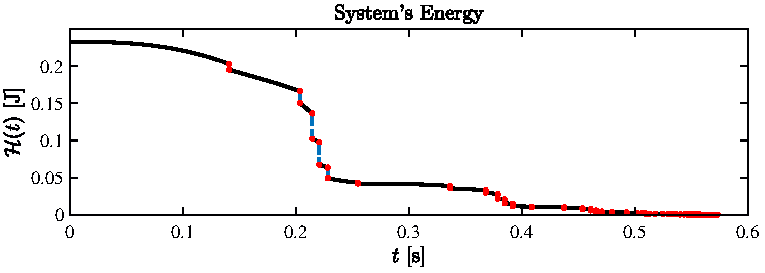
\includegraphics[width=\linewidth]{Figures/aut3.pdf}
	\caption[Uncontrolled system: time evolution of the Hamiltonian function]{Uncontrolled system: time evolution of the Hamiltonian function. Due to system's passivity, the energy monotonically decreases to zero both during flow and jumps.}
	\label{fig:aut3}
\end{figure}
%
\begin{figure}[hb!]
	\centering
	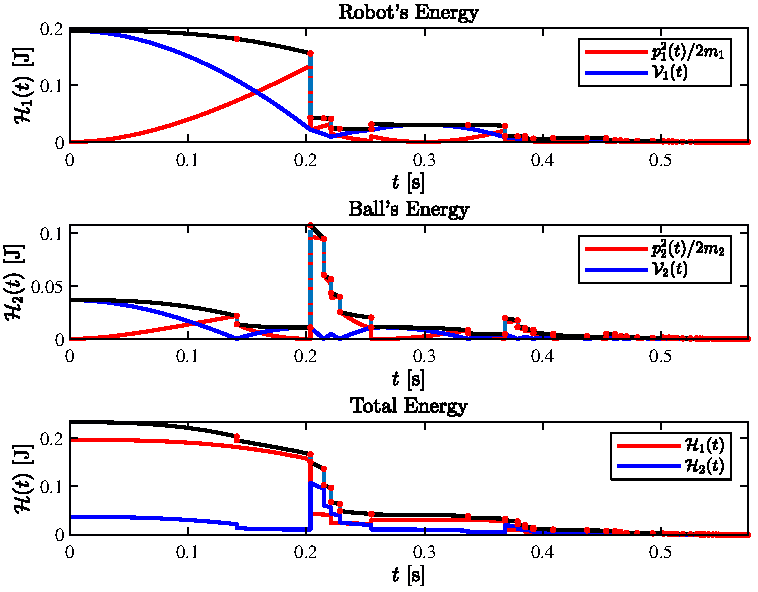
\includegraphics[width=\linewidth]{Figures/aut4.pdf}
	\caption[Uncontrolled system: Energy distribution within the system]{Uncontrolled system: Energy distribution within the system. Trajectories decrease on  level--sets of $\Ha$, even if $\Ha_1$ and $\Ha_2$ may locally increase after some ball--robot impacts.}
	\label{fig:aut4}
\end{figure}
Fig.~\ref{fig:aut3} pictures  the time evolution of the Hamiltonian function while Fig.~\ref{fig:aut4} shows how the energy is distributed within the system during its time evolution.
It can be noticed that $\Ha$ presents a monotonically decreasing trend, in both flows (due to the viscous friction terms) and jumps (since the restitution coefficients are less than one). In fact, trajectories decrease on level--sets of $\Ha$, even if $\Ha_1$ and $\Ha_2$ may locally increase after some ball--robot impacts. Moreover, from the figures it is easily to verify the asymptotic stability and attractivity of the origin ($x = \mathbb{0}_4$) and the \textit{Zeno behavior} of the autonomous system (see \cite{goebel2009hybrid}).


%%%%%%%%%%%%%%%%%%%%%%%%%%%%%%
\subsection{Controlled System}\label{sec:controlled_bd}
%
Simulations of the system controlled via iterative energy shaping have also been performed. The control parameters have been chosen as: $k_{p,w} = 10^4$, $k_{d,w} = 10^3$, $\delta = 0.05$m, $k_0 = 10$, $k_{d,h} = 0$, $\varphi_\xi(e) = 10e + 100\sum_{i = 1}^{\xi}e(i)$, $q_{2,max}^* = 0.1$m. The time evolution of the state variables are shown in Fig.~\ref{fig:ctrl1} and Fig.~\ref{fig:ctrl1_det}.
%
\begin{figure}[hb!]
	\centering
	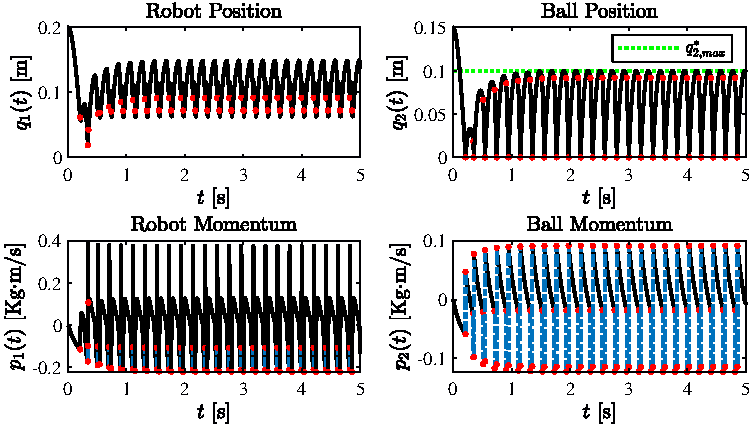
\includegraphics[width=\linewidth]{Figures/ctrl1.pdf}
	\caption[Iterative energy shaping control: time evolution of the robot and ball states]{Iterative energy shaping control: time evolution of the robot and ball states (position and momentum). Red dots correspond to system's jumps while dashed blue lines highlight discontinuous state changes. Notice that the ball states converge on a periodic trajectory reaching at each bounce the desired peak $q^*_{2,max}$ (dotted green line).}
	\label{fig:ctrl1}
\end{figure}
%
%
\begin{figure}[!ht]
	\centering
	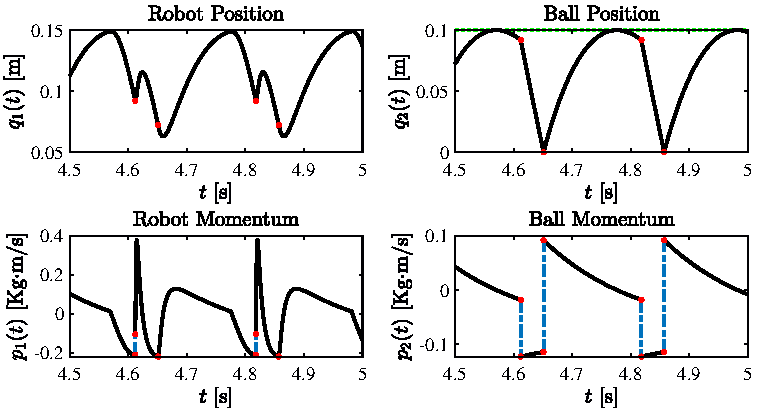
\includegraphics[width=\linewidth]{Figures/ctrl1_det.pdf}
	\caption[Iterative energy shaping control: detailed view of the time evolution of the ball and robot positions at steady state]{Iterative energy shaping control: detailed view of the time evolution of the ball and robot positions at steady state.}
	\label{fig:ctrl1_det}
\end{figure}
%
%
Notice that the trajectory of the ball becomes periodic (asymptotically), reaching at each bounce the desired peak $q_{2,max}^*$, proving the effectiveness of the proposed control scheme. Furthermore, the time evolution of the energy function is shown in Fig.~\ref{fig:ctrl3} and Figs.~\ref{fig:ctrl3_det} while Fig.~\ref{fig:ctrl4} and Figs.~\ref{fig:ctrl4_det} show how the energy flows across the system during each period. 
%
\begin{figure}[!b]
	\centering
	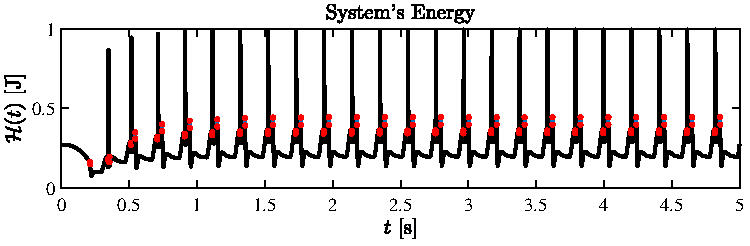
\includegraphics[width=\linewidth]{Figures/ctrl3.pdf}
	\caption[Iterative energy shaping control: the time evolution of the Hamiltonian function]{Iterative energy shaping control: the time evolution of the Hamiltonian function. After a short transient also the system's energy becomes periodic.}
	\label{fig:ctrl3}
\end{figure}
%
\begin{figure}[!ht]
	\centering
	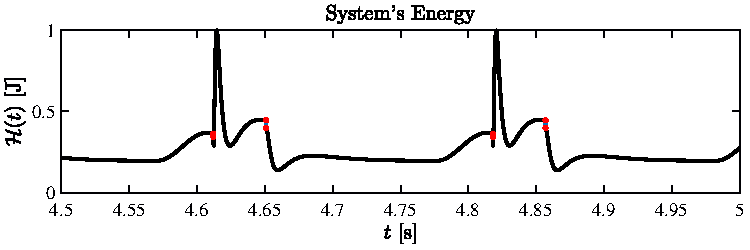
\includegraphics[width=\linewidth]{Figures/ctrl3_det.pdf}
	\caption[Iterative energy shaping control: detailed view of the the Hamiltonian at steady--state]{Iterative energy shaping control: detailed view of the time evolution of the Hamiltonian function at steady--state to highlight its (asymptotic) periodicity.}
	\label{fig:ctrl3_det}
\end{figure}
%
\begin{figure}[hb!]
	\centering
	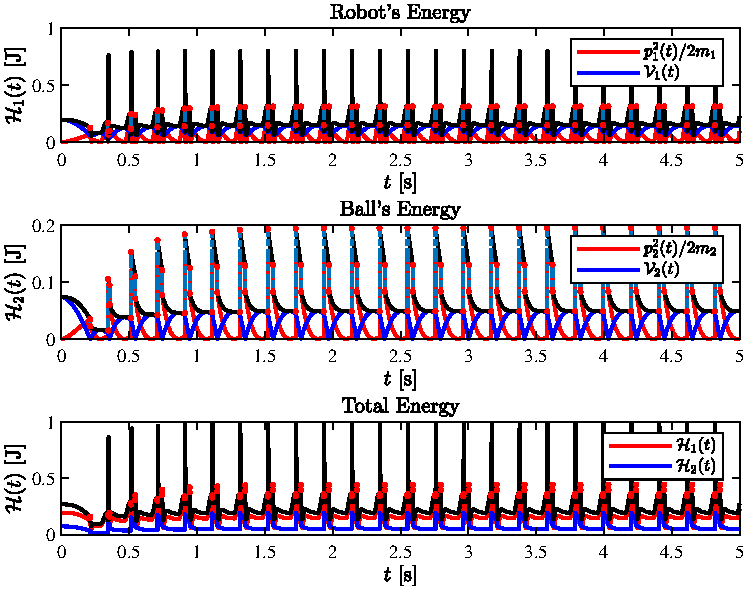
\includegraphics[width=\linewidth]{Figures/ctrl4.pdf}
	\caption[Iterative energy shaping control: Distribution of the energy across the system's components and time]{Iterative energy shaping control: Distribution of the energy across the system's components and time. After a short transient also the system's energy becomes periodic.}
	\label{fig:ctrl4}
\end{figure}
%
\begin{figure}[ht!]
	\centering
	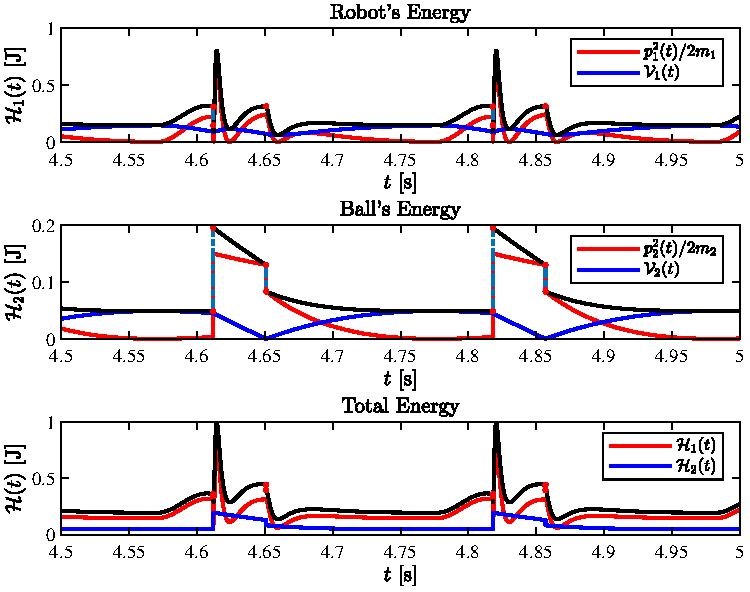
\includegraphics[width=\linewidth]{Figures/ctrl4_det.pdf}
	\caption[Iterative energy shaping control: detailed view of the energy distribution across the system's components and time]{Iterative energy shaping control: detailed view of the energy distribution across the system's components and time. at steady state to highlight its (asymptotic) periodicity.}
	\label{fig:ctrl4_det}
\end{figure}
As expected, also the energy becomes periodic. In fact, the energy at the beginning and at the end of each cycle (bounce) assumes exactly the same value. Moreover, it can be noticed that, at steady state, during the ball--robot impact, the robot transfers to the ball the exact amount of energy necessary to reach the desired bounce peak. Finally, as shown in Fig. \ref{fig:ctrl5} the error goes to zero with the number of cycles.
%
\begin{figure}[!ht]
	\centering
	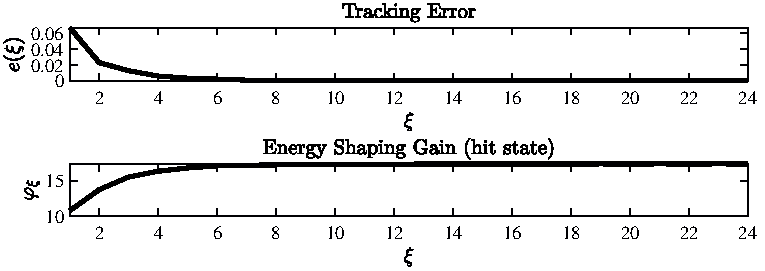
\includegraphics[width=\linewidth]{Figures/ctrl5.pdf}
	\caption[Iterative energy shaping control: (discrete) time evolution of the tracking error $e$ and of the energy shaping gain $\varphi_\xi(e)$]{Iterative energy shaping control: (discrete) time evolution of the tracking error $e$ and of the energy shaping gain $\varphi_\xi(e)$. As the number of cycles $\xi$ increases, the tracking error $e$, i.e. the difference between the desired and ball's bounce peak, goes asymptotically to zero. At the same time, the energy shaping gain converges, increasing monotonically, to a constant value.}
	\label{fig:ctrl5}
\end{figure}
%
On the other hand, the function $\varphi_\xi(e)$ converges exponentially to a positive constant value. 
%
\begin{figure}[ht!]
	\centering
	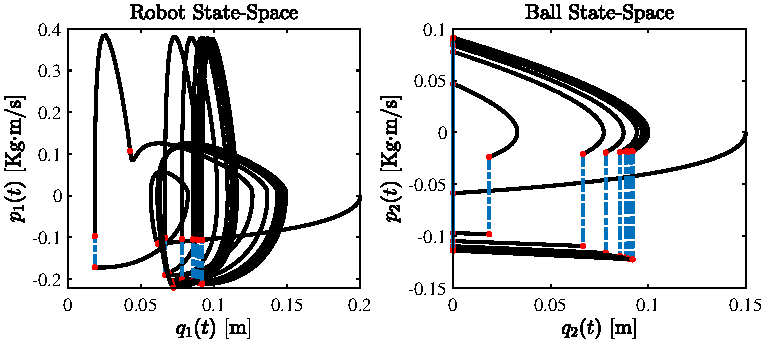
\includegraphics[width=\linewidth]{Figures/ctrl2.pdf}
	\caption[Iterative energy shaping control: phase--space trajectories]{Iterative energy shaping control: projections on the $q_1-p_1$ plane and the $q_2-p_2$ plane of the phase-space trajectory of the system. The system converges to a hybrid limit cycle in which $e=0$.}
	\label{fig:ctrl2}
\end{figure}
%
A final consideration about the convergence of the system to the desired periodic trajectory can be made from the phase-space portrait of the system's trajectory (Fig.~\ref{fig:ctrl2}). Being the time represented by the color transition, it can be noticed that the system approaches a limit cycle, an attractive asymptotically periodic trajectory, in which the tracking error is zero.



\subsection{Numerical Stability and Robustnes Analysis}
%
\subsubsection{Robustness to Initial Condition}
In order to numerically prove the stability and robustness of the proposed control scheme, a Monte Carlo experiment similar to the one presented in Section~\ref{sec:analysis_aut}, has been performed. In particular, choosing as physical parameters $m_1=0.1\text{Kg}$, $m_2=0.15\text{Kg}$, $\beta_1=0.2$, $\beta_2=0.3$, $c_1=c_2=0.8$ and control parameters $k_{p,w} = 10^4$, $k_{d,w} = 10^3$, $\delta = 0.5$, $\sigma = 10$, $k_{d,h} = 10^2$, $\varphi_\xi(e) = 3000 + 10e + 300\sum_{i = 1}^{\xi}e(i)$, $q_{2,max}^* = 1$, a total of 3000 trajectories have been computed starting from initial conditions $\xb_0^i$ sampled by the normal distribution
%
\begin{equation}
\N(\xb_0,\sigma\mathbb{I}_n),
\end{equation}
\begin{figure}[t!]
	\centering
	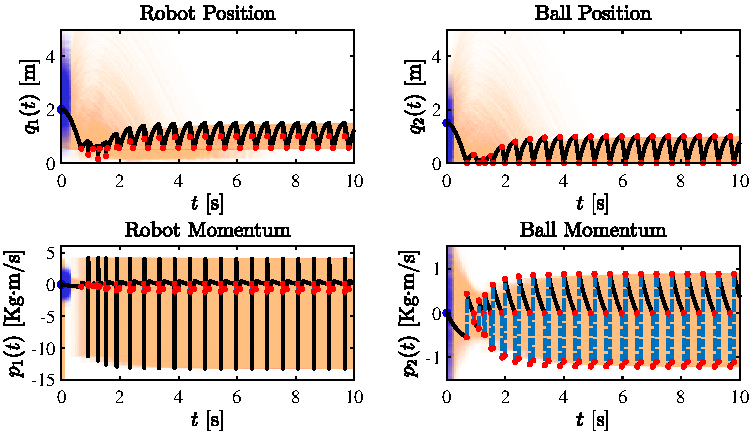
\includegraphics[width = \linewidth]{Figures/reg1.pdf}
	\caption[Time evolution of the controlled system' state in the Monte Carlo simulation]{Time evolution of the controlled system' state in the Monte Carlo simulation. The black trajectory is the nominal one (starting from $\xb_0$), where red dots and dashed blue lines indicate discrete events (impacts) and value of the state after the events, respectively. Orange lines show the traces of all the other trajectories of the Monte Carlo runs (with initial condition sampled from $\N(\xb_0,\sigma\mathbb{I}_n)$). The blue dots at $t=0$ are the initial conditions. It can be noticed how trajectories, starting far from each other, converge to the nominal trajectory.}
	\label{fig:reg1}
\end{figure}
with $\xb_0\triangleq(2,1.5,0,0)$ and $\sigma=1$\footnote{To minimize the effects of numerical instabilities of the \textit{HyEq} solver, larger physical and control parameters respect to the one used in the previous section have been chosen in this case.}. The time evolution of the system's state in the nominal case ($\xb(t=0) = \xb_0$) and all the Monte Carlo trials are displayed in Fig.~\ref{fig:reg1}.


It can be noticed how even if the trajectories start far from each other, are all asymptotically periodic and converge to the nominal trajectory. This means that the controller generates an attractive \textit{limit cycle} in the closed--loop system. This is further highlighted in Fig.~\ref{fig:reg2} where the phase--space trajectories are represented.

\begin{figure}[!ht]
	\centering
	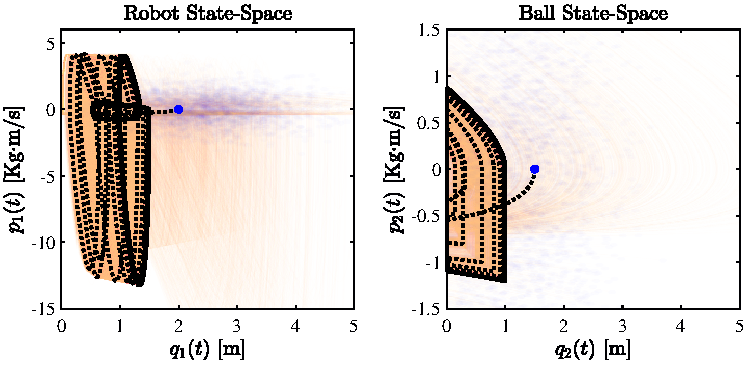
\includegraphics[width = \linewidth]{Figures/reg2.pdf}
	\caption[Phase--space trajectory of the controlled system in the Monte Carlo simulation]{Phase--space trajectory of the controlled system in the Monte Carlo simulation. The dashed black line is the nominal one (starting from $\xb_0$). Orange lines show the traces of all the other trajectories of the Monte Carlo runs (with initial condition sampled from $\N(\xb_0,\sigma\mathbb{I}_n)$). The blue dots at are the initial conditions. It can be noticed how trajectories, starting far from each other, converge to the nominal trajectory.}
	\label{fig:reg2}
\end{figure}

\begin{figure}[!hb]
	\centering
	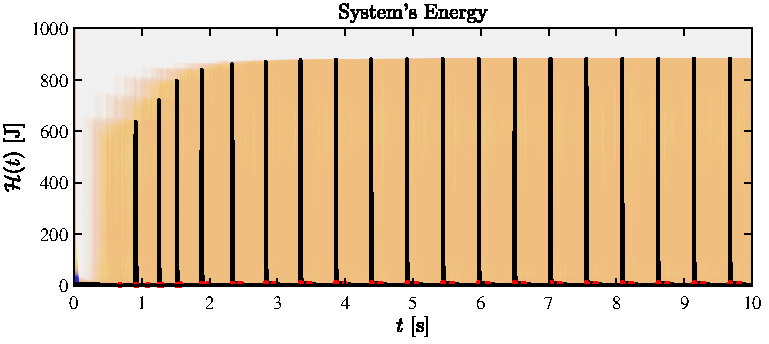
\includegraphics[width = \linewidth]{Figures/reg3.pdf}
	\caption[Time evolution of the energy in the Monte Carlo simulation]{Time evolution of the energy in the Monte Carlo simulation. The black trajectory is the nominal one (starting from $\xb_0$), where red dots indicate discrete events (impacts). Orange lines show the traces of all the other trajectories of the Monte Carlo runs (with initial condition sampled from $\N(\xb_0,\sigma\mathbb{I}_n)$). The blue dots at $t=0$ are the initial energies of each Monte Carlo run.}
	\label{fig:reg3}
\end{figure}

The time evolution of the energy (Hamiltonian function) among the Monte Carlo runs is also shown in Fig.~\ref{fig:reg3}.

The stability and attractivity to the nominal trajectory of the iterative energy shaping controlled system is shown in Fig.~\ref{fig:reg4}, which pictures the convergence of the tracking error and energy shaping gain. It is worth to underline that the mean of both, the error and gain among the Monte Carlo runs is almost identical to the nominal one. Further investigations might be interesting to be performed in order to analyse this phenomenon.
\begin{figure}[t!]
	\centering
	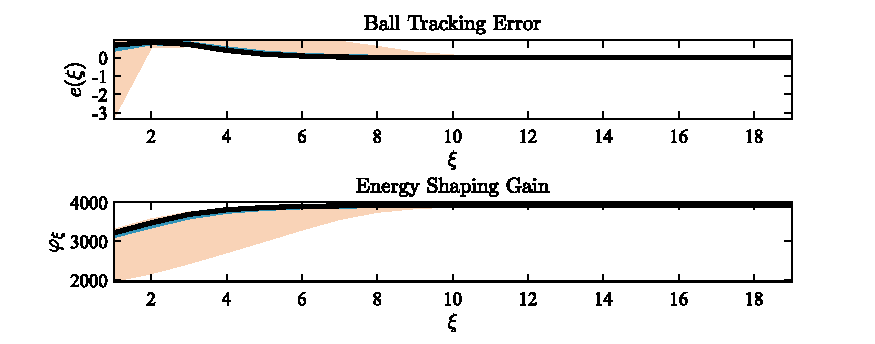
\includegraphics[width = \linewidth]{Figures/reg4.pdf}
	\caption[Convergence of the tracking error and controller gain in the Monte Carlo simulation]{Convergence of the tracking error and energy shaping gain (hit state) in the Monte Carlo simulation. The black line indicates the nominal case. The orange area bounds the minimum and maximum among the values of each Monte Carlo runs while the blue line represents their average.}
	\label{fig:reg4}
\end{figure}

\subsubsection{Robustness to Change of Parameters}
%
To prove the robustness against sudden changes of physical parameters of the system, several simulations have been performed with the same model and control parameters used in Subsection~\ref{sec:controlled_bd} and, changing at time $t = 2.5s$ some parameter of the model. Firstly the reference have been setted from $0.1$m to $0.05$m (-50\%). Then, the mass of the ball $m_2$ has been changed from $0.05$Kg to $0.25$Kg (+400\%). Finally, the restitution coefficient of the ball--robot collision has been changed from $0.8$ to $0.99$ (+23.75\%). The resulting states trajectories, tracking error, learned gains and energy are reported in Figs.~\ref{fig:roba},~\ref{fig:robb} and~\ref{fig:robc}.
% 
\begin{figure}[!ht]
	\centering
	\subfigure[States time evolution]{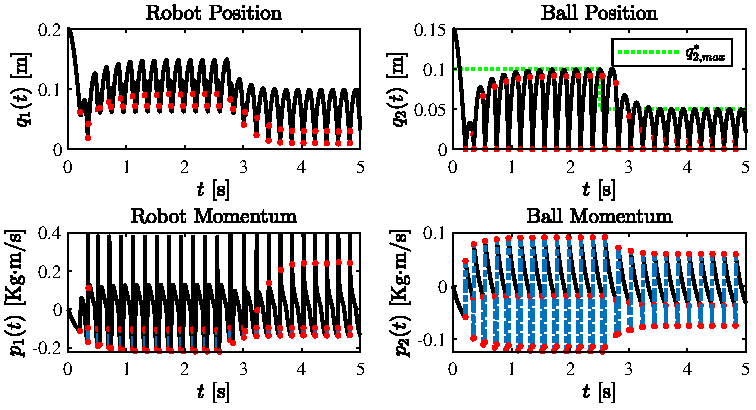
\includegraphics[width= .85\linewidth]{Figures/rob1.pdf}}
	\subfigure[Tracking error and learned gain]{\includegraphics[width= .85\linewidth]{Figures/rob2l.pdf}}
	\subfigure[System's energy]{\includegraphics[width= .85\linewidth]{Figures/rob3.pdf}}
	\caption[Robustness to parameters variations: reference position]{Robustness to parameters variations: change on the reference position.}
	\label{fig:roba}
\end{figure}
%
\begin{figure}[!ht]
	\centering
	\subfigure[States time evolution]{\includegraphics[width=.85\linewidth]{Figures/rob4.pdf}}
	\subfigure[Tracking error and learned gain]{\includegraphics[width=.85\linewidth]{Figures/rob5l.pdf}}
	\subfigure[System's energy]{\includegraphics[width=.85\linewidth]{Figures/rob6.pdf}}
	\caption[Robustness to parameters variations: ball's mass]{Robustness to parameters variations: change on the ball's mass.}
	\label{fig:robb}
\end{figure}
%
\begin{figure}[!ht]
	\centering
	\subfigure[States time evolution]{\includegraphics[width=.85\linewidth]{Figures/rob7.pdf}}
	\subfigure[Tracking error and learned gain]{\includegraphics[width=.85\linewidth]{Figures/rob8l.pdf}}
	\subfigure[System's energy]{\includegraphics[width=.85\linewidth]{Figures/rob9.pdf}}
	\caption[Robustness to parameters variations: restitution coefficients]{Robustness to parameters variations: change on the  restitution coefficients.}
	\label{fig:robc}
\end{figure}
%

Results demonstrated that the controller presents excellent robustness properties. In all three situations, the system recovers swiftly from the parameter change, adapting itself to the new value. 

In particular, when the reference is changed from $0.1$m to $0.05$m, all the physical properties of the system are conserved, e.g. dissipation during flows and jumps. However, to stabilize the ball on the desired trajectory, the robot needs to transfer less momentum to the ball during their collision. The system thus adapts itself to those new conditions by decreasing the energy shaping gain in the hit state. 

Instead, when the mass of the ball is increased from $0.05$Kg to $0.25$Kg, its momentum per unit of speed grows and thus, the conservation of momentum during the ball--robot collision requires an inresing of the robot's speed which will allow to transfer the same momentum to the ball. In turn, the acceleration of the robot during the hit mode is also controlled by the energy shaping gain. Consequently, it automatically increases and adpat itself towards the value of zero tracking error.

Finally, when the the ball--robot collision's restitution coefficient is increased from 0.8 to 0.99, the percentage of momentum that the robot transfers to the ball, i.e elasticity of impact, increases. Consequently, the energy shaping gain became lower.    
%
Robustness to changes in the robot mass, friction coefficients and ball--ground restitution coefficients have also been tested. Results shown the effectiveness of the proposed solution.
%
\clearpage
%%%%%%%%%%%%%%%%%%%%%%%%%%%%%%%%%%%%%%%%%%%%%%%%%%%%%%%%%%%%%%%%
\section{Summary}\label{sec:concl}
%
In this chapter, inspired by the theory developed in Chapter \ref{chap:HPH_systems}, a new paradigm of energy based control for the ball--dribbling robot, the \textit{iterative energy shaping}, has been introduced.
%
\newline

%
Firstly, the hybrid port--Hamiltonian model of the ball--dribbling robot has been derived and characterized. Then, its passivity and autonomous stability have been confirmed. It has been shown how chaotic behaviors arise in the autonomous model.

A new paradigm of energy--based control, the \textit{iterative energy shaping}, has been then introduced. Numerical simulations have been performed to prove the effectiveness of the proposed control scheme as well as its robustness to uncertain initial conditions and sodden changes to some physical parameters. 
\newline

%
The aim of the next chapter is to give an idea of the ubiquity of the hybrid port--Hamiltonian framework is. A novel hybrid nonlinear controller is developed to solve a theoretical problem for linear system. Then, it is shown that the controlled system belongs to the class of hybrid port--Hamiltonian systems. 